% This is an example of how to use the "npsthesis" document style for theses
% Modified for personal use by Fabrice Ardhuin, 2001/03/10
%
%  TO DO : add http://upload.wikimedia.org/wikipedia/commons/d/db/Munk_ICCE_1950_Fig1.svg  in ch1 

\documentclass[a4paper]{book}  % psfig for Encapsulated PostScript
%\usepackage{fullpage}
\addtolength{\oddsidemargin}{-0.4in} \addtolength{\evensidemargin}{-1.1in}
\addtolength{\textwidth}{1.5in} \addtolength{\topmargin}{-0.5in}
\addtolength{\textheight}{1.4in}
\usepackage[pdftex]{graphicx}
\usepackage{amsmath}
\usepackage{bm}
\pdfcompresslevel9
\usepackage[american]{babel}
% %\usepackage{upmath}
\usepackage[latin1]{inputenc}
%\usepackage[pdflatex]{graphics}
\usepackage{makeidx}
\usepackage{hyperref}
\usepackage{float}
\usepackage[section]{placeins}
 \usepackage{xcolor}
\hypersetup{
    colorlinks,
    linkcolor={red!50!black},
    citecolor={blue!50!black},
    urlcolor={blue!80!black}
}

%\usepackage[pdftex,plainpages=false]{hyperref}
\usepackage{natbib}
\setlength{\bibsep}{0em}

%\degree{Doctor of Philosophy In Oceanography}

% these macros save typing:
\newcommand{\beq}{\begin{equation}}
\newcommand{\beqa}{\begin{eqnarray}}
\newcommand{\eeq}{\end{equation}}
\newcommand{\eeqa}{\end{eqnarray}}
%
%\newcommand\p3{Part 3}
%\newcommand\p2{Part 2}
%\newcommand\p1{Part 1}

%   don't have right font for script R, so use:
\renewcommand{\Re}{{\cal R}}
\providecommand\boldsymbol[1]{\mbox{\boldmath $#1$}}
\providecommand\bnabla{\boldsymbol{\nabla}}
\providecommand\bcdot{\boldsymbol{\cdot}}
\providecommand\upi{\pi}
\newcommand\biS{\mathbf{S}}
\newcommand\cb{\mathbf{c}}
\newcommand\Cb{\mathbf{C}}
\newcommand\Mb{\mathbf{M}} 
\newcommand\dr{\mathrm{d}}
\newcommand\er{\mathrm{e}}
\newcommand\etb{\mathbf{\eta}}
\newcommand\ir{\mathrm{i}}
\newcommand\hu{\widehat{u}}
\newcommand\hv{\widehat{v}}
\newcommand\hw{\widehat{w}}
\newcommand\uL{\overline{u}^L}
\newcommand\wL{\overline{w}^L}
\newcommand\Eb{\mathbf{E}}
\newcommand\Sb{\mathbf{S}}
\newcommand\Ub{\mathbf{U}}
\newcommand\ub{\mathbf{u}}
\newcommand\xb{\mathbf{x}}
\newcommand\Kb{\mathbf{K}}
\newcommand\kb{\mathbf{k}}
\newcommand\kpb{\mathbf{k^{\prime}}}
\newcommand\lb{\mathbf{l}}
\newcommand\zerob{\mathbf{0}}
\newcommand\Deltab{\mathbf{\Delta}}
\newcommand\etal{\mbox{\textit{et al.}}}
\newcommand\etc{etc.\ }
\newcommand\eg{e.g.\ }
\newcommand\Real{\mathrm{Real}}
\newcommand\Frou{\mbox{\textit{Fr}}}  % Froude number
\newcommand\ttz{\ensuremath{\rightarrow 0}}
\newcommand\Ur{\mbox{\textit{Ur}}}  % Ursell number
\newcommand\Vb{\mathbf{V}}
\newcommand\zb{\overline{\zeta}}  
\newcommand\zL{\overline{\zeta}^L}

\def\sfbsL{\mathsfbi{L}}
\def\sfbsV{\mathsfbi{V}}
\def\sfbsD{\mathsfbi{D}}
\def\d{.}    % decimal mark

\newcommand{\boxedeqn}[1]{%
  \[\fbox{%
      \addtolength{\linewidth}{-2\fboxsep}%
      \addtolength{\linewidth}{-2\fboxrule}%
      \begin{minipage}{\linewidth}%
      \begin{equation}#1\end{equation}%
      \end{minipage}%
    }\]%
}


\begin{document}
\title{{\Huge Ocean waves in geosciences }
{\Large \\  parts 1 and 2: general wave topics from deep to shallow water}
 \vspace{3.0cm}\\
   \centerline{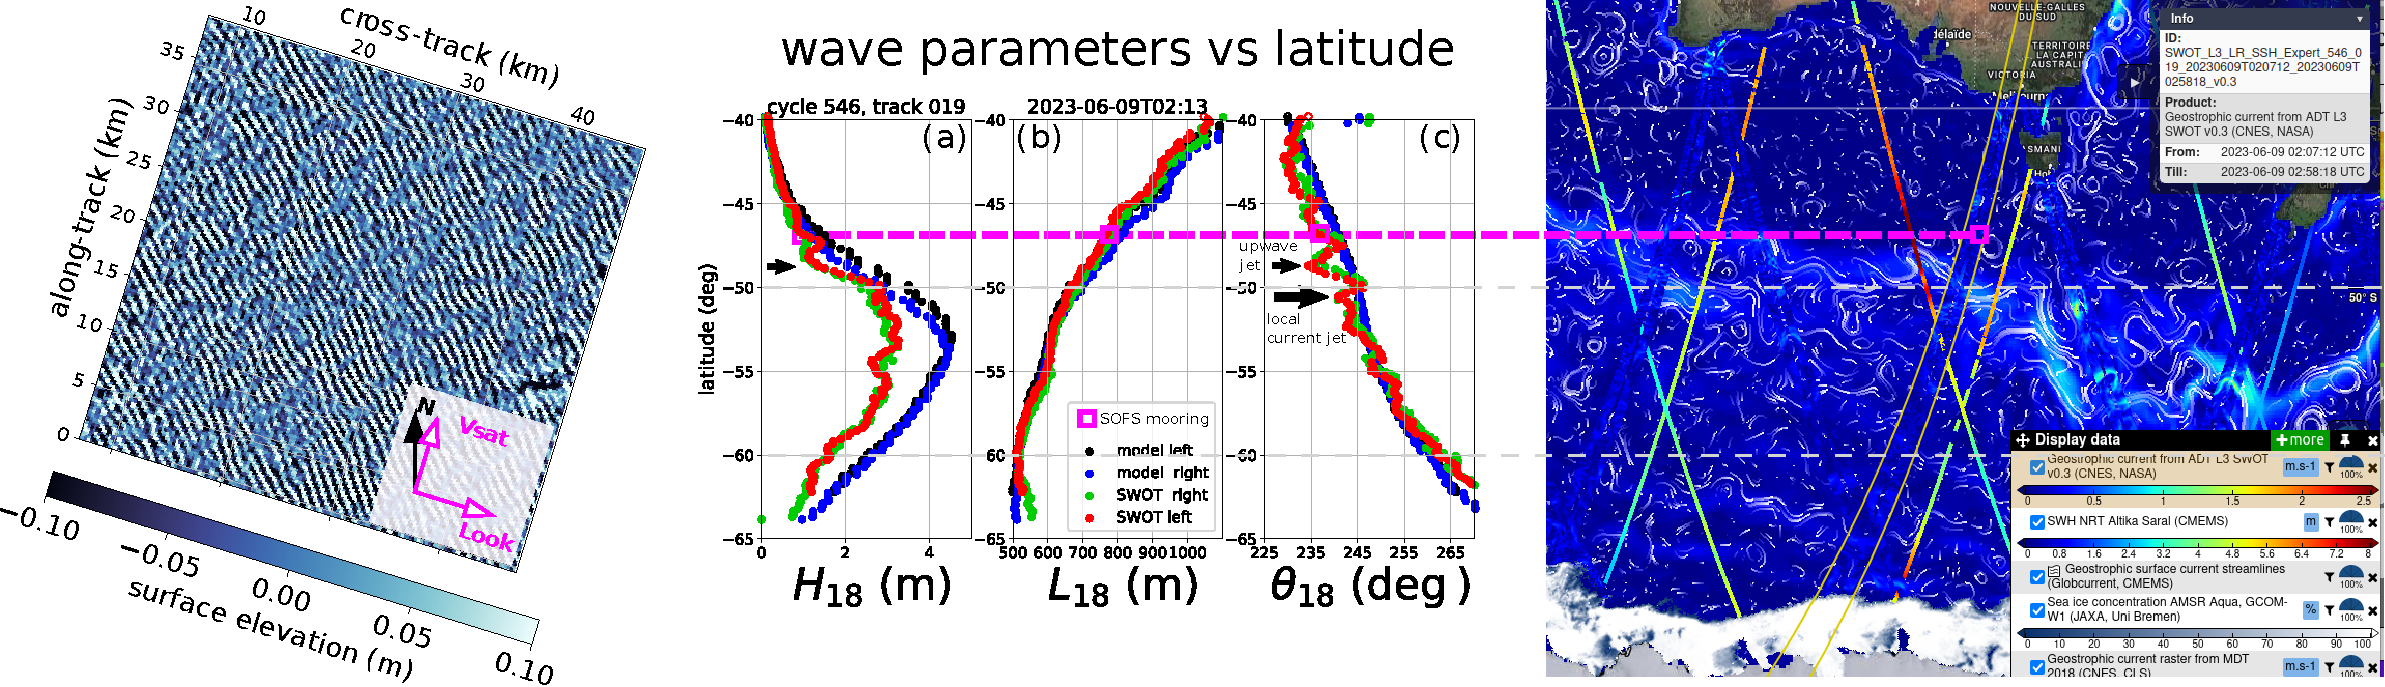
\includegraphics[width=\textwidth]{cover.pdf}}}
%%%%%%%%%%%%% figure
%\begin{figure}
%\centerline{\includegraphics[width=0.7\textwidth]{couv_cours.eps}}
%\vspace{3.64in}
%\end{figure}
%%%%%%%%%%%%% end of figure
\author{Fabrice Ardhuin, \\
\vspace{0.5cm}\\
Laboratoire d'Oc{\'e}anographie Physique et Spatiale, Brest,
France \\
\vspace{0.5cm}\\
doi:  10.13140/RG.2.2.16019.78888/11,  \url{https://github.com/ardhuin/waves_in_geosciences} \\
\vspace{1.5cm}\\
} \maketitle
\clearpage
On the cover: Left: swell waves from extratropical storm Rosemary resolved by the Surface Water Ocean Topography satellite, at the location of the Southern Ocean Flux Station mooring \citep{Hay&al.2023}, South of Australia, along track 19, on 9 June 2023. Center: from the resolved surface elevation map, one can estimate swell wave parameters, here for waves with periods longer than 18~s, and investigate their evolution along the satellite track. Such long waves waves are generated by the winds of the most powerful storm, and propagate across ocean basins where they are are also influenced by currents and sea ice. The right panel gives more context for these wave observations using the Ocean Virtual Laboratory developed by Oceandatalab: SWOT-derived currents confirm the presence of a current jet at 51$^\circ$ S, part of a southward meander of the Antarctic Circumpolar Current (ACC). Other satellite altimeters, here only SARAL is shown, also confirm the wave height reductions associated to refraction of the westerly waves in the ACC (\url{https://odl.bzh/WjEKPhZa}). More details on storm Rosemary and the capability of the SWOT satellite mission can be found in \cite{Ardhuin&al.2024}. 
 \cleardoublepage
\pagenumbering{roman}

\setcounter{page}{3}

\tableofcontents
\cleardoublepage


%\mainmatter
\setcounter{chapter}{0}

\pagenumbering{arabic}
\chapter*{Foreword}\label{foreword}
There are countless scholarly articles and books about ocean waves, with many different points of view, going from 
mathematical treatises to naval architecture. Among these we can single out the excellent textbooks by 
\cite{Kinsman1965}, \cite{Dean&Dalrymple1991},  
and \cite{Holthuijsen2007}, the engineering manual from the \cite{USACE2002}, and many excellent scientific 
monographs by \cite{Phillips1977}, \cite{Dingemans1997a}, \cite{Young1999}, \cite{Lavrenov2003}, \cite{Janssen2004}, \cite{Lannes2013} ...  

So why another one? 

First of all, scientific developments never stop, making these previous works not obsolete but less up to date 
and complete. This will happen with the present book, even if I am trying to update it on a regular basis. The parts 1 and 2 
and the associated teaching material (jupyter notebooks ...)  is designed to be at the level of Master students in oceanography. 

Second, and more important, all these books, except possibly the jewel by \cite{Phillips1977} have a rather narrow 
scope, and do not cover aspects for which no recent monograph exist. I particularly think about microseisms, infragravity waves or 
measurement techniques including satellite remote sensing. Some of these topics are only treated in part 3.

Working with coastal engineers, geomorphologists and seismologists, has motivated me to bring to 
the forefront those results that are often obscure or very hard to follow. My point of view is that 
ocean waves play a very particular role in the Earth System, both as an important element of air-sea or land-ocean exchanges, and also as a deforming mirror that 
modifies our measurements of ocean properties using remote sensing and even in situ techniques. As a result, much insight and cross-fertilization 
can come from the integration of many geoscientifc fields, from 
microseisms to remote sensing, as well as applied disciplines such as marine meteorology or coastal and ocean engineering.
At the very least, these different disciplines are providing new data, tools, and different points of view that complement each other 
in constraining  our physical understanding of wave processes, and the parameterizations used in numerical models or remote sensing algorithms. 

On these topics, I have tried to be clear without compromising the 
accuracy of the results, but this is a very difficult balance. If you find it unclear, do not hesitate to contact me
and I will try again to clarify in the next revision. I shall finish with a final warning:  my selection of topics is clearly biased to my own tastes and 
interests, which are clearly favouring geosciences versus engineering. It does not mean that the topics ignored here are not important. 
For example, a good discussion of 
extreme waves and sea state analysis would be much more useful for all engineers 
than our development on three-dimensional wave-current interactions. For this you may go to section 4.3 of \cite{Holthuijsen2007} or, with more details, to \cite{Boccotti2000}.
I hope that the present book will be a good combination 
of useful and interesting topics. \\

\vspace{0.5cm}
The document is organized in two parts, one relevant to waves in deep water, another providing additional 
information on coastal and shallow water aspects. Both are complemented by a separate book, which contains a third part that goes into some details that are probably not relevant for 
most readers, in particular Master students. 

The present book is designed to make it easier to read in electronic form, including hypertext links within the document 
and towards outside sources, such as the cited references. It is designed as a teaching material for the wave-related Master courses 
at University of Brest and ENSTA-Paris Tech. Because the present document is trying to follow the latest 
advances in research -- and my imperfect understanding of these. The permanent evolution unfortunately leads to the presence of errors, more so in part III. 
I thank 
Nicolas Rascle, Nadine Paugam, Cl�ment Gandon, Nobuhiro Suzuki, Sophia Brumer, Marine De Carlo and Oyvind Brevik for many corrections, Jean-Fran{\c c}ois Filipot for contributions and help in translating chapter 3, and 
Philippe Bonneton for discussions and help on the structure and contents of chapter \ref{ch_surf}.  
%This version is still not finished and some (old) parts in chapter 22-26 are still in French and will be translated in the coming months. OK, months may be years as I've been writing this for about ten years, but I'm not giving up hope.
I thank you in advance for finding any dubious or strange contents, or broken links.

\part{Waves in deep water} 
\cleardoublepage
\chapter{Introduction}\label{ch1}
\section{Waves in geosciences}
From the ripples on a water puddle to large breaking waves on the beach, we have all seen waves. 
They can be familiar or threatening, possibly deadly for seasoned fishermen or yachtsmen 
\citep[e. g. ][]{Pierson1972,Greenslade2001b}. Waves can exert huge forces: just try to stand up in the surf,
in front of a two-meter tall wave that breaks. And two meters is a far cry from the maximum recorded wave height at sea, towering
32~m above the following crest \citep{Liu&al.2008b}. The most severe \textit{sea state}, estimated from satellite radar altimetry, had a significant 
wave height of 18.5~m \citep{Hanafin&al.2012,DeCarlo&Ardhuin2024}, which, as we shall see in this chapter, 
means that some wave heights probably exceeded 35~m. Surfing contests have also focused on some specific coastal areas where waves are strongly amplified and produce waves of 30~m height or more, such as in Nazare, Portugal.



%%%%%%%%%%%%%%%%%%%%%%%%%%%%%%%%%%%%%%%%%%%%%%%%%%%%%%%%%%%%%%%%%%%%%%
\begin{figure}[htb]
\centerline{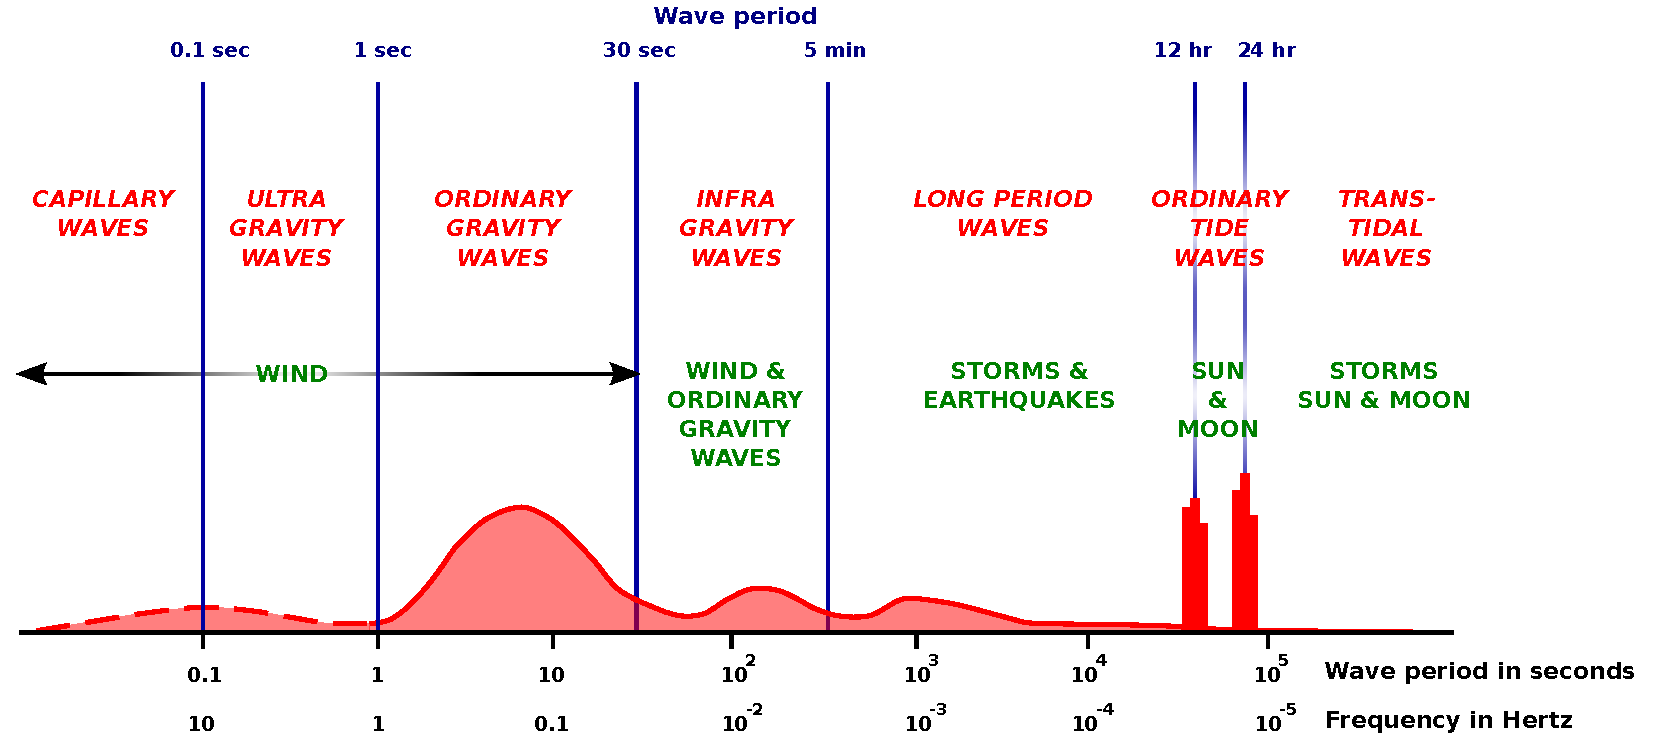
\includegraphics[width=\textwidth]{FIGS_CH_INTRO/Munk_ICCE_1950_Fig1.pdf}}
%\vspace{3.64in}
  \caption{Classification of ocean surface waves with usual names in red, as a function of wave periods (x-axis), with dominant forcing mechanisms in green. Adapted from \cite{Munk1950}.}
\label{fig:Munk1950}
\end{figure}
%%%%%%%%%%%%%%%%%%%%%%%%%%%%%%%%%%%%%%%%%%%%%%%%%%%%%%%%%%%%%%%%%%%%%%%%%
To be more precise, we need now to introduce some classification of the different wave motions. A simple classification, as proposed by 
\cite{Munk1950} and shown in figure \ref{fig:Munk1950}, is based on the typical time scales of between the passing of two crests. We shall call this time scale the wave period and denote it with the symbol $T$, even though the motion does not repeat itself exactly and is not mathematically speaking periodic. 

Figure \ref{fig:Munk1950} has boundaries between capillary waves, ultra gravity waves, ordinary gravity waves, infragravity waves and longer period waves (including tides) at periods of 0.1, 1, 30, and 300~s. Most of this book will focus on "ordinary gravity waves" with periods 1 to 30~s. As a physicist by training, I've never liked classifications with dimensional quantities that are often used in natural sciences: some of these distinctions are practically useful but they can be misleading.  Indeed, in some circumstances I would like to call "infragravity waves" some waves of periods around 10~s because they are generated by the same process as the "usual infragravity waves" with a period of 100~s. 

This period classification is closely related to a physical classification that distinguishes 
between the different  "restoring forces" which pulls back the surface towards a flat state, and the different generation processes for these waves. 
The two main restoring forces that we will consider are  \textbf{surface tension}, and \textbf{gravity}. Surface tension is mostly relevant for wave periods under 0.1~s, and will not be discussed much in the present book.

Once the restoring force is known, the next important things for any wave phenomenon are their
\begin{itemize}
          \item \textbf{generation},
          \item \textbf{propagation} 
          \item and \textbf{dissipation}.
         \end{itemize}
The goal of the present book is to describe and make understandable these 
three aspects, both qualitatively and quantitatively. 
This quantitative understanding allows an accurate forecast of local wave statistical properties, which we will 
call the sea state, as well as fluxes of energy and momentum between the atmosphere, ocean, sea ice, and solid Earth. 


In this book, we will restrict ourselves to waves which are more or less directly generated by the wind, leaving out 
tsunamis or ship wakes. But before leaving them out, let's say a few words about tsunamis. Tsunami propagation and dissipation properties 
are the same as the wind-waves described here, but whats sets them apart from wind-waves is their very large wavelength, 
which cannot be generated by wind in the same way as the usual wind-waves. Hence their generation mechanisms are specific, namely earthquakes, 
landslides, and meteorite 
impacts, which are all important but rare events, leading to very different statistical properties compared to the waves continuously 
generated by the wind. Another slightly more common source of meteo-tsunamis are abrupt changes in wind properties. 
All these generation events are transient, and typically cause a depression or bump of the sea surface that appears very fast but on a very 
large scale. This depression or bump then radiates a train of waves, with a period of the order of 10 minutes that is given by the size 
of the initial surface perturbation. These waves are strongly amplified in shallow water. The first perturbation to arrive on land can be a trough. 
If you see the sea retreating rapidly, this is it ... do not rush out to pick up crabs, but instead run to high ground, as a big crest will 
likely follow and flood what was the dry land. 

Instead of these transient wave trains, wind-generated waves are incessant and irregular.
The  time between the passing of two crests, which we define as the period $T$,  is typically less than 30~s. This limit is related 
to wind speeds, as explained in chapter \ref{ch_sourceterms}. 
These wind-waves also give rise to infra-gravity waves of periods 10~s to 10~minutes. For all these motions 
the average distance between two crests, which we shall call the mean wavelength $L_m$, increases with the mean period $T_m$. 
This wavelength goes from a few millimeters to about 1.2~km \citep{Ardhuin&al.2024}. For wave shorter than a few centimeters, the effect of surface 
tension must be taken into account, and these short waves are called gravity-capillary waves, and capillary waves when gravity can be neglected. 

Indeed, the \textbf{propagation} properties of waves is related to the balance of forces near the air-sea interface. If gravity or surface tension is the dominant force then the propagation is different.
Gravity fights against surface slopes, setting up a pressure gradient that tends to reduce the sea level slope and is the main force 
for large wavelengths. Surface tension, instead, fights against surface curvature:
it arises from the difference in thermodynamic properties of the interface between the two fluids, that are air and water. 
This difference gives an energy to their interface, which is proportional to the area of the interface: the more curved the surface the 
larger the surface energy. This surface energy is, for capillary waves, the equivalent of the gravitational potential energy. This force explains 
why water droplets are spherical: the sphere is the shape that minimizes the area (hence the energy) for a given volume. 
This surface tension also explains why short breaking waves are not energetic enough to generate bubbles and foam at the sea surface. 
The presence of a continuous layer of ice can also act like an elastic layer with an effect similar to surface tension. In this case
even long waves can be influenced by the elasticity of the ice layer, this influence depends on the ice thickness \citep[e.g.][]{Squire&al.1995}. 
Because curvature is the second derivative of the surface elevation, surface tension effects are much stronger than gravity for small scales. 

Whether gravity or surface tension is the main restoring force, the work of these forces produces a motion with an associated kinetic energy. 
The oscillations of the air-sea interface are thus maintained by an exchange between potential and kinetic energy, 
until this energy is \textbf{dissipated}. Our waves are thus surface gravity waves, gravity-capillary or capillary waves for the shortest. 

In the family of gravity waves, at the other extreme towards the large scales, the slow oscillations on time scales of several hours to several days 
are also influenced by 
the Coriolis force, caused by the rotation of the Earth, and the waves become inertial-gravity waves, also known as Kelvin and Poincar{\'e}
waves. The main \textbf{generation} forces for these are the wind and the difference in the gravitational pull exerted by the Moon and Sun on the 
center and the surface of the Earth. Kelvin waves share many properties of gravity waves.

%%%%%%%%%%%%%%%%%%%%%%%%%%%%%%%%%%%%%%%%%%%%%%%%%%%%%%%%%%%%%%%%%%%%%%
\begin{figure}
\centerline{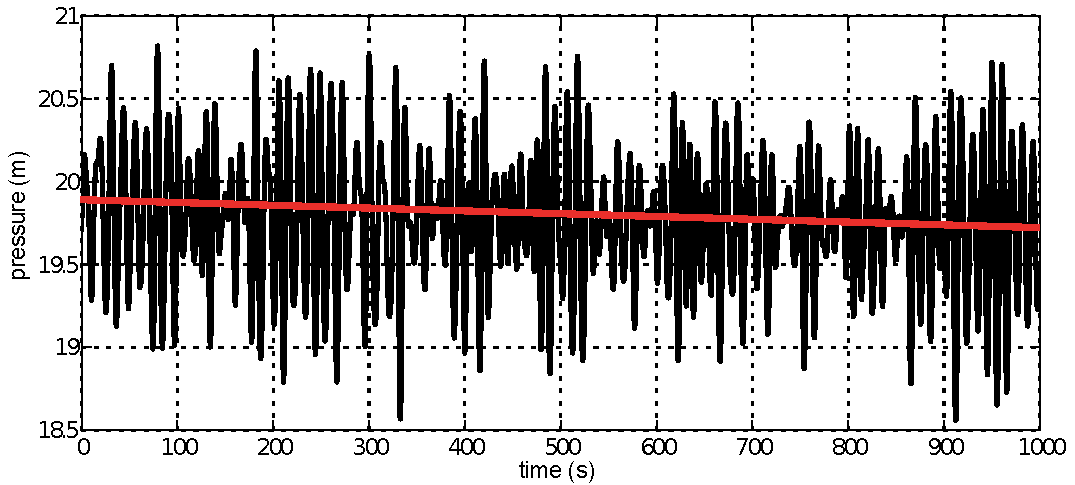
\includegraphics[width=\textwidth]{FIGS_CH_INTRO/p_at_berth1_en.pdf}}
%\vspace{3.64in}
  \caption{Example of the evolution of the bottom pressure in about 20~m of water 
 in Bertheaume bay, France, on January 31, 2004.}{The pressure in Pascals was converted here to an equivalent water height in meters
by dividing the absolute pressure 
recorded by a Nortek Vector %Seabird 26 
instrument, by the product $\rho_w g$ of water density $\rho_w \simeq 1026$kg/m$^3$, 
and gravity $g\simeq 9.81$m/s$^2$, after subtracting the atmospheric pressure recorded nearby, $p_a \simeq 10^5$Pa.  The 
fast oscillation caused by a swell of significant wave height $H_s=2.85$~m is superimposed on the tide 
that is gently falling, about 20~cm in 20~minutes, as shown by the red line.}
\label{pexemple}
\end{figure}
%%%%%%%%%%%%%%%%%%%%%%%%%%%%%%%%%%%%%%%%%%%%%%%%%%%%%%%%%%%%%%%%%%%%%%%%%

In practice, all these waves co-exist. Fortunately, it is often easy to sort them out and study them separately. 
Wind-waves and tides have very different periods and wavelengths, as illustrated by figure 
\ref{pexemple}. There is no such clear separation between capillary and gravity waves, except at low wind speeds 
when there is clear gap in the wave spectrum around the wavelength of 1.7~cm. For waves longer than 20~cm, 
we will ignore the effect of the surface tension which will greatly simplify our calculations. 
However, surface tension should not be ignored in general, in particular when considering 
wave dissipation by breaking and the effects of small scale surface roughness, both important for air-sea fluxes and remote sensing 
of the ocean surface.

The \textbf{propagation} of waves are generally well known thanks to the works of Laplace, Poisson, Stokes, Airy, Rayleigh and Boussinesq in 
the 18th and 19th centuries, with many later refinements. For a historical perspective, you may read the works of  \cite{Darrigol2003} and \cite{Craik2004}, and specific problems and questions are still open. The questions of  \textbf{generation} and \textbf{dissipation} are very active
research topics, with a fundamental problem posed by the multi-scale nature of real ocean waves: how short waves influence long waves and vice versa is 
very difficult to measure and analyze. Because of the strong demand for results, successful forecasting methods have been developed on more or less empirical grounds. 
Modern wave forecasting started with swell forecasts
for Morocco, in the 1920s \citep{Gain1918,Montagne1922}. This approach was generalized by 
\cite{Sverdrup&Munk1947} who considered the full life cycle of waves, from generation by the wind to dissipation 
in the middle of the ocean and on beaches. This latter work was 
motivated by the planning of the allied amphibious operation Torch in Morocco in 1942, which led to a method later applied to Normandy 
and many Pacific islands \citep{Bates1949}. Their British colleagues, forming the W group at the Admiralty, included Deacon, Darbyshire, Barber, Ursell and Longuet-Higgins  
who developed similar methods and introduced the spectral analysis of waves in 1945 \citep{Ursell1999}, paving the way for 
today's numerical wave models. The first numerical spectral wave model was developed by \cite{Gelci&al.1957}, the group that continued the Morocco wave forecasting effort in Casablanca.


Knowing and predicting the properties of waves is necessary for sea-going operations, the design of any marine structure such as 
a jetty, an offshore platform or a ship. Because waves are generated by the wind, there is an only tradition of telling the wind speed from the geometry of the waves, this is widely known as the Beaufort scale, reproduced in Table \ref{table_Beaufort} from \cite{Alcock&Morgan1978}. 

%%%%%%%%%%%%%%%%%%%%%%%%%%%%%%%%%%%%%%%%%%%%%%%%%%%%%%%%%%%%%%%%%%%%%%%%%%%%
\begin{table}
  \centering
  \begin{tabular}{|c|c|c|l|}
\hline
 Beaufort & descriptive     & wind speed  & specification for observation (open sea)  \\
 number   & term            &  (m/s)      &   \\
\hline
0               & Calm             &  0-1               & Sea like a mirror          \\
1               & Light air        &  1.5-2.5           & Ripples with the appearance of scales are formed \\
                &                  &                    & but without foam crests \\
2		& Light breeze     & 3 --4 		& Small wavelets still short but more pronounced; \\
                &                  &                    & crests have a glassy appearance and do not break \\
3               & Gentle breeze    & 4.5 --6            &  Large wavelets; crests begin to break;  foam of  \\
                &                  &                    & glassy appearance, perhaps scattered white horses \\
4		& Moderate breeze  & 6.5--8             &  Small waves becoming longer, fairly frequent white horses \\
5               & Fresh breeze     & 8.5-10.5           & Moderate waves, taking a more pronounced long form; \\
                &                  &                    & many white horses are formed (chance of some spray) \\
6               & Strong breeze    & 11--13.5           & Large waves begin to form; the white foam crests \\
                &                  &                    & are more extensive everywhere  (probably some spray)\\
7               &    Near gale     & 24--16.5           & Sea heaps up and white foam from breaking waves begins \\
                &                  &                    & to be blown in streaks along the direction of the wind \\
8               & Gale             & 17--20             & Moderately high waves of greater length; edges of crests \\
                &                 &                     & begin to break into the spindrift; the foam is blown in  \\
                &                &                    &  well-marked streaks along the direction of the wind  \\
9               & Strong gale     & 20.5--23.5         & High waves; dense streaks of foam along the direction of \\
                &                 &                    & the wind; crests of waves begin to topple, \\
                &                 &                    &tumble and roll over'; spray may affect visibility  \\
10              & Storm            & 24-27.5            & Very high waves with long overhanging crests; \\
                &                   &                  & the resulting foam, in great patches, is blown in dense \\
                &                  &                 & white streaks along the direction of the wind; on the whole \\
                &                  &                  & the surface of the sea takes on a white appearance; \\
                &                  &                  & the tumbling of the sea becomes heavy and shock-like; \\
                &                  &                  & visibility affected\\
11              & Violent storm    & 28--31.5           & Exceptionally high waves (small and medium-sized ships\\
                &                  &                    & might be for a time lost to view behind the waves); \\
                &                  &                    & the sea is completely covered with long white patches of \\
                &                  &                    & foam lying along the  direction of the wind; everywhere \\
                &                  &                    & the edges of the wave crests are blown into froth; \\
                &                  &                    &  visibility affected \\
12              & Hurricane        & 32 and over        &  The air is filled with foam and spray; sea completely \\
                &                  &                   &  white with driving spray; visibility very seriously affected  \\ 
\hline
\end{tabular}
\caption{The Beaufort scale for wind speed reproduced from \cite{Alcock&Morgan1978}. \label{table_Beaufort}}
\end{table}
%%%%%%%%%%%%%%%%%%%%%%%%%%%%%%%%%%%%%%%%%%%%%%%%%%%%%%%%%%%%%%%%%%%%%%%%%%%%

 Using the geometry of the waves and/or the properties of foam on the surface is still very much how we measure winds from satellite data, using scatterometers that measure the power of the radar echoes from the sea surface, or radiometers that measure the brightness temperature of the ocean surface. The relation between wind speed and those measurements
  is not unique because the waves may be at different stages of development. There is also a Beaufort scale for wave heights given in table \ref{table_seastate}, and clearly there is no one to one relationship between winds and waves. 


%%%%%%%%%%%%%%%%%%%%%%%%%%%%%%%%%%%%%%%%%%%%%%%%%%%%%%%%%%%%%%%%%%%%%%%%%%%%
\begin{table}
  \centering
  \begin{tabular}{|c|c|c|c|}
\hline
    \multicolumn{3}{|c|}{Wind sea} \\
 \hline
S code & descriptive term & wind sea wave height in meters (well developed)  \\
0 & calm (glassy)         & 0 \\
1 & calm (rippled)        & 0--0.1\\
2 & smooth (wavelets)     & 0.1--0.5 \\
3 & Slight                & 0.5--1.25  \\
4 & Moderate              & 1.25 --2.5  \\
5 & Rough                 & 2.5--4 \\
6 & Very Rough            & 4--6  \\
7 & High                  & 6--9 \\
8 & Very high             & 9--14  \\
9 & Phenomenal            & Over 14  \\
\hline
\end{tabular}
\caption{The Beaufort scale for sea states: source World Meteorological Organization, table 3700 \label{table_beaufort}}
\label{table_seastate}
\end{table}
%%%%%%%%%%%%%%%%%%%%%%%%%%%%%%%%%%%%%%%%%%%%%%%%%%%%%%%%%%%%%%%%%%%%%%%%%%%%


Waves modify the fluxes of momentum between the ocean and atmosphere and thus influence more or less directly the oceanic and 
atmospheric circulation. Waves are also an important agent in the pick-up and transport of sediments, and 
the main source of background seismic motions. 


Today, we can forecast with good confidence the main properties of the sea state and its consequences, including forces on a structure 
at sea, ship motions, working range of a radar... although the details of the generation and dissipation processes are not well known. 
This is a tribute to the flair of those who invented rules and equations to represent the complex and poorly known reality. 
However, given this empirical part, it is not surprising that the same models may not be accurate for secondary properties of the sea state, such as the distribution 
of the energy radiated in different directions or the statistics of short breaking waves. 


Going against the long-term specialization and separation of geosciencies in many sub-disciplines, 
there has been a strong interest since the late 1990s in the interaction of waves with the atmosphere, ocean currents, 
turbulence, sediment motion, from the scale of the global ocean to the small scale of any particular beach. This is motivated by 
integrated approaches for climate projections or the understanding of sediment transport from sources to sinks. 
These efforts should be continued to properly understand the interactions of waves and turbulence, and the multi-scale 
properties of the ocean surface. 
We hope that after reading the present book, that gives a broad view of what is known and tries to highlight what is still unclear,
the reader will gather the courage to continue the exploration of ocean waves after Stokes, Boussinesq, Munk, Longuet-Higgins,
Hasselmann, Zakharov, Katsaros, Phillips and many other less famous scientists who made today's knowledge possible. 

Courage, though, may not be enough, and some tools will be needed to start for this journey, including 
a working knowledge of calculus and fluid mechanics. 

The following books should be consulted for complements on different topics, 
\begin{itemize}
\item \cite{Kinsman1965} on general principles and wave measurements, in particular with arrays of sensors. Although a bit 
old, this book is very well written and easy to get into. 
\item \cite{Phillips1977} for a comprehensive view, although not up to date, of upper ocean processes (waves, internal waves, turbulence ...) 
\item \cite{Mei1989} for wave propagation, mass transport and wave-structure interactions
\item \cite{Dean&Dalrymple1991} gave a real textbook oriented towards engineering applications
\item \cite{WAMBook} gives the fundamental -- but not basic -- concepts of numerical wave prediction 
in the open ocean, this is not an easy read
\item \cite{Komar1998} wrote a nice textbook for coastal geomorphology, an excellent starting point for those 
who do not have a strong physics background
\item \cite{Young1999}  combined deep and shallow water waves, including also global wave climatology. 
\item the Coastal Engineering Manual \citep{USACE2002}, replaced the Shore Protection Manual. This book 
is edited by the U.S. Army Corps of Engineers, the body in charge of shoreline defenses and management of 
ports and waterways. This combines general principles with empirical formulas for coastal engineering. This is 
freely available on the web. 
\item \cite{Janssen2004} gives his perspective on wind and wave forecasting, with many theoretical details on wind-wave 
generation and nonlinear wave evolution. 
\item \cite{Holthuijsen2007} A very well illustrated textbook centered on numerical wave modelling, specifically for coastal 
environments, although a bit weak on physical processes, such as bottom friction.  
\end{itemize}
A lot of interesting material and teaching aids can be found on the web, from Tony Dalrymple's Java applets, to the UCAR Meted program 
targeted at meteorologists. A list of useful links will be proposed separately for each chapter. 

Let us now beg the tides and currents to stop their flow, so that we may study waves quietly. We will see later, in chapters \ref{ch_current} and 
\ref{ch_littoral} how waves interact with other oceanic motions. 

\section{Wave motion: some observations}
The random nature of ocean waves has long puzzled observers and made difficult all scientific investigations. 
Figure \ref{pexemple} gives a good example of a random sequence of high and low waves. Initially  
the forecasting of waves was formulated in terms of the highest wave. The notion of wave height distribution was only introduced after 1945, 
thanks to the development of wave recording devices, and the availability of computing power. Two types of methods have been developed to 
represent the random nature of the wave field. 
One of these is the spectral analysis, which will be heavily used in the following chapters. The other, is the wave-by-wave analysis, 
which we briefly describe here. More recent time-frequency analyses are a kind of hybrid of these two methods. 


Both methods are very useful and have their own limitations. Spectral analyses are well suited for the wave forecasting, in 
particular at large scales, because it explicitly represents the dispersion of waves that have different periods. 
Spectral analysis decomposes the sea surface in elementary sinusoidal waves, it is thus very important to know the properties of these 
sinusoidal waves. This is the topic of chapter \ref{ch1b}.
However, some sort of wave-by-wave analysis must be use to investigate localized 
events associated to the finite amplitude of the waves, such as breaking, as discussed in chapter \ref{ch_sourceterms}. 

%%%%%%%%%%%%%%%%%%%%%%%%%%%%%%%%%%%%%%%%%%%%%%%%%%%%%%%%%%%%%%%%%%%%%%%%%%%%%
\begin{figure} \label{FigWaveriderTSz}
\centerline{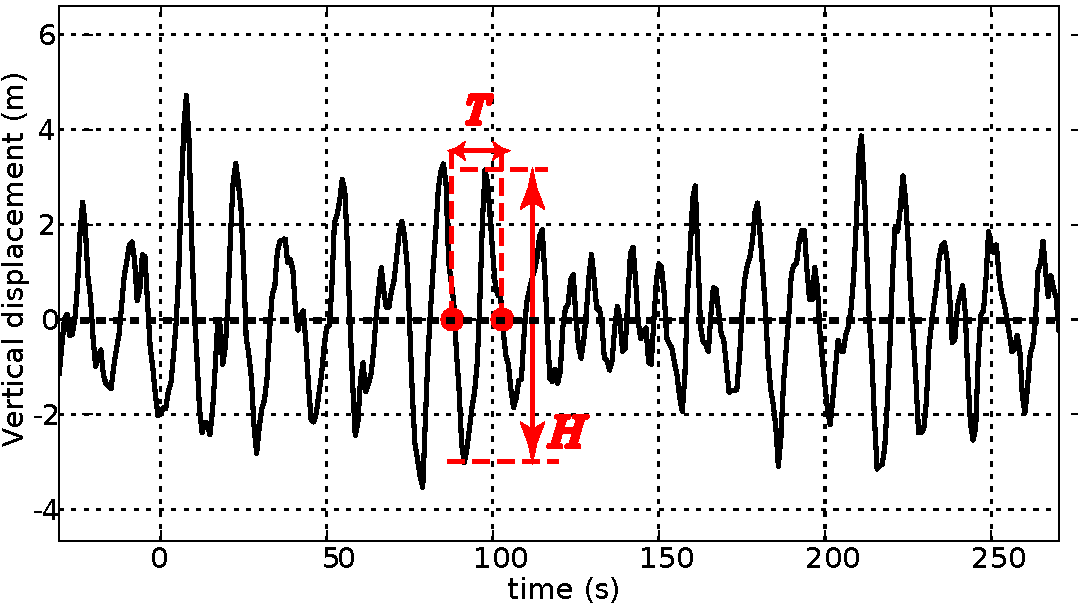
\includegraphics[width=0.8\textwidth]{FIGS_CH_INTRO/Exemple_DWIROISE2004_en.pdf}}
%\vspace{3.64in}
  \caption{Principle of wave by wave analysis: a series of elevation records is broken in individual waves of duration $T$. The separation from one 
wave to the next is the zero down-crossing of the vertical displacement. This example was obtained from a Datawell Waverider buoy deployed offshore 
of Crozon, France, in May 2004.}\label{fig:zero_crossing}
\end{figure}
%%%%%%%%%%%%%%%%%%%%%%%%%%%%%%%%%%%%%%%%%%%%%%%%%%%%%%%%%%%%%%%%%%%%%%%%%%%%%


\section{Wave-by-wave analysis\label{anavague}}
\subsection{Time series}
Time series are the most common type of measurement these days, let us see what we can learn about waves from time series. 
We shall work with series of sea surface elevation, but we could have used any other physical quantity such as the 
velocity or pressure in the water or in the air. 

We first define a single wave in time series by the time interval between two consecutive 
crossings of the mean sea level as the surface goes down, as illustrated in Fig. \ref{fig:zero_crossing}. 
The choice of 'down' instead of 'up' is fairly arbitrary but it 
keeps the forward face of the wave, which is usually  more interesting, within a single wave, whereas the rear face is split 
between two consecutive waves. 
For each wave we define a period $T$, which is the length of the time interval, and a height $H$, which is the 
difference between the maximum elevation (the crest) and the minimum elevation (the trough) during the perid. 



From a sequence of heights, we can define a probability density function (PDF) $dP$ as the limit, when $dH$ 
goes to zero, of the probability $P$ that a wave height is between $H$ and $H+dH$, divided by $dH$. 
For a statistically stationary sea state, the surface elevation is well approximated by the sum of  a large number 
of sine waves which are independent from one another. Applying the central limit theorem to this 
approximate model, we find that the surface elevation is a Gaussian process, with negative and positive anomalies around the mean sea level 
with statistics defined uniquely by the standard deviation of the sea surface elevation. As a result, and this was proven in the narrow frequency band limit 
by \cite{Rice1944} and \cite{Cartwright&Longuet-Higgins1956}, the heights follow a Rayleigh distribution, as shown on figure \ref{fig:Rayleigh}, 
 \begin{equation}
dP(H)=\frac{2H}{H_{\mathrm{rms}}^2}
\exp^{-{H^2}/{H_{\mathrm{rms}}^2}}.
\end{equation}
This PDF is normalized to give 
$\int_0^\infty dP dH =1$. The Rayleigh distribution is generally a good approximation for 98\% of the distribution, sometimes even more. 
For extreme values, a better approximation was given by \cite{Tayfun1980}, taking into account the correlations among wave components due to 
second-order nonlinearities. 
%%%%%%%%%%%%%%%%%%%%%%%%%%%%%%%%%%%%%%%%%%%%%%%%%%%%%%%%%%%%%%%%%%%%%%%%%%%%%
\begin{figure}
\centerline{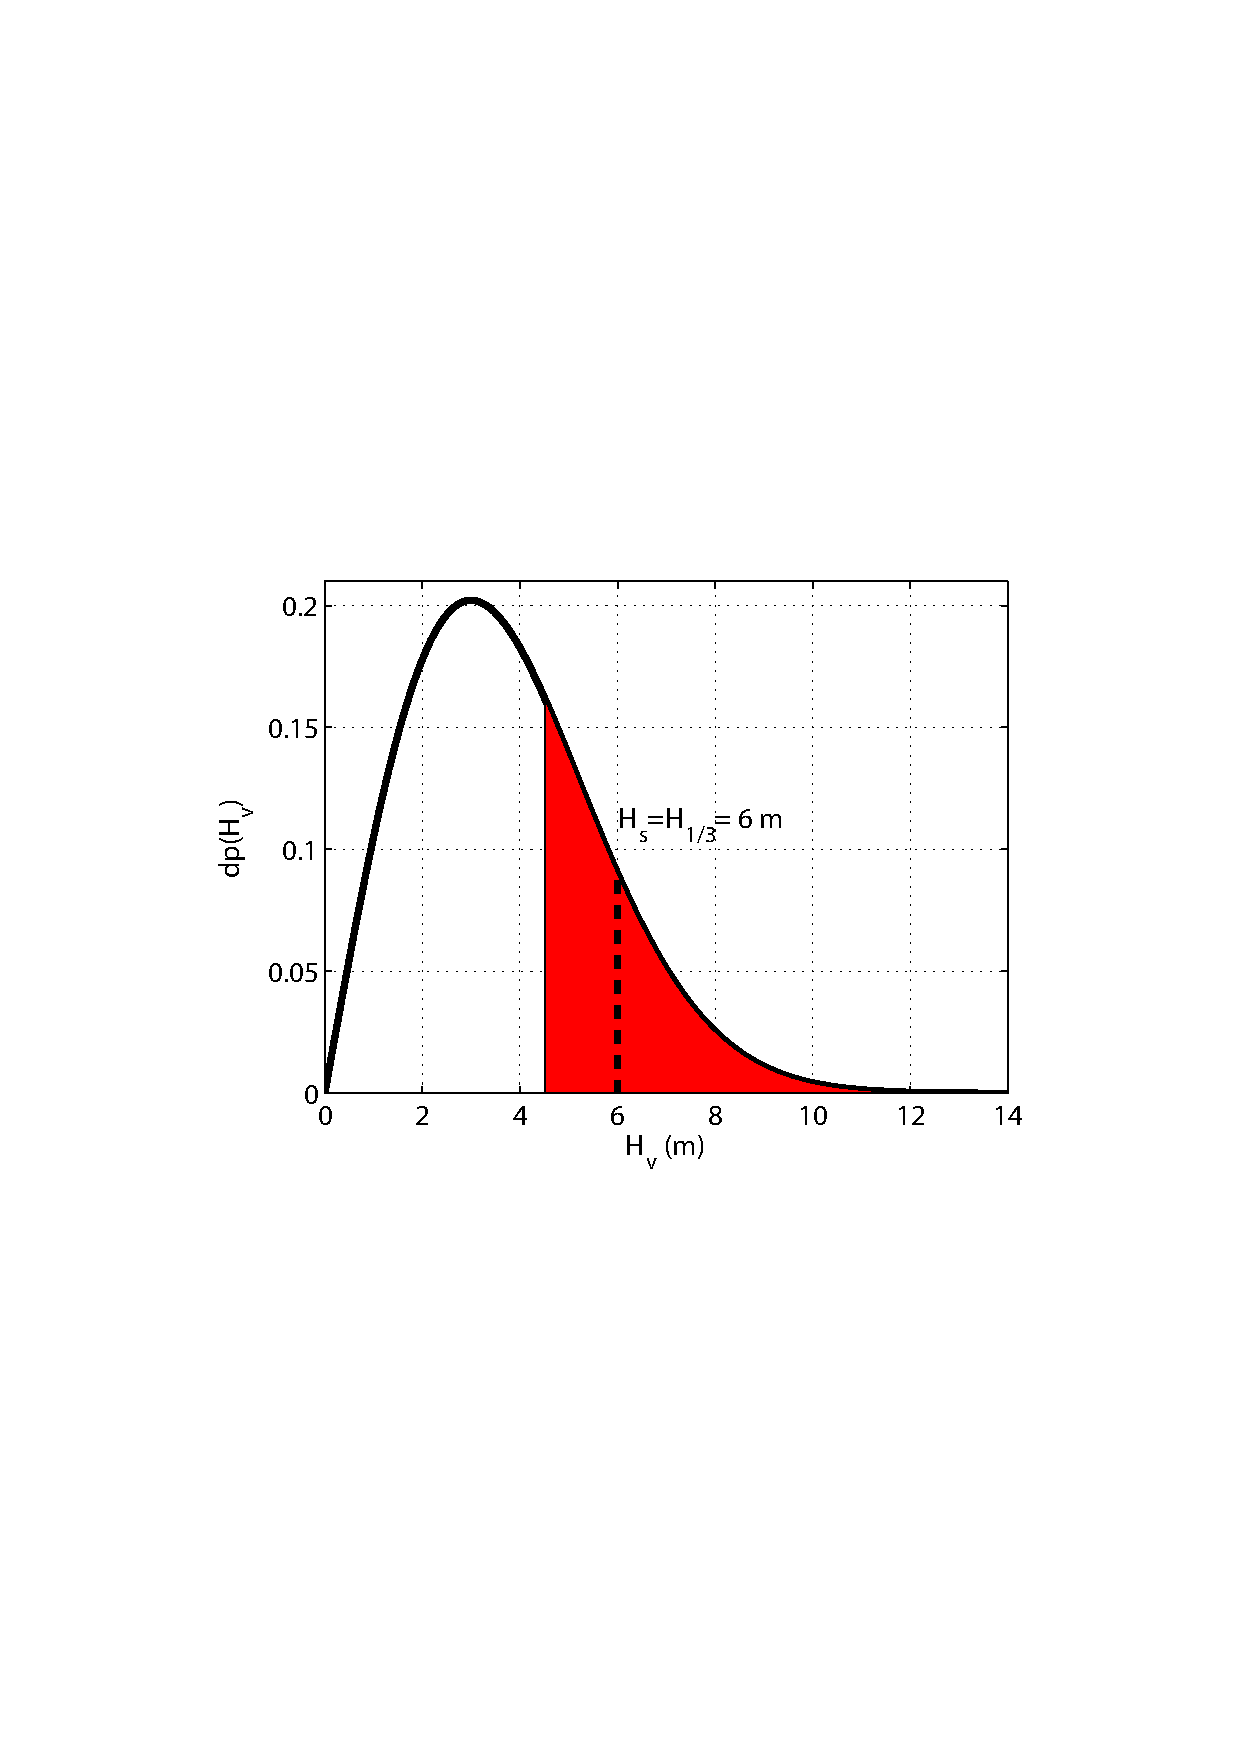
\includegraphics[width=0.6\textwidth]{FIGS_CH_INTRO/Rayleigh.pdf}}
%\vspace{3.64in}
  \caption{ Rayleigh distribution of wave heights}{$dp\times dH(H_v)$ is a probability for a single wave to have a height between  $H_v$ and $H_v+dH$. 
In red: the 1/3 of the highest waves in the distribution. The average height in this red part is $H_{1/3}$, which is one way to define the  significant wave height $H_s$. 
In the following chapters we will rather define $H_s$ as $H_{m0}$, equal to four times the standard deviation of the sea surface elevation. That other definition is 
recommended by the World Meteorological Organization and it gives a number 
very close to $H_{1/3}$.\label{fig:Rayleigh}}
\end{figure}
%%%%%%%%%%%%%%%%%%%%%%%%%%%%%%%%%%%%%%%%%%%%%%%%%%%%%%%%%%%%%%%%%%%%%%%%%%%%%

One useful result is that the probability that the height exceeds a given threshold $\widehat{H}$ 
is given by 
 \begin{equation}
P(H
>\widehat{H})=\er^{-\left(\widehat{H}/H_{\mathrm{rms}}\right)^2}\label{Hseuil}.
\end{equation}
This expression can be used to compute the height threshold $\widehat{H}$
associated to a fixed fraction of the wave population. For example 
$\widehat{H}_{1/3}$ is the height beyond which there are the highest 1/3 of the waves, and it is 
 $\widehat{H}_{1/3}=\left(\ln(3)\right)^{1/2}
H_{\mathrm{rms}}$ which is nearly 1.05$\times H_{\mathrm{rms}}$. 

A more commonly used scale for the wave heights is given by integrating 
 (\ref{Hseuil}) to get the average height of the 1/3 highest waves. This is one definition of 
the significant wave height, denoted $H_{1/3}$ or $H_s$. This scale roughly corresponds to the visual impression of wave heights, which was the most common source 
of measurements until the 1940s. 
More generally but still for a Rayleigh distribution, the average height of the $1/x$ fraction of the highest waves is, 
\begin{equation}
\left[\left(-\ln(1/x)\right)^{1/2} + \sqrt{\pi} \times
{\mathrm{erfc}}\left[\left(\ln(x)\right)^{1/2}\right]/2\right]
H_{\mathrm{rms}}
\end{equation}
 where erfc is the complementary error function.  For 
$x=1/3$, this gives $H_{1/3}=1.4157 \times H_{\mathrm{rms}}$.

From the definition, the full Rayleigh PDF $p(H)$ is determined by $H_{\mathrm{rms}}$. In practice the average $H_{1/3}$ is more 
commonly used, and there is also a lot of interest in the maximum height $H_{\mathrm{max}}$, but that one depends on the length of the 
record. When recording more waves,  $H_{\mathrm{max}}$ is likely to be higher. Waves that have a height
$H$ larger than $2.1 H_{1/3}$ are called freak waves or rogue waves. If we follow the Rayleigh statistics, 
this correspond to 1 in 5700 waves. In practice, they are a bit more frequent for conditions with large average steepnesses, as 
predicted by \cite{Tayfun1980}. Also, for real waves the spectrum is not always narrow and on average $H_{1/3} \simeq 3.8 \sqrt{m_0}$
instead of $H_{1/3} \approx 4.004 \sqrt{m_0}$, where $m_0$ is the variance of the surface elevation \citep{Goda1985}.

In the context of the design of coastal or oceanic structures,  there is a great interest in defining the 
maximum wave conditions that will occur over the expected lifetime of a structure, typically 50 to 100 years, 
or with a very low probability of occurrence to ensure maximum safety. For example, some sections of the Dutch dyke system
are required by law to resist waves that occur only once in 10,000 years. 
The material and size of the structure is then designed to withstand 
these extreme conditions. If the extreme wave height and period is overestimated, the cost of construction 
is higher than it could have been. If the conditions are underestimated, the structure is likely to fail in a time shorter
than the expected lifetime. This early failure happened for the first oil platforms built in the North Sea, in an age
when there were no routine wave measurements. 

For these extremes, the Rayleigh distribution does not hold, because the $H_s$ is itself a random variable on the 
scale of days to centuries. The extreme wave statistics on these long time scales are determined by the 
distribution of extreme meteorological event, or, in shallow water, the joint distribution of water levels (including 
the astronomical tide) with weather events. These long term statistics are clearly different from the short term statistics. 
For short term, the sea state was a superposition of many independent wave trains, and we could use the central limit theorem. 
For long terms, we first need to determine the distribution of the significant wave heights  $H_{s}$, and the probability 
that the height of a single wave exceeds $H_0$ is then the conditional 
probability $p(H > H_0  | H_s = H_{s0})$. The distribution of $H_s$ follows a generalized Pareto distribution, 
and the probability $p(H > H_0)$ is given by integrating the conditional probability over $H_{s0}$. 

Obviously, this requires stationary statistics. In some regions 
these statistics fluctuate with climatic patterns like the North Atlantic Oscillation, which particularly impacts
the wave heights on the European Atlantic coast, or the El Nino-Southern Oscillation  (ENSO) which has a strong 
impact on waves in the central Eastern Pacific or on the U.S. West coast \citep{Bromirski&al.2005}. 
As an example, Edward Thornton, a renown specialist of nearshore dynamics, was asked in 1996 to provide 
some consulting advice for the construction of a wastewater pipeline in Monterey Bay, Central California. 
Construction started in 1997 in the middle of a very strong El Nino, 
the hundred-year wave height, which had been properly evaluated by Ed Thornton, was exceeded 
and the half-ton rocks protecting the pipe were too small to stay in place and were dispersed by the waves. 
For such a strong El Nino event, the storm waves that caused the damage on the U.S. West Coast were normal. 
One should thus use statistics with caution. Defining extreme wave heights is also very challenging in tropical areas where
they are associated with hurricanes that have random tracks: a 20-year record of hurricane tracks generally does not contain 
all possible tracks, in particular the one of the next hurricane that will destroy this or that facility. 
Finally, there are also long-term trends associated with global change \citep[e.g.][]{Wang&Swail2002,Charles&al.2012}, 
especially in the Arctic where the trend in sea ice extent  is leading to higher wave heights and periods \citep{Stopa&al.2016b}. 

\subsection{Maps}
Wave statistics from time series cannot represent all wave properties. Some of these, such as the 
length of crests, are defined from the spatial 
patterns in the wave field. This parameter, although secondary to the wave height, gives information 
on the spatial coherence of wave-induced motions and is thus very important when navigating a seaway or designing 
a structure that may be wider than the crest length.
 
Just like we have defined heights and periods, heights and lengths $L$ can be defined 
in the case of waves propagating all in the same direction, say $x$. In that case, the crests are infinitely long in the other 
direction $y$. One important parameter is then the wave slope, defined from the ratio $H/L$. For sinusoidal waves, the maximum 
slope is $\pi H/ L$. 

Things get more complex when considering real waves that propagate in all directions. 
One can use the theory of random fields, developed by \cite{Adler1981}. In that theory, the crests are defined 
as subsets of the horizontal plane that are simply connected and that are above the mean sea level. Using this definition 
requires a bit of topology. In this context it becomes more difficult to associate a crest with a trough. 
There is a strong development of spatial statistics for ocean engineering and oceanography, thanks to the development 
of video measurement techniques \citep{Fedele&al.2009a}. 

\cleardoublepage
\chapter{Main properties of linear waves}\label{ch1b}
This chapter explains how and why water moves in waves, once the waves have been generated. 
A more logical sequence might have been to study the generation process of the waves first, but it is much more complex 
and can only be understood once one knows how the waves move. The properties exposed in this chapter
are independent of the generation mechanism, and thus common to all surface gravity waves, including tsunamis, ship wakes, and wind-generated waves. 

In order to make things simple, we consider a flat, non-deformable bottom 
located at $z=-h$, and periodic waves in both space and time. This may sound very restrictive, but waves at 
sea generally behave as if the bottom were locally flat, and the periodicity allows us to study elementary waves 
that are later superimposed thanks to the quasi-linear wave motion, with some possible non-linear corrections to better fit
the equations of motion. We will thus start with the linear wave theory of unidirectional and monochromatic 
waves that was first developed by  \cite{Airy1841}, and which is a good approximation for waves of small height in not-too-shallow water. 
These are the typical conditions found in swells for depths larger than 50~m or so. Swells are the waves generated by winds in remote storms. 
It is also instructive for the oceanographer to play the game of differences, and find the common traits and main differences 
between these swells, and the tidal waves in shallow water that take the form of  Kelvin waves. In fact, most 
of the wave properties derived here also apply to Kelvin waves. The main difference is the geostrophic balance along the crest of Kelvin waves 
that does not exist for shorter gravity waves for which the Coriolis force can be neglected for most properties. 


We will try here not to get carried away by mathematics, which are necessary to arrive at quantitative predictions.
Instead we will use the equations only as tools to help us reveal the wave motion in terms of forces, pressure and flow, which should 
help us navigate the many simplifying assumptions ot understand the role term. 

\section{Waves: a question of gravity, pressure, mass and vorticity}
Before jumping into equations, we should make a few mechanical remarks. 
There is a motion in and above waves because the crests and troughs of the sea surface, located at $z=\zeta(x,y,t)$, 
correspond to different weights of water, which 
creates a pressure difference. We can already note that these pressure variations 
are of the order of $\rho_w g \zeta$, with $\rho_w$ the water density and $g$ the vertical apparent\footnote{Apparent means that 
this is not just Newton's general gravitation but it also includes the centrifuge acceleration due to the Earth rotation, giving 
$g \simeq 9.81$m s$^{-2}$.} acceleration of gravity. With a 1~m difference in height from crest to trough, 
we get a pressure difference of 10 kPa. What is important for the motion is the pressure \emph{gradient}. With a wavelength 
of 200~m, this gives a crest-to-trough pressure gradient of the order of 100 Pa/m at the same level $z$, 
which drives a horizontal acceleration of 0.1~m/s$^2$. 

The water set in motion flows in an orderly way, following several principles. 
First, the mass of water is conserved, and for the slow velocities considered in this chapter, the flow is 
incompressible, hence non-divergent. We will also consider that the bottom does not deform under the waves. 
As a result, the horizontal convergence between a crest and the next trough must give 
rise to a vertical divergence. Besides, because the waves are generated by pressure forces, and propagated by pressure forces, 
the motion is, in a first approximation, irrotational. The vertical and horizontal velocities are thus strongly constrained by 
these two properties: \textbf{incompressibility} and \textbf{zero vorticity}.

In summary, the free surface position $\zeta$ and gravity determine the near-surface pressure $p$, which gives the horizontal velocity $u$. 
The vertical velocity $w$ is determined from the horizontal velocity using the 
zero divergence and vorticity conditions, and $w$ also modifies the pressure field. We thus can express 
the problem of wave mechanics as a set of four equations for the four unknowns that are $\zeta$, $p$, $u$ and $w$. 
%%%%%%%%%%%%%%%%%%%%%%%%%%%%%%%%%%%%%%%%%%%%%%%%%%%%%%%%%%%%%%%%%%%%%%%%%%%%%
\begin{figure}
\centerline{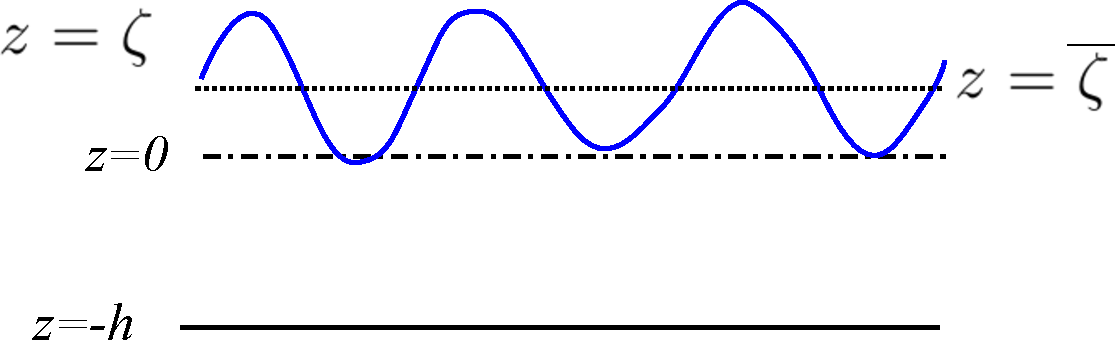
\includegraphics[width=0.5\textwidth]{FIGS_CH_AIRY/vertical_coord_def.pdf}}
%\vspace{3.64in}
  \caption{Definition of vertical levels: $\zeta$ is the sea level, $-h$ is the bottom, both defined relative to an arbitrary vertical datum $z=0$. As a result the
mean water depth is $D=h+\overline{\zeta}$.}
\label{fig:Dandh}
\end{figure}
%%%%%%%%%%%%%%%%%%%%%%%%%%%%%%%%%%%%%%%%%%%%%%%%%%%%%%%%%%%%%%%%%%%%%%%%%%%%%

\section{Wave mathematics}
We shall see that two important quantities, the wavelength $L$ and period $T$ are closely related 
for waves of small amplitude $a$. Here we define "small" to  mean that both the sea surface slope $ka$ and non-dimensional depth $a/D$ are small, 
where $k=2\upi/L$ is the wavenumber, and $D=h+\zb$, is the mean water depth. We remind the reader that $z=-h$
is the vertical position of the bottom, and $\zb$ is the mean sea surface elevation, both relative to an arbitrary datum 
$z=0$.

These small parameters $ka$ and $a/D$ will appear repeatedly in this book. Their ratio gives a third parameter, which is independent 
of the wave amplitude, and that will be very important for the wave kinematics, this is the 
\textbf{non-dimensional depth} $kD$.

We will now go into the details of the linear wave theory, first 
laid out by Airy in the 19th century. It has the great advantages of being  \textbf{linear}, hence any combination of the 
linear solution is also a solution of the equations of motion. More importantly, this linear model explains many of the waves properties, 
and is very accurate for swells in not-too-shallow water, and is not too far off for most wave properties, even for waves 
breaking in the surf zone.  

Let us make two final remarks before we get into the equations. 
First, the linear waves exist only on paper, as all monochromatic waves are unstable, with a development of this instability 
that is faster for higher waves. This aspect is discussed in more details in chapters \ref{ch_sourceterms} and Part 3. 
Monochromatic waves are an acceptable solution for short evolution times, at least a few periods, possibly much more. Second, 
the choice of the Eulerian framework for the equations of motion
is not a very good choice for the accuracy, as the linear Lagrangian theory 
is much more accurate than the Eulerian theory of Airy, because of the very simple balance between the pressure gradient and the 
fluid parcel acceleration.  
\cite{vonGerstner1809} did find an exact theory that exactly satisfies the condition $p=p_a$ at the free surface, 
but it has an non-zero vorticity, which must be compensated by a sheared current. 
The use of Lagrangian equations is unfortunately 
more complex, and this is the main reason why we do not use it here. It is interesting to note, that 
mass conservation is linear in an Eulerian framework, 
while momentum conservation is non-linear, but the opposite is true for a Lagrangian framework. 

\section{Eulerian equations for wave motion}
Our starting point is the conservation of mass and momentum applied to 
the ocean, with the former reduced to a zero divergence as we consider a constant density, which is 
true for the ocean within a few parts per thousand, and incompressible flow. 
The horizontal position is defined by the two-component vector 
${\mathbf x}=\left(x,y\right)$ and the vertical is $z$. The corresponding velocities are 
${\mathbf u}=\left(u,v\right)$ and $w$. Considering sea water as a perfect fluid, 
we apply the Navier-Stokes equations, 
\begin{equation}
    \frac{\partial {\mathbf u}}{\partial t}+{\mathbf u}\bcdot\bnabla{\mathbf u}
    + w \frac{\partial {\mathbf u}}{\partial z}
    =-\frac{1}{\rho_w} \bnabla p +
    \nu \left(\nabla^2 {\mathbf u}+\frac{\partial^2 u}{\partial z^2}\right),
    \label{NSxy}
\end{equation}
\begin{equation}
    \frac{\partial w}{\partial t}+{\mathbf u}\bcdot\bnabla w
    + w \frac{\partial w}{\partial z}
    =-g - \frac{1}{\rho_w} \frac{\partial p}{\partial z} +
    \nu \left(\nabla^2 w+\frac{\partial^2 w}{\partial z^2}\right),
    \label{NSz}
\end{equation}
\begin{equation}
\bnabla\bcdot{\mathbf u} + \frac{\partial w}{\partial z}=0,
\end{equation}
where $\bnabla$ is the horizontal gradient operator. We thus have \textbf{four scalar equations} since \ref{NSxy} has two horizontal components
for the \textbf{four unknowns} that are $u$, $v$,
 $w$ and $p$. Our problem will be well posed as soon as we define the boundary conditions, from the continuity of 
velocity and or stresses (pressure and shear stresses) and initial conditions. At the bottom, we only impose a free slip
 \begin{equation}
w=-{\mathbf u} \bcdot \bnabla h \quad \mbox{at} \quad
z=-h\left({\mathbf x}\right)
\end{equation}
which simplifies to $w=0$ because we chose $h$ to be constant

At the surface, we make the further hypothesis that for any horizontal position $\mathbf{x}$ there is only one value $z=\zeta$ 
of the free surface position (this excludes an overturning of the surface, as found in plunging breakers). 
The free surface is a material surface, which means that water parcels on the surface must stay on the surface. 
This can be expressed by the condition 
\begin{equation}
    \frac{\rm d}{dt}\left(z-\zeta\right)=
    w - {\mathbf u} \bcdot \bnabla \zeta -\frac{\partial \zeta }{\partial t}= 0
    \quad \mbox{at\ }\quad z=\zeta.\label{eq:skbc}
\end{equation}
An interpretation of this surface kinematic boundary condition 
is that the vertical motion 
${\partial \zeta }/{\partial t}$ is the combination of the vertical velocity 
$w$ and the horizontal advection of the water parcels sliding along the surface ${\mathbf u} \bcdot \bnabla \zeta$.

To that kinematic boundary condition we add the dynamic boundary condition that express the continuity of 
stresses at the air-sea interface. Neglecting the wind stress and surface tension, these reduce to a continuity of 
the pressure. In this chapter we will assume that the atmospheric pressure is takes the constant value  $p_a$,
\begin{equation}
    p=p_a\quad \mbox{at\ }\quad z=\zeta.
\end{equation}

We now assume irrotational motion, so that the velocity field 
is given by the gradient of a velocity potential 
$\phi$. Namely, $ {\mathbf u} = \bnabla \phi$ and $w={\partial
\phi}/{\partial z}$. In this and all our notations, the classical operators  (gradient
$\bnabla$, Laplacian $\Delta$ ...) are restricted to the horizontal 
plane, in order to simplify notations. This assumption of irrotational wave motion
is generally consistent with observations of real waves. Still, the vorticity can be 
very strong locally, for example in in the bottom and surface boundary layers
or just after a wave has broken. Also, in the presence of sheared currents, the wave motion always has 
some vorticity, and a weak vorticity also arises from the Earth rotation. 
%Il faut noter que cette condition n'est
%n\E9cessaire qu'\E0 un instant donn\E9: un mouvement initialement
%irrotationnel reste irrotationnel. 
We finally start off by neglecting the viscous terms in the Navier-Stokes equations. This is justified by the 
fact that any significant 
wave-induced motion has scales of velocity $U$ and length $L$ that are large enough to 
make the Reynolds number $UL/\nu$ of the order of  10$^4$ or more.

All the assumptions made above remove some real features in the wave motion. 
Real waves always have some vorticity, which is also linked to the viscosity 
effects in the boundary layers. A rigorous treatment of these effects is possible 
and will be discussed in other chapters. We are here looking for the most 
simple solution that will capture most of the important properties of real waves. 


Replacing velocities by gradients of $\phi$ in
(\ref{NSxy})--(\ref{NSz}) one arrives at
\begin{equation}
    \bnabla \left[\frac{\partial \phi}{\partial t}
    +\frac{1}{2}\left(
    \left|\bnabla \phi\right|^2
    +\left(\frac{\partial \phi}{\partial z}\right)^2
    \right)
    +\frac{p}{\rho_w}+gz \right]=0,
\end{equation}
and
\begin{equation}
    \frac{\partial}{\partial z} \left[\frac{\partial \phi}{\partial t}
    +\frac{1}{2}\left(
    \left|\bnabla \phi\right|^2
    +\left(\frac{\partial \phi}{\partial z}\right)^2
    \right)
    +\frac{p}{\rho_w}+gz \right]=0.\label{eq:NStoBer}
\end{equation}
These two equations establish that the term in brackets is not a function of position and can 
only be a function of time $\gamma(t)$, 
\begin{equation}
    \frac{\partial \phi}{\partial t}
    +\frac{1}{2}\left(
    \left|\bnabla \phi\right|^2
    +\left(\frac{\partial \phi}{\partial z}\right)^2
    \right)
    +\frac{p}{\rho_w}+gz =\gamma(t).\label{eq:Bernoulli}
\end{equation}

The other important equation given by the conservation of mass is linear, 
The mass conservation equation was already linear, 
\begin{equation}
\bnabla \bcdot {\mathbf u} + \frac{\partial w}{\partial z} =0
\end{equation}
and is equivalent to Laplace's equation for $\phi$
\begin{equation}
    \bnabla^2 \phi + \frac{\partial^2 \phi}{\partial z^2}=0,
    \quad \mbox{at\ }\quad -h\leq z \leq \zeta. \label{Laplace}
\end{equation}


\section{Small slope waves over a flat bottom: the Airy solution}
So far, we had only assumed an incompressible flow (assumption A1), zero viscosity (A2), 
irrotational motion (A3), a flat bottom (A4). 

% and a sinusoidal  et que
%le potentiel des vitesses varie spatialement comme une sinuso\EFde
%(H5). 

We shall now linearize the momentum equation (\ref{eq:Bernoulli}), assuming that the wave amplitude is small enough to 
neglect the non-linear terms. This is verified in chapter Part 3, provided that 
the wave amplitude $a$ is much less than the wavelength $L$ and $a$ is much less than the mean water depth $D$. 


This gives the linearized Bernoulli equation
\begin{equation}
    \frac{\partial \phi}{\partial t} \simeq 
       -\frac{p}{\rho_w}-g z + \gamma(t).\label{Bernoulli_lin}
\end{equation}
Assuming that waves are propagating \footnote{In the presence of standing waves, $\gamma(t)$ 
is an oscillating function of the order of $g a^2/L$, as derived by \cite{Miche1944d}.  \cite{Longuet-Higgins1950} further showed that this pressure field is actually an acoustic wave when the water compressibility is considered, which explains the generation of seismic and acoustic waves by ocean wind-generated waves.} at a speed $C$, the motion is periodic as a function of $x-C t$ and thus $\gamma(t)$ is a true constant, that can be determined from the dynamic boundary condition $p=\overline{p}_a$ at $z=\zeta$,
This gives the pressure as a function of the velocity potential, for $z< \zeta$, 
\begin{equation}
    p=\overline{p}_a -{\rho_w}g(z-\zeta) 
    -\rho_w \frac{\partial \phi}{\partial t}.\label{p_all}
\end{equation}
The Bernoulli equation states that the pressure is the hydrostatic pressure plus some correction 
due to the non-stationary motion. The static pressure term has been removed by the linearization. 

The linearized kinematic boundary condition, which expresses the continuity of velocities, reads
\begin{equation}
    w = \frac{\partial \phi }{\partial z} \simeq \frac{\partial \zeta}{\partial t}
    \quad \mbox{at\ }\quad z=\zeta,  \label{surface_lin}
\end{equation} which corresponds to a flat sea surface approximation. 
We can further approximate that the actual sea level is not too far from the mean sea level $z=\overline{\zeta}$. 


Finally, the bottom kinematic boundary condition becomes, 
\begin{equation}
    w=\frac{\partial \phi }{\partial z}=0 \quad \mbox{sur\ }\quad z=-h.  \label{bottom}
\end{equation}

Taking  $\partial (\ref{Bernoulli_lin} \textrm{~at z=}\zeta)/\partial t $
+$g\times$(\ref{surface_lin}) we eliminate the unknown $\zeta$, and obtain our 
wave equation 
\begin{equation}
  \frac{\partial^2{\phi}}{\partial{t^2}}+g\frac{\partial\phi}{\partial z}=0, \quad \mbox{at}
\quad  z=\overline{\zeta}. \label{surface 1}
\end{equation}

Equations (\ref{bottom})--(\ref{surface 1}) are the bottom and top boundary conditions for Laplace's equation. The 
set of equation  (\ref{Laplace})--(\ref{surface 1}) is
usually called the Euler equation. Its full non-linear form is given in Part 3. 
 
\subsection{Solution: Laplace equation and vertical profiles}
Since we have a linear wave equation, it is natural to solve it 
using the Fourier transform that gives us a full basis of solutions. Without loss of generality, 
we thus look for solutions of the form, 
\begin{equation}
    \phi=\Re \left(\widetilde{\phi}\left(z\right)
     \mathrm{e}^{\mathrm{i}{\mathbf k}\bcdot{\mathbf x} - \sigma t} \right),
    \label{phi1}
\end{equation}
where $\Re(x)$ is the real part of $x$. Replacing in Laplace's equation gives the Helmolz equation 
\begin{equation}
    -k^2 \widetilde{\phi}+\frac{\partial^2 \widetilde{\phi}}{\partial z^2}=0.
    \label{Helmholz}
\end{equation}
Any solution is thus the sum of two exponentials, which can be recombined in the form 
\begin{equation}
    \widetilde{\phi}(z)=A \cosh\left(kz+kh \right)
        + B \sinh\left(kz+kh \right).
\end{equation}
The bottom boundary condition imposes that $B=0$, and we thus only keep the first term,
\begin{equation}
    \widetilde{\phi}\left(z\right)=\Phi_0
    \frac{\cosh\left(kz+kh\right)}{\cosh\left(kD\right)}.
    \label{cosh}
\end{equation}

Considering that the amplitude of the vertical velocity $w=\partial \widetilde{\phi} / \partial z$ at the surface, where $z+h=D$,  is the radian frequency $\sigma$ times the elevation amplitude $a$, 
we have 
\begin{equation}
    | \Phi_0 |   k \sinh (kD) / \cosh (kD) = \sigma a.
\end{equation}
Hence, from Laplace's equation alone we get the orbital velocities. Wave motion has a maximum horizontal speed at the crest with a magnitude  $\sigma a / \tanh(kD)$, and in the direction 
of propagation. Because of the Laplace equation, when $kD >> 1$ the motion decays exponentially away from the surface over a typical distance that is $1/k=L/2\pi$.

%The only fact that the velocity potential is a solution to Laplace equation gives important analogies with many other waves but also other physical phenomena: electromagnetic waves are also surface waves with "skin effects" when considering high enough frequencies. 


\subsection{Solution: Momementum balance and dispersion relation}
Replacing $\phi$ by eq. (\ref{phi1}) using (\ref{cosh}) in the wave equation (\ref{surface 1}) gives  
\begin{equation}
    - \sigma^2 \Phi_0 +gk\tanh\left(kD\right)\Phi_0=0.
     \label{onde 1}
\end{equation}
This equation expresses the balance of forces between the horizontal pressure gradient which, just below the surface is 
is hydrostatic, with an amplitude  $\rho_w g a k$, and the horizontal acceleration, which has an amplitude  $\sigma^2 a / \tanh(kD)$. 
This is the dispersion relation for linear waves over a flat bottom, first given by \cite{Laplace1776}, 
\begin{equation}
    \sigma^2=g k \tanh\left(kD\right).
     \label{dispersion}
\end{equation}
As a result, where $D$ is reduced but $\sigma$ is constant, waves have a lower phase speed $C=\sigma/k$  for example near the shoreline. 
Contrary to a widespread misconception, this reduction of the phase speed has nothing to do with bottom friction.
in fact the wave orbital velocity increases, and in the Airy theory there is no dissipation of energy.




\subsection{Solution: polarization relations}
Having solved for the velocity potential, we can now link it back to the surface elevation using eq. (\ref{surface_lin}). 
Defining the phase of the free surface elevation, 
\begin{equation}
   \Theta={\mathbf
k}\bcdot{\mathbf x}-\sigma t+ \Theta_0, \label{eq:phase}
\end{equation}
 with $\Theta_0$ a constant between 0
et $2\pi$, eq. (\ref{surface_lin}) links the surface elevation amplitude $a$ and the amplitude $\Phi_{0}$ of the velocity potential at the surface 
\begin{equation}
    a={\mathrm i}\frac{\sigma}{g}\Phi_{0},\label{afromPhi0}
\end{equation}
the elevation, velocities and pressure of the \cite{Airy1841}\footnote{Although 
Laplace, Cauchy and Poisson gave all elements of this theory many years 
before Airy, the latter was the first to address the problem of a single propagating monochromatic 
wave train. Poisson solved several problems of greater complexity, including stationary waves 
and circular waves \citep{Craik2004}.} We thus have  the  following 
polarization relations that link the amplitudes and phase of all oscillating variables 
\begin{equation}
    \zeta-\overline{\zeta}=a \cos \Theta,\label{polzeta}
\end{equation}
and the velocity potential 
\begin{equation}
    \phi=  \frac{a}{k}\sigma
    \frac{\cosh\left(kz+kh\right)}{\sinh\left(kD\right)}
    \sin \Theta.
      \label{potentielcos}
\end{equation}
gives the velocity field
\begin{equation}
    \ub= a \frac{{\mathbf k}}{k}\sigma
    \frac{\cosh\left(kz+kh\right)}{\sinh\left(kD\right)}
    \cos \Theta,
      \label{vitesse}
\end{equation}
\begin{equation}
    w=a \sigma
    \frac{\sinh\left(kz+kh\right)}{\sinh\left(kD\right)}
    \sin \Theta. \label{eq:w}
\end{equation}
The pressure field is obtained from the linearized Bernoulli equation with the constant 
given by the dynamic surface boundary condition, as in eq. (\ref{p_all}), 
\begin{equation}
    p=\overline{p}^H+\rho_w g a
    \frac{\cosh\left(kz+kh\right)}{\cosh\left(kD\right)}
    \cos \Theta,
      \label{pression}
\end{equation}
where the hydrostatic pressure is $\overline{p}^H=-\rho_w g
(z-\zb)+\overline{p}_a$ with ${p}_a$ the atmospheric pressure. 
We also have




%et la fonction de courant
%\begin{equation}
%    \psi=  \frac{a}{k}\sigma
%    \frac{\sinh\left(kz+kH\right)}{\sinh\left(kD\right)}
%    \cos \left({\mathbf k}\bcdot{\mathbf x}-\sigma t + \Theta \right),
%      \label{vitesse}
%\end{equation}


We obtain the displacements of water particles by integrating the velocity field in 
time. To a first order of approximation (at first order in $\varepsilon=ka$),
we have the horizontal displacement
\begin{equation}
     \widetilde{\xi}_h = - a \frac{{\mathbf k}}{k}
    \frac{\cosh\left(kz+kh\right)}{\sinh\left(kD\right)}
    \sin \Theta,
      \label{xi1}
\end{equation} and the vertical displacement
\begin{equation}
    \widetilde{\xi}_3 =a
    \frac{\sinh\left(kz+kh\right)}{\sinh\left(kD\right)}
    \cos \Theta \label{xi3}.
\end{equation}
Because of the wave propagation, the water parcels spend more time under the crest, where the horizontal 
velocity is larger, than under the trough, where the velocity is weaker. As a result there is a net, order $(ka)^2$ drift in the direction 
of propagation, even for linear waves. This is a Stokes drift - it is also called the wave (pseudo)-momentum. Like the energy and the wave action, the Stokes 
drift is an intrinsic quadratic property 
of the wave field. This aspect is discussed in more details in chapter \ref{ch_momentum}. 

Eq. (\ref{dispersion})--(\ref{potentielcos}) are all approximate solutions corresponding to the Airy waves. \cite{Stokes1849} extended this Airy solution 
to take into account the non-linear terms of the full equation (see Part 3), which improves the agreement with observations.
In the deep ocean, all measurements confirm that waves are very nearly irrotational and well described
by the theories of Airy and Stokes
\citep[see for example ][]{Thornton&Kraphol1974,Herbers&al.1992}. The general solution can be expressed as a 
series in powers of 
$\varepsilon_1=ka$, which was shown to converge by \cite{Levi-Civita1925}. Many methods have been developed to 
obtain various numerical approximations of the exact solution.

\subsection{Physical interpretation}
The wave motion is maintained by the restoring force of gravity, which acts in quadrature to the velocity field, 
and thus always overshoots the equilibrium and creates crests where there were troughs. 
The acceleration induced by the pressure field feeds back into the pressure, and the motion \emph{is not} hydrostatic. 
Near the surface, the pressure is nearly hydrostatic (figure \ref{fig:puv1}). If the depth is large enough, 
at some level the vertical acceleration eventually cancels the pressure oscillations so that there is no 
significant motion at a depth much larger than the wavelength. This is typical of a surface wave, the motion decays exponentially 
from the surface, it is 'evanescent' or 'inhomogeneous'. 
%%%%%%%%%%%%%%%%%%%%%%%%%%%%%%%%%%%%%%%%%%%%%%%%%%%%%%%%%%%%%%%%%%%%%%%%%%%%%
\begin{figure}
\centerline{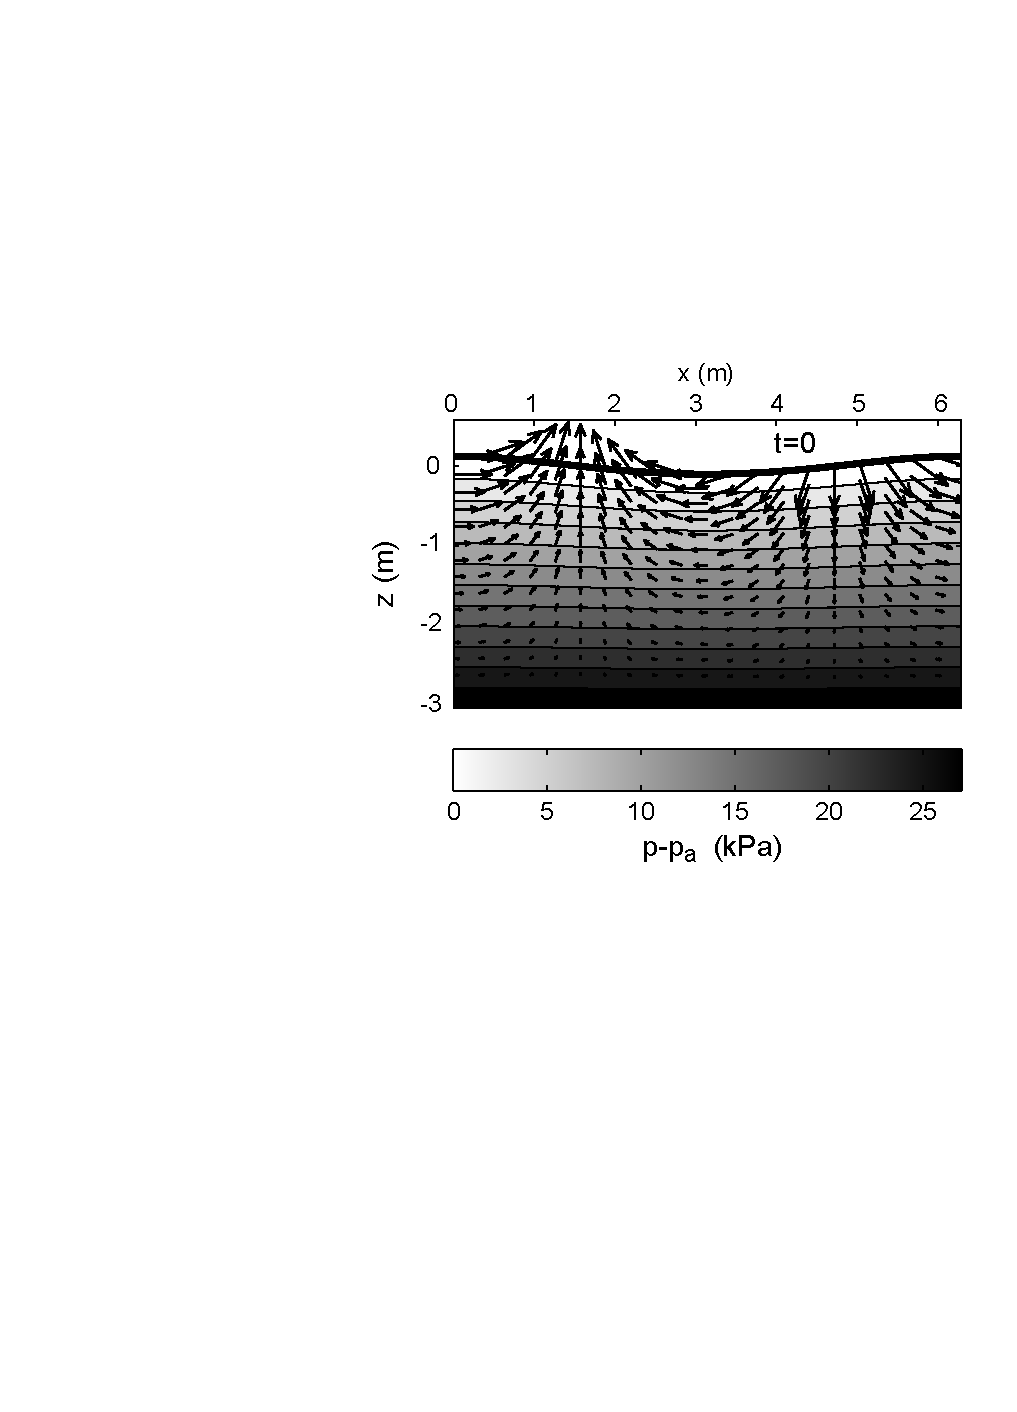
\includegraphics[width=0.6\textwidth]{FIGS_CH_AIRY/2sec_3mdepth_ppuv_1.pdf}}
%\vspace{3.64in}
  \caption{Pressure and velocity fields for a monochromatic wave of 
period $T=2$~s in a mean water depth of  $D=3$~m.}
\label{fig:puv1}
\end{figure}
%%%%%%%%%%%%%%%%%%%%%%%%%%%%%%%%%%%%%%%%%%%%%%%%%%%%%%%%%%%%%%%%%%%%%%%%%%%%%

The flow is better understood by looking at the pressure $p$ 
corrected for a hydrostatic pressure $p^H=p_a-\rho_w g (z-\overline{\zeta})$. This reveals a striking property, 
which is only true for $kD \gg 1$, the isobars of $p-p^H$ are also the streamlines. The streamfunction 
$\psi$ is such that $u=\partial \psi/\partial z$, which gives
\begin{equation}
    \psi=  \frac{a}{k}\sigma
    \frac{\sinh\left(kz+kD\right)}{\sinh\left(kD\right)}
    \cos \Theta,
      \label{potentiel}
\end{equation}
which is, for $kD\rightarrow \infty$ the pressure times $\rho_w g k$. 
This flow is in cyclostrophic equilibrium: the pressure gradient balances the 
centrifugal force of a water parcel turning around its circular orbit. 
%%%%%%%%%%%%%%%%%%%%%%%%%%%%%%%%%%%%%%%%%%%%%%%%%%%%%%%%%%%%%%%%%%%%%%%%%%%%%
\begin{figure}
\centerline{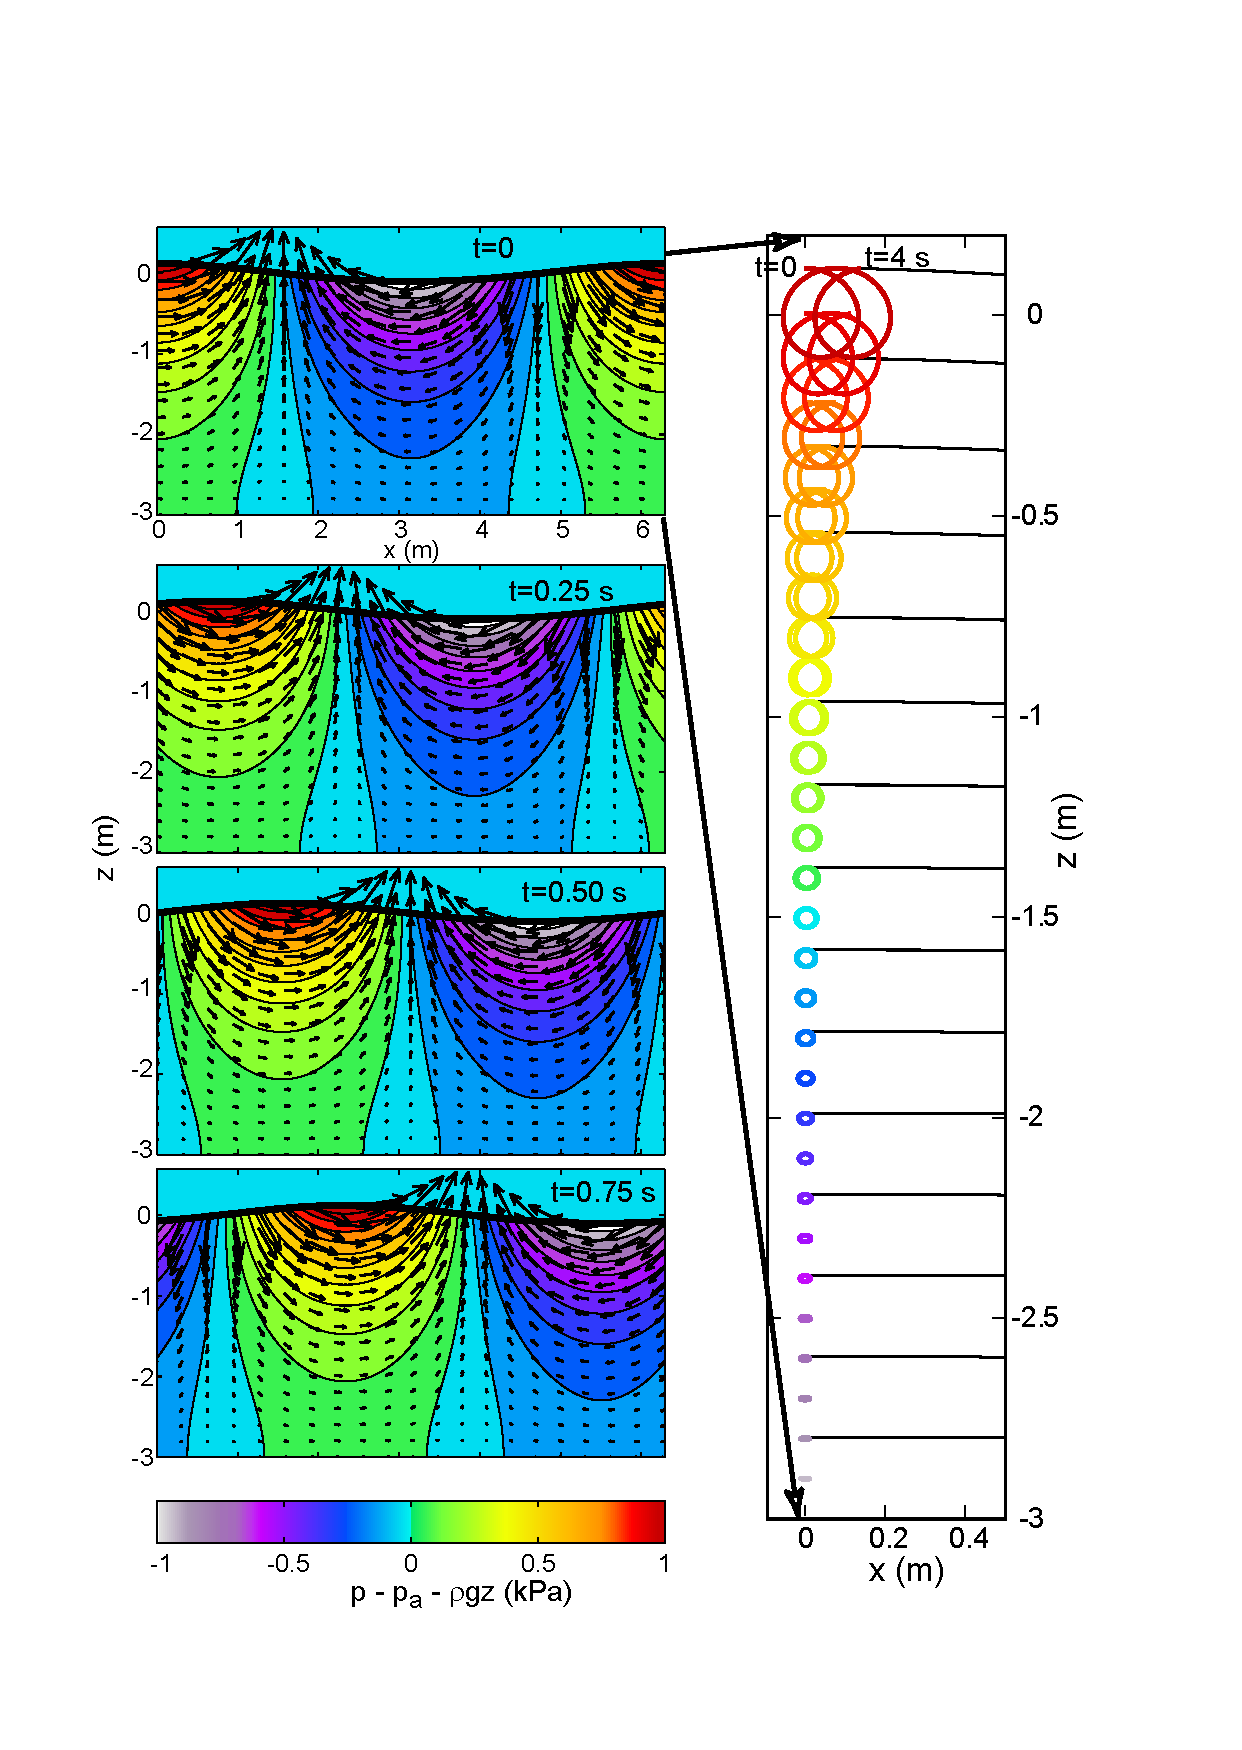
\includegraphics[width=0.9\textwidth]{FIGS_CH_AIRY/2sec_3mdepth_puv_drift.pdf}}
%\vspace{3.64in}
  \caption{Left, in colors: pressure anomaly $p-p^H$ and velocities at different phases 
of the propagation of 2~s period wave in 3~m water depth, going from left to right. 
Right: trajectories of water particles.}
\label{fig:puvdrift}
\end{figure}
%%%%%%%%%%%%%%%%%%%%%%%%%%%%%%%%%%%%%%%%%%%%%%%%%%%%%%%%%%%%%%%%%%%%%%%%%%%%%



%%%%%%%%%%%%%%%%%%%%%%%%%%%%%%%%%%%%%%%%%%%%%%%%%%%%%%%%%%%%%%%%%%%%%%%%%%%%%
\begin{figure}
\centerline{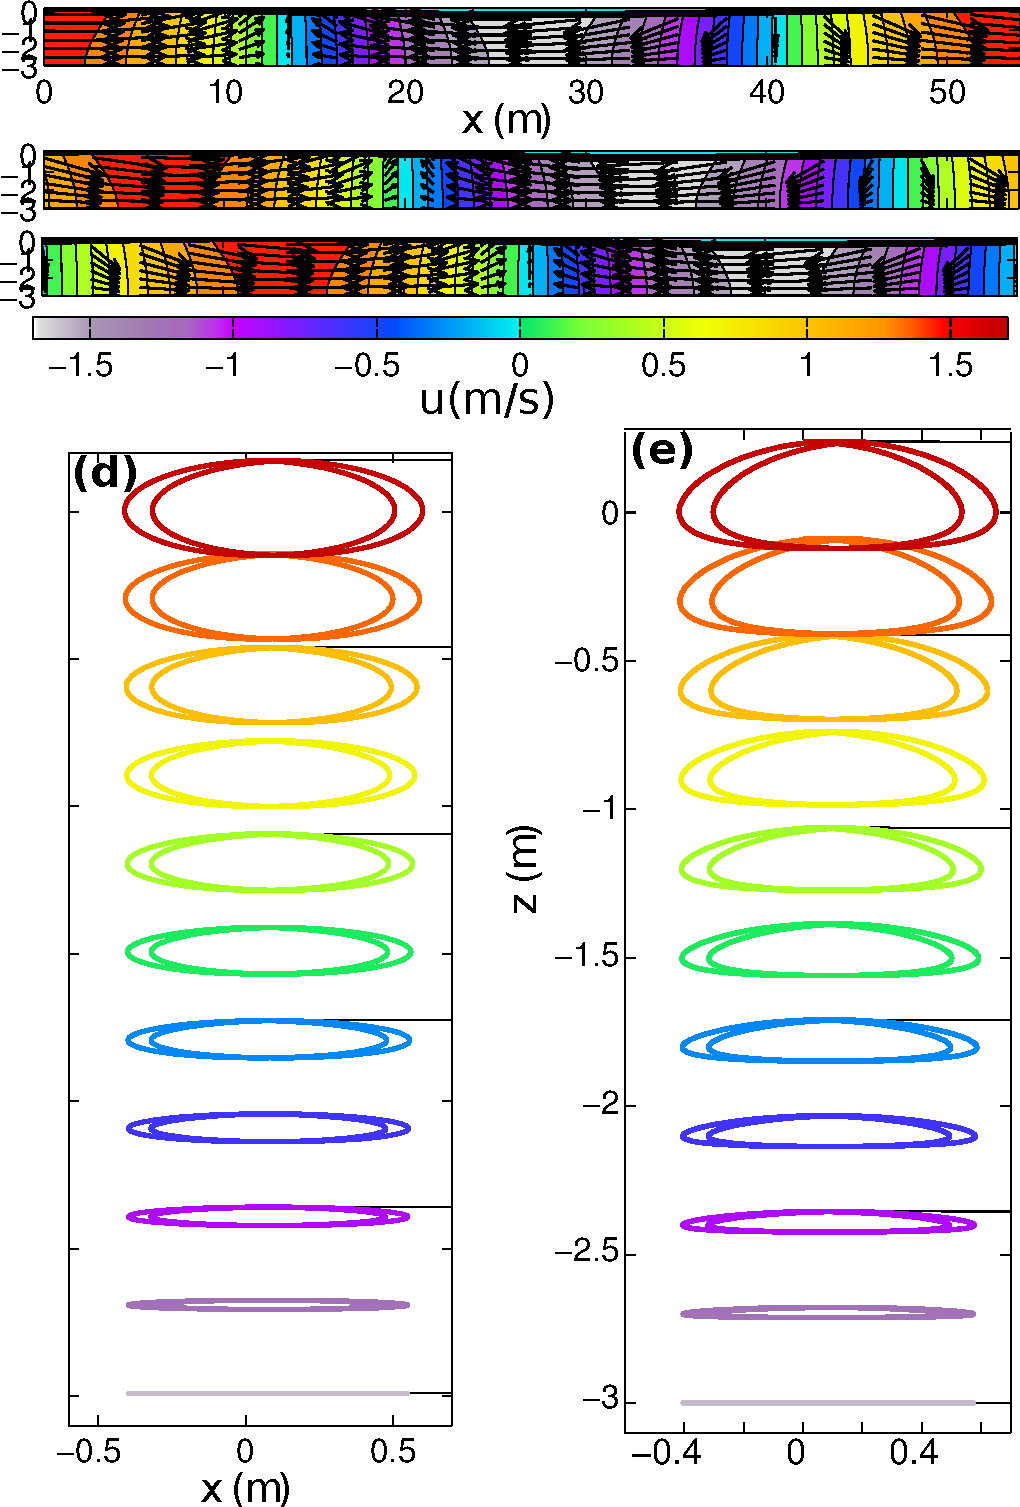
\includegraphics[width=0.7\textwidth]{FIGS_CH_AIRY/10sec_3mdepth_puv_drift.pdf}}
%\vspace{3.64in}
  \caption{Velocity field in water for a wave train of period 10~s, and amplitude 18~cm in 3~m of water. Snapshots are shown for 
(a) $T=0$, (b) 1.25 and (c) 2.5~s. 
The trajectories of water parcels are integrated over two Eulerian periods  (20~s) for (d) linear waves, and (e) nonlinear waves with the 
same period and height, using streamfunction theory (see part 3). For the height chosen here, $H/D=0.12$ and $H/L=0.0067$, so that 
linear theory gives a  fairly good approximation. }
\label{fig:uv2}
\end{figure}
%%%%%%%%%%%%%%%%%%%%%%%%%%%%%%%%%%%%%%%%%%%%%%%%%%%%%%%%%%%%%%%%%%%%%%%%%%%%%



\subsection{Kinematics: influence of the non-dimensional depth $kD$}
The changes in kinematics and dispersion from deep to shallow water are related to the hyperbolic functions $\cosh$, $\sinh$
and $\tanh$, which are plotted in figure \ref{coshsinh}.
%%%%%%%%%%%%%%%%%%%%%%%%%%%%%%%%%%%%%%%%%%%%%%%%%%%%%%%%%%%%%%%%%%%%%%%%%%%%%
\begin{figure}
\centerline{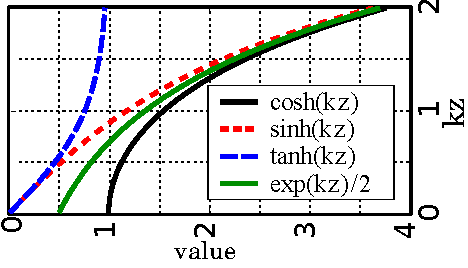
\includegraphics[width=0.5\textwidth]{FIGS_CH_AIRY/coshsinh_en.pdf}}
%\vspace{3.64in}
  \caption{The main hyperbolic functions, used again and again in ocean wave theory.}
\label{coshsinh}
\end{figure}
%%%%%%%%%%%%%%%%%%%%%%%%%%%%%%%%%%%%%%%%%%%%%%%%%%%%%%%%%%%%%%%%%%%%%%%%%%%%%


\subsubsection{Airy waves in deep water}
 A good number to remember is that, at a depth equal to half the
wavelength,  the motion amplitude is reduced by a factor $\exp(\pi) \simeq 25$ compared to the value at the surface.
As a result, waves such that $D > L/2$ which corresponds to $kD > \pi$, are generally considered to be 'deep water waves'.

The dispersion relation becomes, 
\begin{equation}
    \sigma^2 \simeq g k,
     \label{dispersion deep}
\end{equation}
the orbital velocities and pressures become
\begin{equation}
    \ub=a{\mathbf k}\frac{\sigma}{k}
    {\mathrm e}^{kz}    \cos \Theta
\end{equation}
\begin{equation}
    w=a \sigma
    {\mathrm e}^{kz}    \sin \Theta.
\end{equation}
\begin{equation}
    p=\overline{p}^H+ \rho_w g a
    {\mathrm e}^{kz}    \cos \Theta.
\end{equation}
and displacements (\ref{xi1})-(\ref{xi3}) are now
\begin{equation}
    \widetilde{\xi}_h=-a \frac{\mathbf k}{k}
    {\mathrm e}^{kz}  \sin \Theta,
\end{equation}
\begin{equation}
    \widetilde{\xi}_3= a {\mathrm e}^{kz}  \cos \Theta,
\end{equation}
which is the parametric equation of a circle of radius $a {\mathrm e}^{kz}$.
In first approximation, the water parcels follow circular orbits with diameters that vanish with deph. 
 
\subsubsection{Airy waves in intermediate water depth}
For smaller water depths, the orbital velocity is significant near the bottom 
and the trajectories are now ellipses with horizontal major axis measuring 
$2 a
{\cosh\left(kz+kh\right)}/{\sinh\left(kD\right)}$, and 
a vertical minor axis $2 a
{\sinh\left(kz+kh\right)}/{\sinh\left(kD\right)}$ that shrinks from $2a$ at the surface, 
to zero at the bottom where the motion is back and forth along the 
bottom.

In that range there is no asymptotic expression for the dispersion relation and one may use Table \ref{table_dispersion}. 

%%%%%%%%%%%%%%%%%%%%%%%%%%%%%%%%%%%%%%%%%
\begin{table}
  \centering
  \begin{tabular}{|cc  | cc | cc|}
\hline
    $Y=X\tanh(X)$ & $X$     & $Y=X\tanh(X)$ & $X$   & $Y=X\tanh(X)$ & $X$\\
 \hline
       0.05    &     0.2255   &     1.05 & 1.2414 &     2.05 & 2.1110	\\
       0.10    &     0.3216   &     1.10 & 1.2831 &     2.10 & 2.1570	\\
       0.15    &     0.3973   &     1.15 & 1.3249 &     2.15 & 2.2031	\\
       0.20    &     0.4627   &     1.20 & 1.3668 &     2.20 & 2.2495	\\
       0.25    &     0.5218   &     1.25 & 1.4088 &     2.25 & 2.2961	\\
       0.30    &     0.5767   &     1.30 & 1.4511 &     2.30 & 2.3428	\\
       0.35    &     0.6284   &     1.35 & 1.4934 &     2.35 & 2.3898	\\
       0.40    &     0.6778   &     1.40 & 1.5360 &     2.40 & 2.4370	\\
       0.45    &     0.7255   &     1.45 & 1.5788 &	2.45 & 2.4843	\\
       0.50    &     0.7717   &     1.50 & 1.6218 &	2.50 & 2.5318	\\
       0.55    &     0.8168   &     1.55 & 1.6651 &	2.55  &      2.5795   \\
       0.60    &     0.8611   &     1.60 & 1.7085 &	2.60  &      2.6273   \\
       0.65    &     0.9046   &     1.65 & 1.7523 &	2.65  &      2.6753   \\
       0.70    &     0.9476   &     1.70 & 1.7962 &	2.70  &      2.7234   \\
       0.75    &     0.9902   &     1.75 & 1.8405 &	2.75  &      2.7716   \\
       0.80    &     1.0324   &     1.80 & 1.8850 &	2.80  &      2.8200   \\
       0.85    &     1.0744   &     1.85 & 1.9297 &	2.85  &      2.8684   \\
       0.90    &     1.1163   &     1.90 & 1.9747 &	2.90  &      2.9170   \\
       0.95    &     1.1580   &     1.95 & 2.0199 &	2.95  &      2.9657   \\
       1.00    &     1.1997   &     2.00 & 2.0653 &	3.00  &      3.0145   \\
\hline
\end{tabular}
  \caption{Table of the inverse function of $X \tanh X$. Defining $Y=\sigma^2 D/g$ it gives $k=X/D$, 
which allows to invert the dispersion relation in the absence of current. 
For $Y< 0.05$ one should use $X=\sqrt{Y}$, and for $Y >3$ one should use $X=Y$. A more practical alternative is the Padé approxim}\label{table_dispersion}
\end{table}
%%%%%%%%%%%%%%%%%%%%%%%%%%%%%%%%%%%%


\subsubsection{Airy waves in shallow water}
For very shallow water  (say $kD < 0.1$), the dispersion relation 
becomes
\begin{equation}
    \sigma^2=g D  k^2,
     \label{dispersion shallow}
\end{equation}
and the velocities and pressure are 
\begin{equation}
    \ub=a{\mathbf k}\frac{\sigma}{k \sinh(k D)}
        \cos \Theta
\end{equation}
\begin{equation}
    w=a \sigma
    \frac{\left(kz+kh\right)}{\left(kD\right)}    \sin \Theta.
\end{equation}
\begin{equation}
    p=\overline{p}^H+ \rho_w g a     \cos \Theta = p^H.
\end{equation}
This last expression states that the pressure is hydrostatic, just like in 
tidal waves. Tsunamis also nearly follow this shallow water limit. 

 The orbital displacement (\ref{xi1})-(\ref{xi3})
are now
\begin{equation}
    \widetilde{\xi}_h=-a \frac{\mathbf k}{k \sinh(k D)}
    \sin \Theta,
\end{equation}
\begin{equation}
    \widetilde{\xi}_3= a \frac{\left(kz+kh\right)}{\left(kD\right)}  \cos \Theta,
\end{equation}

\subsection{And in the air?}
So far we have solved for the water motion. The same hypotheses of irrotational 
and incompressible flow will, in the air, produce the same equations and solutions. 
The only difference is that the bottom boundary condition is replaced by 
${\mathbf u}\rightarrow0$ as $z\rightarrow\infty$.
The air motion over waves is thus similar to the water motion in deep water waves. 
The air pressure oscillates, with an amplitude that decays exponentially 
with elevation. 
%%%%%%%%%%%%%%%%%%%%%%%%%%%%%%%%%%%%%%%%%%%%%%%%%%%%%%%%%%%%%%%%%%%%%%%%%%%%%
\begin{figure}
\centerline{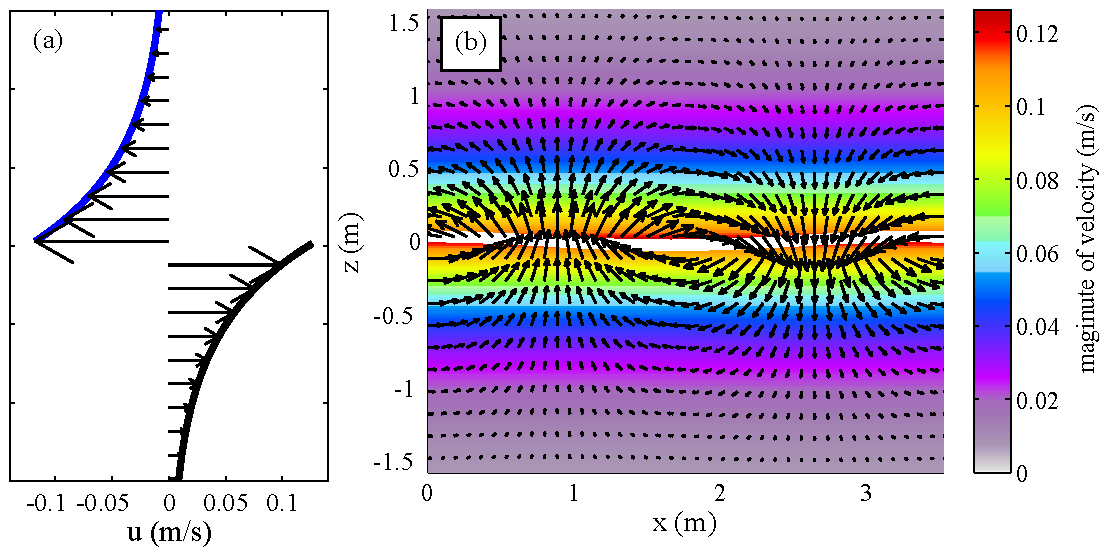
\includegraphics[width=\textwidth]{FIGS_CH_AIRY/vitesse_air_eau_en.pdf}}
%\vspace{3.64in}
  \caption{(a) Profile of the horizontal and vertical velocities on both sides 
of the sea surface at a wave crest ($x=0$), and (b) velocity field, with the white line indicating 
the position of the free surface. These velocities correspond to waves of amplitude $a=3$~cm, 
period $T=1.5$~s, in $D=3$~m water depth, which correspond to a wavelength 
$L=3.5$~m, and a non-dimensional water depth $kD=3.4$. }
\label{vitesse_air_eau}
\end{figure}
%%%%%%%%%%%%%%%%%%%%%%%%%%%%%%%%%%%%%%%%%%%%%%%%%%%%%%%%%%%%%%%%%%%%%%%%%%%%%

These results were confirmed by the measurements of \cite{Elliott1972a}, who 
found a vertical decay that is slightly faster than $\mathrm{e}^{-kz}$, due to 
the effect of the mean shear in the wind speed. When this shear is taken into account, the
Laplace equation is replaced by the Orr-Sommerfeld equation, as detailed in Part 3.
Besides, the velocity jump at the air-sea interface, gives rise to a boundary layer 
that is laminar for low wave heights and wind speeds \citep{Dore1978}, but becomes turbulent 
otherwise \citep{Perignon&al.2014}, probably leading to an important dissipation of long waves traveling across oceans that is 
discussed in Part 3.

\subsection{Dispersion}
The velocity at which the wave crests or trough propagate 
is called the phase speed and is given by $C=\sigma/k$ which is also equal to the ratio $L/T$. 
Using the dispersion relation (\ref{dispersion}), we can eliminate $\sigma$
\begin{equation}
    C= \frac{\sigma}{k}=\left[ \frac{g}{k}\tanh \left( kD\right)\right]^{1/2}.
\end{equation}
The phase speed is clearly a function of the wavelength, and thus waves are 
dispersive, meaning that wave packets that contain different components will 
spread over a larger space as they propagate, with the long waves traveling 
faster than the shorter waves. As a result, the waves arriving from a distant storm will 
always have a long period at the beginning and the average period will become shorter over time. 

This dispersion property disappears in shallow water  ($ kD << 1$)
where $C$ goes to $\left( gD\right)^{1/2}$, independently of $k$.
On figure \ref{disperlinLT}, this gives a constant slope, for example for $D=10$~m and $T>5$~s).
%%%%%%%%%%%%%%%%%%%%%%%%%%%%%%%%%%%%%%%%%%%%%%%%%%%%%%%%%%%%%%%%%%%%%%%%%%%%%
\begin{figure}
\centerline{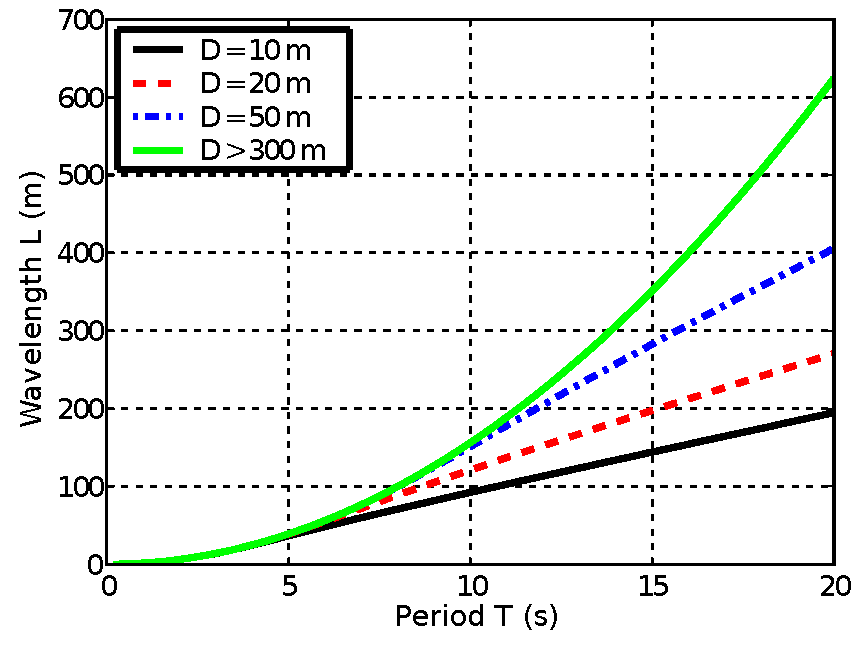
\includegraphics[width=0.8\textwidth]{FIGS_CH_AIRY/disperlinLT_en.pdf}}
%\vspace{3.64in}
  \caption{Wavelength as a function of the wave period and the water depth $D$, for linear waves in the 
absence of currents.}
\label{disperlinLT}
\end{figure}
%%%%%%%%%%%%%%%%%%%%%%%%%%%%%%%%%%%%%%%%%%%%%%%%%%%%%%%%%%%%%%%%%%%%%%%%%%%%%

We also note that, for a fixed period, the phase speed decreases 
with the water depth. This property is also true for a slowly varying water, 
in which case one can consider that the water depth is 'locally constant'. 
This variation of $C$ is the cause of refraction (see chapters \ref{ch_current} and \ref{ch5}). 


\subsection{Energy}
For any water particle, there is an oscillation of the kinetic and potential energies that are exchanged. 
Once integrated over the water depth and averaged over a wave period, that average is represented here by 
the overbar, the potential energy per unit horizontal surface is the vertical integral 
of the potential energy per unit volume $ \rho_w g z$. In practice, we ignore the constant energy between the 
bottom and the mean sea level $\overline{\zeta}$, and we set our reference level such that $\overline{\zeta}=0$,
\begin{eqnarray}
    E_p & = & \overline{ \int_{0}^{\zeta\left(\mathbf{x},t\right)} \rho_w g z {\mathrm d}z }
          = \rho_w g  \overline{ \frac{1}{2} \left(\zeta\right)^2 }   \nonumber\\
    & = & \frac{1}{2} \rho_w g a^2 \overline{ \cos^2\left({\mathbf k} \bcdot {\mathbf x}
    - \sigma t \right) } \nonumber\\
    & = & \frac{1}{4} \rho_w g a^2.
\end{eqnarray}
For the kinetic energy we integrate the kinetic energy per unit volume, $\left( \left|{\mathbf u}\right|^2 + w^2 \right)$ to obtain 
a kinetic energy per unit horizontal surface, 
\begin{eqnarray}
    E_c & = & \overline{  \int_{-h}^{\zeta\left(\mathbf{x},t\right)} \frac{1}{2} \rho_w
\left( \left|{\mathbf u}\right|^2 + w^2 \right) {\mathrm d}z } \nonumber\\
    & \approx & \frac{1}{2} \rho_w \left( \frac{a g k}{\sigma \cosh \left( kD \right)}
    \right)^2 \left[  \overline{ \cos^2 \Theta } \int_{-h}^{\zb} \cosh^2\left(kz+kh\right) {\mathrm d}z 
                   + \overline{ \sin^2 \Theta } \int_{-h}^{\zb} \sinh^2\left(kz+kh\right) {\mathrm d}z     \right] \nonumber\\
    & \approx & \frac{1}{4} \rho_w \left( \frac{a g k}{\sigma \cosh \left( kD \right)}
    \right)^2 \int_{-h}^{\zb} \cosh\left(2kz+2kh\right) {\mathrm d}z \nonumber \\
    & \approx & \frac{1}{4} \rho_w \left( \frac{a g k}{\sigma \cosh \left( kD \right)}
    \right)^2 \frac{\sinh 2kD}{2k}  \nonumber \\
    & \approx & \frac{1}{4} \rho_w g a^2,
\end{eqnarray}
\begin{equation}
    E_t= E_c+E_p= \frac{1}{2} \rho_w g a^2 = \rho_w g  E  ,\label{Etot}
\end{equation}
where $E$ is the variance of the sea surface elevation, here $E=a^2 /2$. 
We have thus found that, to a first order of approximation, the average kinetic and potential energy 
 $E_c$ and $E_p$ are equal. 

Wave propagation is associated to a flux of energy. This flux of energy is transmitted by pressure forces
from one water column to the next. This flux is the work 
of pressure forces given by eq. (\ref{pression}) with a velocity given by eq. (\ref{vitesse}). 
When integrated over the depth and averaged over a wave period, this gives the flux per unit crest length (i.e. per unit horizontal 
distance in the direction perpendicular to the propagation direction), 
\begin{eqnarray}
    W & = & \overline{ \int_{-h} ^{\zeta} p u \mathrm{d}z } \nonumber \\
        & = & \rho_w g a^2 \sigma
        \overline{ \cos^2\left({\mathbf k} \bcdot {\mathbf x} - \sigma t \right)  }
        \int_{-h} ^{\zeta} \frac{\cosh^2 \left(kz+kh \right)}{\sinh kD \cosh kD}
        ~ \mathrm{d}z \nonumber \\
        & = & E_t \frac{2  \sigma}{\sinh (2 kD)}
        \int_{-h}^{\zb} \frac{1}{2}\left[\cosh \left(2kz+2kh\right) +1 \right]
        \mathrm{d}z \nonumber \\
        & = & E_t \frac{2  \sigma}{\sinh (2 kD)}
        \left(\frac{\sinh 2kD}{4k}+\frac{D}{2} \right) \nonumber \\
        & = & C_g E_t \label{W}
\end{eqnarray}
where
\begin{equation}
C_g=\frac{\sigma}{k}
        \left(\frac{1}{2}+\frac{kD}{\sinh 2kD}\right)= C \left(\frac{1}{2}+\frac{kD}{\sinh 2kD}\right). \label{Cg}
\end{equation}
$W$ is a flux of energy per unit distance and $C_g$ the average speed at which the energy density $E_t$ is radiated, 
which defines the group speed. 

The full expression for the energy flux should also include the advective flux  $u \left[\rho_w g z + 0.5\left(u^2 +
w^2\right) \right]$, but that part is negligible in the absence of currents. 
%%%%%%%%%%%%%%%%%%%%%%%%%%%%%%%%%%%%%%%%%%%%%%%%%%%%%%%%%%%%%%%%%%%%%%%%%%%%%
\begin{figure}[htb]
\centerline{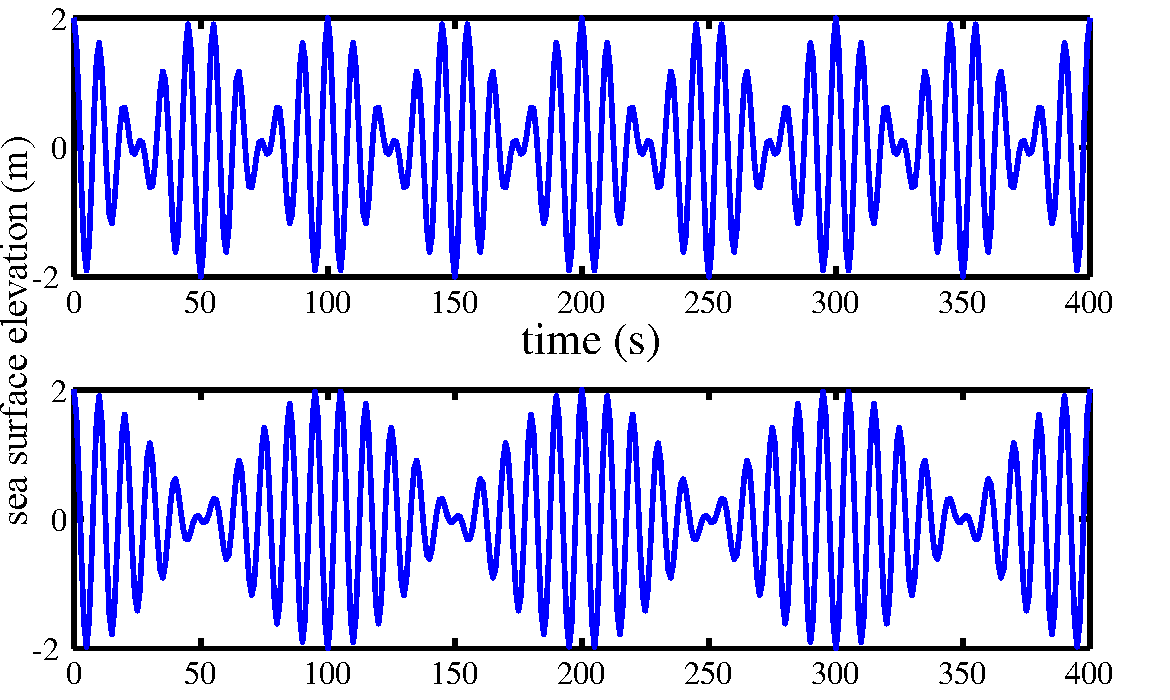
\includegraphics[width=0.7\textwidth]{FIGS_CH_AIRY/groups_5_10_en.pdf}}
%\vspace{3.64in}
  \caption{Wave groups produced by the superposition of two monochromatic waves. The top panel corresponds to  $\Delta \sigma/\sigma=0.2$, and the bottom panel
 $\Delta \sigma/\sigma=0.1$. The narrower the spectrum, the larger the number of waves in the group.}
\label{groupes}
\end{figure}
%%%%%%%%%%%%%%%%%%%%%%%%%%%%%%%%%%%%%%%%%%%%%%%%%%%%%%%%%%%%%%%%%%%%%%%%%%%%%

%%%%%%%%%%%%%%%%%%%%%%%%%%%%%%%%%%%%%%%%%%%%%%%%%%%%%%%%%%%%%%%%%%%%%%%%%%%%%
\begin{figure}
\centerline{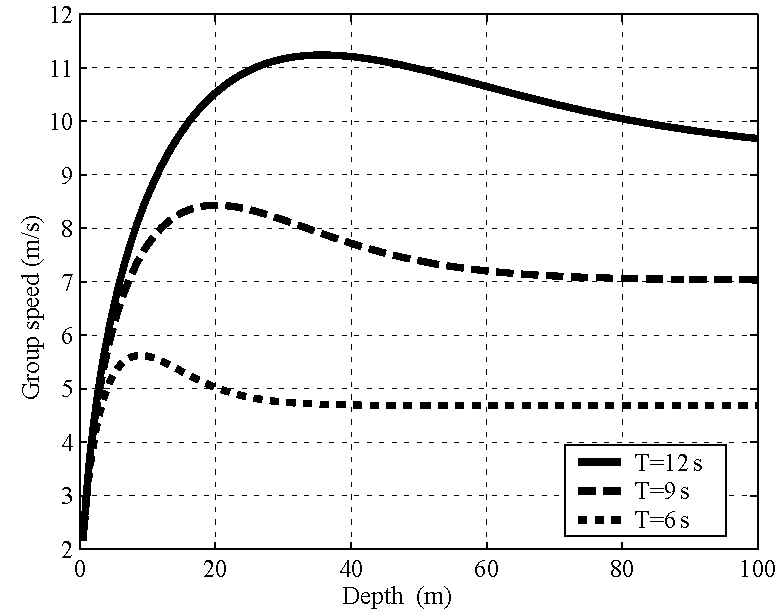
\includegraphics[width=0.55\textwidth]{FIGS_CH_AIRY/cg_en.pdf}}
%\vspace{3.64in}
  \caption{Group speed variation for different periods, as a function of the water depth.}
\label{Cgplot}
\end{figure}
%%%%%%%%%%%%%%%%%%%%%%%%%%%%%%%%%%%%%%%%%%%%%%%%%%%%%%%%%%%%%%%%%%%%%%%%%%%%%

This speed is called 'group speed' because it is indeed the speed at which a group of waves travels, because $C_g=\partial
\sigma/\partial k$. Indeed, the superposition of two monochromatic waves of equal amplitude and similar frequencies gives a surface elevation 
\begin{equation}
    \zeta=a  \cos \left[ \left(k - \Delta k \right) x - \left(\sigma-\Delta \sigma \right) t \right]
        + a  \cos \left[ \left(k + \Delta k \right) x - \left(\sigma+\Delta \sigma \right) t\right]  ,
\end{equation}
which writes
\begin{equation}
    \zeta=2 a \cos \left(\Delta k x -\Delta \sigma t\right)
    \cos \left( k x - \sigma t\right).
\end{equation}
The first factor is the envelope of the group, with a length  $2 \pi /
\Delta k $ and period $2\pi / \Delta \sigma$, that propagates at the speed 
$c'=\Delta \sigma /\Delta k $. This speed is, in the limit  $\Delta k \rightarrow 0$, equal to 
$C_g=\partial \sigma/\partial k$. Two examples are shown in figure 
\ref{groupes}.


We note that for $kD\rightarrow\infty$, equation (\ref{Cg}) gives
$C_g={\sigma}/({2k})=C/2$. Thus, in deep water the groups of waves travel at a speed that is half of the phase speed. 
Things are very different in shallow water ($kD
\ll 1$), where $C_g=C$. In that shallow water limit, waves of all frequencies travel at the same speed (they are not dispersive)
hence the groups also travel at that same speed. This is only true for linear waves. In part 3you may see that  phase and group speeds 
are also a function of the wave amplitude. 


\subsection{Energy and power}
Eq. (\ref{W}) gives the mean energy flux per unit crest length. 
For example, in the case of monochromatic waves with a height of 2~m, a period of 12~s and
a water depth of 15~m, this flux is 
$W\approx 50$~kW~m$^{-1}$. This means that if we take a surface facing the waves, 1 meter along the crest and the full water depth, there is 50~kW of mechanical power that goes through this surface. 
This is 5~MW for 100~m along the crests, which is the peak power of two  150~m high windmills. This number, for rather modest wave heights, 
shows the strong concentration of power in water waves. Unfortunately, this power is difficult to tap to produce electricity, in particular because it is very intermittent in most places.

\subsection{Summary}
We have obtained the main properties of regular linear waves,  summarized in table 
(\ref{table_theory}). Because these Airy waves are solutions of the linearized equations of motion, 
they can be combined to obtain the general solution. Hence the surface elevation, velocities and pressure 
are given by the sum of monochromatic waves, each proportional to their amplitude $a$. We will see in the next chapter that it is also possible to add up the quadratic properties 
that are the energy and Stokes drift, which are  proportional to the surface elevation variance
$E=a^2/2$.
%%%%%%%%%%%%%%%%%%%%%%%%%%%%%%%%%%%%%%%%%%%
\begin{table}
  \centering
  \begin{tabular}{lccc}
\hline
  Water depth: & general case       & $kD \gg 1$  & $kD \ll 1$  \\
\hline
  dispersion relation  &   $\sigma^2=g k \tanh (kD)  $               & $ \sigma^2=g k$ & $\sigma^2=g D k^2 $ \\
  phase speed & $C= {\sigma}/{k}=\left[g  \tanh (kD)/ k\right]^{1/2}$         & $C=\left(g / k\right)^{1/2} ={g}/{\sigma}  $   & $ C = \sqrt{gD}^{1/2}$ \\
  group speed  &  $C_g=C \left(0.5+\frac{kD}{\sinh(2kD)}\right)  $               & $C_g=C/2 $&
  $C_g=C$\\
\hline
  Linear properties  ($z<\zeta$) &    &  & \\
\hline
  horizontal velocity & $\ub =   a \frac{{\mathbf k}}{k}\sigma
    \frac{\cosh\left(kz+kh\right)}{\sinh\left(kD\right)}
    \cos \Theta $         &  $\ub=\frac{a \kb \sigma}{k} \er^{kz}    \cos \Theta$ & $\ub=\frac{a \kb \sigma}{k^2 D}
        \cos \Theta $\\
  vertical velocity & $w =   a \sigma
    \frac{\sinh\left(kz+kh\right)}{\sinh\left(kD\right)}
    \sin \Theta $         &  $w =a \sigma \er^{kz}    \sin \Theta$ & $w=\frac{z+h}{h}{a \sigma} \sin \Theta $\\
\hline
  Quadratic properties &    &  & \\
\hline
 Mean energy per unit surface & $E_t =  \rho_w g E = \rho_w g a^2 /2$  & $E_t =  \rho_w g  a^2 /2$ & $E_t =  \rho_w g  a^2 /2$ \\
 Stokes drift & ${\mathbf U}_s=\sigma \kb E \frac{\cosh(2kz+2kh)}{\sinh^2(kD)}$  & ${\mathbf U}_s=2 \sigma \kb E \er^{2kz} $ & ${\mathbf U}_s=\sigma \kb E /(kD)^2$ \\
\hline
\end{tabular}
  \caption{Main results of Airy wave theory with deep and shallow water limites.  We remind that the phase is  $\Theta={\mathbf
k}\bcdot{\mathbf x}-\sigma t+ \Theta_0$.
}\label{table_theory}
\end{table}
%%%%%%%%%%%%%%%%%%%%%%%%%%%%%%%%%%%%
These properties come from a series of assumptions, listed in table \ref{table_H} and that will be discussed or removed in 
the following chapters that extend Airy theory, giving access to all sorts of corrections and allowing to determine the 
evolution of Airy waves caused by different forcing and dissipation processes. Indeed, we have determined here the 
eigenvectors of the linearized equations of motion: these are free waves that can exist without forcing. In practice, the forcing 
is necessary to generate these waves in the first place, and this forcing is balanced by dissipation when long time scales and large 
spatial scales are considered. That dissipation requires to include vorticity and viscous effects. 
%%%%%%%%%%%%%%%%%%%%%%%%%%%%%%%%%%%%%%%%%%%
\begin{table}
  \centering
  \begin{tabular}{lcc}
\hline
 Assumption          & justification                                  & consequences  \\
\hline
 A1. incompressible &   $u \ll \alpha_w $             & $\bnabla \bcdot \ub + \partial w/\partial z=0$ \\
 A2. rigid bottom   & bottom motion $\ll$ water motion & $w=-\ub \bcdot \bnabla h$ at $z=-h$ \\
 A3. inviscid       & high Reynolds number                    & viscous stresses are zero \\
 A4. irrotational   & motion driven by pressure forces + (A3)   & $\ub=\bnabla \phi$, $w=\partial \phi/\partial z$\\
 A5. flat bottom    & bottom slopes usually $\ll$ 1 & with A2, $w=0$ at $z=-h$ \\
 A6. sine wave      & basis function of the Fourier transform & $\phi(z) \propto
 \cosh(kz+kh)$ \\
 A7. $p_a$ constant on $z=\zeta$ & $\rho_a \ll \rho_w$         &  no wave generation by the wind \\
 A8. no surface tension & $\gamma \ll g/k^2$ for $L \gg 0.1$~m (in clean water) & no capillary waves \\
 A9. $\varepsilon_1=ka \ll 1$ & $\varepsilon_1 <0.44$ for periodic waves & with A10, gives linear equations \\
 A10. $\varepsilon_2=a/D \ll 1$ & because it makes equations simpler & ... but beware for  $kD < 1$! \\
 A11. no mean current & most often $U \ll C$  for dominant waves & simple dispersion  $\sigma^2 = gk \tanh(kD)$ \\
 A12. constant density & $\rho'/\rho_w < 0.03$ for sea water   & no internal waves\\
 A13. no Earth rotation  & $f_3 \ll \sigma $          & \\
 \hline
\end{tabular}
  \caption{Assumptions needed to derive Airy's theory. $ \alpha_w$ is the sound speed in water, of the order of 
1500~m~s$^{-1}$ (in the absence of air bubbles), and $U$ is the mean current velocity. Finally $\rho'$ 
is a scale for density perturbations relative to the mean $\rho_w$, and 
 $\gamma$ is the surface tension, such that $\gamma \rho_w (R_1+R_2)$ is the additional pressure under a surface with radii of 
curvature $R_1$ et $R_2$, counted positive for a surface that is convex on the air-side, e.g. a crest.}\label{table_H}
\end{table}
%%%%%%%%%%%%%%%%%%%%%%%%%%%%%%%%%%%%

\subsection{Extending Airy wave theory}
What happens when we do not make one of the assumptions A1 to A13? In which conditions should we do this? 
\begin{itemize}
  \item A1. Except when considering acoustic and seismic noise generated by ocean waves, as in part 3, we can 
safely ignore compressibility effects. \vspace{0.3cm}
  \item A2. Bottom deformations are relevant when considering acoustic and seismic noise generation. In fact, the bottom 
deformation should be considered for all acoustic wave propagation in the ocean.  \vspace{0.3cm}
  \item A3. In the boundary layers at the sea surface, and more importantly at the sea bottom, 
we will need molecular viscosity and turbulence effects (which can often be represented by an eddy viscosity). 
However, these layers are very thin, with a thickness of the order of 
  $\delta=(\nu/\sigma)^{1/2}$, which is typically less than a millimeter for the kinematic viscosity of water 
$\nu \simeq 4\times 10^{-6}$~m$^2$~s$^{-1}$, and wave periods 
   $T > 1$~s, which is consistent with measurements of the water-side surface boundary layer by \cite{Banner&Peirson1998}. At the bottom, 
turbulence effects are important but the wave boundary layer is only a few centimeters thick.\vspace{0.3cm}
  \item A4. For a viscous flow, the vorticity from the top and bottom boundary layers diffuses in the water column 
and in the air \citep{Longuet-Higgins1953,Weber&Forland1990}. Besides, there is also a weak vorticity caused by the 
Earth rotation, see A13 below. \vspace{0.3cm}
  \item A5. The bottom boundary condition becomes $-\bnabla \phi \bcdot \bnabla h = \partial \phi/\partial z$ (inviscid case), 
and is only satisfied exactly in the presence of at least two wave trains, one incident and one reflected. The incident wave train 
is also modified by diffraction effects.
  For small slopes, diffraction and reflection are generally weak, 
and the wave motion is well approximated by a "WKBJ" approximation: replacing the phase  $\Theta$ by a function  $S(\xb,t)$ 
with $\kb=\bnabla S$ and $\sigma=-\partial S/\partial t$ (see chapter 
  \ref{ch5}). In this context \emph{small} means that refraction or diffraction effects do not produce of significant variation 
of the wave amplitude at the scale of one wavelength. A more accurate approximation of the dispersion relation 
over a sloping bottom was given by 
   \cite{Ehrenmark2005}, in the form 
   $\sigma^2=gk \tanh(kh \beta /\tan \beta)$, where $\beta$ is the angle between the bottom and the horizontal. This correction is 
weak, only 4\% for a slope $\beta=10^\circ$. For steep slopes, reflection becomes important and the separation of the 
variables $\xb$ and $z$ becomes meaningless. The velocity potential can be obtained numerically 
  \citep[e.g.][]{Athanassoulis&Belibassakis1999,Belibassakis&al.2001}.\vspace{0.3cm}
  \item A6. For a flat bottom this is not an assumption: we have the right to decompose the waves into sine waves because these 
are a complete basis. For small bottom slopes, the wave train is only \emph{locally} equivalent to a sine wave. 
For steep slopes, the wave train can suffer strong distortions at the scale of one wavelength \citep[e.g.][]{Magne&al.2007}.\vspace{0.3cm}
  \item A7. An atmospheric pressure oscillation on the scale of the wavelength can produce an amplification or attenuation of the waves, depending 
on its phase relative to the waves. This aspect is discussed in detail in chapters \ref{ch_sourceterms} and Part 3. \vspace{0.3cm}
  \item A8. Due to surface tension, the pressure under the surface is increased by  $-\gamma \left(\partial^2 \zeta/\partial x^2+\partial^2 \zeta/\partial
  y^2\right)$. This added pressure modifies the dispersion relation to give $\sigma^2=\left(gk+\gamma k^3\right) \tanh(kD)$. 
  This modification is negligible for wavelengths larger than a few centimeters. The presence of a layer of ice at the sea surface 
has a similar effect on the waves, with added terms due to bending and inertia, and is significant for periods of 10~s and 
less \citep{Liu&MolloChristensen1988} in the case of an ice layer thickness of one meter or more, and  thicker layers have an influence on longer waves.
  \item A9. Non-linear effects associated to $\varepsilon_1 \neq 0$ are fairly complex and will be 
discussed in chapters \ref{ch_sourceterms} and part 3. 
One particular consequence is that a monochromatic wave train is generally 
unstable \citep{Benjamin&Feir1967}. For waves in one dimension, as produced in the laboratory, 
this can create very high (freak) waves. Another consequence is that different wave trains interact, 
exchanging energy an momentum.\vspace{0.3cm}
 \item A10. Non-linear effects associated to  $\varepsilon_2 \neq 0$ are important for $kD<1$ even if the wave height is small. 
This is particularly true near the shoreline, and the shape of waves can be strongly modified, as discussed in chapters \ref{ch_surf} and 
part 3.\vspace{0.3cm}
 \item A11. Since the laws of physics are unchanged by a change of Galilean reference frame, 
a uniform current $\Ub$ in the absence of bottom friction only introduces a Doppler frequency shift, 
and all results established here remain valid, replacing 
$\Theta$ by $\Theta_D=\Theta+\kb \bcdot
 \Ub$. One can define an absolute frequency, as measured in the reference frame attached to the bottom, 
 \begin{equation}
    \omega=\sigma+\kb \bcdot \Ub =\kb \bcdot \Ub + \left[g k \tanh\left(kD\right)\right]^{1/2}.
     \label{dispersionD}
\end{equation}
For a current   $\Ub(z)$ that varies only in the vertical, and in the limit  $\varepsilon_1 \ll 1$  and $\varepsilon_2 \ll 1$, 
this dispersion relation generalizes to the form,
 \begin{equation}
    \omega\equiv\sigma+\kb \bcdot \Ub_A      \label{dispersionD2}
\end{equation}
with the advection speed given by \cite{Kirby&Chen1989}, 
 \begin{equation}
 \Ub_A   = \kb \bcdot \int_{-h}^{\zb} \Ub(z) \frac{2  k
\cosh\left[2k(z+h)\right]}{\sinh(2kD)} \dr z. \label{dispersionD3}
\end{equation}
Finally, when $\Ub$ also varies horizontally, the phase speed varies horizontally, so that refraction and diffraction effects 
appear, just like they do on a sloping bottom. These questions are addressed  in  chapter \ref{ch_current}.\vspace{0.3cm}
\item A12. When the ocean is stratified, due to a vertical variation of temperature and/or salinity, the Airy waves are the 'external mode' in a family of waves that also include internal waves. 
Because the equations of motion are weakly nonlinear, these different modes are coupled, with an exchange of energy between surface waves and internal waves 
\citep{Thorpe1966}. This aspect is still relatively unexplored  \citep{Osborne&Burch1980,Kudryavtsev1994}. This stratification can also be due to the 
presence of air bubbles near the surface or sediments near the bottom, with important consequences for the bottom boundary layer and wave dissipation. 
\citep[e.g.][]{Winterwerp2007,Styles&Glenn2000}.\vspace{0.3cm}
\item A13. Taking into account the Earth rotation with a vertical Coriolis parameter $f_3$, a very weak transversal velocity component $v$ appears, 
of the order  $f_3 u /\sigma$ and in phase with $w$.  This transversal component is important for the surface drift current
 \citep{Hasselmann1970,Xu&Bowen1994,Ardhuin&al.2004b,Rascle&Ardhuin2009}. In the case of wind-generated waves, 
  $f_3/\sigma$ is typically of the order of 10$^{-4}$, so that the effect on the wave kinematics and dispersion is not measurable. 
There is also a very weak deviation of the propagation direction of the waves \citep{Backus1962}. This is still true for tsunamis 
which have much larger periods than wind-waves, typically a few minutes up to 30 minutes. Airy wave theory thus also applies to tsunamis, as long as non-linear effects are 
weak. On the contrary, for motions with longer periods, such as tides, the Earth rotation must be taken into account. This is why these waves are called inertia-gravity waves. 
\end{itemize}



\cleardoublepage
\chapter{Wave heights and spectra: theory and measurement}\label{ch2}
A detailed knowledge of the wave motion in any location is often not required, 
one may rather be interested in the evolution of some wave properties on distances 
much larger than the wavelength.  A statistical approach is therefore preferred.
Note also, that even in a wave tank, waves are never strictly monochromatic.

The most common method to represent the random nature of waves is the spectral analysis. 
It owes its success to the dispersive nature of waves (different components travel at different speeds), and it was made practical by the 
development of computer sciences in the 1960s and to the elegant 
Fast Fourier Transform (FFT) algorithm.  Those curious to know how a spectrum can be calculated without a computer can read the amazing account 
of the rotating system  invented by  \cite{Barber&al.1946} with variable speed to read off different spectral components off a wave record printed on paper .

With the Fourier method, a record of wave elevation $\zeta(t)$ is decomposed into 
a superposition of sine waves, each with a particular period. If the record has the three dimensions, $\zeta(x,y,t)$ this decomposition can be 
done in frequency, wavelength and propagation direction. 
The phases of theses sine waves are generally random, namely, the phase of one component 
in one record and the next record are not correlated at all. The only slowly varying quantity 
is the spectral density, defined as the amount of elevation variance per unit spectral bandwidth. 
The procedure can be applied to other variables, not just the elevation: pressure, velocity ... 
This slow variation of the spectrum allows a numerical prediction of ocean wave spectra. 

\section{Frequency spectrum}
The spectral analysis that is applied to wave measurements is fairly different from the harmonic 
analysis which is used for studying tides. Tides are described as a sum of discrete components whose frequencies are very well known as 
they are associated with astronomical motions. For tides we thus have a finite set of frequencies at which the amplitude and phase 
can be determined with great accuracy. Waves are described as a the sum of a 
 many components with energy at \emph{all} frequencies. There is no gap in the wave spectrum, and the phases are completely random, uniformly 
distributed between 0 and $2 \pi$ while the amplitudes 
also have random fluctuations. The result of the spectral analysis is a wave spectrum that describes
the wave energy distribution as a function of frequency. The practical method used to compute wave 
spectra from time series of surface elevation or pressure is detailed in Chapter \ref{ch_anaspec}. 

%%%%%%%%%%%%%%%%%%%%%%%%%%%%%%%%%%%%%%%%%%%%%%%%%%%%%%%  % FIGS_CH_MEASUREMENTS
\begin{figure}[htb]
\centerline{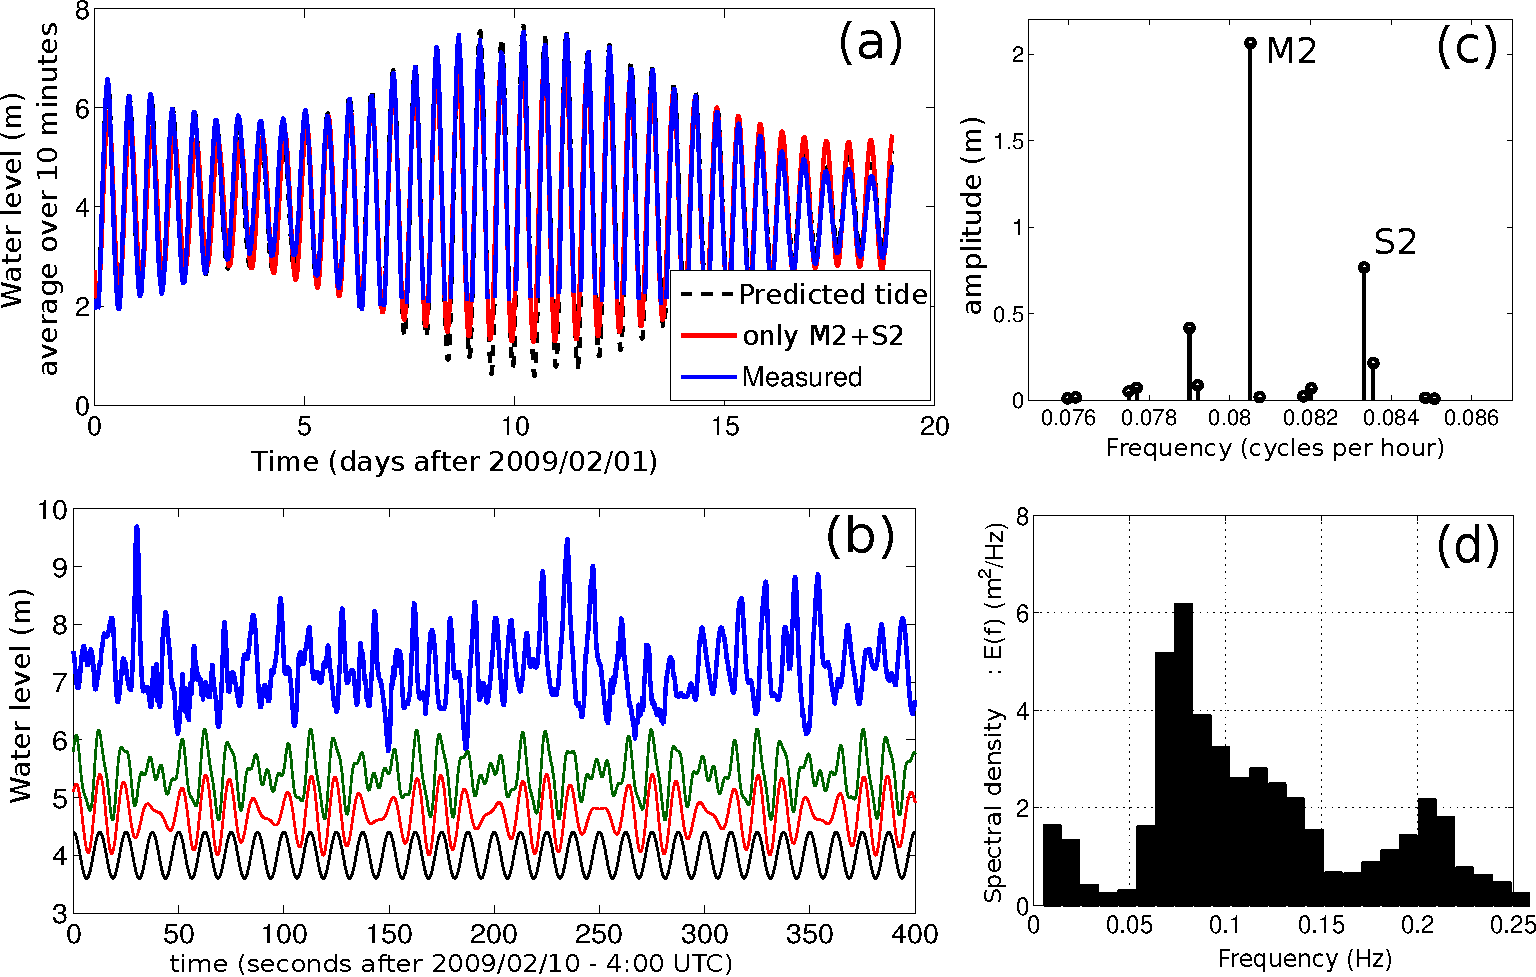
\includegraphics[width=\textwidth]{FIGS_CH_MEASUREMENTS/spectres_maree_vagues_en.pdf}}
%\vspace{3.64in}
  \caption{
Example of  surface elevation time series (a and b) deduced from pressure measurements collected 
as the foot of Western cliff of Banneg Island, Molene Archipelago. The corresponding spectra 
for the high and low frequency part illustrate the difference between a tide spectrum, 
presented as a function of amplitude and a wave spectrum. Below: a sample of the initial 
elevation signal and one, then two, then three sine waves are combined to approximate 
the initial signal. In the case of tides, the fit is already good with 2 components. In the case of 
waves, the detailed shape of the elevation cannot be reproduced without many components.}
\label{fig:maree_vagues}
\end{figure}
%%%%%%%%%%%%%%%%%%%%%%%%%%%%%%%%%%%%%%%%%%%%%%%%%%%%%%%%%%%%%%%%%%%%%%%%%
Figure \ref{fig:maree_vagues} shows how a tide elevation signal is already quite well 
reproduced by the superposition of only two sine waves (these two waves are called S2 and M2). 
On the contrary for the high frequency signal, dominated by waves, one, two or three sines 
waves (black, red and green) are far from sufficient for representing the initial signal (blue). 
Indeed, to reconstruct the wave signal a great number of sine waves with relatively close 
frequencies are required. For simplicity, let us start with one realization $m$ of an elevation 
time series, that can be expressed in terms of a Fourier series,
\begin{equation}
\zeta_{m}(t)=\sum_{i=1}^{N}a_{m,i}\cos(2\pi f_{i}t+ \Theta_{0,m,i})
\label{eq3.1}
\end{equation} 
Where $a_{m,i}$, $f_i$ and $\Theta_{0,m,i}$ are the Fourier amplitudes, frequencies and phases of 
the Fourier mode $i$, found for the realization $m$ of the sea state. As explained above, 
$N$ must be a large number. In practice the phases are nearly random and uniformly 
distributed over [$0,2\pi$] \footnote{The phases are not exactly random for an actual sea state, waves are 
slightly asymmetric, the front face being steeper than the back, and the crests sharper 
than troughs (e.g. \cite{Agnon&al.2005}). For most applications, these effects can be neglected.}. 
The ensemble mean of the Fourier amplitudes, expressed as function of the frequencies, 
 $A(f_i)= \left\langle a_{m,i}\right\rangle$ is called the amplitude spectrum.  For waves, 
identical sea state realizations can only be obtained in controlled laboratory experiments. 
Instead, the sea state is assumed stationary and the ergodicity theorem is evoked to replace the 
ensemble mean by a temporal mean. In practice, $M$ samples of a given (stationary) wave record simulate $M$ 
realizations of the sea state and provide an equivalent ensemble mean. 

For such random signals, the 'power' spectrum is preferred to the amplitude spectrum. 
As demonstrated in the previous chapter, the mechanical wave energy per unit surface of ocean, 
for an sine wave of amplitude $a$ is $\rho_w g a^2/2$. As a consequence, the energy spectrum is
\begin{equation}
\left\langle\frac{1}{2}a_{m,i}^{2}\right\rangle =\frac{1}{M}\sum_{m=1}^{M}\frac{1}{2}a_{m,i}^{2},
\label{eq3.2}
\end{equation}

With this definition, the values taken by the spectrum decrease proportionally to the spectral resolution $\Delta f$ that is the inverse of the length of time 
over which the spectral analysis is performed.  In order to avoid this dependency on the record length, it is customary to work with a power spectral density (PSD for short),
\begin{equation}
E(f_i)=\frac{1}{\Delta f} \left\langle \frac{1}{2} a_{m,i}^{2}\right\rangle. 
\label{eq3.3}
\end{equation}

In the limit of large record lengths, the frequency interval $\Delta f$ tends towards zero, and we obtain the continuous
wave energy frequency spectrum,
\begin{equation}
E(f)=\lim_{\Delta f\to 0}\frac{1}{\Delta f} \left\langle \frac{1}{2} a_{i}^{2}\right\rangle.
\label{eq3.4}
\end{equation}
 
While wave are irregular, the spectrum is relatively smooth, evolving slowly in space and time, with a typical time scale of a few hours. This regularity 
that contrasts with the apparent irregular motion of the sea surface, allows for a predictive numerical modeling. Note further, that
for convenience we continue to call (abusively) 'energy' the elevation variance $E$ which has units of length squared. 
The true energy, in Joules per unit surface, is in fact $\rho_w g E$. 

 This approach can be generalized to waves travelling in all directions. The Fourier representation of the sea surface elevation becomes,  
\begin{equation}
\zeta_m(x,y,t)=\sum_{i=1}^{N} \sum_{j=1}^{M}a_{m,i,j}\cos(2\pi f_{i}t- k_{i}\cos(\theta_{j}) x - k_{i}\sin(\theta_{j}) y + \Theta_{0,m,i,j}),
\label{eq3.5}
\end{equation}
as illustrated by figure \ref{fig:sumofsinewaves}
 %%%%%%%%%%%%%%%%%%%%%%%%%%%%%%%%%%%%%%%%%%%%%%%%%%%%%%%%%%%%%%%%%%%%%%%%%%%%%
\begin{figure}[!htbp]
\centerline{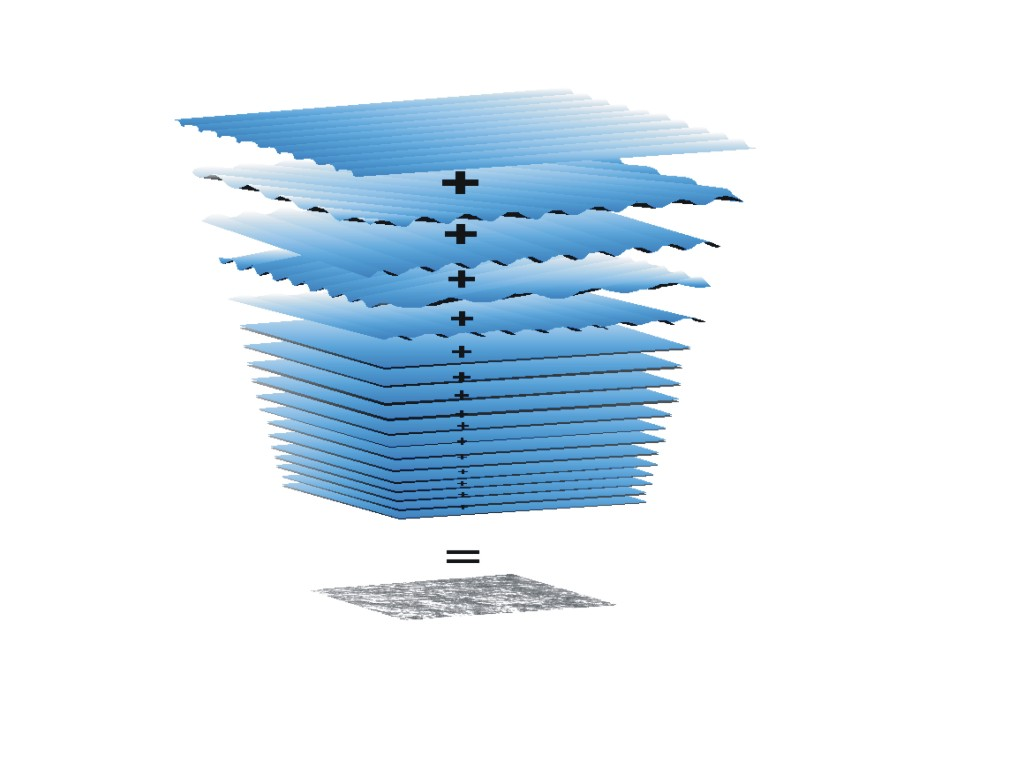
\includegraphics[width=0.8\textwidth]{FIGS_CH_MEASUREMENTS/Pierson1952.jpg}}
\caption{Reconstruction of a given sea state from the superposition of a great number of plane waves each with a particular direction and wavelength. Illustration of equation \ref{eq3.5}. 
After \cite{Pierson&al.1955}.\label{fig:sumofsinewaves}}
\end{figure}
 %%%%%%%%%%%%%%%%%%%%%%%%%%%%%%%%%%%%%%%%%%%%%%%%%%%%%%%%%%%%%%%%%%%%%%%%%%%%%

In this expression $k_{i}$ and $f_i$ are related by the linear dispersion relation and $\theta_{j}$ is the direction of
propagation of the Fourier mode ($i$,$j$). In the same fashion as for the frequency, the continuous frequency-direction wave energy
density spectrum, 
\begin{equation}
E(f,\theta)=\lim_{\Delta f\to 0}\lim_{\Delta \theta\to 0}\frac{1}{\Delta f \Delta \theta} \left\langle \frac{1}{2} \rho_w g a_{i,j}^{2}\right\rangle .
\label{eq3.6}
\end{equation}

Obviously, $E(f,\theta)$ is just a redistribution of $E(f)$ on the different wave directions and we recover the heave spectrum by summing on these directions, 
\begin{equation}
E(f) = \int_{0}^{2\pi}  E(f,\theta)d\theta.
\label{eq3.16}
\end{equation}

Keeping only the wave energy and its distribution reduces the   representation of the waves properties to a manageable amount of information, 
but some information is lost in the 
process. Indeed, it is not possible to reconstruct the sea surface from the spectrum, especially because the phases  are not conserved. 
In practice, the phase couplings are often negligible, and any reconstructed sea surface with 
random phases is statistically similar to the initial wave field. In this sense, for a Gaussian sea surface elevation, the spectrum contains 
the full statistics of the sea surface.

 \subsection{Wavenumber or frequency?}
 Depending on the measurement method, the numerical model or the application, one may want to perform the spectral analysis in the wavenumber or
 frequency space. The following relations between the frequency and wavenumber spaces, assume that waves follow the linear
 dispersion relation. The rule is simple, the variance of a given quantity does not depend on the coordinates in spectral space. 
The  variance is the spectral density times the spectral width, hence,
 \begin{equation}
E(f,\theta)d\theta df = E(k,\theta)d\theta dk 
\label{eq:Eftheta_Ektheta1}
\end{equation}
 which yields
 \begin{equation}
E(f,\theta)=\frac{\partial k}{\partial f} E(k,\theta) = \frac{2\pi}{C_g} E(k,\theta)
\label{eq:Eftheta_Ektheta}
\end{equation}

 In the same manner, 
 \begin{equation}
E(f,\theta)= \frac{2\pi}{C_g} E(k,\theta)= \frac{2\pi}{C_g}k E(k_{x},k_{y}) %=k\cos(f,k_{y})  CORRECT THIS !!!
\label{eq:Eftheta_Ekxky}
\end{equation}

The relationship must be used with caution for the high frequency part of the spectrum, because of nonlinear harmonics. This is significant at frequencies higher than three times the wind sea peak frequency \citep{Leckler&al.2015,Peureux&al.2018}. 
Finally, and we shall see why in chapter \ref{ch_courant}, when the effects of currents on  waves are included, numerical models 
usually work with the action spectrum instead of the energy spectrum. This action spectrum is usually defined as 
 \begin{equation}
A(k,\theta)=\frac{1}{\sigma}E(k,\theta)=\frac{1}{\sigma}E(k_{x},k_{y})
\label{eq3.10}
\end{equation}
For instance, the numerical model WAVEWATCH III \citep{Tolman&Booij1998} calculates the evolution of $A(k,\theta)$ discretized over
 $N$ frequencies and $M$ directions, through the variable ASPEC(I,J) with $1 \leq I \leq N $ and $1 \leq J \leq M $. However, 
the model output is transformed back to $E(f,\theta)$.
 

%  \subsection{Some spectra}
 The spectrum is the primary variable of wave forecasting model, and, as such, it is important to be familiar with its physical meaning. 
 Figure \ref{fig:spectres101}
 illustrates the relation between the sea surface and spectrum shapes.
%%%%%%%%%%%%%%%%%%%%%%%%%%%%%%%%%%%%%%%%%%%%%%%%%%%%%%%%%%%%%%%%%%%%%%%%%%%%%
\begin{figure}[!htbp]
\centerline{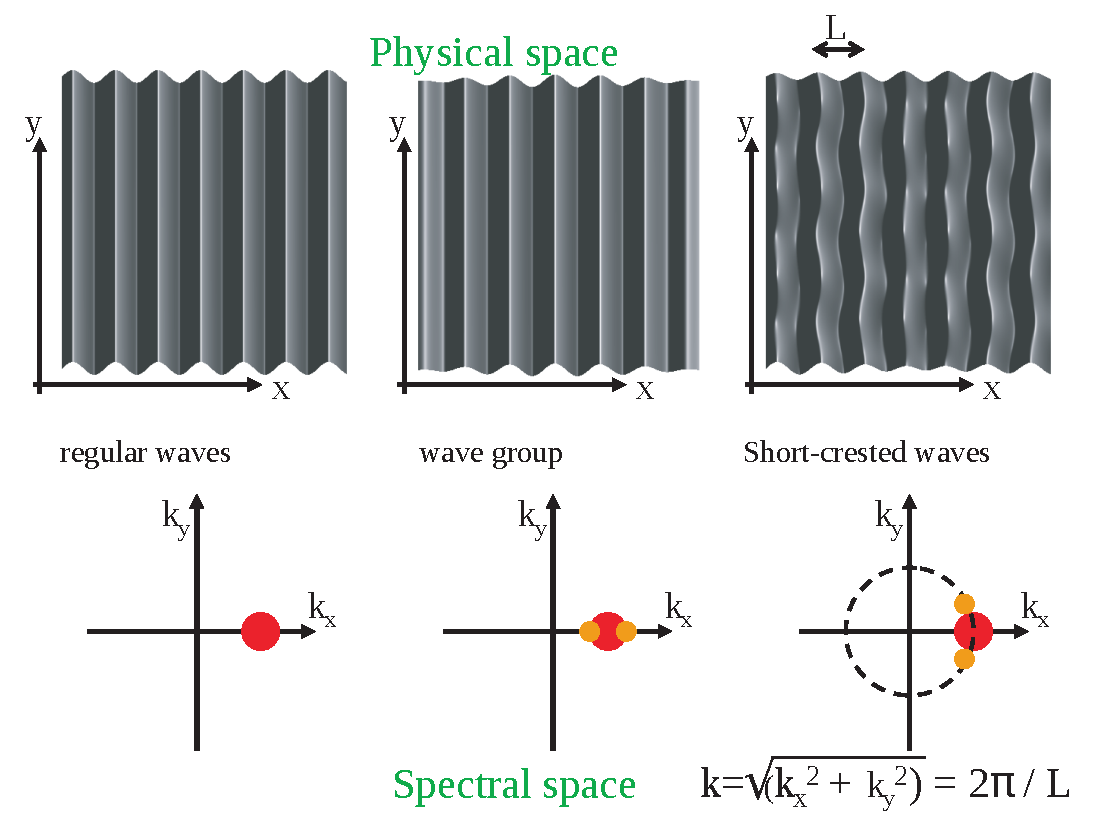
\includegraphics[width=0.8\textwidth]{FIGS_CH_MEASUREMENTS/spectres101_en.pdf}}
\caption{Relation between spectral and physical spaces. Schematic spectra of monochromatic waves (left panel) and modulated in terms 
of wavenumber or direction. For the last two cases, the surface is composed of three components.\label{fig:spectres101}}
\end{figure}
%%%%%%%%%%%%%%%%%%%%%%%%%%%%%%%%%%%%%%%%%%%%%%%%%%%%%%%%%%%%%%%%%%%%%%%%%%%%%
The reader is invited to try to recomposed a sea surface in the physical space from the spectrum produced by a numerical model,
\begin{equation}
\zeta(x,y,t)=\sum_{m}^{M}\sum_{n}^{N}\sqrt{2E(f_m,\theta_n)\Delta_f \Delta_\theta} \cos\left[ k_m \cos \theta_n x +k_m \sin \theta_n  y- \sigma_m + \Theta_0(m,n)\right],
\label{eq3.11}
\end{equation}
where $\Delta_f$ and $\Delta_\theta$ are the spectral resolutions, and $M$ and $N$ are the number of frequencies and directions used to discretize the spectrum.  
Rigorously, $M$ and $N$ should be taken infinite, but we may start with the typical resolution of  a 
spectral wave model, of the order of 30 frequencies and 24 directions, with a significant level of energy in maybe only 20 components. If you want to get a more realistic surface it is best to interpolate the spectrum on a fine spectral grid, before taking the inverse Fourier transform. 

The component amplitude $\sqrt{2E(f_m,\theta_n)\Delta_f \Delta_\theta}$  is consistent with the fact that the total variance 
elevation is the sum of the amplitudes squared divided by two, or the spectrum integral over the entire spectral domain. 
The phase $\Theta_0(m,n)$ can be taken randomly distributed over [0,2$\pi$]. The resulting surface will look smoother than 
an actual sea state, and the observed crest-trough asymmetry will not be reproduced. This is due to the random phase assumption 
that disregards the phases coupling between spectral components. You may add some nonlinear effects with the "choppy" method, shifting your elevation map using an estimate of horizontal displacement, giving more realistic wave crest shapes \citep{Nouguier&al.2009}.  %These issues are further addressed in \S\ref{random_harmonics}.

\section{Using spectra}
Skipping here the technical details necessary for a practical estimation of the spectrum  (see chapter \ref{ch_anaspec}), we now have a spectrum. Very nice, but what 
can we do with it? 

\subsection{Transfer function}\label{sub:transfer}
Depending on the application, one can transform the elevation variance spectrum. For a variable $A$ (for instance the bottom pressure), related to the  
surface elevation through a linear relation:
\begin{equation}
A=M\zeta,
\label{eq3.12}
\end{equation}
where $M$ is a complex number that takes values in the spectral space, the variance spectral density of $A$, $E_A$ is 
\begin{equation}
E_{A}(k_{x},k_{y})=|M|^{2}E(k_{x},k_{y})~\mathrm{or}~ E_{A}(f,\theta)=|M|^{2}E(f,\theta)
\label{eq:transfert}
\end{equation}
or any other equivalent expression in other spectral coordinates. For instance, the bottom velocity variance will be given from the polarization relation (\ref{polzeta})--(\ref{xi3}), that yield 
$M=\sigma \cos(\theta)/\sinh(kD)$, with $\theta$ the angle between the $x$-axis and the wave direction of propagation. We hence 
get the spectrum of the $x$-component of the bottom velocity.

Two of the most commonly used transfer functions are $M=\sigma$ for getting the surface orbital velocity magnitude in deep water, hence $M^2=4\pi^2 f^2$, and $M^2=\rho_w g/C_g=\rho_w g/(4 \pi f)$ for getting the energy flux in deep water. Using these transfer functions you get the surface orbital velocity variance 
\begin{equation}
<u^2+v^2>_{z=\overline{\zeta}}   =4\pi^2  \int_{0}^{\infty}  f^{2} E(f) {\mathrm d}f = 4\pi^2 m_2
\label{eq:moment_def}
\end{equation}
where $m_2$ is the second moment of the spectrum, and in general the  \textit{p-th} moment of the spectrum is defined as,
\begin{equation}
m_{p} = \int_{0}^{\infty}\int_{0}^{2\pi} f^{p} E(f,\theta)d\theta df
\label{eq:moment_def}
\end{equation}
Now, you may wonder why somebody would like to know the variance of the orbital velocity, well, it comes up, for example in Morison's equation that is the most widely used equation in offshore engineering to estimate forces on a structure \citep{Boccotti2000}, and other variances will matter for other applications. 

\subsection{Spectral and integral parameters: $H_s$, $T_p$ ...}\label{sub:param}
It can
be inconvenient  to describe a sea state by a two-variable function. Even when it is discretized into a numerical model,  typically 
over 30 frequencies and 24 directions meaning 720 spectral components, which is a lot of numbers to describe a sea state. This information can be 
summarized into a few meaningful parameters.

As the spectrum is a decomposition of sea surface variance, the most important parameter is certainly the variance $E$, often abusively called
energy. From the elevation variance $E$, we get a length scale  $\sqrt{E}$. Going back to sine waves, the variance is $a^2/2$ with $a$ the wave amplitude. Hence $\sqrt{2 E}$
is an equivalent amplitude  for random waves. More precisely, it is 
the root mean square amplitude. The root mean square wave height for a random wave is thus twice this amplitude
$H_{\mathrm{rms}}=2 \sqrt{2E}$.

For practical applications, the most widely used height scale is the \textit{significant wave height} $H_s$ that corresponds to the visual 
feeling given by the sea. From the wave height distribution we can define $H_{1/3}$ (see chapter \ref{ch1}). From the spectrum we define,
\begin{equation}
H_s \equiv H_{m0}\equiv 4 \sqrt{E} = 4 \sqrt{\int_{0}^{\infty} E(f) {\mathrm d}f}
\label{eq3.14}
\end{equation}
In practice $H_{m0} \simeq H_{1/3}$, this property can be demonstrated in the limit of a narrow spectrum \citep{Longuet-Higgins1952}. Following the recommendations of 
the World Meteorological Organization, 
we shall consider $H_{m0}$ to be \emph{the} definition of the significant wave height $H_s$. The "$m0$" index indicates that it is based on the zeroth moment of the spectrum. 


In many cases, the directional information is not available, and we only have the frequency spectrum $E(f)$. 
This distribution of the energy as a function of frequency contains information on the typical time scales of the signal. $E(f)$ generally exhibits 
a sharp maximum around the frequency $f_p$, $E(f_{p})=E_{\max}$. $f_p$ is the peak frequency, corresponding to the peak period $T_{p}=1/f_p$.  
This peak period can be noisy in the presence of several peaks, as in Fig. \ref{fig:Hawaii_spectrum}.
The frequency distribution can also be characterized from the spectral moments, $m_p$, 
\begin{equation}
T_{m0,p} =  \left[m_p/m_0\right]^{-1/p} \simeq \left[\left(\int_{0}^{f_{\max}} f^{p} E(f) df\right)/\left({\int_{0}^{f_{\max}} E(f) {\mathrm d}f}\right)\right]^{-1/p}.
\label{eq3.17}
\end{equation}
The most widely used periods are $T_{m0,-1}$, $T_{m0,1}$, $T_{m0,2}$. Each of these has a more or less weight on low frequency part of the spectrum.
If one is interested in an effect proportional to $f^2$, as is  the case of the wave forces exerted on a structure, it is reasonable to use $T_{m0,2}$.
Besides, $T_{m0,2}$ is very close to the mean period $T_z$ given by  wave-by-wave analysis. Note however that in practical calculations, $T_{m0,2}$ depends on the choice
of $f_{\max}$. The values of the different periods for a typical spectrum are shown in figure 
\ref{fig:Hawaii_spectrum}.
%%%%%%%%%%%%%%%%%%%%%%%%%%%%%%%%%%%%%%%%%%%%%%%%%%%%%%%%%%%%%%%%%%%%%%%%%%%%%%%%%%%%%
\begin{figure}[htb]
\centerline{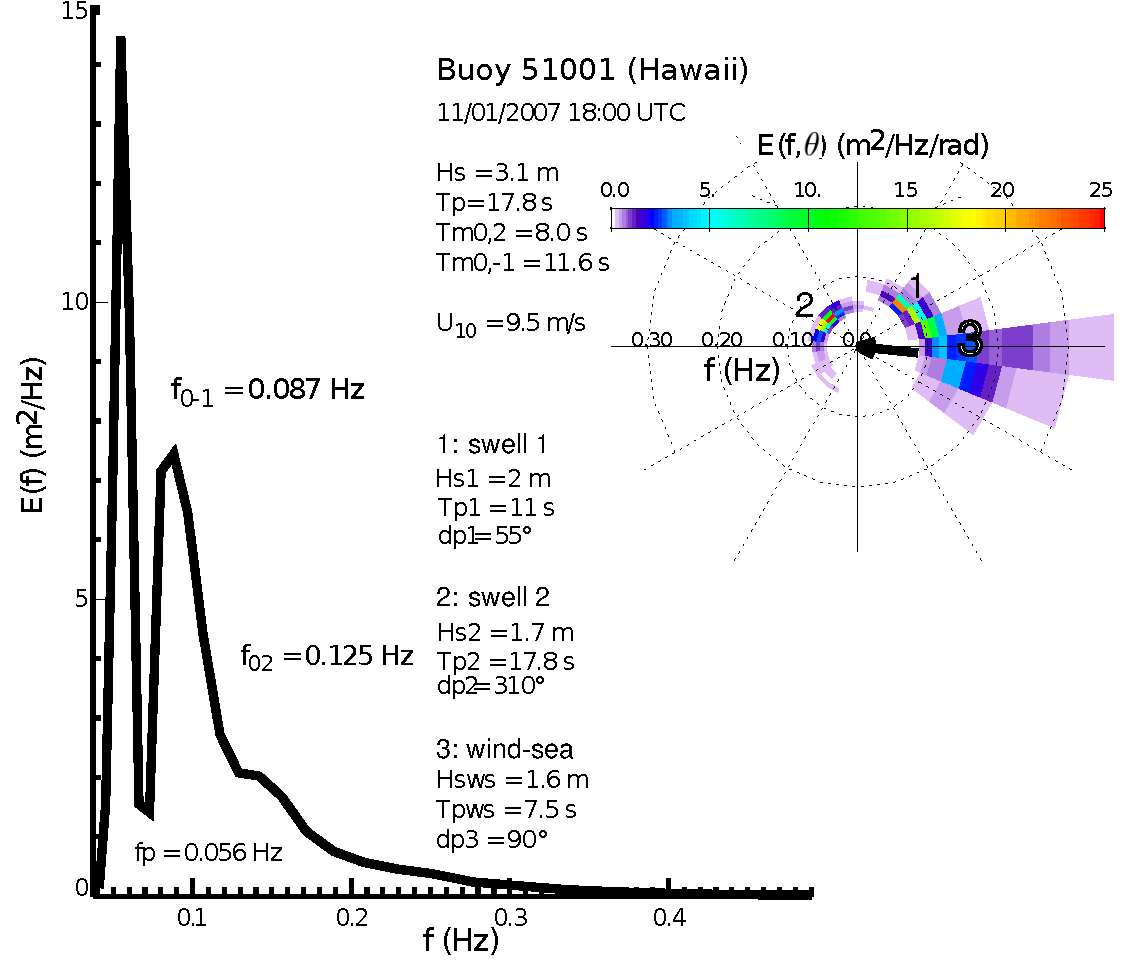
\includegraphics[width=0.7\textwidth]{FIGS_CH_MEASUREMENTS/exemple_spectre_Hawaii.pdf}}
\caption{
Typical example of a oceanic spectra in tropical area, measured by buoy 51001, moored 350 km North West of Kauai island, on January 11, 2007. 
The different peak and mean periods are indicated along with the parameters produced by a decomposition of the spectrum into a primary
swell, secondary swell and wind sea. This analysis is generally not possible without directional information. Note that the wind sea only appears 
as a soft "shoulder" to the right of the secondary swell, while it comes from a different direction. This shows the possible difficulty of 
separating swell and wind sea from a frequency spectrum. Also note that the significant 
wave height $H_s$ is less than the sum of $H_{s1}$, $H_{s2}$, $H_{sws}$, of the three systems: the energy can be summed but the wave heights cannot.
Namely $H_s=\sqrt{H_{s1}^2+H_{s2}^2+H_{sws}^2}$.}
\label{fig:Hawaii_spectrum}
\end{figure}
%%%%%%%%%%%%%%%%%%%%%%%%%%%%%%%%%%%%%%%%%%%%%%%%%%%%%%%%%%%%%%%%%%%%%%%%%%%%%%%%%%%%%%%%%%%


Finally, we define, 
\begin{eqnarray}
a_{1}(f) & = &\int_{0}^{2\pi} \cos{\theta} E(f,\theta)d\theta /\int_{0}^{2\pi} E(f,\theta)d\theta, \label{a1def} \\
b_{1}(f) & = & \int_{0}^{2\pi} \sin{\theta} E(f,\theta)d\theta /\int_{0}^{2\pi} E(f,\theta)d\theta ,\label{b1def} \\
\end{eqnarray}
that can be estimated from the elevation spectrum $E(f)$ and the elevation-horizontal displacements
co-spectra, $E_{xz}$ and  $E_{yz}$, as detailed in chapter \ref{ch_anaspec},   eqs. (\ref{Exz})--(\ref{Eyz}). 

The mean wave direction at frequency $f$ is, 
\begin{equation}
\theta_{m}(f)=\arctan(a_{1}(f)/b_{1}(f)),
\label{eq3.20}
\end{equation}
and the directional spreading, as defined by \cite{Kuik&al.1988} is the standard deviation (in radians) of the spectral width
in the limit of a narrow spectrum,
\begin{equation}
\sigma_{\theta}(f)=\left[2(1-(a_{1}^{2}(f)+b_{1}^{2}(f))^{1/2}) \right]^{1/2}.
\label{eq3.21}
\end{equation}
For equal energies in opposite directions, $\sigma_{\theta}$ is maximum at 
$\sqrt{2}$ radians, which is $81\,^{\circ}$. 

The directional wave properties of the dominant waves, can also be characterized with the 
mean direction and directional spreading of the spectral peak: $\theta_{m}(f_{p})$ and $\sigma_{\theta}(f_{p})$. 
$\theta_{m}(f_{p})$ is often referred to as "main direction", while the mean direction would rather be an average
over the entire spectrum,
\begin{equation}
\theta_{M}(f)=\arctan \left(\int_{0}^{\infty} b_{1}(f) E(f)df/\int_{0}^{\infty} a_{1}(f) E(f)df\right)
\label{eq3.22}
\end{equation}
With all these directions, one must be careful with the directional convention. The directions are usually counted
from North (direction 0), progressing clockwise (90 east, 180 south, 270 West). However, depending on the authors, the direction convention is either meteorological (direction
from where the waves or wind are coming, this is the convention used in the present manuscript) or oceanographic convention
(direction toward which the waves or currents are moving). Be careful!

 

 \section{Random waves \textit{in situ} observations}
 The most common usage of wave time series is the determination of the frequency spectrum $E(f)$ and, when more than 
 one variable are measured, the directional wave spectrum $E(f,\theta)$ may be estimated. Details of this processing 
 given in chapter \ref{ch_anaspec}. In practice, the most common in situ 
 instruments for wave measurements are surface-following buoys or bottom-mounted pressure gauges or ADCPs.  
 
 \subsection{Wave gauges}
 These are reference sensors that directly measures the free surface elevation $\zeta(x,y,t)$ at a fixed horizontal position $(x,y)$. 
 The measure is done through the 
electrical resistance or capacity of one (or two) conducting wires forming a loop closed by the sea surface. This type of sensor is widely 
used in the laboratory, but it is not so common at sea because this requires a fixed  platform
 and the wires are susceptible to damage by small floating debris. Also, the large wave heights encountered in the field require long 
 enough gauges. These wave 
gauges can also be mounted on a buoy that filters out the long waves through its motion \citep{Graber&al.2000}. Wave gauges are most often 
associated in an array (see below) of several gauges synchronized and mounted on a single platform so as to 
provide a wave direction estimation \citep{Cavaleri&al.1981}.

The direct measurement of surface elevation can also be performed by radar and LIDAR systems, which determine the  
distance to the sea surface from the travel time of an electromagnetic or sound wave, and that can likewise be arranged in an fixed array or integrated 
in a scanning system.


  \subsection{Wave buoys}
    Buoys measure either the successive positions and velocities, determined by a global navigation satellite system (such as the Global Positioning System - GPS) or 
    vertical acceleration recorded by a buoy floating at the free surface that give after a double integration in time, 
  a surface elevation signal $\zeta(x,y,t)$. Depending on the type of instrument and on the presence of currents, the horizontal position $(x,y)$ is not fixed but 
  nearly follows the wave orbital 
motion. This later property may be annoying for purists of the wave profile, as it partly filters out the free surface nonlinearity (the linear 
Lagrangian motion involves a part of the nonlinear Eulerian motion). In addition to the heave measurement, that was for long the most common, the wave 
direction can be determined by measuring the horizontal accelerations that yields, through double integration, the horizontal displacement $x$ 
and $y$ (figure \ref{Datawell_xyz}). 
\begin{figure}
\centerline{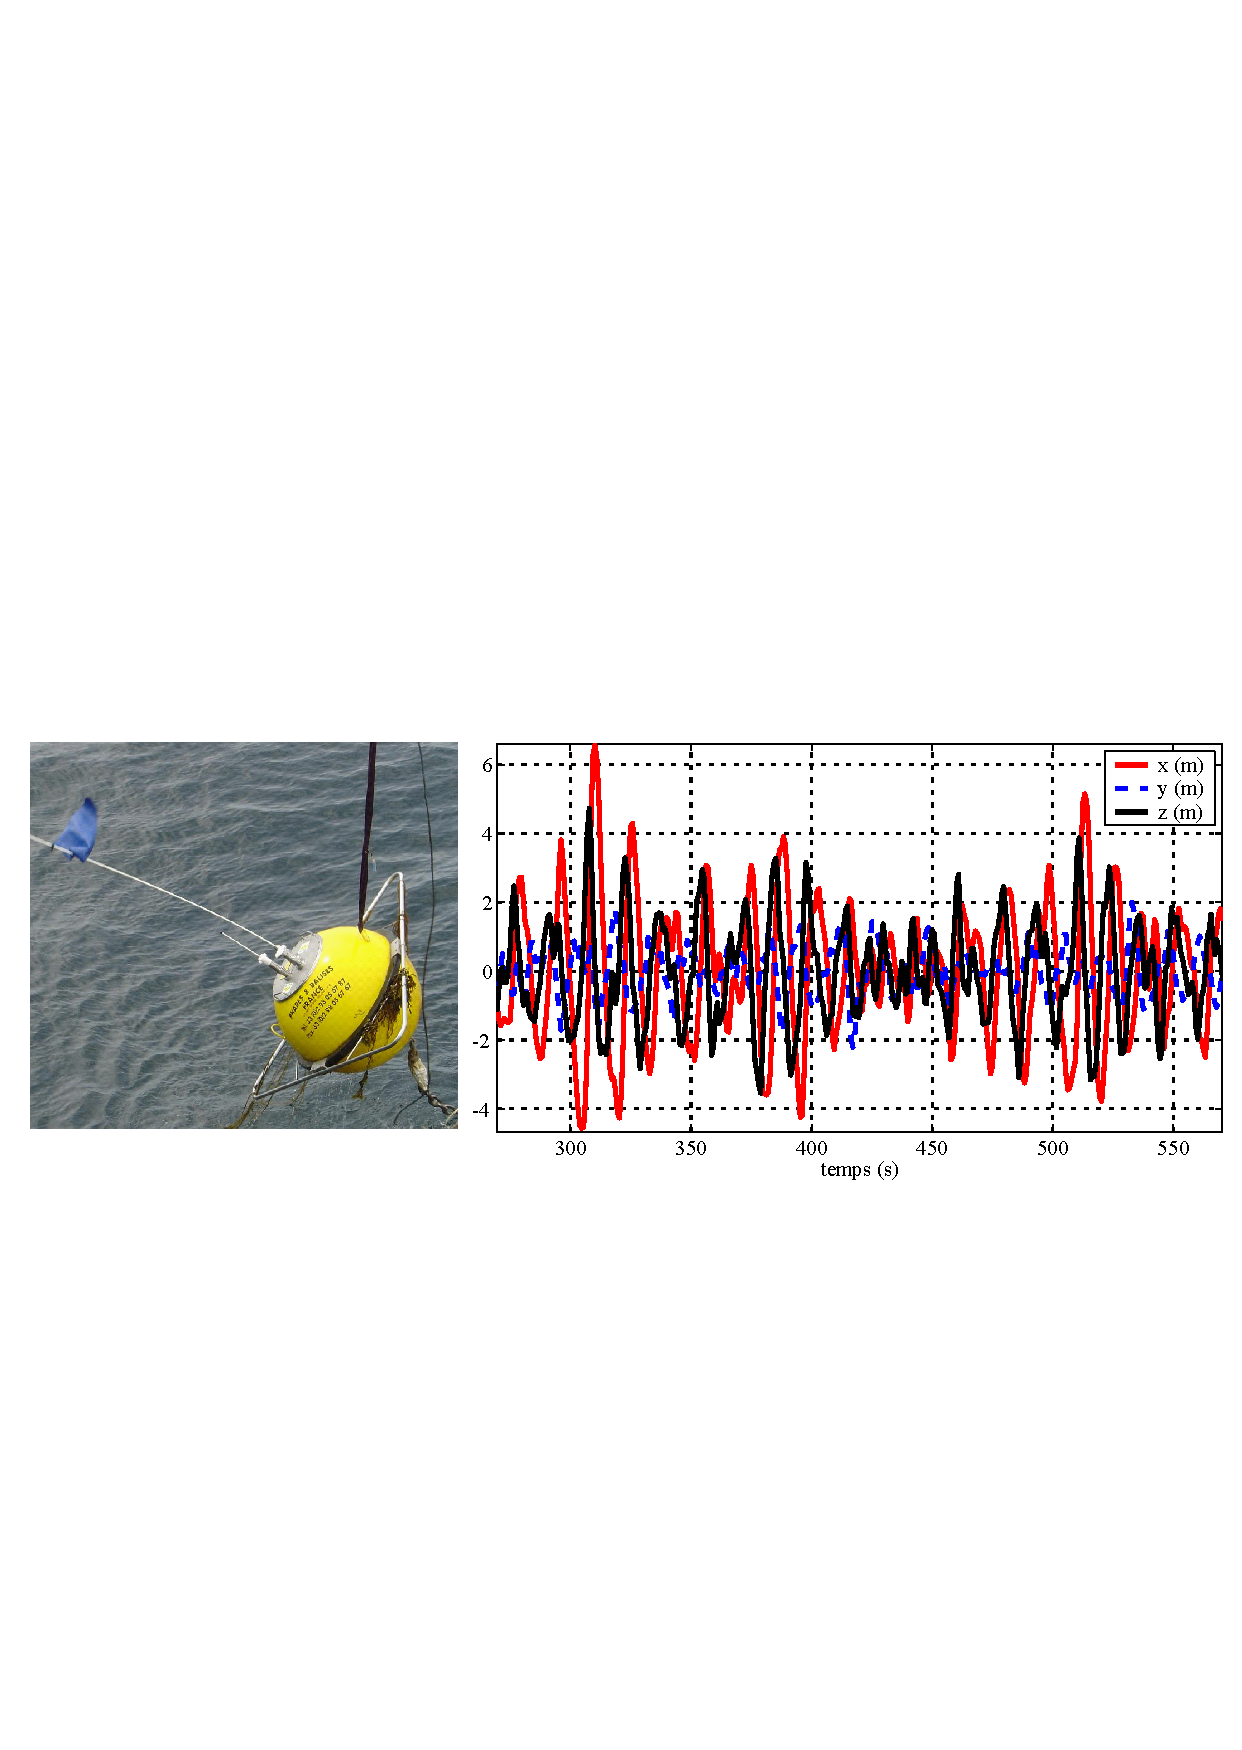
\includegraphics[width=\textwidth]{FIGS_CH_MEASUREMENTS/Exemple_DWIROISE2004all_plus.pdf}}
\label{Datawell_xyz}
\caption{Left panel: Deployment of a  Datawel Waverider buoy, 0.9 m of diameter, equipped with a (long) HF radio antenna and 
with a (short) Orbcomm satellite antenna for data transfer. Right panel: examples of displacements measured by this buoy offshore Crozon in May 2004. 
(same time series as in figure \ref{FigWaveriderTSz}). Of course, the 10~m high waves were not measured by the times of the buoy deployment.}
\end{figure}
 The use of  precise satellite positioning now allows a direct measure of the 3-component position and velocity, the latter being generally more accurate \citep{Herbers&al.2012}. Many companies have commercialized such buoys.

The largest buoys generally use a measurement of the components $\partial \zeta /\partial x$ and $\partial \zeta/ \partial y$ and of the local free 
surface slope: pitch and roll as the first prototypes of \cite{Longuet-Higgins&al.1963} and \cite{Cartwright&Smith1964}. This is the case of the US 
National Data Buoy Center (NDBC) 3-m diameter buoys.
Details of buoy processing are given in chapter \ref{ch_anaspec}. Both methods, acceleration and pitch-roll allow, thanks to the three signal covariance, 
the determination of the first four Fourier coefficients 
of the angular distribution, also known as angular moments,
\begin{itemize}
  \item  $a_1$ and $b_1$, defined by (\ref{a1def})--(\ref{b1def}) and calculated from the co-spectra $E_{xz}$ and $E_{yz}$ (equations \ref{Exz}--\ref{Eyz})
\item $a_2$ and $b_2$, defined as $a_1$ andf $b_1$ but with $\cos \theta$ and $\sin \theta$ replaced by $\cos 2 \theta$ and $\sin 2 \theta$, respectively.
\end{itemize}

A more complete measure of the directional spectra from floating buoys has been developed but has not been as successful as expected: the cloverleaf buoy that consists in three 
pitch-roll buoy linked to each other \citep{Mitsuyasu&al.1975}. In principle this layout provides a measure of the surface curvature and the Fourier coefficient up to $a_8$ and $b_8$.
From a conventional buoy, one has to infer the function $S(f,\theta)$ from only the four independent number $a_1$, $b_1$, $a_2$ and $b_2$. This is not so much a 
measurement problem, but rather one of choosing a statistical estimator. There are many method for this. Among these, the Maximum Entropy Method \citep[MEM][]{Lygre&Krogstad1986}, 
has the advantage of conserving the angular moment  $a_1$, $b_1$, $a_2$ and $b_2$. The MEM method tends however to 
to give a bimodal shape (two-peak spectra), which is often \citep{Ewans1998} but not always realistic \citep{Benoit&al.1997}.

Other recent analysis techniques aim at increasing the the directional resolution of this kind of measurements. For instance, \cite{Donelan&al.1996}, 
have proposed an interesting method based on a wavelet transform. Unfortunately their method assumes that for any given frequency 
the wave field is dominated by waves coming for one single direction, which is not the case. This analysis yields a very high directional resolution, and can be interesting 
to detect the presence of waves from a given direction, but it cannot be interpreted as a directional spectrum as it leads to a low bias in the directional spreading. Other methods can be biased and 
should be avoided. This is 
the case of the maximum likelihood method (MLM) which yields output spectra that are systematically too broad and have moments $a_1$, $b_1$, $a_2$ and $b_2$ that 
are different from the input parameters.
 
 \subsection{Pressure gauges}
 When surface elevation measurements are too expensive or not possible, which may be due to strong currents incompatible with mooring lines, breaking waves in the surf zone, a usually good alternative is the measurement from bottom-mounted sensors. The most common and robust are pressure gauges that can be used to measure 
 tidal elevations at the same time. To recover the surface elevation from the pressure signal, we can invert the linear transfer function given by eq. (\ref{pression}), 
 namely, for a sensor at a height $h_d$ over the bottom,  $M=\rho_w g \cosh(kh_d)/\cosh(kD)$, with $k$ estimate from the frequency $f$ of each spectral component of the time series, using the Airy wave dispersion relation. In shallow water and for waves of large amplitudes, this method often underestimates the wave height because the linear dispersion is not very accurate \citep{Filipot&al.2010,Bonneton&Lannes2017}. The water depth $D$ is also given by the measurement of 
 the mean pressure once it is corrected for the atmospheric pressure. Because the elevation to pressure transfer function $M$ decreases when  $k$ increases, it is usually impossible to recover  wave elevations for frequencies above a cut-off value $f_c$. That value $f_c$ is a function of water
 depth, instrument noise, background noise (usually due to currents), but also of the directional wave spectrum. Indeed, figure \ref{fig:pressure_with_2ndorder}
 shows an example of data recorded in 100~m depth, in which the second order pressure is larger than the linear pressure for frequencies above 0.13~Hz. As discussed in part 3, 
 this second order spectrum is a function of the frequency spectrum $E(f)$ but also of the directional wave distribution. In that case, it is not possible 
 to recover $E(f)$ for frequencies above 0.12~Hz. For example, on day 4, the yellow-orange sloping line at frequencies 0.05 to 0.1 Hz is 
 a due to swell waves arriving from a distance of about 4000~km (see explanations in chapter \ref{ch3}, eq. (\ref{prev lin1})). 
 At the same time, there is a fainter blueish line at twice these frequencies which is caused by the 
 second order effect. The vertical blue stripes above 0.13~Hz are caused by the tidal current effects on the directional wave spectrum \citep{Ardhuin&al.2013}.
 %%%%%%%%%%%%% figure
\begin{figure}[htb]
\centerline{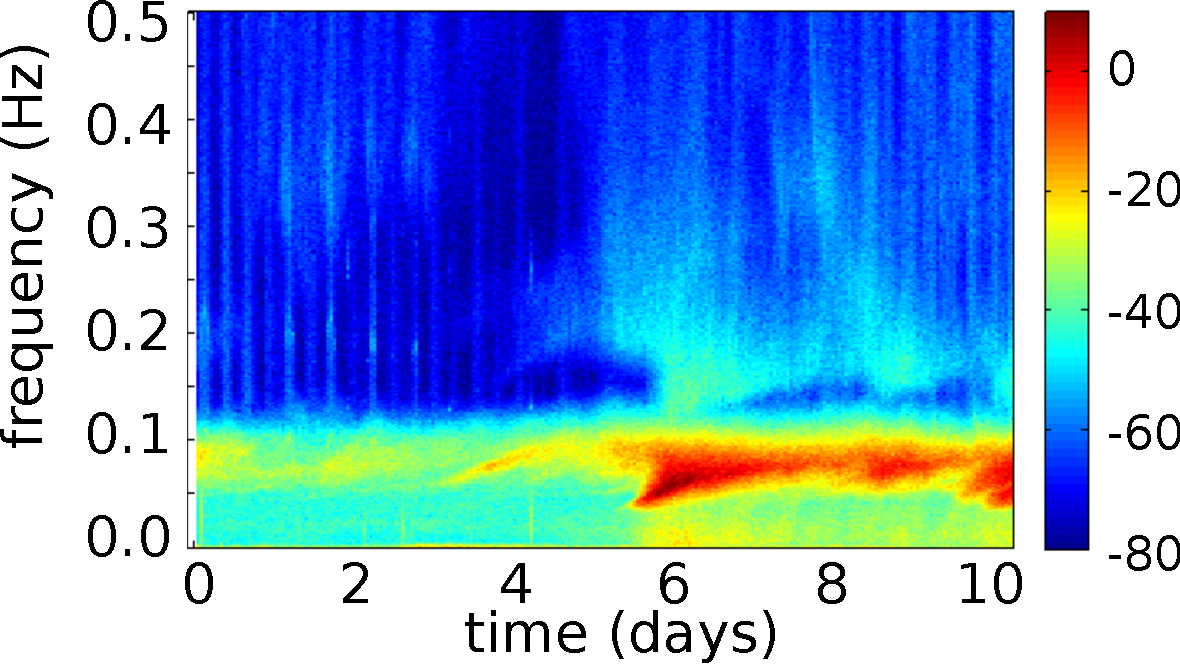
\includegraphics[width=0.7\textwidth]{FIGS_CH_MEASUREMENTS/pressure_with_2ndorder.pdf}}
%\vspace{3.64in}
  \caption{Bottom pressure spectra}
    {Time-frequency diagram of the pressure recorded over 11 days in 100~m depth off the French Atlantic coast in October 2015.  The colors show the pressure level in dB relative 
    to 1~m$^2$/Hz times $\rho_w^2 g^2$. These measurements were performed by a very sensitive Paroscientific piezo-electric sensor, included in a RBR-duo 
    system, with a noise level below -80 dB. At our depth of 100~m, the usual linear pressure signal, with a level between -40 to 10 dB, can be used to recover 
    the surface elevation spectrum for frequencies below 0.12~Hz. At higher frequencies, the pressure is dominated by a second order effect due 
    to waves in opposite directions \citep[e.g.][]{Miche1944b,Ardhuin&al.2013}. That effect has very important consequences for seismology, as discussed in part 3.} \label{fig:pressure_with_2ndorder}
\end{figure}
%%%%%%%%%%%%% end of figure

 
\subsection{P-U-V sensors}
As indicated by its name, this sensor measures the pressure $p$ and the two horizontal components of the velocity, $u$ and $v$. It is indeed the 
combination of two instruments: a current meter (acoustic, electromagnetic because a high sampling rate is required) and a pressure sensor, often 
piezo-electric. This instrument is of particular interest as it is designed to be installed on the sea bottom. It is the simplest mooring you may imagine, if one 
is not too worried about fishermen, for instance. Of course, it is difficult ut not impossible to recover real time data (cables, acoustical modems with surface buoys...).

We have seen in Chapter 2 that the fluid pressure and velocities exponentially decay from the surface to the bottom with a typical scale which correspond 
to the wave length 2$\pi/k$. The "P-U-V" sensor is thus perfect if one wish to measure the agitation at the bottom. To measure the wave heights one may use
the theory that provide transfer functions between pressure, velocities, elevation, etc (equation \ref{eq:transfert}). In this situation, the closer to 
the surface, the more reliable will be the measurement (e.g. an instrument mounted on a floating of fixed platform).

 \subsection{Sensor arrays and ADCPs}
A set of wave gauge can be combined to record more covariances between the measurements. This kind of 
measure allowed to get the first accurate spectra \citep{Donelan&al.1985} and is particularly used for the air-sea interaction studies, 
for which the short waves spectrum is crucial \citep{Graber&al.2000, Pettersson&al.2003}. It is essential to synchronize the sensors with 
an accuracy that is small compared to the measured wave period. Similar techniques are employed in RADAR and SONAR technologies to determine the sources of echoes. The original array processing algorithms 
used for waves were actually developed for seismology.

 These techniques have been largely applied to pressure sensors arrays with a number of statistical methods for the spectrum estimation 
 \citep[e.g.][]{Davis&Regier1977, Long&Hasselmann1979, Pawka1983, Herbers&Guza1990}. An example of a spectrum is given in Figure \ref{wave spectra} 
determined from a coherent array of pressure sensors deployed in 8m depth on the site of the US Army Corps Field Research at Duck, North Carolina. 
For large arrays, the underwater instruments positioning much be very accurate. An acoustical positioning is generally used.
%%%%%%%%%%%%% figure
\begin{figure}
\centerline{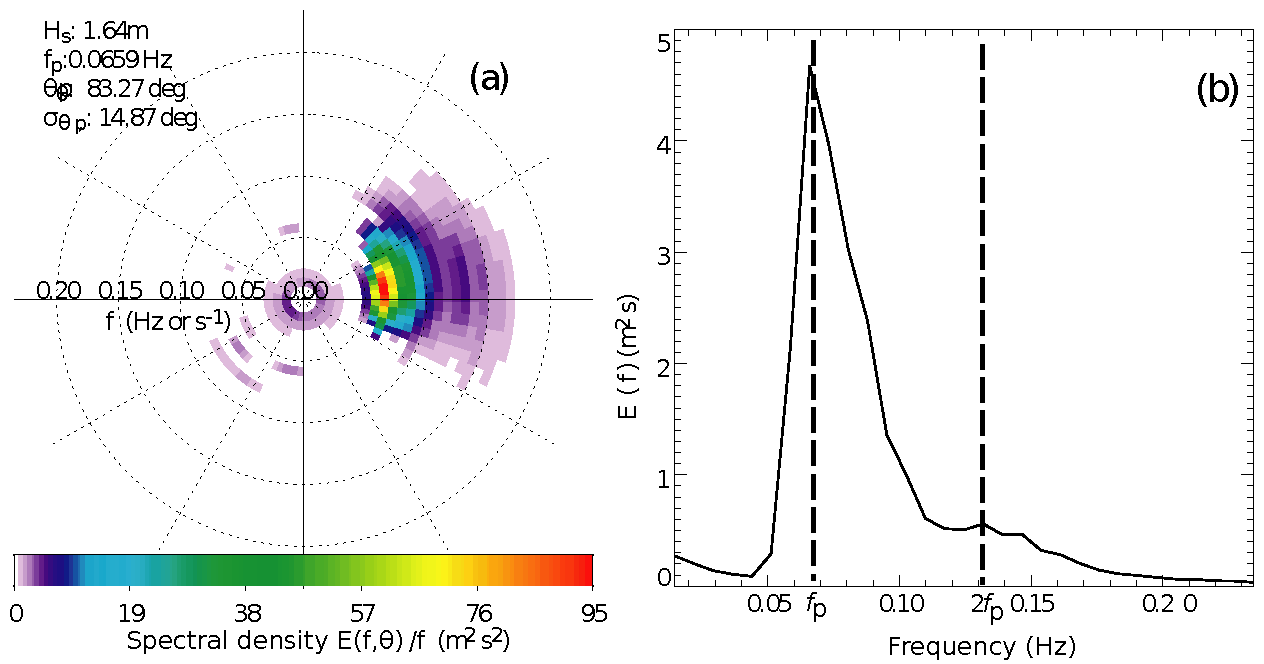
\includegraphics[width=0.6758\textwidth]{FIGS_CH_MEASUREMENTS/introduction_fig1.pdf}}
\caption{(a) Example of frequency-direction wave spectra, divided by frequency, computed from 8m depth pressure measurements in Duck, NC, October 
19, 1994, 7:00 (EST). (b) Corresponding Frequency spectra whose secondary peak matches the first harmonic of the spectral peak 
($f=2f_p$), and which is likely due to the effect of nonlinear interactions that are of great importance in shallow water.}
\label{wave spectra}
\end{figure}
%%%%%%%%%%%%% end of figure
  The directional resolving power of the array generally increases with the number of sensors in the array \citep[see][]{Kinsman1965}. 
  Arrays of pressure sensors are excellent reference instruments for measuring the spectra of dominant waves,  but they 
are relatively expensive to deploy and maintain. \cite{OReilly&al.1996} used such an array for the validation of directional properties of two different types of 
buoys. %However, comparisons have shown that for the parameters estimated from the the moments  $a_1$, $b_1$, $a_2$ and $b_2$, 
%the Datawell wave buoy, for instance, gives excellent results \citep{OReilly&al.1996}. Sensors arrays get useful only when further details on the 
%wave spectra are required (separation of incident and reflected waves, or of different wave systems, etc...). 

A recent and convenient alternative is the use of current profilers (ADCP).  The combination of the velocities measured by different acoustic beams, 
allows, in principle, for an interesting measure of the directional spectra. However, the typical noise of up-looking ADCPs does not allow a 
higher angular resolution than that of a simple P-U-V \citep{Herbers&Lentz2010}. The main benefit of ADCPs, however, is the use of measurements close to the sea surface, 
where the wave motion is less attenuated than at the bottom. 

\section{Optical measurements}
Waves are usually the first thing that you see when looking at the sea. But turning beautiful pictures into numbers for scientific analysis is 
not so easy. We will not discuss here the techniques that are mostly used in the laboratory (e.g. light refraction across the air-sea interface), but 
instead we present the main methods in use for application to real ocean waves. 
\subsection{From stereo-photography to stereo-video}
The first methods used to measure wave shapes were based on stereo-photography: pairs of photographs taken at the exact same time can be analyzed to 
produce a 3D map of the sea surface \citep{Schumacher1939}. The basic principle is to determine the $(x,y,z=\zeta(x,y))$ coordinates of points that have been 
identified in both images. This identification can be done using automatic correlation analysis. The pair of pictures can be obtained from a single platform to cover a modest area and reveal interesting 
details about the wave shapes \citep{Banner&al.1989}, typically less than 30 by 30~m, 
or from a pair of aircraft to get a view of a much broader region \citep{Cote&al.1960,Holthuijsen1983b} and produce a full directional 
wave spectrum. 
%%%%%%%%%%%%%%%%%%%%%%%%%%%%%%%%%%%%%%%%%%%%%%%%%%%%%%%%%%%%%%%%%%%%%
\begin{figure}[htb]
  \center{\noindent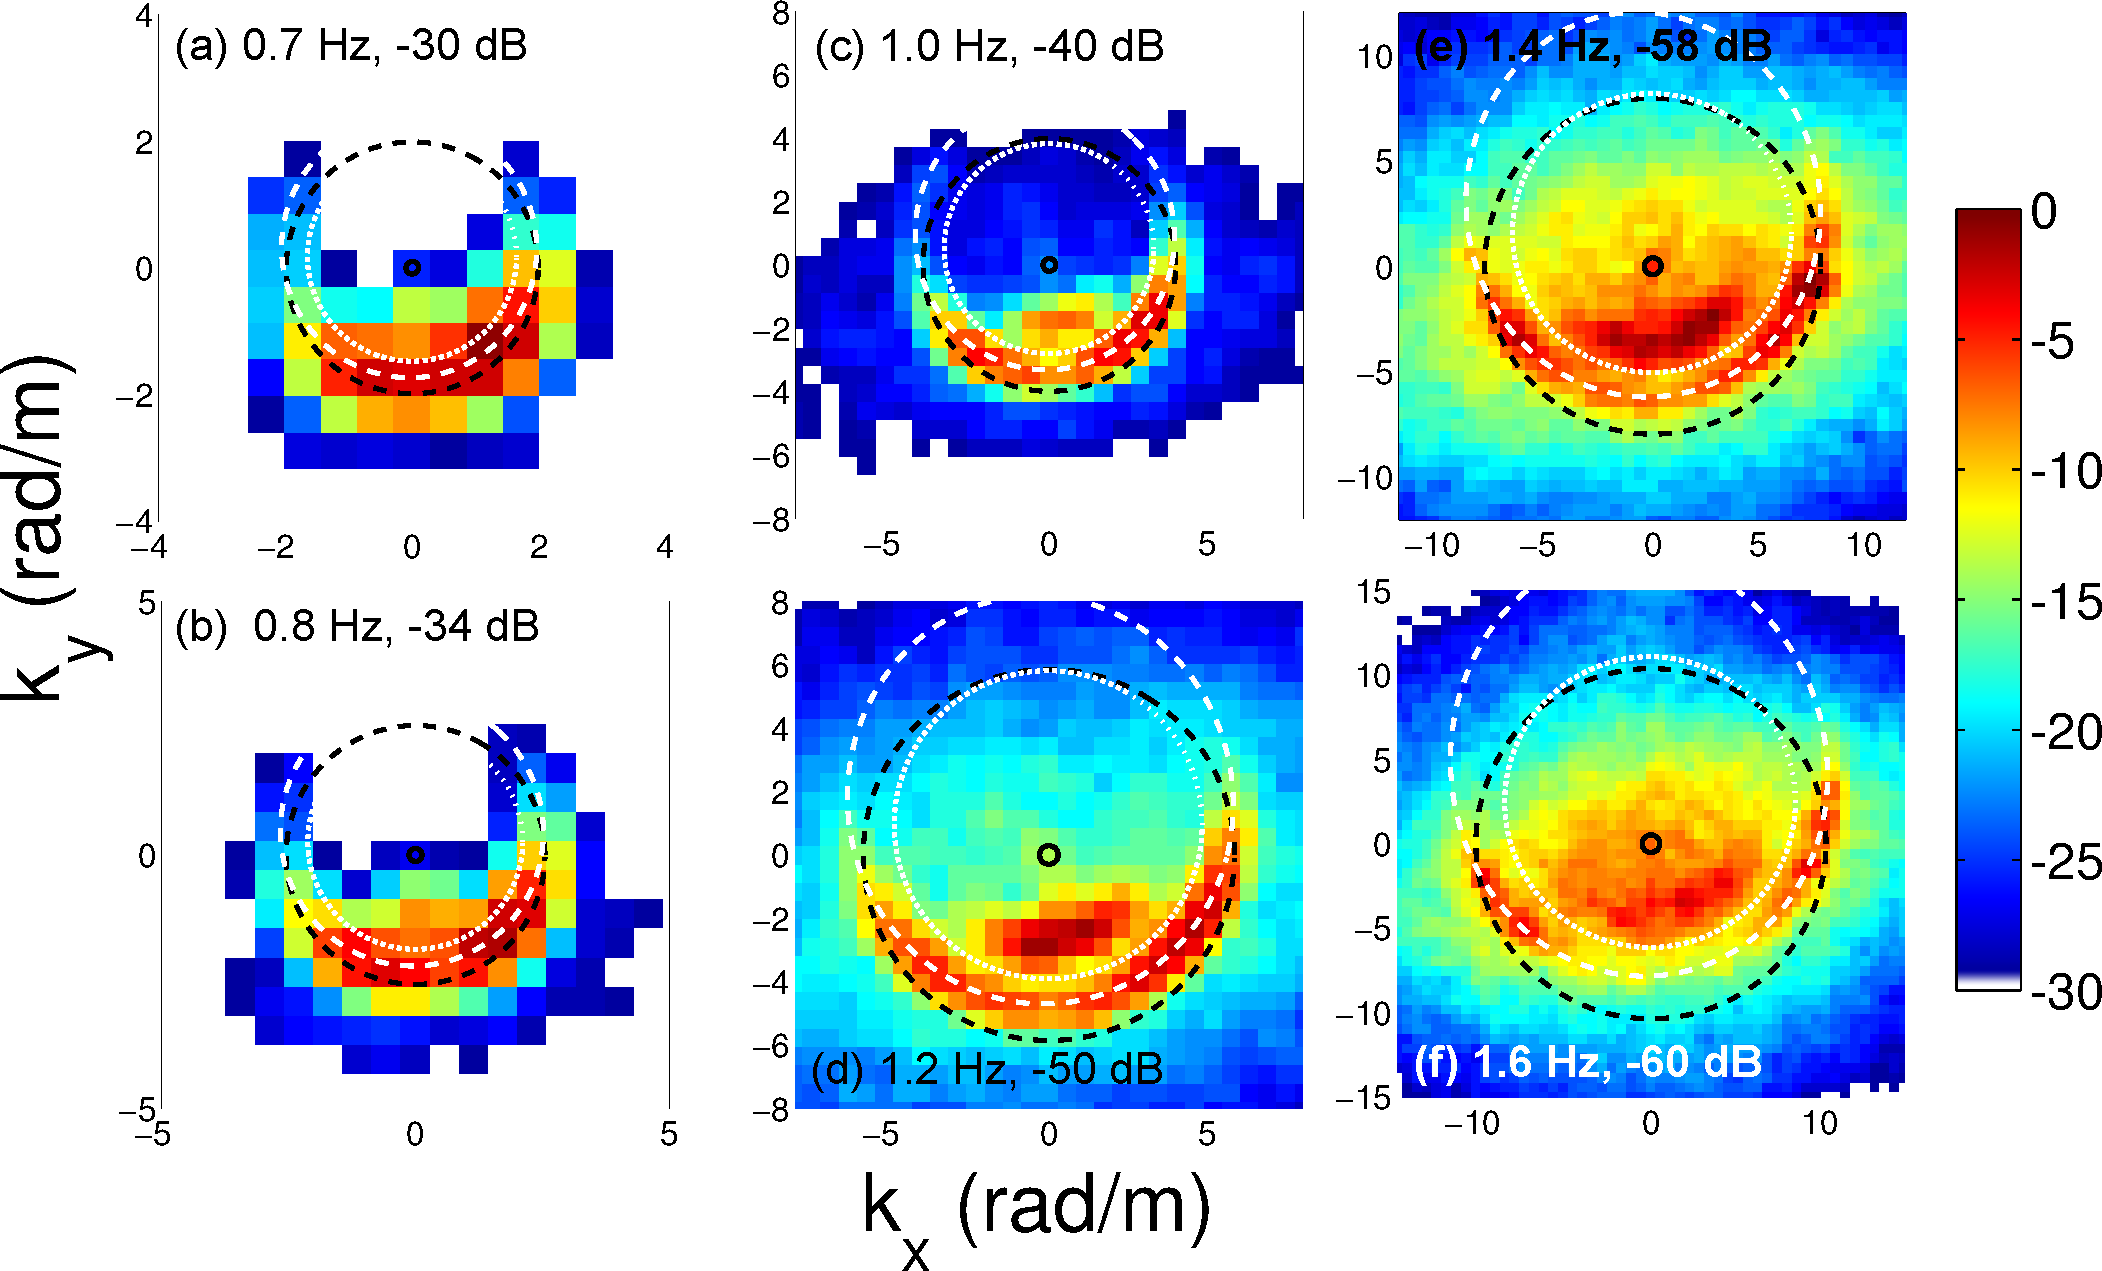
\includegraphics[width=0.8\linewidth,angle=0]{FIGS_CH_MEASUREMENTS/kxky_spec1_nosmooth.pdf}}\\
  \caption{Slices of the double-sided spectrum for positive apparent frequencies 0.7, 0.8, 1.0, 1.2, 1.4 and 1.6 Hz. The energy appears in the direction from 
           where it is coming. For each panel the color scale spans 30 dB with the dark red corresponding to the power indicated on 
the figure (e.g. -30 dB) relative to 1~m$^4$/Hz. Note that 1.4 and 1.6 Hz are twice 0.7 and 0.8 Hz, so that the first harmonic of the components in (a) and (b) 
           appear at approximately twice the wavenumbers in panels (e) and (f). In each panel, the linear dispersion relation without current is plotted in black, and the  white dashed line gives the linear dispersion with a uniform current $U= 0.15$ m/s oriented towards the trigonometric angle 99 degrees. The white dotted  line marks approximately the separation between 
the linear part of the spectrum and the faster non-linear components (Adapted from Leckler et al. 2015). } \label{fig:kxky}
\end{figure}
%%%%%%%%%%%%%%%%%%%%%%%%%%%%%%%%%%%%%%%%%%%%%%%%%%%%%%%%%%%%%%%%%%%%%
Now that everyone is carrying a digital camera around, and that stereo processing is much more common, there are many opportunities 
to measure the full evolution  of the sea surface in space and time $\zeta(x,y,t)$. Recent efforts by \cite{Benetazzo2006} and \cite{Gallego&al.2011} 
have demonstrated the capabilities of stereo processing, leading to new applications \citep{Fedele&al.2013,Leckler&al.2015}. Latest developments include  
auto-calibration and the proper motion corrections needed for ship deployments. A general issue that remains is that not all light conditions are favorable. Alternatively, the use of 
more expensive infrared cameras or polarization cameras is a very interesting extension for overcoming the variability of lighting conditions and 
the lack of texture at small scale 
for a correlation analysis \citep{Sutherland&Melville2013,Laxague&al.2015}.

The great advantage of having the full surface $\zeta(x,y,t)$, is that we can now measure a 3D spectrum, without the need to use linear wave theory. 
This is most important for the short wave components, for which nonlinear contributions are important. Figure \ref{fig:kxky} shows slices of the 3D spectrum 
at a constant frequency. These are obtained from a stereo-video system installed 11~m above the water in a platform in the Black Sea. The image processing 
uses the epipolar method: the position of the sea surface is obtained only by a knowledge of the geometry of the camera system.
This record from October 4, 2011, was acquired when the wind speed was 14~/s and the wave  peak frequency is $f_p=0.33$~Hz \citep{Leckler&al.2015}. The 
Non-linear contributions to the frequency spectrum dominate for $f > 4 f_p$. For example at $f=1.2$~Hz, there is more energy in the peak located near $(k_x=0,k_y=-3)$ 
than along the linear dispersion relation shown wit the white dashed line. 
Such non-linear effects are also important for the statistics of extreme wave heights, as shown by \cite{Fedele&al.2013} and \cite{Benetazzo&al.2017}.



\subsection{Using polarization and/or light intensity}
Such a stereo system has difficulties in measuring waves with frequencies higher than 1.4~Hz that have small heights. Other measurement techniques that 
are directly sensitive to slopes are better suited for these shorter components: these include polarimetry \citep{Zappa&al.2008} or a measurement of 
the radiance that can also be combined with the epipolar method \citep{Gallego&al.2011,Yurovskaya&al.2013}. 

Such a technique can also be applied to high resolution airborne or satellite imagery (with pixel sizes less than 30~m in order to resolve waves). 
\cite{Kudryavtsev&al.2017} have particularly taken advantage of the O(1~s) time lag in the acquisition of the different color channels of the Multi Spectral Instrument 
on board Sentinel-2. Clouds or haze obviously limit the application of optical methods, which is why radar is often preferred for wave remote sensing. 



\subsection{Surface wave radar}
An extreme case of grazing angle occurs when the radar waves propagate along the surface. This kind of propagation is possible
in the HF-VHF range (from 2 to 50 MHz). This surface wave allows indeed to get information beyond the horizon. 

%%%%%%%%%%%%% figure
\begin{figure}[htb]
\centerline{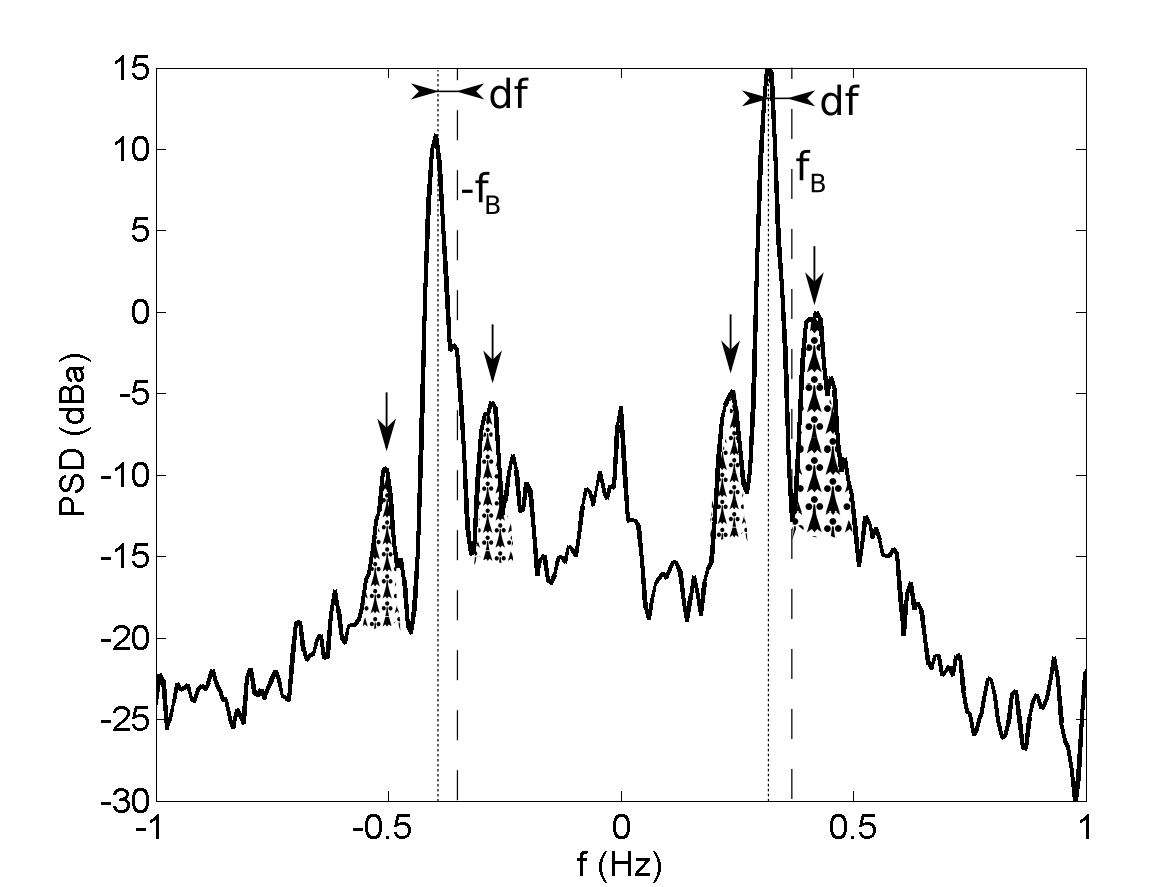
\includegraphics[width=0.5\textwidth]{FIGS_CH_MEASUREMENTS/Spectre_bin_10_touch.png}}
%\vspace{3.64in}
  \caption{Example of Doppler spectrum from a HF radar.}{This measured spectrum comes from the Porspoder radar (Finistere, France). 
The radar frequency is 12.4~MHz, corresponding to a wavelength $L_e=2 \pi/k_e=24$~m. The main echoes is due to Bragg scattering, 
which selects the ocean waves with a wavelength $L_e/2=12$~m that propagate towards ($f > 0$)  or away from the radar ($f<0$). 
Multiple scattering by waves with wavenumbers  $\kb_1$ and $\kb_2$, such that $2 \kb_e = \kb_1 + \kb_2$
gives the 'second order echoes'. At first order, i.e. for linear waves, the waves of wavenumber $k_w=2 k_e$ 
have a frequency $f_B=\pm \sqrt{g 2 k_e} =\pm 0.36$~Hz  in deep water. The anomaly $df$ of the two highest peaks in the Doppler spectrum 
indicate that the phase speed $2 \pi f / k$ is different from the linear wave theory without current. 
the main reason for that difference is usually the presence of a current, with a velocity $U_r=2 \pi df / (2 k_e)$ in the direction of the radar. }\label{HFspectrum}
\end{figure}
%%%%%%%%%%%%% end of figure

The radar reflection is well explained by Bragg theory, with the maximum backscatter power at the Doppler frequency $f_D$ occuring for 
electromagnetic incident and reflected wave numbers vectors $\kb_i$ and $\kb_r$ that match with the wavenumber $\kb_w = \pm \kb_i \mp \kb_r$ 
and and the wave frequency $f_D=f$, where $f$ and $\kb_w$ are related by the linear dispersion relation. 
In the monostatic configuration where the receiving and transmitting antenna are almost at the same place, we have $\kb_i = \kb_e$,  $\kb_r= - \kb_e$, 
and $\kb_w = 2 \kb_2$. 

The observed Doppler spectrum can be
interpreted as the superposition of simple reflections (or first order reflections) and multiple reflections. 
The extraction of sea state spectra is possible from the second order that is a convolution of the spectrum 
\citep[see for instance][]{Wyatt2000}. These second order echoes are weaker than first order echoes at Bragg frequencies. The main echoes are used for currents measurement. Their frequency provides a measurement of the Bragg wave phase velocity. The deviation 
of this phase velocity from the expected linear wave phase speed can be interpreted as a surface drift current \citep{Ardhuin&al.2009b}. 
This current includes non-linear corrections to the phase velocity, which is like a filtered Stokes drift \citep{Stewart&Joy1974,Broche&al.1983,Ardhuin&al.2009}.
The secondary peaks are caused by either the multiple reflection of radar waves, or the single reflection off nonlinear wave components. 
In some cases a peak can be seen at the frequency $\sqrt{2}f_B$ which corresponds to the reflection from the first harmonic of waves with wavenumber 
$\kb = \pm \kb_e$, which have a frequency, $2\sqrt{g k_e}$ in deep water. Because different wave components have different sensitivities to the current profile, 
it is possible to use that peak to measure the vertical shear of the current \citep{Ivonin&al.2004}. 


%\section{The limitations to the usual wave spectrum}
%The spectrum gives the full statistical properties of waves, provided the components are effectively independent. Yet, this is not exactly true as waves are slightly nonlinear. Two main relations exist between components: the presence of harmonics and modulations. The first effects comes from the fact that a single nonlinear wave train corresponds to several spectral components whose wave number and frequency are multiple of that of the carrier wave. Rigorously speaking, one needs the 3D spectrum $E(f, \mathbf{k})$ to discern these harmonic waves that do not follow the linear dispersion  (Figure \ref{fig:kxky}). The 3D spectrum estimation requires specific instruments, mapping the surface in space and time. The link between the  3D spectrum and the linear part of the spectrum is the topic of ongoing research. The calculation technique of dressed and undressed spectrum presented by  \cite{Elfouhaily&al.2003}  is a possible approach: the undressed spectrum corresponds to the linear part and the dressed part to the nonlinear spectral contents. To lowest order, however, the full spectrum  can be obtained by the second order correction \citep{Janssen2009,Leckler&al.2015}. 

%The modulation effect is a bit more complex. Typically, short waves in the presence of much longer waves see their environment modified. In particular, the apparent gravity felt by short waves is the standard gravity plus the vertical acceleration induced by the longer waves motion. In the same fashion, the long waves orbital velocities acts as a variable current on the short waves.  These effects are one of the likely causes of the higher breaking rate of short  waves at the crest of long waves \citep{Dulov&al.2002,Guimaraes2018}. The short wave spectra is hence modulated by the long waves. In practice, for the wind sea, such effects are weak for waves with frequency less that three times the peak frequency \citep{Banner&al.1989}. This factor 3 on the frequency corresponds to a factor 10 on the wavelength (in deep water).

%Modulations can be caused by other effects than the presence of other waves. In particular, if the medium in which the wave propagate is not homogeneous, then the wave field will contain wavelengths that are interferences between the medium and the waves, and that do not correspond to the linear dispersion relation.  These non-homogeneities can be variations in water depth, current, gravity, surface tension ... 

%If these modulations occur  at scales similar to the wavelength, besides the local effect on the waves there is also a scattering of the waves with the generation of waves in other directions, frequencies, or other types of waves, such as the Bragg scattering  caused by underwater topography that is described in chapter \ref{ch5}, or the generation of seismic waves over a sloping bottom in  chapter \ref{chsismo}. These scattering effects result in an evolution of the spectrum in space and time. 

%If the scales are shorter than the wavelength, then the medium is a 'meta-meterial', which 
%can exhibit funny properties like negative refraction indices and can be used to create 'invisibility shields'. Although 
%these effects can be created in the laboratory, they may not be relevant for ocean waves, due to 
%the random nature of waves and the generally irregular patters in geophysical 
%contexts.

\cleardoublepage
\chapter{Practical estimation of the wave spectrum}\label{ch_anaspec}
\section{General properties of discrete Fourier transforms}
 Time series can be obtained from many sensors, for example; a pressure gauge in the water at at fixed depth, a range measurement from a laser or radar mounted on 
 a platform or ship, velocity from 
  underwater acoustic or electromagnetic systems, accelerometer in a floating system.  In the laboratory, it is common to measure 
  the surface elevation with resistive or capacitive wave gauges.  These times series thus consist of a signal $\zeta(t)$ or $p(t)$ sampled 
  at a fixed frequency  $f_s$, typically $1<f_s< 4$~Hz in the ocean,
and $f_s \sim  10~Hz$ or more in the laboratory because laboratory waves are generally  shorter and also, in the laboratory,  the internal memory and 
power consumption of instruments is less of an issue: either they are directly cabled to the acquisition system or the experiment is short enough.  
In general, it is very important that $f_s$ is at least 4 times the expected frequency of the signal of interest. Indeed, 
representing a cosine wave with only 4 points is already relatively coarse. As a result, some of the signal (the very short waves) is not resolved. 


Assuming we have such a series of discrete surface elevations
$\zeta(n)$ with $1\leq n\leq M$. The duration of the recording is 
$(M-1)/f_s$. All data processing softwares have a discrete Fourier transformation routine that will provide 
\begin{equation}
    Z_m= \frac{1}{M}\sum_{n=1}^{M} \zeta(n)  \mathrm{e}^{-2\mathrm{i}\pi
    (m-1)(n-1)/M}.\label{eq:Zm_def}
\end{equation}
\subsection{Spectral resolution}
For any frequency index $m$, the complex amplitude $Z_m$ is large when the signal $\zeta$ actually contains fluctuations at the frequency $f_m =(m-1)/M f_s$. The complex amplitudes contain both amplitude and phase information, i.e. $Z_m=|Z_m| \exp[\mathrm{i} \arg({Z_m})]$. The Fourier transform is simply a projection of the signal onto the elementary functions that are the complex exponentials, or if you prefer sines and cosines, with all frequencies $f_m =(m-1)/M f_s$ where $m$ goes from 1 to M. We note that the difference between frequencies $f_m$ and $f_{m+1}$ is the spectral resolution $df = f_s / M$. Because $f_s$ is the inverse of the sampling interval $dt$, we have $df = 1/(M dt)$, which is the inverse of the record duration. Namely, the frequency resolution is the same as the lowest frequency which is at $m=2$, and it such that the lowest period equals the record duration.  We recall that $m=1$ gives the average value of the signal. 




\subsection{Nyquist frequency}
The decomposition of a discretized real signal with $M$ pieces of information into $M$ frequencies cannot produce $M$ amplitudes and frequencies that are independent, that would be $2M$ pieces of information. Indeed, the frequencies from $M/2 f_s$ to $M f_s$ do contain the same information as those between $0$ $(M/2-1) f_s$, as shown in figure \ref{fig:anaspec:spectreDFT}.
%%%%%%%%%%%%%%%%%%%%%%%%%%%%%%%%%%%%%%%%%%%%%%%%%%%%%%%%%%%%%%%%%%%%%%%%%%%%
\begin{figure}
\centerline{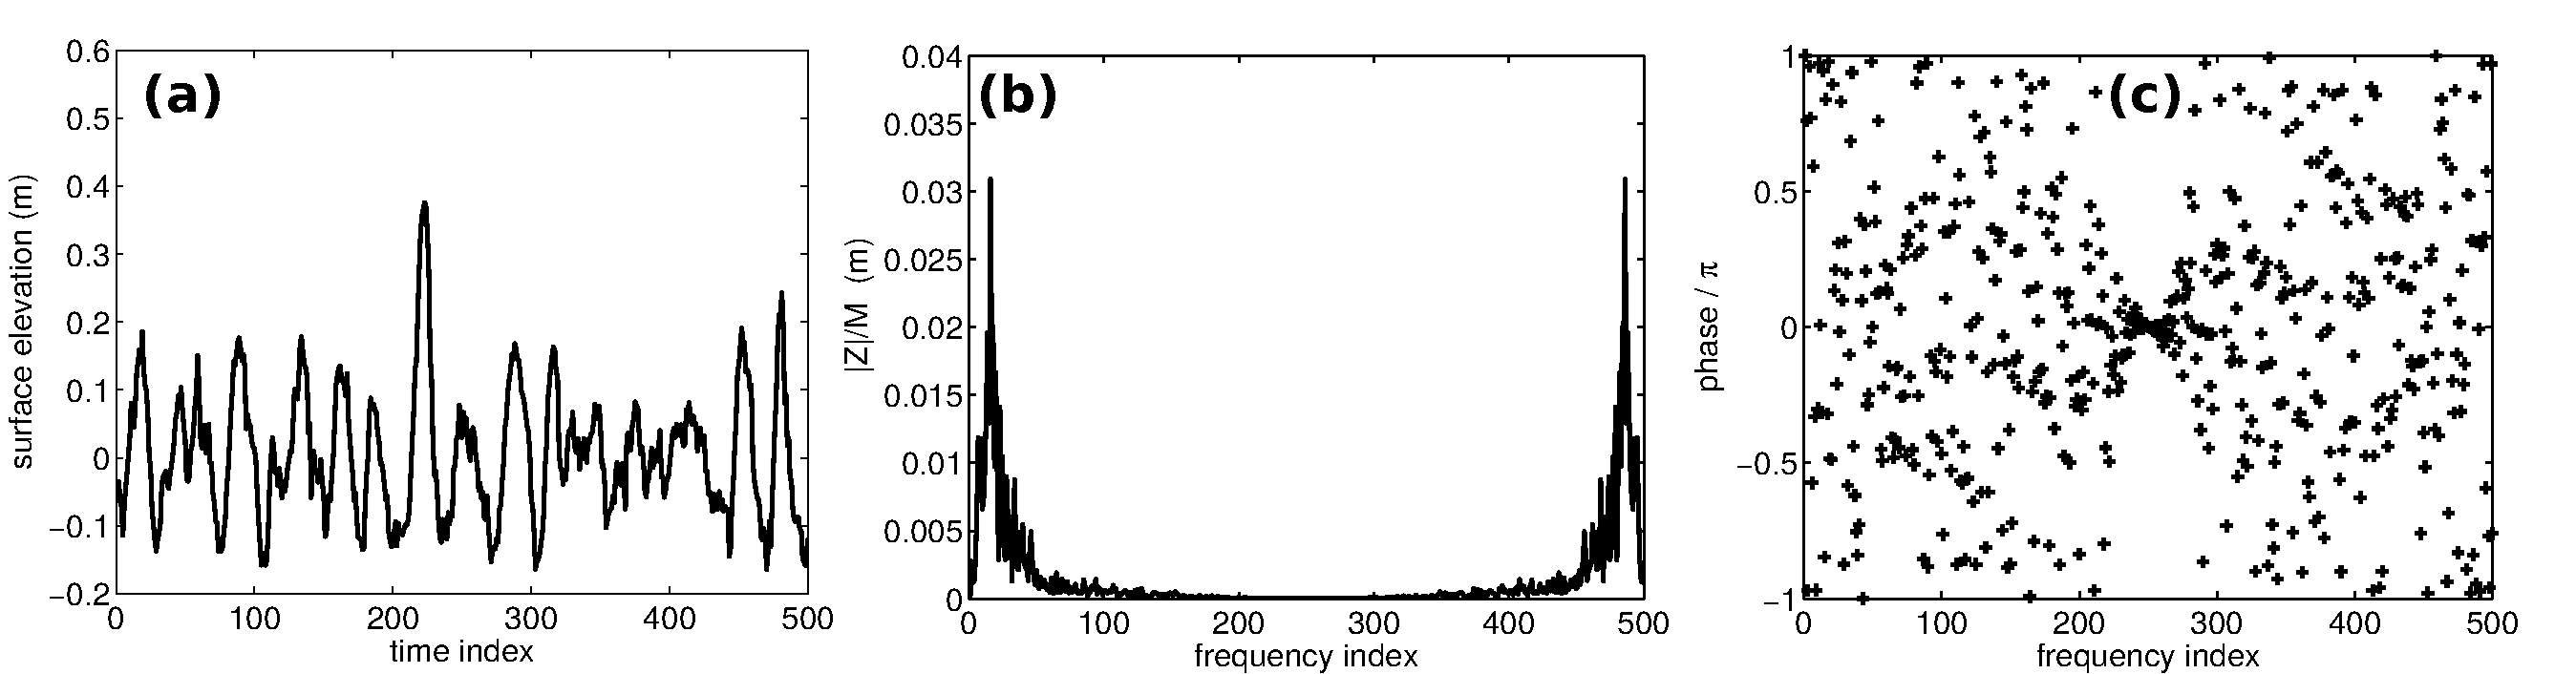
\includegraphics[width=0.9\textwidth]{FIGURES/spectra_DFT.pdf}}
%\vspace{3.64in}
\caption{(a) Example of surface elevation time series sampled at 12~Hz, (b) Discrete Fourier transform amplitude of the signal, and (c) phase of the same signal.} \label{fig:anaspec:spectreDFT}
\end{figure}
%%%%%%%%%%%%%%%%%%%%%%%%%%%%%%%%%%%%%%%%%%%%%%%%%%%%%%%%%%%%%%%%%%%%%%%%%%%%

With the definition given by eq. (\ref{eq:Zm_def}),  $Z_m=
\overline{Z_{M+2-m}}$, where the overbar is the complex conjugate, so that the modululs of the spectrum is symmetric around  $m=M/2$. This index $M/2$ corresponds to the Nyquist frequency 
$f_N=f_s/2 = M/2 df$. The symmetry means that above $f_N$ there is no new information. In other words, $f_N$ is the highest resolvable frequency. At this Nyquist frequency, a cosine wave is only represented by 2 points over a period. 

%We note that for stationary random variables that are quadratically integrable, i.e. all practical physical signals, the ratio $dZ(m) \overline{dZ(m)} / df$ goes to %$F(f)$ when $M$ goes 
%to infinity, i.e.  $f_s$ goes to zero, provided that  we keep constant 
%$f=(m-1)f_s/N$.  The increment
%$df=f_s/(N-1)$ is the spectral resolution, namely the frequency difference that can be resolved. The inverse of this resolution 
%$1/df$ is equal to the length of the recorded signal.

The continuous spectral density   $F(f)$ is obtained in the limit when the spectral resolution $df$ goes to zero of the following expression
\begin{equation}
    F(f=(m-1)f_s/M)  = 2  \frac{Z_m \overline{Z_m}}{df}.
\end{equation}
The factor 2 comes from the combination of positive and negative frequencies in the interval  $[0,  f_N]$. That definition is 
called the  single-sided spectrum. For some applications it may be convenient to keep the double-sided spectrum defined without this factor 2, 
for $f$ in the range $[0 , 2 f_N]$ or $[-f_N ,  f_N]$. 
In practice, the zero spectral resolution is never achieved because it corresponds to an infinitely long record. We are therefore stuck to finite 
spectral resolutions $df$, and thus a discrete spectrum sampled at $df$, corresponding to record lengths over which the random variable of interest is stationary. 


\subsection{Co-spectra}
In the same manner, we can  define the co-spectrum of two variables $a$ and $b$ having Fourier transforms $dA$ and $dB$, 
\begin{equation}
    C_{ab}(f=(m-1)f_s/M)  = \frac{A_m \overline{B_m}}{df} = P(f) +\mathrm{i}Q(f),
\end{equation}
where $P$ and $Q$ are real numbers, the co-spectra in phase and quadrature. 

We note that the product of two Fourier transforms is the Fourier transform of the convolution of the two functions. When these two functions are the same,
this result tells us that the spectrum is the Fourier transform of the auto-correlation function. When the two functions are different, the co-spectrum
is the Fourier transform of the correlation function. 

\section{Spectra from time series}
\subsection{Filtering of data and aliasing}
For any physical
parameter, the complex amplitude at a frequency above $f_N$ is the complex conjugate of the amplitude at a frequency below $f_N$: $dZ(N-m)=\overline{dZ(m)}$. 
In other words, the energy above the Nyquist frequency is aliased at  lower frequencies. This is one reason for applying a low-pass filter before the Fourier transform, in order to remove signals that would otherwise be aliased. 


%Il faut toujours bien r�fl�chir � la mani�re dont les donn�es sont filtr�es avant leur 
%�chantillonnage. Quand on mesure des vitesses toutes les dix minutes, est-ce une mesure instantan�e 
%une moyenne sur une, deux ou dix minutes? En effet les vitesses mesur�es contiendront alors 
%le courant moyen (par exemple caus� par la mar�e) mais aussi, si aucune moyenne n'est faite, les 
%fluctuations associ�es aux vagues et qu'il peut �tre tr�s d�licat de supprimer a post�riori. 

For example, a signal of period 1~s sampled every second ($f_s = 1$~Hz) is constant.  In general, any signal with frequency higher 
than the Nyquist frequency gives an apparent frequency in the range 
$[0 f_s/2]$, with a value obtained by folding back the spectrum along a vertical line at  $f=f_s/2$ or $f=0$ as many times as necessary, until 
 falling in $[0 f_s/2]$. Figure \ref{aliasing} shows an example of a true signal (in red) with frequency at  9/10 which gives  1-9/10=1/10 by aliasing. 
This is well known problem in oceanography in the case of the measurement of tides from satellite data. 
In the case of ocean waves, it is really necessary to measure waves with a sampling frequency that is at least 4 times the dominant frequency.  
%%%%%%%%%%%%%%%%%%%%%%%%%%%%%%%%%%%%%%%%%%%%%%%%%%%%%%%%%%%%%%%%%%%%%%%%%%%%
\begin{figure}[htb]
\centerline{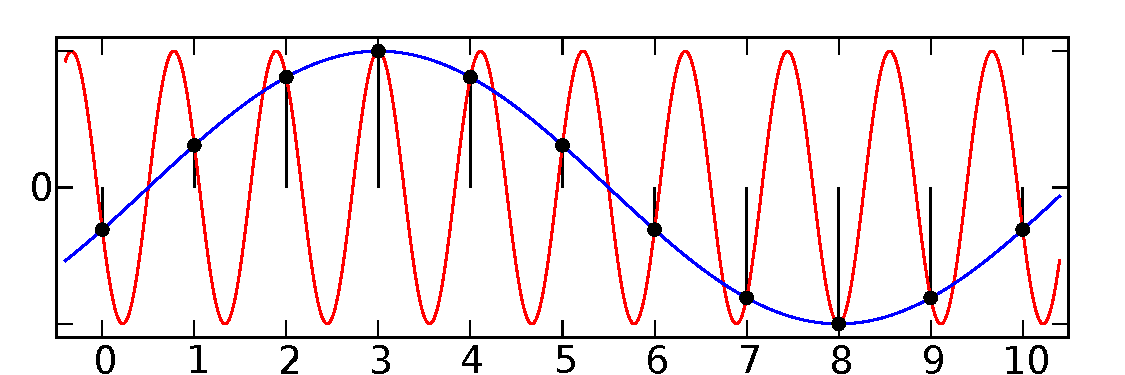
\includegraphics[width=0.5\textwidth]{FIGURES/AliasingSines.pdf}}
%\vspace{3.64in}
\caption{Example of spectral aliasing. A signal with period 10/9, in red, and sampled with a step of 1 (black dots) 
gives an apparent period of  10, in blue. (Moxfyre, wikimedia commons).} \label{aliasing}
\end{figure}
%%%%%%%%%%%%%%%%%%%%%%%%%%%%%%%%%%%%%%%%%%%%%%%%%%%%%%%%%%%%%%%%%%%%%%%%%%%%

In practice the high frequency roll-off of the wave spectrum, for $f > f_p$ in particular for pressure or velocity at the ocean floor, means that this 
filtering may not be necessary for the surface elevation. 
Figure \ref{fig:anaspec:timeseries} shows an example of the filtering of a surface elevation record and its impact on the spectrum. Here the filter helps in reducing 
the noise associated with the measurement method. 
%%%%%%%%%%%%%%%%%%%%%%%%%%%%%%%%%%%%%%%%%%%%%%%%%%%%%%%%%%%%%%%%%%%%%%%%%%%%
\begin{figure}[htb]
\centerline{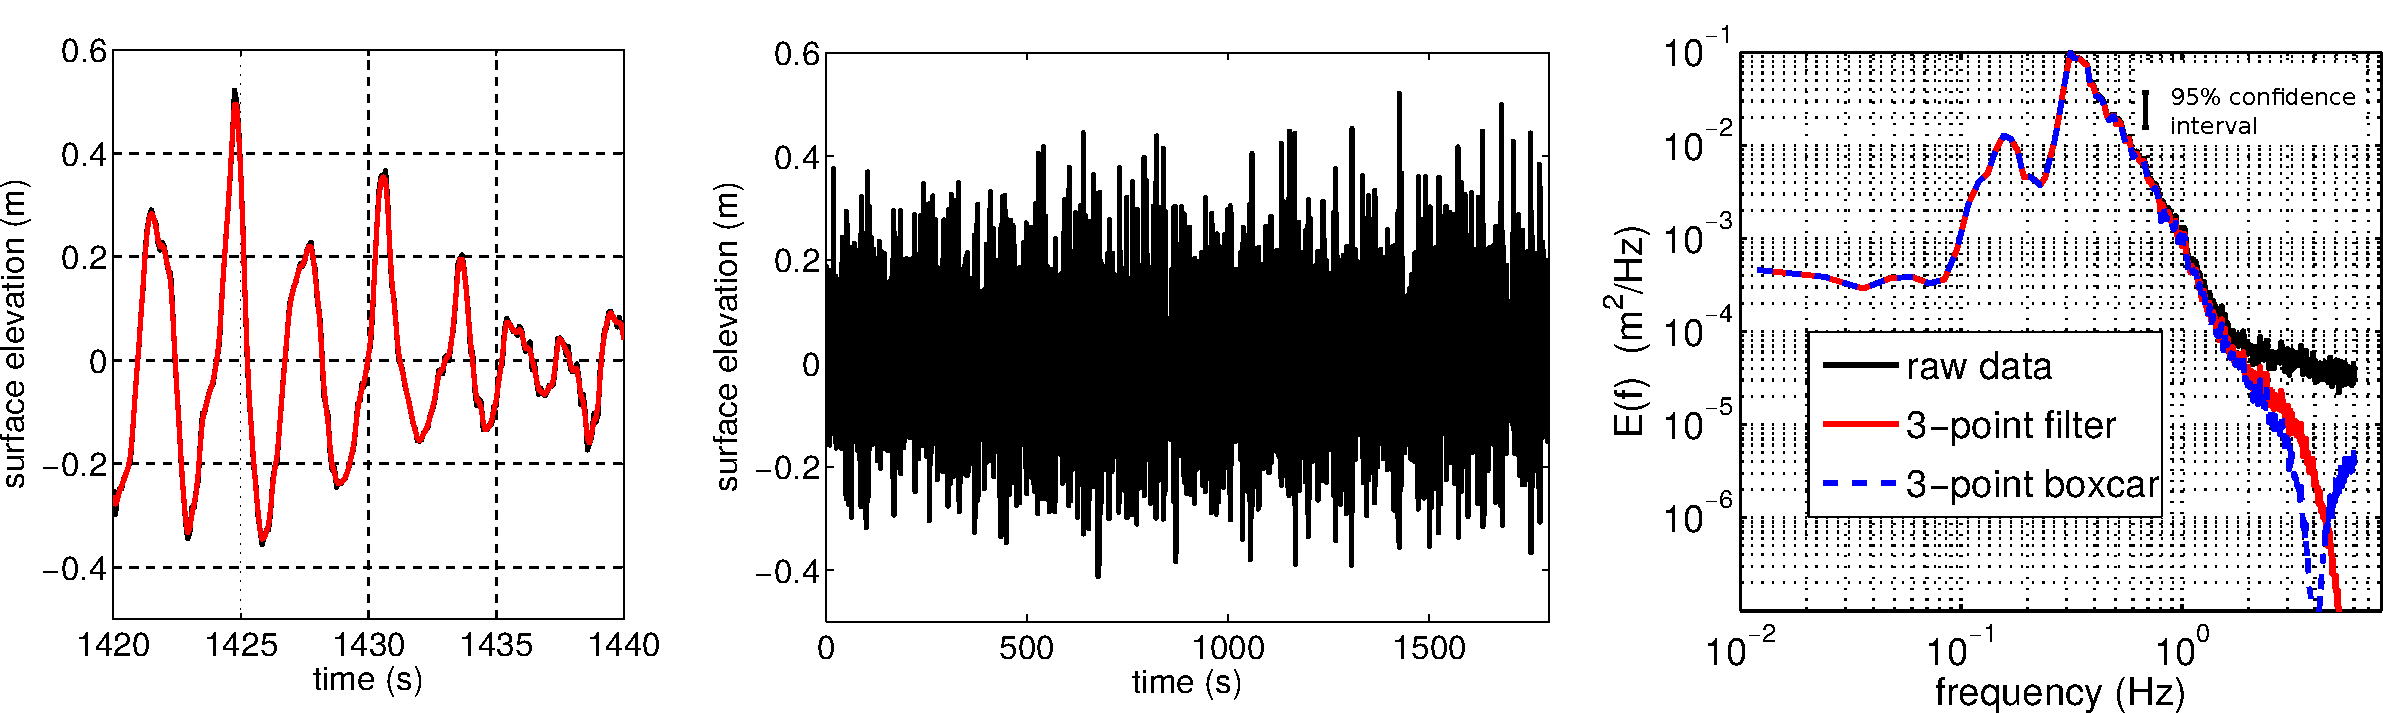
\includegraphics[width=\textwidth]{FIGURES/timeseries.pdf}}
%\vspace{3.64in}
\caption{Example of surface elevation measured by stereo-video from the Katsiveli platform, in 20~m depth, on Octoebr 4, 2011 \citep[see][for further detailed analysis of this dataset]{Leckler&al.2015,Aubourg&al.2017}.  (a) small piece of record around $t= 1430~s$ with (red) and without (black) a 3-point smoothing filter  (b) full record (1780~s) (c) spectra of the time series with different filters applied.} \label{fig:anaspec:timeseries}
\end{figure}
%%%%%%%%%%%%%%%%%%%%%%%%%%%%%%%%%%%%%%%%%%%%%%%%%%%%%%%%%%%%%%%%%%%%%%%%%%%%
The worst filter is clearly the boxcar (or moving average) filter with equal weight given to the consecutive data values, this does not suppress very well the shortest components.  


\subsection{Windows, Gibbs phenomenon and averaging}
The discrete Fourier transform of signal $\zeta$ that takes values at locations 1 to N, corresponds to the Fourier transform of a periodic signal that would 
repeat itself with $\zeta(n+m M) = \zeta (n)$ for any $n$ and $m$. If 
$\zeta(1)\neq \zeta(M)$, then this periodic function has a sharp jump from $\zeta(M)$ to $\zeta(M+1)$. Such a jump 
can give a strong spectral signature, all across the spectrum. 


This artifact is known as the Gibbs phenomenon, and it 
is generally removed by multiplying the signal  $\zeta(n)$ by a window function $W(n)$ which goes to zero or very small values for both 
$n=1$ and $n=N$. Obviously the spectrum of $\zeta(n) \times W(n)$ is different from the spectrum of $\zeta(n)$. The first obvious effect is that 
the variance of the signal has been reduced by a factor that is the average of $W^2$. That is easily corrected for.




Let use the time series shown in figure \ref{fig:anaspec:timeseries}.b. We first start with a small piece of only 1000 points. The original time series, in black 
in figure \ref{fig:anaspec:spectre1}.a gives the power spectral density in figure {fig:anaspec:spectre1}.b. If the time series is brought to zero at both ends (in red) by multiplying with a Hann window, then the spectrum is transformed. However, because of the random fluctuations of the spectral estimates this is not obvious.
Indeed waves are random and the surface elevation is nearly-Gaussian. As a result, the complex Fourier amplitudes are also random and Gaussian, so that they modulus, which is the power spectral density has the shape of a  $\chi^2_n$ distribution with $n=2$ degrees of freedom. Because the $\chi^2_n$ distribution has a mean of $n$, the distribution of estimates $\widehat{E}(f)$ of the spectrum, once normalized by the mean spectrum $E(f)$ follows the rescaled $\chi^2_n$ disitribution, with a mean equal to 1. 

%%%%%%%%%%%%%%%%%%%%%%%%%%%%%%%%%%%%%%%%%%%%%%%%%%%%%%%%%%%%%%%%%%%%%%%%%%%%
\begin{figure}[htb]
\centerline{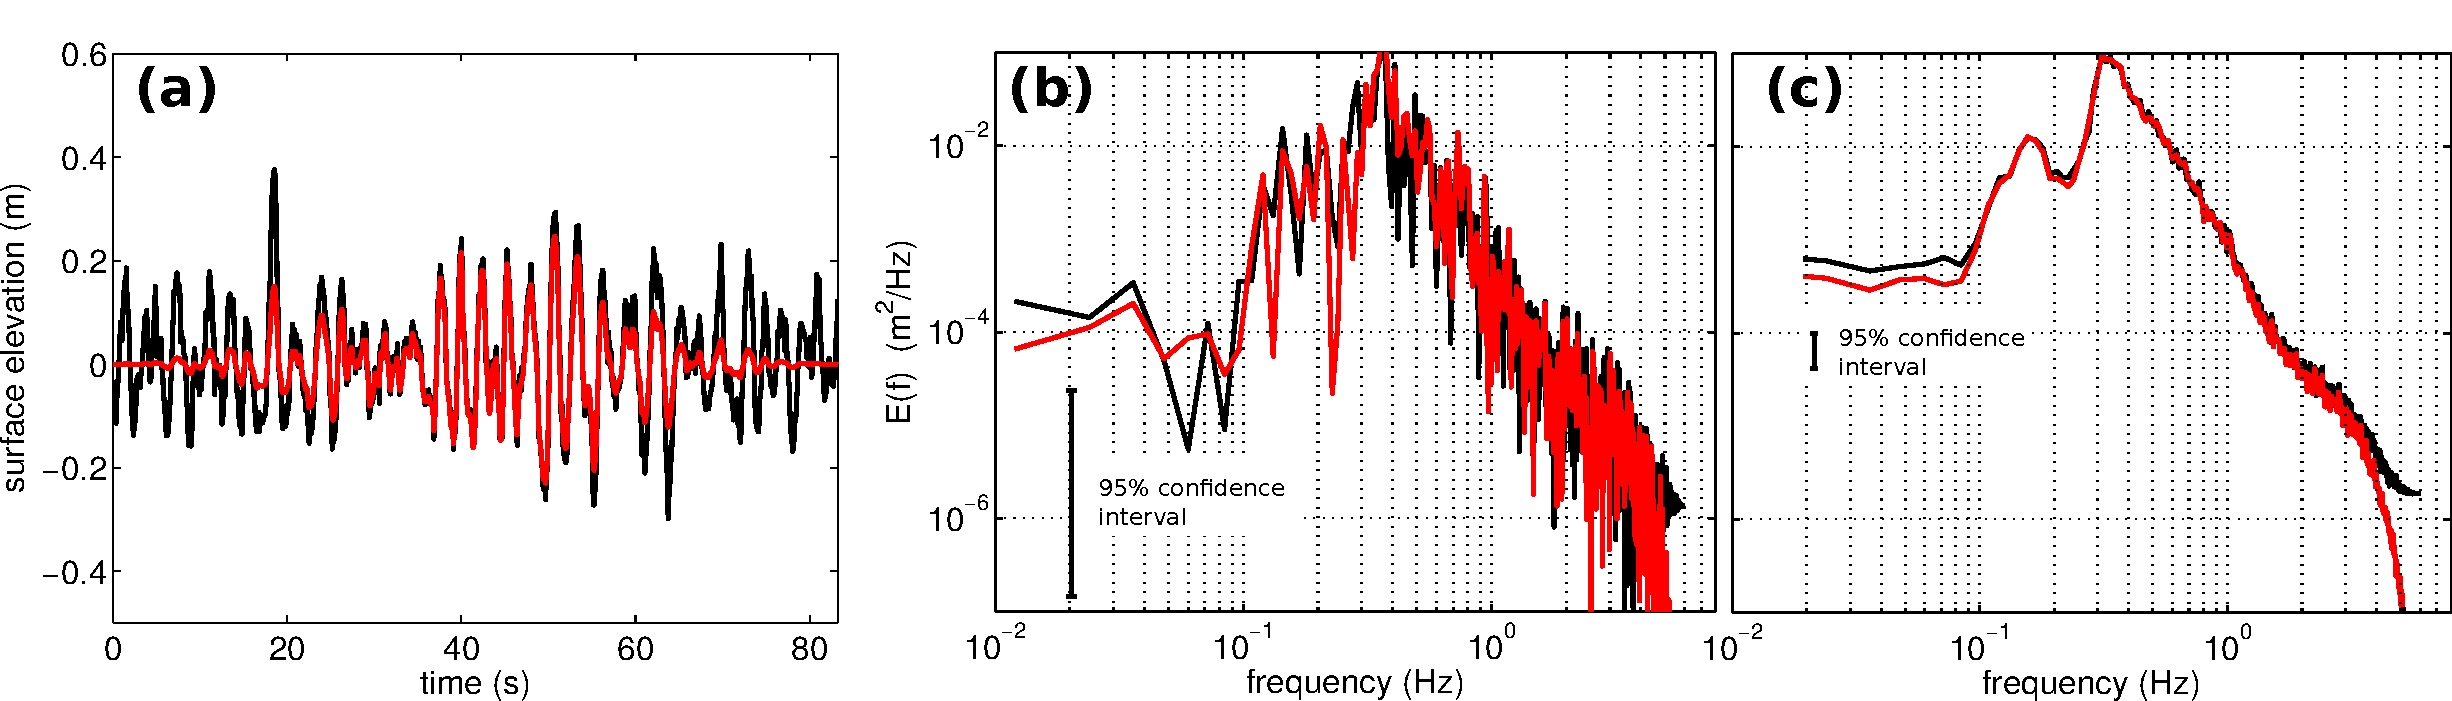
\includegraphics[width=\textwidth]{FIGURES/spectra1.pdf}}
%\vspace{3.64in}
\caption{(a) First 1000 points of time series shown in  (\ref{fig:anaspec:timeseries}).b, with (red) and without (black) multiplication by a Hann window. 
(b) Resulting spectra (c) Average spectra using Welch's method with 21 independent windows and thus 42 degrees of freedom.} \label{fig:anaspec:spectre1}
\end{figure}
%%%%%%%%%%%%%%%%%%%%%%%%%%%%%%%%%%%%%%%%%%%%%%%%%%%%%%%%%%%%%%%%%%%%%%%%%%%%
 Using figure \ref{table_chi2}, we find that the expected ratio of the lower and upper bound of a 95$\%$ confidence interval is 146. This number is the ratio of  $\chi^2_{2,0.975}$�and  $\chi^2_{2,0.025}$, that give the probabilities that $\chi^2_{n} > \chi^2_{n,\alpha}$ is equal to the acceptance threshold $\alpha$. 
%%%%%%%%%%%%%%%%%%%%%%%%%%%%%%%%%%%%%%%%%%%%%%%%%%%%%%%%%%%%%%%%%%%%%%%%%%%%
\begin{figure}
\centerline{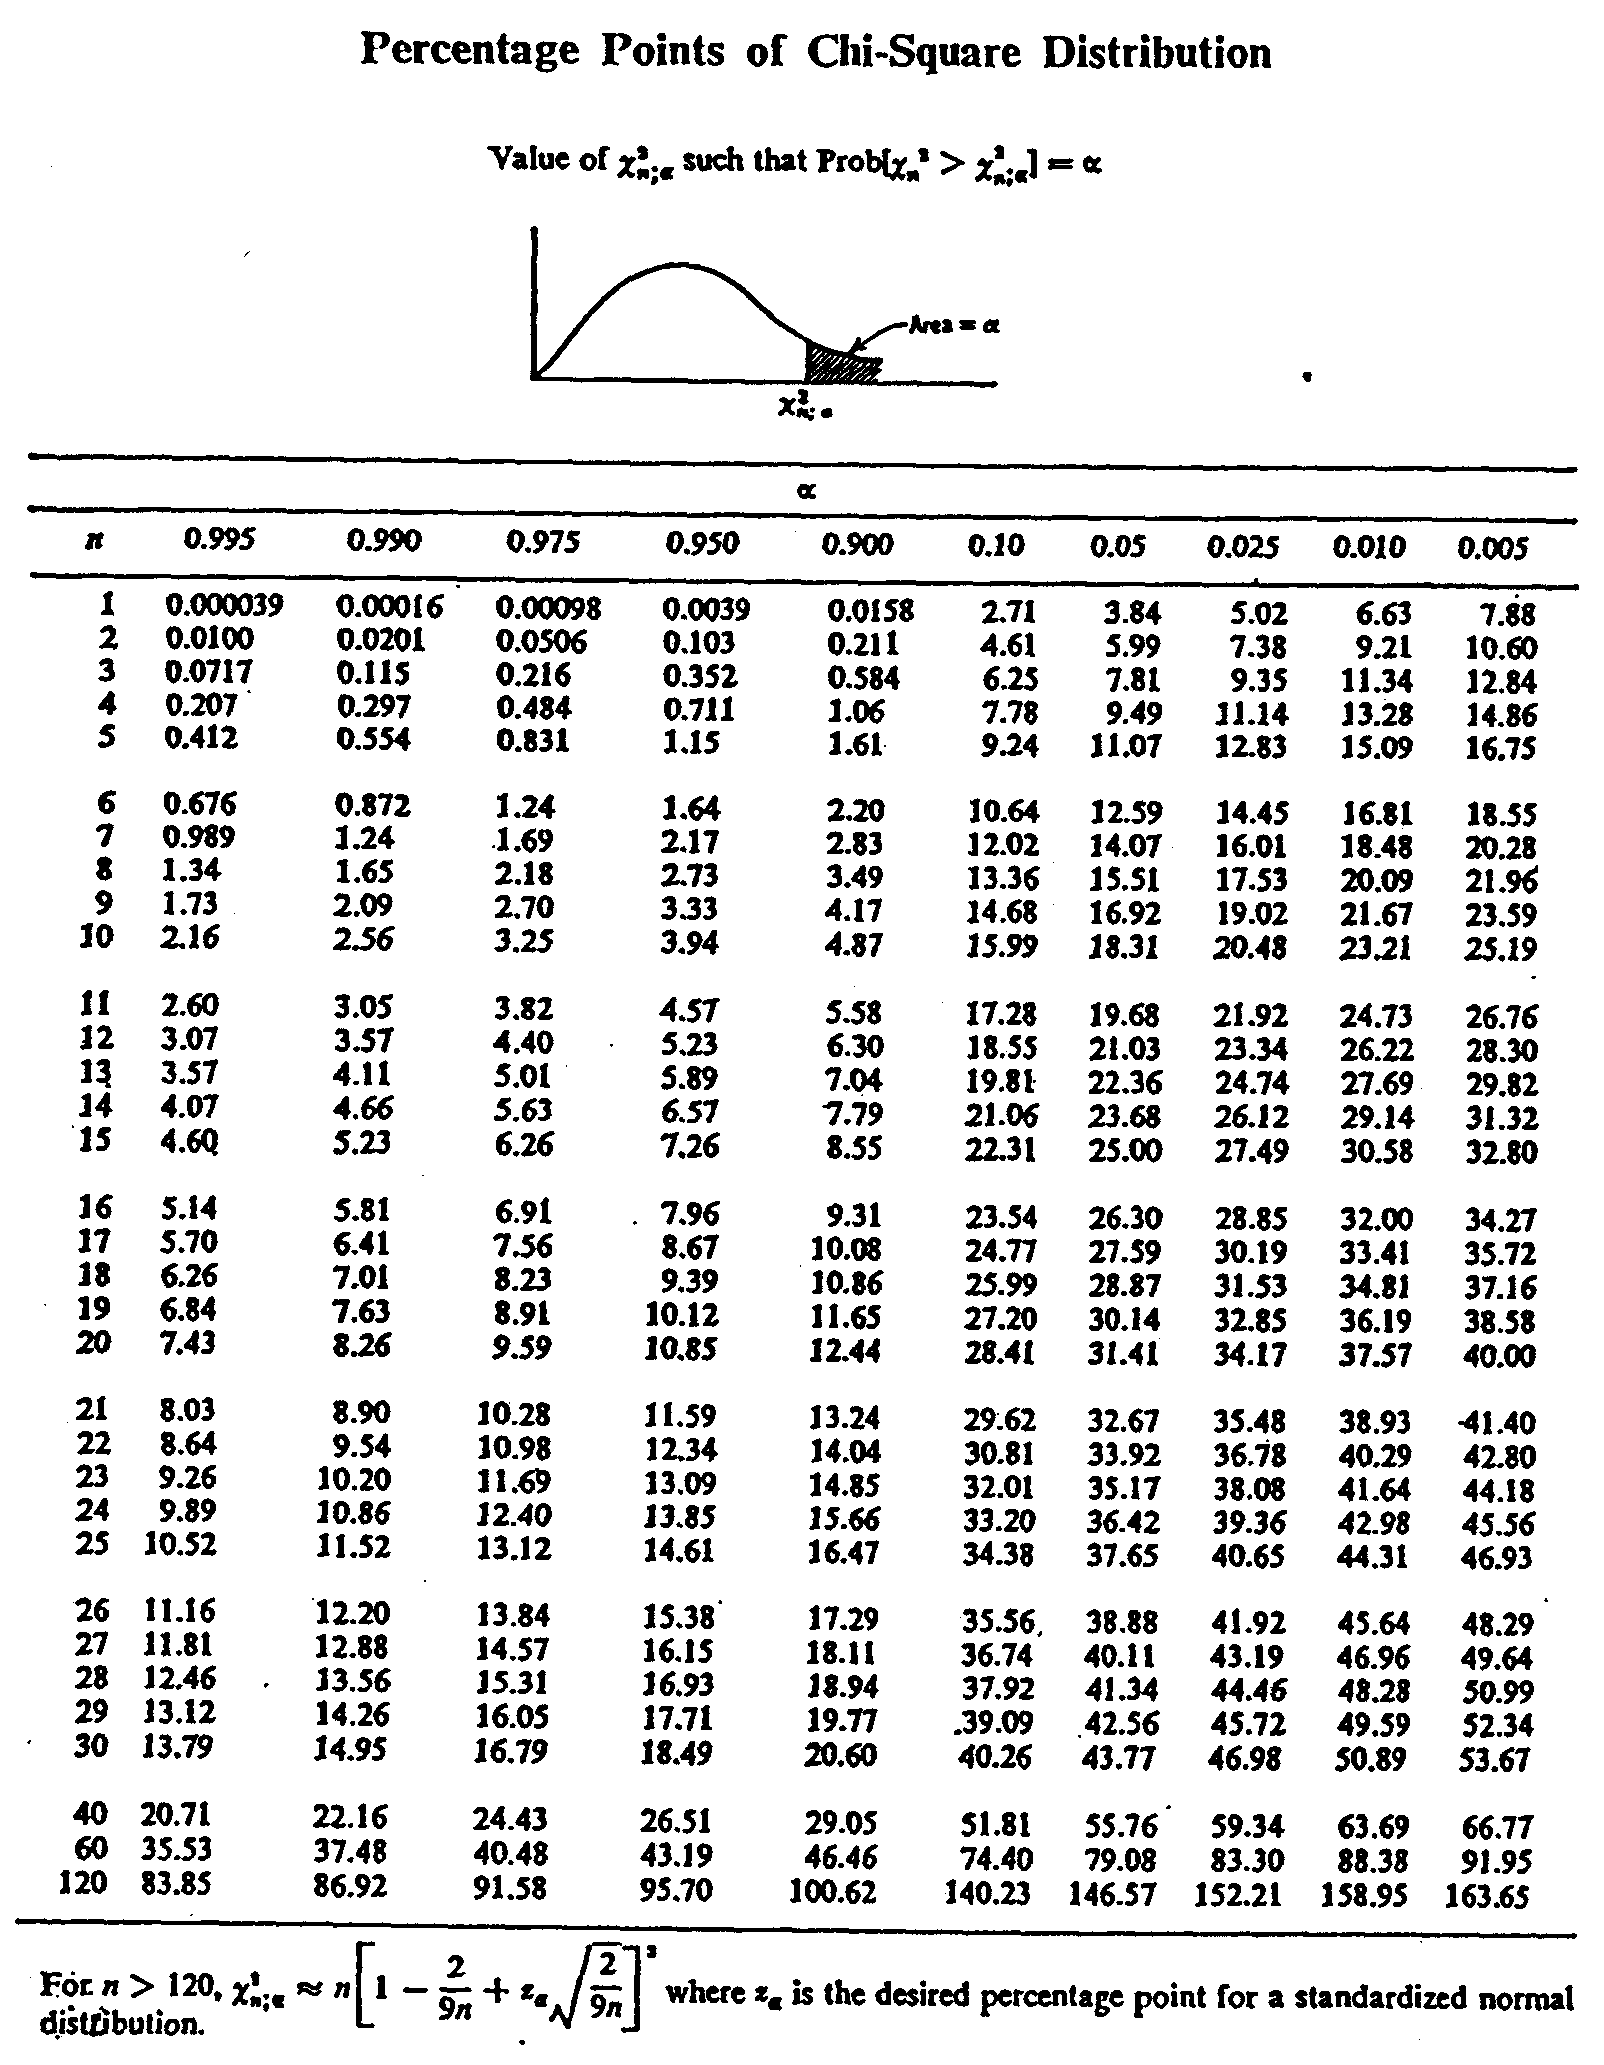
\includegraphics[width=\textwidth]{FIGURES/table_chi2.png}}
%\vspace{3.64in}
\caption{Table of $\chi^2$ distributions. This table gives the confidence intervals
for the estimation of spectra with 
$n=2 N$ degrees of freedom, where $N$ is the number of independent spectra used.} \label{table_chi2}
\end{figure}
%%%%%%%%%%%%%%%%%%%%%%%%%%%%%%%%%%%%%%%%%%%%%%%%%%%%%%%%%%%%%%%%%%%%%%%%%%%%


For an expected value  $\widehat{E}$, the  Gaussian statistics theory predicts a 95\% probability that the estimate of $E(f)$ is in the range $[E_1, E_2]$ with $E_1=\widehat{E} \times 0.0506/2 $ and  $E_2=\widehat{E} \times 7.38/2$, where 0.0506 and 7.38 are the values for which the $\chi^2$ cumulative probability function for 2 degrees of freedom is $\alpha=0.975$ and $\alpha=0.025$, respectively as given \ref{table_chi2}. In other words, the random fluctuations of the spectrum estimated by a single Fourier transform spans more than two orders of magnitude. 

That is fairly annoying. There are two ways to reduce this uncertainty: the first, which is most easily done in the laboratory is to run more experiments, repeating the same conditions, with random wave phases, and average the results. For measurements in the field, this is the same as processing a longer time series, but it only makes sense if the conditions are stationary: same wind, same wave age, same current, etc. In practice, this stationarity constraints limits the length of records from half an hour to a few hours. As we average $N$ spectra together, the number of degrees of freedom increases to $2N$. Here we have used 21 independent spectra, and we get an uncertainty that narrows like $1/\sqrt{N}$ for large $N$. For 20 spectra, the ratio $E_2/E_1$ is $59.34/34.43\simeq 1.7$. As $N$ increases, the spectral resolution becomes coarser.

Because the Hann window practically removes part of the data, \cite{Welch1967} has defined a method in which the windows are shifted by half their length, as shown in figure \ref{fig:anaspec:spectre31}.a. The lower panel shows the 21+20 spectra estimated, and the average result.  
%%%%%%%%%%%%%%%%%%%%%%%%%%%%%%%%%%%%%%%%%%%%%%%%%%%%%%%%%%%%%%%%%%%%%%%%%%%%
\begin{figure}
\centerline{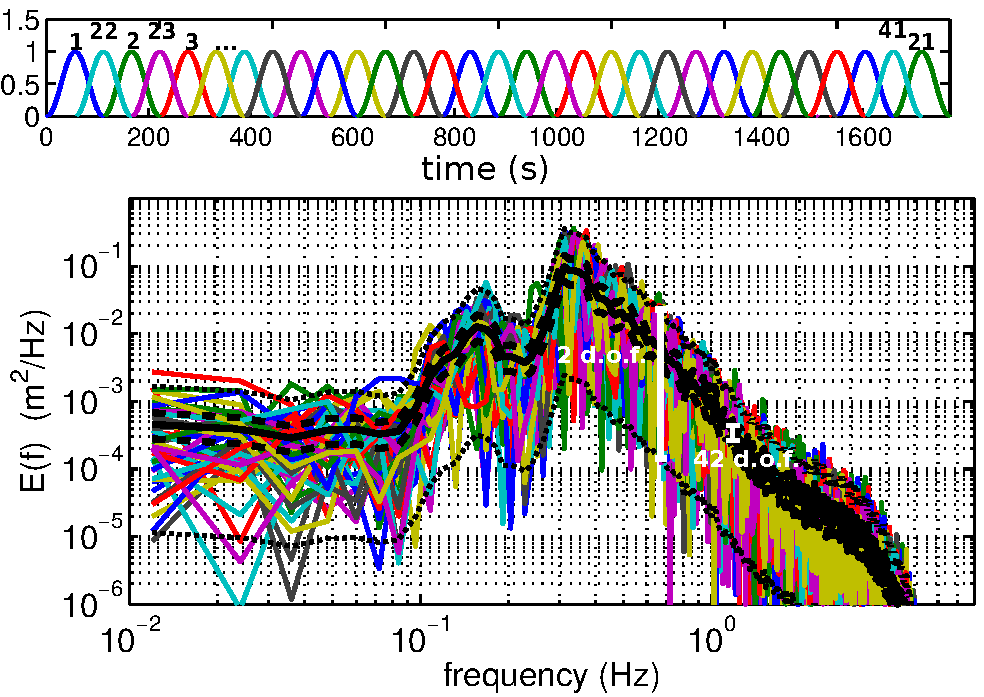
\includegraphics[width=0.9\textwidth]{FIGURES/spectra_31.pdf}}
%\vspace{3.64in}
\caption{(a) Succession of the Hann windows applied to the data, with 21 independent windows and 20 overlapping windows, from number 22 to 41. The solid line is the mean spectrum and the dotted and dashed line show the expected 95\% confidence intervals for 2 and 42 degrees of freedom. 
� 95\%.} \label{fig:anaspec:spectre31}
\end{figure}
%%%%%%%%%%%%%%%%%%%%%%%%%%%%%%%%%%%%%%%%%%%%%%%%%%%%%%%%%%%%%%%%%%%%%%%%%%%%

Another method that is almost equivalent to Welch's is the smoothing of the spectrum, also known as band-averaging. Because the Fourier transform of a shorter 
window has a coarser resolution, both methods effectively trade off the spectrum accuracy against the spectral resolution. An extension of such methods is the use of wavelet transforms \citep[e.g.][]{Liu&Babanin2004} which aims at localizing events in both time and frequency. 

Whatever the choice of method, without any prior knowledge on the signal, the product of the spectra uncertainty and the square root of the frequency uncertainty remains constant. Thus the optimal choice of $df$ is up to the user. For wind seas, the typical relative width of the spectrum is 0.1, and for a typical peak period of 0.1~Hz, resolving the peak requires $df < 0.01$~Hz. For swells one may like to have an even narrower frequency resolution.  In the example above, $df=0.012$~Hz is 
enough for the relatively short wind sea found in the Black Sea. 

\subsection{Interpretations and further developments}
The general idea of spectral analysis is to decompose a signal into its basic constituents. If waves were indeed linear, the Fourier components would be truly independent and the spectrum would give the energy of different wave components. In practice, there is a significant level of nonlinearity, which actually dominates the frequency spectrum $E(f)$ at frequencies above 3 to 4 times the wind sea peak \citep[e.g.][]{Leckler&al.2015}. As a result, the interpretation of these high frequencies ($f > 1$~Hz in the example above) as the energy of linear waves is wrong. Several methods have been developed to try to separate linear and non-linear components, including higher order analysis \citep{Hasselmann&al.1963} which is illustrated in chapter \ref{ch_surf}. This question has inspired other nonlinear methods, such as the Empirical Mode Decomposition method by \cite{Huang&al.1998}.


\section{Spectral analysis of directional buoy data}
\subsection{Case of 3-axis displacements or accelerations}
We have seen in section  \ref{sub:transfer} that the spectrum of $x$-component velocity  at the ocean bottom 
is given from the surface elevation spectrum multiplied by a transfer function,
\begin{equation}
    E_{Ux} \left( f,\theta \right)  = \frac{\sigma^2 \cos^2 \theta}{\sinh^2 (kD)} E\left( f,\theta
    \right)\label{EUX }.
\end{equation}
%et le module moyen de la vitesse (en moyenne quadratique) pr�s du fond vaut,
%\begin{equation}
%    U_{\mathrm{b,rms}} = \left[\int_0^{\infty} \int_0^{2 \upi} \frac{\sigma^2}{\sinh^2
%    (kD)} E\left( f,\theta \right){\mathrm d}\theta
%    {\mathrm d}f \right]^{1/2}
%\end{equation}

The same method applies to spectra of displacements, velocity and slopes at the sea surface. 
For a water particle at the surface, the spectra of displacement in the three directions are given by  (\ref{xi3}),
\begin{eqnarray}
    E_{x} ( f)  & = &  \frac{1}{\tanh^2(kD)} \int_0^{2 \upi} E\left( f,\theta \right)\cos^2 \theta {\mathrm
    d}\theta \\
    E_{y} ( f)  & = &  \frac{1}{\tanh^2(kD)} \int_0^{2 \upi} E\left( f,\theta \right)\sin^2 \theta {\mathrm
    d}\theta \\
   E_{z} ( f)  & = &  \int_0^{2 \upi} E\left( f,\theta \right) {\mathrm
    d}\theta.
\end{eqnarray}
We note that this last spectrum is the usual elevation spectrum $E(f)$, also called heave spectrum, with a minor modification due to the fact that it is not 
obtained at a fixed position $(x,y)$ but at a positions that moves with $x$ and $y$. As a result, the shape of the waves and the shape of the spectrum are modified, with a strong reduction in the contribution of nonlinear harmonics: a surface buoy signal looks much more linear than a wave staff or stereo video record. 

The co-spectra of horizontal and vertical displacements are 
\begin{eqnarray}
    C_{xz} ( f)  & = &  \frac{\mathrm i}{\tanh(kD)} \int_0^{2 \upi} E\left( f,\theta \right)\cos \theta {\mathrm
    d}\theta, \label{Exz}\\
    C_{yz} ( f)  & = &  \frac{\mathrm i}{\tanh(kD)} \int_0^{2 \upi} E\left( f,\theta \right)\sin \theta {\mathrm
    d}\theta .\label{Eyz} \\
    C_{xy} ( f)  & = &  \frac{1}{\tanh^2(kD)} \int_0^{2 \upi} E\left( f,\theta \right)\sin \theta \cos \theta {\mathrm
    d}\theta .\label{Exy}
\end{eqnarray}
These co-spectra are thus related to the mean direction and directional spread, through the directional moments introduced in section  \ref{sub:param}
\begin{eqnarray}
    a_1 ( f)  & = &  \int_0^{2 \upi} E\left( f,\theta \right)\cos \theta {\mathrm
    d}\theta, \\
    b_1 ( f)  & = &   \int_0^{2 \upi} E\left( f,\theta \right)\sin \theta {\mathrm
    d}\theta,  \\
    a_2 ( f)  & = &  \int_0^{2 \upi} E\left( f,\theta \right)\cos (2\theta) {\mathrm
    d}\theta, \\
    b_2 ( f)  & = &   \int_0^{2 \upi} E\left( f,\theta \right)\sin (2 \theta) {\mathrm
    d}\theta.
\end{eqnarray}


To summarize, starting from the displacement time series  $x(t)$, $y(t))$ and $z(t)$ one obtains the 
spectra and co-spectra  $C_{xx}(f)$,  $C_{yy}(f)$,  $C_{zz}(f)$,  $C_{xz}(f)$, $C_{yz}(f)$ , $C_{xy}(f)$.
Using $\cos(2 \theta)=\cos^2(\theta) - \sin^2(\theta)$ and $\sin(2 \theta)=2 \sin \theta \cos\theta$, they give the following directional moments, in which $\Im $ stands for the imaginary part, 
\begin{eqnarray}
  a_1 ( f) &=&-\Im (C_{xz}(f))/\left[C_{zz}(f) \left(C_{xx}(f)+C_{yy}(f)\right)\right] \\
  b_1 ( f) &=&-\Im (C_{xy}(f))/\left[C_{zz}(f) \left(C_{xx}(f)+C_{yy}(f)\right)\right] \\
  a_2 ( f) &=&(C_{xx}(f)-C_{yy}(f))/(C_{xx}(f)+C_{yy}(f)) \\
  b_2 ( f) &=&2 C_{xy}(f) /(C_{xx}(f)+C_{yy}(f))  \\
\end{eqnarray}
from which we get directional parameters, with $\mod$ the modulo operator, 
\begin{eqnarray}
  \theta_{1}(f) &=&  \mod( 270.- \mathrm{atan2}(b1,a1)\times 180/\pi, 360)\\
  \sigma_{1}(f)&=&\left[2\left(1 - \sqrt{a_1^2(f) + b_1^2(f)} \right)\right]^{0.5}\times 180/\pi \\
  \theta_{2}(f) &=&  \mod( 270.- 0.5 \mathrm{atan2}(b2,a2)\times 180/\pi, 360)\\
  \sigma_{2}(f)&=&\left[0.5\left(1 - \sqrt{a_2^2(f) + b_2^2(f)} \right)\right]^{0.5}\times 180/\pi
\end{eqnarray}


These 4 parameters can be used in statistical estimators to obtain the directional spectrum $E(f,\theta)$. A commonly used estimator 
is the Maximum Entropy Method of \cite{Lygre&Krogstad1986}. See also the review by \cite{Benoit&al.1997}.

\subsection{Case of other systems with 3 variables or more}
in the above method, we can replace $x$ and $y$ by the slopes $\partial \zeta / \partial x$  and $\partial \zeta / \partial y$ as done in the pitch-and-roll buoys 
developed by \cite{Cartwright&Smith1964} and still widely used. For example, most of the 3-m discuss buoys operated by the U.S. National Data Buoy Center are based 
on this measurement \citep{Steele&al.1992}. Also, the horizontal 
velocities at any given level, $(u,v)$. These give access to the heave spectrum $E(f)$ and the same directional moments $a_1$, $b_1$, $a_2$ and $b_2$. 

In order to go beyond these first 5 parameters, one can built an array of instruments. The cloverleaf buoy of \cite{Mitsuyasu&al.1975} was such an attempt, and arrays of pressure gages or lasers have been routinely used. Today's optical techniques \citep{Benetazzo2006,Fedele&al.2013,Laxague&al.2015} are other ways to get to more details about the sea surface.


\section{Some links between spectral and wave-by-wave analysis}
The spectrum $E(f)$ gives the distribution of the surface elevation variance as a function of time scales. As discussed in chapter \ref{ch1}, one can also chop the 
signal in individual waves and study the statistics of their properties. 
A model for the sea surface elevation could be a signal of constant amplitude with a random frequency modulation. In that case, \cite{Woodward1952}'s theorem 
tells us that the spectrum of the signal is the distribution of its frequencies $P_f(f-f_c)$ where $f_c$ is the carrier frequency,
\begin{equation}
    E(f) = \frac{a^2}{2}P_f(f-f_c).
\end{equation}

Extension of that theorem by \cite{Blachman&McAlpine1969} with an additional amplitude modulation makes it applicable to ocean waves.  As  shown by  \cite{Elfouhaily&al.2003} the spectrum is then given by the joint probability distribution of wave heights and periods $P(a,f)$ with $a=H/2$ and $f=1/T$. 
Separating linear (naked) and full (dressed) spectra, \cite{Elfouhaily&al.2003} showed that the peak region is dominated by linear components 
\begin{equation}
    E_{\mathrm bare}(f) = \frac{1}{2}\int a^2 P(a,f) da.
\end{equation}

At high frequency the nonlinear contributions dominate the spectrum which can be interpreted as fast modulations of the short components. Taking into account that 
effect leads to asymetries $\alpha$ et $\beta$
(see figure \ref{Asymetrie_Elf}), and the dressed spectrum
\begin{equation}
    E_{\mathrm{dressed}}(f) =  E_{\mathrm nu}(f) +\frac{1}{2}\left[ \int \alpha^2 P(\alpha,f/2)
    da+ \int \beta^2 P(\beta,f/2) da\right] \simeq E(f)
\end{equation}
%%%%%%%%%%%%%%%%%%%%%%%%%%%%%%%%%%%%%%%%%%%%%%%%%%%%%%%%%%%%%%%%%%%%%%%%%%%%%%%%%%%%%
\begin{figure}
\centerline{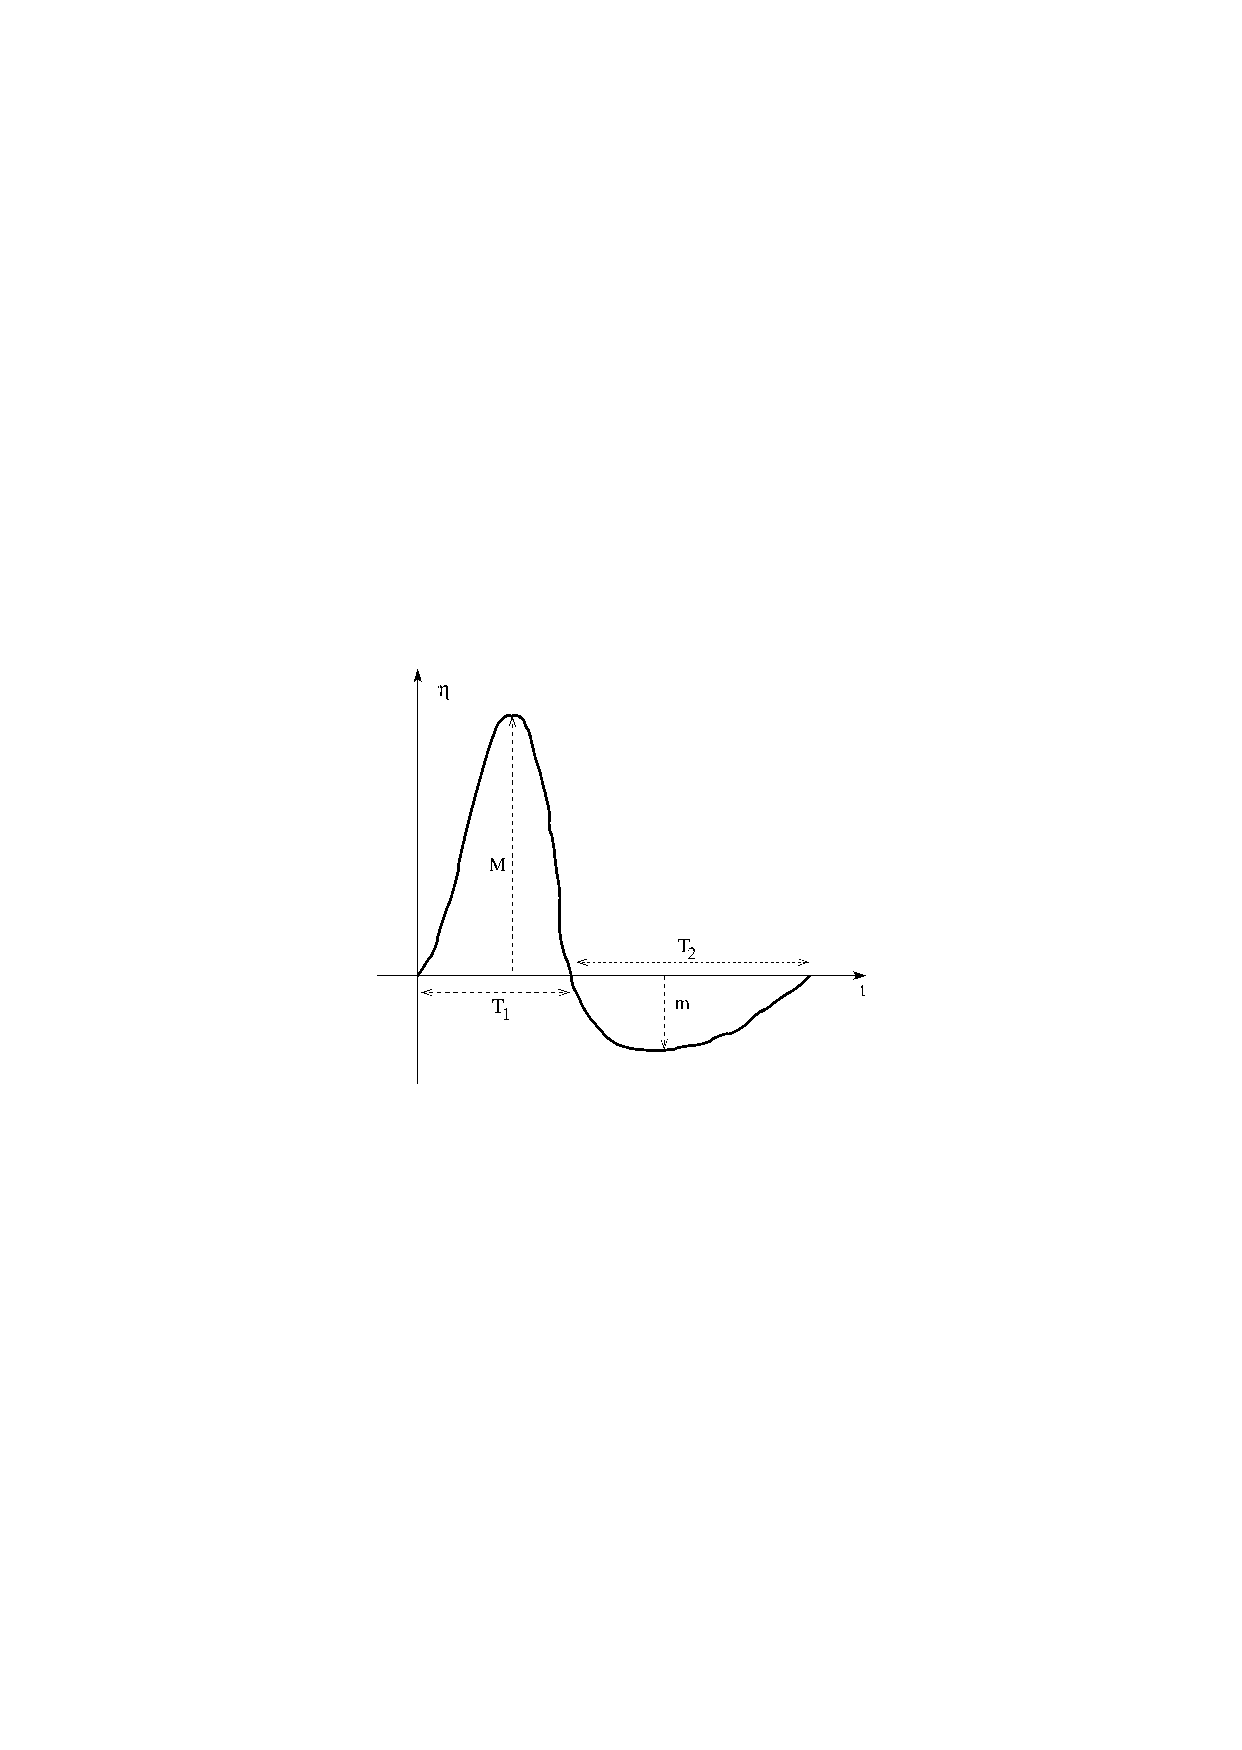
\includegraphics[width=0.6\textwidth]{FIGURES/Asymetrie_Elf.pdf}}
%\vspace{3.64in}
  \caption{Definition of parameters $M$ ,$m$, $T_1$ et $T_2$ used to estimate the amplitude  $a=(M-m)/2$, period $T=T_1+T_2$, vertical asymetry  $\alpha=(M+m)/2$  and horizontal asymetry $a\pi(T_1-T_2)/(T_1+T_2)/2$ (from \cite{Elfouhaily&al.2003}, \copyright Elsevier).
   Here $m<0$, because $m$ is defined as the trough level between two up-crossing zeros that define the start and end of the wave.} \label{Asymetrie_Elf}
\end{figure}
%%%%%%%%%%%%%%%%%%%%%%%%%%%%%%%%%%%%%%%%%%%%%%%%%%%%%%%%%%%%%%%%%%%%%%%%%%%%%%%%%%%%%%%%%%%



\cleardoublepage
\chapter{Wave groups and fluctuations of wave parameters}\label{ch_groups}
Before we look at the evolution of the wave field over tens of kilometers and hours time scale, it is 
worth looking at consequences of the shape of the wave spectrum 
on fluctuations in wave properties at the scale of few minutes and kilometers.
Indeed, the fact that waves are random introduces small scale variations. Most early work 
was focused on defining the statistics of series of high waves \citep{Arhan&Ezraty1978,Masson&Chandler1993}, which can be useful for example when catching 
waves on a surfboard, avoid the high waves when navigating a landing craft through the surf zone, or landing a helicopter on a ship. In this 
chapter we will start with another application which has become prominent as we are 
starting to look at smaller and smaller scale details in the wave field: estimating the expected 
fluctuations associated with groups \citep{DeCarlo&al.2023}, so that we may separate it from other effects, including 
refraction induced by currents and water depth, wave breaking, etc, which will be discussed in the 
following chapters. This investigation will also allow us to estimate lower bounds for uncertainties 
of wave measurements that will be defined from the time and space footprint of t{he measurements. The full uncertainty also contains instrument noise and measurement noise effects.

\section{Wave envelope, local amplitudes and their statistics}

Let $\zeta_c$ be the complex number such that $\zeta = \mathrm{Re}(\zeta_c)$ is the free surface, $\zeta_c$  is usally called the analytic signal. The envelope $\eta$ of the signal is defined by  $\eta = |\zeta_c|$, with an example shown in Fig. \ref{fig:groups1D}, using bottom pressure $p(z=-h)$ instead of surface elevation $\zeta$. 
%%%%%%%%%%%%%%%%%%%%%%%%%%%%%%%%%%%%%%%%%%%%%%%%%%%%%%%
\begin{figure}[htb]
\centerline{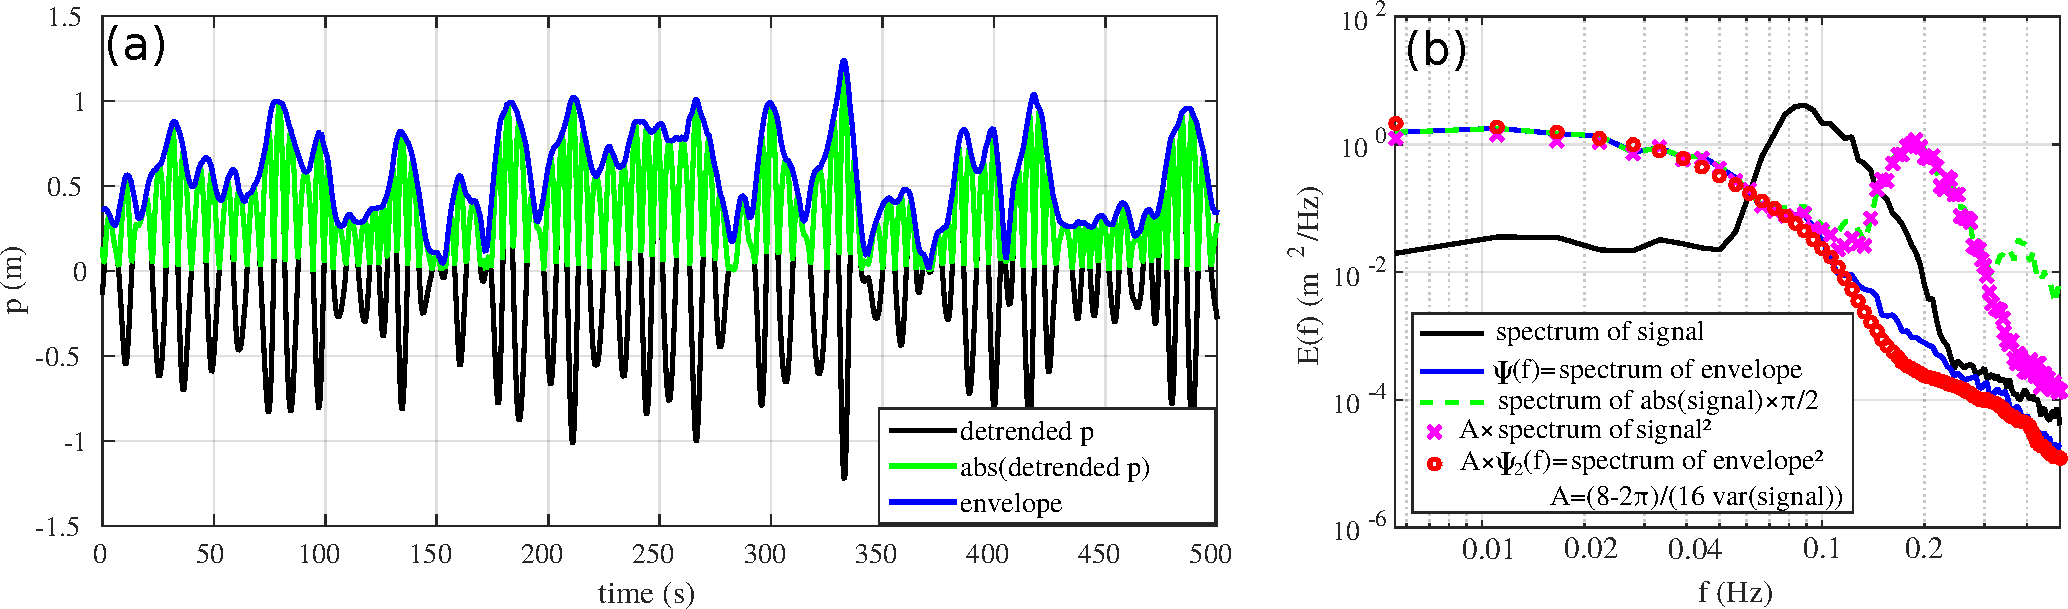
\includegraphics[width=\textwidth]{FIGS_CH_GROUPS/envelope_1D.pdf}}
%\vspace{3.64in}
  \caption{(a) time series of a signal, here the detrended ocean bottom pressure in Berthaume on January 31st 2004 (same data as in Figure 1.2), absolute value of the signal and signal envelope. (b) Spectra of the signal, the envelope, the rectified signal, and the approximate spectrum $\Psi_2$ obtained from a spectral convolution.}
\label{fig:groups1D}
\end{figure}
%%%%%%%%%%%%%%%%%%%%%%%%%%%%%%%%%%%%%%%%%%%%%%%%%%%%%%%
This defines a local amplitude of the signal that is continously defined everywhere. One interesting property of the envelope is that it does not contain the small scale crest-to-trough (positive to negative) variations of the original surface, so that its spectrum actually contains only longer components (larger periods in the case of time series). It is interesting to note that a similar operation is obtained by \emph{rectifying} the signal, i.e. taking its absolute value. This was particularly studied for electric signals by \cite{Rice1944} and the \emph{rectifier} in that case is a simple diode bridge. In the case of ocean waves, an important application is that of forces on moored ships, and you can think of the mooring line as a kind of rectifier, which will thus endure low-frequency forces. 

In fact it is easy to show that the signal and the rectified signal have the same mean squared value (i.e. the same integral of the spectrum including $f=0$), but they have very different spectra: the mean squared of the rectified signal is actually split half and half between sub-harmonics (very low frequencies) and super harmonics (higher than the peak frequency). Because the mean envelope squared is twice the mean rectified signal squared (if it is not obvious, think about it), then the envelope spectrum happens to be 4 times the spectrum of the rectified signal at low frequencies. 

The spectrum of the envelope turns out to be a pretty important quantity for many applications. Indeed, any non-linear effect will typically give the same kind of sub-harmonic and super-harmonic. In particular, any measurement device that is weakly non-linear will produce  spurious large scale fluctuations: this is the case of mooring lines for floating buoys, it is also the case of the KaRIN radar on board the SWOT satellite \citep{Peral&al.2015}. Separating the spurious signal from the real signal can involve the spectrum of the envelope. So you may be pleased to know that we can compute the spectrum of the envelope from the wave spectrum itself using the following approximation \citep{Tayfun&Lo1989}
\begin{equation}
    \Psi \simeq \frac{8 - 2\pi}{H_s^2}  \Psi_{2},
\label{eq:TayfunetLo}
\end{equation}
where $\Psi_2$ is the spectrum of the envelope squared and is obtain by convolving the wave spectrum with itself. This expression is valid for the surface elevation envelope. For any other quantity (orbital velocity, Stokes drift ...), just replace $H_s$ by 4 times the standard deviation of the quantity of interest. And before you complain that this is only an approximation, you may note that we have an exact equation for the spectrum of the envelope squared: if you enjoy the satifying beauty of exact equations please consider studying the fluctuations of the variances instead of the fluctuations of the amplitudes, and things will be very nice. 

We will now use this envelope spectrum to compute the expected fluctuations of wave measurements when estimated from a short record or a small area: here "short" or "small" is relative to the size of a few wave groups in time and space. The concept is the same when working with time series or two-dimensional maps, so we will treat both situations, starting with time series. 

\subsection{Time series}
From a time series $\zeta(t)$, the envelope can also be defined using the  Hilbert transform $\cal{H}(\zeta)$ of the time series, 
\begin{equation}
   \eta  = \left| \zeta + \cal{H}(\zeta) \right|.
   \label{eq:env_Hilbert}
\end{equation}
A practical calculation of the Hilbert transform is obtained using Fourier and inverse Fourier transforms. 


\subsubsection{Definition of a local wave height}
From the envelope $\eta$ we define the wave height $H_{r}$ as an average over a time segment of "radius" $\tau$
\begin{equation}
    H_{\tau}(t) = 4\sqrt{\frac{2}{\pi}} (\eta \otimes g_{\tau})(t)
   \label{eq:relation_Hs_eta}
\end{equation}
where $\otimes$ is the convolution operator and $g_{\tau}$ is a filtering kernel of radius $\tau$, more explicitly 
\begin{equation}
    H_{\tau}(t) = 4\sqrt{\frac{2}{\pi}} \int_{-\tau}^\tau \eta(t+u)   g_{\tau}(u) {\mathrm d}u
   \label{eq:relation_Hs_eta}
\end{equation}

Under the Gaussian approximation for the distribution of sea surface elevations this time average actually converges to the usual significant wave height $H_s$: the factor $\sqrt{{2}/{\pi}}$ is there simply to correct for the fact that the envelope is always above the rectified signal. 

Now, you may think of this filter $g_\tau$ as your "observation operator". I know, for time series it sounds a bit silly but there is always some kind of filter in the instrument, which can be the sensor itself or the effect of the structure that it is mounted on. If we consider the most simple case, our filter will be a box-car, taking the constant value $1/2\tau$ between $-\tau$ and $\tau$ and zero otherwise. What if we estimated the significant wave height as  $\widehat{H}_\tau$, with $\tau=64$~s? Some of these estimates would occur when a group of large waves is present, giving a large value, and others would give a lower value. In general, we may expect a variability, quantified by a variance $   \mathrm{var}(H_\tau)$. 

We can estimate this variance from the spectrum of the envelope $\Psi (f)$, by summing all the contributions from scales longer than $4 \tau$, i.e. frequencies lower than $1/(4 \tau)$, 
\begin{equation}
   \mathrm{var}(H_\tau) = \frac{32}{\pi} \int_0^{1/(4 \tau)} \Psi (f) {\mathrm d} f.
   \label{eq:relation_Hs_eta}
\end{equation}
We may also use the fact that the (single-sided) spectrum of the envelope squared  $\Psi_2(f)$ is the convolution of the spectrum of the single-sided
surface elevation spectrum $E(f)$ by itself,
\begin{equation}
    \Psi_{2}(f) = 8 \int_0^\infty E(u)E(u+f)\mathrm{d}u. 
\label{eq:psi2_1sided}
\end{equation}
 In practice people have rather studied the variations of $H_s$ and not that of $H_s^2$, 
 Although the details of the theory are more complex, the important result is that, for low frequencies, the spectrum of the envelope $\Psi(f)$ has the same shape as the spectrum of the envelope squared $\Psi_2(f)$ \citep{Rice1944}. More specifically, \cite{Tayfun&Lo1989} have showed that a good approximation for $\Psi$ is given by eq. (\ref{eq:TayfunetLo}). 

If $\tau$ is large enough, then the frequency $1/(2 \tau)$ will fall in the region where $\Psi(f) \simeq \Psi(f=0)$. For the case shown in Fig. \ref{fig:groups1D}, that cand be up to 0.02 or even 0.04~Hz. We can use this approximation to estimate the  variance of $\widehat{H}_\tau$ as
\begin{equation}
   \mathrm{var}(H_\tau)\simeq \frac{32}{\pi} \frac{\Psi (f=0)}{4 \tau} \simeq \frac{16(16 - 4 \pi) }{4 \pi \tau H_s^2} 8 \int_0^\infty (E(f))^2 {\mathrm d}f =  \frac{4 -  \pi }{ 2 \pi  \tau }  H_s^2 Q_f^2 
   \label{eq:groups_var_1D}
\end{equation}
with the frequency peakedness defined as the reciprocal of the frequency bandwidth \citep{Saulnier&al.2012}, 
\begin{equation} 
   Q_f^2 = \frac{  \int_{0}^\infty E^2(f)\mathrm{d}f}{\left(\int_{0}^\infty E(f)\mathrm{d}f\right)^2}. \label{eq:Qf}
\end{equation}
$Q_f$ is a parameter that characterizes the shape of the frequency spectrum, and that is generally well correlated with the period $T_{m0,-1}$. 

We note that almost the same result for the uncertainty of estimates $H_\tau$ can be obtained by starting from the result shown in the previous chapter that  
spectral densities are randomly distributed with a $\chi^2$ distribution. \cite{Young1986} noted that the surface elevation variance $E$ is the sum of all spectral components, and thus the sum of $\chi^2$ distributed random variables. Mathematics tell us that $E$ must also be $\chi^2$ distributed, and thus, like any $\chi^2$-distributed random variable, its number of degrees of freedom is 
\begin{equation}
\nu_{f,H}=2 (\mathrm{mean}(E))^2/\mathrm{var}(E).\label{eq:nu_from_ratio}
\end{equation} 

The mean value of $E$ is estimated from the sum of all spectral components, $E= \sum E(f) df$, and the variance of $E$ is simply the sum of the variances of each spectral component, as we can assume they are independent. Since each spectral component is $\chi^2$ distributed we can also link its variance to its mean value and its number of degrees of freedom, namely, for a double-sided spectrum estimated from a single Fourier transform window, it has 2 degrees of freedom, and $\nu=2 n$ degrees of freedom if the spectrum is an average of $n$ independent estimates.  We can thus rewrite eq. (\ref{eq:nu_from_ratio}) as 
\begin{equation}
\nu_{f,H}=\frac{2 E^2}{\sum 2 ( E (f)\mathrm{d}f)^2 / (2n)}=\frac{2n}{ Q_f^2 df}=\frac{4 \tau}{ Q_f^2} \label{eq:nuf}
\end{equation}
 where $df$ is the frequency resolution of the spectral analysis, corresponding to $df=n/(2 \tau)$. 
 
 Now we can go back to wave heights. The wave height estimate $H_\tau=4\sqrt{E}$ is thus a $\chi$-distributed random variable with its variance and mean given by  functions of $\nu_{f,H}$ and a ratio 
 \begin{equation}
%\frac{\mathrm{std}(H_\tau)}{\mathrm{mean}(H_\tau)} =\sqrt{\frac{\Gamma^2(\nu_{f,H}/2) \nu_{f,H}}{2 \Gamma^2((\nu_{f,H}+1)/2)}-1}.
\frac{\mathrm{std}(H_\tau)}{\mathrm{mean}(H_\tau)} =\sqrt{\frac{\nu_{f,H}\Gamma^2(\nu_{f,H}/2)-2 \Gamma^2((\nu_{f,H}+1)/2) }{2 \Gamma^2((\nu_{f,H}+1)/2)}} \simeq \sqrt{\frac{1}{2 \nu_{f,H}}},
   \label{eq:groups_var_nu}
\end{equation}
 where $\Gamma$ is Euler's function and  approximation is valid for a large number of degrees of freedom. 
For most practical applications, t we can use
\begin{equation}
\frac{\mathrm{std}(H_\tau)}{\mathrm{mean}(H_\tau)} \simeq  Q_f / \sqrt{ 8  \tau }.
   \label{eq:groups_var_1DY}
\end{equation}


%%%%%%%%%%%%%%%%%%%%%%%%%%%%%%%%%%%%%%%%%%%%%%%%%%%%%%%
\begin{figure}[htb]
\centerline{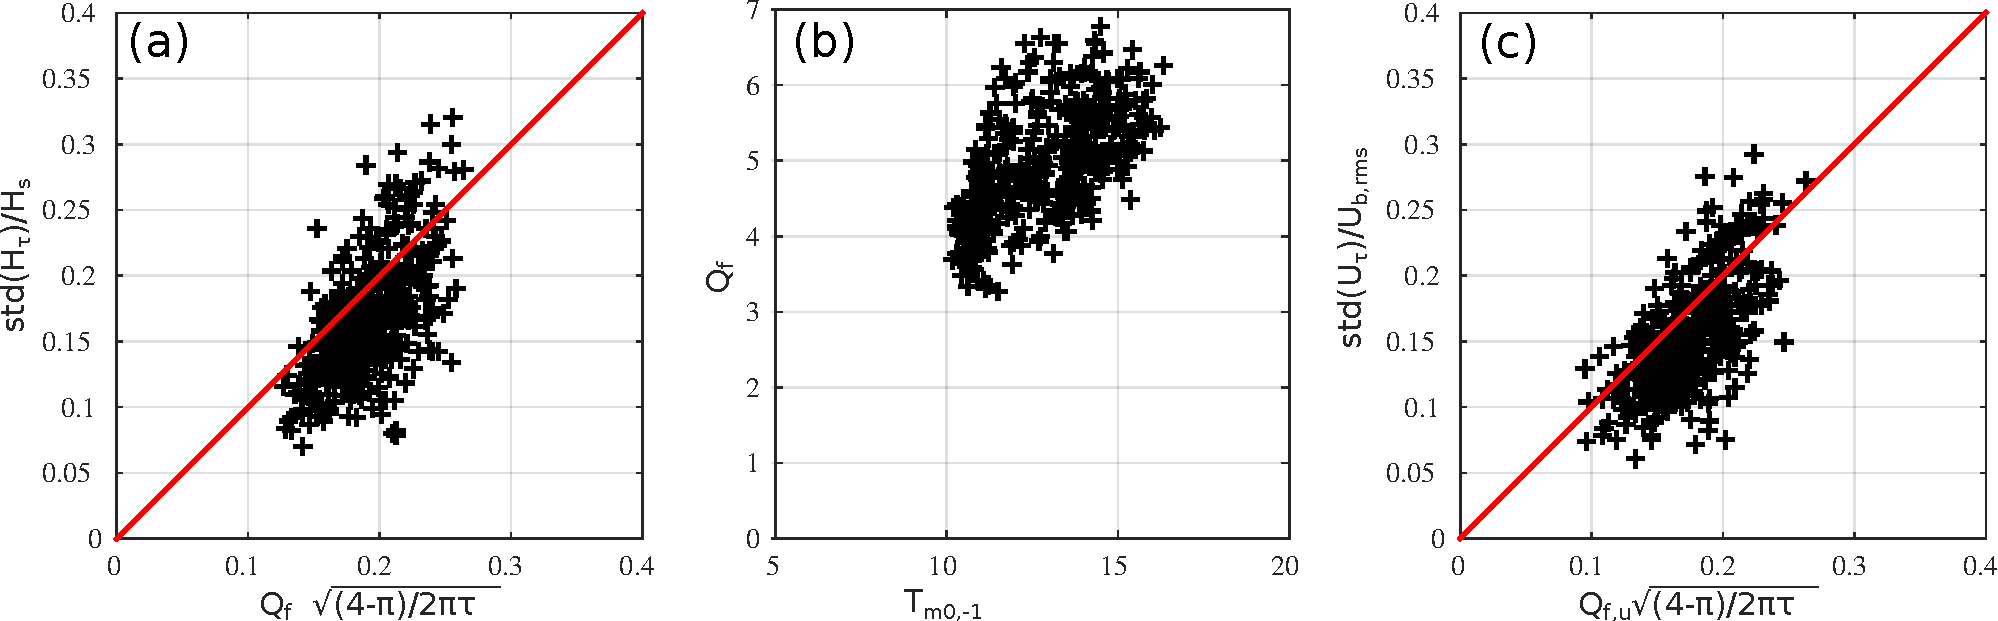
\includegraphics[width=\textwidth]{FIGS_CH_GROUPS/Qf_test.pdf}}
%\vspace{3.64in}
  \caption{Variability of measured parameters over 21 days of measurements in Bertheaume bay, January 2004 using $\tau=180$~s and each symbol corresponds to 1 hour of data: (a) Standard deviation of $H_{\tau}$ normalized by $H_s$ as a function  of the predicted variability using $Q_f$ (b) correlation of $Q_f$ and the mean period $T_{m0,-1}$, (c) variability of bottom orbital velocity amplitude $U_{b,\mathrm{rms}}$ against the relevant $Q_{f,u}$ peakedness parameter.}
\label{fig:groupsQf}
\end{figure}
%%%%%%%%%%%%%%%%%%%%%%%%%%%%%%%%%%%%%%%%%%%%%%%%%%%%%%%
Figure \ref{fig:groupsQf}.a shows that the predicted variability is not exactly like the estimated variability, but it provides a useful order of magnitude, with the "noise" on wave height estimate decreasing like $\sqrt{1/\tau}$, which is why wave records are normally taken over 20 minutes. In the present case, using $2\tau = 20$ minutes averaging instead of averaging over $2\tau = 3$~minutes reduces statistical uncertainties by a factor $\sqrt{20/3}=2.6$, giving a mean value of $\mathrm{std}(H_\tau)/ H_s=6.4\%$, which is of the same order of magnitude as the 5\% relative uncertainty for buoy data for wave heights around 2~m  that is estimated from triple-collocation techniques \citep{Dodet&al.2022}. This suggests that sampling errors caused by wave groups are a large part of the uncertainty in buoy data.

It is always possible to average over longer times but at some point one loses the time resolution that may be needed to investigate how the wave height varies during the tidal cycle or due to other fast evolving phenomena. We also note that quantities that involve higher frequency moments of order $n$ such as the orbital velocity with $n=2$ are less "groupy", their spectrum shape given by $E(f)f^n$ are broader than $E(f)$,  and we can compute a similar $Q_f$ for these parameters that will be lower, as shown in  \ref{fig:groupsQf}.c, using the bottom orbital velocity data from the Nortek Vector instrument. I used pressure and velocity at the ocean bottom in Figure \ref{fig:groupsQf}.a and \ref{fig:groupsQf}.c, and these are already filtered by the water depth, so that the difference between these  $Q_f$  and  $Q_{f,u}$ is not as large as it would be if one used surface elevation and surface velocity.  


\subsection{Spatial maps}
Following the same steps we took for time series, we may imagine that an instrument provides a wave height  $H_{L}$ from a spatial average over a 
square of side $L$ \citep{Lenain&al.2023,Ardhuin&al.2024}. The wave height estimate $H_L$ is  again a $\chi$-distributed random variable with its variance and mean given by  functions of the number of 
degrees of freedom, and their ratio given by eq. (\ref{eq:groups_var_nu}). The only difference is that now  $\nu_{f,H}$ is replaced by 
\begin{equation} 
\nu_{\mathrm{kk},H}=1/ Q_{\mathrm{kk},H}^2 dk_x dk_y \label{eq:nukk}
\end{equation}

 where $dk_x dk_y$ is the spectral resolution of the spectral analysis, corresponding to $dk_x dk_y=(2 \pi)^2/(2 L)^2$, with 
\begin{equation} 
   Q_{\mathrm{kk}}^2 = \frac{  \int_{-\infty}^\infty \int_{-\infty}^\infty E^2(k_x,k_y)\mathrm{d}k_x \mathrm{d}k_y }{\left( \int_{-\infty}^\infty \int_{-\infty}^\infty E(k_x,k_y)\mathrm{d}k_x \mathrm{d}k_y  \right)^2} \label{eq:Qkk},
\end{equation}
where  $E(k_x,k_y)$ is the centrally symmetric double-sided spectrum. If one uses the single-sided spectrum instead, as we did for frequency spectra in eq. (\ref{eq:Qf}), the numerator of eq. (\ref{eq:nukk}) should be 2, as in  eq. (\ref{eq:nuf}). 

This expression is easily verified by taking a wave spectrum $E(k_x,k_y)$, simulating the ocean surface map $\zeta(x,y)$ using random phases, and computing the variance over square tiles of side $L$, as illustrated in Fig. \ref{fig:groups_maps}. The theory, combining eq. (\ref{eq:nukk}) and eq. (\ref{eq:groups_var_nu}) gives 
\begin{equation} 
 \frac{\mathrm{std}(H_L)}{\mathrm{mean}(H_L)} \simeq \pi \sqrt{2}  Q_{\mathrm{kk}} /  L,
   \label{eq:groups_var_2DY}
\end{equation}
which a good approximation in cases where $L$ is much larger than the dominant wavelength. 
%%%%%%%%%%%%%%%%%%%%%%%%%%%%%%%%%%%%%%%%%%%%%%%%%%%%%%%
\begin{figure}[htb]
\centerline{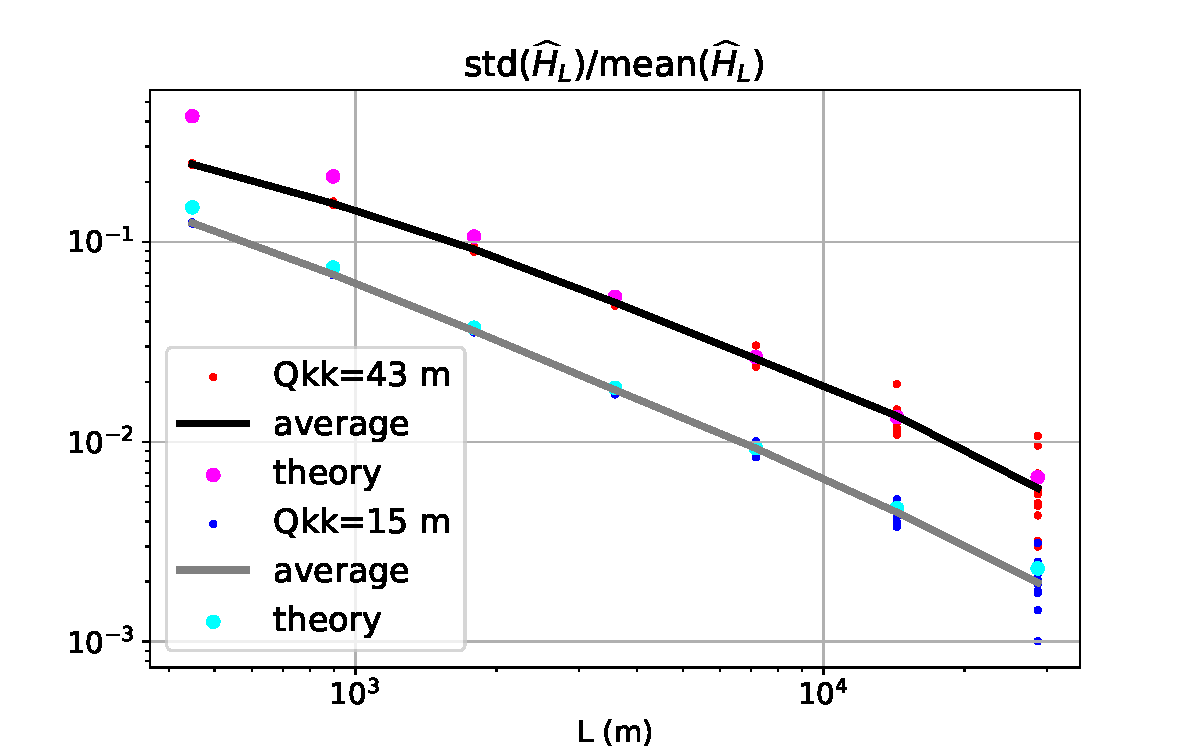
\includegraphics[width=0.9\textwidth]{FIGS_CH_GROUPS/std_maps.pdf}}
%\vspace{3.64in}
  \caption{Variability of $H_L$ in simulated surfaces from 2 different wave spectra, one with $Q_{\mathrm{kk}}=43$~m and the other with $Q_{\mathrm{kk}}=15$~m. These two spectra are shown below in Fig. \ref{figure:groups_storm2}. for each spectrum, 10 surface realisations were generated using random phases, and the average standard deviation is compared to the 
  theoretical value from eq. (\ref{eq:groups_var_2DY}). The notebook that generated this figure is available on \href{https://github.com/ardhuin/waves_in_geosciences/blob/main/NOTEBOOKS/chapter_groups_figure_Qkk_stdH_2D_maps.ipynb}{github}.}
\label{fig:groups_maps}
\end{figure}
%%%%%%%%%%%%%%%%%%%%%%%%%%%%%%%%%%%%%%%%%%%%%%%%%%%%%%%


\subsection{Along-track variability in altimeter data}
A practical important application of the result for spatial maps is the interpretation of the most common measurement of wave heights from space, usinbg satellite altimeters. Looking at data from storm Dennis in the North Atlantic in 2020, as illustrated in Fig. \ref{figure:groups_storm1}, \cite{DeCarlo&al.2023} were surprised to find that for the same mean wave height of 9.3~m, the CFOSAT altimeter beam gave a very small variability on the north side, and a twice larger variability on the south side. What is this variability telling us about the sea state? 
%%%%%%%%%%%%%%%%%%%%%%%%%%%%%%%
\begin{figure}[h!]
\centerline{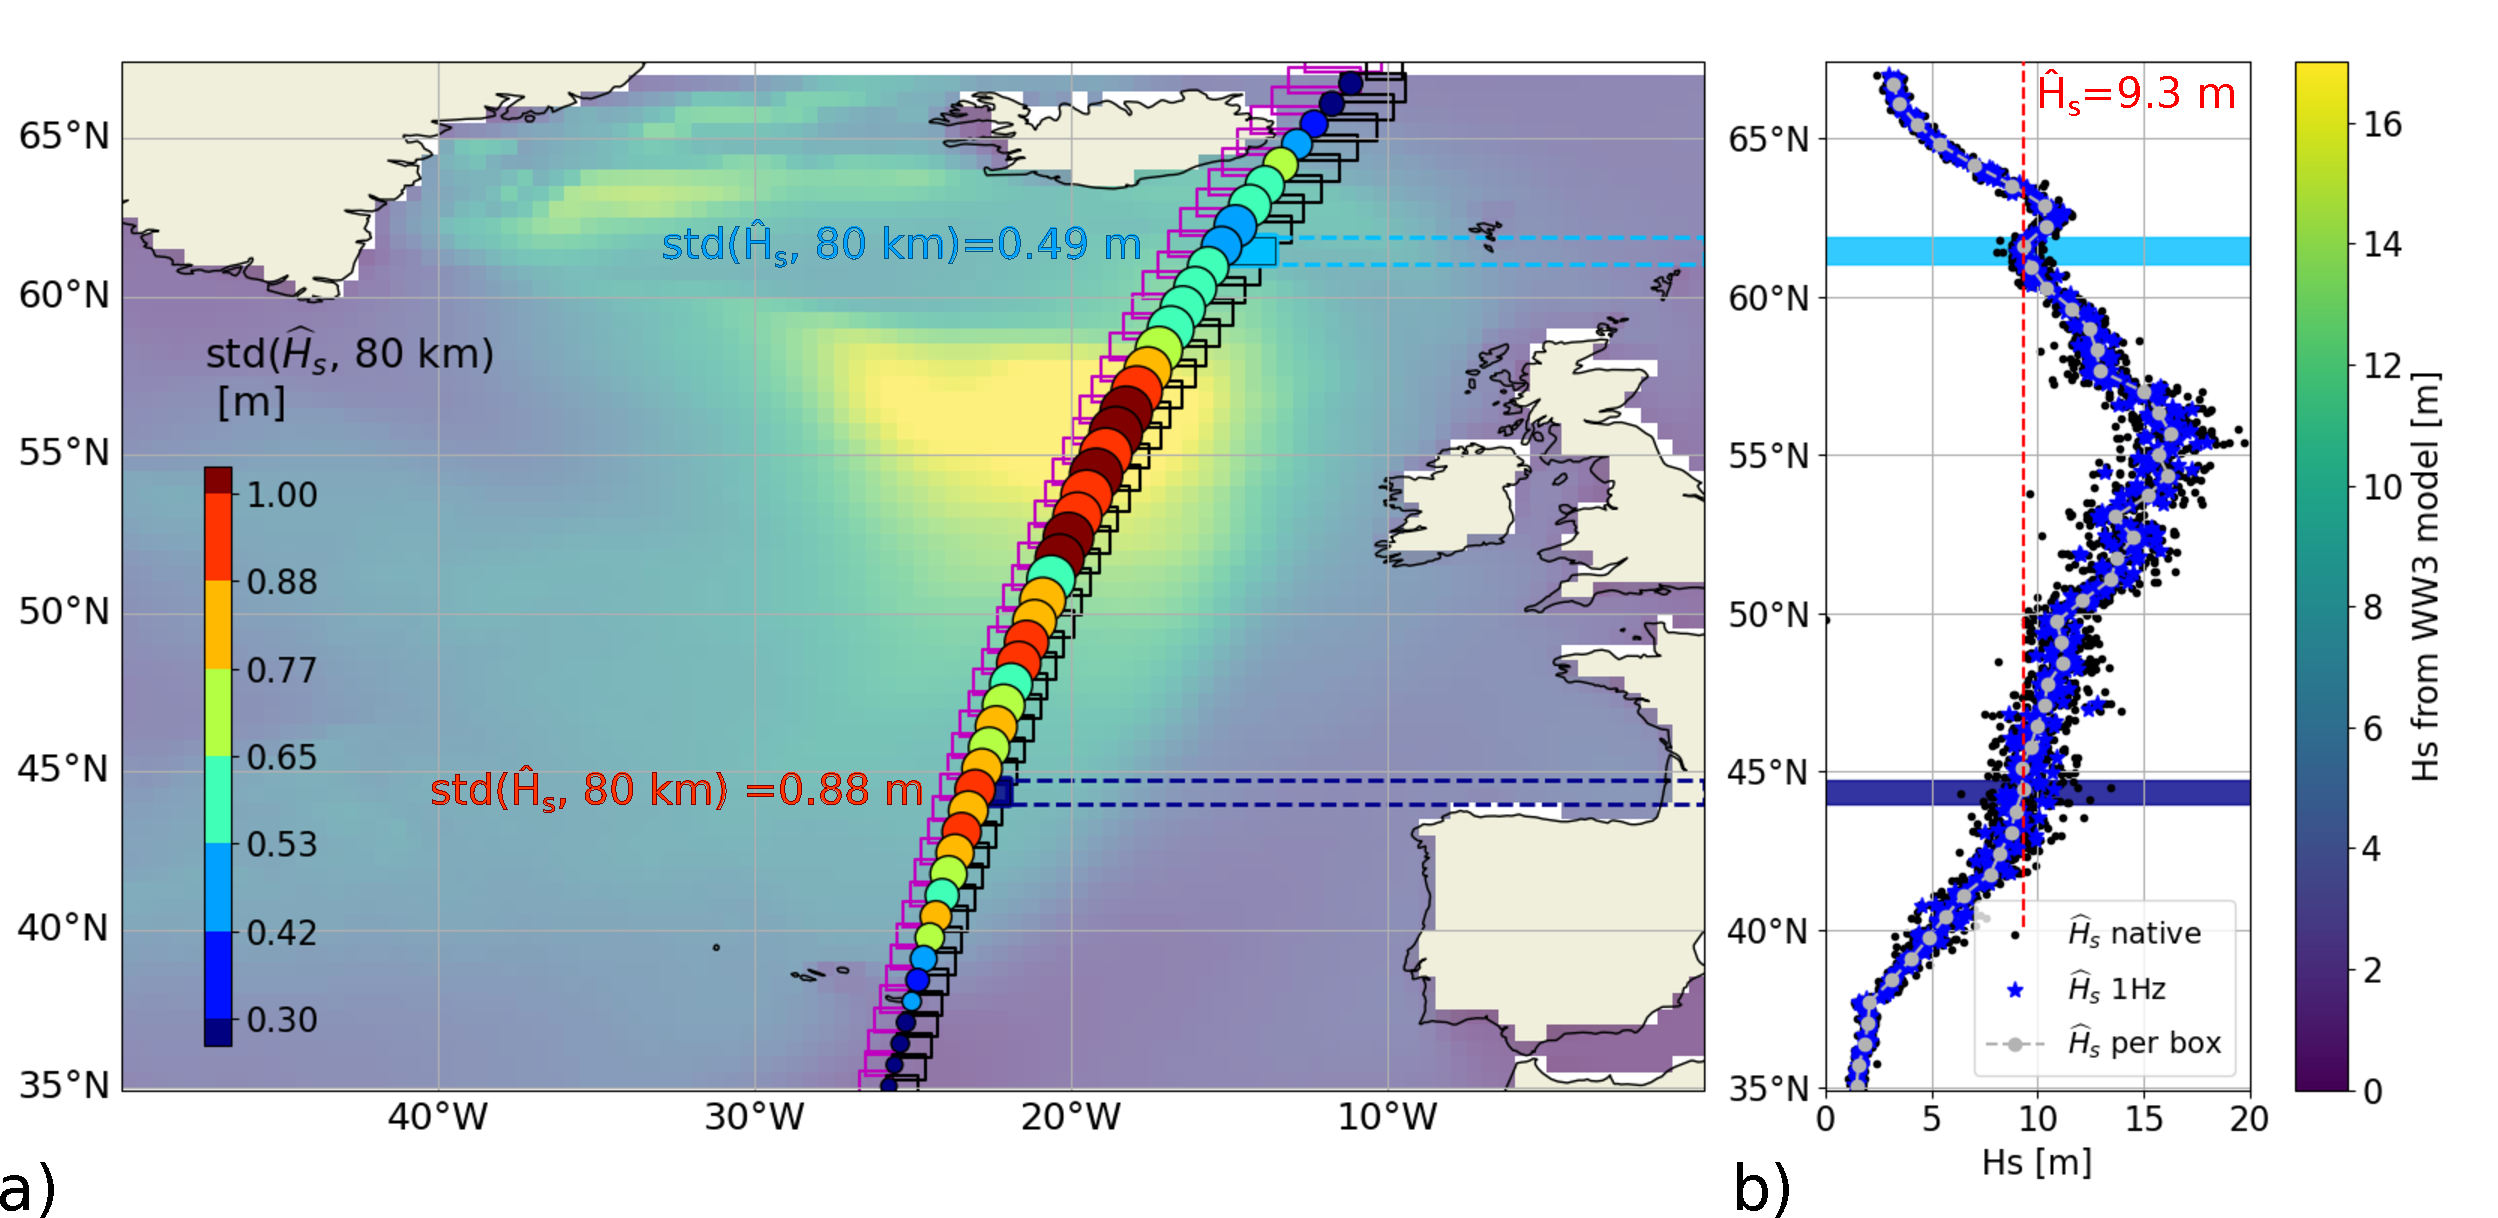
\includegraphics[width=\textwidth]{FIGS_CH_GROUPS/DeCarlo_fig1.pdf}}
    \caption{a) Map of wave heights in the North Atlantic at 09:00 on 14 February 2020, as provided by the model hindcast of \cite{Alday&al.2021}, overlaid with circles located at the center of SWIM box estimates for the L2-CWWIC wave spectra. Circles are sized by the L2-CWWIC $H_s$ estimate and color corresponds to $\mathrm{std}(Hs)$; b) corresponding measured $H_s$ values as a function of latitude (y-axis) : black small dots represent native measurements at 4.5 Hz, blue stars represent the 1~Hz averaged and grey circles represent the $H_s$ averaged over a box. Two boxes are selected for the case study: box A - highlighted in light blue - is at 62$^\circ$N, and box B - in dark blue - is at 44$^\circ$N.} 
   \label{figure:groups_storm1}
\end{figure}
%%%%%%%%%%%%%%%%%%%%%%%%%%%%%%%

The great thing with CFOSAT is that it is the first satellite that combines an altimeter with a wave scatterometer (which provides a measurement of the directional wave spectrum) in the same instrument called SWIM \citep{Hauser&al.2021}. We can thus use the measured wave spectra to understand details in the altimeter data.  In particular we can use the directional spectrum to compute $\Psi$, the spectrum of the envelope. %The maximum value of $H_s$ reported by CFOSAT in the storm was estimated at 17.9~m when using a the average over one measurement cycle (there are 4.5 such measurements per second), or 17.9~m when averaged over 1 s. More interesting to us was, 
Taking the measured wave spectra and simulating the surface and its envelope, as done in Fig. \ref{figure:groups_storm2} makes it easier to visualize the importance of the spectral shape for the defining the spatial variability of wave heights $H_r$. Both panels (c) and (d) correspond to spatially homogeneous sea states with a uniform $H_s$. However, any measurement of waves will be sensitive to the "lumps" of high values and low values that are best seen in the envelope map of Fig. \ref{figure:groups_storm2}.f. The only way to remove this effect of wave groups in the measurements would be to average in time as these groups propagate fast and randomly appear and disappear. 

%%%%%%%%%%%%%%%%%%%%%%%%%%%%%%%
\begin{figure}[hbt!]
\centerline{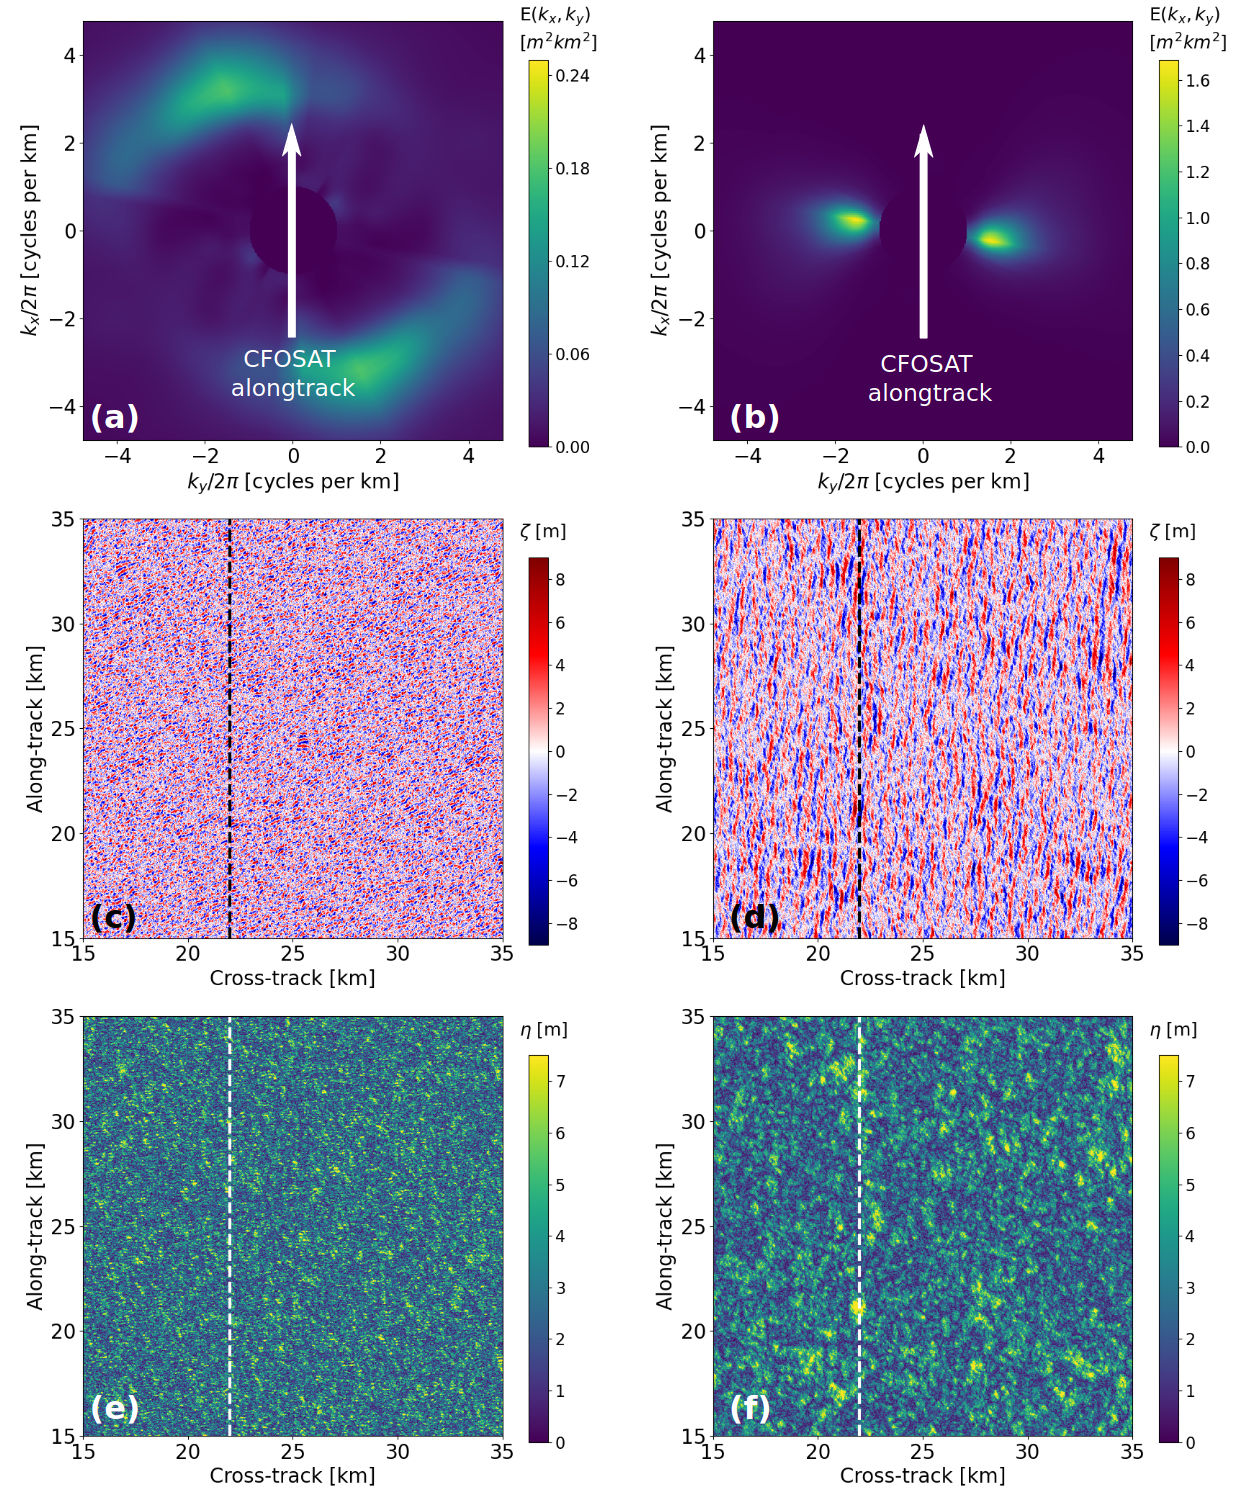
\includegraphics[width=\textwidth]{FIGS_CH_GROUPS/DeCarlo_fig2.jpg}}
    \caption{From wave spectra (top) to surface elevation envelope (bottom): the surface elevations maps in the middle line are simulated using the CFOSAT-derived spectra (these are L2S product corrected to give the same wave height as the nadir beam), with random phases. Combining the real and imaginary parts of the simulated surface gives the envelope. The left column is for a broad wave spectrum with a lower peak period. The right column has the same wave height but a long peak period and narrower spectrum. } 
   \label{figure:groups_storm2}
\end{figure}
%%%%%%%%%%%%%%%%%%%%%%%%%%%%%%%


Although the details will be given only in the next chapter, we may guess that an altimeter samples the ocean with some filtering function that not a square boxcar but some sort of disc of radius $r$, and  we can imagine that the local height is some convolution of the envelope
\begin{equation}
    H_{r}(x,y) = 4\sqrt{\frac{2}{\pi}} (\eta \otimes g_{r})(x,y).
   \label{eq:relation_Hs_eta}
\end{equation}
In practice a single altimeter gives estimates along a single track in the $(x,y)$ plane and the filter function $g_r$ can be a little complicated. For Delay-only altimeters the detailed form of $g_r$ was derived in \cite{DeCarlo&al.2023}, and for our purpose a good approximation is a Gaussian filter of radius $r_a=r_C/4.5$, giving a filter $G_{r_a}=\exp{(-k^2 r_a^2)}$ for the power spectrum in Fourier space, with $r_C$ given by \cite{Chelton&al.1989} as the radius of the region of the ocean surface that may contribute to the measured signal (again, details will follow in the next chapter), 
\begin{equation}
    r_C =\sqrt{\frac{ 2 h_o H_s+ 2 \delta_R}{1+h_o/R_E}} \label{eq:rC}
\end{equation}
where $h_o$ is the satellite orbit height above the ocean, $R_E$ is the Earth radius and $\delta_R$ is the range resolution of the altimeter.  
 
 
Using the double-sided wave spectrum $E(k_x,k_y)$ of the surface elevation, defined for $(k_x,k_y)$ in the entire wavenumber plane and centrally symmetric, the region of the envelope spectrum for $k \ll k_p$, with $k_p$ the wavenumber peak, is 
proportional to
\begin{equation}
    \Psi_{2}(k_x,k_y) = 8 \int_{-\infty}^\infty 
    \int_{-\infty}^\infty
E(u,v)E(u+k_x,v+k_y)\mathrm{d}u \mathrm{d}v,
\end{equation}
in which $\Psi_{2}$ is also double-sided. From  eq.~(\ref{eq:relation_Hs_eta}), the spectrum of $H_r$ is
\begin{eqnarray}
\Psi_{H_r}(k_x,k_y) &= & \frac{32}{\pi}  \Psi(k)  G_{r}(k_x,k_y) =  \underbrace{\frac{32}{\pi} \frac{8 - 2\pi}{H_s^2}   \Psi_2(k_x,k_y)}_{\Psi_{H_0}(k_x,k_y)}  G_{r}(k_x,k_y)\label{eq:eq2_inFourier}
\end{eqnarray}
with $H_s$ the usual significant wave height and $G_{r}=G_{r_a}$ when considering a single altimeter measurement.

We will now average data along the track, at least over 0.05~s corresponding to the 20~Hz rawest data downlinked for most instruments, and corresponding to 350~m distance along the track. For delay-only measurements, these data are fairly noisy and most users typically use at least 1~Hz data (averaged over 7~km) or longer time averages. For simplicity we take the satellite track along the $x$-axis, and we consider an averaging length $d_1$. 
Integrating $\Psi$ for $k_x > k_1$, amounts to integrating $\Psi_{H_r}(k_x,k_y)$ to get the expected variance up to the  cut-off wavenumber along $k_x$, $k_1\simeq \pi / d_1 $, giving $\mathrm{var}(H_{r},d_1)$, the group-induced fluctuations of $\widehat{H}_s$ 
\begin{equation}
\mathrm{var}(H_{r}, d_1) = \int_{-\infty}^{\infty} \int_{k_x > |k_1| } \Psi_{H_0}(k_x,k_y)  G_{r}(k_x,k_y) \mathrm{d}k_x \mathrm{d}k_y. \label{eq:varfromspec2D}
\end{equation}
% pi/2 * (2/ra^2 - 4 k1 / sqrt(pi) ra) = pi * ka^2 - 2 ka*2k1  ka = 
Here again, if the filter $G_{r}$ is zero outside of a very small range of wavenumbers, we can approximate $\Psi_{H_0}(k_x,k_y) \simeq \Psi_{H_0}(k_x=0,k_y=0)$ and take this value out of the integral, and the integral is related to the effective area of the filter in the wavenumber plane which we approximate as a disk of radius $1/r_a$, with an area $\pi /r_a^2$, given by the integral of $G_{r}$ over the entire wavenumber plane, and we remove a band of width $2 k_1$ and length $2/r_a$ because we are only averaging over $d_1$ so that wavelengths longer than $2 d_1$ cannot contribute to our signal and must be excluded. This gives,  
\begin{eqnarray}
    \mathrm{var}(H_{r},d_1) &\simeq&  \Psi_{H_0}(0,0)   \int_{-\infty}^{\infty} \int_{k_x > |k_1| } G_{r}(k_x,k_y) \mathrm{d}k_x \mathrm{d}k_y \nonumber \\
    &\simeq&  \Psi_{H_0}(0,0)  \pi\left(1 / {r_a}^2 - 4 k_1/ r_a \right) \nonumber\\
    &\simeq&  \frac{32}{\pi} \frac{8 - 2\pi}{H_s^2}   \Psi_2(0,0)   \pi  \left(1 / {r_a}^2 - 4 k_1/ r_a \right) \nonumber\\
    &\simeq&   Q_{kk}^2 H_s^2(8 - 2 \pi) \left(1 / {r_a}^2 - 4 k_1/ r_a \right)  , 
\end{eqnarray}
where we have defined 
a two-dimensional spectral peakedness $Q_{kk}$ which is measured in meters,
\begin{equation}
    Q_{kk}^2 = \frac{\iint_{} E^2(k_x,k_y)\mathrm{d}k_x\mathrm{d}k_y}{\left(\iint_{}E(k_x,k_y) \mathrm{d}k_x\mathrm{d}k_y\right)^2} = \frac{32 \Psi_2(k_x=0,k_y=0)}{H_s^4}.
\label{eq:bandwith_2D}
\end{equation}


This expression gives the approximate value for the standard deviation,
\begin{equation}
    \mathrm{std}(H_{r},d_1) \simeq  H_s   Q_{kk}  \sqrt{ (4-\pi) \left[2/r_a^2 -  8 k_1 / r_a\right] }.\label{eq:std_Hs_from_Qkk}
\end{equation}

{This variability of $H_{r_a}$, which we have defined as the contribution of wave groups to the variability of "measured" wave heights $\widehat{H}_s$ is thus the product of three factors: the significant wave height $H_s$, the shape of the wave spectrum as quantified by $Q_{kk}$, and the effective range of spatial scales over which the variance is integrated. That last factor is a function of the smoothing effect of the altimeter, represented by the filtering scale $r_a$, and the distance $d_1=2\pi / k_1$ over which  we consider the variability.


%%%%%%%%%%%%%%%%%%%%%%%%%%%%%%%
\begin{figure}[ht!]
\centerline{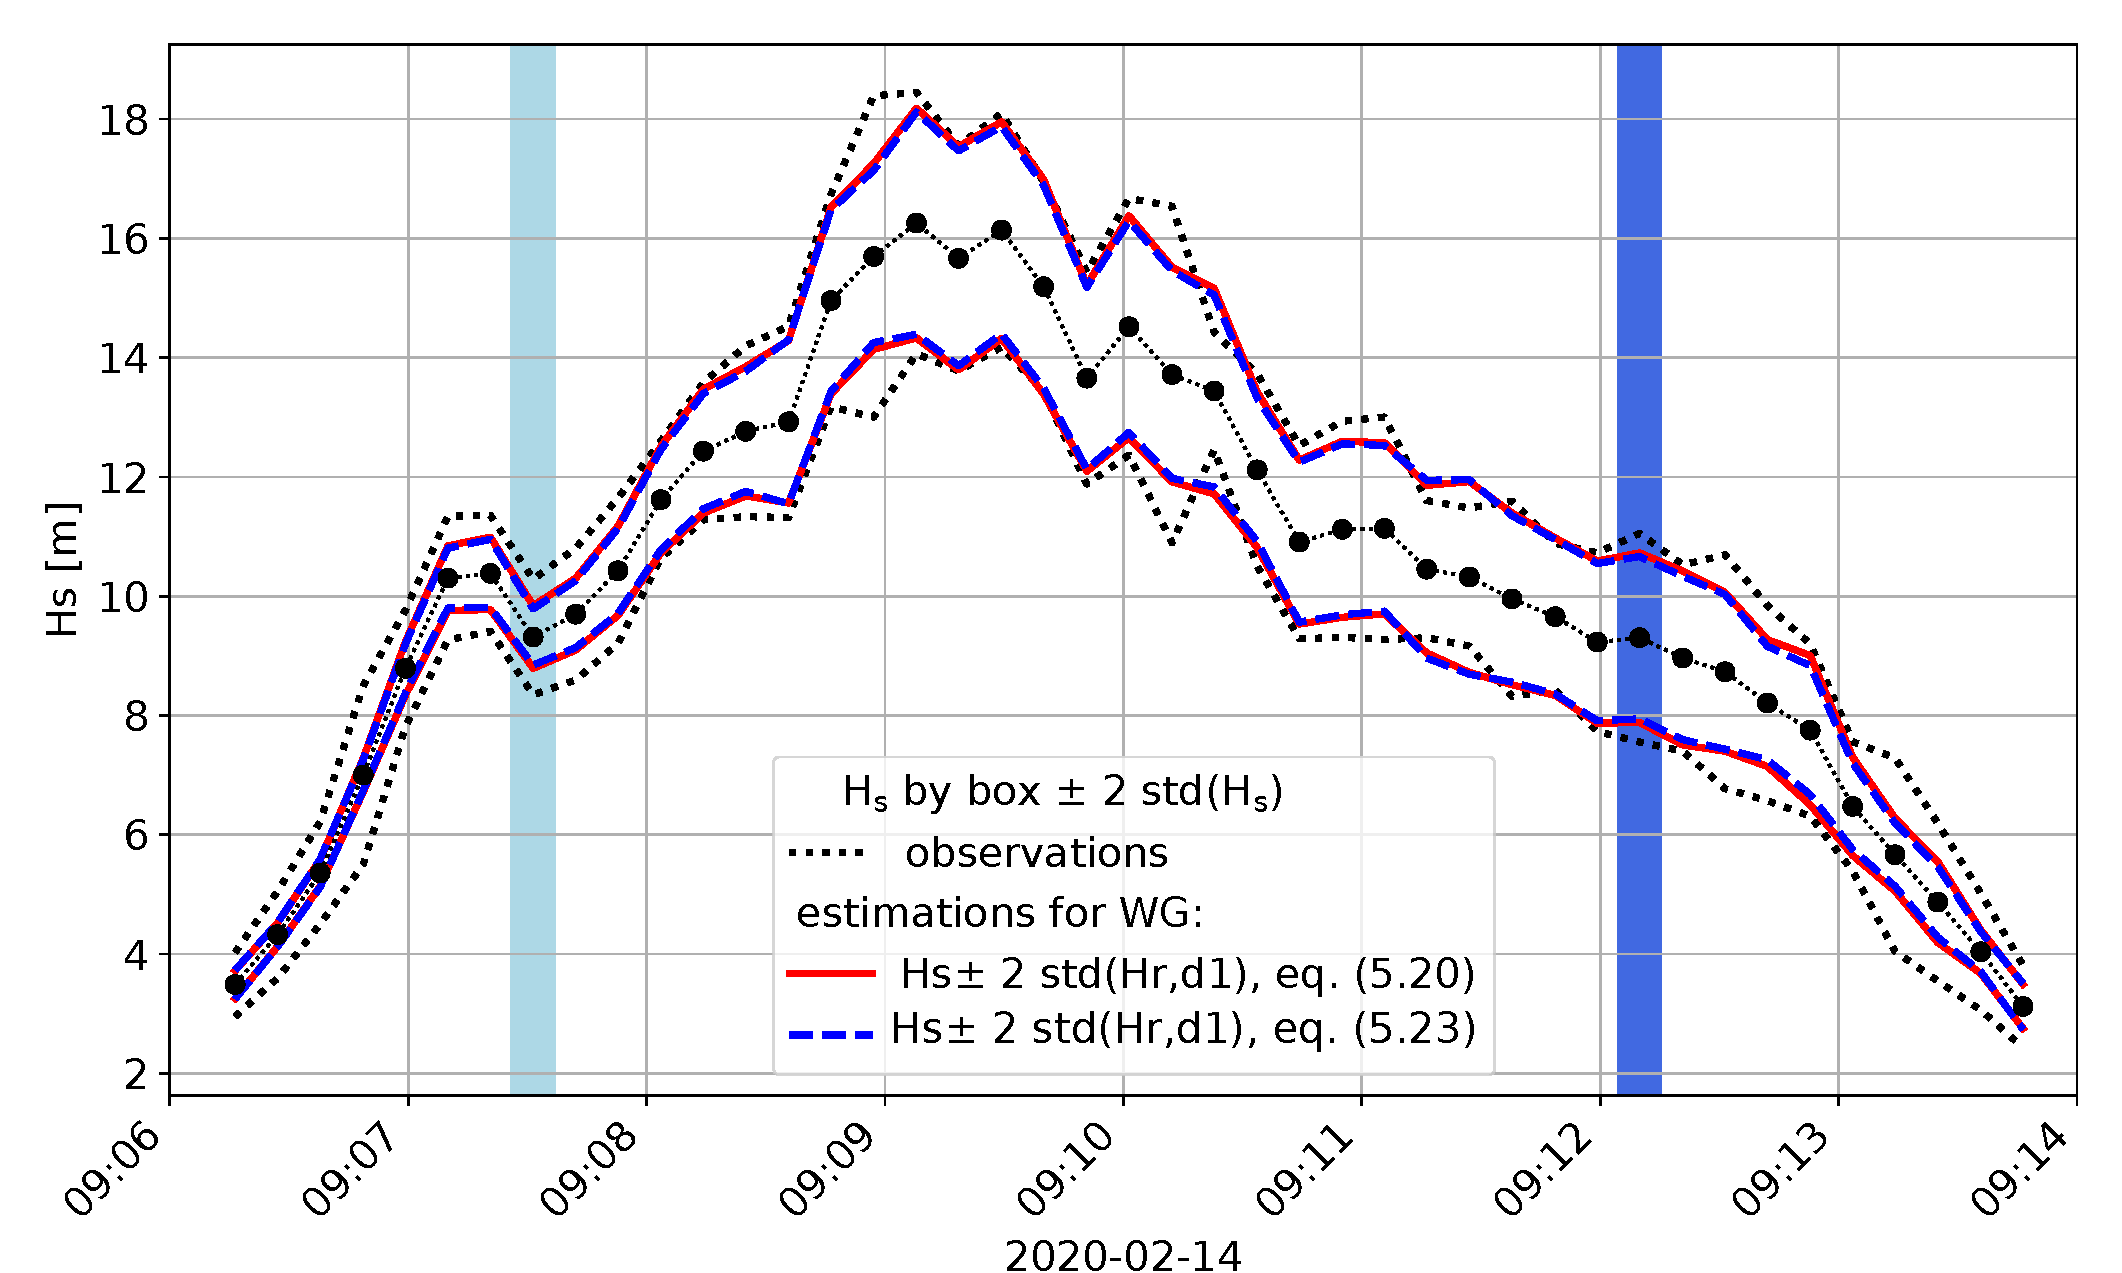
\includegraphics[width=0.75\textwidth]{FIGS_CH_GROUPS/groups_Storm_Dennis_2023_fig3.pdf}}
    \caption{Values of measured $H_s$, averaged over 80~km - black circles - ,  and corresponding $\mathrm{std}(Hs)$ - black dash-dotted lines - in the satellite data, for the CFOSAT track shown in Fig.~\ref{figure:groups_storm1}. Estimations of $\mathrm{std}(H_r,d_1)$ are also represented - in red and blue.} 
   \label{figure:groups_storm3}
\end{figure}
%%%%%%%%%%%%%%%%%%%%%%%%%%%%%%%
We can use our theory to verify that in the case of narrow spectra, the expected effect of wave groups gives a standard deviatin of the estimates of wave heights $H_r$ that is similar to the standard deviation of the measurement over a 80~km segment along the satellite track (Fig. \ref{figure:groups_storm3}). 

On the contrary, for the broader wave spectrum, the effect of wave groups is much smaller than in the measurements: it is possible that the data contains true gradients of the underlying $H_s$, and we also know that measurement noise (known as speckle) is often the dominant source of variability in the measured values. This is one of the main reason for the development of Delay-Doppler altimetry which has a much lower level of speckle noise due to the averaging of different indepedent Doppler "looks" for the same measurement. 

Using eq. (\ref{eq:std_Hs_from_Qkk}) we can remove the expected contribution of groups and study the influence on other factors on the variability of $H_s$. Figure \ref{fig:groups_global1}, shows that the relative fluctuations in significant wave height is clearly associated with regions of strong mesoscale currents, as we will see in chapter \ref{ch_current}. However, in order to be able to transpose these results to other satellites, we now have to go back to these assumptions about how altimeters actually work, and do a little bit of theory about these instruments and what they actually measure: nadir altimeter do not measure wave height or sea level, they measure waveforms from which wave height and sea level are estimated. 


%%%%%%%%%%%%%%%%%%%%%%%%%%%%%%%
\begin{figure} [ht!]
   \centerline{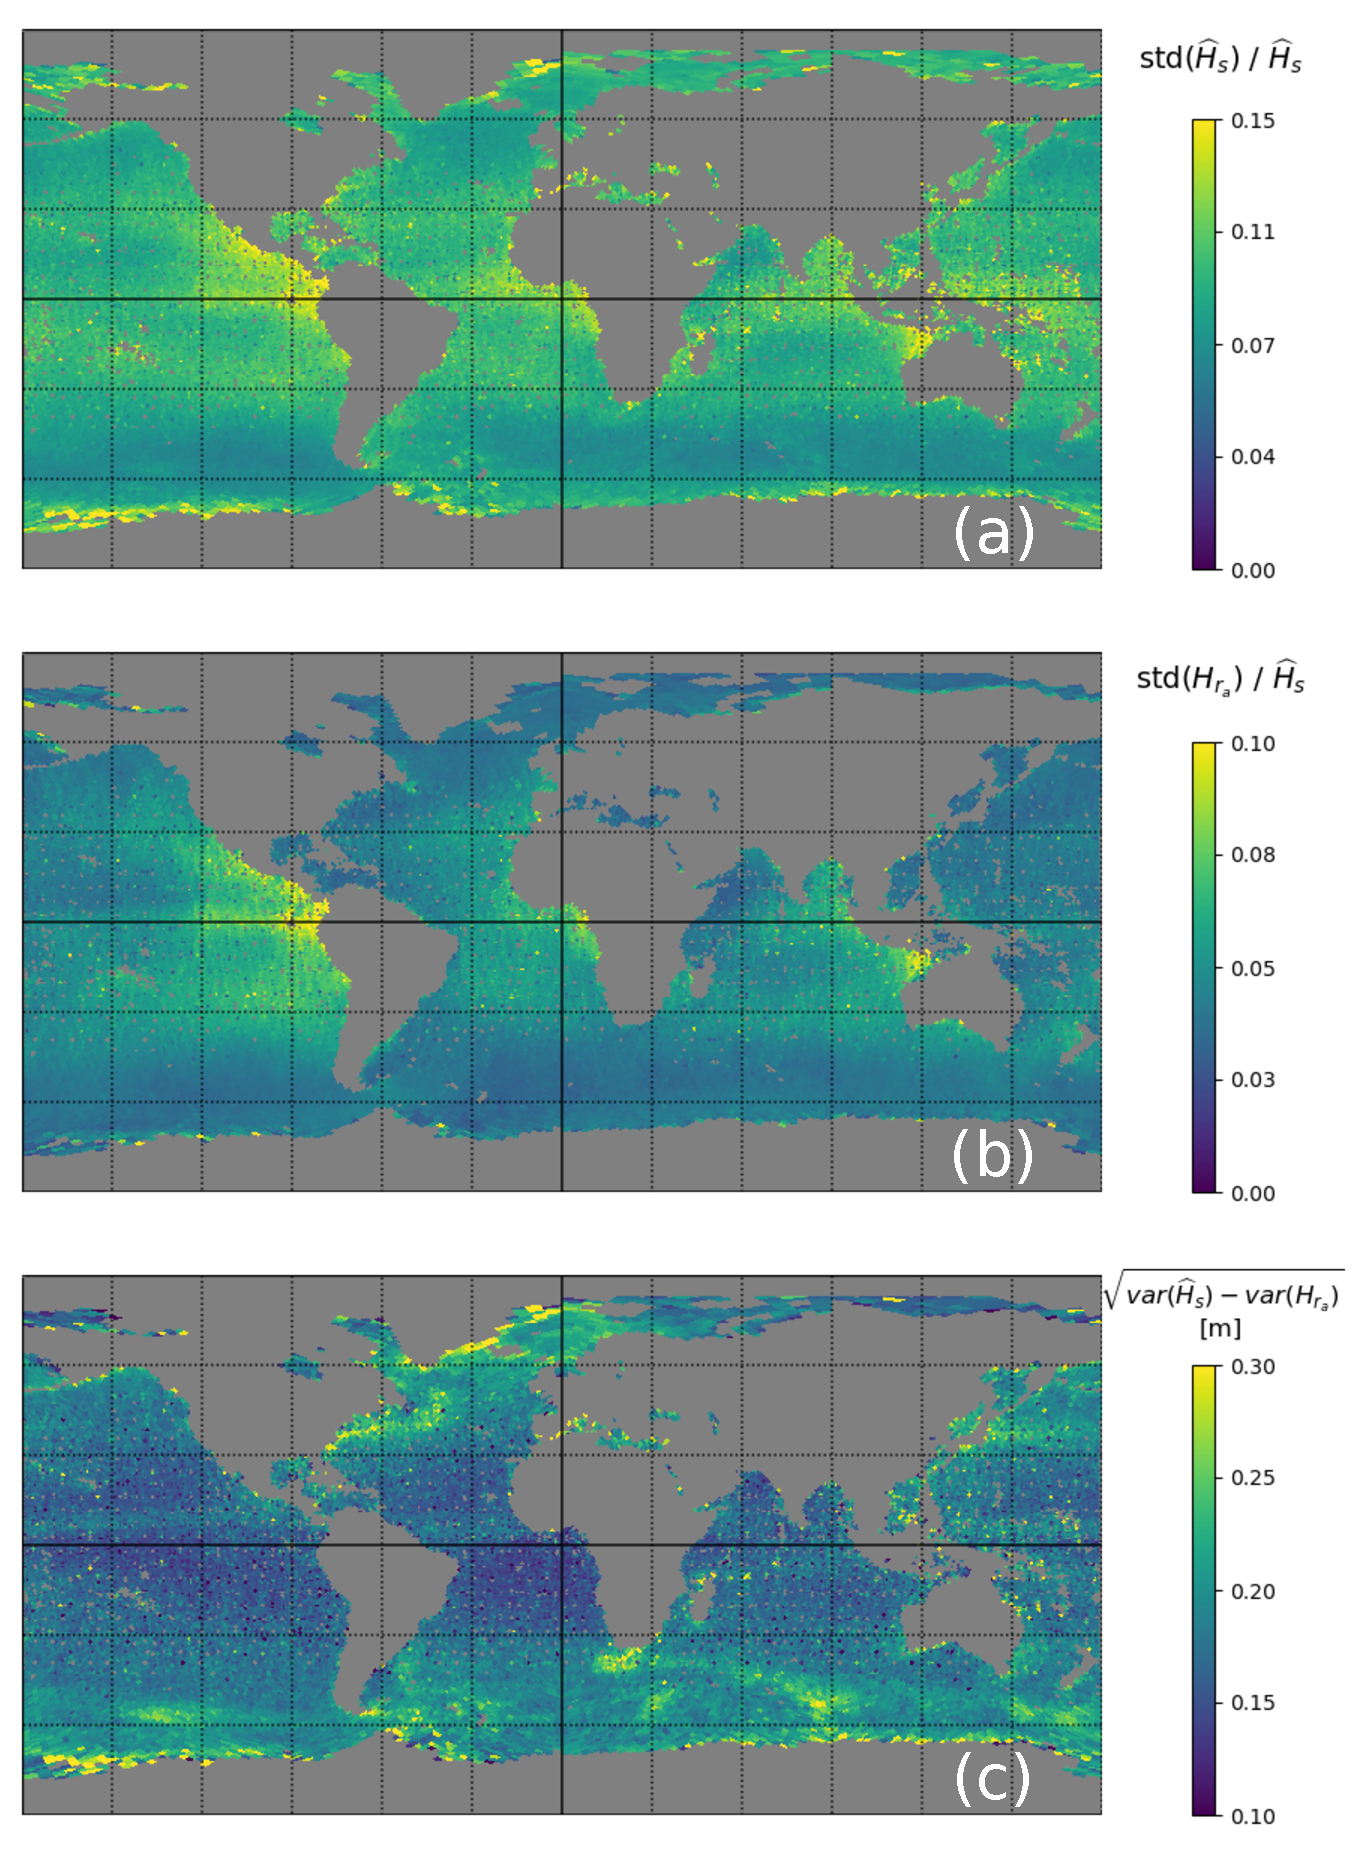
\includegraphics[width=\linewidth]{FIGS_CH_GROUPS/Fig8_map_stdHs_byHs_nadir_vs_L2S.pdf}}
    \caption{Map of the average of a) $\mathrm{std}(\widehat{H}_s)/\mathrm{mean}(\widehat{H}_s)$ - upper panel -, b) $\mathrm{std}(H_s)_\mathrm{{wg}}/\mathrm{mean}(H_s)$ -middle panel - and c) residual standard deviation of $H_s$, in meters, after removing the effect expected
from wave groups - lower panel -, for the years 2020 and 2021 for all the SWIM L2-IWWOC boxes with a $H_s$ above 1.5 m. With the wave group contribution $\mathrm{std}(H_s)_\mathrm{{wg}}$ estimated from SWIM L2S spectra.  reproduced from \cite{DeCarlo&al.2023}.} 
   \label{fig:groups_global1}
\end{figure}
%%%%%%%%%%%%%%%%%%%%%%%%%%%%%%%



\cleardoublepage
\chapter{Wave data from satellites: Skylab (1975) to SWOT (2025)}\label{ch_sat}

It is not possible to cover in a single chapter all the technical development in radar instruments and their processing over the last 50 years. We will thus focus mostly on nadir radar altimeters with some discussion of complementary measurements from Synthetic Aperture Radar (SAR) and wave spectrometer systems. Hopefully more chapters will pop up in Part 3 to go beyond 
this presentation. 

\section{General considerations about radar remote sensing}
Since the invention of radar, the sea was found to be an important source of echoes, at all radar frequencies (from decametric to micro waves). 
This is due to the dielectric properties of sea water. An active radar measures the electromagnetic power received by its antenna. Using the radar equation, this power (in Watts)
is normalized by the antenna-target distance, the antenna size, and the emitted power. This gives the normalized radar cross section (NRCS), a quantity without dimensions that is often represented 
by the symbol $\sigma_0$. 
$\sigma_0$ depends on the surface geometry but it also varies with the radar frequency and polarization,  and observation direction (azimuth and incidence angles). %In particular, $\sigma_0$ highly depends on the radar wavelength and of the wave radar incidence angle relative to the surface.
The phase properties of the signal can also be used to estimate velocities at the ocean surface: current and wave orbital velocities \citep{Nouguier&al.2018,Rodriguez2018}. 

%A down-looking (nadir) radar will measure a high $\sigma_0$ for a smooth sea surface. If waves are present, the surface echoes may be considered as the incoherent superposition of the facet echoes. 
%%%%%%%%%%%%% figure
\begin{figure}[htb]
\centerline{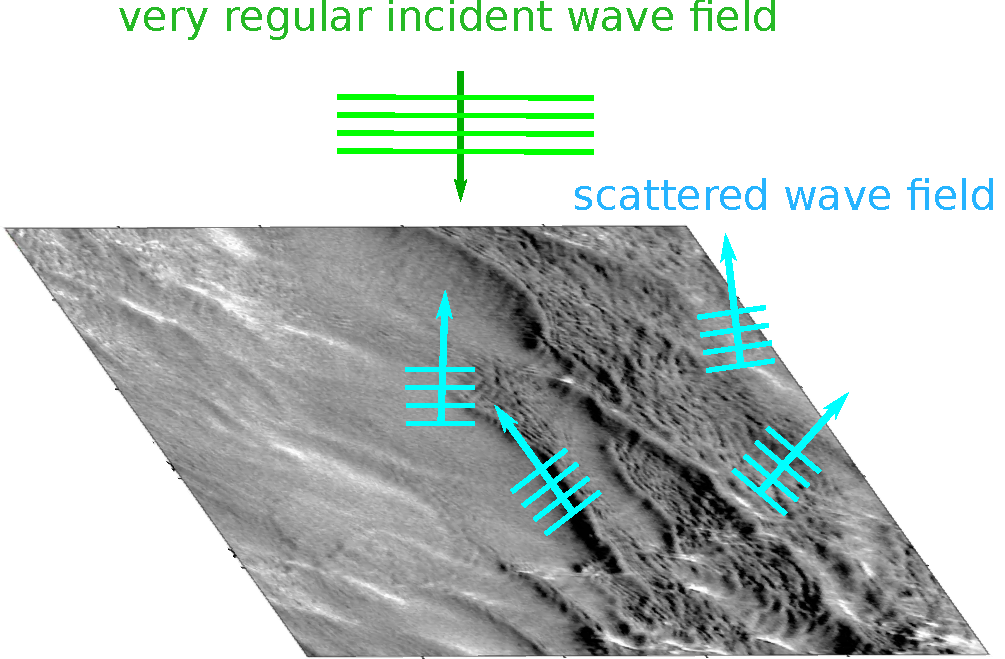
\includegraphics[width=0.7\textwidth]{FIGS_CH_SAT/scatter.pdf}}
%\vspace{3.64in}
  \caption{Conceptual schematic of microwave radar waves scattering at the sea surface. The grey shades are an example of a map of surface slopes estimated from a polarimetric system and covering a region of about 1 by 1 meter \citep{Laxague&al.2018}.}\label{fig:scatter}
\end{figure}
%%%%%%%%%%%%% end of figure
Now, before we look at radar power of phase, one should realize a few important facts 
\begin{itemize}
\item within the radar field of view, the echoes recieved by the radar are coming from only a very small fraction of the surface: where the ocean is smooth (at the scale of the radar wavelength) only those pieces of the ocean surface that are facing the radar will contribute to the measured reflected signal, where the surface is curved, there will be a very weak scattering in all directions. 
\item the many sources of the echoes on the sea surface have randomly distributed distances (and velocities) relative to the radar, so that  the relative phase of all the echoes is randomly distributed and the sum of the electric fields from all these random sources will have highly fluctuating amplitudes within a few milliseconds as the ocean surface moves: this effect is called "Rayleigh fading" and it introduces speckle noise in the radar measurements. This is very similar to the presence of wave groups in narrow-banded wave spectra. 
\end{itemize}


%\subsection{Satellite radar altimeters}
The choice of the radar frequency is dictated by 
a number of considerations, including atmospheric absorption -- we want to be able to measure a returning echo from the sea surface -- and the 
size of the antenna -- low frequencies give large wavelength that require a proportionally large antenna to have a narrow beam. The radar wavelength 
and frequency are related by the speed of light $c$, namely $f_r = c / \lambda_r$. Different frequency bands have been reserved for Earth remote sensing, although they can be contaminated by military radars and other 
systems. Note that telecommunication systems (FM radio, TV channels, GSM networks, GPS/Galileo positionning systems ...) use different bands  also in the microwave range, and remote sensing may use these 
sources of opportunity for signals that reflect off the sea surface  \citep[e.g.][]{Lowe&al.2002}.


%%%%%%%%%%%%%%%%%%%%%%%%%%%%%%%%%%%%%%%%%%%%%%%%%%%%%%%%%%%%%%%%%%%%%%%%%%%%
\begin{table}[hb]
  \centering
  \begin{tabular}{|c|c|c|c| c |}
 \hline
band name & frequency & wavelenghth & example instrument & satellite  carrying the instrument  \\
 \hline
W  & 94 GHz  & 0.3 cm & CPR & Cloudsat  \\
Ka & 30 GHz  & 0.8 cm & AltiKa or KaRIN & SARAL or SWOT  \\
Ku & 15 GHz  & 2.2 cm & Poseidon 3 & Jason 3  \\
X &  9.6 GHz & 3.1 cm & & TerraSAR-X  \\
C & 6 GHz   & 5 cm & Poseidon 3 or ASCAT & Jason 3 or MetOp \\
S & 3 GHz   & 12 cm & S-SAR &  NISAR \\
L & 1.5 GHz  & 24 cm & SMAP  & SMAP \\
P & 435 MHz  & 70 cm & P-SAR & Biomass (launch  in 2024 or 2025) \\
\hline
\end{tabular}
\caption{Typical average frequencies and wavelengths used for ocean remote sensing in the different radar microwave bands. The actual frequency usually varies during a radar pulse with a bandwidth $B$ that defines 
the range resolution of the instrument. \label{table_radars}}
\label{table_bands}
\end{table}
%%%%%%%%%%%%%%%%%%%%%%%%%%%%%%%%%%%%%%%%%%%%%%%%%%%%%%%%%%%%%%%%%%%%%%%%%%%%

Ocean waves have been monitored from space continuously since the lauch of ERS-1 using altimeters and SARs, as summarized in figure \ref{fig:satellite}
%%%%%%%%%%%%% figure
\begin{figure}[htb]
\centerline{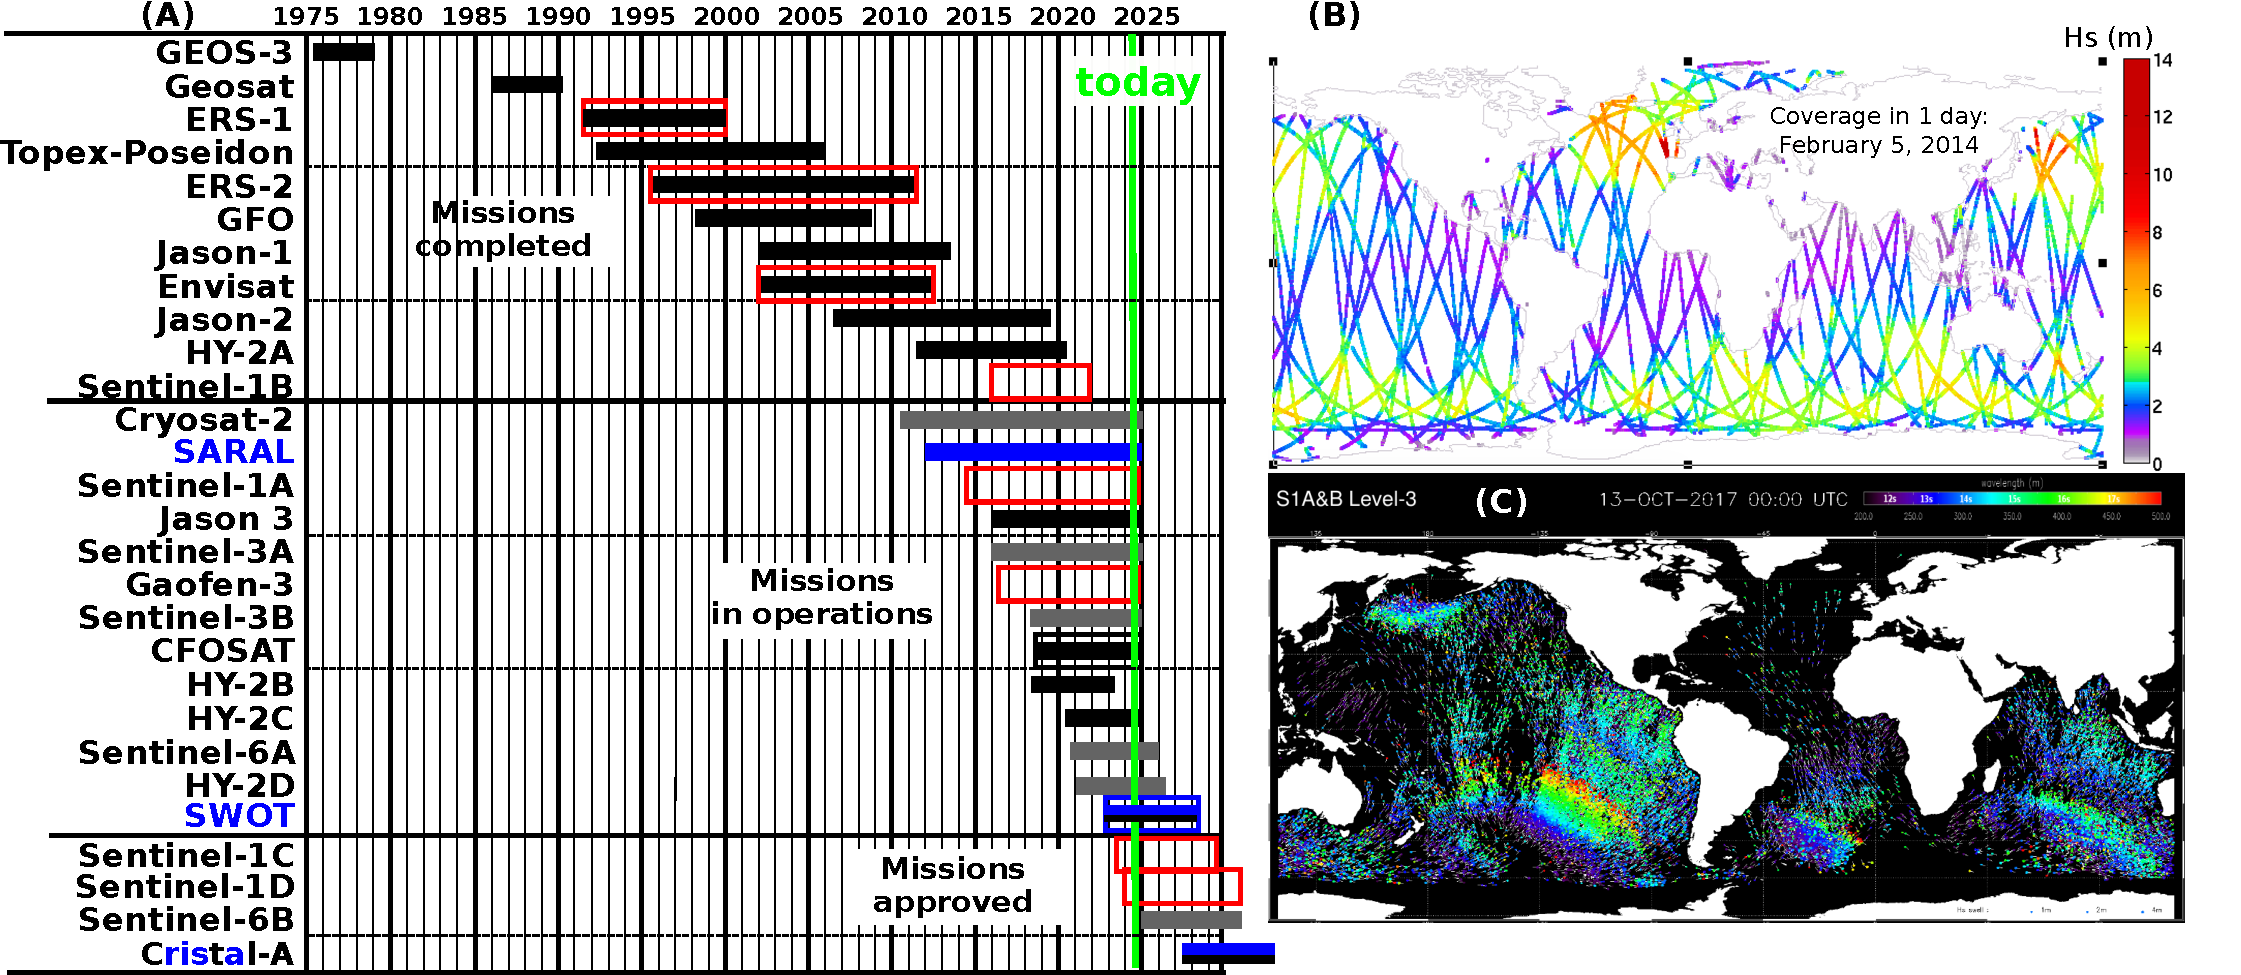
\includegraphics[width=\textwidth]{FIGS_CH_SAT/missions.pdf}}
%\vspace{3.64in}
  \caption{Satellite missions with sea state monitoring objectives.}
    {Time coverage of satellite missions from 1985 to 2030, including nadir and near-nadir altimeters (solid bars), and missions monitoring ocean wave spectra (open boxes) using C-band Synthetic Aperture Radars (red), and real aperture radars in Ku-band (black) or Ka-band (blue). The lighter color (grey and blue) bars correspond to altimeters using Delay-Doppler processing. Source: CEOS database
    \url{http://database.eohandbook.com/}). (B) example of 1-day coverage for Hs measurements with 4 satellite altimeters 
    (C) snapshot of a 'fireworks' plot, the showing the height (size of symbols) peak periods (colors), and directions (barbs) of 
    swell partitions derived from Sentinel-1A and Sentinel-1B wave mode data. Such plots are produced routinely by CMEMS.}\label{fig:satellite}
\end{figure}
%%%%%%%%%%%%% end of figure

\section{Radar altimeters and the The Brown-Hayes model: echoes from a spatially uniform ocean}
Radar altimeter data are, the source of measurements of $H_s$  available at global scale and used for operational wave forecasting
through data assimilation. Contrary to other observation systems, $H_s$ is directly estimated, without the use of a spectral analysis. The usual 
arrangement is a radar antenna looking straight down - at the nadir - on the the sea surface. 

\subsection{Conventional or `delay' altimetry}\label{delay}
%%%%%%%%%%%%% figure
\begin{figure}[htb]
\centerline{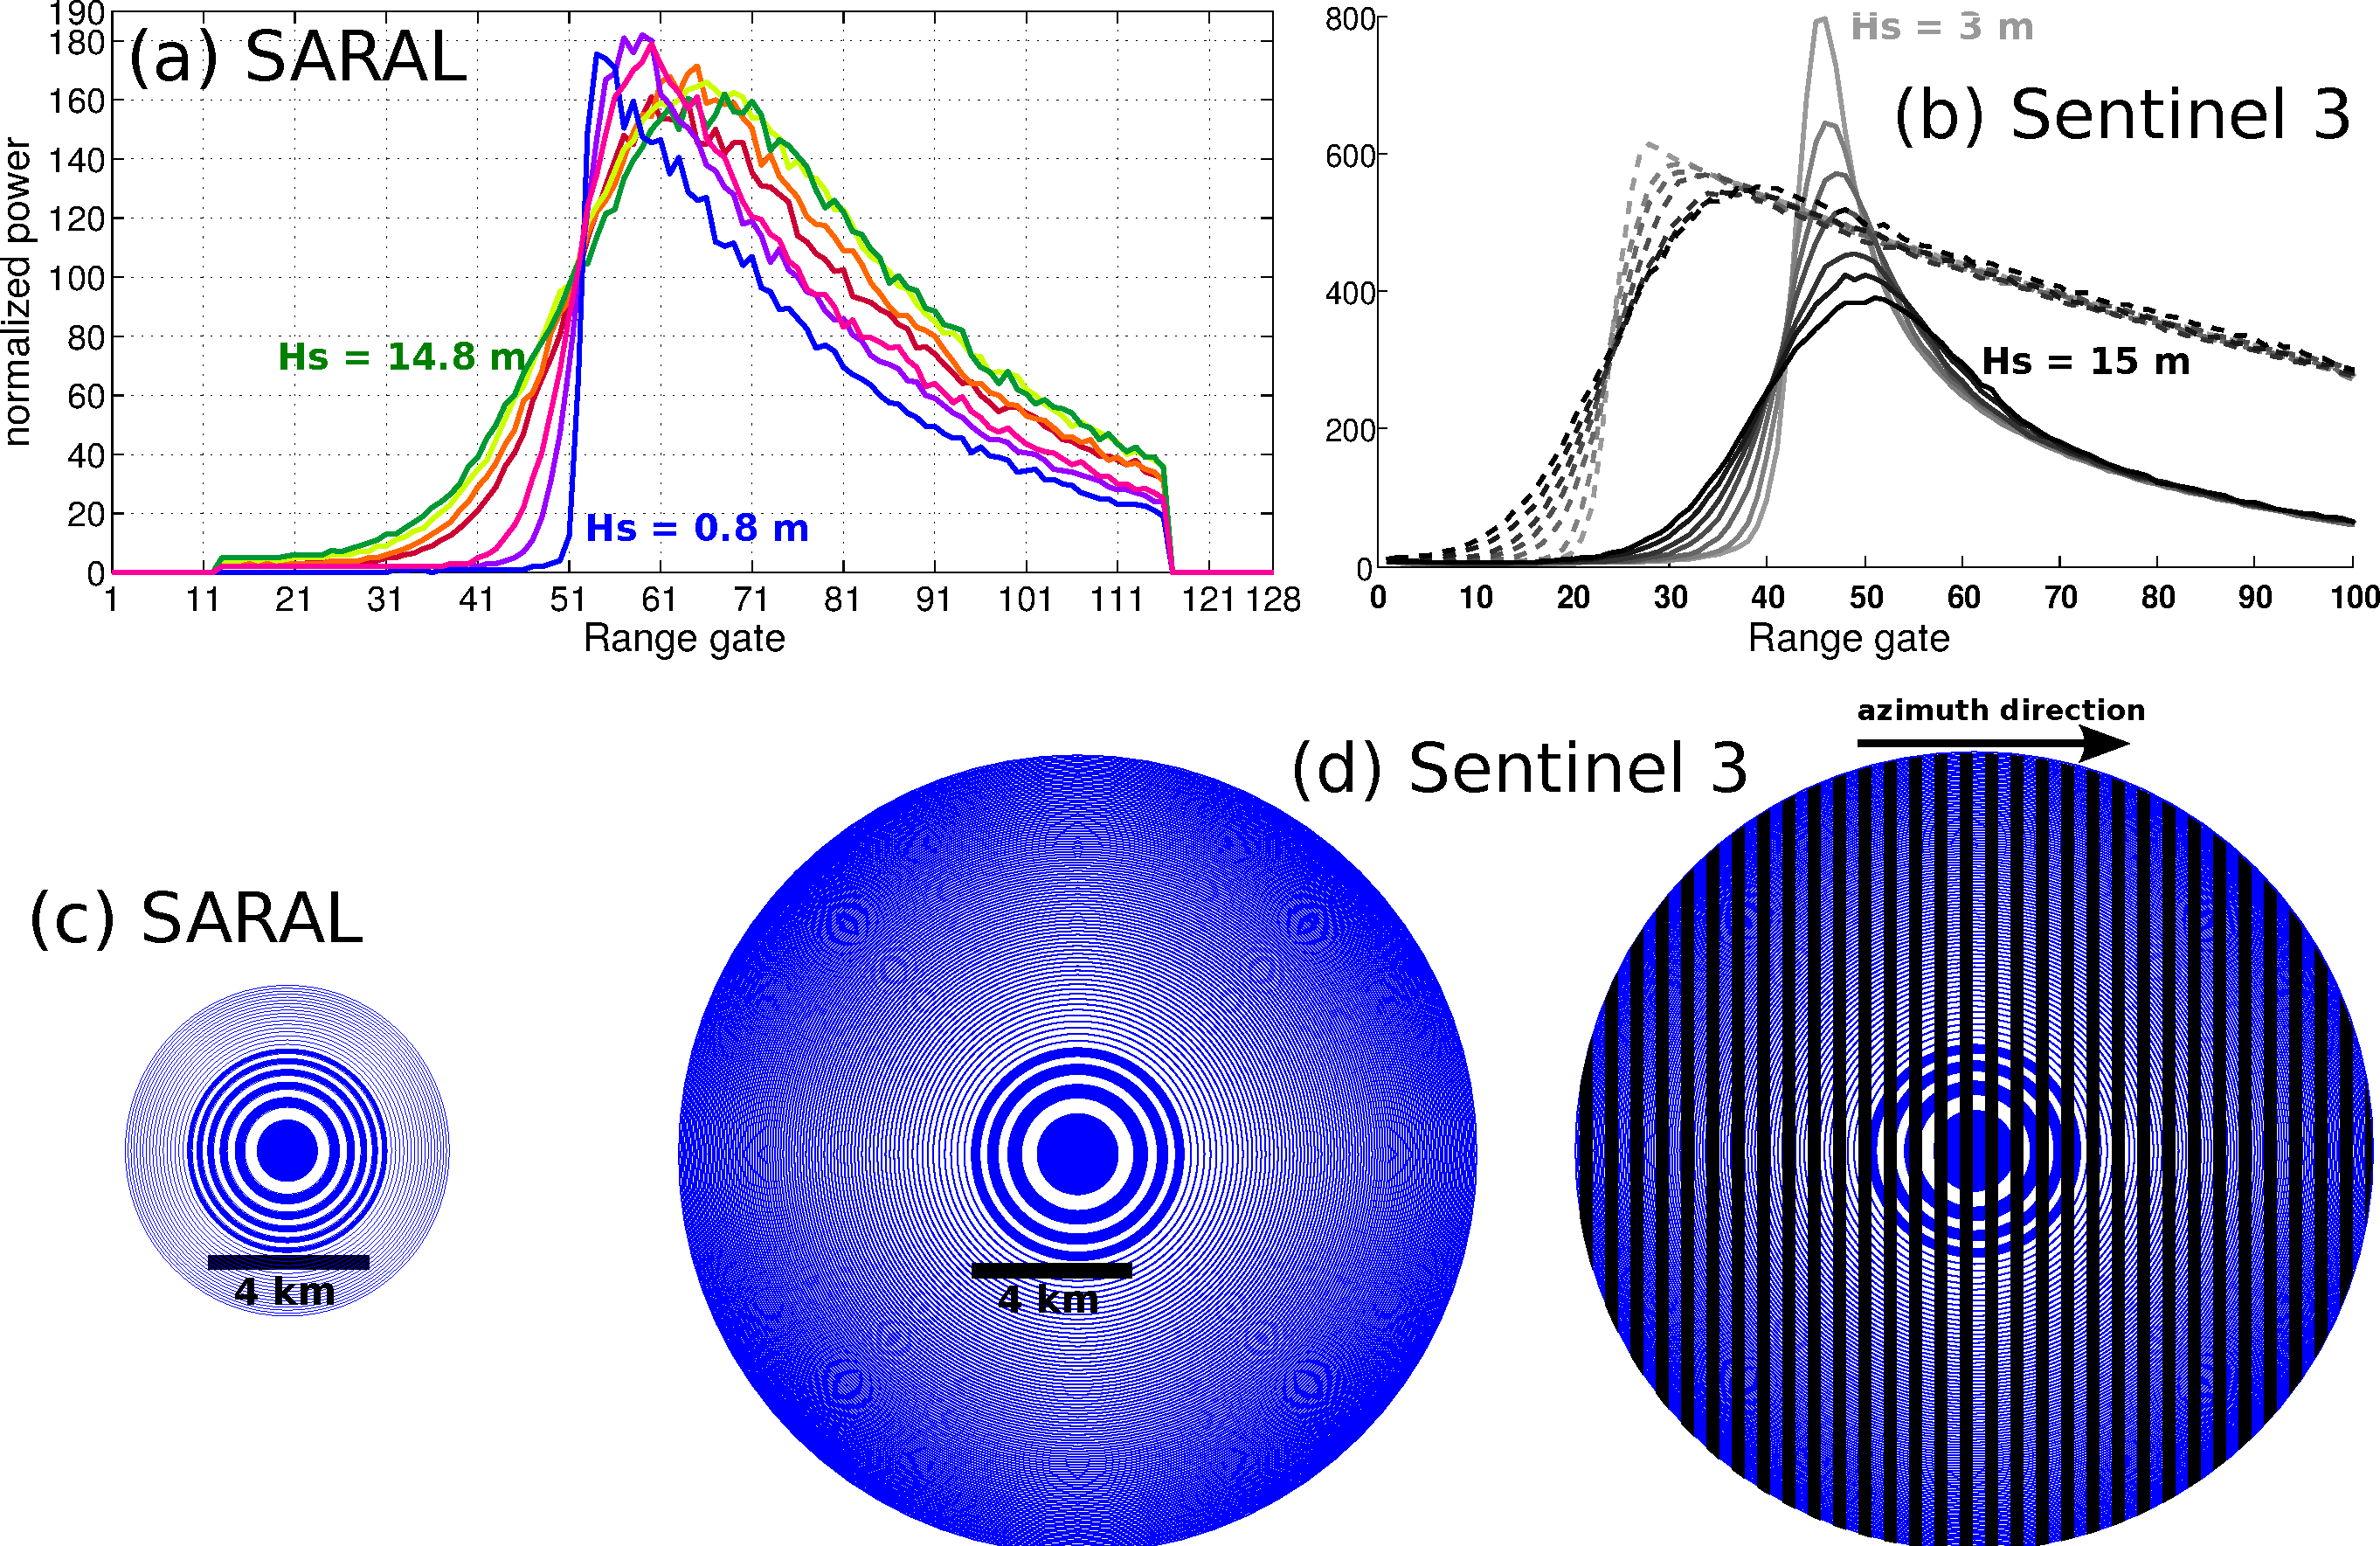
\includegraphics[width=0.9\textwidth]{FIGS_CH_SAT/dessin_footprint.pdf}}
%\vspace{3.64in}
  \caption{Altimeter waveforms and footprints}
    {Example of altimeter waveforms for different wave heights.}
    {(a) These waveforms were selected along the ascending track of SARAL/AltiKa on February 5, 2014, 
    beteen 05:29:49 and 06:20:07 UTC. Each waveform shows the the power measured by the radar as a function of time: 
    time is discretized with intervals of $2 \times 10^{-9}$~s corresponding to 
30~cm range intervals usually called `range gates'. The corresponding wave heights are 0.8, 3.2, 4.6, 9.7, 10.7, 13.2, and 14.8 m. 
Data is available from CNES/Aviso ftp. Each waveform shown here was obtained for 1~s of data, 
 as the median of 40 conscutive waveforms. (b) Similar waveforms from Sentinel 3 using delay-only (dashed) and delay-doppler (solid) for Hs = 3,5,7,9,11,13
and 15 m, for cycle 23 orbit 349, on 25 October 2017 in the Pacific. (c) Spatial coverage of footprints corresponding to the 3-dB antenna lobe pattern, for an 
unrealistic flat sea surface with a uniform roughness, with the first 11 range gates painted alternatively blue and white, 
starting from center. (d) Footprint for Sentinel 3, with the 7 seven range gates colored blue and white, with the azimuth resolution of the Doppler processing indicated by the grey stripes.
} \label{waveform}
\end{figure}
%%%%%%%%%%%%% end of figure
The first main principle of the analysis of the radar echoes is the determination  of the distance, usually called range, based on 
the delay of a radar pulse 
to travel from the transmitting antenna to the target and back to the receiving antenna. Usually the two antennas are the same piece of hardware 
and this is called a `monostatic system'. Because the radar pulse has a finite duration which limits the resolution of the time measurement, 
it is customary to use a varying transmitted carrier frequency $f_t$ that is modulated as chirps: $f_t$ is increased linearly between $f_0$ and $f_0$+$B$ during a radar pulse. As a result, the carrier frequency of the received signal $f_r$ can be used to determine the precise travel time of the received pulse, with each frequency associated to a different range $r$, with a resolution in range $dr$ that is determined by the frequency bandwidth $B$, with $dr=c /(2B)$. The actual signal at frequency $f_r$ combines echos from all ranges convoluted by the point target response \citep[e.g.][]{Halimi2013}.  

for all types of radars, it is thus better to use a larger bandwidth, 
but this is usually limited by atmospheric absorption windows or telecommunication regulations. Hence, for satellite altimeters, $B$ for the Jason altimeters is 320~MHz  
giving $dr=48$~cm. SARAL/Altika used a wider bandwidth of  
500~MHz  giving $dr=30$~cm. Because of issues with rain attenuation, all altimeters since GEOS-3 (1975-1979) have used Ku-band, except for the ongoing SARAL/AltiKa mission which uses only Ka-band.

Each radar pulse emitted by the radar antenna is reflected by an ocean area that expands with time, starting from the blue disk in the middle of figure \ref{waveform}.c, and 
expanding to the outer rings. The shape of the blue disk is only correct for a flat sea surface, and is distorted by waves as the crests give a shorter range and the troughs give a higher range. 
the radar receives echoes from wave crests firsts and wave troughs later: this difference in travel time between crests and troughs  
spreads the echoes over time. \cite{Brown1977} showed how the shape of the `waveform',  i.e. the received power return, under a number 
of simplfiying assumptions, is a convolution 
of the radar antenna pattern and the distribution of the surface elevation $\zeta$. As a result, 
the slope of the `wave form leading edge' is proportional to  $H_s$.  Because 
the rise-time typically spans a few range gates, the wave height typically comes from a region of the ocean that is between 4 and 7~km in diameter. 
In the case of the largest sea state in figure \ref{waveform}.a, the return 
power spreads over about 35 range gates, from number 26 to number 61, i.e. a distance of 10.5~m, close to the root mean square wave height
 $H_{\mathrm{rms}} \approx  H_{s}/1.4$. The power in range gates beyond 50 comes from the sea surface that is not directly 
 under the satellite but on a circle around it, and is still illuminated by the radar beam.  

Classical altimeter estimates of $H_s$ are fairly noisy when the wave height is low becase in that case $H_s$ is determined by only very few range gates, and the power in each rage gate as a random noise, also called speckle noise, caused by Rayleigh fading of ocean echoes that are coming from ranges spread over a distance much greater than the electromagnetic wavelength hence with random phases that randomy cancel \citep{Quartly&al.2001}. 
\cite{DeCarlo&al.2023} showed that wave groups introduce fluctuations in the estimated values $\widehat{H}_s$ that are proportional to $H_s$ and the spectral peakedness parameter $Q_{kk}$, these fluctuations can be dominant for the largest wave heights. 



Another interesting parameter that can be derived from the waveforms is the mean square slope (mss). Indeed, 
the backscattered power $\sigma_0$ is nearly inversely proportional to the mss \citep{Vandemark&al.2002}. 
For display purposes the waveforms shown in figure \ref{waveform} have been scaled: you can see that the noise level (power in gates 11 to 21) which should be nearly the same for 
all sea states is scaled to lower values for lower sea states that generally have low values of both $H_s$ and mss.  
Because the mss is not a very common parameter in applications, many authors have derived empirical estimates of peak or mean  periods from $H_s$ and $\sigma_0$. Also, the mss is a good proxy for the wind speed \citep{Cox&Munk1954}.



It should be noted that the main application of the altimeters was the mapping of the sea surface height (SSH) for the determination of the geoid, tides and dynamical topography. The measured
 SSH can be much more precise than $dr$, thanks to averaging. Waves play an important role in the estimation of the SSH because of a range bias induced by wave non-linearities that induce a correlation between the surface slope (and this its brightness for the radar) and the surface elevation. This is known as 
 the sea state bias, and on average it is of the order of
 3~\% of Hs \citep[e.g.][]{Minster&al.1992}. 
 
 Also, because $H_s$ and SSH are estimated jointly using a parametric fit to the waveform, there are important correlated errors in the two parameters \citep[e.g.][]{Dibarboure&al.2014,DeCarlo&al.2023}. 
 As a result, without any particular editing or fitting of the waveforms, the variability of $H_s$ at scales shorter than 80~km is 
 expected to be mostly due to the error in the fitting procedure that can be associated to non-uniform radar backscatter and other effects. Recent methods have been developed to reduce that noise and filter it \citep{Passaro&al.2015,Quilfen&Chapron2019}.
 %%%%%%%%%%%%% figure
\begin{figure}[htb]
\centerline{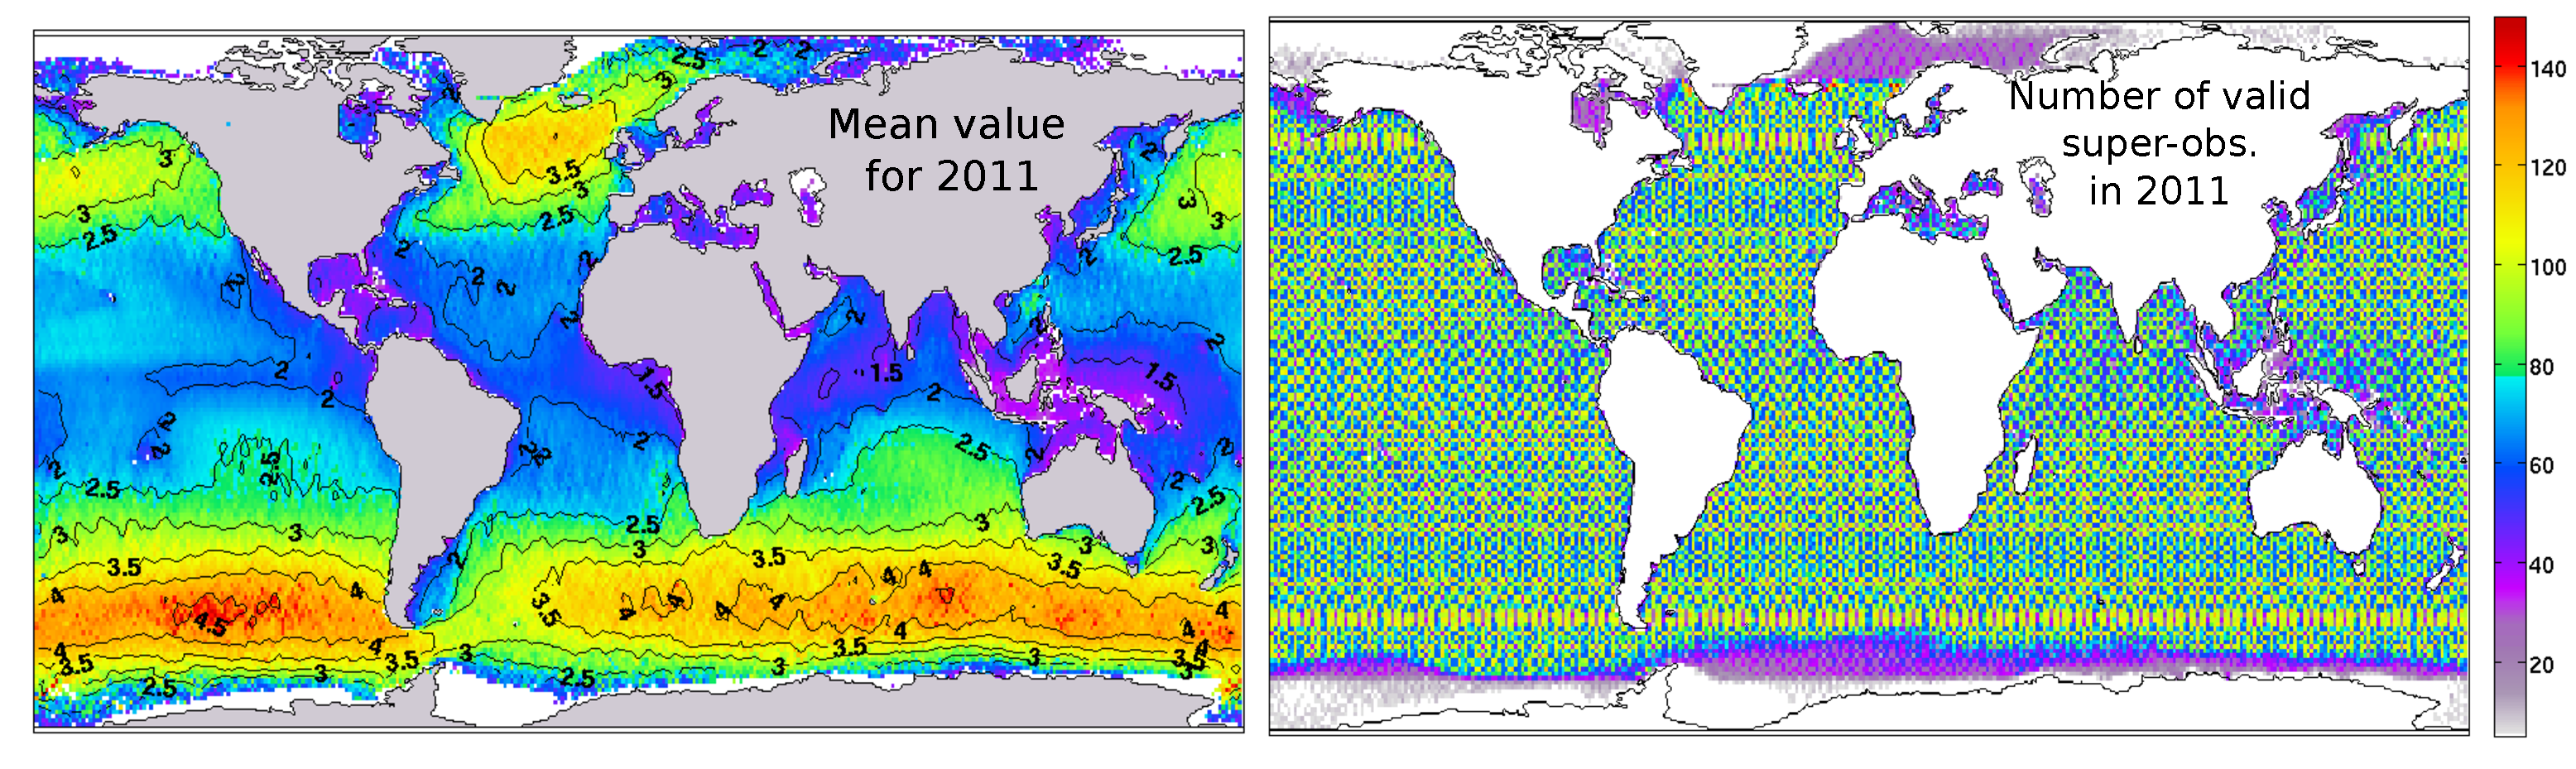
\includegraphics[width=\textwidth]{FIGS_CH_SAT/altimetre_cartes2011.pdf}}
%\vspace{3.64in}
  \caption{Global coverage of satellite altimeters}
    {Over one day, the 3 satellites Jason 2, Cryosat 2 and SARAL/AltiKa covered all the oceans and seas with a density high enough to capture all the 
important storms. In a year, the full ocean is covered at a resolution of 1 degree in latitude and longitude.  
 Data provided by ESA and CNES and processed by Ifremer. The spatial 
cover depends on the orbits shape. The number of tracks per 1 degree x 1 degree box (bottom panel) varies
from 20 to 160 over a year: the coverage is less frequent close to the pole because Jason 2 has a more oblique orbit that does not cover the 
latitudes beyond 66 degrees. Also, sea ice  produces echoes that differ from those of water and prevent the estimation of the wave height.} 
\label{fig:altimeter_coverage}
\end{figure}
%%%%%%%%%%%%% end of figure

Details will vary with different instruments, and here we will use the most simple case of radar altimeters. It was shown by \cite{Chelton&al.1989} that the sea echoes that contribute to the rising part of the waveforms, as shown on Fig. \ref{waveform}, are within a radius $r_C$ of the nadir, the point on the sea surface that is vertically below the satellite, with 
\begin{equation}
    r_C =\sqrt{\frac{ 2 h_o H_s+ 2 \delta_R}{1+h_o/R_E}} \label{eq:rC}
\end{equation}
where $h_o$ is the satellite orbit height above the ground, $R_E$ is the Earth radius and $\delta_R$ is the range resolution of the altimeter.  

\subsection{delay-Doppler altimetry}\label{section:delay-Doppler}
Another principle that can be used to refine the position and/or to measure the velocity of targets along the satellite flight path is the Doppler effect: fixed targets ahead of the radar are moving towards it, and hence have a higher frequency, while fixed targets that are behind along the satellite path 
are moving away, giving a lower radar frequency. Typical low Earth orbits give a satellite velocity around $V=7$~km/s. Hence, a Ka-band system at 36~GHz frequency will see a Doppler shift
of the order of $V f_r/c = 840$~kHz, which is further reduced by the incidence angle $\theta_r$. For a 0.5$^\circ$  antenna aperture, $\theta_r$ will 
normally vary between 0 and 0.5$^\circ$,  and the Doppler will be limited to 7.3~kHz.  

The main benefit of Delay-Doppler altimetry is the increase of the number of "independent looks" of the sea surface, which helps reduce Speckle noise, but cannot do anything about the true geophysical variability induced by wave groups. Delay-Doppler altimetry has also been developed to separate echoes along the track, which is particularly useful for measuring sea ice freeboard at the edges of sea ice leads, hence its first implementation on Cryosat-2. 


A slicing of the radar echoes according to their Doppler shift allows a high-resolution mapping of the surface along the satellite track. 
This principle is used on  Cryosat-2, Sentinel-3, and Sentinel-6 (Mike Freilich) with a standard processing giving 300~m resolution along the track, as shown on figure \ref{waveform}.d. In that case the basic 
data has now one extra dimension, making a `stack' of waveforms. For practical purposes, this stack is converted to a single `SAR mode' waveform, such as the solid lines 
shown in figure \ref{waveform}.b. 
At such a  resolution, the surface elevation due to  very long swells propagating along the track can be resolved. 
A natural limit to this along-track resolving power is the fact that the sea surface is moving up and down with the waves. Indeed, an orbital velocity 
of $w=2$~m/s gives a $u f_r / c=$ Doppler shift that can be mis-interpreted as a difference in incidence angle $\theta_r$ such that  
$(u f_r / c)=(V \sin\theta_r  f_r/c)$, this corresponds to a horizontal displacement $u H_r/V \simeq 200$~m for a radar altitude 
$H_r = 800$~km. 


%\subsubsection{Interferometric systems}



 \subsection{Synthetic Aperture Radars (SARs)}
As  explained, in section \ref{delay}, the separation of echoes in the range direction is easily achieved by combining the delay and frequency modulation of 
the chirped radar signal, with a resolution in distance that is thus controled by the frequency bandwidth. 
In the other direction (azimuth), the simultaneous echoes can be separated by their Doppler shift. 
This is perfect if targets are fixed relative to the ground, and a 
very good resolution can be obtained, both in the range and azimuth directions (about 10~m for Envisat, 5~m for Sentinel 1 in wave mode and 1~m in spotlight mode for TerraSAR-X). This processing 
produces a  map of the surface 
backscatter in delay-Doppler coordinates. Unfortunately these positions are distorted from  true geographic positions when the surface is moving toward the 
radar. With a vertical velocity $w$, targets are displaced by $\delta=w \cos \theta_i  R/V$ along the azimuth direction. With a Sentinel-1 altitude $H_r = 693$~km  and a typical speed over ground $V=7.5$~km/s, when looking at an incidence angle of 23$^\circ$ the distance $R$ is close to\footnote{That approximation assumes a locally flat Earth. The exact value is obtained from the law of cosines in the triangle made of the satellite position, the target position and the center of the Earth, i.e. $R^2 + 2 R R_e \cos \theta_i +R_e^2 - (H_r +R_e)^2=0$, where $R_e$ is the radius of the Earth.} $H_r/\cos \theta_i$ and the 
factor $H_r/V$ is about 92~s$^{-1}$, i.e. a very small velocity  $w= 10$~cm/s gives a displacement in azimuth of $\delta=9.2$~m. 
A high speed train traveling at 100 m/s along tracks at $45^\circ$ with the range direction at an azimuth angle of 23$^\circ$ has a radial velocity of 28~m/s, would be displaced 2.7~km in the azimuth direction, at a location that is 2~km \textit{away} from the tracks!
%Figure \ref{fig:SAR_cars} shows an example of targets displaced from their true locations according to their azimutal speed. 
%
%
%%%%%%%%%%%%% figure
%\begin{figure}[htb]
%\centerline{\includegraphics[width=0.7\textwidth]{FIGURES/SAR_cars.pdf}}
%  \caption{Where is the fast car? it is in the optical picture, but out of the SAR `image'!}
%    {Images of cars with different velocities along an airport runway in a nominally processed radar image (left) and 
%a reference optical image (right), adapted from \cite{Palubinskas&al.2005}. The SAR acquisition was made from a Do-228 aircraft 
%flying at only 88 m/s and altitude 3.94~km, giving a ratio $H_r/V=44$~s$^{-1}$.} 
%\label{fig:SAR_cars}
%\end{figure}
%%%%%%%%%%%%%% end of figure


%%%%%%%%%%%%% figure
\begin{figure}[htb]
\centerline{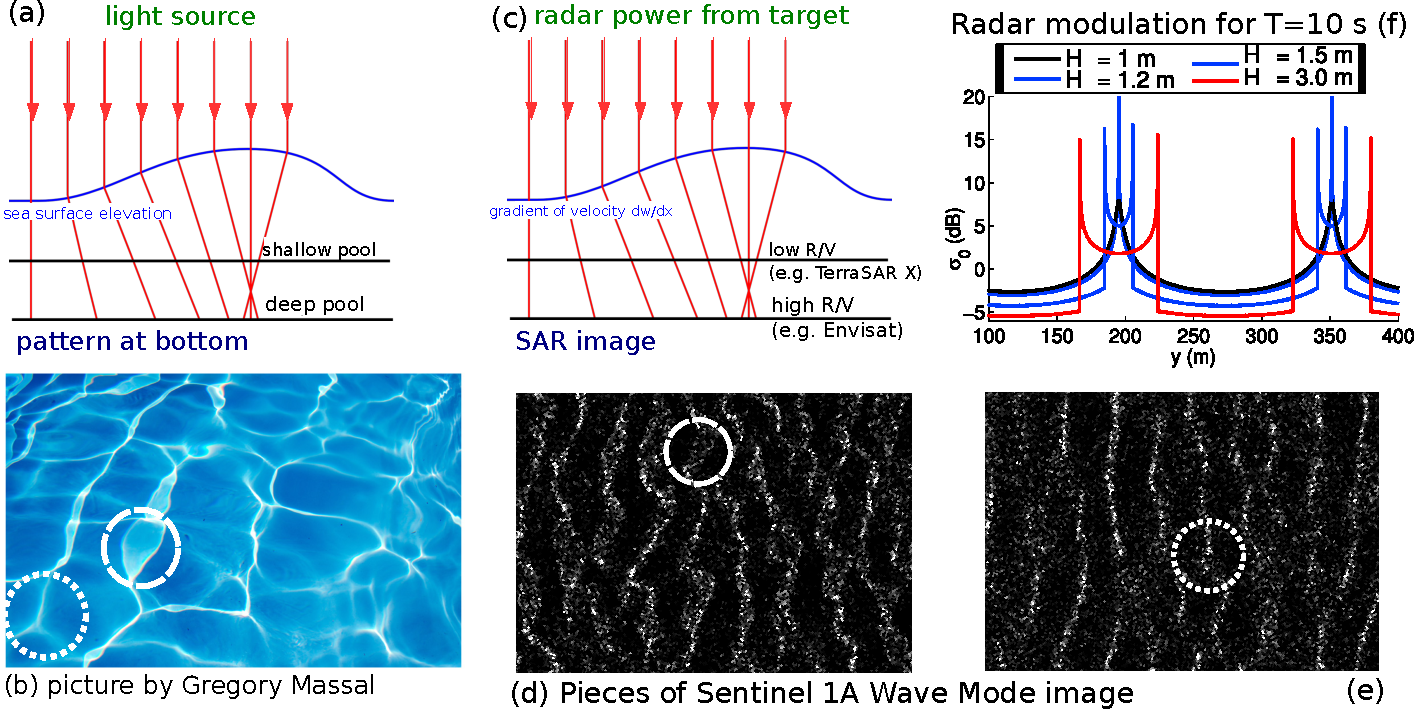
\includegraphics[width=0.8\textwidth]{FIGS_CH_SAT/dessin_fig1_landscape.pdf}}
%\vspace{3.64in}
  \caption{Patterns in SAR images}
    {Analogy between (a,b) light patterns at the bottom of a shallow pool, and (c,d,e) velocity bunching effects
in SAR images of ocean waves. (d) and (e) are taken from a wave mode Sentinel 1A image, acquired on 9 September 2014 at 04:48:16 UTC, 
at 10 and 35~km inside of the sea ice. In (d), almost all crests are doubled, for example in the region within the dashed circle. 
In (e) the lines are less bright and not doubled (for example within the dotted circle). This is easily simulated, as shown in (f), with the variations of image intensity
expected from a sinusoidal monochromatic wave of wavelength 156~m \citep[Adapted from ][]{Ardhuin&al.2017}.} 
\label{fig:SAR_pool}
\end{figure}
%%%%%%%%%%%%% end of figure
In the case of  waves motion a velocity bunching effect appears, the echoes on the image are shifted from their actual
position depending on the surface velocity towards the satellite creating a pattern of brighter areas, where the displaced targets are `bunched 
together', and darker regions. This mechanism is often the main cause of the wave-induced $\sigma_0$ modulation in the open ocean. 
In ice-covered water, this is probably the only mechanism present that creates wave patterns in SAR images. This bunching in the azimuth direction is very 
similar to the light patterns at the bottom of a shallow pool that are caused by light refraction, as illustrated in figure \ref{fig:SAR_pool}. 

%%%%%%%%%%%%%%%%%%%%%%%%%%%%%%%%%%%%%%%%%%%%%%%
%\begin{figure}[htb]
%\centering
%\includegraphics[width=\linewidth]{FIGURES/Nov1_for_book.pdf}
%\caption{Context of the  Sentinel-1A image acquired on November 1st, 2015, at 17:23 UTC, and available in situ data. The full image at 
%full resolution can be viewed at \href{http://bit.ly/22JFruo}{http://bit.ly/22JFruo}. (a) SAR-derived
%roughness (gray scale) showing open water between the Alaska shoreline, to the West of Barrow, and the measurement locations in the red box. 
%(b) Location of the R/V Sikuliaq and some of the measurement buoys. Note that buoy S15 is in open water. 
%(c) piece of the SAR image around the buoys S13 to W3. (d)  Directional spectrum estimated from S15 data using the Maximum Entropy Method.
%(e) Comparison of spectra derived from in situ data and the SAR image around buoy S13 and buoy W3. In each panel the spectrum at the offshore buoy S15 is 
%indicated for reference. The 'cut-off' effect is the reduction of wave spectrum according to eq. (\ref{eq:cutoff}). Adapted from \cite{Ardhuin&al.2017}.}
%\label{fig:nov1}
%\end{figure}
%%%%%%%%%%%%%%%%%%%%%%%%%%%%%%%%%%%%%%%%%%%%%%%
In the case of a monochromatic wave train propagating in the azimuth ($y$) direction, with wavenumber $k_y$, and not located right under the satellite but at an icidence angle $\theta_i$, 
the target displacement in the SAR image due to the velocity towards the satellite is 
\begin{equation}
 \delta = \left ( W \cos (k_y  y - \sigma t) \cos \theta_i  + U \sin (k_y  y - \sigma t) \sin  \theta_i  \right) H_r/(V \cos \theta). \label{eq:delA}
\end{equation}
where $U$ and $W$ are the amplitudes of the horizontal and vertical velocities given by eqs. (\ref{vitesse})-(\ref{eq:w}). 

Assuming a uniform radar power scattered from the sea surface $\sigma_0$, and taking the $y$ dimension  along the azimuth, 
the SAR image intensity is the incoherent sum at the displaced positions $y'$ of the power coming from the true pixel positions $y$, it is thus given by the inverse of Jacobian of the SAR displacements 
$y \rightarrow y'=y+\delta$, \citep[see eq. 21  in][]{Hasselmann&Hasselmann1991}, 
\begin{equation}
 J = \left|dy'/dy\right|,
\end{equation}
for a monochromatic wave of amplitude $a$ it is, 
\begin{equation}
I'_{SAR}(y) = \sigma_0/J = \sigma_0 / \left|1 -  C_{AR}  \sin( k_y y- \sigma t) \right|\label{ISAR}.
\end{equation}
The important parameter for image patterns is the coefficient $c$ in \cite{Alpers&Rufenach1979}, 
\begin{equation}
  C_{AR}=k_y (W + U \tan \theta_i) H_r/V.\label{eq:CAR_def}
\end{equation}


 For $C_{AR} << 1$, eq. (\ref{ISAR}) can be linearized, but as $C_{AR}$ increases, the SAR displacements become strongly nonlinear and for $C_{AR}= 1$, 
 the Jacobian is zero and $I'_{SAR}$ becomes infinite just like the light intensity at the focal point of a lens. 
In our figure 1.f, with a wave period of 10~s traveling in the azimuth direction, $C_{AR}= 1$  corresponds to an amplitude of the elevation $a=0.42$~m, 
which, for random waves of the same energy would be a significant wave height $H_s=4\sqrt(a^2/2)=1.2$~m. 
For $C_{AR} > 1$, each bright line becomes a doublet. The two lines of the doublet progressively drift apart as the amplitude increases, pulling 
the minimum intensity to lower and lower values, up to the point where lines 
from different doublets meet, at $ C_{AR} \simeq 4.6$. Beyond this value there is no region of very low intensity anymore. 
%For waves  in  sea ice, this can be inverted for  $C_{AR}$ less than about 2 to give a map of orbital velocities and from that the wave spectra \citep{Ardhuin&al.2016b}.

In practice, except far inside the  sea ice cover, there are also short wave components in the wave spectrum $E(\kb)$. From a SAR processing point of view, 
these short waves are equivalent to Gaussian random vertical oscillations 
of $<v^2>$ leading to random displacements in the SAR image that are larger than their wavelengths and that do not produce any pattern. These short 
waves also reduce the contrast of longer components. \cite{Hasselmann&Hasselmann1991} gave a theoretical derivation of the impact of random waves on a SAR image spectrum $E_S(\kb)$,
their eq. (55), with a simplified derivation by \cite{Krogstad1992}. In practice the short wave effect is a reduction in the image spectrum by an exponential factor,  
\begin{eqnarray}
 E_S(\kb)&\simeq& \exp(-k_y^2 <v^2> H_r^2/V^2) E_l (\kb) = \exp(-k_y^2 \lambda_c^2/(2 \pi)^2 ) |M_S|^2 \left(E(\kb)+E(-\kb)\right)/2 , \label{eq:cutoff}
\end{eqnarray}
in which $E_l(\kb)$ is a linearized spectrum, based on a modulation transfer function $M_S$ that includes a linearized velocity bunching term, a hydrodynamic term due to the short scattering waves modified by 
longer waves, and a tilt term due to the change in local slope along long waves \citep{Hasselmann&al.1985,Hasselmann&Hasselmann1991}. All terms depend on the incidence angle, 
and these last two terms depend on the polarization of radar waves, horizontal or vertical, and on wind speed and wave age. 
The image is 
completely blurred at the scale of the random displacements and the resolution of 1 or 5~m is useless.


The azimuthal cut-off wavelength is $\lambda_c =  2 \pi \sqrt{<v^2>} H_r/V$, in which $<v^2>$ is the orbital velocity variance.  This cut-off effect is so dominant that it can 
actually be used to measure the surface orbital velocity variance from SAR images \citep{Stopa&al.2016}. A minor difficulty is the separation of the part of the wave spectrum that 
produces patterns in the SAR image and the shorter part that only introduces blurring. Looking at many ERS SAR data, \cite{Kerbaol1997} concluded that, in the case 
of a wind sea, the velocity variance $<v^2>$  should be restricted to waves shorter than a factor $f_L$ times the peak wavelength, with $f_L \simeq 0.33$ for a mean short wave direction 
in the range direction and  $f_L \simeq 0.15$ in the azimuth direction.  

Combining all these effects with some empirically derived MTFs, it was possible to estimate the heights of swells within 25\% of buoy measurements using 
wave mode data from Envisat \citep{Collard&al.2009}. The full significant wave height, including the waves shorter than $\lambda_c$ that are not resolved in the 
SAR image, can also be estimated by combining all image parameters \citep{Li&al.2011}. 






Several aspects of SAR processing are the subject of active research, including the measurement of high winds or currents, and improvements in the estimates of wave 
parameters in particular in ice-covered regions. 

%Figure \ref{fig:nov1} shows an example of waves around the ice edge: in the water (buoy S15), the waves cannot be seen by the SAR 
%because, with a peak wavelength of 100~m, they are much shorter than the 290~m cut-off wavelength. Waves only appear in the ice with an %increasing SAR spectral 
%density which is not due to an increase in wave height, but a reduction in the cutoff wavelength from $\lambda_c = 114$~m at S13 to  $\lambda_c = 87$~m at W3. Hence a correct estimation 
%of $\lambda_c$ is critical for a proper estimation of wave heights either in the open ocean or in ice-covered water. Another important practical problem, especially in ice-covered 
%region, is the presence of non-wave features in the image: boats, slicks, variations in wind speed, leads in ice... these usually show up in the low frequency part of the spectrum, 
%and, in figure \ref{fig:nov1} they probably are the reason for the spurious bump at $f=0.1$~Hz. 
 
Since SAR images are characterized by high resolution (5~m in the Sentinel-1 wave mode, 10~m in Interferometric Wide swath mode), and large coverage, they provide a unique opportunity 
to measure the spatial patterns in the wave field, as shown on figure \ref{SAR_exemple}.

%%%%%%%%%%%%% figure
\begin{figure}[!h]
\centerline{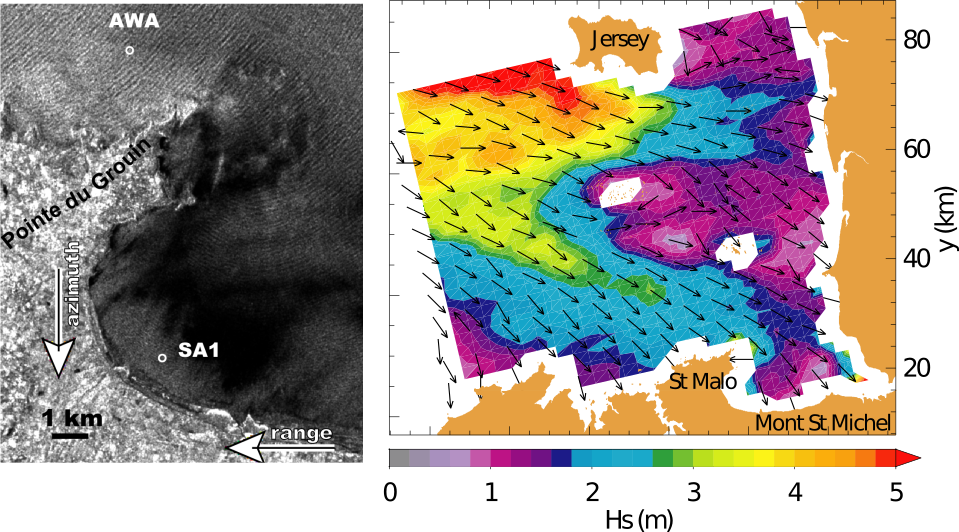
\includegraphics[width=0.8\textwidth]{FIGS_CH_SAT/Image_SAR_Cancale2.png}}
\caption{Left: Sample of a SAR image, recorded by Envisat  on March 9 2003, over French coast. The grey level is a function of the radar cross section that is modulated by waves. 
Right: Full image processed into wave spectra, with significant wave height and peak direction. AWA et SA1 are positions of in-situ instruments, 
used for validation \citep{Collard&al.2005}.}
\label{SAR_exemple}
\end{figure}
%%%%%%%%%%%%% end of figure



\subsection{SAR Across-track Interferometry: SWOT and near-nadir range bunching effects}
Compared to the SAR systems on Envisat and Sentinel-1 described above, the KaRIN instrument on SWOT has two very different features: first it measures at incidences very close to the vertical (nadir), and second it actually has 2 SAR systems forming a cross-track interferometric baseline. This means that in addition to the usual SAR imagery (a little unusual with KaRIN due to their incidence angles) we also get interferograms from the two SAR receivers on KaRIN, which provide a wealth of information: 
\begin{itemize}
\item the mean phase of the interferogram is related to the distance between the radar and the reflecting target, hence the sea surface elevation, which contains the geoid, the dynamic height, tides, internal waves... but also those wind-generated waves that are longer than the SAR pixel, as shown on Fig. \ref{fig:SWOTswell}. 
\item the noise of the interferometric phase is related to the distribution of these distances within a resolution pixel, hence the significant wave height of the waves that are not resolved by the image. 
\end{itemize}

When trying to analyse SWOT data at small scales, it is thus really important to understand what is resolved, what is not, and how the unresolved surface elevations give spurious signals in the resolved part: indeed the imaging of the surface at near-nadir angles meas that all targets that have the same range will fall in the same pixel, even though they are not at the same $(x,y)$ position. This leads to a fairly nonlinear image-blurring or image-enhancing effect called "range-bunching": just like velocity bunching, which distorts or enhances the image in the azimuth direction, range bunching leads to distortions and blurring in range. Figure \ref{fig:SWOTswell} shows some example of wave signatures in SWOT surface elevation maps, that still have to be analyzed quantitatively.
%%%%%%%%%%%%% figure
\begin{figure}[htb]
\centerline{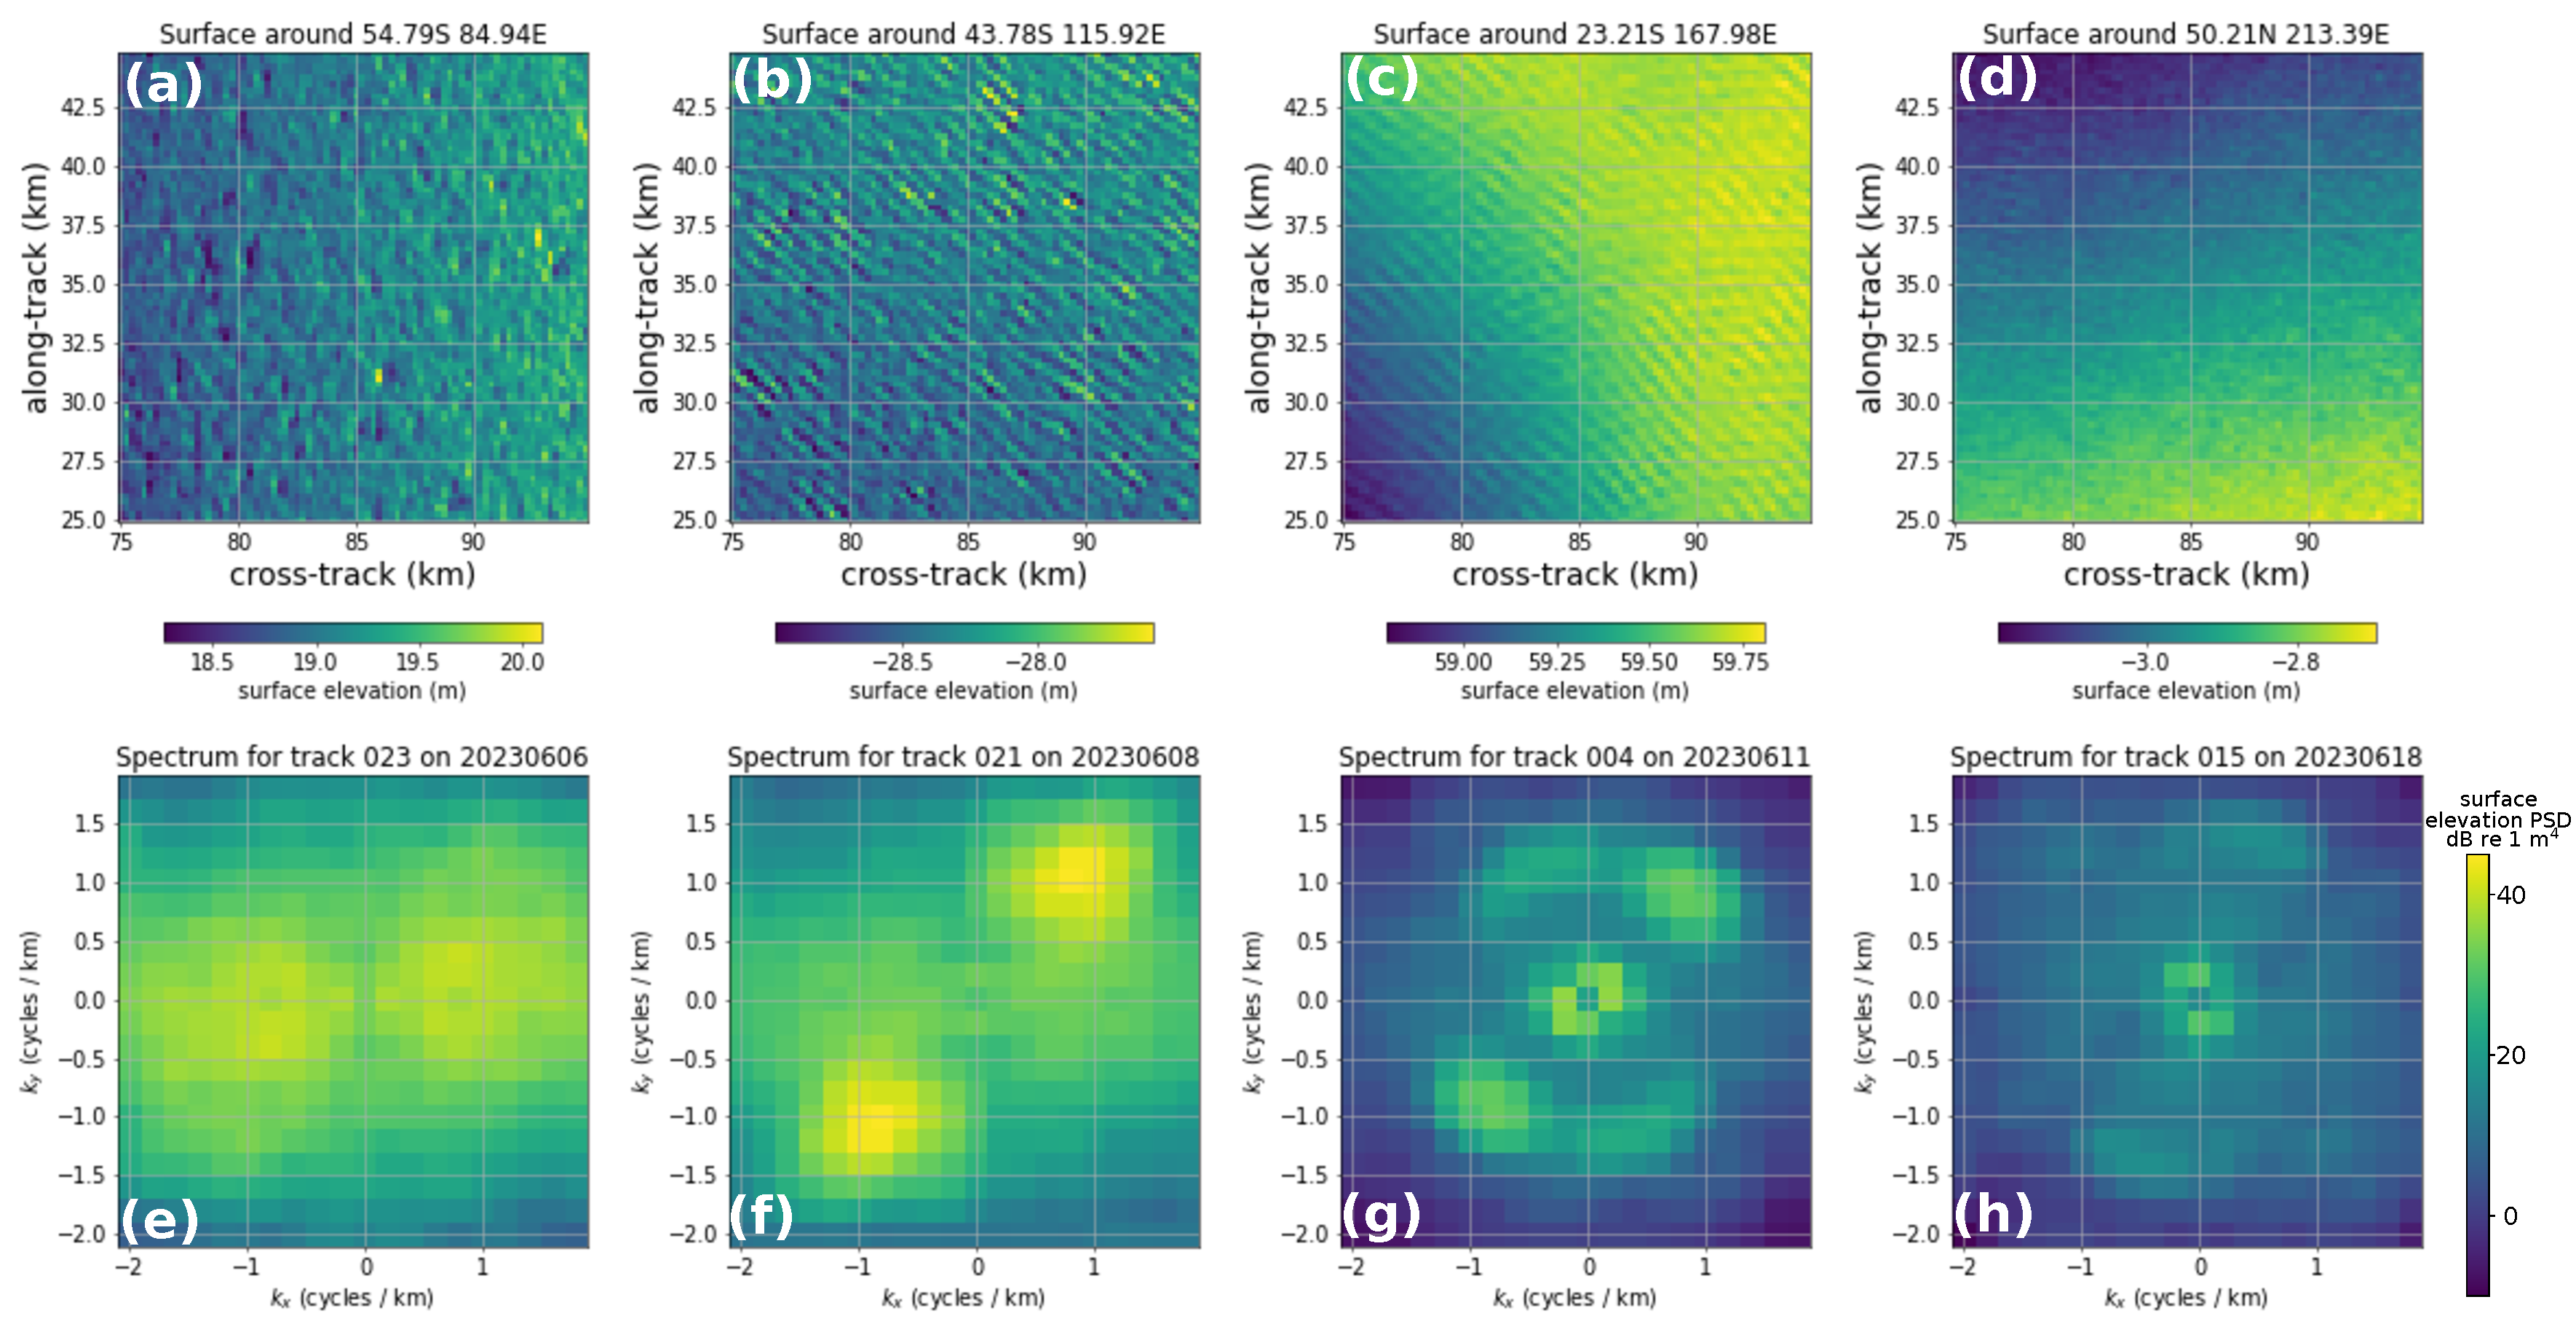
\includegraphics[width=\textwidth]{FIGS_CH_SAT/SWOTSWELL.pdf}}
\caption{Following swells with SWOT, from storm to the antipodes}{Top: small pieces (20 by 20 km) of SWOT data, bottom: corresponding surface elevation spectra $E(k_x,k_y)$, these are double-sided spectra. Left: in the storm on June 6 2023, south of Kergulen islands with strong range bunching effect. Next: large swells South of Australia, June 8. Next: refraction and diffraction over Antigonia seamount, south-east of New Caledonia, June 11. Right: small amplitude swells at ocean station Papa, Gulf of Alaska, on June 18, after 17,000~km of propagation.}
\label{fig:SWOTswell}
\end{figure}
%%%%%%%%%%%%% end of figure
You may look at the work by \cite{Peral&al.2015} before a more detailed summary appears in this section or a new chapter. 

\subsection{The wave spectrometer and the matching wavefront technique}
Whereas a SAR resolves the wave patterns in an image to produce a wave spectrum, 
it is possible to measure the 2D wave spectrum from a combination of 1D wave spectra. 
%%%%%%%%%%%%% figure
\begin{figure}[htb]
\centerline{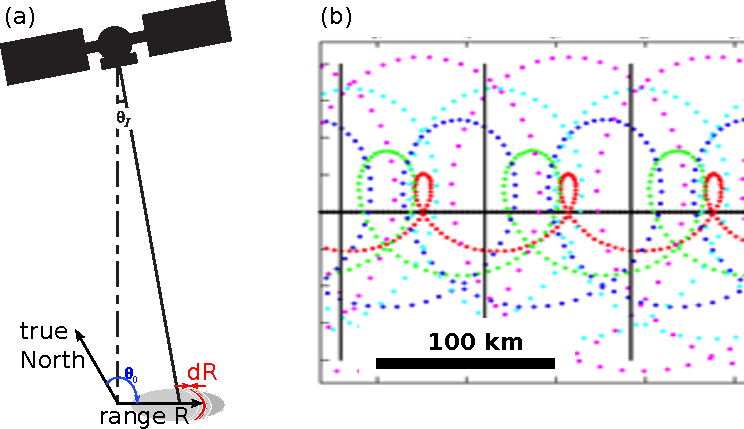
\includegraphics[width=0.4\textwidth]{FIGS_CH_SAT/CFOSAT_v2.pdf}}
\caption{Measurement principle  the SWIM radar that on CFOSAT. (a) geometry of the measurements for one cycle 
in direction $\theta_0$. The resolution in range $dR$ is of the order of 10~m, but the azimuth resolution is 18 km. Using different incidence angles $\theta_I$ (0, 2, 4, 6, 8 and 10 degrees) 
and rotating around the nadir provides estimates $E(k,\theta_0)$ in all direction $\theta_0$. (b) Coverage of the SWIM instrument on CFOSAT: each colored dot is the center 
of a 19~km diameter footprint.}
\label{CFOSAT}
\end{figure}
%%%%%%%%%%%%% end of figure

When echoes are combined from narrow strip in range (red band in figure 
\ref{CFOSAT}.a), the Fourier transform of these echoes in the range direction selects only the modulations by waves that are perfectly aligned with the direction 
$\theta_0$ to which the radar is looking, all other components cancel out.  Hence, the Fourier analysis of radar echoes provides a 1D spectrum  $E(k,\theta_0)$  
in the look direction. 
A successive acquisition in different directions provides the full directional spectrum $E(k,\theta)$.  
This is the principle of the wave spectrometer and it has been demonstrated with the airborne instrument
RAWS, developed by NASA \citep{Jackson&al.1985}, STORM and KuROS developed jointly by CNES and CNRS \citep{Hauser&al.1992,Caudal&al.2014}.
The first satellite wave spectrometer is SWIM, and it flies on the China-France Ocean Satellite (CFOSAT, Figure \ref{CFOSAT}), which was launched on October 29, 2018 \citep{Hauser&al.2021}. SWIM is unique in providing wave spectra co-located with classical altimeter measurements, allowing a a much better understanding of historical altimeter data and their along-track variability \citep{DeCarlo&al.2023}, as detailed in chapter \ref{ch_groups}. 

%For larger incidence angles, the measurements cover a larger area of the ocean, but there is more sensitivity to the wind speed in the radar back-scatter. Hence, the SWIM  design is limited to 10 degrees of incidence. A larger incidence also requires a more powerful radar, because the reflectivity decreases with incidence angle. 

It is also possible to analyze the Doppler of the backscattered signal, as demonstrated with KuROS \citep{Caudal&al.2014}, but this is best done with a narrower antenna pattern as used from space. This additional measurement allows to remove the 180 degree ambiguity on the 
wave propagation direction, but it also provides an indepedant measuremnt of the wave spectrum via the orbital velocities, and finally it contains the signature of 
surface currents.  This Doppler capability to measure currents was included in the SKIM concept \citep{Ardhuin&al.2019e} and demonstrated with airborne measurements \citep{Marie&al.2020}.



\cleardoublepage
\chapter{Measured wave evolution: main parameters and wave spectra}\label{ch3}
A casual observation of the sea is enough to figure out that, the stronger the wind, the higher the height $H$ and length $L$
of the waves. From one location to another, it is also obvious that $L$ and $H$ change with the water body: a large lake can hold bigger waves than a pond, and waves in the 
Pacific, the largest water body on Earth, can reach close to 40 m high, with wavelengths above 600 m. Finally, within the same water body, the heights and lengths increase 
when moving downwind. The present chapter aims at providing a quantitative summary of observed wave properties, including useful empirical prediction formulae. These were the basis of
wave forecasting methods \citep[e.g.][]{Pierson&al.1955} before the advent of numerical models \citep{Gelci&al.1957}.

\section{Wind-sea growth}
A wide range of visual observations were systematically gathered by Sverdrup and Munk in 1941
in order to come up with a wave forecasting method for the U.S. Navy, faced with the delicate task of 
landing on the swell-battered beaches of Morocco. This work, initially classified, was only published as 
a landmark report after the war \citep{Sverdrup&Munk1947}. The miscelaneous observations were organized 
thanks to dimensional analysis with wave variables $H$ and $T$ expressed as a function of the wind speed 
$U_{10}$ as measured at 10 m above the sea surface, the fetch 
$X$, the duration $t$ over which of the wind has blown and the acceleration of gravity $g$. The fetch $X$ is the length 
of the region over which the waves have been generated. 

%%%%%%%%%%%%%%%%%%%%%%%%%%%%%%%%%%%%%%%%%%%%%%%%%%%%%%%%%%%%%%%%%%%%%%%%
\begin{figure}[htb]
\centerline{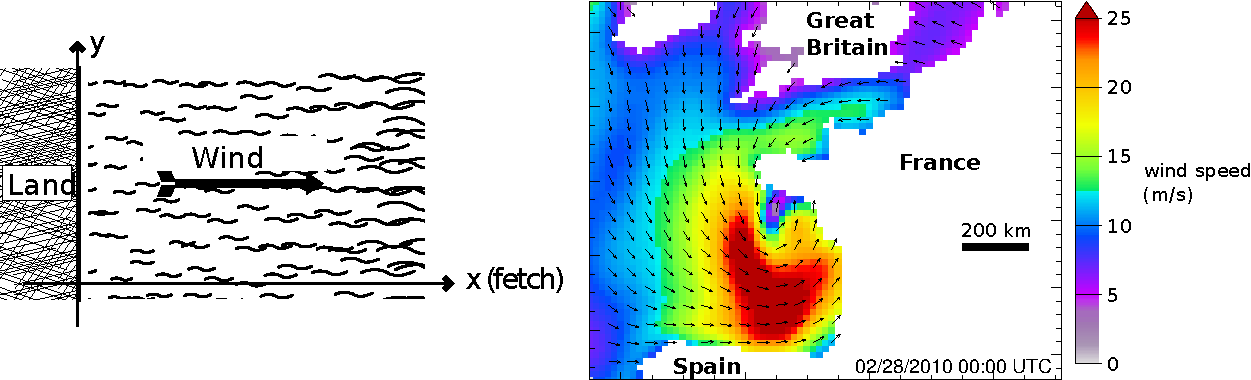
\includegraphics[width=0.8\textwidth]{FIGS_CH_FETCH/fetch_schematic.pdf}}
  \caption{Definition of fetch.}{Left: idealized conditions, Right: a real case 
  corresponding to the 2010 Xynthia Storm, which caused severe coastal flooding in France: the wind speed varies rapidly 
  in space and time, making it very difficult to define a fetch for an equivalent constant wind. The Xynthia storm crossed the bay of Biscay 
  in 6 hours going to the North-East, as a result the waves had little time to develop.} \label{fig:fetch}
\end{figure}
%%%%%%%%%%%%%%%%%%%%%%%%%%%%%%%%%%%%%%%%%%%%%%%%%%%%%%%%%%%%%%%%%%%%%%%%
In the open ocean, $X$ is not easy to define precisely, and it can 
be taken as an order of magnitude, in relation with a representative wind speed $U_{10}$: the region where winds are very high is typically smaller than the
region where winds are lower, so that the choice of the wind speed will modify the fetch. 

The use of $U_{10}$ as the variable representing the strength of the wind is also fairly arbitrary. 
Many studies have debated the possibly better choice of the friction velocity in the air, 
 $u_{\star a}=(\tau_a / \rho_a)^{1/2}$. %unfortunately, the scatter of wave parameters as a function  $u_{\star a}$ is almost as large as  when $U_{10}$ is used. 
Since wind speed measurements are usually converted to $U_{10}$ and more often measured than  $u_{\star a}$, it turns out to 
be more practical to use $U_{10}$. 
% NB: Analysis of Xynthia waves would be a good M1 / M2 topic. 

% LOGIC PROBLEM BELOW ... CF MARINE

In the most simple case, represented in figure \ref{fig:fetch}, 
a uniform wind speed blowing perpendicularly offshore from a straight shoreline. In such conditions 
Sverdrup and Munk found that the dimensionless wave energy  
\begin{equation}E^\star=E g^2 / U_{10}^4
\end{equation} and wave period
\begin{equation}
f_p^\star=f_p U_{10} / g
\end{equation}
%$\widetilde{E} = H^2 g^2 / U_{10}^4,$ 
% define E ...
 where $E$ and $f_p$ are the free surface elevation variance 
and the frequency of the elevation spectral peak, respectively, varies as a function of the dimensionless fetch
\begin{equation} X^\star=X g /
U_{10}^2 \end{equation} and duration
\begin{equation}
t^\star=t g/U_{10}.
\end{equation}
%A similar result was obtained for the  dimensionless wave period.  $1/f_p^\star= Tg / U_{10}$. 
Figure
(\ref{growthSHOWEX}) shows values measured at a time  $t^\star >
10^5$, for which the sea state does not depend on duration anymore. The figure also includes a comparison with 
the average measured values during other experiments \cite{Kahma&Calkoen1992,Kahma1981}.
%%%%%%%%%%%%%%%%%%%%%%%%%%%%%%%%%%%%%%%%%%%%%%%%%%%%%%%%%%%%%%%%%%%%%%%%
\begin{figure}[htb]
\centerline{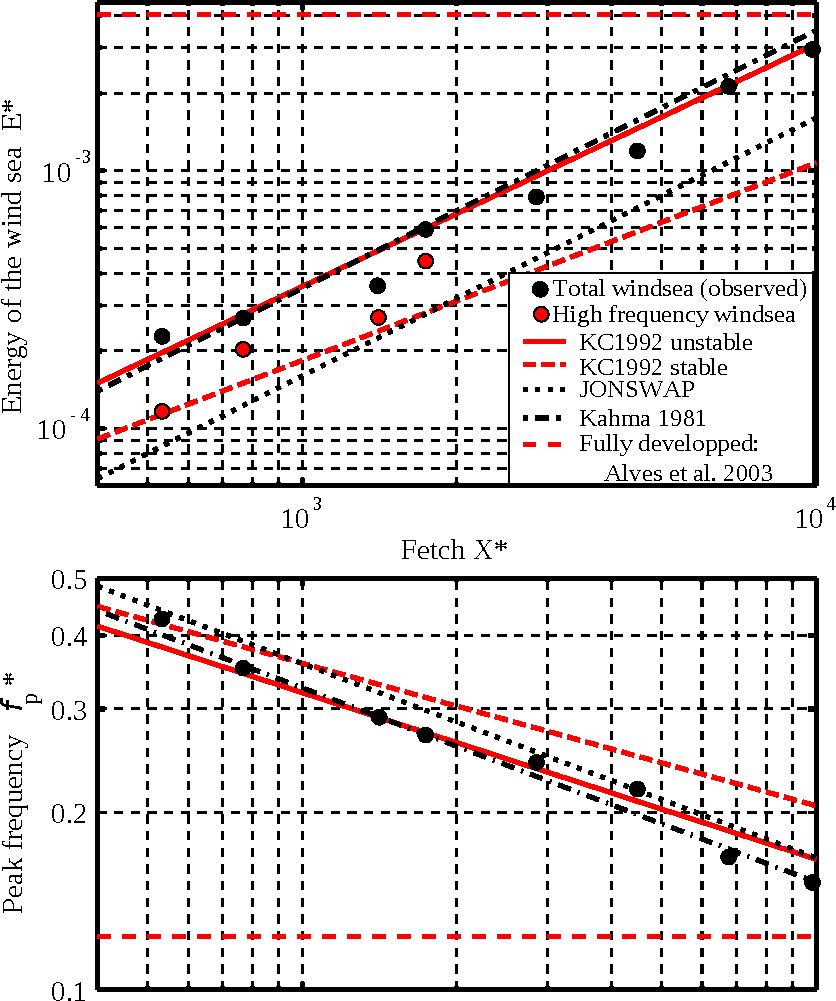
\includegraphics[width=0.6\textwidth]{FIGS_CH_FETCH/wave_growthSHOWEX_en.pdf}}
  \caption{Growth of waves with fetch, measured during  the Shoaling Waves Experiment (SHOWEX) in 1999, 
off the North Carolina Outer Banks. The wind is blowing at an angle of 70 degrees relative 
to the shoreline, which generates a double peak in the wind sea for the shortest fetches. Very close to shore, the 
high frequency part of the wind sea (in red) is in the wind direction, while an 'alongshore wind sea' (in black) grows to lower frequencies, 
in the direction of the largest available fetch. For comparison, several empirical growth curves 
are superimposed, as given by Kahma et Calkoen (1992), and Kahma (1981) from other datasets, and 
the expected 'full development' proposed by \cite{Pierson&Moskowitz1964}, as re-analysed by \cite{Alves&Banner2003}. \label{growthSHOWEX}}
\end{figure}
%%%%%%%%%%%%%%%%%%%%%%%%%%%%%%%%%%%%%%%%%%%%%%%%%%%%%%%%%%%%%%%%%%%%%%%%

%\subsection{La loi de Toba}
%Alors que les observations de $E^\star$ et $f_p^\star$ peuvent varier d'un
%facteur 2 pour une valeur de $X^\star$, Toba

\subsection{Full development and wave age}
For large fetches, the wave energy and peak frequency appear to tend to an asymptotic limit. 
This is very difficult to verify for moderate to strong winds, because the required non-dimensional fetch 
$X^\star_0=2.2 \times 10^4$ is already 220 km for $U_{10}= 10$ m/s. 
In practice we have very few observations for steady and uniform winds over a non-dimensional fetch larger than  $X^\star
> 10^4$. In search of such conditions, Pierson and Moskowitz
(1964\nocite{Pierson&Moskowitz1964}) have carefully selected 
55 records obtained from weather ships. From these measurements they estimated the asymptotic values  
\begin{equation}
E^\star=0.00402
 \end{equation}
 and
\begin{equation}
f_p^\star=0.123.
\end{equation}

The stage of development of waves, limited by fetch or duration, can be defined 
by the wave age, 
\begin{equation}
 A=C_p / U_{10}
\end{equation} where $C_p=2 \pi f_p/k_p$ is the phase speed at the peak of the spectrum. 
This parameter can be used to separate the wind sea, which is generated by the local wind and corresponds to 
young waves, with ages less than 1.2, and swell, for which the local wind has almost no effect, 
and which corresponds to older waves, with ages larger than 1.2. \cite{Donelan&al.1992} showed that 
the wave growth stops or at least becomes very slow, when  $C_p / U_{10} > 1.2$, confirming the analyses of \cite{Pierson&Moskowitz1964}. 
This means that, for a fully developped sea state, the dominant waves are propagating 20\% faster than the wind speed. 

\subsection{Fetch limitation}
The region where the wind is faster than a given value of  $U_{10}$ is always finite. This can limit the wave energy and peak frequency to a value 
lower than what would happen in a larger region. A practical important problem is the actual value reached by the wave height and peak period is 
such a limited area. With the non-dimensional fetch at full development $ X^\star_0 \simeq 2.2 \times 10^4$, all measurements lead to empirical 
wave growth formulae that are close to
\begin{eqnarray}
   C_p/U_{10}  & \simeq &  1.2  \left(\min
   \left\{\frac{X^\star}{X^\star_0},1\right\}\right)^{0.33},\label{ageElf}\\
   H_s  & \simeq &  0.26 \frac{U_{10}^2}{g}\left(\min
   \left\{\frac{X^\star}{X^\star_0},1\right\}\right)^{0.5}.\label{Hs_fetch}
\end{eqnarray}
We remember that in deep water, 
\begin{equation}
T_p = \frac{2 \pi C_p}{g},
\end{equation}
which yields $T_p$ from $C_p$.

The empirical growth laws (\ref{ageElf})--(\ref{Hs_fetch}) are a practical set of equations to 
obtain a quick estimate of the order of magnitude of the sea state, with heights within a factor two of the measurements, as shown in figure \ref{growthSHOWEX}.  
Many variants of thes equations have been published, with numerical values of the proportionality coefficients that may vary by a factor 2 \citep{Kahma&Calkoen1992}.
These differences are probably due, among other things, to the variations of the 
wind which is never exactly stationary nor uniform, and not exactly perpendicular to the shoreline... which is itself never quite straight and infinitely 
long. A careful analysis by \cite{Young1998} reveals that some of the differences between the different datasets may be due to differences between the air and sea 
temperature, which modify the properties of the turbulence in the atmospheric boundary layer. The details of how that impacts the wave growth is still 
not understood. One possible factor is that the wind tends to be less regular (more gusty) in unstable conditions when the water is warmer than the air. It is 
well understood that this increased gustiness can lead to higher waves for mature waves with $X^\star
> 10^4$, as shown by \cite{Abdalla&Cavaleri2002}. 
%%%%%%%%%%%%%%%%%%%%%%%%%%%%%%%%%%%%%%%%%%%%%%%%%%%%%%%%%%%%%%%%%%%%%%%%%%%%%%%%
\begin{figure}[htb]
\centerline{\includegraphics[width=\textwidth]{FIGS_CH_FETCH/fetch_time_lim_contours.pdf}}
 \caption{Estimation of significant wave height ($H_s$, contours) as a function of fetch and duration for the idealized case of an infinitely long coast 
with a wind blowing perpendicularly offshore at a speed $U_{10}=20$~m/s. In the left panel the estimate is given by a numerical integration of 
the wave action equation, defined in the next 
chapter, using parametrizations for the wind-wave growth and dissipation from \cite{Rascle&Ardhuin2013} and non-linear wave-wave interactions 
from \cite{Hasselmann&al.1985b} using the WAVEWATCH III model, with a third order numerical scheme \cite{Tolman1995b}. The right panel combines eq. 
(\ref{Hs_fetch}) and eq. (\ref{eq:time_limit}). Both give the time-limited growth for large fetches and the 
fetch-limited growth for large durations, with no more growth when waves reach full development at $H_s \simeq 10.8$~m. The dashed line is the same in both panels. 
In the left panel, the model gives a slow increase of the wave height even after the time limitation has been exceeded: this is because the infinitely long shoreline allows 
the growth of very oblique components that travel very long distances alongshore. That effect is not represented in the empirical formula of eq. (\ref{eq:time_limit}). 
It is a well documented effect for oblique fetches when the wind is not perpendicular to the coast \citep{Ardhuin&al.2007}, but there is no description of 
this phenomenon for winds perpendicular to shore. \label{fetch_time}}
\end{figure}
%%%%%%%%%%%%%%%%%%%%%%%%%%%%%%%%%%%%%%%%%%%%%%%%%%%%%%%%%%%%%%%%%%%%%%%%%%%%%%%%%

\subsection{Time limitation}
If the wind has started to blow only a short time ago, with $t^\star < 10^5$, the sea state parameters 
can be estimated, replacing $X^\star$ with
\begin{equation}
X^\prime = (t^\star/70)^{1.3}. \label{eq:time_limit}
\end{equation} 

\subsection{Double limitation}
In practice, the sea state is often limited by both time and fetch. 
The sea state parameters are then given the lowest of the two values for $H_s$ and $C_p/U_{10}$ 
between the one obtained with $X^\star$ and the one obtained with $X^\prime$ \citep[see][]{CERC1977}. 
For an alternative estimation, one may read \cite{Hwang&Wang2004}. This double limitation is illustrated by figure \ref{fetch_time}.



\section{Swell}
So far we have only discussed the wind sea, which is related to the local wind. However,  
the sea state often contains an important swell contribution, which are waves radiating away from their area of generation. We can define swells as the waves for which the source 
of energy from the wind is zero or negative, in practice it corresponds to waves travelling at a phase speed $C$ faster than the wind speed $U_{10}$, or at angle relative 
to the wind $\theta_w - \theta_u$ such that $U \cos(\theta_w-\theta_u) < C$. This definition is often extended to allow the peak of a fully developped wind sea, which can 
travel at a phase speed of 1.2 $U_{10}$, to be classified as wind sea. This extension is equivalent to adding the source of energy from the nonlinear wave-wave interactions to 
the source of energy from the wind in order to separate wind seas and swell. Because the wind is neither steady nor uniform the boundary between wind sea and swell is rather 
fuzzy. 

Swells is most important in large oceanic basins, in particular near their eastern boundary as the dominant winds generally blow from west to east where it can account for 
more than 90\% of the wave energy \citep[e.g.][]{Chen&al.2002}. The swell is the part of the sea state that cannot be amplified 
by the local wind because they are too fast, or travel at an angle too oblique to the local wind. 
This swell can be composed of distinct individual swells, travelling in different directions and 
with different dominant frequencies, these swells are the result of the evolution of 
wind seas that propagate out of their generation area. 
Swells, when they exist, generally have longer periods than the wind sea because short waves are rapidly dissipated away from their generation area. They are thus the result of storm conditions, with winds strong enough to generate large period waves, as given by eq. \ref{ageElf}. The stronger and larger the storm, the longer the swell period. 
%%%%%%%%%%%%%%%%%%%%%%%%%%%%%%%%%%%%%%%%%%%%%%%%%%%%%%%%%%%%%%%%%%%%%%%%%%%%%%%%
\begin{figure}[htb]
\centerline{\includegraphics[width=0.8\textwidth]{FIGS_CH_FETCH/SWAO_nature_figS1_en.pdf}}
 \caption{Example of the evolution of wave energy and mean direction as a function of frequency
and time, over one month, measured at the Christmas Island buoy (Kiritimati, Kiribati), 
in the middle of the Pacific. Contour values equally spaced between 
0.1 and 1.4 correspond to the logarithm of the spectral density $E(f)$, colors 
correspond to the mean direction for each frequency. The oblique dashed line 
from 15 July at 0.05 Hz to 18 July at 0.8 Hz correspond to eq. (\ref{prev lin1}) 
with a distance $R \alpha= 6100$~km between storm and observation point. 
The intersection between this line and the axis $f=0$ gives the date of the storm: July 9, 
when a severe storm was indeed present south of New Zeland. \citep[taken from][]{Collard&al.2009}.\label{ridges}}
\end{figure}
%%%%%%%%%%%%%%%%%%%%%%%%%%%%%%%%%%%%%%%%%%%%%%%%%%%%%%%%%%%%%%%%%%%%%%%%%%%%%%%%%

Modern swell studies started during the colonial war between France and Morocco in 1906. In the absence of safe harbors on the atlantic coast of Morocco, the disembarkment of troops and supplies used small shuttle boats that could be destroyed by heavy swells. Such an event made the harbor of Casablanca unavailable for several months. 
Swell forecasting for Morocco became a an important matter, and the first method was based on 
the propagation of swells from the mid-atlantic Azores Islands where visual observations were made several times a day \citep{Gain1918}. 
This method was used in the swell forecasting office of Casablanca in the early 1920s \citep{Montagne1922}, where the first modern numerical wave models were invented \citep{Gelci&al.1957}. 

In the Pacific or Indian oceans, it is very common to find at the same time and place 
 several swells coming from distinct storms (e.g. Figure \ref{fig:Hawaii_spectrum}), that may have happened 10,000 km away and a week before \citep{Darbyshire1957, Munk&al.1963}. 
Owing to the large distances travelled by swells, the sphericity of the Earth must be taken into account. The re-derivation of linear wave theory in that case 
shows that the swell that propagated along a straight line on a flat ocean, now travel on the shortest path on the sphere, which are the great circles:  
the circles that have their centers at the center of the Earth, such as the meridians. 

The height and period of swells depend on the height and period of waves in the strom, and the propagation distance outside of the storm. Storms generate waves with a wide range of periods up to about 1.2 times the peak period $T_p$. This mixture of waves `disperses', and because the group speed $C_g=g T/(4 \pi)$  in deep water, is a function of the period $T$, 
the largest period swell arrive first, followed by shorter swells. 
At very large distances, the storm from which the swell radiates can be considered a point in 
space and time. The evolution of the swell peak period at a remote observation position follows, 
\begin{equation}
T_{\mathrm{ps}} (t) = \frac{4\pi R \alpha }{g(t-t_0)},
\label{prev lin1}
\end{equation}
where $R$ is the Earth radius, $t_0$ is the time of the storm, and $\alpha$ is the spherical distance, i.e. the angle -- in radians -- at the center of the Earth between the storm and the observation point. This relationship very well verified, as shown in figure \ref{ridges}.


Swell heights decrease during propagation due 
to the dispersion from the source, and also due to dissipation. Dispersion is the main effect for swell periods larger than 12 s, 
and corresponds to a stretching of the wave fronts in the direction perpendicular to propagation, just like circles becoming larger 
away from a stone dropped in a pond. There is also a stretching of the wave train in the propagation direction due to the different group 
speeds, the longer wave periods contribute to a longer wave train away from the storm, while the shorter wave periods are travelling 
slower behind. This spatial spreading of the swell field is illustrated with numerical model results in 
figure \ref{reconst_champ}, taken from \cite{Delpey&al.2010}. 
%%%%%%%%%%%%%%%%%%%%%%%%%%%%%%%%%%%%%%%%%%%%%%%%%%%%%%%%%%%%%%%%%%%%%%%%%%%%%%%%%%%%%%
\begin{figure}[htb]
\centerline{\includegraphics[width=0.6\textwidth]{FIGS_CH_FETCH/partition_globes_small.pdf}}
 \caption{Swell radiated from a storm.}{(a,b,c) peak periods of the swell $T_{ps}$ and (d,e,f) significant swell heights  $H_{ss}$ 
from a realistic numerical model of the storm of February 24, 2004, centered at (160$^{\circ}$ E, 42$^{\circ}$ N). 
The maps correspond to  February 27th (top) 
 March 1st (middle) and March 6th (bas) at 00h UTC, which is 3, 6 and 9 days after the storm \citep[reproduced from][]{Delpey&al.2010}.\label{reconst_champ} }
\end{figure}
%%%%%%%%%%%%%%%%%%%%%%%%%%%%%%%%%%%%%%%%%%%%%%%%%%%%%%%%%%%%%%%%%%%%%%%%%%%%%%%%%%%%%%
Neglecting dissipation effects, and for distances of the order of 4000 km or more from the storm center, 
the decrease in swell height following the peak in space and time is given by 
\begin{equation}
H_{ss} (\alpha) = H_{ss} (\alpha_0)  \sqrt{\frac{\alpha_0  \sin \alpha_0}{\alpha \sin \alpha}}.
\label{swell_asymptote}
\end{equation}
In practice, the height is further reduced by islands and continents 
where it breaks and dissipates on the shore. Dissipation in deep water is locally weak but can add up to a significant effect 
over long propagation distances \citep{Ardhuin&al.2009b}. Even with these effects, it is possible to record swells coming from the 
antipodes \citep[e.g.][]{Munk&al.1963}. 
 

\section{Frequency spectra}
\subsection{The early days}
The first measurements of wave spectra from time series were performed in 1944, as part of the efforts of Group W at the British Admiralty, 
after the amphibious assault on Normandy  \citep[][]{Barber&al.1946,Ursell1999}. These records, and the many others that followed, 
revealed that for frequencies above the spectral peak, the decrease in energy takes always the same form. \cite{Phillips1958}
 introduced the idea of an  equilibrium region for
$f>f_p$, and proposed that gravity was the only determining factor for that part of the spectrum which was controlled by wave breaking.  
Dimensional analysis leads to the shape 
\begin{equation}
   E(\sigma)=\alpha_P g^2 \sigma^{-5} \quad \mathrm{soit} \quad E(f)=\alpha_P \left(2\pi\right)^{-4} g^2 f^{-5},
\end{equation}
where $\alpha_P\approx 0.008$ is now called Phillips' constant. The non-dimensional energy $E(\sigma) \sigma^{5}/g^2$ is constant
in this model: the surface is thus fractal without any particular scale. In other words, these waves are self-similar and have all the same 
shape, whether they are large or small. 
%%%%%%%%%%%%%%%%%%%%%%%%%%%%%%%%%%%%%%%%%%%%%%%%%%%%%%%%%%%%%%%%%%%%%%%%%%%%%%%%%%%%%%%%%%%%
\begin{figure}[!hbt]
\centerline{\includegraphics[width=\textwidth]{FIGS_CH_FETCH/overshoot_JONSWAP_SHOWEX.pdf}}
  \caption{Evolution of the wave spectrum with fetch.}{(a) measured spectra on September 15, 1968 at 11h
  during JONSWAP, with, inset, the proposed parameters for the JONSWAP spectrum. Numbers indicate the fetch in kilometers. (b) spectra measured on November 3rd, 1999, averaged from 13h to 17h during SHOWEX, 
using Datawell Mark III waverider buoys. 
Note that the scale is logarithmic. In the SHOWEX case, the wind speed is 10 m/s, 20 degrees from the shore-normal. The peak around $f=0.1$~Hz
  corresponds to swell arriving from the Atlantic, against the wind. The instrument at the shortest fetch 
reveals two peaks in the wind sea, at 0.25 and 0.45 Hz. The analysis of wave directions, not shown here, show that the first peak is propagating 
alongshore, and the second is in the 
wind direction. The existence of the first peak is due to the oblique 20$^\circ$ angle between the wind and the shore-normal.}
\label{fig_overshoot}
\end{figure}
%%%%%%%%%%%%%%%%%%%%%%%%%%%%%%%%%%%%%%%%%%%%%%%%%%%%%%%%%%%%%%%%%%%%%%%%%%%%%%%%%%%%%%%%%%%%
These ideas were also developed by \cite{Kitaigorodskii1962}, and  led \cite{Pierson&Moskowitz1964} to propose an empirical 
shape for the full spectrum, based on fully developed sea states, 
\begin{equation}
   E(f)=E_{PM}(f)=\alpha_{P} g^2 \left(2\pi\right)^{-4} f^{-5} \exp\left[-\frac{5}{4}
   \left(\frac{f}{f_p}\right)^{-4}\right].
\end{equation}
At short fetch, it was soon realized that spectral shapes could be significantly different. 
The peak is particularly narrower for young sea states. Also, the values of the spectral density $E(f)$ for a given frequency $f$
can be larger than those found for old seas: this overshoot of the spectral peak was first discussed by \cite{Barnett&Sutherland1968}, 
and further investigated during the 1968-1969 Joint North
Sea Wave Project \citep[JONSWAP, see][]{JONSWAP},
figure \ref{fig_overshoot}).

Based on these observations, a `peak enhancement' was added to the Pierson-Moskowitz (PM) shape, 
\begin{equation}
   E(f)=E_{PM}(f) \gamma^{\exp\left[\frac{-\left(f-f_p\right)^2}{2 \sigma_{A/B}^2
   f_p^2}\right]}. \label{SpectreJONSWAP}
\end{equation}
This may look a bit complex, but each parameter plays a fairly clear role, illustrated in figure \ref{fig_overshoot}.a. 
$\gamma \simeq 3.3$ is the `peak enhancement-factor', if equal to 1 then the spectrum is a PM spectrum,  $\sigma_{A/B}$ 
is the relative width over which this enhancement applies. It was found that  $\sigma_{A} \simeq 0.07$
if $f<f_p$ and $\sigma_{B} \simeq 0.09$ otherwise. Using (\ref{SpectreJONSWAP}) and (\ref{ageElf}) one can estimate 
 $C_p$ and $f_p=g/(C_p 2 \pi)$ as a function of the wind speed. This gives the average spectral shape measured 
in the North Sea during JONSWAP. 

\subsection{The modern era}
More recent obvservations, starting with \cite{Toba1973}, have shown that, at frequencies between 
$f_p$ and $3 f_p$, the spectrum was not following  $f^{-5}$ but  $f^{-4}$. This shape can be obtained 
by including the wind speed or friction velocity in the dimensional analysis, it also corresponds to a 
constant flux of energy towards high frequencies due to the non-linear wave-wave interactions. In passing, we can see 
that it is always easy to find a theory for anything after the observations have been made. 
This $f^{-4}$ decrease near the spectral peak is particularly well verified by the wave gauge array data of \cite{Donelan&al.1985}, 
which was one of the first clean measurements of the spectrum in both frequency and directions. \cite{Donelan&al.1985} also proposed 
a spectral shape that reconciles the peak enhancement of the JONSWAP data with the mature wave spectral shape of \cite{Pierson&Moskowitz1964}. 
The adjustment given here in eq. (\ref{ageElf}) is an adaptation by \cite{Elfouhaily&al.1997}, giving the proper asymptotes for wave energies and periods. 
Further analysis by \cite{Long&Resio2007} have shown that there is in general a transition from  $f^{-4}$ at frequencies above the windsea peak  to  $f^{-5}$ at higher frequencies, and the 
frequency where this transition occurs appears to be a function of wave age. 

This discussion of the detailed shape of the wave spectrum at frequencies beyond $2 f_p$ may sound unimportant because it affects a very small fraction of the wave energy.
However, that part of the spectrum supports most of the energy flux from the wind to the waves, and thus defines the roughness of the sea, and thus the growth rate due to the wind for
the entire spectrum. Also, these short waves dominate the surface slopes, which strongly affect ocean remotely sensed properties such as sea level, surface salinity and wind speed 
and direction. Measurements of the sun reflection by the ocean performed by \cite{Cox&Munk1954} give a very good estimate of the mean square slope (mss),
\begin{equation}
   \mathrm{mss}=\int \left(k_x^2+ k_y^2 \right) E(k_x,k_y) {\mathrm d} k_x {\mathrm d} k_y \simeq
   \int \frac{(2 \pi f)^4}{g^2} E(f) {\mathrm d} f, \label{eq:mss_int}
\end{equation}
where the second equality uses the linear wave approximation. In order to have a finite value of the mss, 
$E(f)$ must decrease faster than $f^{-5}$ towards the high frequencies. 
\cite{Elfouhaily&al.1997} and \cite{Kudryavtsev&al.1999} have used this argument and detailed remote sensing data to propose a parametric 
shape of the wave spectrum that is a function of wind speed and wave age, and includes a strong decrease for  $k> 10 k_p$, 
taking also into account the effect of surface tension \citep[see also][]{Dulov&Kosnik2009,Yurovskaya&al.2013}.
A few proposed parametric spectral shapes for gravity waves are compared in figure \ref{spectra_comp}. In practice there is a very strong variability 
of the observed specta around these average shapes due to spatial and temporal variations in wind speed and direction.
It should also be noted that for $f > 4 f_p$ there can be a dominant contribution of non-linearities, as revealed in stereo-video imagery (see figure \ref{fig:kxky} in 
the preceding chapter).

%%%%%%%%%%%%%%%%%%%%%%%%%%%%%%%%%%%%%%%%%%%%%%
\begin{figure}[htb]
\centerline{\includegraphics[width=\textwidth]{FIGS_CH_FETCH/Spec_comp50km_linlog_en.pdf}}
%\vspace{3.64in}
  \caption{Example of proposed parametric wave spectrum shapes, for $U_{10}=10$~m~s$^{-1}$ et $X=50$~km. Left: using a linear scale and 
right, the same spectra with a logarithmic scale. The slope of the curves in log scale gives the power  $n$ of the 
  dependance  $E(f) \propto f^{-n}$. Note the transition from
  $n=4$ for $f< 2 f_p$ to $n>5$ at higher frequencies, broadly consistent with the analysis of \cite{Long&Resio2007}. 
  We have extended here the \cite{Donelan&al.1985} spectrum beyond its range of validity, namely for $f>3 f_p$, in order 
to better visualize its  $f^{-4}$ decay.}
\label{spectra_comp}
\end{figure}
%%%%%%%%%%%%%%%%%%%%%%%%%%%%%%%%%%%%%%%%%%%%%%%

\section{Directional spectra} 
\subsection{Early parameterizations}
The distribution of wave energy as a function of directions, is still very much debated because of the 
difficulty of measuring details of that distribution. Indeed, a wave buoy only measured 5 parameters for each direction \citep[e.g.][]{Kuik&al.1988}, and even 
ADCP systems are generally too noisy to go beyond the mean direction and possibly spreading at each frequency \citep{Herbers&Lentz2010}. 
There are, however, important constraints on the high frequency directional distribution, with a surface slope variance which is almost the same in the downwind and 
crosswind directions. 

The frequency-direction spectrum $E(f,\theta)$ is often decomposed into a frequency spectrum and a 
normalized directional distribution 
\begin{equation}
   E(f,\theta)=E(f)S(f,\theta)
\end{equation}
with the normalization
\begin{equation}
   \int_0^{2\pi} S(f,\theta) {\mathrm d}\theta=1.
\end{equation}

The first parameterizations of $S(f,\theta)$ used the fact that $S$ is a periodic function 
and that buoys can provide the first terms in its Fourier decomposition, 
\begin{equation}
S(f,\theta)=\frac{1}{2\pi} + a_1(f) \cos(\theta) + b_1(f) \sin(\theta) + ... 
\end{equation}
This was soon abandonned because $S$ can be negative for some directions if the series is truncated. \cite{Longuet-Higgins&al.1963} proposed 
another distribution that is always positive  
\begin{equation}
   S(f,\theta)=\cos^{2s}\left((\theta-\theta_m)/2\right),
\end{equation}
which is symetric about the direction of the maximum $\theta_m$, and narrower for larger $s$. This shape is still widely used, 
although $s$ cannot be readily measured, whereas the directional spreading  $\sigma_\theta$ (defined in 
chapter \ref{ch2}), is directly related to co-spectra of measured displacements or velocities. 
The width of the directional spectrum is generally minimum at the spectral peak, and increases towards both higher 
and lower frequencies.  The mean direction, even for the wind sea, can differ significantly from the wind direction, 
in particular at short fetch (see figure
\ref{fig_SHOWEX_dir}).

Among other proposed forms, the one by \cite{Donelan&al.1985} is based on theoretical solutions for non-linear wave groups,
\begin{equation}
   S(f,\theta) \propto \frac{1}{\cosh^2\left[\beta \left(\theta-\theta_m\right)\right]}
\end{equation}
and observations suggest $\beta = 2.44 (f/0.95 f_p)^{1.3}$ for $0.56<f/f_p < 0.95$ and
$\beta = 2.44 (f/0.95 f_p)^{-1.3}$ for $0.95<f/f_p < 1.6$. 
%From stereo-photographs, which cannot 
%resolve a 180 degree ambiguity in the propagation direction, 
%\cite{Banner1990} proposed $\beta =
%10^{-0.4+0.8393 \exp\left[-0.567 \ln\left(f/f_p\right)^2\right]}$
%for $f/f_p > 1.6$. 
That particular shape has been used for the estimation of the wind direction from HF radar data because they have non-zero values 
in the direction opposite to the wind direction, consistent with radar data. Unfortunately they still have a single maximum. 
%%%%%%%%%%%%%%%%%%%%%%%%%%%%%%%%%%%%%%%%%%%%%%%%%%%%%%%%%%%%%%%%%
\begin{figure}[htb]
\centerline{\includegraphics[width=0.7\textwidth]{FIGS_CH_FETCH/bimodal_en.pdf}}
%\vspace{3.64in}
  \caption{Average spectral distribution measured in Currituck sound for $U_{10} > 7$~m~s$^{-1}$ (From Long and Resio 2007).}
\label{bimodal}
\end{figure}
%%%%%%%%%%%%%%%%%%%%%%%%%%%%%%%%%%%%%%%%%%%%%%%%%%%%%%%%%%%%%%%%%

\subsection{Bimodality of the directional spectrum}
Indeed, detailed observations using arrays \citep{Young&al.1995,Long&Resio2007} or surface mapping systems with radar or optical imagery 
\citep{Hwang&al.2000b,Romero&Melville2010,Leckler&al.2015} have clearly revealed that for  $f > f_p$ the wind sea generally has two peaks 
on either side of the wind direction, as shown in figure 
\ref{fig:kxky} and \ref{bimodal}. Such a distribution is called bimodal. For frequencies $f>3f_p$ these peaks are 60 to 80 degrees 
away from the wind direction, at least for young waves ($C_p/U_{10} < 1/3$). 
There is no simple parametric form for these bimodal spectra, and their general shape for more mature waves is not established. 
Also, numerical models have a hard time reproducing clearly bimodal spectra, as discussed by \cite{Alves&Banner2003}. In general, for the dominant waves, we only have a good knowledge of the mean direction and directional spreading. 
One example of these two parameters is shown in figure \ref{fig_SHOWEX_dir}).
%%%%%%%%%%%%%%%%%%%%%%%%%%%%%%%%%%%%%%%%%%%%%%%%%%%%%%%%%%%%%%%%%
\begin{figure}[htb]
\centerline{\includegraphics[width=0.7\textwidth]{FIGS_CH_FETCH/showex_spectra_dir.pdf}}
%\vspace{3.64in}
  \caption{Example of measured directional parameters}{Measurements during SHOWEX on November 3rd 2003, in presence of a 1 m swell opposing 
the wind sea. The wind direction is from 270$^\circ$ and the shoreline faces 70$^\circ$. 
The different wave systems are clearly separated by a local maximum of the directional spreading 
  $\sigma_\theta$}.
\label{fig_SHOWEX_dir}
\end{figure}
%%%%%%%%%%%%%%%%%%%%%%%%%%%%%%%%%%%%%%%%%%%%%%%%%%%%%%%%%%%%%%%%%

As a result, applications that require a detailed knowledge of the directional spectrum, such as the interpretation of double-frequency 
acoustic and seismic noise, have to deal with large uncertainties. In fact, underwater acoustic data is one important source 
of measurements that can be used to better constrain our knowledge of the directional wave spectrum \citep{Tyler&al.1974}. This 
source of data is now  better understood \citep{Ardhuin&al.2013} and is still  being explored  \citep{Farrell&Munk2008,Duennebier&al.2012,Peureux&Ardhuin2016}. 
This aspect is detailed in Part 3. 

At high frequencies, remote sensing using HF \citep[e.g.][]{Kirincich2016} or microwave radars can also constrain the directional distribution, and specific spectral 
shape parameterizations have been proposed by, for example, \citep{Elfouhaily&al.1997} and \citep{Kudryavtsev&al.2003a}
 to provide  wave spectra  consistent with radar observations. With more data available now in new microwave bands 
such as L band \citep[e.g.][]{Yueh&al.2013}, and detailed wave shape measurements from stereo-video and polarimetric systems, 
there will certainly be improvements in the coming years. 



\subsection{Swell spectra}
The spectrum of a swell system is simply a wind sea spectrum that has dispersed 
and dissipated. Due to the dispersion, it is much more narrow than a wind sea spectrum, and this narrowness increases with the 
distance from the storm. This narrow peak may be parameterized by a Gaussian, with a frequency bandwidth that is  proportional
to the size of the storm and inversely proportional to the spherical distance $\alpha$  from the storm \citep{Collard&al.2009}. 
The directional width is also increased by the storm size and reduced by the distance, with one important difference due to the Earth 
sphericity. Indeed, beyond one quarter of the Earth circumference, the directional width increases 
if no land has blocked the swell, and is proportional to  $1/\sin (\alpha)$. Hence, the 
decrease in wave height given by eq. (\ref{swell_asymptote}) 
corresponds to a narrowing of the spectrum, not to a reduction of the spectral density. Indeed, 
in absence of disspation, for deep water and without current, the 
spectral densities  $E(f,\theta)$ are conserved during propagation. Namely 
$E(\lambda_0,\phi_0,t_0,f,\theta_0)=E(\lambda',\phi',t',f,\theta')$, where the point of coordinates  $(\lambda,\phi,t)$ is on the same 
great circle as the point  $(\lambda_0,\phi_0,t_0)$, and such that the azimuth of the great circle changes from $\theta_0$ to $\theta$. 

\section{Summary}
\subsection{Important parameters}
 We have seen that the most important factor that control the wind sea are 
\begin{itemize}
  \item the wind speed $U_{10}$
  \item the fetch  $X$
  \item the duration $t$ over which the wind has been blowing.
 \item The depth $D$, which was not discussed here. The reader may follow \cite{Young1999}. 
 \end{itemize}
Other parameters also have a quantitative effect, 
\begin{itemize}
  \item the shape of the fetch area 
  \item the air-sea temperature difference $T_a - T_{\mathrm{sea}}$ and the larger gustiness when this difference is negative. 
  \item strong currents $C$ (if $U/C > 0.1$).
  \item rain. That latter factor is not well known and is probably not so important in general. 
\end{itemize}

The parameters of the first list have effects that are well understood. For the second list, the complex situations usually require 
the use of a numerical wave model in order to get a reliable estimate of the sea state parameter... but even in the models 
not all of these effects are well understood and thus not well parameterized in the models. The next chapter will present 
the main concepts used in numerical models for the evolution of waves in deep water. 

\subsection{Spectral shape}
Wave spectra estimated from measurements have a wide variety of shapes, in particular close to coastlines 
where the fetch limitation on wave growth gives mean direction that can vary with frequency. 
In the open ocean, multiple swell systems that come from remote storms are also often present.  (e.g. figure \ref{fig:Hawaii_spectrum}). 
The wind sea exhibits a clearly marked peak, where directional spreading has a local minimum, and a decrease of the spectral density $E(f)$ 
proportional to  $f^{-4}$ up to 2 to 3 times the wind sea peak frequency. For higher frequencies, the spectral density decreases like $f^{-5}$ or faster. 

In the directional distribution, there is always some energy in all directions, as revealed by high frequency radar data \citep[e.g.][]{Barrick&al.1974,Tyler&al.1974}
 but it can be very 
small. The wave spectrum generally has a marked bimodality at frequencies between 2 and at least 4 times the wind sea peak frequency, with two maxima on either side of the wind 
direction. This spectral shape is the result of different processes that, as we will see in the next chapter, can be represented in an equation for the evolution of the spectrum. 

\cleardoublepage
\chapter{Physics of spectral wave evolution: deep water}\label{ch_sourceterms}
The present chapter will give some general explanations on the physical processes that explain the observed sea state properties. It is now well understood that ocean waves derive most of their energy from the wind, and lose most of it to the ocean turbulence as they break. 
One particular motivation for understanding these physical processes is that beyond the wave spectrum, we may be able to quatify the fluxes of energy 
and momentum in and out of the wave field. 
Indeed, the generation of waves by the wind is thus associated to vertical fluxes of horizontal momentum and energy going 
from the wind to the wave field. This flux of momentum generally accounts for more than 70\% of the total momentum flux going 
from the atmosphere to the ocean, this total flux is usually called the wind stress. That air-sea momentum flux does not remain in the wave field, 
but rather it is lost by wave dissipation, mostly due to wave breaking, and ends up in the ocean currents. Most of this momentum 
loss happens at the same place where waves were generated: the wave field is thus largely 'transparent' to this momentum flux. However, a few percent of this 
momentum flux propagates away across ocean basins and is transformed into changes in sea level -- this is known as wave set up -- and currents on the beaches where waves break. 
These currents are the longshore currents. This transformation of wave momentum in the nearshore is the topic of chapter \ref{ch_littoral}. 
%%%%%%%%%%%%% figure
\begin{figure}[hbt]
\centerline{\includegraphics[width=0.7\textwidth]{FIGS_CH_SOURCETERMS/air_sea_fluxes_en.pdf}}
%\vspace{3.64in}
  \caption{Fluxes at the air-sea interface, at four phases of the wave profile: 1 windward slope, 2 crest, 3 leeward slope, 4 trough. 
The energy flux from the atmosphere to the ocean is the work of the stresses acting on the sea surface, 
   $\left[p \mathbf{n} + \tau\right] \bcdot (u,w)$, with $\mathbf{n}$ the unit normal vector pointing to the water side.
   As a result, if the air pressure is higher on the windward slope, then 
   $p_1 w_1 \left.\frac{\partial \zeta}{\partial x}\right|_1 > p_3 w_3 \left.\frac{\partial \zeta}{\partial x}\right|_3$
   and the pressure-related flux is positive towards the water side. 
   Likewise, if the shear stress  $\tau$ is opposed to the velocity vector (as here), the flux $\tau u$ induced by shear stresses is 
negative (i.e. energy goes from the water to the air). Similarly, the momentum flux is the average 
stress acting on the surface. Because of the surface slope, the vertical flux of horizontal momentum is the 
average of  $p {\partial \zeta}/{\partial x}$ plus the average of  $\tau_x$.} \label{airseaflux}
\end{figure}
%%%%%%%%%%%%% end of figure
%We shall see also in the next chapter that waves also carry some horizontal momentum, which, for monochromatic waves 
%of phase speed $C$ has a density per unit horizontal surface equal to $\rho_w g E/C$ and points in the wave propagation direction. 


Besides the generation or attenuation by the wind and dissipation associated to breaking, a third mechanism is very important for the 
evolution of the waves in deep water. It is the non-linear evolution of the waves which can be understood as a wave-wave scattering process: waves components 
exange energy and momentum, some components grow and others decay. In order to make things simple, we will now consider separately each of these three processes. 

\section{Generation of waves by the wind}
The fraction of the wave energy that is in the water is $(\rho_w -\rho_a)/\rho_w \simeq 99.9$\%. Hence the transfer energy from wind to waves 
involves a flux of energy through the sea surface. Because the surface is a material surface, this flux cannot happen by advection, it thus requires the 
work of stresses on the surface, either the tangential stresses $\tau$ or the normal stresses, i.e. the pressure $p$. In the case of tangential stresses, 
the work is the correlation of 
the along-surface shear stress with the along-surface orbital velocity. The work of normal stresses is the correlation of pressure times the velocity normal to the surface
 (see figure \ref{airseaflux}). A quantification of these energy fluxes thus require the identification of processes that produce pressure and shear stresses on the surface. 
The first hypotheses on wave generation followed the theory of hydrodynamic instabilities. The air flow over a water surface is a particular case of a sheared flow in a stratified 
medium that may lead to the Kelvin-Helmholtz (KH) instability. This may indeed be important for very high winds speeds \citep{Soloviev&al.2014}, but it cannot explain the 
initial growth of waves under moderate winds. In particular, KH theory predicts instabilities for an air-water interface for wind speeds above 6,5 m~s$^{-1}$ (Jeffreys 1925), 
but ripples already appear on the water surface for winds as low as  $U= 1,1$~m~s$^{-1}$
(Kahma et Donelan 1988\nocite{Kahma&Donelan1988}). 

This initial growth of ripples is rather well explained by the effect of turbulence in the air advected by the wind \cite{Phillips1957}. 
That process is very soon overtaken by the feedback caused by the wave-induced pressure oscillations in the air, as the airflow is modified by the presence of waves. 
 When waves travel slower than the wind projected in their propagation direction, the pressure is slightly higher on the windward face, typically of the order of a few Pascals,
and lower on the leeward side. 


We are thus going to generalize the Airy wave theory of chapter \ref{ch1b}. To simplify the calculations we will replace the wave amplitude $a$ by a complex amplitude  $Z_0=a \er^{\ir \Theta_0}$, so that the sea surface elevation is 
\begin{equation}
    \zeta= \overline{\zeta} + \Re \left[ Z_0 \mathrm{e}^{\mathrm{i}{\mathbf k}\bcdot{\mathbf x} - \sigma t} \right],\label{polzetain}
\end{equation}
where we recall that $ \Re$ represents the real part of a complex number. In a first approximation, we will assume that the atmospheric pressure is proportional but shifted in phase compared to the amplitude of the surface elevation, 
\begin{equation}
 p_a= \overline{p}_a + \rho_w g \Re \left[ \left( \alpha + {\mathrm i}\beta\right)   Z_0 \mathrm{e}^{\mathrm{i}{\mathbf k}\bcdot{\mathbf x} - \sigma t} \right], \label{wave_induced_pa}
\end{equation}
where $\alpha$ represents the in-phase oscillations and $\beta$ the oscillations in quadrature. 

Here we will take $\alpha=0$ for simplicity as we shall see that it is not important for wind-wave growth. 
When $\beta \ll 1$, we assume that the air pressure only makes a small $O(\beta)$ correction to the solution we found in  chapter \ref{ch1b}. 
Bernoulli's eq. (\ref{p_all}) at the surface now has a forcing term from the atmospheric pressure. For propagating waves we can neglect $\gamma(t)$, giving, 
\begin{equation}
    \frac{\partial \phi}{\partial t} \simeq 
       - g \zeta - \overline{p}_a/\rho_w  - g \Re \left[{\mathrm i}\beta   Z_0 \mathrm{e}^{\mathrm{i}{\mathbf k}\bcdot{\mathbf x} - \sigma t} \right].\label{Bernoulli_linin}
\end{equation}

Taking  $\partial (\ref{Bernoulli_linin} \textrm{~at z=}\zeta)/\partial t $
+$g\times$(\ref{surface_lin}) we eliminate the unknown $\zeta$. 
\begin{equation}
  \frac{\partial^2{\phi}}{\partial{t^2}}+g\frac{\partial\phi}{\partial z} + g \sigma \beta   \Re \left[   Z_0 \mathrm{e}^{\mathrm{i}{\mathbf k}\bcdot{\mathbf x} - \sigma t} \right] =0, \quad \mbox{at}
\quad  z=\overline{\zeta}. \label{surface 1in}
\end{equation}
Since the last term is already of order $\beta$, we can use the Airy theory result that is valid at order 0: eq. (\ref{afromPhi0}) gives   $Z_0={\mathrm i}{\sigma}\Phi_{0}/g$, and we recall that Laplace equation and the bottom boundary condition gives us 
\begin{equation}
    \phi=\Re \left( \Phi_0
    \frac{\cosh\left(kz+kh\right)}{\cosh\left(kD\right)}
     \mathrm{e}^{\mathrm{i}{\mathbf k}\bcdot{\mathbf x} - \sigma t} \right),
    \label{phi1recall}
\end{equation}.

 We can thus re-write eq. (\ref{surface 1in}) in terms of the surface complex amplitude $\Phi_0$,
\begin{equation}
    -\sigma^2 + g k \tanh (kD)+\ir \beta \sigma^2 =0.\label{disp_in}
\end{equation}
We thus have an order $\beta$ correction to the dispersion relation, namely the frequency now has an imaginary part.  At first order in $\beta$, this is 
\begin{equation}
    \sigma= \left(1+\frac{\ir \beta}{2}\right)\sqrt{g k \tanh (kD)},\label{disp_in}
\end{equation}
and  this gives an exponential growth if $\beta > 0$,   or decay term  if $\beta < 0$, 
\begin{equation}
    \zeta= \overline{\zeta} + \Re \left[ Z_0 \mathrm{e}^{\beta \sqrt{g k \tanh (kD)}  t/2}  \mathrm{e}^{\mathrm{i}{\mathbf k}\bcdot{\mathbf x} - \sqrt{g k \tanh (kD)}  t} \right].
\end{equation}
From a physical point of view it is more natural to keep our dispersion relation be redefining $\sigma=\sqrt{g k \tanh (kD)}$ and redefining the amplitude as slowly varying in time
\begin{equation}
a(t)= a \mathrm{e}^{\beta \sigma t/2} 
\end{equation}

With these notations, the phase is the same as in chapter 2, $\Theta = {\mathbf k}\bcdot{\mathbf x} - \sigma t + \Theta_0$, and  the full solution to first order in $\beta$ is
\begin{eqnarray}
    \zeta-\overline{\zeta}&=&   a(t) \cos \Theta - \beta \frac{a(t)}{2}  \sin \Theta, \\
    \phi &=& \frac{g a(t)}{\sigma} F_{CC} \sin \Theta + \beta g \frac{a(t)}{2 \sigma}  F_{CC}  \cos \Theta , \label{phi_in} \\
    \xi_3 &=&  a(t)  F_{SS} \cos \Theta - \beta \frac{a(t)}{2}  F_{SS}  \sin \Theta , \label{phi_in} \\
    p-\overline{p}^H &=&   \rho_w g a(t) F_{CC} \cos \psi -\rho_w g \beta  \frac{a(t)}{2}  F_{CC} \sin\Theta, \\
    \frac{{\mathrm d} a(t)}{{\mathrm d} t}&=&\frac{\beta \sigma a(t)}{2}, \\
    \frac{{\mathrm d}}{{\mathrm d} t}\frac{a^2(t)}{2} &=&\beta \sigma
    \frac{a^2(t)}{2}  \quad \mathrm{giving} \quad \frac{{\mathrm d} E}{{\mathrm d} t}= \sigma \beta  E  \label{eq:energy_wind_growth}
\end{eqnarray}
where $F_{CC}=\cosh(kz+kh)/\cosh(kD)$ and $F_{SS}=\sinh(kz+kh)/\sinh(kD)$. For those alergic to complex frequencies, the same solution is obtained by allowing the amplitudes to evolve slowly in time from the beginning of the derivation, keeping track of the two time scales, slow for amplitude evolution and fast for phase evolution. That method requires a careful book-keeping of the different terms that come from the time derivative. For example, 
\begin{equation}
   \frac{\partial \phi}{\partial t} = - g a(t) F_{CC} \cos \Theta + \beta g \frac{a(t)}{2}  F_{CC}  \sin
    \Theta  + \beta g \frac{a(t)}{2 }  F_{CC}  \sin \Theta -  \beta^2 g \frac{a(t)}{4}  F_{CC}  \cos \Theta,
\end{equation}
with the first two terms coming from the phase of eq. (\ref{phi_in}), and the amplitude evolution giving the last two terms. We can see that at order $\beta$ we neglect the last $O(\beta^2)$ term and this is a solution to eq. (\ref{Bernoulli_linin}). 


It is an interesting exercise to also compute the Eulerian-mean flux of momentum at each depth,  $\langle u w \rangle$, and prove that 
it is still zero at order $\beta$. The Lagrangian flux of momentum is given by the mean pressure acting on the material surfaces, i.e. $ p \partial \xi_3/\partial x$  for the $x$-component of the momentum. That Lagrangian flux has the same profile as the Stokes drift, given in the next chapter. This means that when the wind generates waves, the (Lagrangian) wave momentum increases in the water column \citep{Ardhuin&al.2008b}. 

%In the absence of other processes, this surface pressure yields an exponential growth or decay of the wave energy, depending on the sign of $\beta$. 


\subsection{Measuring and parameterizing wind-wave generation}
With an air pressure that is proportional to the surface elevation, the 
 energy growth in eq. (\ref{eq:energy_wind_growth}) can be written as a source term  
\begin{equation}
    S_{\mathrm{in}}\left(f,\theta\right)=\sigma \beta E\left(f,\theta\right).
\end{equation}
The magnitude of the non-dimensional growth rate $\beta$ is a key parameter 
to determine the energy balance with dissipative and non-linear processes, and, as a result, the shape of the wave spectrum. 
Numerical wave models all use semi-empirical parameterized expressions, with  $\beta$ a function of the relative direction between the wind and the waves, and a function
of the ratio of the wind speed and the phase speed. 

In most model parameterizations,   $\beta$ is inspired from theoretical results \citep[e.g.][]{Miles1959,Fabrikant1976,Miles1996b}, 
with empirical adjustments to the few 	available measurements of pressure over waves, or numerical simulations of air flow over waves, 
or observed wave groth \citep{Plant1982}, or measurements of pressure-slope correlations \citep{Snyder&al.1981,Donelan&al.2005b,Donelan&al.2006}.

\subsection{Parameterizations based on observations}
\cite{Snyder&al.1981} performed an important field experiment in the bight of Abaco, in the Bahamas, in order to 
reconcile the previous diverging observations by \cite{Dobson1971} and \cite{Snyder&Cox1966}. Their measurements performed under light to moderate 
wind speeds are summarized by a growth rate
\begin{equation}
    \beta=\max\left\{0,0.25 \frac{\rho_a}{\rho_w}\left[28\frac{u_\star}{C}
    \cos\left(\theta_\star - \theta\right)-1\right]\right\}.\label{Snyder}
\end{equation}
where $C$ is the phase speed $\rho_a$ and $\rho_w$ are the densities of air and water, and $u_\star=\left<u'w'\right>^{1/2}=\sqrt{\tau_a / \rho_a}$ where $\tau_a$ is the 
air-sea momentum flux per unit horizontal surface, usually called `wind stress'. 
This parameterization is used in the `Cycle 3' of the WAM model \citep{WAMDI1988}. 

The measurements by \cite{Snyder&al.1981} have been confirmed by other experiments, for example in the North Sea by \cite{Hasselmann&Bosenberg1991}. 
Unfortunately these measurements at sea are made only with moderate wave heights and wind speed, and only for waves around the spectral peak. 

Besides, most wind measurements at sea consist of mean wind speed and direction at a fixed height, typically 5~m, without the 
rapid fluctuations needed to estimate the friction velocity $u_\star$. A link between this wind speed and the wind stress is provided 
by assuming that the turbulent momentum flux 
$\left<u'w'\right>$ is constant with height (which is not so true near the surface in the presence of waves), and that the mixing can be parametrized 
by an eddy viscosity of the form $\nu_T=l^2
\partial U/\partial z$ where the mixing length is given by $l=\kappa z$
with  von K{\'a}rm{\'a}n's constant $\kappa=0.41$. Under these assumptions, the wind speed profile is a logarithmic as a function of height, 
\begin{equation}
    U\left(z\right)=\frac{u_\star}{\kappa}\ln \left(z/z_0\right),
\end{equation}
starting from $0$ at the roughness height $z_0$. There are many discussions on the proper way to estimate $z_0$, but a first reasonable 
guess is provided by the dimensional analysis of  \cite{Charnock1955}, 
\begin{equation}
    z_0\simeq\alpha_{CH} u_\star ^2/g,
\end{equation}
where $\alpha_{CH} \simeq 0.015$ is Charnock's 'constant'. 

From this type of expression, several adjustement have been proposed, in particular it appears that 
the Charnock coefficient may vary with wave age, with an increase for young waves. This is how  \cite{Janssen1991} parameterized 
the numerical results of a coupled wave-atmosphere boundary layer model. 

For very young waves,  with $U_{10}/C_p > 3$ there are also clear signs of strong air flow detachment from the sea surface, which 
leads to an increase of $\beta$ and decrease for extremely young waves when the air flow is fully detached \citep{Donelan&al.2006,Babanin&al.2007}. 
This detachement of the air flow and attenuation of the short waves by the wind \citep{Soloviev&al.2014} are possible explanations, together with the effect of 
sea spray \citep{Andreas2004}, for the reduction of the drag coefficient $C_d = u_\star^2 / U_{10}^2$ in hurricane conditions. This is a very active topic of research 
with important consequences for the understanding and forecasting of extreme storm surges \citep[e.g.][]{Resio&Westerink2008}. 


\subsection{Short waves and multiple-scale interactions}
For the high frequency part of the spectrum, say $f> 3f_p$, there are no direct measurements of the pressure-slope correlations. The growth parameterizations 
are thus inferred from the observation of wind-wave growth \citep[e.g.][]{Plant1982}, and numerical simulations 
that are consistent with an energy source term $S_{\mathrm{in}}$ proportional to $u_\star^2 \cos^2
\left(\theta_\star - \theta\right)$. Besides, approaching the sea surface from above, a growing fraction of the momentum flux is carried by the wave orbital motion, in the 
form of a correlation $\overline{u w}$. A likely consequence is that the short waves, which are affected by the air layers closest to the 
surface, only feel a reduced wind stress as they are 'sheltered' by the longer waves  \citep{Hara&Belcher2002}.
In the presence of long waves, we thus expect that the growth rate of shorter waves is strongly reduced. 
%%%%%%%%%%%%% figure
\begin{figure}
\centerline{\includegraphics[width=\textwidth]{FIGS_CH_SOURCETERMS/Belcher_EJMB1999.pdf}}
%\vspace{3.64in}
\caption{Growth rate of waves propagating in the wind direction, combining observations and theory.}{a. solid line: Miles theory 
as extended by Fabrikant and Janssen, dashed:
measurements of \cite{Snyder&al.1981} as summarized by eq. (\ref{Snyder}), symbols: estimations compiled by Plant (1982), this figure 
is taken from \cite{Janssen&al.1994}. (b) growth rate for a non-dimensional wavenumber  $k z_0=10^{-4}$ (filled triangles) compared
to numerical model results with connected circles by \cite{Mastenbroek1996}  and the \cite{Plant1982} data (other symbols), that figure is 
taken from \cite{Belcher1999}.} \label{fig_Belcher}
\end{figure}





\subsection{In summary}
Wind is a source of energy  ($S_{\mathrm{in}} > 0$) for all spectral components 
such that  $U/(C \cos \theta_u - \theta) > 1$. 
In the spectral plane, this corresponds to a region bounded by the straight line defined by $U/(C \cos \theta_u - \theta) = 1$. 
The other components, with $U/(C \cos \theta_u - \theta) < 1$ are a sink of energy for the waves  ($S_{out} < 0$), and thus a source of energy for the wind. 

The source term that represents the interaction between the atmosphere and the waves can be written as 
\begin{equation}
S_{\mathrm{atm}}(k,\theta)=S_{\mathrm{in}}(k,\theta)+S_{\mathrm{out}}(k,\theta) = \sigma \beta E(k,\theta),
\end{equation}
where the non-dimensiona growth parameter $\beta$ is of the order of $30 \rho_a u_\star / C / \rho_w$ for $1 < U/(C \cos \theta_u - \theta) < 3$, 
and a much smaller negative number, typically $-2 \times 10^{-6}$ for  $U/(C \cos \theta_u - \theta) < 1$. This negative 
part appears to be non-linear with a magnitude of $\beta$ that increases with the steepness of the swell. 

In general it is expected that the growth rate of one component is also a function of the amplitude of other components, but that effect is very poorly 
known.

\section{Weakly non-linear evolution}
Because waves are not exactly linear, 
they produce many interesting effects: presence of harmonics, recurrence patterns, instabilities ... that are further discussed in Part 3. Here we will focus on the evolution of the wave spectrum that comes from the exchange of 
energy between different spectral components. 

This spectral evolution is generally described as a wave-wave interaction process, which is a particular case of wave scattering. In the case of a continuous 
spectrum, this effect is also known as `weak turbulence', as it exhibits Kolmogorov-type solutions with a cascade of energy towards the short waves as well as an 
inverse cascade towards the longer waves. The rate of change 
of the spectrum due to this non-linear effect was determined by Klaus
Hasselmann (1960\nocite{Hasselmann1960},1962\nocite{Hasselmann1962}) and Vladimir Zakharov
(1968\nocite{Zakharov1968}), starting from the Euler equations and assuming a quasi-Gaussian sea state, and looking for the large time limit. These two publications used different methods that are equivalent, as shown by \citet[e.g.][]{Elfouhaily&al.2000} and \citet[e.g.][]{Resio&al.2001}.
The confirmation of this theory using more complete equations of motions is fairly recent \citep{Tanaka2001b,Korotkevich&al.2008}. 
The experimental verification in the case of a pair of monochromatic wave train was first performed by \cite{McGoldrick&al.1966}, who showed that two wave trains of different 
frequencies and directions can create a third wave train with yet another frequency and direction. 

Hence, within the wave spectrum, there is a continuous exchange of energy between components that strongly modifies the shape of the spectrum. This exchange is 
strongest for steep waves. The only remaining doubts about this theory are its applicability to shallow water or in cases with strong horizontal variations of depth or currents on the scale of the wavelength. In the latter case one cannot take the large time limit and the interactions are generalized to include near-resonances \citep{Stiassnie2004,Annenkov&Shrira2006}.




\subsection{Wave-wave interation theory}
When solving the Euler equations, we can keep the non-linear terms that were discarded by Airy, 
and write the solution as an expansion in powers of the wave slope $\varepsilon = k a $.  One then finds a first order solution that is a superposition of Airy waves
\begin{equation}
 \zeta_1=\sum_{\kb,s} Z(\kb,s) \er^{\ir \left[\kb \bcdot \xb -s \sigma t\right]}
\end{equation}
and that can be introduced into the second order equations. 

In order to make things more simple, let us imagine that the full boundary condition is given by, 
\begin{equation}
\left[ \frac{\partial }{\partial t^2} - g k \tanh(kD) \right]\zeta  = g \bnabla \zeta \bcdot \bnabla \zeta.
\end{equation}
At second order this gives the following forced harmonic oscillator equation 
\begin{equation}
\left[ \frac{\partial }{\partial t^2} - g k \tanh(kD) \right]\zeta_2  = g \bnabla \zeta_1 \bcdot \bnabla \zeta_1.
\end{equation}
If there are components $(\kb,\sigma)$ such that $\kb=\kb_1+\kb_2$ et $\sigma=\sigma_1+\sigma_2$ then the solution contain resonances. \cite{Phillips1960} showed
that such components do not exist because the dispersion relation of gravity waves does not have an inflexion point, hence there is no resonance at second order 
and the solution is bounded with a simple expression of the second order amplitudes as a function of the first order amplitudes, 
\begin{equation}
 \zeta_2=\sum_{\kb_1,s_1} \sum_{\kb_2,s} A (\kb_1,\kb_2,s_1,s_2) Z(\kb_1,s_1)  Z(\kb_2,s_2)  
\er^{\ir \left[(\kb_1 + \kb_2) \bcdot \xb -(s_1 \sigma_1+s_2 \sigma_2) t\right]} \label{zeta2}
\end{equation}
with $A (\kb_1,\kb_2,s_1,s_2)$ a constant coefficient given by
\begin{equation}
 A=\frac{\kb_1 \bcdot \kb_2 }{s_1 \sigma_1 s_2 \sigma_2 - g k \tanh(kD)}\label{eq:nl_A_simple}.
\end{equation}

The actual Euler equation (see Part 3) has a few extra terms but it is the same principle with a similar result, only expression for  $A$ is more complex. 
This second order elevation is the generalization of the first harmonic of a monochromatic waves: if the first order only contains waves of frequency $f$, 
the the second order has components with frequency $2f$ and 0. 

Things get more exciting when resonances exist. Resonances at second order exist for 
dispersion relation with an inflexion point, which is the case of gravity-capillarity waves or in the presence of sea ice, 
but we will not discuss this here. 
For gravity waves \cite{Phillips1960} showed that resonanced occur at third order. 
The third order amplitude is a solution of  a forced oscillator equation,
\begin{eqnarray}
\left[ \frac{\partial }{\partial t^2} - g k_4 \tanh(k_4 D) \right] Z_3(\kb_4)   = \sum_{k_1,k_2,k_3,s_1,s_2,s_3} & &B(\kb_1,\kb_2,\kb_3,s_1,s_2,s_3) Z(\kb_1,s_1)  Z(\kb_2,s_2)  
 Z(\kb_3,s_3)  \nonumber \\
& &\er^{\ir \left[(\kb_1 + \kb_2 + \kb_3) \bcdot \xb -(s_1 \sigma_1+s_2 \sigma_2 + s_2 \sigma_3) t\right]}
\end{eqnarray}
in which $\kb_3=\kb_4-\kb_1-\kb_2$. The right hand side is resonant for 
$\kb_4=\kb_1+\kb_2+\kb_3$ and $\sigma\left(k_4\right)=\sigma_1+\sigma_2-\sigma_3$. This resonance condition is satisfied for an inifinite 
number of quadruplets ($\kb_1$, $\kb_2$, $\kb_3$, $\kb_4$), as illustrated in figure \ref{fig_DIA} for the case of deep water. Resonances 
also exist in shallow water, only the shape of the curves are changed. 

%%%%%%%%%%%%%%%%%%%%%%%%%%%%%%%%%%%%%%%%%%%%%%%%%%%%%%%%%%%%%%%%% figure
\begin{figure}[H]
\centerline{\includegraphics[width=0.68\textwidth]{FIGS_CH_SOURCETERMS/DIA_diagram.pdf}}
%\vspace{3.64in}
\caption{Geometric arrangement of wavenumbers that produce resonant interations in deep water, and particular 
case of the quadruplet used in the Discrete Interaction Approximation (DIA), taken from \cite{vanVledder2006}.}{
} \label{fig_DIA}
\end{figure}
%%%%%%%%%%%%%%%%%%%%%%%%%%%%%%%%%%%%%%%%%%%%%%%%%%%%%%%%%%%%% end of figure
A particular case corresponds to $\kb_1=\kb_2$, as in figure \ref{fig_DIA}. Any component $\kb_3$ that lies on the thick black curve shaphed like $\infty$, will interact resonantly 
with components $\kb_1$ and $\kb_4$. This was verified in the laboratory in the case where $\kb_3$ and $\kb_1$ are at right angles, 
with the creation of the new wave component $\kb_4$ \citep{McGoldrick&al.1966}. 


The fact that not all combinations of wavenumbers are resonant reduces 
the number of dimensions of the interaction space from 6 to 3.  In other words, the components with wavenumber vector $\kb_4$ interact with components 
$\kb_1$, $\kb_2$ and $\kb_4$ that follow some particular curves in spectral space. Assuming that the surface elevation is Gaussian makes it possible to neglect 
the correlations of 4 different wave trains \citep{Hasselmann1962},  giving a rate of change of the energy for time scales much larger that the wave period, 
\begin{eqnarray}
\frac{\partial E \left(\kb_4\right)}{\partial t}
    & = & S_{\mathrm{nl}} \left( \kb_4 \right) \nonumber\\
    & = & \int
    \left|T \left(\kb_1,\kb_2,\kb_3,\kb_4 \right)
    \right|^2
 \delta\left(\kb_1+\kb_2-\kb_3-\kb_4\right)
    \delta\left(\sigma_1+\sigma_2-\sigma_3-\sigma_4\right) \label{Snl:ch5}\\
 &&   \times \left\{E\left(\kb_1\right)E\left(\kb_2\right)
    \left[E\left(\kb_3\right)+E\left(\kb_4\right)\right]
    -E\left(\kb_3\right)E\left(\kb_4\right)
    \left[E\left(\kb_1\right)+E\left(\kb_2\right)\right]\right\}
%     {\mathrm d}\kb_1{\mathrm d}\kb_2{\mathrm d}\kb_3,
    \nonumber
\end{eqnarray}
where $\delta$ is always zero except $\delta(0)=1$, and the coefficient $T$ is an algebric expression similar to $A$ in eq. (\ref{eq:nl_A_simple}) but much more complex, and given by Herterich
et Hasselmann (1980\nocite{Herterich&Hasselmann1980}), or, with a simpler form, by  \cite{Zakharov1999}. 
The practical calculation of this coefficient and its integration requires a careful handling of singularities \citep[e.g.][]{Gorman2003}. 

The positive term $E\left(\kb_1\right)E\left(\kb_2\right)
    \left[E\left(\kb_3\right)+E\left(\kb_4\right)\right]$ in eq. (\ref{Snl:ch5}) comes from a third order amplitude squared, 
and the negative term $-E\left(\kb_3\right)E\left(\kb_4\right)
    \left[E\left(\kb_1\right)+E\left(\kb_2\right)\right]$ is due to the correlations between 
first and fifth order terms (see Part 3 for details). 
This negative part is critical to conserve the total wave energy. In general the coefficient $T$ decreases as the difference between wavenumbers 
is larger. In other words, the interaction of very different wavelengths or directions is much weaker than the interaction of
components that are very similar. A rough estimate of the time scale of spectral evolution is $\varepsilon^4
T_p$. 

Faster evolutions due to non-linear effects exist that are not represented by $S_{\mathrm{nl}}$. These faster changes are oscillations of the energies that 
do not contribute directly to the long term evolution of the wave spectrum. 

\subsection{Conservation properties}
The source term $S_{\mathrm{nl}}$ conserves the total wave energy, namely, 
\begin{equation}
E_{\mathrm{tot}}=\rho_w g \int E\left(\kb\right){\mathrm d}\kb
\end{equation}
as well as the wave momentum vector, which will be discussed further in the next chapter, 
\begin{equation}
\mathbf M^w=\rho_w g  \int
\kb \frac{E\left(\kb\right)}{\sigma} {\mathrm d}{\mathbf
k},
\end{equation}
and the wave action, 
\begin{equation}
A=\int  \rho_w g \frac{E\left(\kb\right)}{\sigma}
{\mathrm d}\kb.
\end{equation}
As we will see in chapter \ref{ch_current}, the conservation of wave action in general is related to the invariance of the phase-averaged physical situation by 
a change of the wave phases. In particular, wave action - and not wave energy - is conserved when waves propagate across current gradients without energy dissipation. 

The conservation of the two scalar quantities $A$ and $E$ in  a non-linear system imposes the presence of transfers of energy, also known as 'cascades', towards 
both short and long wave components \citep{Zakharov&Zaslavskii1982}. 
Indeed, once integrated over directions, $S_{\mathrm{nl}}(k)$ is the rate of change of the energy for a given wavelength. 
Assuming that there is only a transfer of energy from components with $k< k_t$ to shorter waves with $k > k_t$, we would have both 
\begin{equation}
\int_0^{k_t} S_{\mathrm{nl}}(k) \mathrm{d} k= - \int_{k_t}^{\infty} S_{\mathrm{nl}}(k) \mathrm{d} k
\end{equation}
 and 
\begin{equation}
\int_0^{k_t} S_{\mathrm{nl}}(k)/\sigma \mathrm{d} k= - \int_{k_t}^{\infty} S_{\mathrm{nl}}(k)/\sigma \mathrm{d} k,
\end{equation}
 which is not possible since the division by 
$\sigma$ makes the first integral relatively bigger than the second. 
Hence there is a flux of energy towards both long and short waves, which explains part of the increase in wavelength as the waves develop with time or fetch. 
Also, the conservation of momentum $\mathbf M^w$, further imposes that the energy transferred towards high frequency cannot be in the same direction, but rather in oblique 
or opposed directions. This property is tighly linked to the resonant conditions that is a consequence of the dispersion relation. 
Investigating the evolution of a narrow-peaked spectrum, \cite{Longuet-Higgins1976} showed that the energy tends to flow away from the peak towards high frequencies
at directions  $\arctan(1/\sqrt{2})$~rad~$\simeq 35^{\circ}$ (figure \ref{fig_Snl_dir}). Under the effect of nonlinear interactions alone, a narrow 
spectrum thus tends to have a split tail with two peaks separated by about  70$^{\circ}$, which agrees with the observations 
of wind sea spectra at frequencies $1.5 f_p < f < 2 f_p$ \citep{Hwang&al.2000b,Long&Resio2007}, as shown in figure \ref{bimodal}.
%%%%%%%%%%%%%%%%%%%%%%%%%%%%%%%%%%%%%%%%%%%%%%%%%%%%%%%%%%%%%%%%% figure
\begin{figure}
\centerline{\includegraphics[width=0.50\textwidth]{FIGS_CH_SOURCETERMS/Snl_directions_v2.png}}
%\vspace{3.64in}
\caption{Non-linear interactions and bimodal spectral distributions.}{The interaction of wave components with wavenumber vectors 
$\kb_1$, $\kb_2$, $\kb_3$ and $\kb_4$, when $\kb_3 \simeq \kb_4$. Since $\kb_1+\kb_2=\kb_3+\kb_4$, the 4 wave vectors make a parallelogram. 
taking $\kb_3$ and $\kb_4$ symmetric about the spectral peak $\kb_p$ and taking the $x$-axis in the direction of   
 $\kb_p$, one gets $k_{p,y}=0$ and $k_1 = \sqrt{k_p^2+ 2 k_p \Delta k_{1,x}+ \Delta k_{1,x}^2+\Delta k_{1,y}^2}$, the latter equation also 
applies to the three other wave vectors. Expanding for small values of 
$X_1=\Delta k_{1,x}/k_p$ and $Y_1=\Delta k_{1,y}/k_p$ gives $\sigma_1 =\sqrt{g k_1} \simeq \sqrt{g k_p} \left( 1 +0.5 X_1 - 0.125 X_1^2 + 0.25 Y_1^2 \right)$,.
The resonant conditions read $X_1+X_2=0$ $Y_1+Y_2=0$ and, for the frequencies $\sigma_1+\sigma_2=2 \sigma_p (1+\alpha)$ becomes 
$2 Y_1^2 - X_1^2 = 8 \alpha$. That is the equation of an hyperbola with asympotes at angles 
$ \pm \arctan(1/\sqrt{2})$ relative to the $x$-axis \citep[figure adapted from][]{Longuet-Higgins1976}
.} \label{fig_Snl_dir}
\end{figure}
%%%%%%%%%%%%%%%%%%%%%%%%%%%%%%%%%%%%%%%%%%%%%%%%%%%%%%%%%%%%% end of figure


Without forcing from the wind and assuming that the dissipation occurs only at the smallest scales, the wave spectrum tends to evolve 
towards a self-similar shape known as the Kolmogorov-Zakarov spectrum, with a decay towards high frequencies that is proportional to $f^{-4}$. 
In reality, the presence of forcing and dissipation at the dominant scales makes the wave spectra different from this self-similar solutions. 

\subsection{Other properties of wave-wave interactions}
Besides the fluxes towards both ends of the spectral domain, the non-linear interactions
also have a very strong local smoothing effect. If one takes a spectrum near equilibrium and introduces a 
local perturbation, the 4-wave interactions will very rapidly remove this disturbance
giving a smooth spectrum. This smoothing is faster for steeper waves. For a wind sea, this can happen in less than 100 periods,  (figure \ref{fig_YoungVledder}), which is 
much faster than the theoretical dimensional argument saying that $S_{\mathrm{nl}}$ acts on a time scale of $\varepsilon^6 T_p$. In the case of swells, 
with a much weaker steepness, it is possible that the interactions produce a significant broadening of the directional spectrum, without a noticeable shift in 
frequency  (T.H.C. Herbers, personal communication, 2001). 
%%%%%%%%%%%%%%%%%%%%%%%%%%%%%%%%%%%%%%%%%%%%%%%%%%%%%%%%%%%%%%%%% figure
\begin{figure}[htb]
\centerline{\includegraphics[width=0.70\textwidth]{FIGS_CH_SOURCETERMS/Young_Vledder_1993.png}}
%\vspace{3.64in}
\caption{Illustration of the smoothing effect of non-linear interactions.}{A spectrum with a gap, evolves rapidly 
towards a smooth spectrum. Top-left: initial spectrum, right: spectrum after 3 minutes, which is less than 100 dominant periods. Bottom: 
source terms for wind generation $S_{\mathrm{in}}$, wave-wave interactions $S_{\mathrm{nl}}$, and dissipation $S_{\mathrm{ds}}$. Figure taken from \cite{Young&VanVledder1993}
.} \label{fig_YoungVledder}
\end{figure}
%%%%%%%%%%%%%%%%%%%%%%%%%%%%%%%%%%%%%%%%%%%%%%%%%%%%%%%%%%%%% end of figure

\subsection{Practical calculation of wave-wave interactions}
The calculation of the full integral $S_{\mathrm{nl}}$ is unfortunately a little too expensive today for operational wave forecasting, 
except for large scale coarse models, due to the three-dimensional integral needed for each spectral component and at each grid point where the 
source terms are evaluated. Such calculations are thus confined to research applications. Operational wave models use some form of approximation, and the Discrete 
Interaction Approximation by \cite{Hasselmann&al.1985} is the most common. That approximation preserves the conservation properties of the full integral 
by using only a subset of the resonant quadruplets  $\kb_1$,  $\kb_2$, ${\mathbf
k}_3$, et $\kb_4$. 
The resonance conditions $\kb_4=\kb_1+\kb_2-\kb_3$ and $\sigma\left(k_4\right)=\sigma_1+\sigma_2-\sigma_3$ 
mean that for a given $\kb_1+\kb_2$, $\kb_3$ must be on the curve where $\kb_1$ lies: each curve corresponds to a fixed value of $\sigma_1 + \sigma_2$.
The DIA parameterization uses a single configuration  ${\mathbf
k}_1=\kb_2=\kb$, $k_3 = (1+\lambda)^2 k$ and
$\sigma_1+\sigma_2=\gamma \sigma$, which imposes $k_4 =
(1-\lambda)^2 k$. This DIA, as adjusted by \cite{Hasselmann&al.1985b}, uses  $\lambda=0.25$ et $\gamma
= \sqrt{2}$. 
The angle of the $\infty$-shaped curve near the origin with the $x$-axis, when $\kb_3 \simeq \kb_1$ is the same 35$^{\circ}$ angle as in figure \ref{fig_Snl_dir}. Each 
curve corresponds to a different value of $\gamma$.
The original form of the DIA is only valid in deep water. 

The shape of  $S_{\mathrm{nl}}$ produced by the DIA can differ significantly from the exact solution. It has been adjusted to give the right order 
of magnitude for the transfer of energy to low frequencies in a wind sea, which is very important for the wave development. That choice, has some side-effects on other unconstrained
parameters such as the directional wave distribution which is too broad for  $1.5 <f_p <f<4 f_p$.

Several intermediate methods have been developed with some already used in operational wave forecasting \citep[e.g.][]{Komatsu&Masuda1996}. 


\section{Dissipation\label{section_whitecap}}
Many processes contribute to the dissipation of wave energy, or more exactly, the conversion of 
mechanical wave energy into other forms of energy, in particular turbulence in the water and air. 

Wave breaking is generally the most important sink of energy for wind seas. In the case of periodic waves, breaking results from 
an instability that develops near the wave crest when the orbital velocity appraoches the phase speed\footnote{In the case of a stationnary 
wave, instability occurs when the vertical acceleration approaches $g$.}. This criterion gives a maximum possible wave steepness that 
is 
\begin{equation}
H_{\max}/L \simeq 0.14 \label{eq:Miche_limit}
\tanh(kD)    
   \end{equation}
as first determined by \cite{Miche1944d}. 
 The factor $\tanh(kD)$ happens to be also the ratio between the amplitude of elevations $a$ and the amplitude of the orbital velocities at the 
surface in the case of linear waves. It is likely that a similar criterion applies to random waves. Indeed, water moving forward faster than the crest will 
shortly find itself over air and ready to overturn. In deep water, the Miche criterion (\ref{eq:Miche_limit}), gives the Stokes limit, $k a_{\max} = \pi H_{\max}/L = 0.44$. 

Laboratory observations by 
\cite{Melville&Rapp1988} and \cite{Stansell&MacFarlane2002} show that non-stationary breaking waves have 
orbital velocities $u$ that approach the phase speed. One of the important difficulties is to relate this orbital velocity to the wave spectrum, because, 
for real and thus nonlinear waves, 
$u$ increase much faster than $a$ when approaching the breaking limit. 
Also, breaking is defined for individual waves, which are not easily related to the spectrum. Many authors have sought criteria for wave breaking 
based on the vertical acceleration, but this is not a good indicator of breaking  (e.g.
Holthuijsen and Herbers 1986\nocite{Holthuijsen&Herbers1986}).
%%%%%%%%%%%%%%%%%%%%%%%%%%%%%%%%%%%%%%%%%%%%%%%%%%%%%%%%%%%%%%%%% figure
\begin{figure}[htb]
\centerline{\includegraphics[width=0.6\textwidth]{FIGS_CH_SOURCETERMS/breaking_basic.pdf}}
%\vspace{3.64in}
\caption{Features of breaking waves from short to longer waves.}{(a) Schematic of a micro-breaking waves viewed sideways, the vertical scale 
of the boundary layer is exaggerated \citep[from][\copyright Cambridge University
Press]{Siddiqui&Loewen2007}, (b) breaking of a short wave with entrainment of air at the crest \citep[from][]{Koga1982}, (c) evolution 
of a breaking wave in the case of a plunging breaker with one wave profile every  0.04~s
\citep[from][\copyright Cambridge University
Press]{Bonmarin1989}
}.\label{figbreaking1}
\end{figure}
%%%%%%%%%%%%%%%%%%%%%%%%%%%%%%%%%%%%%%%%%%%%%%%%%%%%%%%%%%%%% end of figure


\subsection{A classification of breaking waves}
Breaking waves of different sizes look different. The shortest gravity waves, with wavelengths $0.1 <
L < 1$~m (i.e.  $f > 1.25$~Hz) do not make any bubbles. This is because an increase in the area of the  air-water
interface requires an energy that is the surface tension $T$ times the excess surface, hence the short waves do not have enough energy to make bubbles 
when the break. Instead, short waves produce micro-breakers \citep{Banner&Phillips1974}
that are characterized by a strong curvature of the surface and the generation of capillary ripples on the forward face ahead of the breaking point.  
These capillary waves are strongly damped by viscosity that absorbs a large part of the energy lost during breaking. 
Observations reveal that short waves break very often, with a probability that increases from  11\% for a wind speed of 4{\d}5 m/s to 80\% for 7{\d}4m~s$^{-1}$
\citep{Siddiqui&Loewen2007}.
These micro-breakers play an important role in setting the surface temperature and the gas fluxes at the air-sea interface because they disrupt the viscous surface layer (figure \ref{figbreaking1}.a).

Longer waves are energetic enough to produce bubbles with a particular noise. This ambiant noise is an important factor 
in the performance of sonar systems \citep[e.g.][]{Lu&al.1990,Ma&al.2005}. Injecting the bubbles at depths also requires a conversion of kinetic 
energy into potential energy, that can take up as much as half of the energy lost in the whole breaking process \citep{Lamarre&Melville1991}. It should be noted
that long waves can contribute to the breaking of short waves, either because the long waves are breaking or because they produce a 
straining of the short waves that locally increases the short wave steepness.
Wave breaking of all scales produce vorticity in the water column which is important for upper ocean mixing, in particular for the diurnal cycle of sea surface 
temperature. 

Several types of breakers are usually defined. When the breaking wave is quasi-stationary 
with a gentle forward slope, it is a spilling breaker. A steeper waves that trap a tube of water near the crest, is a plunging breaker (figure
\ref{figbreaking1}.c). Finally a waves that rapidly collapses on a steep shoreline is surging breaker. 



\subsection{Parameterizations of dissipation due to breaking in shallow water}
\subsubsection{Dissipation of the total wave energy\label{sds:energy}}
Near the shore or on offshore shoals, the water is shallow enough that the dominant waves are not dispersive. In that 
case the question of wave breaking is greatly simplified by considering the total energy $E_t$ instead of the spectrum. 
Since waves near the shore often have a well-defined direction we may consider that the wave energy is radiated in a single direction, 
that of the spectral peak. 
By analogy with a hydraulic jump, as detailed in Part 3,
the rate of energy dissipation per unit surface is 
\begin{equation}
    \epsilon(H,D,T) \simeq \frac{1}{L}\epsilon_1(D-H/2,D+H/2) \approx \frac{1}{4}  \rho g \frac{\left(B H \right)^3}{D T}
\label{epsi_shallow_mean}
\end{equation}
where $B$ is a tuning factor that is close to 1... empirical adjustments are often useful to produce accurate simulations, and this is one of the better constrained 
coefficients. Obviously, as $B$ comes to the third power, a small change in $B$ can be a significant change in the modeled dissipation rate. 




\subsubsection{Effect of wave height distributions}
Since the wave height $H$ is very important for the dissipation rate, we should 
determine what is the period and height of the waves that actually break. Experimental data shows that the breaking waves have a probability distribution 
$p_B(H,T)$ that is different from the distribution $p(H,T)$ of all -- breaking or not -- waves. We can define 
a weighting function $W$ that gives the breaking wave distribution from the full wave distribution,
\begin{equation}
 p_B(H,T)=p(H,T)W(H,T).
\end{equation}

The dissipation rate per unit time and per unit horizontal surface is thus an average over all heights and should equal the sum of all spectral 
components,
\begin{equation}
  \epsilon_{\mathrm{tot}}=
  \int \epsilon(H,D,T) W(H,T) p\left(H,T\right) \mathrm{d} H=\rho g  \int_\kb S_{\mathrm{dis}}\left(\kb\right) \mathrm{d} \kb .\label{Sds_tot_BJ}
\end{equation}


In deep water, neither the orbital velocity nor the pressure gradient are uniform over the vertical. 
The energy flux is thus clearly different from the shallow water value. 
Hence the depth $D$ that appears in the dissipation rate $\epsilon$ should be -- at the very least -- replaced by a relevant length scale $\widetilde{h}$. 
\cite{Chawla&Kirby2002} proposed to use $\widetilde{h}=\tanh(kD)/k$  which goes to $D$ when $kD$  goes to zero. In order to reproduce the wave evolution 
in both deep and shallow water, \cite{Filipot&al.2010b} have redefined  $B$ as a function of $kD$ with $B=0.185 / \tanh[(kD)^{1.5}]$. 
This leads to 
\begin{equation}
    \epsilon(H,D,T) = \frac{1}{8 \pi} \rho g k \left(B H \right)^3 \sqrt{\frac{gk}{\tanh(kD)}} \label{eps_CK2002}
\end{equation}
The choice of  $\widetilde{h}$  can be debated and should be determined from an energy balance such as  eq. (\ref{epsi_shallow_mean}). 

%%%%%%%%%%%%%%%%%%%%%%%%%%%


\subsubsection{Breaking wave statistics in shallow water\label{TG1983}}
Finally, the dissipation rate requires a definition of  $W(H,T)$ and $p\left(H,T\right)$. 
In shallow water, the energy is usually integrated across frequencies, and  in that case we only need $W(H)$ and $p\left(H\right)$. The latter is often taken to be the Rayleigh distribution $p_R$ (figure \ref{fig:Rayleigh}). 
For $W$, two different choices have been made. The first choice by \cite{Battjes&Janssen1978} 
is based on the idea that all breaking waves have the same height corresponding to the depth limitation  
$H=\gamma  D$ in which $\gamma$ is a known constant, and the probability of occurence of these waves is simply given by the Rayleigh distribution, namely 
$Q_B=p_R(h > \gamma D)$. The resulting functions $p(H)$ and $W(H)$ thus have a singularity at $H= \gamma D$. On the problem of this first approach is 
that it can lead to unphysical parameters such as $Q_B > 1$, which is not very nice for a probability 
\citep{Janssen&Battjes2006}. 

The second choice is an empirical determination of  $W$  from observations. After days of counting waves passing by a fixed location in the surf zone, 
\cite{Thornton&Guza1983} have proposed the empirical expression
\begin{equation}
    W(H)=\left(\frac{H_{\mathrm{rms}}}{\gamma D}\right)^4
\end{equation}
where $\gamma$ plays a role similar to the $\gamma$ in  \cite{Battjes&Janssen1978}. One reason why they chose this particular form, is that it allows an analytic 
integration of eq. (\ref{Sds_tot_BJ}) that gives,
\begin{equation}
    \epsilon_{\mathrm{tot}} = \frac{3}{16} \pi^{1/2} \rho g \frac{B^3}{\gamma^4 D^5}f_p
    H_{\mathrm{rms}}^7.
\end{equation}
in which $f_p$ is the peak frequency. 

\subsection{Breaking wave statistics and dissipation rates in deep water}
Many applications, including underwater acoustics, remote sensing and the investigation of 
air-sea fluxes, rely on some characterization of breaking waves. The investigation of breaking waves 
has been limited for a long time ot the estimation of the whitecap coverage in which the active part and the residual 
foam was separated  \citep[e.g.][]{Monahan&Woolf1989}. This coverage was found to be strongly related to the wind speed, 
with an increase from very low values for pour $U_{10} < 7$~m~s$^{-1}$, to about 1~\% for $U_{10} \simeq
10$~m~s$^{-1}$,  6~\% for $U_{10} \simeq 20$~m~s$^{-1}$, and much more for yet higher wind speeds. In fact, 
these variations in foam coverage and aspect are the basis of the Beaufort scale (see table \ref{table_beaufort}) that 
is still used to determine the wind speed from a visual inspection of the sea. 

Wave breaking can also occur without any wind, due to the convergence of wave energy associated to 
current gradients or the bottom topography.  Most authors have distinguished a 'depth-induced'
wave breaking that occurs near the shore in the 'surf zone', from the 'whitecapping' that occurs in deep water, usually 
in the presence of wind. This distinction can be fuzzy in the case of shallow tidal flats, which is why we preferred 
to have a single breaking definition \citep{Filipot&Ardhuin2012}. 

The fraction of sea surface 
covered by foam or the breaking probability used in shallow water is not sufficient to fully characterize wave breaking. 
Hence \cite{Phillips1985} proposed a spectral 
description of breaking and introduced the breaking spectrum 
$\Lambda$, which is the density of breaking crest length per unit surface and per unit vector speed $\cb$ of the breaking fronts. 
%%%%%%%%%%%%%%%%%%%%%%%%%%%%%%%%%%%%%%%%%%%%%%%%%%%%%%%%%%%%%%%%% figure
\begin{figure}[htb]
\centerline{\includegraphics[width=0.8\textwidth]{FIGS_CH_SOURCETERMS/breaking_lambda.pdf}}
%\vspace{3.64in}
\caption{Breaking fronts}{(a) Detection of breaking front, in black, using infrared imagery of micro-breakers  (picture from 
Jessup and Phadnis 2005\nocite{Jessup&Phadnis2005}) , (b), (c), (d) foam coverage for wind speeds of 7, 10 and 14~m~s$^{-1}$
(Melville and Matusov 2002\nocite{Melville&Matusov2002}), and (e)
schematic defining $\Lambda$ (from Reul and  Chapron 2003\nocite{Reul&Chapron2003}).}\label{figlambda}
\end{figure}
%%%%%%%%%%%%%%%%%%%%%%%%%%%%%%%%%%%%%%%%%%%%%%%%%%%%%%%%%%%%% end of figure
With this definition, the length  $\Lambda (\cb) {\mathrm d}c_x {\mathrm d}c_y$
is the total length of all breaking fronts per unit sea surface that move at a speed  $\cb=(c_x,c_y)$ within a speed interval 
${\mathrm d}c_x$ and ${\mathrm
d}c_y$. In general $c$ is about 0.8 times the phase speed $C$ of the dominant waves that are breaking, 
due to modulation effects \citep{Banner&al.2014}. Such a decomposion of the breaking 
waves was motivated by the observation by \cite{Duncan1981,Duncan1983} in the laboratory 
that the dissipation is proportional to $c^5$. 

Other interesting quantities derived from $\Lambda$ include the fraction of the sea surface 
wiped by breaking fronts per unit time $\int c \Lambda {\mathrm d}c_x {\mathrm
d}c_y$. Assuming that the breaking waves have self-similar shapes, $\Lambda$ can also be used to 
provide a an estimate of the mean foam thickness \citep{Reul&Chapron2003}.

The investigation of breaking wave properties has thus focused onthe 
estimation of $\Lambda$ from observations or models. This is not an easy task, requiring 
high resolution video data in both optical and infrared as illustrated in figure \ref{figlambda} \citep[e.g.][]{Sutherland&Melville2013}.
More classical measurements of surface elevation time series have also been associated to a visual or acoustic 
indentification of breaking waves \citep{Banner&al.2000,Babanin&al.2001,Manasseh&al.2006}. These studies 
have led to the conclusion that the breaking of dominant waves is not associated to a fixed threshold, but that statistically,
the probability of breaking waves can be predicted from the energy level of dominant waves. 
There is a fixed threshold, when the energy is put in non-dimensional form, over which breaking occurs. 
There is thus a link between the breaking probability and the 'saturation' spectrum $B(\kb)$ introduced by \cite{Phillips1985} and 
defined by
\begin{equation}
B\left(k,\theta\right)=\int_{\theta - \Delta \theta}^{{\theta +
\Delta \theta}} \int_{k-\Delta k}^{k+\Delta k}
\cos^p(\theta-\theta') k^2 E(k,\theta') \mathrm d k \mathrm d
\theta' \label{defBofk}.
\end{equation}
%%%%%%%%%%%%%%%%%%%%%%%%%%%%%%%%%%%%%%%%%%%%%%%%%%%%%%%%%%%%%%%%% figure
\begin{figure}
\centerline{\includegraphics[width=0.7\textwidth]{FIGS_CH_SOURCETERMS/breaking_threshold.pdf}}
%\vspace{3.64in}
\caption{Breaking probability and saturation}{The probability of breaking of dominant waves $b_T$ is linked to the 
steepness of the dominant waves $\varepsilon$ which is related 
to the saturation $\varepsilon^2\simeq 4 B\left(\kb\right)$ with $\Delta
\theta =\pi$ and $\Delta k \simeq 0.6 k$. The threshold over which breaking is observed is $\varepsilon=0.055$, 
which corresponds to $B\left(\kb\right) \simeq 1\times
10^{-3}$.}\label{figsaturation}
\end{figure}
%%%%%%%%%%%%%%%%%%%%%%%%%%%%%%%%%%%%%%%%%%%%%%%%%%%%%%%%%%%%% end of figure

As pointed out by Phillips
(1984\nocite{Phillips1984}), using a local definition of $B$ with $\Delta \theta$ and $
\Delta k$ very small makes sense only if the spectrum is relatively smooth. Indeed, for a narrow spectrum,   $B$
could be very large with very small amplitude waves, even going to infinity for 
monochromatic waves.  In their analysis \cite{Banner&al.2000} used $\Delta \theta
=\pi$, $p=0$ and $\Delta k \simeq 0.6 k$. In fact, it is difficult to investigate breaking statistics for small values of 
$\Delta \theta$, due to the greater statistical uncertainty. In practice the breaking probability is 
associated to the presence of steep waves, and these can exist only if wave trains with neighboring wavenumbers and directions 
can interact to form wave groups that live long enough to let the waves evolve towards breaking. The basic interaction is first 
a linear superposition, and the eventual evolution up to breaking is obviously nonlinear \citep[e.g.][]{Song&Banner2002}. 

Besides, the fact that 
$B$ has no dimensions suggests that breaking mainly depends on the shape of the waves, while other factors (wind, current ...) are 
only secondary.   After a first demonstration for dominant waves, a threshold for $B$ has also been proposed for the shorter 
compoents \citep{Banner&al.2002}.

We note that if $B$ is constant then the wavenumber spectrum integrated over directions decays like $k^{-3}$ and, 
assuming that waves are linear, the frequency spectrum decays like $f^{-5}$. Besides, a constant non-dimensional spectrum 
means that all the scales have the same shape: the waves are self-similar. We had found before that non-linear wave-wave 
interactions tend to impose a $f^{-4}$ shape to the spectrum. Well, this shape is not possible beyond some frequency 
where it crosses the $f^{-5}$ asymptote as the steepness of the waves must be limited by breaking. 



\subsection{A spectral approach} 
In order to decompose the overall dissipation rate $ \epsilon_{\mathrm{tot}} $ across the 
spectrum one can use an empirical approach by distributing the total dissipation with 
particular shape factor, e.g. using a distribution of the dissipation proportional to  $f^2$, as is often done 
for depth-induced breaking in the surf zone. In that case, waves are almost not dispersive and it makes sense to 
combine all components. 

In other conditions, it makes sense to decouple the disspation of wave components that 
have very different wavelengths and directions. In that case we can define a parametrization 
that is consistent with the data of \cite{Banner&al.2000}. 

A first step is thus to determine the breaking probability for different wave 'scales': these scales are spectral regions
within which the frequencies and directions are close enough that their superposition 
produce well defined wave groups with long-lived wave crests that have enough time evolve towards breaking. 
We can then link the breaking probability to  $B$ which, taking $p=2$ is a non-dimensional variance of the orbital velocity. 

The second step is to atribute to each spectral component that contribute to a given scale 
the braking probability and dissipation rate. This gives a dissipation source term 
\begin{equation}
  S_{\mathrm{dis,s}}\left(\kb\right)=
 \int_\kb h(\kpb-\kb) P \left(B(\kpb)\right)q\left(B'(\kpb)\right) \mathrm{d} \kpb E\left(\kb\right) .\label{Sds_tot_FA}
\end{equation}
in which the integral over  $\kb'$ is the deconvolution from the scales to the spectral components with a filter $h$, 
with  $P$  the breaking probability for the a give scale, and  $q$ the dissipation rate per unit crest length. 
This approach was formalized by  \cite{Filipot&al.2010,Filipot&Ardhuin2012}.

In practice it may be more efficient to parameterize the dissipation rate directly from the spectrum, avoiding costly sums as in eq. (\ref{Sds_tot_FA}).
Recent exemples include \cite{Romero2019}. How $B$ or the dissipation rate is defined from an integrated spectrum and how $B$ is transformed in a dissipation rate can have profound effects on the shape of the wave spectrum. 
All these 
parametrizations combine this kind of spontaneous dissipation rate with the dissipation of waves that are steep, 
and an induced $S_{\mathrm{dis,c}}$ dissipation rate, in which the effect of long waves on short waves is parameterized. One 
parameterization for that effect by \cite{Ardhuin&al.2010} assumes that the short waves are 'wiped out' by the long waves. That form is not sufficient to enhance the dissipation of short waves. \cite{Peureux&al.2021} proposed that short wave breaking is enhanced by the effect of long waves through a direction-dependent modulation instability. More work is needed to verify how much that effect can explain the modulation of breaking waves by long waves observed by \cite{Dulov&al.2002}, and the coefficients used by \cite{Romero2019} probably exaggerate that effect to arrive at realistic spectral shapes. 


\section{Spectral energy balance}
Given the uncertainties on generation and dissipation processes 
the empirical parameters in these two source functions are usually 
adjusted so that the integration of the full spectral evolution equation gives a realistic spectral evolution, and also compensate for errors introduced by the DIA parameterization. Models are generally tuned to reproduce observations of shore-normal fetch-limited growth 
\citep[e.g.][]{Kahma&Calkoen1992}, slanting fetch growth \citep{Ardhuin&al.2007}, and the global swell climate \citep{Ardhuin&al.2010}. 

The wave energy equation is, in spectral form, 
\begin{equation}
    \frac{\mathrm{d} E\left(\kb\right)}{\mathrm{d} t}=
    S_{\mathrm{in}}\left(\kb\right)+
    S_{\mathrm{nl}}\left(\kb\right)+S_{\mathrm{dis}}\left(\kb\right)
    \label{LagrangianEBEdeep}
\end{equation}
Eq. 
(\ref{LagrangianEBEdeep}) where the total derivative is a rate of change following wave packets along rays, 
is most often written in Eulerian form. In the absence of currents it is, 
\begin{equation}
    \frac{\partial E\left(\kb\right)}{\partial t}
    +\bnabla_{\mathbf x} \bcdot \left({\mathbf C}_g E\left(\kb\right)\right)
    +\bnabla_\kb \bcdot \left({\mathbf C}_k E\left(\kb\right)\right)
    =S_{\mathrm{in}}\left(\kb\right)+
    S_{\mathrm{nl}}\left(\kb\right)+S_{\mathrm{dis}}\left(\kb\right)
    \label{EulerianEBEdeep}
\end{equation}
in which $\bnabla_{\mathbf x}$ and $\bnabla_\kb$ are divergence operators in physical and wavenumber space, respectively, 
${\mathbf C}_g$ and ${\mathbf C}_k$ are the corresponding propagation speeds.  ${\mathbf C}_g$ is the vector 
group speed, which points into the direction of the wavenumber $\mathbf{k}$, and  ${\mathbf C}_k$ is the rate of change of 
the wavenumber  $\mathbf{k}$, which is due to the bottom slope and the Earth curvature. Indeed, waves follow geodesics, 
which are great circles on a spherical Earth. Hence their direction, relative to the north pole, change during 
propagation. 

%%%%%%%%%%%%% figure
\begin{figure}
\centerline{\includegraphics[width=\textwidth]{FIGS_CH_SOURCETERMS/sourcetermsbalance_TEST420.pdf}}
%\vspace{3.64in}
\caption{Source term balance}{Source terms for a wind speed of 15 m/s with a uniform sea starting from rest at $t=0$.
(a) spectrum and source terms after 3 hours, (b) after 2 days.} \label{fig_sourceterms}
\end{figure}

Among the three source terms, $S_{\mathrm{in}}$ defines the range of frequencies where the 
wind sea is generated, with phase speeds less than the wind speed, this is why 
it requires very strong winds to produce long waves that will radiate as swells. At low frequencies $S_{\mathrm{in}}$ is weakly negative.
The energy provided by the wind via $S_{\mathrm{in}}$ is redistributed 
by the wave interaction term $S_{\mathrm{nl}}$ with a flux to both high and low frequencies. The low 
frequency flux makes it possible to have fully developed waves that actually travel faster than the wind, 
with  a peak frequency up to 1.2 times $U_{10}$. The dissipation term $S_{\mathrm{ds}}$ removes the excess of energy 
due to strong wave steepness. 

The sum of the three terms gives the trend of the spectral evolution, which, integrated in 
time gives the evolving spectrum, with an example on figure \ref{fig_sourceterms}. All operational wave models use a 
discretization of the energy balance equation (\ref{EulerianEBEdeep}), with finite differences in time. 

Most differences between models, at least for the windsea part of the spectrum, are due to differences in the parametrizations. 
Figure \ref{fig_sourceterms2D} shows and example of different parametrizations.
Todays most accurate model results have been obtained with the parametrizations by \cite{Rascle&Ardhuin2013}. There are still problems 
at short fetch and for high frequencies, with a poor representation of the directional distribution and an overestimation of the energy 
level at $f > 3 f_p$. This is why the parameterization by \cite{Romero2019} has been designed to correct some of these shorter wave problems.

%%%%%%%%%%%%%%%%%%%%%%%%%%%%%%%%%%%%%%%%%%%%%%%%%%%%%%%%%%%%%%%%%%%%%%%% figure
\begin{figure}[bht]
\centerline{\includegraphics[width=0.6\textwidth]{FIGS_CH_SOURCETERMS/termesource2D.pdf}}
%\vspace{3.64in}
\caption{Three sets of parameterizations, three different balances}{Source terms for a wind speed of 10 m/s at a 
fetch of 40~km. Left: parametrization by \cite{Tolman&Chalikov1996} with much weaker input and disspation,
center:  WAM-Cycle 4 \citep{Janssen&al.1994}, right WAM-Cycle 3 in which the DIA parametrization has been replaced 
by an exact calculation of the interactions. The \cite{Tolman&Chalikov1996} 
terms have been multiplied by 2 in order to be in the same range. Picture from \cite{Ardhuin&al.2007}.}
\label{fig_sourceterms2D}
\end{figure}
%%%%%%%%%%%%%%%%%%%%%%%%%%%%%%%%%%%%%%%%%%%%%%%%%%%%%%%%%%%%%%%%%%%%%%%% figure

\cleardoublepage
\chapter{Waves and momentum}\label{ch_momentum}

\section{Stokes drift}
The displacements of fluid parcels caused by waves is dominated by the periodic oscillations  $\widetilde{\mathbf \xi}_h$ and
$\widetilde{\xi}_3$ derived in chapter \ref{ch1b} for linear waves. For many application this first approximation may not be sufficient.
Let us examine what has been neglected. 
To be exact, the position $\left({\mathbf x}(t),z(t)\right)$
of a fluid parcel is the sum of its velocities at the successive positions \citep[e.g.][p. 43]{Phillips1977},
\begin{equation}
    \left({\mathbf x}(t),z(t)\right)= \left({\mathbf x}(0),z(0)\right)
    +\int_0^t \left(\mathbf{u}\left({\mathbf x}(t^\prime),z(t^\prime),t^\prime\right),w\left({\mathbf x}(t^\prime),z(t^\prime),t^\prime\right)\right) {\mathrm
    d}t^\prime.
\end{equation}

To the first order in steepness $\varepsilon=ka$, the velocity equals the velocity at the initial position, 
\begin{equation}
 \left(\mathbf{u}\left({\mathbf
x}(t^\prime),z(t^\prime),t^\prime\right),w\left({\mathbf
x}(t^\prime),z(t^\prime),t^\prime\right)\right)
\simeq \left(\mathbf{u}\left({\mathbf
x}(0),z(0),t^\prime\right),w\left({\mathbf
x}(0),z(0),t^\prime\right)\right).
\end{equation}
Integrating in time this gives a periodic motion, 
$\left({\mathbf x}(t),z(t)\right)=\left({\mathbf
x}(0),z(0)\right)+(\xi_h,\xi_3)$ as given by eqs.
(\ref{xi1})--(\ref{xi3}). 


%%%%%%%%%%%%%%%%%%%%%%%%%%%%%%%%%%%%%%%%%%%%%%%%%%%%%%%%%%%%%%%%%%%%%%%%%%%%%
\begin{figure}[htb]
\centerline{\includegraphics[width=0.9\textwidth]{FIGS_CH_MOMENTUM/Drift_lin_nonlin.pdf}}
%\vspace{3.64in}
  \caption{Left: Horizontal velocity field at $t=0$ and particle trajectories integrated over 2 Eulerian periods. 
Solid lines are isotachs and dashed lines are streamlines in the frame of reference moving with the wave phase speed. Right: vertical profile of Eulerian mean water velocity (dashed, velocity 
is set to zero in the air for computing the average), Generalized Lagrangian mean (red), Lagrangian mean (black) and Lagrangian mean from the linear 
approximation (blue). Both top and bottom panels are computed with streamfunction theory to 80th order \citep{Dalrymple1974}. Non-linear terms are only significant in the bottom case.}
\label{fig:drift_stream}
\end{figure}
%%%%%%%%%%%%%%%%%%%%%%%%%%%%%%%%%%%%%%%%%%%%%%%%%%%%%%%%%%%%%%%%%%%%%%%%%%%%%
However, the exact calculation (figure \ref{fig:drift_stream}) shows that the motion is not periodic. This is because the velocity varies over the displacement 
distance. That variation introduces a correction of the position that is of second order 
in the wave amplitude. This is given by the following Taylor expansion 
\begin{eqnarray}
    \mathbf{u}\left({\mathbf x}(t^\prime),z(t^\prime),t^\prime\right) & =&
    \mathbf{u}\left({\mathbf x}(0),z(0),t^\prime\right) \nonumber\\
   && +  \mathbf{u}_2\left({\mathbf x}(0),z(0),t^\prime\right)  \nonumber\\
    &&+ \xi_h(t')\bcdot \bnabla \mathbf{u}\left(\xi_h(0),\xi_3(0),t^\prime\right)
    +\xi_3(t') \frac{\partial}{\partial z} \mathbf{u}\left(\xi_h(0),\xi_3(0),t^\prime\right)
    + O(\varepsilon^3),\label{eq:Stokes_drift_Taylor}
    \end{eqnarray}
where $\mathbf{u}_2$  is the gradient of the second order potential $\phi_2$,
    which comes in the solution of non-linear wave equation (\ref{surface comb}). That term can be rather complex to compute, and it is 
done in chapter \ref{chnl2}. However, we do not need to worry about that term because the average over time of $\mathbf{u}_2$  is zero. 
We will thus only consider the last two terms which are given by products of linear terms. 

    First of all $\xi_h(t)$ is 90 degrees out of phase with $\mathbf{u}$, and 
    $\bnabla \mathbf{u}$ is also 90 degrees out of phase with   $\mathbf{u}$. 
    Hence   $\xi_h(t)$  and $\bnabla \mathbf{u}$  are in phase and their product has 
a non-zero average, $\kb \sigma a^2 \cosh^2(kz+kh)/[2 \sinh^2(kD)]$. Physically this corresponds to the fact that the orbital velocity at the crest 
is in the same direction as the crest motion, hence particles ride with the crest longer than they stay in the trough where particles move opposite to the 
wave propagation.
  Likewise, $\xi_3$  is in phase with ${\partial \mathbf{u}}/{\partial z}$, which corresponds to the fact that the horizontal velocity increases vertically, 
and thus a particle goes forward faster when it is up compared to when it is down. 
That other product gives also a non-zero average, $\kb \sigma a^2 \sinh^2(kz+kh)/[2 \sinh^2(kD)]$. These two effects add up to give  the Stokes drift, defined as
\begin{equation}
    {\mathbf U}_s\equiv \frac{1}{T_L}\int_0^T \mathbf{u}\left({\mathbf x}(t^\prime),z(t^\prime),t^\prime\right) \mathrm d t^\prime 
= \sigma \kb a^2 \frac{\cosh(2kz+2kh)}{2\sinh^2(kD)} (1+O(\varepsilon)),
\end{equation}
where $T_L$ is the Lagrangian period, namely the time it takes for a parcel starting from a crest to loop to the next crest.
The bottom panel in figure  \ref{fig:drift_stream} clearly shows that the Lagrangian period is longer than the Eulerian period: after two Eulerian period 
the particles that started at the crest are not yet back to the crest, because they have moved forward ahead of the next crest. 

In deep water ($kD \gg 1$), $U_s$ goes to
\begin{equation}
    {\mathbf U}_s=\sigma \kb a^2 \exp(2kz).\label{eq:Us_mono_deep}
\end{equation} 

This speed $U_s$ is the average drift speed of a water parcel and it is directed in the direction of wave propagation. It 
is a mean Lagrangian velocity. Hence the parcel displacement is not exactly periodic and the parcels move forward (figure \ref{fig:puvdrift}). This 
drift velocity decreases strongly with depth, in deep water this decrease is twice as fast as the orbital velocity, as shown on figure  \ref{fig:puvdrift}.

First of all, it should be emphasized that we have computed a second order drift from a linear wave field. 
The top-right  panel in figure \ref{fig:drift_stream} clearly shows that for a nearly linear wave the Stokes drift is dominated by the 
contribution of linear wave field (blue profile). There is a widely held misconception that Stokes drift is a property of non-linear waves. 
This is wrong.  In fact, the Stokes drift is a quadratic property, just like the wave energy. Linear waves have a Stokes drift, just like 
they have an energy. 


This correspondence between Stokes drift and energy is a very profound physical property \citep{Andrews&McIntyre1978b}. 
The Stokes drift computed here is the pseudo-momentum of the wave field. When integrated over the vertical it is 
\begin{equation}
    {\mathbf M}^w=\rho_w \int_{-h}^0 {\mathbf U}_s {\mathrm d} z =
    \frac{\cosh (kD)}{2 \sinh (kD)} \rho_w \sigma a^2 = \rho_w g
    \frac{a^2}{2C} =  \frac{E_t}{C} \label{eq:momentum-energy}
\end{equation}
with $E_t$ the wave energy per unit surface. Eq. (\ref{eq:momentum-energy}) is a very general result in physics for all types of waves. 
It is the same result as the momentum of a photon $p=E/c$, where $c$ is the speed of light. For non-linear waves of finite 
amplitude, the exact relationship is ${\mathbf M}^w=2 {E_c}/{C}$, where $E_c$ is the mean kinetic energy per unit surface \citep[][
see chapter \ref{ch_nonlin_per}]{Longuet-Higgins1984}.

Finally, this transport can also be computed from the Eulerian velocity, 
integrated from the bottom to the crest level, 
\begin{equation}
    {\mathbf M}^w=\rho_w \left< \int_{-h}^\zeta {\mathbf u} {\mathrm d} z \right> =
    \int_{-a}^a \left< \rho {\mathbf u} \right> {\mathrm d} z
\end{equation}
These two estimates of the transport correspond to the two different views of the Stokes drift. 
In the Eulerian point of view, the mass transport only happens between the crests and the troughs, with a profile that 
is a parabola for linear waves. In the Lagrangian point of view the drift happens over the entire water column (figure \ref{Eul_Lag_drift}).
%%%%%%%%%%%%%%%%%%%%%%%%%%%%%%%%%%%%%%%%%%%%%%%%%%%%%%%%%%%%%%%%%%%%%%%%%%%%%
\begin{figure}
\centerline{\includegraphics[width=0.8\textwidth]{FIGS_CH_MOMENTUM/Eul_Lag_drift_en.pdf}}
%\vspace{3.64in}
  \caption{Mass transport from an Eulerian and Lagrangian point of views, computed here 
for an amplitude $a=3$~m, wavelength $L=100$~m in 30~m water depth, using 
linear wave theory.}
\label{Eul_Lag_drift}
\end{figure}
%%%%%%%%%%%%%%%%%%%%%%%%%%%%%%%%%%%%%%%%%%%%%%%%%%%%%%%%%%%%%%%%%%%%%%%%%%%%%

Finally, we also note that there is also a Stokes drift in the air, which is also in the direction of propagation 
and has a profile that decays vertically up, like the profile of Stokes drift in deep water. It is easily 
computed by the same method that was used here in the water. 

\section{The `shear' of the Stokes drift}
Another interesting property of the Stokes drift is that it has a strong vertical shear, in particular in deep water, but also 
for strongly nonlinear waves in shallow water \citep{Miche1944d}. This may seem paradoxical that an irrotational flow, with zero vorticity, has an average with a strong shear. This apparent paradox comes from the fact that the curl operator does 
not commute with the Lagrangian average. Another funny property is that the Lagrangian average of $dw/dx$ is also non-zero, 
although the motion is periodic in $x$ \citep{Ardhuin&Jenkins2006}.

The shear of the Stokes drift also has the very nice property to persist in the presence of strong mixing, because the mixing is usually done by eddies that have time scales longer than the wave period. Hence one should be very careful to apply to the wave motion the eddy viscosity ideas that are usual for currents. Indeed, the assumption that the effect of turbulence is analogous the the molecular viscosity scaled up by a factor 100 or more does not work with waves: if it were the case the waves would dissipate over very short distance and swells would never be recorded from remote storms. 
The `eddy viscosity' idea is thus a very dangerous idea in the presence of oscillations, and turbulence closures should generally be visco-elastic and not just viscous \citep[e.g.][]{Miles1996b}. 

This persistence of the vertical shear of the drift makes the ocean surface boundary layer special and tends to tilt vorticity that is perpendicular to the wind into the wind direction, promoting the generation of rolls aligned in the wind. 
These are known as Langmuir circulations \citep{Langmuir1938}, which is a key component of the ocean mixed layer. 
These properties of the upper ocean will be further discussed in chapter \ref{ch_ioa}.

\section{Random waves and practical estimation}
Although the Stokes drift plays an important role, it is very difficult to measure in the ocean because it requires the measurement of both the Eulerian velocity and the drift at the same place, and drift if usually measured at the surface only with objects that can be also affected by the direct influence of the wind or the radiation stress of the very short waves. Indeed, no object or surfactant drifts exactly like the water surrounding it, and only non-intrusive methods using for example infrared technology \citep{Veron&al.2008} or surface wave dispersion \citep{Laxague&al.2018} can provide unambiguous measurements.

As a result, almost all estimates of the Stokes drift are based on the measurement of the wave spectral properties and the use of linear wave theory because the Stokes drift for a random wave field with no phase-correlations between the wave components is simply derived from eq. (\ref{eq:Stokes_drift_Taylor}), as done by \cite{Kenyon1969}. The horizontal Stokes drift vector is thus,  
\begin{equation}
 (U_S, V_S) = \int_0^{\infty}  2 \sigma  k  \frac{\cosh(2kz+2kh)}{2\sinh^2(kD)} \int_0^{2 \pi} (\cos \theta,\sin \theta)  E(f,\theta) \mathrm{d}\theta \mathrm{d} f.
\end{equation}
The inner integral can be replaced by the moments $a_1$ and $b_1$ that are directly measured by wave buoys (see chapter \ref{ch_anaspec} for details), 
\begin{equation}
 (U_S, V_S) = \int_0^{\infty}   2 \sigma  k  \frac{\cosh(2kz+2kh)}{2\sinh^2(kD)} (a_1(f),b_1(f))  E(f)  \mathrm{d} f.
\end{equation}

The broad directional spectrum at high frequency contributes little to the total surface drift \citep{Peureux&al.2018}. As a result, the vertical profile of the Stokes drift can have a strong shear but weaker than predicted by simple parameterizations such as the one by \cite{Breivik&al.2016}, or when using parametric spectra such as the one by \cite{Elfouhaily&al.1997}.

Finally we note that non-linear effects typically enhance the drift, such as shown in figure \ref{fig:drift_stream}. But there is no published theory giving the expression for nonlinear corrections to the Stokes drift for a random wave spectrum. That can be derived using the surface elevation second order spectrum \citep{Janssen2009,Leckler&al.2015}.

\section{Radiation stresses and the flux of wave momtum \label{section:Sxx}}
Just like the wave energy is radiated by the wave field, the wave momentum is also radiated away. 
Considering monochromatic waves (i.e. with a single period and direction) propagating 
along the $x$-axis, there is a flux of momentum across any surface perpendicular to the propagation direction. By definition, 
there are two ways to move momentum in the $x$ direction, 
\begin{itemize}
 \item by pushing things around: the pressure forces transmit momentum from one water column to the next,
 \item by advecting the momentum density per unit volume $\rho u$ with the velocity $u$.
\end{itemize}

The usual definition of the momentum flux associated to waves, and called the `radiation stress', is the 
flux of momentum when the waves are present minus the flux when waves are absent. It is a strange definition because the interaction of 
waves and currents make it impossible to have the exact same current without the waves, in practice it means 
that we assume the sea level to remain the same and we just set the orbital velocity to zero and the pressure becomes the hydrostatic pressure. 
A more rigorous definition is given in \cite{Andrews&McIntyre1978b}
and discussed in chapter \ref{ch_vaguescourant3D}. Anyway, let us make this thought experiment of  removing the waves, 
 we define the first component of the radiation stresses by a phase average of the wave effects, 
\begin{equation}
    S^{\mathrm{rad}}_{xx}=\overline{ \int_{-h}^\zeta p + \rho_w u^2 \mathrm{d}z }
    -\int_{-h}^{\overline{\zeta}} p_0 + \rho_w \widehat{u}^2   \mathrm{d}z,
\end{equation}
where the second term correspond to the pressure $p_0$ in the absence of waves (but with the same mean sea level) and $\widehat{u}$ is the 
the mean (current) velocity. 

When the waves are present, the pressure is obtained by integrating the vertical component of the 
momentum equation  (we take $v=0$ because waves propagate only along the $x$-axis) 
\begin{equation}
    \int_z^\zeta \left[ \frac{\partial \rho_w w}{\partial t}
                + \frac{\partial \rho_w uw}{\partial x}
                + \frac{\partial\rho_w w^2}{\partial z}
                + \frac{\partial p}{\partial z}
                +\rho_w g\right] {\mathrm d}z=0
\end{equation}
The first term yields
\begin{equation}
    \int_z^\zeta \frac{\partial \rho_w w }{\partial t} {\mathrm d}z
    =\frac{\partial }{\partial t} \int_z^\zeta \rho_w w {\mathrm d}z
    - \rho_w w\left(\zeta\right)\frac{\partial \zeta}{\partial t},
\end{equation}
the second yields, 
\begin{equation}
    \int_z^\zeta \frac{\partial \rho_w uv}{\partial x} {\mathrm d}z
        =\frac{\partial }{\partial x}  \int_z^\zeta \rho_w uw {\mathrm d}z
        -\rho_w u\left(\zeta\right)w\left(\zeta\right)
        \frac{\partial \zeta}{\partial x}
\end{equation}
the third yields 
\begin{equation}
    \int_z^\zeta \frac{\partial \rho_w w^2}{\partial z} {\mathrm d}z
        =\rho_w w^2\left(\zeta\right)-\rho_w w^2\left(z\right),
\end{equation}
and, assuming $p\left(\zeta\right)=0$, the fourth term gives the pressure at elevation $z$, 
\begin{equation}
    \int_z^\zeta \frac{\partial p}{\partial z} {\mathrm d}z=-p\left(z\right).
\end{equation}
Gathering all this and using the surface kinematic boundary condition (\ref{eq:skbc}) gives, 
\begin{equation}
p=\rho_w g \left(\zeta-z\right) +
    \frac{\partial }{\partial t} \int_z^\zeta \rho_w w {\mathrm d}z
    +\frac{\partial }{\partial x} \int_z^\zeta \rho_w uw {\mathrm d}z
    -\rho_w w^2.
\end{equation}
We now take the average over a wave period and because linear wave theory has $\overline{uw}=0$, we find
\begin{equation}
    \overline{p}=\rho_w g \left(\overline{\zeta}-z\right) -\rho_w \overline{w^2}.
\end{equation}
We can now compute the different pieces that make up $S^{\mathrm{rad}}_{xx}$. It is straightforward to 
generalize the calculation to the flux of $x_\alpha$ momentum in the $x_\beta$ direction, where both 
$x_\alpha$ and $x_\beta$ can be either $x$ or $y$. Namely, 
\begin{equation}
    S^{\mathrm{rad}}_{\alpha \beta}=\overline{ \int_{-h}^\zeta \rho_w u_\alpha u_\beta \mathrm{d}z }
    +\delta_{\alpha \beta} \left(\int_{-h}^{\overline{\zeta}} \overline{ p} -p_0   \mathrm{d}z
    +\overline{ \int_{\overline{\zeta}}^\zeta p  \mathrm{d}z}\right).
\end{equation}
We note that the pressure only come in $S^{\mathrm{rad}}_{xx}$ and 
$S^{\mathrm{rad}}_{yy}$ because pressure is a \emph{normal} stress. In our case of  $v=0$ 
and with waves propagating along the $x$ axis, we clearly have  $S^{\mathrm{rad}}_{xy}=S^{\mathrm{rad}}_{yx}=0$.

Now replacing the velocity and pressure in  $S^{\mathrm{rad}}_{\alpha \beta}$
with linear wave theory, the first piece 
\begin{equation}
 \overline{ \int_{-h}^\zeta \rho_w u_i u_j \mathrm{d}z }
\end{equation}
only comes into $S_{xx}$, and we actually have calculated almost the same integral in chapter 
\ref{ch1b}. Indeed, the energy flux is the same integral with $pu$ instead of $u^2$. For linear waves, $u=p/C\rho_w$, 
where $C=\omega/k$ is the phase speed. Hence the first piece of $S_{xx}$ is equal to 
$E_t C_g/C$. This is very nice, this is the flux of wave momentum, just like $C_g E_t$ is the flux of wave energy. 

For the last piece and for $z \simeq \zeta$ we may replace $p$ by $\rho_w g \zeta$. That piece yields $\rho_w g
\overline{\zeta^2}/2$, which is equal to the potential energy, namely $E_t/2$. Finally, we use the linear wave 
expression for $p$ to get the second piece of $S^{\mathrm{rad}}_{xx}$, 
\begin{equation}
    \int_{-h}^{\overline{\zeta}} \overline{ p} -p_0   \mathrm{d}z
    =\rho_w g D \overline{\zeta} -
    \rho_w g\frac{a^2 k}{\sinh\left(2kD\right)}
    \int_{-h}^{\overline{\zeta}}  \sinh^2 \left(kz+kD\right) \mathrm{d}z
\end{equation}
using now the fact that 
\begin{equation}
\sinh^2 x=\left(\cosh 2x -1\right)/2
\end{equation}
we obtain
\begin{equation}
    \int_{-h}^{\overline{\zeta}}  \sinh^2\left(kz+kh\right) \mathrm{d}z = \frac{1}{4k}
        \left(\sinh\left(2kD\right) - 2kD \right)
\end{equation}
and our second piece of $S_{xx}$ becomes
\begin{equation}
    \int_{-h}^{\overline{\zeta}} \overline{ p} -p_0   \mathrm{d}z
    =\rho_w g D \overline{\zeta} + \frac{\rho_w g}{2}E
    \left(2 \frac{kD}{\sinh\left(2kD\right)} - 1 \right).
\end{equation}
Finally, the third piece is 
\begin{equation}
 \overline{ \int_{{\overline{\zeta}}}^\zeta p  \mathrm{d}z} = \rho_w g  \overline{ \frac{\zeta^2}{2}
 }=\rho_w g \frac{E}{2}.
\end{equation}


It is common practice to remove the $\overline{\zeta}$ term from  $S^{\mathrm{rad}}_{\alpha \beta}$ because 
this is the hydrostatic pressure that varies with the sea level. Finally we have, 
\begin{eqnarray}
S^{\mathrm{rad}}_{xx} & = & \rho_w g E\left(\frac{C_g}{C} +  \frac{kD}{\sinh\left(2kD\right)}\right) 
   = \rho_w g E\left(\frac{C_g}{C} + \frac{C_g}{C}-  \frac{1}{2}\right) \label{eq:Sxx} \\
 S^{\mathrm{rad}}_{yy} & = &\rho_w g  \frac{E}{2} \frac{2kD}{\sinh\left(2kD\right)}\\
    & = &  \rho_w g \frac{E}{2}\left(2\frac{C_g}{C}-1\right)
\end{eqnarray}
For waves propagating in any azimuth $\theta$ relative to the $x$-axis, the non-isotropic part of
 $S^{\mathrm{rad}}_{\alpha \beta}$ is modified. The orbital velocity $u$ becomes $u \cos \theta$ 
and the  $v$ component becomes $v \sin \theta$. Hence $S^{\mathrm{rad}}_{xy}$ and $S^{\mathrm
rad}_{yx}$ are not zero anymore, 
\begin{eqnarray}
S^{\mathrm{rad}}_{xx} & = & \rho_w g \left[ E \frac{C_g}{C} \cos^2 \theta
    +   \frac{E}{2}\left(2\frac{C_g}{C}-1\right)\right]\\
 S^{\mathrm{rad}}_{yy} & = &  \rho_w g \left[ E \frac{C_g}{C} \sin^2 \theta
        +  \frac{E}{2}\left(2\frac{C_g}{C}-1\right)\right]\\
 S^{\mathrm{rad}}_{xy}=S^{\mathrm{rad}}_{yx} & = &  \rho_w g E \frac{C_g}{C} \sin \theta \cos \theta.
\end{eqnarray}
This result was obtained using linear wave theory. For periodic non-linear waves, $S^{\mathrm{rad}}$ is actually very close to the linear theory result, 
with a difference that is less than  5\% for $kD < 0.3$. 

In general the radiation stress is thus the sum of the wave momentum flux and a correction for the change 
in mean pressure in the presence of waves. If the wave field varies in space, a divergence of the radiation stress
is like a force exerted by the waves on the mean flow. In the absence of wave breaking the usual response to this 
force is a change in mean sea level, as illustrated in figure \ref{fig:mom_flux}.
%%%%%%%%%%%%%%%%%%%%%%%%%%%%%%%%%%%%%%%%%%%%%%%%%%%%%%%%%%%%%%%%%%%%%%%%%%%%%
\begin{figure}
\centerline{\includegraphics[width=\textwidth]{FIGS_CH_MOMENTUM/mom_flux.pdf}}
%\vspace{3.64in}
  \caption{Momentum fluxes associated to waves propagating over a variable bathymetry from left to right, towards shallower water. 
The radiation stress $S_{xx}$ 
is the sum of the flux of wave momentum $\rho_w g E C_g/C$ and the pressure correction $S^p=0.5 \rho_w g E (2 C_g/C -1)$. This 
pressure correction goes to zero in deep water. Here a difference between $S^{\mathrm{rad}}_{xx} = \rho_w g E C_g/C + S^p$ at 
points 1 and 2 drives a lowering of the mean water level from $\overline{\zeta}=\zeta_1$ to  $\overline{\zeta}=\zeta_2$. 
This phenomenon is called the set down.} 
\label{fig:mom_flux}
\end{figure}
%%%%%%%%%%%%%%%%%%%%%%%%%%%%%%%%%%%%%%%%%%%%%%%%%%%%%%%%%%%%%%%%%%%%%%%%%%%%%
This type of effect is discussed in more detail in chapter \ref{ch_littoral} which deals with nearshore 
hydrodynamics. 





\cleardoublepage
\chapter{Wave-current interactions}\label{ch_current}
\section{Current effects on waves: propagation}
\subsection{A uniform current}
For waves over a flat bottom, in the absence of any friction, the shape of waves and their 
motion is unchaged by a Eulerian uniform horizontal current $\Ub$. This is easily seen by changing 
the reference frame to a reference frame in which the current is zero. This is obtained with  a position $\xb'$ defined as
\begin{equation}
\xb' =\xb + \Ub t.
\end{equation} 
In particular the phase in the moving reference frame is given by eq (\ref{eq:phasecur}), and it is transformed back to the fixed reference 
frame as 
\begin{equation}
 \Theta'={\mathbf
k}\bcdot{\mathbf x} - {\mathbf
k}\bcdot \Ub t -\sigma t+ \Theta_0,  =  {\mathbf
k}\bcdot{\mathbf x} - \omega  t+ \Theta_0\label{eq:phasecur}
\end{equation}
where we have defined the absolute radian frequency, 
\begin{eqnarray}
\omega &=& \sigma + \kb \bcdot \Ub.
\end{eqnarray}

The effect of a uniform current is thus a simple Doppler shift of the phase, which gives a modification of the 
phase speed and group speed, 
\begin{eqnarray}
\Cb'&=&\Cb + \Ub \\
\Cb_g'&=&\Cb_g + \Ub,
\end{eqnarray}
where $\Cb'$ and $\Cb_g'$ are the phase and group speed in the fixed reference frame. 
$\sigma$ is called the relative radian frequency. We note that the general definition of the 
group speed still holds, 
$\Cb_g'=(\partial \omega / \partial k_x, \partial \omega / \partial k_y)$.

\subsection{Effect of current changes along the propagation direction}\label{section:bunching}
Taking a stationary current  $U(x)$ in the direction of progation $x$, or in the opposite direction, varying only in this same direction, 
the waves kinematics must adjust to this variation in current speed. 
For slow variations on the scale of the wavelength, we use the approximation by Wentzel, Kramers,
Brillouin et Jeffreys (WKBJ), i.e. the waves are locally sinusoidal, and the conservation of the number of crests (which holds for linear monochromatic waves), and which gives a constant absolute frequency $\omega$ because the medium in which the 
waves propagate is constant (an interesting case where $\omega$ is not conserved is when the water depth changes in time). 
As a result the intrinsic frequency $\sigma$ must adjust. If the current accelerates in the direction of propagation, then $\sigma$ must be 
reduced because $\kb \bcdot \Ub$ is positive. Because 
 $\sigma$ grows with $k$, the wavelength increases.
Conversely, for waves propagating against an accelerating current, $\kb \bcdot
\Ub$ is negative, hence $\sigma$ and $k$ must increases to keep $\omega$ constant.

A first application can be done in the case of deep water waves with a known 
radian frequency $\sigma_1$, propagating from a region 1
without current, to a region 2 where a current of magnitude $U$ is uniform and opposite to the waves. 

For linear waves, the number of crests is conserved, which can be written as a conservation 
of the absolute frequency,
\begin{equation}
 \sigma_2 - k_2 U = \sigma_1.
\end{equation}

Combined with the dispersion relation $\sigma_1^2 = g k_1$ and $\sigma_2^2 = g k_2$, this gives us 
a second order equation for the unknown relative frequency $\sigma_2$, 
\begin{equation}
 \frac{U}{g} \sigma_2^2 -\sigma_2 + \sigma_1 = 0.
\end{equation}
This second-order polynomial equation has two solutions, but we shall only consider the one that gives 
$\sigma_1 = \sigma_2$ when $U$ goes to zero, 
\begin{equation}
 \sigma_2 =  \sigma_1 \frac{1 - \sqrt{1-4\alpha}}{2 \alpha }
\end{equation}
with $\alpha =  U \sigma_1 / g$, the ratio of the current velocity and the phase speed $C_1=g/\sigma_1$ in region 1.
We note that there is no real solution for $\alpha < 0.25$, in that situation the waves are blocked by the current 
and cannot propagate in region 2. In the limiting case, $\alpha = 0.25$, we have $\sigma_2 = 2 \sigma_1$ and the 
local group speed $C_{g2}$ is equal to $U$. In that case there is no wave energy flux, because the 
mean wave energy velocity is $C_g-U=0$. 

We can further investigate the case when $\alpha \ll 1$. In that case, we may write the following expansion, 
\begin{equation}
 \sqrt{1-4\alpha}= 1 - 2 \alpha - 2 \alpha^2 + O(\alpha^3) 
\end{equation}
which gives 
\begin{eqnarray}
 \sigma_2 &\simeq & \sigma_1 (1+\alpha),\\
k_2 &=&  k_1 (1+2\alpha).
\end{eqnarray}
This means that the intrinsic wave period $\sigma$ is shortened in proportion to the ratio $\alpha = U/C_1$ and the wavelength 
is shortened by twice that amount. 

In  order to know what happens to the wave height, we may consider the energy balance, as we shall do later. 
But be careful, this situation is precisely a situation where the wave energy is not conserved, even without any dissipation. 
What is conserved is the total energy in the system (waves + current), and in practice the waves and currents 
exchange energy. In the absence of dissipation, this interaction happens with the conservation of another quantity, 
the wave action, which we may define for monochromatic waves as  
\begin{equation}
 A=\frac{g E}{\sigma}.
\end{equation}

With a properly defined control volume, the equality of the action fluxes gives, 
\begin{equation}
\frac{E_2}{\sigma_2}\left(C_{g2} -U\right)=\frac{E_1}{\sigma_1}C_{g1}.
\end{equation}
which gives an amplification  of the wave energy 
\begin{equation}
E_2 = E_1 \frac{\sigma_2}{\sigma_1}\frac{C_{g1}}{C_{g2} -U} \simeq E_1 (1+4 \alpha + O(\alpha^2) )
\end{equation}
in which three factors are important: 
\begin{itemize}
 \item the increase of $\sigma$ makes it necessary to increase $E$ to keep $A$ constant, 
this amplification comes with a transfer of energy from the current to the waves, this gives the factor 
${\sigma_2}/{\sigma_1} \simeq (1+\alpha)$. 

 \item the fact that the advection velocity involves the current, $C_g$ is replaced by $C_g -U$, this accounts 
for half of the total effect because $U/C_g=2 \alpha$. 
 \item the fact that the intrinsic group speed has been reduced because the wave have become 
shorter. 
\end{itemize}
As a result, the change of wave height is only proportional to $(1+2 \alpha)$, and the change in wave stepness is proportional to  $(1+4 \alpha)$. The effect of currents can be much larger for time-varying currents \citep{Ardhuin&al.2012,Peureux&al.2021}. 
 In practice, another effect can have large impacts on wave heights: refraction. 

\subsection{Effects of current gradients in the transverse direction:\\
rays and refraction}
Just like changes in water depth discussed in chapter \ref{ch5}, currents induce a modification of the phase speed. 
As a result, any current gradient in the direction transverse to the wave propagation 
will cause refraction, namely a gradual turning of the wave crests. 
The particularity of cases with current is that the direction of the phase advection 
can be different from the direction perpendicular to the crests. The directions in which rays bend follows Fermat's principle, namely waves 
will always take the path that gives the shortest propagation time. As a result, waves will focus in a jet  that flows in the direction 
opposite to the wave propagation direction (as shown in Figure \ref{fig:PN_ref}) 
and diverge in a jet of same direction.


The equations of wave rays are the trajectories followed by wave packets in time, these are identical to the propagation equations, before discretization,  
that are solved by spectral models like WAVEWATCH III \citep[equations 2.9 to 2.11 in][]{Tolman&al.2014}
\begin{equation}
\frac{{\mathrm d} \xb}{{\mathrm d} t} = {\bf C}_g + \widehat{\ub} \: , \label{eq:x_dot}
\end{equation}
\begin{equation}
\frac{{\mathrm d} k}{{\mathrm d} t} = - \frac{\partial \sigma}{\partial D}
\frac{\partial D}{\partial s} - {{\mathbf k}} \cdot
\frac{\partial \widehat{\ub}}{\partial s} \: , \label{eq:k_dot}
\end{equation}
\begin{equation}
\frac{{\mathrm d} \theta}{{\mathrm d} t} = - \frac{1}{k} \left [
\frac{\partial \sigma}{\partial D} \frac{\partial D}{\partial m}
- {{\mathbf k}} \cdot \frac{\partial \widehat{\ub}}{\partial m}
\right ] \: , \label{eq:theta_dot}
\end{equation}
where $\bf x$ is the horizontal position along the ray, $D$ is the water depth, $\theta$ is the local intrinsic wave direction, 
 ${\bf C}_g$ is the vector intrinsic group speed, pointing in direction ${\theta}$, $s$ is a coordinate in the
direction\footnote{Due to the presence of the current, $s$ differs 
from the along-ray direction.} $\theta$ and $m$ is a coordinate perpendicular to $s$. 
  These ray equations are the same as those used 
 by \cite{Mathisen1987}, with the addition of finite depth and bottom refraction effects. 

\cite{Landau&Lifschitz1960} gave a simple result on the curvature of the rays followed by wave groups in a medium with varying mean flow velocity. 
This was re-derived by  \cite{Dysthe2001} for surface gravity waves. In the limit of a weak current, $\widehat{u} \ll C$, the radius of curvature 
of the rays is 
\begin{equation}
    R=\frac{1}{\partial \theta /\partial s}= \frac{C_g}{\bnabla \times \widehat{\mathbf
    u}}
\end{equation}
where $\bnabla \times \widehat{\mathbf
    u}$ is the vertical vorticity of the flow. %This result was  applied by \cite{Gallet&Young2014} to explain the deviation, of the order of $10^\circ$,  
As the wave directions are changed, the energy of the wave can be focused by opposing current jets, %of remote swells recorded off the southern California coast, and 
explaining the occurence of very large waves in the Agulhas current \citep{Lavrenov1986}. 

%%%%%%%%%%%%%%%%%%%%%%%%%%%%%%%%%%%%%%%%%%%%%%%%%%%%%%%%%%%%%%%%%%%%%%%%%%%%%
\begin{figure}[htb]
\centerline{\includegraphics[width=\textwidth]{FIGS_CH_CURRENT/cosine_current.png}}
%\vspace{3.64in}
  \caption{Influence of the 4 different components of the current gradient $U \sin (K x)$, $V \sin (K x)$,  $V \sin (K y)$, $U \sin (K y)$, on waves propagating from left to right with a narrow spectrum and a period of 7~s (figure by G. Marechal).}
\label{fig:cosinecur}
\end{figure}
%%%%%%%%%%%%%%%%%%%%%%%%%%%%%%%%%%%%%%%%%%%%%%%%%%%%%%%%%%%%%%%%%%%%%%%%%%%%%
In practice the importance of refraction on wave height depends on the current structure. Gradients that are perpendicular to the dominant wave propagation and are coherent over long distances are most effective in creating a variability in the significant wave height, as shown in Fig. \ref{fig:cosinecur}. This analysis can be generalized to any current pattern to derive a map of wave heights from the map of currents \citep{Wang&al.2023}. 

Figure \ref{fig:PN_ref} shows an example off the West coast of France where the very strong vorticity of tidal currents, 
of the order of 0.001~$s^{-1}$ is enough to bend wave rays for $T=10~s$ waves with a radius of curvature of 8.6~km.
%%%%%%%%%%%%%%%%%%%%%%%%%%%%%%%%%%%%%%%%%%%%%%%%%%%%%%%%%%%%%%%%%%%%%%%%%%%%%
\begin{figure}[htb]
\centerline{\includegraphics[width=0.95\textwidth]{FIGS_CH_CURRENT/Pierres_Noires_refraction.pdf}}
%\vspace{3.64in}
  \caption{Example of strong impact of currents on wave heights due to wave refraction by currents. The top panel shows a time series of $H_s$ 
  recorded at the wave buoy `Pierres Noires' (WMO number 62069) and modeled with WAVEWATCH III, while the middle panel shows the water depth at the buoy. The bottom 
  maps show the (c) currents provided by the numerical model MARS2D and the corresponding wave rays for $T=10$~s 
  computed by integration of eqs. (\ref{eq:x_dot})--(\ref{eq:theta_dot}), and (d) shows  $H_s$ and mean wave directions, both
  for October 28, 2008, at 11:00 AM UTC (corresponding to blue arrow in a). Clearly, the wave height has a strong 
  tidal modulation which is due to currents. The typical curvature radius of the rays is around 10~km in the current jet located south-west of the island of Ouessant. 
  This jet peaks 1.5 hours after the high tide, and deviates the waves away from the Pierres Noires buoy, 
  located 20~km down-wave \citep[Adapted from][]{Ardhuin&al.2012b}.}
\label{fig:PN_ref}
\end{figure}
%%%%%%%%%%%%%%%%%%%%%%%%%%%%%%%%%%%%%%%%%%%%%%%%%%%%%%%%%%%%%%%%%%%%%%%%%%%%%

 

\subsection{Waves over vertically sheared currents}
In the presence of vertical shear, the Laplace equation becomes the Rayleigh equation and the Doppler shift  $\kb \bcdot \Ub$ for linear waves 
can be estimated by solving it. 
\cite{Biesel1950}
gave solutions in the limit $kD \ll 1$ and for a constant shear, with a current varying from $\widehat{u}_{-D}$ at the bottom to 
$\widehat{u}_0$ at the surface. The phase speed is then 
\begin{equation}
    C=\left[\left(\frac{U_0-U_{-D}}{2}\right)^2 + gD \right]^{1/2}
\end{equation}

For more general current profiles and water depths,
\cite{Kirby&Chen1989} gave an approximate solution in the limit of small variations of $U$ compared to $\sigma/k$,
\begin{equation}
    C=\frac{\sigma}{k}+2\int_{-D}^0 {\mathbf k} \bcdot \widehat{\mathbf u} \frac{\cosh(2kz+2kD)}{\sinh(2kD)} {\mathrm d}z
\end{equation}

\subsection{Practical importance of currents}
 In practice, current effects on waves combines the `bunching' or `concertina' effect described in section \ref{section:bunching} due to a converge in the current, 
with the refraction, associated with current vorticity. A third effect is the enhancement of wave generation in waves against currents due to the relative wind. When 
we use the frame of reference moving with the current $\widehat{\mathbf u}$, the wind speed in that frame of reference changes from ${\mathbf U}_{10}$
to ${\mathbf U}_{10}-\widehat{\mathbf u}$. In practice one should thus correct the wind speed provided by a weather forecasting model to force the wind-wave generation... except 
for real adjustement of the wind to the presence of the current which are generally not included in weather models. Hence, the true wind is reduced by opposing currents
so that the wind-wave forcing should be something between the modeled ${\mathbf U}_{10}$ and ${\mathbf U}_{10}-\widehat{\mathbf u}$, say 
${\mathbf U}_{10}-r \widehat{\mathbf u}$. Numerical experiments for large scale 
currents suggests that on average $r\simeq 0.5$ is the right order of magnitude when adjusted to the fully coupled atmosphere-current 
solution (J. Bidlot, personal communication 2010). This is very important for the ocean dynamics, and forcing an ocean circulation model with $r=1$ generally gives a work of the wind against the eddies that is too strong and produces a strong underestimation of the eddy kinetic energy \citep{Renault&al.2016}, with influences on the position of western boundary currents such as the Gulf Stream \citep{Renault&al.2016b}.

In figure \ref{fig:Drake}, we show an example of modelled current effects on waves in the Drake passage, between Chile and Antarctica. 
The variability of wave heights is investigated by computed the spatial spectrum of $H_s$. We find that the 
variation in wave heights at large scales is dominated by the effect of refraction, whereas at scales around 10~km, 
the variability is mostly due to the relative wind and advection effects. Although standard processing of satellite altimeter data at scales shorter than 80~km (e.g. figure \ref{fig:Drake}.d) is dominated by noise, adaptative denoising method are now producing data that validate this strong effect of currents \citep{Quilfen&al.2018}. 

%%%%%%%%%%%%%%%%%%%%%%%%%%%%%%%%%%%%%%%%%%%%%%%%%%%%%%%%%%%%%%%%%%%%%%%%%%%%%
\begin{figure}[htb]
\centerline{\includegraphics[width=0.8\textwidth]{FIGS_CH_CURRENT/Drake.pdf}}
%\vspace{3.64in}
  \caption{Maps for September 16 at 18:00 UTC for  (a) surface current magnitude modeled by MITgcm (b) 
the modeled significant wave height when the current forcing is included 
in WAVEWATCH III (c) significant wave height without effects of currents and wind directions (arrow). The dashed box is the region used for spectral analysis. 
(d) Spectra of the modeled zonal current and $H_s$ along the north-south direction, 
with contributions of waves of periods shorter or longer than 6~s, along-track measured spectra from AltiKa is shown for comparison, and 
power laws $k^{-2}$ and $k^{-3}$ are shown in green. (e) Omnidirectional spectrum of $H_s$ and  contributions 
of the current through the four different terms of the wave action equation (\ref{Action_balance}) can be revealed by 
progressively switching off the different terms: refraction $\dot{\theta}$, change in wavenumber $\dot{k}$, relative wind $r$, 
and advection by $u_E$ and $v_E$ in $\dot{\lambda}$ and $\dot{\phi}$. Adapted from \cite{Ardhuin&al.2017a}.
}
\label{fig:Drake}
\end{figure}
%%%%%%%%%%%%%%%%%%%%%%%%%%%%%%%%%%%%%%%%%%%%%%%%%%%%%%%%%%%%%%%%%%%%%%%%%%%%%


\section{Wave effects on currents}
To make it as simple as possible we first follow the approach of \cite{Phillips1977}, in which the velocity field  $\ub$ is the sum of a current  $\widehat{\ub}$, that we assume 
uniform over the vertical, and a perturbation $\ub'$ such that its  average is zero, at least for the points of space that are always in the water.  

\subsection{Mean flow equations integrated over the vertical}
A systematic discussion of wave effects on currents started with Longuet-Higgins and
Stewart (1964\nocite{Longuet-Higgins&Stewart1964}), and we follow their derivation. The three-component momentum vector $\rho (u,v,w)$ can be advected in any direction, 
giving a flux tensor $\rho u_i u_j$.  When one considers only velocity fluctuations $\ub'$, the momentum flux due to the self-advection of momentum 
is the usual Reynolds stress $-\rho u_i' u_j'$, which is used in the analysis of turbulence.  The divergence of this flux is equivalent to 
a macroscopic force that accelerates the fluid particles, which is easily understood by considering the momentum balance over an elementary cube. 
 
Longuet-Higgins and
Stewart (1964\nocite{Longuet-Higgins&Stewart1964}) introduced a similar tensor caused by waves, the radiation stress $S^{\mathrm{rad}}$, that is confined to the two horizontal dimensions, 
it represents a flux of 
momentum that comes from the average of the wave-induced Bernoulli pressure $p+u^2$. Compared to Taylor expansion methods, the present 
approach is easier because the non-linear wave effects are directly included by using conservation equations. 


Starting from the conservation of momentum in any horizontal direction $\alpha$, with our notation $u_\alpha$ is either the $u$ or the $v$ component, 
\footnote{Taking into account viscosity and the air pressure  $p_a$ 
allows to include the surface and bottom stress, which are not in the derivation by \cite[][page 62]{Phillips1977}.} 
\begin{equation}
 \frac{\partial }{\partial t} \left(\rho_w u_\alpha\right)+ \frac{\partial }{\partial x_\beta} 
\left(\rho_w u_\alpha u_\beta + p \delta_{\alpha \beta} \right)
+ \frac{\partial }{\partial z} \left(\rho_w u_\alpha w \right)  + \varepsilon_{\alpha \beta i} f_i \rho_w u_\beta = \rho_w \nu \frac{\partial^2 u_\alpha}{\partial z^2},\label{NavierStokes_horiz}
\end{equation}
in which there is an implicit sum over the repeated indices, here $\beta$, and where  $\varepsilon_{\alpha j i} f_i u_j$ 
is the $\alpha$  component of the vector product of the Coriolis parameter vector with the speed vector. In the following we classically 
consider only the vertical Coriolis parameter  $f_3$.

To be sure that we understand the implicit sum, an explicit form of the equation for the $u$ component is, 
\begin{equation}
 \frac{\partial }{\partial t} \left(\rho_w u\right)+ \frac{\partial }{\partial x} 
\left(\rho_w u^2  + p  \right) + \frac{\partial }{\partial y} 
\left(\rho_w uv \right)
+ \frac{\partial }{\partial z} \left(\rho_w u w \right)  - f_3 v = \rho_w \nu \frac{\partial^2 u}{\partial z^2},\label{NavierStokes_horiz_exp}
\end{equation}

Integrating over the vertical, and using the boundary conditon at the surface and bottom, 
$w(\zeta)=\partial \zeta/\partial t + \ub \bcdot \bnabla \zeta$, yields 
\begin{eqnarray}
 \frac{\partial }{\partial t} \int_{-h}^{\zeta} \rho_w u_\alpha \mathrm{d} z 
&+ &\frac{\partial }{\partial x_\beta}\int_{-h}^{\zeta}  \left(\rho_w u_\alpha u_\beta  + 
\delta_{\alpha \beta} p\right)   \mathrm{d} z +
\varepsilon_{\alpha \beta 3} f_3 \int_{-h}^{\zeta} \rho_w u_\beta \mathrm{d} z  \nonumber \\
&=&p_a \frac{\partial \zeta}{\partial x_\alpha} - p(-d)\frac{\partial h}{\partial x_\alpha}  + \rho_w \nu \frac{\partial u_\alpha}{\partial z}|_{z=\zeta} - \rho_w \nu \frac{\partial u_\alpha}{\partial z}|_{z=-h} \label{Phillips1}
\end{eqnarray}

We now take the average over wave phases \footnote{\cite{Phillips1977} uses a horizontal average 
but as a result the obtained equatiosn are only valid at scales larger than the wavelength. Using the phase average allows to keep 
sub-wavelength variations such as in the case of partial standing waves, see \cite{Ardhuin&al.2008}.}. 

The second integral in \ref{Phillips1}, gives, on average\footnote{This is here that we use the fact that  $\hu$ is independent of  
$z$, otherwise we would have an extra term coming from the vertical current profile, 
that would be equivalent to a horizontal mixing term \citep{Svendsen&Putrevu1994}.}, using  $u=\hu+u'$, 
\begin{eqnarray}
\overline{ \int_{-h}^{\zeta}   \rho_w u_\alpha u_\beta \mathrm{d} z } &= & \rho_w  \int_{-h}^{\overline{\zeta}} \hu_\alpha \hu_\beta   \mathrm{d} z
 +   \rho_w \hu_\alpha \overline{ \int_{0}^{\zeta} u'_\beta \mathrm{d} z } + \rho_w \hu_\beta \overline{ \int_{0}^{\zeta} u'_\alpha \mathrm{d} z }
 + \overline{ \int_{-h}^{\zeta} \rho_w u'_\alpha u'_\beta 
\mathrm{d} z}.\label{eq:ch7:advection}
\end{eqnarray}
We now define the $\alpha$-component of the total mass transport vector as\footnote{This notation 
differs from \cite{Phillips1977} who used $\widetilde{M}_\alpha$.}, 
\begin{equation}
M_\alpha = \overline{ \int_{-h}^{\zeta}   \rho_w u_\alpha \mathrm{d} z } 
\end{equation}
and the wave-induced mass transport, also known as the Stokes transport\footnote{The decomposition \ref{Phillips_advection} 
and this definition of the Stokes transport require, to be well defined, an analytical extension of the velocity field  $u'$ in the air. 
This is not the real velocity field which, like the density, is very different from this extension. A nice way to avoid this issue is to use an average
that follows the up-and-down motion of the sea surface \citep[e.g.][]{Ardhuin&al.2008b}.}, 
and the difference of these two is the mass transport due to the mean flow
\begin{equation}
M_\alpha^m = M_\alpha - M_\alpha^w = \overline{ \int_{-h}^{\zeta}   \rho_w \hu_\alpha \mathrm{d} z } =\hu_\alpha  \overline{ \int_{-h}^{\zeta}   \rho_w \hu_\alpha \mathrm{d} z} = \rho_w D \hu_\alpha.
\end{equation}
We can thus re-write  eq. (\ref{eq:ch7:advection}) as 
\begin{eqnarray}
\overline{ \int_{-h}^{\zeta}   \rho_w u_\alpha u_\beta \mathrm{d} z }   & = & \frac{1}{\rho_w D} \left(M_\alpha^m M_\beta^m + M_\alpha^m M_\beta^w  + M_\beta^m M_\alpha^w\right) + \overline{ \int_{-h}^{\zeta} \rho_w u'_\alpha u'_\beta 
+\delta_{\alpha,\beta}} p\mathrm{d} z  \\
& = & \frac{1}{\rho_w D} \left(M_\alpha M_\beta - M_\beta^w M_\alpha^w\right) + \overline{ \int_{-h}^{\zeta} \rho_w u'_\alpha u'_\beta 
\mathrm{d} z}. \label{Phillips_advection}
\end{eqnarray}

The conservation of the vertical momentum is, neglecting viscosity and turbulence, 
\begin{equation}
 \frac{\partial }{\partial t} \left(\rho_w w\right)+ \frac{\partial }{\partial x} 
\left(\rho_w u w   + p  \right) + \frac{\partial }{\partial y} 
\left(\rho_w v w   + p  \right)+ \frac{\partial }{\partial z} \left(\rho_w w^2 \right)   = - \rho_w g.
\end{equation}
A vertical integration gives, after using the surface kinematic boundary condition, 
\begin{equation}
 p(z)=p_a + g\int_{z}^{\zeta} \rho_w \mathrm{d}z + \frac{\partial }{\partial t} \int_{z}^{\zeta} \rho_w w  \mathrm{d}z  
+ \frac{\partial }{\partial x_\beta} \int_{z}^{\zeta} \rho_w  u_\beta w  \mathrm{d}z
- \rho_w w^2(z).\label{p_z}
\end{equation}
in which the second term is the hydrostatic pressure, and the third
vanishes only if the spatial average is independent of time -- which is not the case in the presence of waves travelling in opposite directions  --  
the fourth term vanishes for a motion that is periodic in time, and the 
last term is the mean dynamic pressure which is zero only if the velocity is zero.  If we make all these assumptions 
the bottom pressure is hydrostatic, 
\begin{equation}
 p(-h)=\rho_w g D + p'.
\end{equation}
As a result the mean value of the right hand side of (\ref{Phillips1}) is 
\begin{equation}
\tau_{a,\alpha} - \tau_{b,\alpha} + \rho_w g D \frac{\partial h}{\partial x_\alpha}= \tau_{a,\alpha} - \tau_{b,\alpha} + \frac{\partial }{\partial x_\alpha}\left(\frac{1}{2} \rho_w g D^2 \right)
-\rho_w g D \frac{\partial \overline{\zeta}}{\partial x_\alpha},
\end{equation}
where $\tau_{a,\alpha}$  and $\tau_{b,\alpha}$ are the $\alpha$-components of the surface and bottom stress. 
The correlation $p' \partial h/ \partial x_\alpha$ has been included in $\tau_{b,\alpha}$ as it represents the form drag 
on the bottom, while the other part of $\tau_{b,\alpha}$ is the skin friction given by the average of the viscous stress. 

We now have \citep{Smith2006b}, 
\begin{equation}
\fbox{$\displaystyle \frac{\partial M_\alpha }{\partial t} + \frac{\partial }{\partial x_\beta} \left( \frac{M_\alpha M_\beta-M_\alpha^w M_\beta^w}{\rho_w D} 
+ S^{\mathrm{rad}}_{\alpha \beta}\right) +\varepsilon_{\alpha \beta 3} f_3 M_\beta  = -\rho_w g D \frac{\partial \overline{\zeta}}{\partial x_\alpha} + \tau_{a,\alpha} - \tau_{b,\alpha}.$}\label{Phillips_mom}
\end{equation}
where the radiation stresses are defined by \cite{Phillips1977} as the difference between the momentum flux and the flux in the absence of waves, 
\begin{equation}
    S^{\mathrm{rad}}_{\alpha \beta}=\overline{\int_{-h}^\zeta \rho_w u_\alpha u_\beta +\delta_{\alpha \beta}  p \mathrm{d}z }
    -\frac{1}{2} \rho_w g D^2 \delta_{\alpha \beta}  - \rho_w \hu_\alpha \hu_\beta D. \label{Srad_def_Phillips}
\end{equation}
The expression for $S^{\mathrm{rad}}$ using linear wave theory is given in chapter \ref{ch_momentum}.

The same procedure applied to the mass conservation equation yields 
\begin{equation}
\fbox{$\displaystyle \frac{\partial M_\beta }{\partial x_\beta} + \rho_w \frac{\partial D}{\partial t}=0.$}\label{Phillips_mass}
\end{equation}

Equations (\ref{Phillips_mom}) and (\ref{Phillips_mass}) are the basic equations used in nearshore hydrodynamics, in their most 
simple form. They can be used to explain a wide variety of phenomena, from changes in the mean sea level, along-shore currents in the 
surf zone, infra-gravity waves ....  All these will be discussed in chapter \ref{ch_littoral}. The assumptions made by 
 \cite{Phillips1977} are fairly restrictive. Removing many of these, we present in Part 3 an extention of the wave-current interaction theory to three dimensions. 

We note that the mass transport $M_\alpha$ can be expressed with a mean velocity $U_\alpha$ ad $M_\alpha=\rho_w D U_\alpha$. 
This mean velocity includes the Stokes drift, which usually has a strong vertical gradient, even possibly in the surf zone  \citep{Ardhuin&al.2008}
and the mean current which can also have a strong vertical shear. 
This mean speed can thus be very different from a measured mean velocity (Eulerian mean), 
and also different from a tracer mean speed if tracers are not homogeneously 
distributed over the vertical, as it is the case for suspended sediment. 




\subsection{Total energy}
From the momentum equation the energy equation can be derived. With a viscous dissipation rate $\epsilon$ per unit volume and the stress 
tensor $p \delta_{ij} + \tau_{ij}$,  in which $i$ and $j$ can be any of the three directions  $x$, $y$ and $z$, 
\begin{equation}
 \frac{\partial }{\partial t}\left(\rho_w \frac{u_i u_i }{2}   + g z\right) + \frac{\partial }{\partial x_j}
 \left[u_i \left( \rho_w \frac{u_i u_j }{2}   + g z + \delta_{ij} p + \tau_{ij} \right) \right] 
= \epsilon.\label{emeca_local}
\end{equation}


Following the derivation of \citet[][page 63]{Phillips1977}, and defining the total depth-integrated mechanical energy per unit surface as
\begin{equation}
 E_a = \overline{\int_{-h}^\zeta \rho_w \left(\frac{1}{2} u_i u_i + gz\right)  \mathrm{d}z} = \frac{1}{2} \frac{M_\alpha M_\alpha}{\rho_w D} + 
 \hu_\alpha M^w_\alpha + \frac{1}{2} \rho_w g (\overline{\zeta}^2 - h^2) - \frac{1}{2} \rho_w \hu_\alpha \hu_\alpha + \rho_w g E + E', 
\end{equation}
in which $\rho_w g E$ is the wave energy per unit surface and $E'$ is the turbulent energy.

Integrating (\ref{emeca_local}) over depth and using eq. (\ref{Srad_def_Phillips}) for $S^{\mathrm{rad}}$, we get  
\begin{eqnarray}
 \frac{\partial E_a}{\partial t} & + & \frac{\partial }{\partial x_\alpha} \left( U_\alpha E_a + F_\alpha + 
\rho  U_\alpha g h^2 + \hu_\beta S^{\mathrm{rad}}_{\alpha \beta} \right) \nonumber \\
&=& - \overline{\left[ w  p + \tau_{i 3} u_i \right]^{\zeta}_{-h}}+ \overline{ \left( u_\alpha  p
 + \tau_{i \alpha} u_i \right)\frac{\partial \zeta}{\partial x_\alpha}}+ \overline{\int \epsilon {\mathrm d}z}, \label{E_a}
\end{eqnarray}
in which the energy flux $F_\alpha$ is 
\begin{equation}
 F_\alpha =  \overline{\int_{-h}^\zeta u_\alpha \left[ \frac{1}{2}  \rho_w  u_i'^2 +  \rho_w  g(z-h)+ p + \tau_i \alpha \right]  \mathrm{d}z}.
\end{equation}

\section{Energy exchange and wave action}
We can then subtract the mean flow energy $\left[ U_\alpha \times \right.$ (\ref{Phillips_mom})$+ (gh - U_\alpha^2/2 )\times $(\ref{Phillips_mass})$\left.\right]$ 
from (\ref{E_a}) to obtain the wave energy evolution equation\footnote{Here it is assumed that  $\hu$ is a vertically-uniform current. 
In a more general case $\hu$ is replaced by $u_A$ as defined by eq.  
(\ref{dispersionD3}). There are still discussions about the interpretation of this, but it was derived by \cite{Andrews&McIntyre1978b}.}, 
\begin{equation}
 \rho_w g \frac{\partial E}{\partial t}+ \frac{\partial }{\partial x_\alpha}\left[\rho_w g E \left(\hu_\alpha + C_{g \alpha}\right)\right]
+  S^{\mathrm{rad}}_{\alpha \beta} \frac{\partial \hu_\beta}{\partial x_\alpha}  = \phi_{aw} - \phi_{oc} - \phi_{bf},\label{ewave}
\end{equation}
where $\phi_{aw}=- \overline{\left. w  p + \tau'_{i 3} u'_i \right|_{z=\zeta}}$ is the mean wind to wave energy flux per unit surface, 
$\phi_{oc}$ is the part of $-\epsilon$ associated to wave breaking and dissipation in the water column, and 
$\phi_{bf}$ is the wave energy lost through bottom friction, which will be further discussed in  chapter \ref{ch_bbl}.

The term of particular interest to us is the gain or loss of wave energy  $S^{\mathrm{rad}}_{\alpha \beta} {\partial \hu_\beta}/{\partial x_\alpha}$,
when they propagate through current gradients, even without dissipative processes. This is indeed an exchange of energy between waves and currents. 

To simplify this term, one can introduce the wave action $A=\rho_w g E/\sigma$ \citep{Bretherton&Garrett1968,Andrews&McIntyre1978b}, and using 
the evolution equation for the wave number, we obtain \citep[see][for details]{Phillips1977}
\begin{equation}
\frac{\partial A}{\partial t}+ \frac{\partial }{\partial x_\alpha}\left[A\left(\hu_\alpha + C_{g \alpha}\right)\right]
   = \frac{\phi_{aw} - \phi_{oc} - \phi_{bf}}{\sigma}.\label{awave}
\end{equation}

The action like the energy and the momentum is a quadratic quantity. It can be decomposed into a spectrum $N\left(k,\theta,\phi,\lambda,t\right)=E\left(k,\theta,\phi,\lambda,t\right)/\sigma$ 
where  $\phi$ and $\lambda$ define the horizontal position, here the longitude and latitude. The spectral wave action equation is \citep{WAMBook}
\begin{equation}
    \frac{\partial }{\partial t}N
    +\frac{\partial }{\partial \phi}\left(\dot{\phi} N\right)
    +\frac{\partial }{\partial \lambda}\left(\dot{\lambda} N\right)
    +\frac{\partial }{\partial k}\left(\dot{k} N\right)
    +\frac{\partial }{\partial \theta}\left(\dot{\theta} N\right)
    =\frac{S}{\sigma},\label{Action_balance}
\end{equation}
where $S$ is the sum of the source terms that represent the interactions with winds, bottom, wave-wave interactions and dissipation, and
 $\theta$ is the wave propagation azimuth, the angle between North and the wave propagation direction. The propagation speeds in physical and 
spectral space are given by \cite{Tolman1990b},
\begin{eqnarray}
\dot{\phi} & = & \left(C_g \cos \theta + \hv \right) R^{-1} \\
\dot{\lambda} & =
    & \left(C_g \sin \theta + \hu \right) \left(R \cos \phi\right)^{-1} \\
\dot{\theta} & = & C_g \sin \theta \tan \phi R^{-1} 
    +\sin\theta\frac{\partial \omega}{\partial \phi}
    -\frac{\cos \theta}{\cos \phi}\frac{\partial \omega}{\partial \lambda}
    \left(kR\right)^{-1}\\
\dot{k} & = &-\frac{\partial \sigma}{\partial D} \frac{\kb}{k} \bcdot \bnabla D - \kb \bcdot  \bnabla\widehat{\mathbf{u}},
\end{eqnarray}
where $R$ is the radius of the Earth, $\hu$ and $\hv$ are the zonal (towards the East) and meridional (towards the North) components of the horizontal current $\widehat{\mathbf{u}}$.

In the absence of dissipative processes,  $S=0$ and the wave action is conserved. This is a general physical result 
and the action is an adiabatic invariant. It is the same for a pendulum of varying length,  $A=E/\sigma$ is conserved, not $E$. 
More exactly, the total wave action, integral of $A(k,\theta)$ over the spectrum, is conserved
for adiabatic processes that are independent of the wave phases. This is Noether's theorem. % Wave action is thus conserved by  4-wave interactions discussed but it is not conserved with shallow-water 3-wave interactions. In the context of wave-particle equivalence, $A$ is equivalent to the number of particles. 

As we have seen above in section \ref{section:bunching}, the conservation of wave action can be used to investigate the amplification of waves 
across a current convergence.




\cleardoublepage
\chapter{Interactions of waves and sea ice}\label{ch_ice}
Ice in the ocean is part of the ocean. In the case of sea ice it comes from sea water that freezes as it is cooled by a cold atmosphere, with some addition of snow accumulating on the top. In the case of icebergs, it generally comes from glaciers that feeds the ocean with pieces of ice that is compacted snow that has fallen on continents, and contains no salt. 

The interaction of waves and ice is a subject that is very complex. It is made more difficult by  the paucity of available measurements. Fortunately, research efforts have been amplified since 2010, in an area where much is still to be discovered. These efforts are motivated by the rapid evolution and poor climate projections of the sea ice cover, in particular in the Arctic. Sea ice has an important role in isolating the ocean from the atmosphere and solar radiation, effectively shutting off heat and gas fluxes and increasing the ocean albedo. As a result, the effects of waves, pushing the ice or enhancing  ice formation and melting, are important for understanding the ice edge dynamics and air-sea interaction from weather forecasting to climate projections. Another reason for studying waves in ice, is that the emerging Arctic ocean is a place of increased human activities, with new shipping routes and increasing exploitation of natural  resources. As a result, any activity there requires the development of wave forecasting capabilities, in particular around the ice edge. 

This chapter discusses several key processes of wave-ice interactions, starting with sea ice and finishing with icebergs which is made special by its very large thickness. 
In all of these processes , one obvious aspect is that ice is a solid that floats, but a solid that can take many shapes and forms. Ice also deforms, and can break into pieces under the strain caused by ocean waves.
Although we start with an account of frazil and pancake ice, it should be remembered that these are probably not the most common ice form. Still, it is estimated that 50\% of the Antarctic ice \citep{Gow&al.1982}, and less so in the Arctic,  is initially grown as frazil and pancakes. Hence, this early stage of development is a very important one. 

Without going in too many details about the physical properties of ice and its consequences for sea ice \citep[see][]{Weeks2010}, it is important to note that sea water freezing results in the formation of cristals of pure ice that then confine salt to brine pockets and a few other cristals involving, among other carbonates. Also, the freezing of water with salinity above 25 PSU produces sea ice with low salinity (typically 10--20 PSU, made up of ice cristals and brine) and increases the salinity of the surrounding water. That more saline water is denser and will thus lead to some convection in the upper ocean mixed layer. If the original water is brackish (defined here with a salinity under 25 PSU) then the more salty water is less dense, and will be stably floating on less salty water, so that ice formation can develop in a very thin surface layer \citep[][p. 48]{Weeks2010}. Here we will not discuss these brackish conditions that are specific to large Arctic estuaries. 

When the water is very calm it freezes from the surface as columnar ice crystals, forming large slabs of congelation ice. The wave-induced perturbation facilitates the nucleation of ice cristals that grow into a suspension of small platelets of ice, known as frazil ice.  Due to their buoyancy, these frazil cristals concentrate at the sea surface, like a snowstorm flipped upside down. 

%%%%%%%%%%%%%%%%%%%%%%%%%%%%%%%%%%%%%%%%%%%%%%%%%%%%%%%%%%%%%%%%%%%%%%%%
\begin{figure}[htb]
\centerline{\includegraphics[width=\textwidth]{FIGURES/ice_frazil_pancakes.jpg}}
  \caption{From frazil to pancakes.}{(a) vertical plane view of frazil cristals viewed with polarized light, and their aggregation (copyright Elsevier, taken from \cite{McFarlane&al.2015}. (b) accumulation of frazil in a surface layer under waves. (c) Formation of an ice edge in frazil ice \citep[From][, copyright Cambridge University Press]{Martin&Kauffman1981}. (d) Field of pancakes in a storm as recorded by E. Rogers on October 12, 2015 in the Beaufort sea \citep{Rogers&al.2016}. (e) Ice floes resulting from the agregation of pancakes, Beaufort sea, November 1, 2015, picture by H. Shen.} \label{fig:frazil_pancakes}
\end{figure}
%%%%%%%%%%%%%%%%%%%%%%%%%%%%%%%%%%%%%%%%%%%%%%%%%%%%%%%%%%%%%%%%%%%%%%%%


\section{From water to pancakes}
\subsection{Suspensions of frazil cristals and effective viscosity}
Knowledge on frazil properties mostly come from laboratory experiments, such as those performed by  \cite{Martin&Kauffman1981}, in which sea water in a wave tank is cooled. As sea water approaches the freezing temperature, around -2$^\circ$ C for a salinity of 35 PSS, disk-shaped ice cristals form with diameters 1--3 mm and thickness of 1 to 10 micrometers, as shown in figure \ref{fig:frazil_pancakes}.a. The volume concentration $\phi$ of this suspension may vary in the range  $0.15<\phi<0.45$ depending on the confinement of the water. In particular, the dissipation of waves by the ice induces a compression force due to the convergence of the wave momentum flux. This wave-induced force tends to increase the concentration at the ice edge exposed to the waves. 

Such a concentration of solid particles enhances the effective kinematic viscosity $\nu_1$ of the suspension compared to that of the fluid component only which, at the freezing point is $\nu_w \simeq 1.83 \times 10^{-6}$~m$^2$~s$^{-1}$. The ratio $\nu_1/\nu_w$ for a concentrated solution of solid glass spheres 
is expected to vary like \citep{Mooney1951}
\begin{equation}
\frac{\nu_1}{\nu_w} = \exp \left[2.5 \phi /(1-1.43 \phi)\right].\label{eq:visc_Mooney}
\end{equation}
 This equation gives a factor 2 at $\phi=0.2$ and a factor 23 at $\phi=0.45$. 
 
Representing the ocean as a two layer system with different viscosities, $\nu_1$ for the top layer of thickness $h_1$, and $\nu_w$ for the underlying and deep layer, wave attenuation is exponential. A first approximate solution was given by \cite{Weber1987} with a very large viscosity in the surface layer gave a dissipation dominated by the viscosity of the underlying water, independently of the top layer viscosity and thickness, identical to the solution by 
\cite{Dore1978} for the viscous friction at the air-sea interface. The general solution, including finite depth of the underlying layer is given by \cite{Keller1998}. The resulting dissipation can be very strong for waves relatively short compared to the frazil layer, which explains the strong attenuation of waves in figure \ref{fig:frazil_pancakes}.c. However, longer waves are not much attenuated once their wavelength is much larger than $h_1$. 

%GIVE SIMPLIFIED IMAGINARY K HERE . 
 
 Now, the empirical coefficient 1.43 in Mooney's eq. (\ref{eq:visc_Mooney}) is strongly dependent on the solid material that is in suspension. 
Besides, the frazil cristals are not spherical and, for smaller wave amplitudes, these disks tend to stick together \citep{Martin&Kauffman1981}. 

The problem of flat ellipsoids in suspension, instead of spheres, was addressed by \cite{deCarolis&al.2005}, who give an effective viscosity in the form of a power law  
\begin{equation}
\frac{\nu_1}{\nu_w} = (1- \phi)^K.
\end{equation}
Interpreting the wave attenuations measured by \cite{Martin&Kauffman1981}, \cite{deCarolis&al.2005} find 
that the exponent $K$ is of the order of 15 to 20 to explain the effective viscosities in the range 0.002--0.01~m$^2$~s$^{-1}$. They conclude that such high values can only be explained by a dominance of solid-solid interactions, including 
collisions, friction and some sticking, and these all very sensitive to strain rate. It is thus expected that the effective viscosity is generally a non-linear function of the strain rate and volume concentration. 

As pointed out by \cite{Martin&Kauffman1981}, the thickness and concentration of grease ice is modulated by wave-generated roll structures known as Langmuir circulations (see chapter \ref{ch_ioa}). The ice collects in the surface convergence zone of these rolls. \cite{Garrett1976} had envisaged that a  localized wave dissipation in the convergence zone, in his case due to wave breaking over the stronger current, could reinforce the rolls. The stronger dissipation due to thicker grease ice could play the same role. These effects may be relevant for the enhancement of air-sea fluxes in leads \citep{Esau2007}.

%\cite{Newyear&Martin1997} : unrealistic uniform viscosity.


\subsection{Pancake ice}
Natural grease does not remain a suspension of ice fragments of similar sizes and shapes. Instead, grease ice evolves to the formation of pancakes. These are agglomerations of frazil that weld together. Once a pancake has started forming, it can grow by the washing of frazil ice over the top of the pancake and its subsequent freezing \citep{Doble&al.2003}. The raised rim of the pancakes, clearly visible as a white skirt in figure \ref{fig:frazil_pancakes}.c, come from their mutual collisions. Pancakes typically grow to diameters of the order of 1 m, and the ocean can be covered by a few layers of a pancakes. \cite{Shen&al.2001} discussed that the maximum diameter of the pancakes observed in the laboratory is generally of the order of 1\% of the  the dominant wavelength, possibly due to break-up by bending or stretching if the pancakes get larger. This scaling of the pancake diameter with the wavelength was also confirmed by \cite{Roach&al.2018} with video acquired in the Beaufort Sea, but they could not conclude if bending or stretching was the main mechanism that limits the size of pancakes. 

Pancakes have thicknesses that rarely exceed a few centimeters, so that they easily raft and form a an ice layer with several pancakes irregularly stacked. The dissipation of energy in this ice layer is certainly dominated by ice-ice friction and collisions. Even though the local surface motions is consistent with orbital wave motion without ice (the ratio of horizontal to vertical motions recorded by buoys is very close to 1), there is a very strong dissipation of short wave components. Several models have been proposed to represent this dissipation, ranging from the viscous layer model of \cite{Keller1998}, to more complex visco-elastic models \citep{Wang&Shen2010,Rogers&al.2016}. These latter models include different modes of motion and \cite{Mosig&al.2015} show that some of these are often similar to what is predicted by a viscous thin beam model. Unfortunately, all these models are highly empirical, and there is no method for determining a priori the viscosity and elasticity parameters from large scale environmental conditions. 

\section{Dispersion relations}
Whereas the condition of zero pressure at the free surface  and the horizontal momentum balance gives the usual ice-free dispersion relation $\sigma^2 = g k \tanh(kD)$, the presence of ice clearly modifies these two conditions and thus the dispersion relation. A first effect, when ice is not broken in floes shorter than the wavelength, is the resistance to stretching of the sea surface. This same effect is similar to the effect of surface tension, and thus also leads to an increase of the phase speed for the shorter waves. 
One parameterization of that effect uses a flexural rigidity $L$, and gives the dispersion relation 
\begin{equation}
L k^5= \rho_w (g - \sigma^2 h_i  \rho_i/\rho_w )k - \rho_w \sigma^2
\end{equation}

 Otherwise, if the ice sheet is broken up in pieces, there is only the effect of the added ice mass, as given by \cite{Fox&Haskell2001}, in which case the phase speed is decreased by the presence of ice, 
\begin{equation}
k= \frac{\sigma^2}{g - \sigma^2 h_i  \rho_i/\rho_w }.
\end{equation}

There are many more complex theories for the dispersion relation \citep[e.g.][]{Meylan&al.2018} that can give faster of slower phase speeds depending on conditions.  The observations generally find faster propagation for short waves over thick ice, compared to waves without ice, for example for waves periods shorter than 12~s in 1.5~m thick ice \citep{Marsan&al.2012}. In the case of 0.3~m thick floes, \cite{Fox&Haskell2001} instead found a slower phase speed (compared to waves without ice) for periods in the range 6 to 8~s (they did not measure shorter waves).  

 
\section{Dissipation for solid floes: basal friction}
When freezing persists, pancakes weld together, leading to a single and continuous layer of ice. The agitation due to waves that has led to the formation of pancakes results in a thicker layer of ice compared to freezing conditions without agitation that produces columnar ice in which the heat is lost to the atmosphere by diffusion through the ice layer. 

With such a single ice layer heaving up and down with the wave motion but constrained in its horizontal displacement, the dissipation energy can occur in the boundary layer below the ice. This oscillatory boundary layer is similar to the air-side boundary layer discussed in section \ref{Dore1978}, and the bottom boundary layer discussed in chapter \ref{ch_wbbl}. For the case of ice, the problem was treated by \cite{Liu&MolloChristensen1988}, with the additional effect of ice inertia that we neglect here. Here we consider the finite viscosity of seawater at the freezing point, $\nu_w \simeq 1.83 \times 10^{-6}$~m$^2$~s$^{-1}$. For monochromatic waves of radian frequency $\sigma$,  a boundary layer of thickness $\sqrt{\nu_w \sigma}$ develops in the laminar case, and the attenuation rate of the wave energy in time is 
\begin{equation}
\beta_{\mathrm{ice,bfr,v}}=-k\sqrt{\nu_w \sigma / 2}.  \label{eq:beta_ice_visc}                                                                                                                                                                                                                                                                                                                                                                                                                                                                                                                                                                                                                                                                                                                                                                         
\end{equation}
This is the same dissipation rate that was found by \cite{Phillips1977} for waves under an inextensible layer of oil \citep[see also][]{Weber1987}.
For a smooth under-ice surface, if we accept the similarity with the bottom boundary layer, this laminar regime is expected to occur for Reynolds numbers $\mathrm{Re} = \sigma a^2/\nu < \mathrm{Re} _c$, with $\mathrm{Re} _c=1.5 \times 10^5$ \citep{Jensen&al.1989}. Above this value the boundary layer transitions into a turbulent regime. In that case the dissipation rate becomes quadratic,
\begin{equation}
\beta_{\mathrm{ice,bfr,t}}=-f_e u_{\mathrm{orb}} / g,\label{eq:beta_ice_turb}
\end{equation}
where $u_{\mathrm{orb}}$ is is the significant orbital velocity amplitude at the water-ice interface. 
The dissipation factor $f_e$ is obtained from the under-ice roughness in the same way that it was obtained in the turbulent bottom boundary layer in chapter \ref{ch_wbbl}.

For random waves, neglecting the effects of the 
ice layer on the water motion, we use the solution given in chapter \ref{ch1b}, 
\begin{equation}
u_{\mathrm{orb}}= 2\sqrt{\int_0^\infty \frac{\sigma^2}{\tanh^2(kD)} E(f) \mathrm{d}f },
\end{equation}
with a significant horizontal displacement
\begin{equation}
a_{\mathrm{orb}}= 2\sqrt{\int_0^\infty  \frac{1}{\tanh^2(kD)}E(f) \mathrm{d}f },
\end{equation}
and we use this definition of the Reynolds number, $\mathrm{Re} = u_{\mathrm{orb}} a_{\mathrm{orb}} /\nu$.

Because the superposition of linear waves gives a Rayleigh distribution of the amplitudes, the transition between laminar and turbulent 
can happen only for the highest waves, giving a smooth transition of the average dissipation rate $\beta_c$. In practive, considering a Rayleigh distribution gives a value of $\beta_c$ that is very close to the following approximation 
\begin{equation}
\beta_c= (1-w)  \beta_{\mathrm{ice,bfr,v}} + w \beta_{\mathrm{ice,bfr,t}},\label{eq:beta_c_ice_bfr}
\end{equation}
as shown in figure \ref{fig:under_ice_friction}, where we have used a weight $w=0.5 \left[1 + \tanh((\mathrm{Re}-\mathrm{Re}_c)/\Delta_{\mathrm{Re}}\right]$, and $\Delta_{\mathrm{Re}}=2 \times 10^5$.
%%%%%%%%%%%%%%%%%%%%%%%%%%%%%%%%%%%%%%%%%%%%%%%%%%%%%%%%%%%%%%%%%%%%%%%%
\begin{figure}[htb]
\centerline{\includegraphics[width=0.65\textwidth]{FIGURES/under_ice_friction_laminar_turbulent.pdf}}
  \caption{Top: schematic of velocities and boundary layer below an ice layer (light blue). Bottom: expected decay distance $X_{1/2}=C_g \ln(2)/\beta_c $ as a function of wave period $T$, for an under-ice roughness of 0.1~mm, and wave heights ranging from 0.5 to 5~m. The `combined Rayleigh' solution uses a combination of $\beta_{\mathrm{ice,bfr,v}}$ and $\beta_{\mathrm{ice,bfr,t}}$ with a weighting depending on a Rayleigh distribution of wave amplitudes, and the `combined smooth' solution is given by eq. (\ref{eq:beta_c_ice_bfr}). Adapted from \cite{Stopa&al.2016}.} \label{fig:under_ice_friction}
\end{figure}
%%%%%%%%%%%%%%%%%%%%%%%%%%%%%%%%%%%%%%%%%%%%%%%%%%%%%%%%%%%%%%%%%%%%%%%%

It should be noted that even the laminar dissipation is relatively strong, with half-decay distances under 400~km for periods shorter than 10~s, and 30~km under 5~s. This viscous dissipation is larger than what was estimated from buoys in pancake ice in recent experiments \citep{Ardhuin&al.2018b}. \cite{Rogers&al.2016} reported imaginary wavenumbers $k_i = 2 \ln(2) / X_{1/2}$ of the order of $2 \times 10^{-5}$ for a period $T=5$~s, which corresponds to $X_{1/2} = 140$~km, 4 times larger than due to molecular viscosity under an inextensible surface ice sheet. This is possible because the pancakes actually move horizontally and raft to form multiple layers, so that the present theory for $\beta_c$ gives an overestimate of the wave dissipation in pancake ice. In the case of densely packed thick floes, rafting does not occur and the horizontal ice motion is much weaker than the vertical motion \citep{Fox&Haskell2001}, in which case the above expression for $\beta_c$ should be applicable.

\section{Dissipation for solid floes: flexure and the importance of ice break-up}
In other cases, under-ice friction appears insufficient to explain the observed attenuation. This is particularly the case for the large-scale attenuation of  swells with periods 18 to 33~s reported by \cite{Ardhuin&al.2016}, and illustrated in figure \ref{fig:TARA_data_model}. In that study of waves measured in the pack, 1500~km from the ice edge, the constant dissipation rate needed to obtain a reasonable agreement with the data corresponds to a spatial decay of the energy, $\alpha=\beta/C_g$, ranging from $\alpha \simeq 4 \times10^{-6}$~m$^{-1}$ at $T=20$~s, to $\alpha\simeq 2 \times 10^{-6}$~m$^{-1}$ at $T=25$~s.
These are 12 times the effect of viscous friction below a smooth ice plate as given by eq. (\ref{eq:beta_ice_visc}). 
That seems impossible to explain by the ice morphology alone, with complicated keel structures, often exceeding 10 m below the mean ice level \citep{Doble&al.2011}.

%%%%%%%%%%%%%%%%%%%%%%%%%%%%%%%%%%%%%%%%%%%%%%%%%%%%%%%%%%%%%%%%%%%%%%%%
\begin{figure}[htb]
\centerline{\includegraphics[width=\textwidth]{FIGURES/TARA_data_model.pdf}}
  \caption{Left: Spectrogram of surface elevation and width  $\sigma_2$ of the directional 
wave spectrum estimated from second moments $a_2$ and $b_2$.  The black rectangle highlights the time and frequency range of the spectral peak on February 12 at 18:00 UTC, showing that the directional spreading is around 10$^\circ$ or less when the energy is maximum. Right: model snapshot giving some context to the measured data. The two swell events are due to two distinct storms. Adapted from \cite{Ardhuin&al.2016}.} \label{fig:TARA_data_model}
\end{figure}
%%%%%%%%%%%%%%%%%%%%%%%%%%%%%%%%%%%%%%%%%%%%%%%%%%%%%%%%%%%%%%%%%%%%%%%%


Also, dissipation by basal friction leads to unrealistic high values of swell heights, of a few centimeters, crossing the Arctic from Fram Strait to Alaska \citep{Ardhuin&al.2016}. For this reason, the dissipation of energy associated to the deformation of the ice was studied by \cite{Ardhuin&al.2018b,Boutin&al.2018,Ardhuin&al.2020}. Several dissipation effects have been studied in the laboratory and in the field, they include anelastic effects \cite{Cole1995,Cole&al.1998} and inelastic effects, related to dislocations at large strain rates \citep{Cole&Durell2001}.  These effects are consistent with a strong reduction in wave attenuation as soon as the ice is broken up  \citep{Ardhuin&al.2020}, and may explain the very wide range of attenuations found in 
remote sensing data across Antarctic sea ice by \cite{Stopa&al.2018b}. 



\section{Scattering of waves by sea ice}
Alternatively, following early experiments in the the Arctic \citep{Wadhams&al.1986}, it was proposed that the multiple reflections at the edges of ice floes, or at sharp gradients in ice thickness, could be a significant of source of attenuation, similar to the Bragg scattering of waves by bottom topography that is described in chapter \ref{ch5}. The ice-induced "scattering" has been the subject of many theoretical works \citep{Squire2020}. When scattering is the dominant source of wave attenuation in the sea ice it should be associated with a strong broadening of the wave directional spectrum, with a wave spectrum becoming nearly isotropic near the ice edge.  There is, however, very little support for a general broadening of wave spectra in sea ice.  \cite{Sutherland&Gascard2016} found a minor increase in directional spread off the East coast of Greenland, but that is not sufficient to explain most of the wave amplitude attenuation. 

Over the scale of the Arctic basin, the example shown in Fig. \ref{fig:TARA_data_model} clearly disproves the idea that there is a significant scattering of swells by under-ice topography, which was proposed by \cite{Squire&al.2009}. In the marginal ice zone, all remote sensing data, except in cases of crossing seas \citep{Ardhuin&al.2015b}, show long-crested swells that are not compatible with a strong scattering. 
%\section{Feedbacks of sea ice formation and melt}
%\cite{Sutherland&Dumont2018}, \cite{Stopa&al.2018}

\section{Waves and icebergs}
%%%%%%%%%%%%%%%%%%%%%%%%%%%%%%%%%%%%%%%%%%%%%%%%%%%%%%%%%%%%%%%%%%%%%
\begin{figure}%[htb]
\begin{center}
 \includegraphics[width=0.7\columnwidth]{FIGURES/SAR_icebergs.pdf}
 \caption{Example of a synthetic aperture image acquired by Envisat's ASAR instrument at 
53$^\circ$S 155$^\circ$W on December 26, 2008, 9:35 UTC. White areas are the sides of icebergs facing the satellite.
Waves propagate from the West (left of the image, see arrow) and a majority of icebergs align their 
longer sides in the North-South direction. The dark areas to the right of bright spots are either the body of iceberg in or the sea surface in the radar shadow 
behind the iceberg (narrow strips next to the iceberg), or areas with low wind and/or greasy ice for which the backscatter is very low. 
A few icebergs are almost square tabular bergs with their top seen in an intermediate grey level between the very bright illuminated sides and the darker modulated
sea. The ``short'' modulations (with a 270~m wavelength) in the grey level throughout the image are the ocean waves. Only 25\% of the 
full image is shown.\label{fig:SAR_icebergs}}
 \end{center}
\end{figure}
%%%%%%%%%%%%%%%%%%%%%%%%%%%%%%%%%%%%%%%%%%%%%%%%%%%%%%%%%%%%%%%%%%%%%
Either at large ice shelves around Antarctica or from smaller glaciers around Greenland, icebergs are formed by the calving of ice streams reaching the oceans. Large icebergs are found in the Southern Ocean, with the largest ever observed having the same area as Belgium. Recent large calving events from the Larsen ice shelf have attracted headlines, but there are thousands of icebergs a few kilometers in diameter \citep{Tournadre&al.2016} that deserve attention because they are the ones that give the largest "cross-section" for incoming waves, and are responsible for very strong wave attenuation in the Southern Ocean \citep{Ardhuin&al.2011b}. Indeed, these floatings islands of ice act like giant break-waters. At present we only have a statistical knowledge of their presence, with a monthly database of their occurence developed by Ifremer \citep{Tournadre&al.2016}. 


As a result, the average estimated impact of these icebergs can be a reduction in wave height that exceeds 0.5~m over vast regions of the Southern Ocean and is highly variable in time as clusters of "small" icebergs are caused by the break-up of the largest calved icebergs. In particular, the anomalously large number of small icebergs in the South Pacific in 2008 is related to the breakup of iceberg C19a \citep{Tournadre&al.2012}.

%%%%%%%%%%%%%%%%%%%%%%%%%%%%%%%%%%%%%%%%%%%%%%%%%%%%%%%%%%%%%%%%%%%%%
\begin{figure}%[htb]
\begin{center}
 \includegraphics[width=\columnwidth]{FIGURES/model_icebergs.jpg}
 \caption{Left: climatological mean of the fraction of ocean area covered by icebergs. Right: maximum difference, in meters, over the year 2008, between modeled wave heights without ($Hs_1$) 
and with ($Hs_2$) icebergs parameterized using the Ifremer database. Reproduced from \cite{Ardhuin&al.2011b}.\label{fig:iceberg_model}}
 \end{center}
\end{figure}
%%%%%%%%%%%%%%%%%%%%%%%%%%%%%%%%%%%%%%%%%%%%%%%%%%%%%%%%%%%%%%%%%%%%%
%\subsection{Floating breakwaters}
%\cite{Ardhuin&al.2011b}
%\subsection{Iceberg break-up and erosion caused by waves}
%\cite{Wagner&al.2018}

\cleardoublepage
\chapter{Numerical modeling in deep water}\label{ch_model}
Numerical wave models are used for a wide variety of applications. These include 
navigation safety, ocean engineering for marine energy (oil and gas or renewables) or ship design, coastal engineering. 
Wave models are used both for forecasts and hindcasts, for deterministic simulations or ensemble predictions. 

Because waves also have impacts on 
the atmosphere, ocean, sea ice, or sediments, wave models are increasingly used in Earth System models, coupled with other dynamical models. 
This coupling is most important in shallow waters (storm surges, wave-driven currents ...) and specific 
aspects of coastal and shallow water wave modelling will be discussed in chapter \ref{ch_model_coastal}. Our purpose here is to give indications about the 
validity and limitations of wave models. As we focus on deep water, it removes the specific issues of bottom friction, refraction, shoaling, 
making the question of wave evolution more simple. The first question to consider is: what is deep water?  From chapter \ref{ch1b}, the 
ratio of the wavelength and water depth represented by $kD$, is one criteria. Typically when $kD > 2$ the effect of shoaling and refraction can 
usually be neglected. 

This chapter only deals with spectral phase-averaged models, based on the wave action equation (\ref{Action_balance}), 
following the first numerical model of \cite{Gelci&al.1957}.  The practical problem is to obtain the most accurate result, either for 
a forecast for the coming days a climate projection over long terms, or a restrospective simulation (hindcast), using limited 
computational resources and time. This leads to trade-offs between expensive calculations, for example the 4-wave interactions, 
and cheaper parametrizations. The choice of the numerical method also has a strong impact on the model cost, with benefits that may be visible 
only for some parameters. 

What are the main factors that control the model accuracy?
\begin{itemize}
\item Because waves are generated by winds, and propagate in a medium characterized by a bottom topography, currents and obstacles (small islands, sea ice ...), 
the quality of these forcing fields is determinant, and the accuracy of winds is certainly the most important. 

\item  The second most important factor is the accuracy and behavior of the parametrizations use for all the processes represented 
in the source terms $S$ in eq. (\ref{Action_balance}). These parameterizations should be \emph{robust}, meaning that they should work under all circumstances from 
calm seas to hurricane-force winds, in the presence or absence of swells ...  Many model errors can be traced to poor parametrizations.  No parametrizations is perfect
but some definitely produce more accurate results than others. 

\item Finally, there is no method to solve eq. (\ref{Action_balance}) to the accuracy of the computer round-off error at an acceptable computational cost. 
The numerical integration methods 
are thus based on approximations that lead to numerical diffusion. Also, numerical limiters in the evolution are used by many models, 
so that the numerical result may be very different from the actual solution of the wave action equation \citep[e.g.][]{Tolman2002b}. 
One infamous example is the effect of semi-implicit integration of the source terms in time when large time steps are used 
\citep{Hargreaves&Annan2000}. This particular issue motivated the use of an adaptative time step for source term integration in the 
WAVEWATCH III model \citep{Tolman&al.2014}. 
\end{itemize}

The overall model quality is thus the result of many choices. As a user, you should be very careful about supposedly `default' model settings:
this means that somebody has chosen for you, however reasonable 
that choice may be in usual conditions, it may be not be the best choice for your particular application.  
As a user of a wave model you may not have the freedom to choose, and the choice of model or forcing may be imposed because it is more or less easily available 
and easy to use. Whatever the circumstances, you should be aware  of the impact on the model results. 
Also  you may end up frustrated by model result that exhibit unphysical behavior: such as the stronger growth of wind sea in the presence of swell or 
a broadening of  the directional wave spectrum in shallow water. You  may thus want 
to try yourself and improve on the existing models. Hopefully the next sections will be interesting advice. As for the swell effect of wind growth, 
we have not get a full physical model that would give the proper reduction in wind sea growth \citep{Garcia&al.2012}, but at least, 
going from the parameterization by \cite{Janssen&al.1994} to the one by \cite{Ardhuin&al.2010} you will not see anymore the 
wind sea wave height jump up when swell arrives. 

As mentioned, the most important choices that define the model accuracy are the model forcing, model parametrizations, and numerical schemes. 
 Models may also assimilate measurements to correct past estimates of the waves. However, contrary to atmospheric or oceanic circulation models, 
 assimilation is not necessary to obtain accurate forecasts and hindcasts. 
For all these choices, the most accurate result is not necessarily obtained with the most complex choice, because some errors are often 
compensated by other errors. 

Finally, models are usually good only for the parameters for which they have been validated, and for the ranges of these parameters in which we have data. 
Remember that there are very few measurements of the full frequency-direction 
spectrum, so that the modeled spectral shapes can be really bad, especially at high frequencies. When one predicts that the 100-year significant wave height 
off the west coast of France is 18~m, based on a model that has only been validated up to 14~m, this is a real extrapolation. 


\section{Forcing}
\subsection{Bathymetry and islands}
If you have never run a numerical wave model, it probably sounds trivial that the ocean depths and shape of the shoreline should be known. In practice, 
though, it is not always easy. Global databases such as ETOPO \citep{Sloss1993} and GSHHS \citep{Wessel&Smith1996} can have important errors, with large 
error in water depth over continental shelves, and some islands
misplaced by a few kilometers. Even at global scales and coarse resolutions, it is important to take into account subgrid islands such as the Tuamotus or Aleoutian 
islands in the Pacific \citep{Tolman2003}, as illustrated in figure \ref{fig_obstruction}.

%%%%%%%%%%%%%%%%%%%%%%%%%%%%%%%%%%%%%%%%%%%%%%%%%%%%%%%%%%%%%%%%%%%%%%%% figure
\begin{figure}
\centerline{\includegraphics[width=0.7\textwidth]{FIGURES/CH10/Chawla_obstruction.pdf}}
%\vspace{3.64in}
\caption{Left picture: example of wave attenuation due to propagation across many islands, here the Tuamotus, for a case of swell from the 
North-East, which almost never happens in this region, as computed on a 3.6~km grid. These islands  
would not be resolved in a typical ocean global grid \citep[reproduced from][]{Chawla&Tolman2008} and require a sub-grid parameterization as 
introduced by \cite{Tolman2003}. The dashed box corresponds to the extent of the right panel 
which shows the mean values of $H_s$ recorded by TOPEX and Jason (reproduced from \cite{Andrefouet&al.2012}, showing the very strong sheltering in 
real conditions with both windsea and swell, with swell usually coming from the South-West.}
\label{fig_obstruction}
\end{figure}
%%%%%%%%%%%%%%%%%%%%%%%%%%%%%%%%%%%%%%%%%%%%%%%%%%%%%%%%%%%%%%%%%%%%%%%% figure

\subsection{Wind fields: analyses, forecasts, re-analyses}
Although there are many measurements of surface winds based on satellite radiometers or scatterometers, the coverage they provide is not 
enough to use a forcing field defined from these data only. Hence it is most common to use winds from an atmospheric circulation model. In these models, 
the near-surface wind speed, usually 10 meters, is not a an dynamical parameter because these models usually have a vertical discretization in pressure 
levels that does not follow a constant height. This surface wind, possibly corrected for stability effects 
in the form of a \emph{neutral}
wind, is in fact diagnosed from the atmospheric boundary layer parameterization. 
As a result there are significant differences between models. For example, for wind speeds 
exceeding 30~m/s, the winds provided by the European Center (ECMWF) as part of their operational analyses were typically 10\% slower than those of the U.S. weather 
service (NCEP) for the year 2005.
Given that there are very few reliable data at high wind speeds, it is difficult to decide which is more accurate
correct. As a result, the wave model parameterizations are adjusted differently to the different forcing fields. 

If you are a scientist, you will probably try to get the most accurate wind fields. If you are an engineer, you may be in a rush or may not have 
access to the most accurate database. When it comes to wind vectors, the most accurate model analyses and forecasts over the recent years and 
most of the globe, are those provided by the European Center for Medium Range Weather Forecasting (ECMWF). 
Although their data policy may soon change, these are usually not freely available. The anlysis is the combination of model and observation that 
is expected to produce the most accurate estimate of the state of the atmosphere, providing the initial conditions from which the forecast in produced. 

ECMWF, like most Numerical Weather Prediction 
(NWP) organizations, produces both deterministic analyses and forecasts, a single simulation, and ensemble predictions, which consist of a set of 
simulations that is designed to explore the possible variations of the atmospheric state. ECMWF spatial resolution of the deterministic product 
was reduced to 0.25 degree in 2008,  0.125 
degree in 2011, and 9~km in March 2016. Their system, like those at all NWP centers is constantly improving to take the best advantage of computer power, 
new observations, new model parametrizations and assimilation methods. 

You may find details about ECMWF's Integrated Forecasting System (IFS) on their website with a nice quarterly newsletter. 
It can be a good idea to check on the quality of other sources by looking at the wind and wave model verification 
%\url{http://www.jcomm-services.org/Wave-Forecast-Verification-Project.html}, 
\href{http://www.jcomm-services.org/Wave-Forecast-Verification-Project.html}{\small{http://www.jcomm-services.org/Wave-Forecast-Verification-Project.html}}, 
presented by \cite{Bidlot2008}.

Wind analyses and deterministic forecasts have made enormous progress over the last 20 years \citep[e.g.][]{Janssen2008a}, 
thanks to an increase in computational power that allows higher resolution, more complex parameterizations and 
sophisticated data assimilation. This has gone with a dramatic increase in number and quality of observations. 
Figure \ref{fig_wind_quality} shows the reduction in errors in both analyses and forecasts for winds speeds and wave heights in ECMWF 
operational deterministic forecasting system. 
%%%%%%%%%%%%%%%%%%%%%%%%%%%%%%%%%%%%%%%%%%%%%%%%%%%%%%%%%%%%%%%%%%%%%%%% figure
\begin{figure}
\centerline{\includegraphics[width=\textwidth]{FIGURES/CH10/wind_quality_v2.pdf}}
%\vspace{3.64in}
\caption{Root mean square error (RMSE) as a function of the forecast range, 0 corresponding to the analysis, in the operational systems ran 
at ECMWF. These modeled wind speed and wave heights are compared to buoy measurements over a year centered in winder 
(August to July). Only every other year is shown (Picture courtesy of J. Bidlot).}
\label{fig_wind_quality}
\end{figure}
%%%%%%%%%%%%%%%%%%%%%%%%%%%%%%%%%%%%%%%%%%%%%%%%%%%%%%%%%%%%%%%%%%%%%%%% figure

Because of this continuous improvement of model quality, a time series of operational hindcasts is not homogeneous in time. Hence, 
a statistical analysis of extreme events based on operational analysis will probably have spurious trends. In order to reproduce 
past events as well as possible, recent versions of the atmospheric models have been re-run to produce re-analyses. In this case 
the only source of non-homogeneities are the observations assimilated. It is indeed not possible to go back in time and add a few satellites. 
For this reasons, some atmospheric reanalyzes start in 1978, when enough satellite data is available for a reasonable estimate of the 
atmospheric circulation. This is the case of the Climate Forecast System Reanalysis  \citep[CFSR][]{Saha&al.2010} 
and ERA-Interim \citep{Dee&al.2011}. Other re-analyses go back to 1958 \citep{Kobayashi&al.2015}, and \cite{Compo&al.2011}
 have produced a re-analysis from 1871 to 2008.
 
As we have seen, the highest waves require very high winds, and the quality of re-analyses for estimating past wave heights critically depends 
on the capability of the atmospheric models to resolve the gradients in small storms, in particular for tropical storms or polar lows. As a result, some wave re-analyses like ERA40 are notorious for understimating 
wave heights because of underestimated winds \citep{Caires&Sterl2005}. Unfortunately for that aspect, the more recent fitfh generation re-analysis (ERA5) at ECMWF 
favored an ensemble approach, rather than single and higher resolution model \citep{Hersbach&al.2020}. The ERA-5 winds are likely biased low for wind speeds above 21 m/s \citep{Pineau-Guillou&al.2018}. A monthly report on wind and wave model accuracy can be found here \url{https://confluence.ecmwf.int/display/WLW} .
 

\subsection{Coastal winds}
In coastal regions, closed or semi-closed basins surrounded by mountains, such as the northern Mediterranean, the winds 
from global models are often inaccurate due to a lack of resolution of the land topography that channels winds. 
A striking view of this is in figure 
\ref{wind_Cavaleri} \citep{Cavaleri&Bertotti2006}. In this case, a solution can be to use higher resolution local area models. 
However, it must be noted that the quality of the nested grid result, owes much to the boundary conditions and 
the quality of the parent model. Sometimes a statistical correction of coarse grid can be a better option \citep{Signell&al.2005}.
%%%%%%%%%%%%%%%%%%%%%%%%%%%%%%%%%%%%%%%%%%%%%%%%%%%%%%%%%%%%%%%%%%%%%%%% figure
\begin{figure}
\centerline{\includegraphics[width=\textwidth]{FIGURES/CH10/Cavaleri_Bertotti_U10_Hs.pdf}}
%\vspace{3.64in}
\caption{Average wind and wave height in the Northern Hemisphere, Southern Hemisphere and Mediterranean sea, 
obtained in different runs of the ECMWF model in which the spatial resolution is changed. The resolutions of Gaussian grids 
T106, T213, T319, T511, T639, et T799 correspond to 
188, 94, 63, 39, 31, and 25~km. Wind speed and wave height values have been divided by the values obtained for the coarsest 
of these grids. Taken from \cite[][\copyright Elsevier]{Cavaleri&Bertotti2006}.}
\label{wind_Cavaleri}
\end{figure}
%%%%%%%%%%%%%%%%%%%%%%%%%%%%%%%%%%%%%%%%%%%%%%%%%%%%%%%%%%%%%%%%%%%%%%%% figure

\subsection{Observed winds}
Winds over the oceans are measured by altimeters, scatterometers (or their higher resolution cousins, SARs) and radiometers with increasing 
coverage and accuracy. It is now possible to have data everywhere over the oceans at a resolution of about 12~km, and every 12 hours. 
Although 12 hours is long compared to the time scale of evolution of the wind fields and we cannot use this data as such to force a wave model, 
it is possible to blend this with atmospheric models to improve the realism of modelled winds \citep[e.g.][]{Bentamy&al.2007}. 

Although some of that data is assmilated into atmospheric models, these models often reject the highest winds that are often too far from their 
first guess. As a result, it is always a good thing to check the consistency of modeled winds against data. Although traditional scatterometers that use Ku or C 
are not able to discriminate wind speeds beyond 25 m/s, the use the measured Doppler shift \citep{Mouche&al.2012} or cross-polarizations \citep{Vachon&Wolfe2011,Mouche&Chapron2015}, 
has been demonstrated with SAR data to be able to better constrain higher wind speeds, and will be used in future scatterometers. The recent use of L-band, which is more 
sensitive to longer waves than Ku or C, has also been shown to be sensitive to the highest wind speeds \citep{Reul&al.2012}. 

\subsection{Currents}
The main issue with ocean currents is to get accurate estimations of current fields, at the relevant resolution \citep{Ardhuin&al.2017a}. This is relatively simple for tide-dominated environment 
for which numerical models are reasonably goog \citep[e.g.][]{Ardhuin&al.2012}, it is much more delicate for regions dominated by quasi-geostrophic dynamics, where 
deterministic ocean circulation forecasts have limited skills, 
and even more so where internal waves are the main source of surface current gradients \citep{Osborne&Burch1980} due to the required high resolution to resolve these 
features.  As a result, most operational wave forecasting systems take into account tidal currents, at best. 

\subsection{Sea ice}
Wave-ice interaction is the topic of chapter \ref{ch_ice}. To summarize it here, the presence of ice has a strong impact on wave growth and disspation, and a knowledge of ice concentration  
is required in any ocean basin that has some ice, the Arctic of course, but all three oceans (Atlantic, Indian and Pacific) are strongly influenced by ice, at least 
in their southern hemisphere part, and many regional seas an lakes also freeze up: the Baltic, Caspian, the Great Lakes...  Experimental evidence shows 
that waves are not generated by the wind in ice-covered regions, and the ice can damp the waves very rapidly, in particular the high frequency components.

\section{Numerics}
\subsection{Wave models are big}
The problem of numerical wave modelling at oceanic scales is often a question of compromise between spectral and spatial resolution. Indeed, our wave action spectrum 
is a 4-dimensional beast that we have to integrate in time. All models today use a fixed discretization into $N_f \simeq 30$ frequencies and $N_\theta \simeq 30$ directions. 
The wave action equation \ref{Action_balance} is thus a set of $N_f \times N_\theta \simeq 1000$ hyperbolic advection equations that are coupled via the source term $S$ and the 
refraction and shoaling terms. Each equation for a component $(f_i,\theta_j)$ is a 2-dimensional partial differential equation (PDE) that represents advection equation with source term.  This is a fairly standard problem to 
solve, with the transport velocity $\Cb_g + \Ub$ varying in space and possibly in time. If the spatial discretization is a regular mesh with only  100 by 100 points, 
hence a spatial discretization into 10,000 nodes, the overal problem has 10 million unknowns: all the values of our gigantic wave action matrix. As result, wave models typically 
use a lot of memory. For example at ECMWF, with the IFS system, the wave model uses about as much as the entire atmosphere. 

Now, every time I think of it, it makes me mad that most of these unknowns are zeros: waves over 25~s period do not happen very often, but they do happen once in a while in the 
biggest storms \citep{Hanafin&al.2012}. One trick could be to adjust the spectral grid to remove the components for which we have zeros on the entire grid or in a subgrid. 
At the same time, the recent extension of wave models to add shoreline reflections \citep{Ardhuin&Roland2012} and sources of low-frenquecy infragravity waves  \citep{Ardhuin&al.2014} have 
replaced these zeros by small numbers that can be significant for some applications.
Still, if you do not activate these options, there should be a way to make models faster by avoiding to compute zero plus zero times zero equals zero.

\subsection{Spectral discretization}
In frequencies, one needs to choose 
\begin{itemize}
 \item the spacing between frequencies: it is usualy exponential, with $f_{i+1} = X_{fr} f_i$ where  $X_{fr}$ is a constant close to 1.1. The reason for this geometric 
 progression is that it simplifies the calculation of the 4-wave interaction term $S_{nl}$: in deep water the geometric 
 arrangement of the interacting waves is the 
 same from one frequency to the next. The choice of $X_{fr}=1.1$ is relatively coarse, as a JONSWAP spectrum will 
 have only one or two frequencies inside of the peak. However, 
 going to $X_{fr}=1.05$ will double the number of frequencies, if you used 30 it now jumps to 60, and double the 
 cost of the model.  
 \item a minimum frequency $f_{\min}$: this should be low enough to allow waves to develop. In the open ocean, 
 it is possible to get a peak period of 25~s \citep{Hanafin&al.2012},
 and you probably need a couple of frequency bands below that to allow the spectrum to roll back, this  means 
 that $f_{\min}=0.037$~Hz may already be too high.  
 \cite{Ardhuin&al.2014} have also gone as low as 0.003~Hz to model the infragravity part of the spectrum 
 which will be discussed in chapter \ref{ch_surf}. However, adding these 
 frequencies means using a lager number $N_f$ of frequencies, and also the computation cost for these low 
 frequencies can be higher due to numerical constraints: these 
 long period waves have larger group velocities, and explicit 
 schemes will require a smaller time step. 
 \item a maximum frequency $f_{\max}$, this is dictated by the lowest winds that you want to represent 
 properly: to catch the peak of the wind sea 
 you need to have  $f_{\max} > 1.2 {X}_{fr} g/(2\pi U_{10})$. For a fairly frequent wind speed of 5 m/s, 
 this means that $f_{\max} \simeq 0.4$~Hz is not enough. Still, 
 this was used  recently in many global models. Also, if you want to investigate properties of high 
 frequency waves or backscatter for remote sensing, you probably want 
  $f_{\max} > 0.7$~Hz. Finally, most wave model ignore viscous dissipation \citep{Dore1978} and capillary effects. These cannot be ignored for  $f_{\max} > 2$~Hz.
\end{itemize}
%%%%%%%%%%%%%%%%%%%%%%%%%%%%%%%%%%%%%%%%%%%%%%%%%%%%%%%%%%%%%%%%%%%%%%%% figure
\begin{figure}[htb]
\centerline{\includegraphics[width=0.8\textwidth]{FIGURES/CH10/spectrum_discrete.pdf}}
%\vspace{3.64in}
\caption{Example of spectral discretization: here these modeled spectra use 32 frequencies from 0.037~Hz to 0.72~Hz with $X_{fr}=1.1$, and 24 directions. The same spectrum 
is shown in cartesian and polar coordinates. 
Note that the polar representation is nice to show the waves in the direction from where they are arriving, but it squeezes all the dominant waves near the center, 
making it difficult to see the details. Here the spectrum in polar coordinates is divided by the frequency $f$ which compensates a little for the squeezing: the 
total energy is still the area in the plot times the value plotted.}
\label{fig:sectral_discretization}
\end{figure}
%%%%%%%%%%%%%%%%%%%%%%%%%%%%%%%%%%%%%%%%%%%%%%%%%%%%%%%%%%%%%%%%%%%%%%%% figure
For the directions, with a directional spread that is about 20$^\circ$ for the wind sea peak, a 
resolution of 15$^\circ$ (i.e. 24 directions), can be satisfactory with 2 points in the peak  -- the spread is the half-width of the spectrum in the 
limit of a narrow Gaussian shape. 
As wind-waves turn into swell, the spread can be as low as  5$^\circ$, 
and it can be useful to have a higher directional resolution. Again this comes at a cost: 
more direction means larger spectra, more memory and computational time. 



\subsection{Spatial discretization}
Given the cost induced by spectral discretization, the spatial discretization can be optimized in several ways. 
First of all, one should consider the necessary resolution. In the absence of currents, the gradients in the wave field are given by the 
wind field and the shoreline geometry. There are thus several options, from a regular grid in latitude and longitude to a triangle-based mesh
\citep[e.g.]{Benoit&al.1996,Roland&Ardhuin2014}, or mosaics of grids with different resolutions \citep{Tolman2008} or quad-trees \citep{Popinet&al.2010,Li2010}. 
In particular, high resolution is desirable in hurricanes, and moving or adaptive grids have thus been designed for this \citep{Tolman&Alves2005,Popinet&al.2010}. 
All these options are available in the WAVEWATCH III modelling framework. 

\subsection{Integration methods}
There are two large classes of methods used for this type of multi-dimensional PDE. 

\begin{itemize}
\item a global resolution with an iterative method: a method of lines as described in e.g. \cite{Patankar1980}. Here, all terms of the equation are discretized first and thereafter integrated in time using an ODE solver. This method has been applied in the SWAN model \cite{Booij&al.1999}. Since the equation is rather stiff a fully implicit scheme is commonly employed for the time integration. In turn, due to nonlinear source terms, this is accompanied by an iteration process. 
\item  A splitting method following \cite{Yanenko1971}. In that case the several terms of the equation are integrated in succession, 
\begin{eqnarray}
 \frac{\partial N}{\partial t} &+& \mathrm{advection} = 0 \\
 \frac{\partial N}{\partial t} &+& \mathrm{refraction} = 0 \\
 \frac{\partial N}{\partial t}  &=& S/\sigma.
\end{eqnarray}
In the limit of small time steps, this is equivalent to the full integration. This approach is used in 
WAM \citep{WAMDI1988}, and for most options of WAVEWATCH III \citep{Tolman2002d}, and in TOMAWAC the first two steps are combined 
\citep{Benoit&al.1996}.
\end{itemize}

The first approach can be interesting at very high resolution, typically in the nearshore, when used with implicit methods that 
are not constrained to have very small time steps. It is used in SWAN \citep{Booij&al.1999} and has been implemented in a research version of WAVEWATCH III \citep{Huchet&al.2015}.  

The great benefit of the second approach, is that the splitting allows to adapt the time step to the time scale of evolution of 
each term. This is fully used in WAVEWATCH III, with an adaptative time step for the source term integration, and different time steps
for the advection and refraction. 

In order to limit the computational time to something acceptable, wave models use limiters: the rate of change of evolution 
is limited to ensure stability while keeping large time steps. These limiters can completely change the solution \citep{Tolman2002b,Roland&Ardhuin2014}, so that it 
is a good practice to test that a model gives similar results when reducing all time steps by a factor 2. When 
a splitting approach is used, different limiters  can be applied to different pieces of the equation. For example, WAVEWATCH III has a limiter on refraction (waves cannot 
turn by more than $\Delta_\theta=2\pi/N_\theta$ over one refraction time step $\Delta_{t,r}$: if the bottom slope of current gradient require a faster rotation then the 
rotation speed is limited to  $\Delta_\theta/\Delta_{t,r}$. Limiters for source term integration are a bit more complex.  

\subsection{Source term integration}
The source terms link all spectral components together, including high frequencies that can evolve very fast. For that reason and also because the source term balance
$S_{\mathrm{in}}+S_{\mathrm{nl}}+S_{\mathrm{ds}}$ is generally not well reproduced at high frequencies by parameterizations \citep[e.g.][]{Zieger&al.2015}, 
the spectrum above a diagnostic frequency $f_d$ is usually prescribed to decrease like $f^{-5}$. This cannot reproduce the observed broadening of the directional
spectrum with increased frequencies \citep[e.g.][]{Banner&al.1989,Leckler&al.2015} but it is a shortcut to keep the models within reasonable bounds. 
In the ECWAM model 
$f_d$ is set to be the maximum of 2.5 times the mean frequency of the wind sea and 3 times the Pierson-Moskowitz frequency \citep{Bidlot2012}.

A stable integration of the source terms is possible with an implicit integration, 
\begin{equation}
 N(t+\Delta_t) = N(t) + \frac{S(t) \Delta_t}{\sigma(1 -   \alpha \Delta_t \partial S/\partial N / \sigma)}.
\end{equation}
With $ \alpha = 0.5$ this is accurate to second order in time, but $ \alpha = 1$ generally performs better for the short 
wave components \citep{Hargreaves&Annan2000}. Still, one should be careful that source term integration is sensitive to the choice of time step it if is constant. 
As a result, even at frequencies $f < f_d$, a limiter is used for spectral evolution. The design of this limiter is discussed in \cite{Tolman2002b}. 


\subsection{Spatial propagation}
The early wave models such as WAM \citep{WAMDI1988} have chosen the cheap but robust first order 'upwind' scheme. 
In only one dimension, the wave propagation direction is given by a sign $s$, going towards $x>0$ if $s=1$ and in the opposite direciton if $s=-1$. The 
upwind advection scheme is thus 
\begin{eqnarray}
 N(x,t+\Delta_t) & =&  N(x,t) - \frac{\Delta_t}{\Delta_x} \left[ C_g(x) N(x) - C_g(x-\Delta_x) N(x-\Delta_x,t) \right] \quad \mathrm{if} \quad s =1 \\
N(x,t+\Delta_t) & =&  N(x,t) + \frac{\Delta_t}{\Delta_x} \left[ C_g(x+\delta_x) N(x+\delta_x) - C_g(x) N(x,t) \right] \quad \mathrm{if} \quad s=-1. 
\end{eqnarray}
The name upwind expresses the idea that the information is taken from  where it is coming. That scheme is stable when the Courant number 
$C_g \Delta_t/\Delta_x$ is less than 1. This condition is known as the CFL condition after the work of Courant, Friedrichs and Lewy \citep{Courant&al.1928}.
%%%%%%%%%%%%%%%%%%%%%%%%%%%%%%%%%%%%%%%%%%%%%%%%%%%%%%%%%%%%%%%%%%%%%%%% figure
\begin{figure}[htb]
\centerline{\includegraphics[width=0.8\textwidth]{FIGURES/CH10/PR1_UQ_timeseries.pdf}}
%\vspace{3.64in}
\caption{Time series of modeled wave height (computed over wave periods longer than 20~s) at two locations of the Arctic, using 
the first order upwind scheme, or 
the third order upwind QUICKEST scheme - including the Garden Sprinkler Effect correction of  \cite{Tolman2002a}.}
\label{fig:PR1_UQ_time}
\end{figure}
%%%%%%%%%%%%%%%%%%%%%%%%%%%%%%%%%%%%%%%%%%%%%%%%%%%%%%%%%%%%%%%%%%%%%%%% figure

The main defect of the first order upwind scheme is its large numerical diffusion: a localized packet of energy tends to disperse in space. This 
dispersion effect is not always bad because real waves are dispersive, but the physical dispersion is only a function of the spectral resolution. 
A much reduced diffusion can be obtained by using higher order schemes, such as the third order upwind QUICKEST scheme of \cite{Leonard1991}.
This is obvious in figure \ref{fig:PR1_UQ_time}, which shows time series of wave heights
in the ice-free part of the Arctic, in February 2007. The two biggest storm of the year in the North Atlantic occured on February 9 and 10, 
sending swell to the Arctic. This swell is modeled to arrive on 13 and 14 February off the East coast of Greenland at (74$^\circ$N,13$^\circ$W), 
and the two peaks are less separated with the first order than with the third order scheme. Things are worse as waves propagate further, and the 
two peaks are almost indistinguishable north of Siberia on February 16 and 17, at (78$^\circ$N,83$^\circ$E). As a result, the investigation of the potential diffusion 
effect of sea ice on these swells \citep{Ardhuin&al.2016} would not be possible with a first order scheme. That first order scheme is still used 
at ECMWF. 

%%%%%%%%%%%%%%%%%%%%%%%%%%%%%%%%%%%%%%%%%%%%%%%%%%%%%%%%%%%%%%%%%%%%%%%% figure
\begin{figure}[htb]
\centerline{\includegraphics[width=0.7\textwidth]{FIGURES/CH10/PR1_UQ_cyclone.pdf}}
%\vspace{3.64in}
\caption{Example of wave heights for Tropical Cyclone Dora, in the Southern Indian ocean, using 4 different numerical schemes. 
'GSEC' is the GSE correction scheme of 
\cite{Tolman2002a}. All model runs use 24 directions. }
\label{fig:PR1_UQ_space}
\end{figure}
%%%%%%%%%%%%%%%%%%%%%%%%%%%%%%%%%%%%%%%%%%%%%%%%%%%%%%%%%%%%%%%%%%%%%%%% figure
It is also troubling that the mean values are different, because the diffusion in the first order scheme strongly depends on the orientation relative to the 
grid: the discrete directions that travel along the grid axis are much less diffused. This shows up as north-south beams of energy in the case
of slowly moving storms, such as Tropical Cyclone Dora, shown in figure \ref{fig:PR1_UQ_space}. To reduce that effect, the usual trick is to shift 
the directions by $\Delta_\theta/2$: instead of using 0, 15$^\circ$, 30$^\circ$ ... one uses 7.5$^\circ$, 22.5$^\circ$, 37.5$^\circ$ ... 
Now, instead of a maximum along the meridian, we get a weak minimum (see top-left and bottom-left 
panels in figure \ref{fig:PR1_UQ_space}). 


When numerical diffusion is strongly reduced, the dispersion of the wave field can be less than expected from the physical dispersion, giving 
an anomalous effect of the spectral discretization, known as 
the `garden sprinkler effect' (GSE). Without any GSE correction, the upwind QUICKEST scheme gives the beautiful flower pattern in 
figure \ref{fig:PR1_UQ_space}: because each spectral component has its own speed and direction, waves from a very small source separate as they 
propagate away from the source as discrete blobs of energy, instead of a smooth pattern that would be obtained with a very fine spectral 
discretization in frequency and direction. The solution to correct this GSE is to introduce some explicit diffusion \citep{Tolman2002a}.

Such differences are much less visible for fast moving storms, such as the more powerful cyclone Gamede which struck La Reunion island 
on February 25. 


\section{Parameterizations of physical processes}
Because of the complexity of wave evolution processes that were briefly described in chapter \ref{ch_evol_profond}, and further discussed 
in chapters \ref{ch_Satm} and \ref{ch_sds}, there is no generally agreed upon parameterization for wave generation and dissipation. Also, the non-linear 
wave interaction that is based on the theory of \cite{Hasselmann1962} is too costly to be computed accurately for routine applications. Hence several 
parameterizations have been proposed to reproduce the non-linear source function. The most common is the Discrete Interaction 
Approximation by \cite{Hasselmann&al.1985b}, which keeps the energy, action and momentum conservation properties of the full non-linear interaction, 
at the price of an overestimation of the flux of energy to high frequency, among other side effects. 

For wave generation and dissipation, the parameterizations proposed by the \cite{WAMDI1988}, \cite{WAMBook}, \cite{Tolman&Chalikov1996}, 
\cite{Banner&Morison2006},  \cite{Ardhuin&al.2010}, 
\cite{Rogers&al.2012}, and many others, have tried to represent the magnitude of the wind to wave energy and momentum fluxes, as well 
as the overall balance that gives the wave growth. We cannot describe here in details all the flavours of the proposed parameterizations, nor 
give all details about their impact in the model solutions, which is the topic of an abundant record of scientific publications. We will try to 
summarize what we believe to be the most salient aspects and side effects of a few common parametrizaion, looking here only at the resulting 
wave spectra and derived parameters. In the context of coupled models (wave-atmosphere or wave-ocean or wave-sea ice...) one should probably focus more 
on the fluxes of energy and momentum than on the shape of the wave spectrum. This will be discussed in chapter \ref{ch_ioa}. 


What follows is mostly taken from a few recent papers by \cite{Rascle&Ardhuin2013}, \cite{Roland&Ardhuin2014} and \cite{Stopa&al.2016c}, and
focuses on large 
scale oceans away from the ice-covered regions. Modelling in and around ice-covered regions will be discussed in chapter \ref{ch_ice}. Although we mostly discuss the parameterization proposed in these papers and 
in \cite{Zieger&al.2015}, as implemented in the WAVEWATCH III model (version 5.16), other papers, such as \cite{vanVledder&al.2016}, have discussed other models. 


Figure \ref{fig:global_err1} shows maps of systematic (bias) and total error in $H_s$ from the same model ran with four different parameterizations, compared to altimeter data. 
Altough it is difficult to associate a particular error pattern to a single feature of the parameterization, the reduction in error from 1988 (top, WAM Cycle 3)
to 2013 \citep{Rascle&Ardhuin2013}, shows that some of the errors have been well identified. In this case, they are mostly associated to swell dissipation 
and spurious swell - windsea interactions. The next section discusses how such errors can be detected and corrected. 


\subsection{A model development and validation strategy}
Historically, the validation of wave models started with the reproduction of academic cases 
followed by fetch-limited growth and then application to a few real cases \citep[e.g.][]{WAMDI1988}. Although this approach is still valid, it is not sufficient: indeed, 
the parameterization proposed by \cite{Tolman&Chalikov1996} had input and dissipation terms 3 times smaller than those of \cite{Janssen&al.1994}, but still it gave pretty much 
the same fetch-limited growth curve and performed reasonably well in regional modeling cases. However, \cite{Tolman2002d} had to strongly modify the dissipation for the swells to arrive 
at reasonable results for oceanic basin scales,  as shown in figure \ref{fig:global_err1}. This demonstrated, as now realized by anybody who tried
to improve the global models \citep[e.g.][]{Ardhuin&al.2010,Zieger&al.2015}, that the swell dissipation coefficient is the single most sensitive parameter 
in a basin-scale or global wave model. 

Today, with all the readily available data, including satellite altimeters, in situ buoys and wave mode synthetic aperture radar spectra, it is possible to adjust the empirical 
parameters in wave models, adjusting the full model (forcing, numerics and parameterizations). Indeed, the academic cases used with very high spectral resolution are good for debugging a model 
but they tell very little of the true model performance when using say 24 directions and 30 frequencies. 

Many critics of the \cite{Tolman&Chalikov1996} parameterization put forth the idea that it had too many `tunable coefficients', which 
was indeed a problem if you wanted to modify it, but was the simple consequence that it was a fit to the detailed numerical calculations 
of air flow over waves performed by \cite{Chalikov1993}.  In contrast, \cite{Janssen1991} had managed to summarize his 
numerical modelling of wind profile coupled to the wave spectrum by replacing the surface roughness by a simple Charnock-like 
relationship, which only reproduced part of the full model beahviour, namely a stronger wave growth at short fetch. 
That made the \cite{Janssen1991} parameterization of the wind input more amenable to further modification. However, the \cite{Janssen1991} parameterization
is very sensitive on the shape of the high frequency spectrum tail, so that 
the results it gives in \cite{Banner&Morison2006} or \cite{Ardhuin&al.2010} are very different from the original form. 

Given the complexity of the air-sea interface, it is not very surprizing to have many degrees of freedom in the form
of adujstable parameters. More important is the strategy to adjust them separately, typically by using a set of well defined 
wave evolution conditions and measured parameters to which the model can be adjusted. Following  \cite{Ardhuin&al.2010} we can propose the algorithm, 
\begin{enumerate}
 \item Start from a reasonable set of physically plausible processes with quantified magnitudes or at least orders of magnitudes
 \item Test wave growth and value of $H_s$ under 10 m/s wind, after 24 hours: this should be of the order of 2.3~m: this controls the difference 
 of input and dissipation $S_{in}+S_{ds}$
 \item Reproduce the November 3, 1999 case of slanting fetch-limited growth, first analyzed in \cite{Ardhuin&al.2007}. In particular the mean direction 
 as a function of frequency depends strongly on the magnitude of $S_{in}$. The directional spreading also gives an indication on the balance of source 
 terms and their directional distribution.
 \item Adjust the sheltering and cumulative terms in order to reproduce the observed variability of mean square slopes (from altimeters) and 
 vertical acceleration variance (from buoys) 
 \item check on the decay of pure swells using one of the many cases sampled by SARs, for both large and small amplitude swells.
 \item Verify the biases of swell peak periods against buoy data, and frequency-dependent biases in the energy content of the spectrum.
 \item Once the deep water evolution is correct, later adjust bottom friction (see chapter \ref{ch_wbbl}), then sea ice effects (see chapter \ref{ch_ice}). 
\end{enumerate}


\subsection{Overall performance for common parameters}
We will not show time series of model and observations, as can  be obtained using buoy data. Such illustrations 
can be found in all publications. Instead we will use the globally available estimates of $H_s$ provided by 
satellite altimeters. 
Figure \ref{fig:global_err1} shows typical error statistics over the global ocean when using ECMWF 
operational analysis for the wind forcing, NCEP operational analyses for the sea ice concentration, 
and Ifremer/CERSAT iceberg statistics for the southern ocean \citep{Tournadre&al.2012}. All these simulations use 
the DIA parameterization for the non-linear evolution, but different parameterizations for the generation by the wind 
and various dissipation processes. 

All four simulations have a near zero mean bias, but there are regional biases, particularly  
with the parameterization by \cite{Tolman&Chalikov1996}, as adjusted by \cite{Tolman2002e}. The more recent 
parameterizations generally perform better, but there can be local advantages, like the lower rms errors of TC off 
West Africa. 
%%%%%%%%%%%%%%%%%%%%%%%%%%%%%%%%%%%%%%%%%%%%%%%%%%%%%%%%%%%%%%%%%%%%%%%%%%%%%%%%%%%%%%%%%%%%%%%%%%%%%%%%%%%%%
% For two-column wide figures use
\begin{figure}[htb]
% Use the relevant command to insert your figure file.
% For example, with the graphicx package use
\noindent \begin{centering}
  \includegraphics[width=0.85\textwidth]{FIGURES/CH10/Hs_bias_RMSE_RA2014_small.pdf}
\par\end{centering}

% figure caption is below the figure
\caption{Bias and normalized root mean square (RMS) error against altimeter data for the year 2007, using the same forcings but 4 different 
parameterizations of the wind input and dissipation: WAM Cycle 3 (WAMDI 1988), TC (Tolman and Chalikov 1996, including the Tolman 2002c
adjustment), 
BJA (Bidlot et al. 2005) and TEST451  (Rascle and Ardhuin 2013). Solid lines in the right column correspond to contours at the 7.5, 10, 12.5, 15 and 20\% levels. } 
\label{fig:global_err1}       % Give a unique label
\end{figure}
%%%%%%%%%%%%%%%%%%%%%%%%%%%%%%%%%%%%%%%%%%%%%%%%%%%%%%%%%%%%%%%%%%%%%%%%%%%%%%%%%%%%%%%%%%%%%%%%%%%%%%%%%%%%%
The differences between the BJA and TEST451 parameterizations are mainly in the dissipation source function. 

%%%%%%%%%%%%%%%%%%%%%%%%%%%%%%%%%%%%%%%%%%%%%%%%%%%%%%%%%%%%%%%%%%%%%%%% figure
\begin{figure}[htb]
\centerline{\includegraphics[width=0.75\textwidth]{FIGURES/CH10/62163_51001_errors.pdf}}
%\vspace{3.64in}
\caption{Example of scatter plot comparing two model runs, with the \cite{Bidlot&al.2005} parameterization 
and the \cite{Ardhuin&al.2010} parameterization, described below. Data for the full year 2007 is used 
at two locations: the  Meteo-France - UK Met Office buoy 
62163, located off the French Atlantic coast, and the NOAA buoy  51001, located North-West of  Hawaii. all observed data 
has been averaged over 3 hours in order to reduce statistical uncertainties.} \label{fig_62163}
\end{figure}
%%%%%%%%%%%%%%%%%%%%%%%%%%%%%%%%%%%%%%%%%%%%%%%%%%%%%%%%%%%%%%%%%%%%%%%% figure




 

\subsection{Parameterization of the dissipation $S_{\mathrm{ds}}$}
The dissipation used by \cite{Bidlot&al.2005} and later adjustments \citep{Bidlot2012}, are based on the initial proposition by 
\cite{Hasselmann1974}, later adjusted by \cite{Komen&al.1984}, that the dissipation rate is defined for the 
entire spectrum by single mean steepness defined from the full spectrum, 
\begin{equation}
S_{ds}\left(k,\theta\right)^{\mathrm{WAM}} = C_{ds}
\overline{\alpha}^2
 \overline{\sigma} \left[\delta_1 \frac{k}{\overline{k}} + \delta_2
\left(\frac{k}{\overline{k}}\right)^2\right]\label{eq:SdsWAM4}
N\left(k,\theta\right)
\end{equation}
where $C_{ds}$ is a non-dimensional constant, 
$\delta_1$ and $\delta_2$ are constant weights. This expression uses a mean wavenumber 
\begin{equation}
\overline{k}=\left[\frac{\int k^p N\left(k,\theta\right){\mathrm d}k  {\mathrm
d} \theta}{\int N\left(k,\theta\right) {\mathrm d}k {\mathrm d}
\theta}\right]^{1/p}
\end{equation}
where $p=0.5$ in the version used by \cite{Bidlot&al.2005}. The corresponding mean frequency is 
\begin{equation}
\overline{\sigma}=\left[\frac{\int \sigma^p N\left(k,\theta\right)
{\mathrm d}k  {\mathrm d} \theta}{ \int N\left(k,\theta\right) {\mathrm d}k  {\mathrm d}
\theta}\right]^{1/p},
\end{equation}
This spectral average gives a mean steepness 
\begin{equation}
\overline{\alpha}=E
\overline{k}^2 
\end{equation}
This parameterization gives unrealistic variations of the wind sea dissipation in the 
presence of swell \citep{Ardhuin&al.2007}: the windsea dissipation can be much reduced by the addition of swell. 
This spurious effect contributes to the 
larger scatter in the western part of ocean basins which are dominated by wind seas, with the occasional 
presence of swells. 

As explained in chapter \ref{ch_evol_profond}, today's understanding of wave breaking and swell dissipation processes, 
although not complete, have led to parameterizations in which the steepness is more local in spectral space. 
For example \cite{Ardhuin&al.2010} have proposed to use 
\begin{equation}
S_{\mathrm{ds}}^{\mathrm{sat}} (f,\theta) =  \sigma
 C_{\mathrm{ds}} \left\{ 0.3
\left[\max\left\{\frac{B\left(f\right)}{B_r} -
1,0\right\}\right]^2  + 0.7
\left[\max\left\{\frac{B'\left(f,\theta \right)}{B_r} -1
 ,0\right\}\right]^2\right\}  F(f,\theta)  + S_{\mathrm{ds,c}}(f,\theta) \label{Sds_sat_isotropic}.
\end{equation}
with two different steepnesses, one that is integrated in directions, 
\begin{equation}
B'\left(f,\theta\right)=2 \pi
\int_{\theta-\Delta_\theta}^{\theta-\Delta_\theta} k^3
cos^2\left(\theta+ \theta^{\prime}\right) F(f,\theta^{\prime})/C_g
\mathrm d \theta^{\prime} \label{defBofkprime2},
\end{equation}
and the other that is the same for all directions
\begin{equation}
B\left(f,\right)=\max\left\{B'(f,\theta), \theta \in [0,2
\pi[\right\} \label{defBof},
\end{equation}
with a threshold $B_r = 0.0009$ so that waves are expected to break if 
$B > B_r$ \citep{Banner&al.2000,Banner&al.2002}.

Because the first term of eq. (\ref{Sds_sat_isotropic}), in curly brackets, is unable to give an energy balance 
at high frequency, a `cumulative term' $S_{\mathrm{ds,c}}(f,\theta)$ is added that produces dissipation of the short 
waves induced by long waves. Hence, starting from a global steepness, we have come to a local steepness, and we are now 
slowly trying to determine the mutual interactions of the different components through the dissipation term. This will 
likely keep us busy for many years to come. 

Compared to BJA, a `sheltering term' was also added by \cite{Banner&Morison2006,Banner&Morison2010}, reducing the 
input for high-frequency waves. \cite{Ardhuin&al.2008d} found that this term was necessary to reproduce parameters
associated to the high frequency part of the spectrum, with further adjustments discussed by \cite{Rascle&Ardhuin2013}.

The other dominant factor at global scales, is the parameterization of swell dissipation as first realized by 
\cite{Tolman2002e}. Indeed, swells account for the majority of wave energy over most of the globe \citep{Chen&al.2002}, 
and given that dissipation is the only source term for swells away from the storm, a small change of the dissipation rate
can lead to very large biases. The swell wave height also depends on the wave heights in the storm. 

%% UPDATDE NEEDED IN 2024
%Figure \ref{fig:swelldiss}
%shows a typical example, with the storm wave height overestimated by  the  \cite{Tolman&Chalikov1996} parameterization 
%and a swell dissipation overestimated by \cite{Bidlot&al.2005} and \cite{Zieger&al.2015} for very large propagation distances. 
%%%%%%%%%%%%%%%%%%%%%%%%%%%%%%%%%%%%%%%%%%%%%%%%%%%%%%%%%%%%%%%%%%%%%%%%% figure
%\begin{figure}[htb]
%\centerline{\includegraphics[width=\textwidth]{FIGURES/CH10/swell_dissipation_model.pdf}}
%%\vspace{3.64in}
%\caption{Typical model result for swell wave height attenuation away from storms. The left panel shows the 
%modelled swell field using the TEST451 parameterizations described in \cite{Rascle&Ardhuin2013}, and the center and right 
%panel compares the measured swell height near and far away from the storm,  to modeled results with different parameterizations.  
%ST2 is \cite{Tolman&Chalikov1996}, as adjusted by \cite{Tolman2002e}, ST3 in \cite{Bidlot&al.2005}, ST4 is \cite{Rascle&Ardhuin2013}, and 
%ST6 corresponds to \cite{Zieger&al.2015}. Adapted from \cite{Stopa&al.2016c}. } \label{fig:swelldiss}
%\end{figure}
%%%%%%%%%%%%%%%%%%%%%%%%%%%%%%%%%%%%%%%%%%%%%%%%%%%%%%%%%%%%%%%%%%%%%%%%% figure



\subsection{Beyond $H_s$, $T_p$ ... }
Besides the common sea state parameters, $H_s$, $T_{m0,2}$  ..., 
a wave model can be used to compute many other parameters, estimated from the 
spectrum or from the fluxes associated to source terms. 
How good are all these? 

Some parameters like the mean square slope and the surface Stokes drift are 
strongly influenced by the high frequency part of the spectrum. For example, the Stokes drift vector at the sea surface is given by,
\begin{equation}
 \mathbf{U}_{ss} =  \int_{0}^{\infty}\int_{0}^{2\pi} \kb \sigma \frac{\cosh(2kD)}{\sinh^2(kD)} E(f,\theta)d\theta df
\end{equation}
in which ${\cosh(2kD)}/{\sinh^2(kD)} \rightarrow 2$ as $kD \rightarrow \infty$. In deep water,  if all waves go in the same direction, $\mathbf{U}_{ss}$
is thus proportional to the third moment of the frequency spectrum, $m_{3}$ as defined by eq. (\ref{eq:moment_def}).



For $ \mathbf{U}_{ss}$ or the mean square slope, the dissipation parameterizations that are based on a 
mean steepness can introduce spurious effects of long waves on short waves that 
generally give a poor representation of Stokes drift variability. This is illustrated in figure \ref{Ussnd} 
\citep[see also figure 8 in][]{Ardhuin&al.2010}. 
%%%%%%%%%%%%% figure
\begin{figure}[htb]
\centerline{\includegraphics[width=1.0\textwidth]{FIGURES/CH10/Ussnd_46005.pdf}}
  \caption{Surface Stokes drift for all wave components with a frequency below 0.36~Hz, 
  at the location of NOAA buoy 46005, off the U.S. West Coast.
  In this calculation we have assumed that all waves travel in the same direction, giving 
  a non-directional Stokes drift $U_{ssnd}$. The true directional 
  spreading typically gives a true Stokes drift that is  15\% less. 
  Observed and modeled values were binned as a function of wind speed $U_{10}$ and wave height. For each bin, the 
  mean value is plotted and the black bars represent half the standard deviation of the bin. 
  We find that over 90\% of the variance of 
  $U_{ssnd}$ is explained by $U_{10}$ and $H_s$.
  When using the parameterization by \cite{Bidlot&al.2005}, the variability is not well reproduced. }
  \label{Ussnd}
\end{figure}
%%%%%%%%%%%%% end of figure
Hence, an empirical approximation that gives $U_{ss}$ as a function of $H_s$ and wind speed can be a better 
choice than some model results \citep[see eq. (C3) in][]{Ardhuin&al.2009}.


\cleardoublepage
\chapter{Extreme waves and historical storms}\label{ch_histo}
\section{Extreme significant wave heights}
The maximum measured and modeled wave heights are associated with storms. However, because it takes both a high wind speed 
and a large fetch and duration to produce large waves, the largest waves are generally caused by storms with high winds that move 
at a speed close to the group speed of the dominant waves. Figure \ref{fig:10yearHsWW3} illustrates that $H_s$ generally exceeds 16~m once 
every 10 years in a good fraction of the North Atlantic: the biggest waves on Earth are found between Ireland and Iceland. 

%%%%%%%%%%%%% figure
\begin{figure}[htb]
\centerline{\includegraphics[width=1.0\textwidth]{FIGURES/10yearHs_WW3.pdf}}
  \caption{Estimate of the 10-year significant wave height (the expected maximum value of $H_s$ that occurs every 10 years) based on a 
  30-year hindcast, from 1985 to 2015, using WAVEWATCH III forced by CFSR winds \cite{Saha&al.2010}, and fitting yearly maxima with a Generalized Extreme Value distribution. Image courtesy of J. Stopa.}
  \label{fig:10yearHsWW3}
\end{figure}
%%%%%%%%%%%%% end of figure
Wind speeds in tropical storms can be much faster, probably exceeding 70 m/s in the Typhoon Haiyan that hit the Philippines in 2014, but
the motion of these storms does not generally lead to the largest wave heights \citep[see also][]{Quilfen&al.2010}. 

The pattern on maxima is thus very different in the tropics where they are related to individual storm tracks, and in the 
higher latitudes where the broad structures of extra-tropical storm give large values of $H_s$ over a wide region. 
For example the maximum in the Gulf of Mexico (around 11~m) in figure \ref{fig:10yearHsWW3} is the result of the passage of a 
single storm: Hurricane Katrina, which led to widespread damage and coastal flooding \citep[e.g.][]{Resio&Westerink2008}. 
Using a different time frame, say around 1900 instead of 2000, would probably have highlighted a different maximum, around Galveston, Texas, 
associated to the 1900 hurricane that hit that part of the coast. 
Because it is not possible to know where the next tropical storm tracks will be, an assessment of coastal hazards usually uses 
empirical storm tracks with randomly shifted positions to investigate the local impact of a track displacement. 

%%%%%%%%%%%%% figure
\begin{figure}[htb]
\centerline{\includegraphics[width=1.0\textwidth]{FIGURES/Quirin_winds.pdf}}
  \caption{Modeled winds (top panel, every 12 hours from 13 February at 00h00 to  14 February at  12h00) and  observed  (bottom) 
  during the development of the storm Quirin in February 2011. The light blue and magenta contours  give the 
  limit of tropical storm  ($U_{10}>$  24.5 m/s) and hurricane force ($U_{10}>$  32.7 m/s) wind speeds.}
  \label{fig:Quirin_winds}
\end{figure}
%%%%%%%%%%%%% end of figure
The highest-ever measured value of $H_s$ is  20.1~m, using 1-Hz altimeter data from Jason 2. This measurement was made over the North-Atlantic storm 
Quirin, in February 2011. Although the wind speed probably approached 40~m/s, these waves were associated to a storm travelling at the right 
speed across the Atlantic, amplifying the dominant waves along its path, which resulted in an effective fetch exceeding 2000~km and a duration 
larger than 48 hours. 


%%%%%%%%%%%%% figure
\begin{figure}[htb]
\centerline{\includegraphics[width=0.8\textwidth]{FIGURES/Quirin_waves.pdf}}
  \caption{Measured $H_s$ from altimeters on 13 and 14 February 2012. Bottom: measured (black) and modeled  (color) wave heights using 
  different wind forcings: red is ECMWF operational analyses, green is NOAA/NCEP analyses, and blue is the wind speed from NOAA/NCEP enhanced by 10\%.}
  \label{fig:Quirin_waves}
\end{figure}
%%%%%%%%%%%%% end of figure

For different regions of the world, different storms have been recorded as particularly severe. In the United States, these are usually associated to hurricanes 
such as the 1969 Hurrican Camille, or combination of North-Easter storms and hurricanes \cite[e.g. the 1991 Perfect Storm that inspired the movie, see][]{Bromirski2001}. 

\section{Physical processes at high wind speeds}
Parameterizations in wave models have been developed for wind speeds ranging from 5 m/s \citep{Snyder&al.1981} to 20 m/s or so. At higher wind speeds, 
the physical properties of the sea surface and the airflow above it is expected to be significantly different. The sea surface is 
characterized by the presence of foam and spray \citep[e.g.][]{Holthuijsen&al.2012}. In particular, Kelvin-Helmholz or other 
instabilities can play a leading role \cite{Soloviev&al.2014}. It may be surprising that wave models actually work pretty well for $H_s$ up to 18~m \citep{Rascle&Ardhuin2013},
but this is probably because these large waves mostly occur in regions when the wind is not so extreme, but rather where storms move with the waves. 

\section{Variability and trends of sea state parameters}
As waves are related to ocean winds, so does the variability in wind speeds strongly impacts the waves. The El-Nino Southern Oscillation has a very big 
impact on waves across the Pacific \citep{Bromirski&al.2005,Stopa&Cheung2014}, and North Atlantic storms are strongly affected by the North Atlantic 
Oscillations \citep[e.g.][]{Dodet&al.2010,Charles&al.2012}. Given this very large interannual variability, it is very difficult to estimate 
long term trends, such as associated to global change. The studies by \cite{Hemer&al.2013}, \cite{Wang&al.2014}, and \cite{Shimural&al.2016b} show that 
the shift of high winds speed regimes towards high latitude generally leads to a reduction in wave height at latitudes under 50 degrees, and an increase 
at higher latitudes. However, the trends for extremes are a complex combination of the number and intensity of tropical storms with the extra tropical 
storms, so that the extreme wave heights may rise in some regions and decrease in others \citep{Shimural&al.2016b}. The case of the Arctic is particular, 
with a general increase in wave height that is associated to a reduced extent of sea ice \citep{Stopa&al.2016b}.

\cleardoublepage
\chapter{Air-sea interactions: \\ wind stress and mixing}\label{ch_ioa}
Fluxes of any quantity (momentum, heat, mass, carbon dioxide or other gases ...) between the ocean and the atmosphere is very often parameterized as the difference in the volumic density of this quantity between the air and atmosphere, multiplied by an exchange coefficient. This exchange coefficient itself is generally parameterized as a mean velocity difference across the air-sea interface, for practical reason the norm of the vector difference of the wind at 10~m height $\Ub_{10}$  minus the quasi-Eulerian current at some depth $\widehat{\ub}$ multiplied by a non-dimensional exchange coefficient $C_e$. That coefficient generally represents the full complexity of the ocean surface, the presence of bubble in the water, spray in the air, and the geometry of the interface. Because turbulent transport can be much more efficient, the proper scale for trhe velocity is rather the friction velocity $u_\star$, which means that generally $C_e \ll 1$. The magnitude of this exchange has profound impact on both the ocean and atmosphere, and natural phenomena such as hurricanes are very sensitive to exchanges of heat and momentum.  Here we will particularly focus on the fluxes of momentum and energy, looking only at their impact ont the ocean. In general the feedback on the atmosphere cannot be neglected. 

A self-similarity theory of turbulence in which big eddies feed smaller eddies following Kolmogorov, gives the Monin-Obukhov  theory for the turbulence and associated fluxes in the atmospheric and marine boundary layers \citep{Monin1962,Zilitinkevitch&Chalikov1968}. This was well verified over land \citep{Businger&al.1971}, and in particular it is usual to correct the wind speed  $\Ub_{10}$ to a neutral wind speed 
$\Ub_{10N}$ to take into account the source of turbulence coming from buoyancy, in the unstable case of warm water under cold air. A detailed account can be found in \cite{Schlichting1979}. 

The ocean mixed layer in its top few meters is strikingly different from the atmospheric side, due to the extra source of turbulence coming from ocean waves, mostly due to wave breaking but also associated to the strectching of turbulence by the Stokes drift. This was only revealed in the 1990s and the full details are still being explored, including the interaction of boundary layer turbulence with ocean fronts, internal waves  and other features \citep[e.g.][]{Suzuki&al.2016}. 

\section{Sea state influence on air-sea fluxes}


\subsection{Wind stress and drag coefficient}
For the horizontal momentum, which is a two-component horizontal vector $(U,V)$, the flux is a also vector $(\tau_x,\tau_y)$ and the exchange coefficient that relates these two quantities $C_e$ should generally be a tensor. However, it is most often replaced by a scalar $C_{DN}$ parameterized as follows, which makes the big assumption that the flux vector, which is usually called "wind stress", is aligned with the wind vector at 10~m,  
\begin{equation}
 {\bm{\tau}}=\rho_a C_{DN} U_{10N} \Ub_{10N},
\end{equation}
where the neutral wind speed is the equivalent wind speeds that gives the same stress in the atmospheric stratification is neutral. It was found in most experiment that $C_{10N}$ tends to be higher for relatively young waves as shown in figure \ref{Drennanetal2003}.
%%%%%%%%%%%%%%%%%%%%%%%%%%%%%%%
\begin{figure}
\centerline{\includegraphics[width=\textwidth]{FIGS_CH_AIRSEA/Drennan_etal_JGR2003.pdf}}
%\vspace{3.64in}
  \caption{Effect of sea state on the wind stress.}{Left: measured neutral drag coefficient  $C_{10N}$, 
  during the  FETCH experiment in the Mediterranean. Right: variation of the roughness length  $z_0$, normalized by a typical wave amplitude $\sigma=H_s/2$ for various experiments. Figure reproduced from \cite{Drennan&al.2003}.}
\label{Drennanetal2003}
\end{figure}
%%%%%%%%%%%%%%%%%%%%%%%%%%%%

However, in general the wave age is correlated to the wind speed, so that it is very difficult to isolate wave age effects. In their recent review of wind stress parameterization for wind speeds 0 to 25 m/s, \cite{Edson&al.2013} concluded that the updated COARE 3.5 parameterization gives a good reproduction of the wind stress as a function of the neutral wind speed alone. 

For higher wind speeds, several estimates of the stress suggest that the value of $C_d$ may decrease, possibly associated to a full separation of the boundary layer. Figure \ref{Lucia2017} shows several drag coefficient from observations and as used in the ECMWF atmospheric model, for which the drag takes into account the waves \citep{Janssen2004}. %Interestingly the ECMWF drag is relatively high and the ECMWF winds are relatively low compared to measurement from platforms. 
%%%%%%%%%%%%%%%%%%%%%%%%%%%%%%%
\begin{figure}[h]
\centerline{\includegraphics[width=0.6\textwidth]{FIGS_CH_AIRSEA/High_drag_coeff.pdf}}
%\vspace{3.64in}
  \caption{Left: Comparison of drag coefficient for ECMWF (CY41R1) parameterization, empirically-adjusted Charnock parameterization and observations (Donelan et al., 2004, 'R' or 'M' corresponds to different measurements techniques Reynolds or Momentum Budget. %Right: Wind speed biases, on the period 23 to 27 of January 2014 on North East Atlantic, between (a) ASCAT-KNMI, (b) ASCAT-RSS, (c)AMSR2, (d) WindSat, (e) buoys, (f) platforms and model for the default ECMWF CY41R1 (blue) and empirically-adjusted (red) parameterizations.  
%  Beyond 30~m/s, values are plotted as points, representing the large uncertainties on observations.  
  Adapted from \cite{Pineau-Guillou&al.2018}.}
\label{Lucia2017}
\end{figure}
%%%%%%%%%%%%%%%%%%%%%%%%%%%%
%We also note that wind speeds derived from satellite radiometers and scatterometers are not direct measurements and thus depend on the choice and tuning of a Geophysical Model Function that translates the measured quantity (brightness temperature or backscatter) into wind speed. For example the winds from the ASCAT scatterometer processed by KNMI and RSS differ by 7 m/s on average for 30 m/s winds. 

\subsection{Swell and stress direction}
Besides the magnitude of the wind stress, waves also modify the stress direction. This is particularly noticeable at low wind speeds in the presence of swell. Indeed, the wind stress may be opposite to the wind direction for wind speeds below 3 m/s, as the wave are loosing momentum to the atmosphere and generating a low-level jet of wave-driven wind \citep{Semedo&al.2009,Hogstrom&al.2009}. It is more frequent to observe systematic deviations of the wind stress and wind speed directions when waves and wind are not aligned \citep{Potter&al.2015}. 

\subsection{Other effects}
Waves generally have an impact on all air-sea exchanges, not just momentum. This includes mass fluxe \citep[see][ for a recent review of spray generation]{Veron2015} and gas transfer \citep[e.g.][]{Brumer&al.2017b}. Also in the presence of an ice layer, wave-ice interactions should be taken into account. These are discussed in chapter \ref{ch_ice}. 

\section{Drift and mixing}
\subsection{Momentum flux for the Eulerian mean current}
Knowing the wind stress is a first step in determining how the ocean is forced, but this is not enough to tell how much of that momentum goes into currents as most of it generally goes through the wave field. It is only when the wave momentum is constant that the momentum flux from the wind goes entirely to the ocean circulation. In general, we can use the wave energy balance with source terms $S_{\rm in}$ and $S_{\rm dis}$ presented in Chapter \ref{ch_sourceterms}, to compute the wave momentum balance. This was done at the end of Chapter \ref{ch_current}, when we introduced the momentum flux from wind to waves $\tau^{\mathrm{aw}}$ and the flux from waves to ocean $\tau^{\mathrm{wo}}$ .

\subsection{Quasi-Eulerian currents}
The interaction of waves and currents is the topic of onging research, in particular the effects of vertically sheared currents on the waves. 
A general description of these interaction in three dimensions is given in Part 3. Here 
we will consider the much more simple case of a horizontally homogeneous ocean. The wave-averaged momentum equation for the mean current $ \widehat{\mathbf u}$
then takes the following form \citep{Hasselmann1970,Xu&Bowen1994}, 
\begin{equation}
 \frac{\partial \widehat{\mathbf u}}{\partial t}
  = 
 - f {\mathbf e}_z \times \left(\widehat{\mathbf u}+{\mathbf U}_{s}\right) + \frac{\partial}{\partial z} \left[{K_z} \frac{\partial
\widehat{\mathbf u} }{\partial z}\right] - {\mathbf T}^{\mathrm{wo}} 
 \label{avgmomz2}
\end{equation}

The solution is determined by the surface boundary conditions, and the profiles of the mixing coefficient $K_z$,  
and the total momentum injected by the waves ${\mathbf T}^{\mathrm{wo}}$ which is a depth-distributed force such that the momentum flux is 
\begin{equation}
\tau^{\mathrm{wo}}_{\alpha} = \int_{-h}^{\overline{\zeta}} T^{\mathrm{wo}}_{\alpha} {\mathrm d}z = \int \frac{\rho_w g}{C}\left[ S_{\mathrm{tot}}(f,\theta) -S_{\mathrm{atm}}(f,\theta)  \right] {\mathrm d}f {\mathrm d} \theta 
 \end{equation}
 with the source terms $S$ defined in Chapter \ref{ch_sourceterms}. 
 
The current can be obtained by solving  (\ref{avgmomz2}) with a turbulent closure that gives an estimate of  $K_z$. 
Following Prandtl (1904), the usual turbulence closure has an addy viscosity that increases with the distance from the boundary 
\citep{Schlichting1979} and involves a velocity scale $q$ associated to the turbulent motion, 
\begin{equation}
K_z = q S_M l,
\end{equation}
where the turbulent kinetic energy per unit mass is  $q^2 = \overline{u^\prime_i u^\prime_i}$, $S_M \simeq 0.39$ is a constant. 
With this, the  most simple model uses a prescribed mixing length $l$ that is the maximum distance from the surface or the base of the mixed layer. 
\begin{eqnarray}
l &= &\max\left\{-\kappa D_m \varsigma, \kappa  z_{0-}\right\} \quad
\textrm{for}
\quad (-h+\overline{\zeta})/2 < z < \overline{\zeta} \nonumber\\
l &= &\max\left\{\kappa D_m (1+\varsigma), \kappa z_{0b}\right\} \quad
\textrm{for} \quad   -h < z  <(-h+\overline{\zeta})/2 ,
\end{eqnarray}
where $D_m$ is the thickness of the mixed layer. The roughness length  $z_{0-}$ yields a non-zero value of  $K_z$ at the surface, 
  which is consistent with measurements \citep[e.g.][]{Kitaigorodskii1994}. \cite{Thorpe&al.2003a} 
  and other authors have suggested that $z_0$ is of the order of  $H_s$, the significant wave height, and should be more precisely related to the height of the breaking waves\footnote{Ocean circulation models before the year 2000 
  used to ignore these effects, and could have very small values of $K_z$ at the surface, e.g. \citet{Large&al.1994}, 
which could give highly unrealistic values of the surface drift when using very high vertical resolutions.}. 

More complex models consider also an equation of evolution for $q$,  and one must also define the surface boundary
condition for $q$. For example  \cite{Mellor&Yamada1982} use the following equations
\begin{eqnarray}
l q S_q \frac{\partial q^2}{\partial z}  =  \alpha_{\mathrm{CB}} \frac{\rho_a^0}{\rho_w^0}
u_\star^3  \quad \textrm{at} \quad \varsigma =
0, \label{surfq} \\
l q S_q \frac{\partial q^2}{\partial z}  =0 \quad \textrm{at} \quad \varsigma =
-1,
\end{eqnarray}
where $S_q=0.2$. The mixing coefficient for $q^2$ is  $l q S_q$, and 
$\alpha_{\mathrm{CB}}$ is the ratio of the energy flux coming from ocean waves (presumably due to wave breaking), and the fruction velocity cubed. 
This coefficient was particulary discussed by \cite{Craig&Banner1994} and many following authors 
\citep{Terray&al.2000,Mellor&Blumberg2004,Rascle&Ardhuin2009,Rascle&Ardhuin2013}. 
Typically $\alpha_{\mathrm{CB}}$ is of the order of  $100$.

For a simple estimation we consider a fully developed sea state, and we assume that   ${\mathbf
T}^{\mathrm{wo}}$ is concentrated near the surface so that  
we can replace these terms in 
(\ref{avgmomz2}) by a local source of momentum in the surface boundary condition. Namely the net momentum flux coming from the wind and waves is balanced by vertical mixing, 
\begin{equation}
{\mathbf \tau}_a - \tau_{\alpha}^{\mathrm{aw}} + \tau_{\alpha}^{\mathrm{wo}}=
 \rho_w K_z \frac{\partial
\widehat{u}_\alpha}{\partial \varsigma} \quad \textrm{on} \quad \varsigma =0.  \label{surfstress3}
\end{equation}
In fact, in the presence of a strong surface mixing the numerical solution is not very sensitive to the forcing in the boundary condition 
or as a body force concentrated near the surface \citep{Rascle&al.2013}. 

Assuming a fully delveloped sea state the momentum flux $\tau_{\alpha}^{\mathrm{aw}} $  that goes to the wave growth is canceled 
by the dissipation terms and we have
\begin{equation}
{\mathbf \tau}_a  = \rho_w u_\star {\mathbf u}_\star = \rho_w K_z
\frac{\partial \widehat{u}_\alpha}{\partial \varsigma} \quad \textrm{on} \quad
\varsigma = 0, \label{surfstress4}
\end{equation}
with $u_\star$ is the wind friction velocity.

%%%%%%%%%%%%% figure
\begin{figure}
\centerline{\includegraphics[width=\textwidth]{FIGS_CH_AIRSEA/profil1_en.pdf}}
  \caption{Upper ocean current profiles for a wind speed $U_{10}=10$~m/s}
 {(a) Profiles with a very low value of $z_0$, representing an unrealistic situation without waves 
  (b) profiles with a realistic value of $z_0$. In terms of drift velocity, the much lower value of the surface current is compensated 
  by the Stokes drift.  The velocity scale $q$ is the square root of the turbulent kinetic enenergy (TKE). A realistic surface flux of $q$ is
  needed to get the realistic TKE profile in (b).  (Figure courtesy  of Nicolas Rascle).} \label{fig:2}
\end{figure}
%%%%%%%%%%%%% end of figure

Until the 1990s, all ocean circulation models used very small values of mixing at the surface \citep[e.g.][]{Large&al.1994}, corresponding 
here to low values of $z_{0-}$, such as in Figure \ref{fig:2}.a. This can give very high values of the surface current,s depending on the vertical resolution, 
up to the usally observed 3\% of the wind speed 
\citep{Huang1979} or more. But \cite{Agrawal&al.1992} found that the disspation of TKE was much higher in reality, by at least 
one order of magnitude, so that the mixing must have been strongly underestimated.  Recent models have clearly shown that 
higher surface mixing values are more realistic. For example \cite{Mellor&Blumberg2004} use  $z_0=0.8 H_s$ to get a better fit to measure sea surface temperatures 
in the Gulf of Alaska. This gives a much weaker surface quasi-Eulerian velocity.  This mixing induced by wave breaking is particularly important for 
relatively shallow mixed layers such as found in the Arabian Sea in summer \citep{Janssen2012}, or caused by the diurnal cycle of heating \citep{Noh1996,Noh&Kim1999}.

%%%%%%%%%%%%% figure
\begin{figure}
\centerline{\includegraphics[width=0.4\textwidth]{FIGS_CH_AIRSEA/Terray_etal2000_p5.pdf}}
  \caption{Quasi-Eulerian velocities near the sea surface.}{Two types of current-meters  (SASS and VMCM) provide mean current velocities that have been corrected for wave motion. $u_{\star w}=(\rho_a/\rho_w)^{1/2} u_{\star}$ is the friction velocity in the water (Figure from Terray et al. 2000)\nocite{Terray&al.2000}. The difference in current velocity between the surface and the thermocline is of the order of  0.5\% 
  of the wind speed $U_{10}$.} \label{fig_Santala}
\end{figure}
%%%%%%%%%%%%% end of figure
There are very few measurements of velocity profiles of Eulerian or Lagrangian velocity within the upper 
few meters of the surface. Observations by \cite{Santala&Terray1992} show an Eulerian current that does not exceed  0.5\% of the wind 
speed, see fiugre
\ref{fig_Santala}. 
How general is that? Is it still true if we can measure within a few centimeters of the surface, or right at the surface? 
This is not known yet but several techniques using thermal imagery or polarimetry and wave dispersion should be able to answer these questions. 


\subsection{Stokes drift}
The difference between the Lagragian mean velocity, which is the speed or water particles and the speed that advects tracers (temperature, salinity ...), and the quasi-Eulerian velocity is the Stokes drift. To lowest order, this Stokes drift can be computed from the wave spectrum (Chapter \ref{ch_momentum}). For random wave field in deep water, eq. (\ref{eq:Us_mono_deep}) gives \citep{Kenyon1969},
\begin{eqnarray}
 U_s (z)&=& \int\int 2 \sigma k \cos(\theta) E(f,\theta) \exp(2kz) {\mathrm d}f {\mathrm d} \theta, \\
 V_s (z)&=& \int\int 2 \sigma k \sin(\theta) E(f,\theta) \exp(2kz) {\mathrm d}f {\mathrm d} \theta.
\end{eqnarray}
%%%%%%%%%%%%%%%%%%%%%%%%%%
\begin{figure}[htb]
\includegraphics[width=0.9\linewidth]{FIGS_CH_AIRSEA/Us_PAPA_62069_line.pdf}
\caption{Example of mean value (in red) of the surface Stokes drift vector norm $U_{ss}=|(U_{ss},V_{ss})|$ as a function of wind speed for two locations: station PAPA in the North-East Pacific, and buoy 62069 off the French Atlantic coast. These are obtained by integrating the wave spectrum up to 0.5~Hz. The black symbols show the mean plus or minus one standard deviation for each wind speed. The dashed grey line is $U_S = 0.01 U_{10}$.   \label{fig:USU10}}
\end{figure}
%%%%%%%%%%%%%%%%%%%%%%%%%%


Clearly this expression has a strong contribution from short waves, and thus should be largely influenced by the local wind. 
Still, for any given wind speed, the surface Stokes drift value $U_{Ss}$ has a root mean square variability of the order of 40\%, particularly for relatively low wind speeds, below 7~m/s, as shown in figure \ref{fig:USU10}.

Based on direction spectra measured by surface-following buoys, 
\cite{Ardhuin&al.2009} found that the surface Stokes drift  $U_{\mathrm{Ss}}$ could be estimated fairly accurately, with a root-mean-square error of the order of 20\%, by an expression as a function of the wind speed and wave height, 
\begin{equation}
U_{\mathrm{Ss}}(f_c)\simeq 3.7\times 10^{-4}
\left[1.25-0.25\left(\frac{0.5}{f_c}\right)^{1.3}\right] U_{10}
 \min\left\{U_{10},14.5\right\} + 0.025\left(
H_s-0.4\right),\label{Uss_U10}
\end{equation}
in which  $f_c$ is the frequency up to which the Stokes drift is taken into account. This 
expression was validated for $0.3<f_c<0.6$~Hz. 




When subtracting this Stokes drift from HF radar data they found that the quasi-Eulerian current was of the order of 0.4 to 0.8\% of the wind speed, with important variations due to inertial oscillations, and, in the Northern hemisphere, a mean direction 60 degrees to the right of the wind. The model proposed here adds the Stokes drift to the quasi-Eulerian velocity and matches relatively well observations of surface drift and mixing  \citep{Rascle&al.2006}. The effect of stratification is particularly discussed by \cite{Rascle&Ardhuin2009}. 

The present model gives both a strong vertical shear of the drift velocity (mostly due to the Stokes drift) and a strong mixing (caused by wave breaking). 
Still the modeled drift is low by  0.5 to 1.5\% of $U_{10}$ compared to the typical 3\% surface drift. One possible reason is that surface drift objects are trapped in convergence zones where the mean velocity is faster than that of the surrounding water. These convergence zones are associated to Langmuir cells. 

\section{Langmuir circulation}
%%%%%%%%%%%%% figure
\begin{figure}
\centerline{\includegraphics[width=0.7\textwidth]{FIGS_CH_AIRSEA/SmithStoryOfMixing.pdf}}
  \caption{Langmuir cells (figure by J. A. Smith)} \label{fig_Langmuir}
\end{figure}
%%%%%%%%%%%%% end of figure
Indeed the velocities in the upper ocean are not homogeneous horizontally \citep{Weller&al.1985}. Many observations, starting with 
\cite{Langmuir1938} have revealed lines of convergence where foam, flotsam, sargassum and any buoyant material gathers at the surface \citep{Thorpe&al.2003b}. 
These lines are roughly aligned with the wind direction, and correspond to the surface convergence of the rolls that form the Langmuir circulation (Figure \ref{fig_Langmuir}). These rolls emerge due to an instability of the mean vertical shear $\partial \widehat{u}/ \partial z$ that is  stretched by the Stokes 
drift shear $\partial U_s/ \partial z$  and thus get their energy from the wave field via the turbulent kinetic energy production term $\overline{u'w'}\partial U_s/\partial z$, as detailed in Part 3. The momentum balance that gives 
these rolls was further analyzed by \cite{Suzuki&Fox-Kemper2016}. These rolls have been observed in most experiments in the ocean and in the laboratory \citep[e.g.][]{Thorpe1992,Melville&al.1998,Smith1999}, including in shallow water \citep{Marmorino&al.2005}. They are well reproduced in Large Eddy Simulations \citep[e.g.][]{Noh&al.2004,Harcourt&DAsaro2006,Sullivan&McWilliams2010} and can interact with mixed layer fronts \citep{Suzuki&al.2016}.

The parameterization of Langmuir circulation in models that do not resolve them is the topic of active research \citep[e.g.][]{Li&Fox-Kemper2017}. 



\cleardoublepage
\chapter{Waves and ocean remote sensing}\label{ch_tele}




Waves are usually the first type of motion that you see at the sea surface, and they appear in all remotely sensed data. In some cases, the direct wave influence can be averaged out of the signal. In other cases there is a residual bias due to the presence of waves. This is the case in 
range measurements with altimeters \citep[e.g.][]{Minster&al.1992}, velocity measurement with Doppler systems
\citep{Chapron&al.2005,Nouguier&al.2018}, surface brighness temperature measurements used to infer 
sea surface temperature or salinity \citep{Reul&Chapron2003}. Wave shapes and motion also introduce a variance in the 
measured quantity which can be useful in the case of sea level measurement with altimetry, or can blur 
the signal beyond recognition in SAR imagery or interferometry \citep{Peral&al.2015}. All these effects are opportunities for measuring wave parameters, or measuring other processes thanks to their influence on waves. 

\section{Back-scatter from a rough surface}
The patterns observed on the sea surface depend on the surface properties (slopes, velocities, whitecaps ...) but also on the viewing geometry and on instrument parameters (electromagnetic wavelength polarization) and on processing details (real aperture, synthetic aperture ...), it is thus difficult to give a comprehensive accounts of the many different looks that the same piece of ocean can have. 


%%%%%%%%%%%%%%%%%%%%%%%%%%%%%%%%%%%%%%%%%%%%%%%%%%%%%%%%%%%%%%%%%%%%%%%%%%%%%%%%%%
\begin{figure}[htb]
\centerline{\includegraphics[width=0.6\linewidth]{FIGS_CH_REMOTE/geometry_optical.pdf}}
% note that the square brace option below is only required
% if you intend to produce a list of illustrations
% THIS FIGURE WILL BE A FULL PAGE LANDSCAPE
\caption[]
{Two typical examples of observation geometry of the ocean. Left: observation with a radar looking sideways, the radar is both the source and the receiver of the signal, this is a monostatic measuremnt with ocean apparent properties determined by the incidence angle $\theta_v$ and azimuth of the line of sight, as well as radar wavelength and polarization. Right: observation of the sun reflection of the sea surface. Here, for this bistatic geometry, the important direction is not the line of sight but the direction of the sun-sensor bisectrix. \label{fig:remote_sensing_geometry}}
\end{figure}
%%%%%%%%%%%%%%%%%%%%%%%%%%%%%%%%%%%%%%%%%%%%%%%%%%%%%%%%%%%%%%%%%%%%%%%%%%%%%%%%%%
For electromagnetic wavelengths much shorter than the shortest waves (a few millimeters), the ocean surface is locally smooth and the reflection can be completely described by geometrical optics: we can decompose the sea surface in elementary "facets" that are locally flat and reflect the light in the specular direction. 


When looking in the sun glitter,  the apparent brightness of the the ocean depends on the probability that the piece of ocean considered (a "pixel") contains the slope that corresponds to a bistatic reflector of the sun. For pixels smaller than a few hundreds of meters, the brightness of these pixels fluctuates due to the finite number of "specular points" \citep{Longuet-Higgins1960c}. 

A first good approximation for the slope PDF is that it follows a Guassian distribution for the two dimensions that are the slopes $s_x=\partial \zeta / \partial x$ and $s_y=\partial \zeta / \partial y$ along the $x$ and $y$ directions. In this section we will now choose to have the $x$ direction  in the wind direction. Under this Gaussian approximation the slope PDF is completely determined by slopes variances $\mathrm{mss}_x=\left< s_x^2 \right>$ and $\mathrm{mss}_y=\left< s_y^2 \right>$ as, 
\begin{equation}
p(s_x,s_y) \simeq p_G(s_x,s_y)=\frac{1}{2 \pi \sqrt{\mathrm{mss}_x \mathrm{mss}_y} } \exp \left[-\frac{1}{2} \left(\frac{s_x^2}{\mathrm{mss}_x} + \frac{s_y^2}{\mathrm{mss}_y}\right)\right].
\end{equation}

For moderate wind speeds, $\mathrm{mss}_x \simeq \mathrm{mss}_y \simeq \mathrm{mss}/2$ and the slope distribution further simplifies as an isotropic function that is completely defined by the total mean square slope mss=$\mathrm{mss}_x +\mathrm{mss}_y$, 
\begin{equation}
p(s_x,s_y) \simeq p_{G,\mathrm{iso}}(s_x,s_y)=\frac{1}{ \pi \mathrm{mss}} \exp \left[- \frac{s_x^2+s_y^2}{\mathrm{mss}}\right].
\end{equation}


All measurements, pioneered by \cite{Cox&Munk1954} and confirmed by \cite{Breon&Henriot2006}, have shown that the variances of crosswind and downwind slopes grow linearly with the wind speed, as shown in figure \ref{fig:slope_pdf}.a, with a faster growth of the downwind slopes. The total mean square slope (mss) is the sum of these two components, with a value around 0.029 for a wind speed of 5 m/s, corresponding to a root mean square slope of 0.17, or an angle of the sea surface of 10 degrees relative to the horizontal. In practice the mss also varies with the state of development of the wind sea, by up to  20\% \citep[$\pm 1~dB$ in][]{Nouguier&al.2016}, and the presence of current gradients, by about 10\% \citep[e.g.][]{Rascle&al.2017}. The largest local changes in mss are associated to the presence of oily films at the sea surface that can strongly damp the shortest wave components. 

%%%%%%%%%%%%%%%%%%%%%%%%%%%%%%%%%%%%%%%%%%%%%%%%%%%%%%%%%%%%%%%%%%%%%%%%%%%%%%%%%%
\begin{figure}[htb]
\centerline{\includegraphics[width=0.7\linewidth]{FIGS_CH_REMOTE/slope_pdf.pdf}}
% note that the square brace option below is only required
% if you intend to produce a list of illustrations
% THIS FIGURE WILL BE A FULL PAGE LANDSCAPE
\caption[]
{(a) variation of the downwind and crosswind slope varianace with wind speed. (b) example of slope PDF for a given mean square slope, corresponding to a widn speed of 5 m/s or in the range 11 to 12 m/s. Adapted from Munk (2009) \label{fig:slope_pdf}}
\end{figure}
%%%%%%%%%%%%%%%%%%%%%%%%%%%%%%%%%%%%%%%%%%%%%%%%%%%%%%%%%%%%%%%%%%%%%%%%%%%%%%%%%%

For a given slope (or view direction), the PDF (or image brightness) changes if the mss changes. In figure \ref{fig:slope_pdf}.b, the PDF increases for small slopes when the mss drops from 0.06 (for 11.5 m/s wind) to 0.03 (for 5 m/s wind, or for higher winds but in the presence of surface slicks), and it decreases for larger slopes. 
 Hence the contrast in the sun reflection in an optical or radar image depends 
on viewing geometry: near the center of the sun glint (or near the vertical for a monostatic radar) a slick flat surface will appear bright, but it will be dark away from the center (at higher incidences for a monostatic radar) as shown in the photograph in figure \ref{fig:slicks} for a bistatic viewing geometry.
%%%%%%%%%%%%%%%%%%%%%%%%%%%%%%%%%%%%%%%%%%%%%%%%%%%%%%%%%%%%%%%%%%%%%%%%%%%%%%%%%%
\begin{figure}[htb]
\centerline{\includegraphics[width=0.6\linewidth]{FIGS_CH_REMOTE/glitter_and_slicks_small.jpeg}}
% note that the square brace option below is only required
% if you intend to produce a list of illustrations
% THIS FIGURE WILL BE A FULL PAGE LANDSCAPE
\caption[]{A view of the ocean from an aircraft, looking at the sun reflection: locally the ocean surface is made smooth by the presence of surface material that makes the sea smooth. When this happens near the center of the sun glint, the image is brighter, when this is away from the center of the sun glint, the ocean appears darker. Image taken in the Californial bight by Luc Lenain. \label{fig:slicks}}
\end{figure}
%%%%%%%%%%%%%%%%%%%%%%%%%%%%%%%%%%%%%%%%%%%%%%%%%%%%%%%%%%%%%%%%%%%%%%%%%%%%%%%%%% 

The Gaussian approximation can be corrected with a Gram-Charlier expansion based on the measurement of various statistical  moments of the slope PDF, including the mean, which is not zero, as well as the asymetry and skewness of the waves \citep{Cox&Munk1954,Munk2009}. Fig. \ref{fig:slope_pdf}.b shows that for low wind speeds, non-Gaussian effects mostly introduce a larger probability of near-zero slopes and high slopes, but little change of the probability around $s_x=\mathrm{mss}_x$. These can be associated to nonlinear Stokes-type corrections to the linear wave profile. At higher wind speeds, the asymetry becomes significant, and the most likely surface slope is not at zero, but at slightly positive value of $\partial \zeta/ \partial x$ that corresponds to the larger area of the (positively sloping: $\partial \zeta/ \partial x > 0$) rear face of the waves compared to the (negatively sloping) front face of the waves, the latter being steeper and shorter. 

In the case of visible light,  the diffuse light source from the blue sky and clouds must be taken into account for large values of $\beta$, and at night the moon can be used instead of the sun. 

For longer eletromagnetic wavelenghts, i.e. all main active radar bands used in ocean remote sensing from Ka band (8 mm wavelength) to L band (20 cm or so), the active radar can generally be considered to be the sole source of radiation, although that could change with 5G mobile phones infringing on the Ka-band. %Other sources of L-band radiation include hydrogen clouds (in particular in our galaxy) that are an important source of signals picked up by the passive radiometers on SMOS, but generally much weaker than 
 The surface is rough for microwave radiation, although specular reflection is still relevant at near-nadir viewing angles, particularly strong reflection occurs when the phases of the surface topography combine constructively with the phases of the incident radar waves: this is Bragg scattering and it typically explains most of the reflections at large incidence angles $\theta_v$.

\subsection{near-nadir incidences}
For near-vertical angles the power recorded on a radar is well described by the theory for a nearly Gaussian distribution of surface slopes, 
completely determined by the mss. In general, the mss is largely determined by the wind speed, but it is also modified by the stage of  development of the wave field, increasing for more mature waves that generally correspond to higher wave heights, as shown in figure 
\ref{fig:sigma0}.b. 

%%%%%%%%%%%%%%%%%%%%%%%%%%%%%%%%%%%%%%%%%%%%%%%%%%%%%%%%%%%%%%%%%%%%%%%%%%%%%%%%%%
\begin{figure}[htb]
\centerline{\includegraphics[width=0.6\linewidth]{FIGS_CH_REMOTE/sigma0.pdf}}
% note that the square brace option below is only required
% if you intend to produce a list of illustrations
% THIS FIGURE WILL BE A FULL PAGE LANDSCAPE
\caption[Radar return power in Ku-band as a function of wind speed, incidence angle and sea state]
{(a) Average backscatter power from the TRMM radar \citep[from][]{Freilich&Vanhoff2003} 
(b) Same variation for a given wind speed, as a function of wave height \citep[from][]{Nouguier&al.2016}. \label{fig:sigma0}}
\end{figure}
%%%%%%%%%%%%%%%%%%%%%%%%%%%%%%%%%%%%%%%%%%%%%%%%%%%%%%%%%%%%%%%%%%%%%%%%%%%%%%%%%%




A flat surface gives a strong return near zero incidence (vertical sounding) and the return power decreases as $1/$mss. For incience angles 
larger than about 10$^\circ$ in Ku-band, the return increases with the roughness.


\subsection{higher incidence angle}
For large incidence angles the reflection is proportional to the amplitude of waves in the radar look direction and with a wavelength 
equal to $\lambda_e / (2 \sin \theta_i)$ where $\lambda_e$ is the electromagnetic wavelength. These waves are called 'Bragg waves'. A similar 
scattering of waves by a periodic medium was described by \cite{Bragg1913} in the case of X-ray diffraction, and is thus known as Bragg scattering, although it 
was first studied by \cite{Rayleigh1896} for the reflection of sound waves at a wavy surface. This generally applies to incidence angles above 30$^\circ$, and 
is used in the remote sensing of winds with ``scatterometers'' as well as the measurement of currents with HF-radars having wavelength of several meters and using 
grazing incidence angles (close to 90$^\circ$). 

\section{Various applications}
\subsection{Roughness and surface current gradients}
Waves with wavelengths under 3~m are the main contribution to the surface slope variance \citep[e.g.][]{Cox&Munk1954,Vandemark&al.2002}, and 
these short waves are strongly modified by current gradients \citep[e.g.][]{Phillips1984}. As a result, current gradients have a clear signature in the mean 
square slopes and the measured back-scatter intensity for incidences 0 to 20$^\circ$, as shown in figure \ref{fig:glint}. 
%%%%%%%%%%%%% figure
\begin{figure}
\centerline{\includegraphics[width=0.8\textwidth]{FIGS_CH_REMOTE/sun_glint.jpg}}
  \caption{Surface roughness observed by the MERIS instrument on board ENVISAT.}
  \label{fig:glint}
\end{figure}
%%%%%%%%%%%%% end of figure
This property has been particularly investigated by 
\cite{Kudryavtsev&al.2012,Rascle&al.2014,Rascle&al.2017}, with the objective of estimated current gradients from optical imagery in the 'sun glint', i.e. 
for incidence angles close to the specular reflection direction of the sun.  The quantitative analysis of glint data is generally based on the wave action equation 
as given in chapter \ref{ch_current}.


\cleardoublepage


\part{Waves in coastal and nearshore environments}
\chapter{Linear shoaling, refraction and reflection}\label{ch5}
In chapter \ref{ch1b}, we assumed that the wave field had spatially homogeneous amplitudes, propagating over a flat bottom. 
We will now allow the water depth to vary, which, like variations in the current velocity in chapter \ref{ch_courant}, causes important 
wave modifications. 

\section{Wave shoaling}
In the absence of current, wave rays are orthogonal to wave crests are streamlines for the energy.
Considering two rays of the same monochromatic wave train, parallel in a
region where $C$ is uniform (for instance in deep water, $KD>>1$, and without
current) and spaced from $\Delta l$, the energy flux between those two rays
 $C_g E \Delta l$ is conserved along this 'tube'. All these properties can be
 demonstrated from Laplace equation and from the boundary conditions at the surface
 and at the bottom, assuming that amplitudes and phase velocities vary slowly.


Without current and for a beach with an uniform topography along the $y$-axis 
(longshore), wave propagation along the $x$-axis have therefore rectilinear
rays et $\Delta l$ does not change along the tube defined par two of its rays.
Hence, the spectral density of energy $E$ matches the group velocity $C_g$ changes
(see figure \ref{Cg}) so that the energy flux $C_g E$ remains constant.
In particular, in the coastal area, $C_g=\left(gD\right)^{1/2}$, therefore,
the spectral density of energy increases as $D^{-1/2}$. Yet, $E$ is proportional
to the mean or significant wave height squared $H_{\mathrm{rms}}=2^{-1/2} H_s$ and
$H_s=4 \left(E/\rho g\right)^{1/2}$. Therefore, the wave height increases as
$D^{-1/4}$. In practice the wave height is limited for wave breaking when  $D$ approaches zero. 

This modification of the wave height due to variations of the group velocity is called 
shoaling.  But on a real shoal, which has a finite length, the non-uniformity of the depth along the crests 
also causes refraction. 

\section{Refraction}

We showed in chapter \ref{ch1b} that the wave phase velocity was a
function of frequency and water depth. In presence of an horizontal current
${\mathbf U}({\mathbf x})$, vertically uniform, we observe a Doppler
shift as well. The wave angular frequency, in a fixed referential becomes
then, $\omega=\sigma+{\mathbf k}\bcdot{\mathbf U}$,  and the phase speed 
is :
\begin{equation}
    C=\frac{\omega}{k}
    = \left[ \frac{g}{k} \tanh \left(k D \right) \right]^{1/2}
    +\frac{1}{k}{\mathbf k}\bcdot{\mathbf U}
\end{equation}
The phase speed $C$ changes induce the refraction phenomenon, discovered
by Snel and Descartes in optics.


Without current, this effect is perceptible from the moment that
the water depth is less than half the wave length ($kD<\pi$).
Considering two areas with uniform water depths $D_1$ and
$D_2$ for $x<0$ and $x>0$, then the Snel law (also attributed to
Descartes\footnote{The Dutch mathematician Willebrord Snel discovered
the refraction law in 1621, but it was only published in 1703 in
Christian Huygens's book {\it Dioptrica} where Snel is named
in latin (Snellius) which leads to the frequent errors of the
English speakers that write his name Snell instead of Snel. The french
philosoph Ren{\'e} Descartes gives the Snel law in his treaty {\it La dioptrique},
an appendix of his famous {\it Discours de la m{\'e}thode pour bien conduire sa raison
et chercher la v{\'e}rit{\'e} dans les sciences} publish in Leiden in 1637
and apparently inspired from Snel's work, although Descartes repeated
Snel's experiments in 1626 and 1627.(Source: the
MacTutor history of mathematics archive, University of St Andrews,
Scotland, http://www-groups.dcs.st-andrews.ac.uk/{$\sim$}history)})
applies and expresses the wavenumber $k_y$ at the boundary,

\begin{equation}
    \frac{\sin \theta_1}{C_1}=\frac{\sin \theta_2}{C_2}
\end{equation}


Where $\theta_1$ et $\theta_2$ are the angles between the propagation
direction and the x-axis. This results applies to a beach with a topography
uniform along the y-axis. In this situation, $\sin \theta/C$ is conserved
by refraction  (figure \ref{fig:Snel}).

All the results of geometric optics apply, replacing light velocity by $C$,
in particular Fermat's principle: the integral of $C$ along a trajectory is
minimum in the variational sense. Hence, a bump at the bottom acts like a
optical converging lens while a trough will be divergent. This explains why
waves converge towards capes, increasing their height.
Waves propagating against a localized current vein (the current speed is zero
outside the current vein) are deviated toward its center. In addition to being shortened
due to the Doppler effect, waves are higher and steeper, hence more dangerous,
as in the Aguhlas current.

We can obtain a differential equation for the trajectories followed by waves from
that same principle. These trajectories are also called rays of characteristics.
Let $\left(x,y,\theta\right)$ be the position and direction of waves in a single
point of the ray, and $s$ the curvilinear coordinate along the ray, without current,

\begin{eqnarray}
\label{Ray eq}
\frac{\mathrm{d}x}{\mathrm{d}s} &=&\cos \left( \theta \right),  \label{Ray eq 1} \\
\frac{\mathrm{d}y}{\mathrm{d}s} &=&\sin \left( \theta \right),  \label{Ray eq 2} \\
\frac{\mathrm{d}\theta }{\mathrm{d}s} &=&\frac{1}{C}\frac{dC}{dh}\left[ \frac{dh}{dx}\cdot
\sin \left( \theta \right) -\frac{dh}{dy}\cdot \cos \left( \theta \right)
\right].  \label{Ray eq 3}
\end{eqnarray}

Without current, the motion of a wave packet is given by his speed
$\mathrm{d}s/\mathrm{d}t=C_g$ in the direction $\theta$.

%%%%%%%%%%%%%%%%%%%%%%%%%%%%%%%%%%%%%%%%%%%%%%%%%%%%%%% figure
\begin{figure}[htb]
\centerline{\includegraphics[width=0.7\textwidth]{FIGURES/refraction_Snel.pdf}}
    \caption{Propagation directions for incident or reflected waves, for each part of two
    phase speed $C$ discontinuities. For a natural topography, refraction is steady and the intensity
    of reflected waves is generally weak.}
\label{fig:Snel}
\end{figure}
%%%%%%%%%%%%%%%%%%%%%%%%%%%%%%%%%%%%%%%%%%%%%% end of figure

%%%%%%%%%%%%%%%%%%%%%%%%%%%%%%%%%%%%%%%%%%%%%%%%%%%%%%% figure
\begin{figure}
\centerline{\includegraphics[width=0.8\textwidth]{FIGURES/Long_Beach.pdf}}
  \caption{Refraction diagram for waves of 20~s period from 160$^\circ$ at Long Beach harbor, California}{From \cite{Lacombe1950}. 
  Note the units on the dashed depth contours: 1 fathom is 1.83~m.  }
   \label{RaysLongBeach}
  \end{figure}
%%%%%%%%%%%%%%%%%%%%%%%%%%%%%%%%%%%%%%%%%%%%%%%%%%%%%%% figure

%%%%%%%%%%%%%%%%%%%%%%%%%%%%%%%%%%%%%%%%%%%%%%%%%%%%%%% figure
\begin{figure}
\centerline{\includegraphics[width=0.8\textwidth]{FIGURES/Cap_Breton.png}}
  \caption{Refraction diagram for 12~s swell over the Gouf de Cap Breton}{From \cite{Lacombe1950}.}  
   \label{RaysCapBreton}
  \end{figure}
%%%%%%%%%%%%%%%%%%%%%%%%%%%%%%%%%%%%%%%%%%%%%%%%%%%%%%% figure

%%%%%%%%%%%%%%%%%%%%%%%%%%%%%%%%%%%%%%%%%%%%%%%%%%%%%%% figure
\begin{figure}
\centerline{\includegraphics[width=0.63\textwidth]{FIGURES/NCEX_rays.png}}
  
    \caption{Examples of two wave rays methods}{a. "Traditional" computation for a west swell with a 15-s period,
    near La Jolla, California. The location of some the wave buoys deployed during the NCEX experiment is indicated
    by numbers 32 to 37 and the  10, 50, 100 et 200~m isobaths are shown by the dashed lines. From Magne et al. 
    (2007\nocite{Magne&al.2007}). b. computation of back-trajectories from point 34, for the same 
    period $T=15~s$ and arrival directions evenly spaced with a 1$^\circ$ interval. Only the wave rays reaching
    offshore, and able to bring energy at point 34 are shown (this is true only within the optical geometry approximation,
    and by neglecting the wave reflection at the shore. Regular marks are visible along the ray and correspond to
    the distance covered by the group velocity within time intervals of 60 seconds.)}
  
   \label{RaysLaJolla}
  \end{figure}
%%%%%%%%%%%%%%%%%%%%%%%%%%%%%%%%%%%%%%%%%%%%%%%%%%%%%%% figure

With a current $\mathrm{d}s/\mathrm{d}t=\left|{\mathbf C}_g+{\mathbf
U}\right|$ and the wave propagation direction is different from the direction
perpendicular to wave crests. These "rays" have long been calculated by hand
\citep{Munk&Traylor1947} before numerical methods took over \cite{Dobson1967}.
 
 It is very insightful to look at wave plans, the diagrams showing the ray spacing from directions parallel offshore. (see example in figure
 \ref{RaysLongBeach}). From the energy flux conservation between two rays, a ray spacing $l$ narrower than the offshore spacing $l_0$ means 
 that the local wave height increases. This is the case in front of Long Beach pier
 for the 20~s south swell. This augmentation only due to refraction, is of a factor $\sqrt{l_0/l}$,
 than needs to be multiplied by the shoaling coefficient $\sqrt{C_{g0}/C_g}$. This combination gives a seven-fold increase in wave height that explains the destruction of the Long Beach Pier
in April 1930 due to an unusual south swell \citep{Lacombe1950}. Indeed, only the very long swells can be refracted by the bottom topography at 200~m depth.
The pier has been rebuilt since its destruction but with a slightly different configuration.
This computation for Long Beach can be compared to the one for 12-s waves at Cap Breton, France (figure \ref{RaysCapBreton}). 

 When using a numerical calculation, back-trajectories from a fixed point are more reliable 
 (see for instance in figure \ref{RaysLaJolla}.b). That latter method avoids the occurrence of singularities such as 
 caustics that occur when forward-propagated rays cross. Indeed, geometrical optics predicts that the energy of a monochromatic wave train becomes infinite at the caustic. In fact, even under geometrical optics the 
wave height remains finite because rela waves are not monochromatic and the the caustics wave rays of the different spectral components are not at the same location. In the case of for monochromatic wave, the wave height is \textit{in fine} limited by wave breaking
or diffraction.  

When using backward ray tracing, we use the equality of the
 of the spectral densities in the coordinates $(k_x,k_y)$, between two points $A$ et $B$ 
 of the same ray. Hence for a zero source term, and in the stationary case without current, 
 using (\ref{eq:Eftheta_Ekxky}), equation (\ref{EulerianEBEdeep}) gives
 \begin{equation}
 E_A(f,\theta_A)=E_B(f,\theta_B)\frac{C_{g,B} k_A}{C_{g,A} k_B}\label{eq:ray_model},
\end{equation}
where $\theta_A$ et $\theta_B$ the ray directions when they cross $A$ and $B$, respectively.
One may hence transform an offshore spectrum to the coast to account for refraction and shoaling.
In this situation, we shall often assume that the offshore  spectrum is relatively uniform. 
Reciprocally, we may also estimate an offshore sea state from coastal measurements.
This technique can easily be extended to non-stationary situations by adding a time shift between
$A$ and $B$ corresponding to the propagation duration, i.e., the integral of $1/C_g$ along the ray.
The difficulty of these calculations are limited to the ray tracing that can be done once for all 
for stationary media (when the tide effect is negligible). This transformation method of a sea state
from offshore to the coastline is often very precise, especially for situations dominated by shoaling
and refraction \citep{OReilly&Guza1993,Ardhuin&al.2003a,Ardhuin2006a,Magne&al.2007}.





\section{Diffraction}
So far, we have considered that the wave amplitude and the properties of the medium in which they
propagate vary slowly in comparison to the wave period on wave length (WKB approximation).
%%%%%%%%%%%%%%%%%%%%%%%%%%%%%%%%%%%%%%%%%%%%%%%%%%%%%%% figure
\begin{figure}
\centerline{\includegraphics[width=0.4\textwidth]{FIGURES/NTUA_NCEX_en.png}}
  \caption{Example of propagation of a monochromatic 16~s period, 1~m amplitude offshore swell.}
  {Computation made with the finite differences elliptical extended Berkhoff model, from Athanassoulis et Belibassakis
  (1999)}
   \label{NTUA_NCEX}
  \end{figure}
%%%%%%%%%%%%%%%%%%%%%%%%%%%%%%%%%%%%%%%%%%%%%%%%%%%%%%% figure

It has been noticed earlier that for caustics due to refraction 
of a monochromatic wave, this WKB approximation is not valid. This assumption
is not verified in the vicinity of obstacles such as breakwaters.
For small amplitude waves, neglecting the wind effect and the bottom friction,
one may use the linearized equations. Over a flat bottom and with such obstacles,
a solution for $\phi$ can be found with the following equation
\begin{equation}
    \phi=\hat{\phi}({\mathbf x})\frac{\cosh\left(k_0 z+k_0 D\right)}{\cosh\left(k_0 D\right)}
     \mathrm{e}^{-\mathrm{i}\omega t}\quad +\quad \mbox{c. c.},
\end{equation}
where $\omega^2=gk_0 \tanh\left(k_0 D\right)$. $\phi$ verifies the cinematic
boundary conditions at the bottom and surface. The Laplace equation, simplifies
into the Helmoltz equation,
\begin{equation}
    \nabla^2 \hat{\phi}+k^2 \hat{\phi}=0.
\end{equation}

In general, the elliptic nature of that equation imposes a solution method
with boundary conditions specified along a closed contour. 

We can look at different approximations of the wave equation by taking a wave train with amplitude $\hat{\Phi}$ that varies slowly 
on the scale $\widetilde{\mathbf
x}=\varepsilon x$, giving a complex amplitude $\hat{\phi}=\hat{\Phi}\left(\widetilde{\mathbf
x}\right)\mathrm{e}^{\mathrm{i}S\left({\mathbf x}\right)}$, with a local wavenumber  ${\mathbf k}=\bnabla S$, 
that also varies slowly.  

Using that form in the Laplace equation gives
\begin{eqnarray}
    \nabla^2 \hat{\phi} & = & \bnabla \bcdot
    \left(\bnabla \hat{\Phi}\mathrm{e}^{\mathrm{i}S}\right)\\
    & = & \bnabla \bcdot \left[
    \left( \varepsilon \bnabla \hat{\Phi} + i{\mathbf k}\hat{\Phi}\right)
    \mathrm{e}^{\mathrm{i}S} \right]\\
    & = &  \left[\varepsilon^2 \nabla^2 \hat{\Phi}
    + 2\mathrm{i} \varepsilon {\mathbf k}\bcdot \bnabla \hat{\Phi}
    +\left(\mathrm{i} \varepsilon \bnabla \bcdot {\mathbf k}-k^2\right)\hat{\Phi}
     \right]\mathrm{e}^{\mathrm{i}S}\\
\end{eqnarray}

At zero order in $\varepsilon$, the variations of the amplitude
$\hat{\Phi}$ are neglected to keep only the phase variations,  $S\left({\mathbf x}\right)$,
and we obtain $\left|k\right|=k_0$ meaning that  wave trains propagate exactly like plane waves.

At first order, we neglect the spatial derivatives of  $\hat{\Phi}$.
One may show (Mei, 1989, chapter 3, see also Ardhuin et Herbers 2002\nocite{Ardhuin&Herbers2002})
that if the bottom slope is of order  $\varepsilon$ as well, other terms, in
addition to $\hat{\phi}$ are required to satisfy the kinematic boundary condition
at the surface and we get the action conservation equation,
\begin{equation}
    \frac{\partial}{\partial t} \left( \frac{E}{\sigma} \right)
    +\bnabla \bcdot \left( \frac{E}{\sigma} {\mathbf C}_g \right)=0.
\end{equation}

Diffraction appears with the second-order terms, and waves tend 
to turn towards regions with lowest wave amplitudes.

\cite{Berkhoff1972} used the approximation, now known as the mild slope approximation, 
that $\phi$  verifies the polarization and dispersion
relations of linear waves over a flat bottom. After some calculations, we obtain (see for instance Mei, 1989, chapter 3)
the so-called mild-slope equation (or Berkhoff's equation).
\begin{equation}
    \bnabla \bcdot \left( C C_g \bnabla \zeta\right) +\omega^2\frac{C_g}{C}\zeta=0.\label{eq:mild_slope}
\end{equation}

The mild slope equation (\ref{eq:mild_slope}) is an extension of the Helmoltz equation to a mild bottom slope. This equation 
is widely used in coastal engineering for determining harbor agitation, using
finite elements numerical models. Results of this type of model are shown in figure \ref{NTUA_NCEX}.

\cite{Radder1979} proposed a parabolic approximation
of the elliptic equation, by neglecting the $\zeta$ gradients in the
propagation direction, which conserves the diffraction effects. Such a
model (called refraction-diffraction model) has been used for swell forecasting
over the Californian Coastline (http://cdip.ucsd.edu), from offshore
prediction. The Californian continental shelf is indeed narrow enough to neglected
the local generation of waves.

However, contrary to what happens in the vicinity of coastal structures, 
the diffraction can generally be neglected in this region \cite{OReilly&Guza1991,Peak2004}. For example, during the
3-month long Near Canyon EXperiment (NCEX) offshore La Jolla, California, 
only one swell had been measured with a frequency low enough
to justify the use of a model solving Berkhoff's equation. In this situation the
Berkhoff's model provided slightly more accurate results than the ray tracing
method and only at a limited number of locations. These are the locations 
where the wave field varies strongly at the scale of the wavelength, with a variation
of a factor 5 in the wave amplitude across the Scripps canyon wall, over a distance shorter that the wavelength
(figure \ref{NCEXcomp}).


\begin{figure}
\centerline{\includegraphics[width=0.5\textwidth]{FIGURES/comparison_at_all_sites.pdf}}
  \caption{Wave observations and modeling during NCEX.}
  {The significant wave heights ($H_s$) for the frequency band 
   0.04-0.08~Hz are computed from the spectra measured from 1:30 to
   4:30 pm UTC, on November 30 2003. The buoy location are shown on figure
   \ref{RaysLaJolla}. The models used are: a ray back-tracing ("refraction", O'Reilly \& Guza 1991) 
   three elliptical models and a parabolic approximation of the Berkhoff equation
   ("Ref-dif" Kirby 1986\nocite{Kirby1986c}). The three models use the same numerical
   code and solve Berkhoff's equations ("Mild Slope Equation" or MSE,
  1972\nocite{Berkhoff1972}), their version modified by Massel  (MMSE,
  1993\nocite{Massel1993}) and their extension by the coupling of three evanescent modes and a local mode
  (NTUA5, Athanassoulis et Belibassakis 1999\nocite{Athanassoulis&Belibassakis1999}).
  The difference that appears between the refraction model and the elliptical models 
  at buoys 32, 36 and 37 is related to the wave transmission by tunnel effect across the canyon,
  despite its large depth (see also Thomson et al. 2005\nocite{Thomson&al.2005}). This tunnel effect
  can not be represented in the geometric optics approximation over which relies the ray tracing of the
  refraction model. Figure from \cite{Magne&al.2007}.}
 \label{NCEXcomp}
  \end{figure}

One may often just use the refraction computation given by eq. (\ref{eq:ray_model}).
This kind of approach take into account the details of the bathymetry
and of the spectral shape, which is very important form complex
coastline.

\section{Reflection}
Any variations of the water depth or current velocity - the wave guide parameters - result in partial reflections. These reflections are significant
only if the above cited variations are large over the wave length scale. This is the case when the waves approach the coastline.

\subsection{Reflection at the shoreline}
Hence, the magnitude of the reflection, that can be characterized by the ratio $R=a_r/a_i$ of the reflected and incident wave amplitudes, increases
strongly with the bottom slope $\beta$ and with the wave period $T$. 
%%%%%%%%%%%%% figure
\begin{figure}[htb]
\centerline{\includegraphics[width=0.5\textwidth]{FIGURES/R2_vs_Miche.png}}
  \caption{Energy Reflection coefficient $R^2$ as a function of the Miche number $M$, From Elgar et al. (1994), copyright American Meteorological Society.}
\label{fig:Miche_ref}
\end{figure}
%%%%%%%%%%%%% end of figure
\cite{Miche1951} studied monochromatic waves over a constant bottom slope
and reported that $R^2$ is roughly equal to the coefficient
\begin{equation}
M=\frac{0.0016 g^2 \tan^5 \beta  T^4}{H_{\infty}^2},
\end{equation}
where  $H_{\infty}$ is the offshore wave height, in the case $M < 1$ and $R=1$ for $M > 1$. 
The only precise study published on the topic of in situ random waves shows that, using $H_s$ instead of $H$, Miche parameter $M$
effectively gives an order of magnitude of the reflection coefficient for swells and wind seas (figure \ref{fig:Miche_ref}). 


The study of \cite{Elgar&al.1994} suggests that $R^2 > M$ for $M<0.05$ and $R^2 < M$ for $M>0.1$.
A better approximation, $R^2=\min\{0.007(\log_{10}(M)+5)+0.2 M,1\}$, has been implemented by \cite{Ardhuin&Roland2012} in the WAVEWATCH III model.
Besides, for a given sea state, the reflection decreases toward high frequencies. 

Casual observation of wave reflection from a beach suggests that, in addition to the reflection there is also a generation of short wave components, that 
are radiated toward the open ocean. To our knowledge, this has not yet been discussed in scientific publications. 


\subsection{Reflection by underwater topography}

The variations $h'$ of the water depth at the wave length scale also impact waves.
One way to represent this effect in the spectral evolution equation consists in
decomposing the topography variation $h'$ in sine waves of wavenumber $l$,
\begin{equation}
h'\left({\mathbf x}\right) =\sum_{{\mathbf l}}
B_{{\mathbf l}}\left( \widetilde{\mathbf x}\right)
\mathrm{e}^{\mathrm{i}{\mathbf l}\bcdot{\mathbf x}},  \label{h}
\end{equation}
and to calculate the interaction of the wave spectrum with each sine wave.
Strictly speaking, we obtain a wave forcing by the topography as obtained
in Chapter 2 for the wind turbulence (Hasselmann, 1966\nocite{Hasselmann1966}).
At fist order in bottom slope ($\varepsilon = lh$), we obtain a resonance between
two waves with wave numbers ${\mathbf k}$ et ${\mathbf k}^{\prime }$, such as
$k=k^\prime$, that exchange energy thanks to bottom ripples with wave number
${\mathbf l}={\mathbf k}-{\mathbf k}^{\prime}$. This leads to an energy transfer
in other directions (figure \ref{fig:Braggscattering2}).


%%%%%%%%%%%%% figure
\begin{figure}[htb]
\centerline{\includegraphics[width=\textwidth]{FIGURES/figure_whitepaper72.jpg}}
  \caption{Bathymetry of a region with underwater dunes in the south of the North Sea.}{On the
  spectrum (b) of this bathymetry, the contours indicate the value  $log_{10}[4\pi F_B({\mathbf l})]$
  with F$_B$ the bottom spectrum. The circles indicate the components ${\mathbf l}$ that interact
  with waves of 12.5~s period coming from the North-West (wave number ${\mathbf k}$) for 3 current
  speeds, -2, 0 et 2~m/s. .}\label{fig:Braggscattering1}
\end{figure}
%%%%%%%%%%%%% end of figure

%%%%%%%%%%%%% figure
\begin{figure}[htb]
\centerline{\includegraphics[width=0.8\textwidth]{FIGURES/figure_whitepaper73.jpg}}
  \caption{Example of spectral evolution caused by bottom reflection for the wave spectrum shown in 
  figure \ref{fig:Braggscattering1} and applied in 20~m depth }{(a) computation domain, (b) incident spectrum imposed at point F,
  (c) and (d) evolution term of the spectrum with and without current, (e) spectrum at point O, 40 km inside the domain after
  5 hours of propagation. The frequency is here the relative frequency $\sigma/(2 \pi)$.}\label{fig:Braggscattering2}
\end{figure}
%%%%%%%%%%%%% end of figure

The local effect of this Bragg diffusion is a modification of the
directional wave spectrum. If the bottom topography is dominated
by large scales ($l<< k$), the result is an increase of the waves directional
spreading, that corresponds to a shortening of the wave crest length,
rendering the wave field appearance messier.

For a topography with a large spectral density at $l=2k$, the wave
are back-scattered \citep{Heathershaw1982}
and the wave height decreases in the initial direction of wave 
propagation. For random waves this effect takes the form of 
 a bottom induced scattering term  $S_{\mathrm{bscat}}$ \citep{Ardhuin&Magne2007}, which typically 
 produces a broadening of the directional spectrum when important depth variations are present at the scale 
 of the wavelength.

\subsection{Summary}
In Shallow water ($D <0,5 L$), waves are influenced by the bottom in addition
to wave-wave interaction and interaction with atmosphere. Leaving apart wave breaking
that occurs in the direct vicinity of the beach, the bottom effect depends on the 
relative amplitude of the waves and of the bottom topography. All these effects
are supposed independent of each other, and independent of the wave-wave interaction
or of the interaction between waves and atmosphere \citep[e.g.][]{WAMBook}. 
This leads to a spectral evolution equation that takes
into account all the processes as source terms. This is thus an extension of 
the deep-water action balance given by eq. (\ref{Action_balance}) with additional source terms, 
\begin{equation}
S=S_{\mathrm{in}}+S_{\mathrm{nl}}+S_{\mathrm{dis}}+S_{\mathrm{fric}}
    +S_{\mathrm{bscat}}+ \cdot \cdot \cdot
\end{equation}


\cleardoublepage
\chapter{Nonlinear wave shoaling}\label{ch_surf}
\section{Introduction}
Chapter \ref{ch2} has shown how random waves can be usually treated as a 
sum of linear waves with random phases. Chapter \ref{ch_evol_profond} presented how it evolves under the influence of weak non-linearities 
as described by a wave action equation. Non-linearities actually become stronger in shallow water when the waves are less dispersive ($kD << 1$), 
and we have to reconsider the non-linear effects. In chapter \ref{ch1b} we have introduced the two small parameters 
$\varepsilon=ka$ and $\delta=a/D$. The nonlinear effects that we will discuss here occur when the parameter $U_r = \delta^3/\varepsilon^2= a/k^2 D^3$ is 
of order 1. This parameter was introduced by \cite{Ursell1953}. The regime $U_r  \ll 1$ corresponds to the weak nonlinearity already 
discussed in chapter  \ref{ch_evol_profond}. 

The stronger non-linearity that occurs for $U_r=O(1)$ correspond to a near-resonance at second order, i.e. $k_3 \simeq k_1 + k_2$ and 
 $f_3 = f_1 \pm f_2$, with the plus sign giving super-harmonics of higher frequency, and the minus sign giving sub-harmonics of very low frequency 
 or infragravity waves. These interactions can also be seen as a non-linear wave scattering by the bottom topography with $\kb_3 =  \kb_1 + \kb_2 + \kb_b$ 
 where $\kb_b$ is the wavenumber of the topography \citep{Liu&Yue1998,Groeneweg&al.2015}. 

Instead of going back to the full Euler equations, several approximations have been proposed to simplify the problem but keep the nonlinearity. 
In  particular, assuming weak dispersion ($kD << 1$) allows to derive a simplified set of equations. 

\section{Boussinesq and KdV equations}
Both the Boussinesq and \citet[][KdV for short]{Korteweg&deVries1895} equations were first derived by \cite{Boussinesq1872} for waves propagating in one direction. We will 
here use the form given by \cite{Peregrine1967}, 
\begin{equation}
    \frac{\partial \zeta}{\partial t}+\sqrt{gD} \left( \frac{\partial \zeta}{\partial x}+\frac{3}{2D} \zeta \frac{\partial \zeta}{\partial x}
    +\frac{D^2}{6} \frac{\partial^3 \zeta}{\partial x^3} \right)=0. \label{eq:KdV}
\end{equation}
This is asymptotically valid for $kD << 1$ and $ka << 1$. For a constant depth $D$, 
solutions to the KdV equation include quasi-periodic recurrent amplitudes 
\citep{Fermi&al.1955} caused by the near resonances $k_3 \simeq k_1 + k_2$  which exist when $kD<< 1$. 

Interestingly, the KdV equation can be solved exactly using the inverse scattering transform, which expresses the solution 
as a superposition of interacting waves trains and solitary waves also known as cnoidal waves or solitons \citep{Osborne&al.1996}. 
Among these cnoidal waves, the classical solitary wave solution is, 
\begin{equation}
    \zeta=\frac{a}{ \cosh^2\left[\sqrt{ 3a / D^3}\left(x-Ct\right)\right]} \label{eq:solitary}
\end{equation}
%%%%%%%%%%%%%%%%%%%%%%%%%%%%%%%%%%%%%%%%%%%%%%%%%%%%%%% figure
\begin{figure}
\centerline{\includegraphics[width=0.8\textwidth]{FIGURES/CH15/soliton.pdf}}
%  \vspace{8.0cm}
  \caption{Solitary wave given by eq. (\ref{eq:solitary}) that is a solution of the KdV equation (\ref{eq:KdV}) in the case  $D=10$~m}
\label{soliton}
\end{figure}
%%%%%%%%%%%%%%%%%%%%%%%%%%%%%%%%%%%%%%%%%%%%%% end of figure
with a propagation speed 
\begin{equation}
C=\sqrt{gD} \left(1+\frac{a}{2D}\right). \label{eq:solitary_speed}
\end{equation}
In this solitary wave, the dispersive effect of the finite water depth is exactly 
canceled by the dispersive effect of the finite amplitude, so that the wave propagates without changing form. 
%The KdV equation is also one of the asymptotic limits of the non-linear Schrodinger equation that describes the 
%evolution of narrow-banded waves in deep water 
%\citep{Onorato&al.2002,Osborne&al.2003}.

The two-dimensional version of the KdV equation is the Boussinesq equation with many forms developed to improve on its dispersive properties, i.e. 
trying to extend it beyond $kD \ll 1$ \citep{Nwogu1993,Nadaoka&al.1997}. Other extensions for finite amplitude have been performed by Serre and others
\citep{Lannes&Bonneton2009,Dias&Milewski2010}. Some of these equations have been called fully nonlinear Boussinesq equations but, although they 
are indeed valid for finite amplitude, they are not correct for waves that are nearly breaking and always have round crests, not sharp like a
nearly breaking wave. 

\section{Wave evolution}
As waves shoal, the reduction in group speed $C_g$ comes with an increase in the significant wave height $H_s$, in particular 
for a shore-normal incidence $\theta=0$. 
%%%%%%%%%%%%%%%%%%%%%%%%%%%%%%%%%%%%%%%%%%%%%%%%%%%%%%%%%%%%%%%%%%%%%%%%%%%%%%%%
\begin{figure}[htb]
 \vspace{9pt}
\centerline{\includegraphics[width=0.7\linewidth]{FIGURES/CH15/wave_shape_near_breaking.pdf}}
 \caption{Wave profiles computed using the numerical solution method by\cite{Dean1965} and \cite{Dalrymple1974} 
 at 60th order for a 3~m water depth, in the case of deep water waves in (a) and (b) with a period $T=1.5$s ($kD \simeq 5$), and 
 shallow water in  (c) and (d)  with $T=8$s, $kD \simeq 0.45$. The arrows represent orbital velocities. 
 Waves in (a) and (c) are moderately nonlinear ($U_c/C \simeq 0.3$), whereas those in (b) and (d) are nearly 
 breaking ($U_c/C = 0.97$). 
 }
 \label{fig:WAVES}
\end{figure}
%%%%%%%%%%%%%%%%%%%%%%%%%%%%%%%%%%%%%%%%%%%%%%%%%%%%%%%%%%%%%%%%%%%%%%%%%%%%%%%%%
That effect is less severe for oblique propagation as the conserved energy flux is  $C_g H_s^2 \cos \theta
/16$  and $\cos \theta$ increases due to refraction. The wavelength $L$ also reduces as $C=L/T$ slows down and the period remains constant. 
This increase in height $H$ and decrease in wavelength $L$ make the steepness $H/L$ increase. 

\subsection{Waves over a flat bottom}
For a monochromatic wave over a flat bottom, \cite{Miche1944d} studied the shape of the waves of maximum steepness. 
In the frame of reference moving with the phase speed $C$, 
it appears that a singularity develops when the orbital velocity $U_c$ approaches $C$. Figure \ref{fig:WAVES} shows 
the difference between waves with $U_c/C \simeq 0.3$ and $U_c/C = 0.97$. When $U_c/C \simeq 0.3$, waves in deep water look linear 
whereas waves in shallow water look like cnoidal waves. As $U_c/C$ approaches 1, the crest become triangular 
with an angle of 120$^\circ$, as was already found by Stokes for the deep water case.

Hence, using $U_c/C = 1$ as a sufficient condition for wave breaking, 
Miche used an analytic streamfunction expansion from the wave crest to find that the maximum wave height $H_{\max}$ is 
\begin{equation}
 H_{\max}/L \simeq 0.14 \tanh(kD)
\end{equation}
In the limit $kD \rightarrow 0$, this Miche limit is $H_{\max}/D\simeq 0.28 \pi = 0.87$. The deep water limit $kD \rightarrow \infty$ gives the 
previously known $kH/2 = 0.44$.  Miche's approximation is very accurate.  Figure \ref{fig:STREAM}.a shows that it can be improved a little by using  
\begin{equation}
 H_{\max}/L \simeq 0.10 \tanh(kD)+ 0.0298 \tanh^2(kD).
\end{equation}
%%%%%%%%%%%%%%%%%%%%%%%%%%%%%%%%%%%%%%%%%%%%%%%%%%%%%%%%%%%%%%%%%%%%%%%%%%%%%%%
\begin{figure}[htb]
 \vspace{9pt}
\centerline{\includegraphics[width=\linewidth]{FIGURES/CH15/wave_stream_Hmax.pdf}}
 \caption{Steepness of nearly breaking waves, $Y=H_{max}/L$. The original breaking criterion of Miche (1944) is recalled. 
 A new
 criterion, using a second order polynomial fit for $H/L$ as a function of $X=\tanh(kD)$ is given. 
 The bottom panel shows the alternative
 steepness parameters $\beta$ defined from the wave height, or $\beta_E$ defined from the wave energy. In the case of \cite{Ruessink&al.2003}, his $\gamma$ parameter 
 is interpreted as $H_{max}/D$, and transformed to $\beta_{E}$, using the peak wavenumber $k_p$ to estimate $\bar{k}$ 
 \citep[adapted from ][]{Filipot&al.2010}.}
 \label{fig:STREAM}
\end{figure}
%%%%%%%%%%%%%%%%%%%%%%%%%%%%%%%%%%%%%%%%%%%%%%%%%%%%%%%%%%%%%%%%%%%%%%%%%%%%%%%%%
It should be noted that, so far, we have used $H=2a$ and $E=a^2/2$. In shallow water this does not hold anymore, and the error on the wave 
height can be a factor 3 or more. Even if it is probably less important on a sloping bottom, as we will see below, if one wants to apply a limit on the wave 
height when using wave energy, we can first define
a generalized maximum wave steepness from the height 
\begin{equation}
 \beta = k H_{\max} \tanh(kD)
\end{equation}
or from the wave energy 
\begin{equation}
 \beta_{E} = k \sqrt{E_{\max} / 8} \tanh(kD).
\end{equation}
This parameter varies with $kD$ in a way that is very close to the estimated variation of the model parameter $\gamma$ used in the wave 
breaking parameterization by \cite{Ruessink&al.2003}. This $\gamma$ parameter is often interpreted as $H_{\max}/D$, the fact that it 
follows $\beta_E$ and not $\beta$ suggests that it should rather be interpreted as $\sqrt{E_{\max} / 8}/D$. 

\subsection{Sloping bottom and the Iribarren number}
Besides the water depth, the local bottom slope also has an influence on 
the shape of breaking waves, as shown in figure \ref{f_surf_cerc}.
%%%%%%%%%%%%%%%%%%%%%%%%%%%%%%%%%%%%%%%%%%%%%%%%%%%%
\begin{figure}[htb]
\centerline{\includegraphics[width=0.8\textwidth]{FIGURES/CH15/f_surf_cerc_plus.png}}
\caption{Examples of (a) spilling, (b) plunging breakers, taken from Coastal Engineering Manual - Part II (2002).  (c et d) 
are not so nice pictures of a surging breaker on a steep beach and on a rocky point (Ruscumunoc beach, Plouarzel, France).} \label{f_surf_cerc}
\end{figure}
%%%%%%%%%%%%%%%%%%%%%%%%%%%%%%%%%%%%%%%%%%%%%%%%%%%%
These different wave breaking shapes can be predicted using the surf similarity parameter, proposed by \cite{Iribarren&Nogales1949} and further 
discussed by \cite{Battjes1974}. This is also called the Iribarren number, 
\begin{equation}
    \xi_0=\frac{\tan \beta}{\sqrt{H_0 /L_0}}=\frac{\tan \beta}{\sqrt{2 \pi H_0/(gT^2)}}
\end{equation}
where  $\tan \beta$ is the slope of the shoreline, $H_0$ and $L_0$ are the height and wavelength of the waves in deep 
water (before shoaling), which is not always easy to define since shoaling is not the only process involved in transforming the 
waves from deep water  to the shoreline. 

Depending on the value of $\xi_0$ the breaking of waves takes three forms
\begin{itemize}
 \item spilling for $\xi_0<0.5$. Foam is generated at the crest of the wave and spills over the front face. Apart for this foam, the crest keeps 
 its front-back symmetry, and can later evolve in  an asymmetric saw-tooth shape. 
 \item plunging for $0.5<\xi_0<3.3$. This is characterized by a ballistic jet of water ahead of the crest, creating a tube of air 
 trapped by the water. The jet produces further splashes as it partially bounces on the sea surface.
 \item surging for  $\xi_0>3.3$: in that case the wave breaks right at the shoreface. 
\end{itemize}
For the steepest slopes, waves can be reflected without breaking \citep{Carrier&Greenspan1958}. 

On sandy beaches, which generally have moderate slopes, one can distinguish the surf zone where the waves break, from the swash zone which is
the region of the beach which gets wet and dry during a wave cycle. 


\subsection{Wave shapes}
The shape of a waves evolves from nearly symmetric front-back shapes outside of the surf zone
with a strongly asymmetric shape in the inner surf zone that resembles a hydraulic jump with a rapid rise of the surface elevation on 
the forward face of the waves, as shown on figure \ref{f_surf_formeCox} for laboratory spilling breakers. These wave  shapes are fairly different from the flat bottom 
solutions shown in the previous section. This shock-like behavior has 
been particularly well studied in the shallow water limit\citep{Bonneton&al2004}.
On the contrary top-bottom asymmetry decreases. The front-back asymmetry is associated to a strong acceleration of the flow 
under the crest, which is very important for sediment transport. In particular, \cite{Hoefel&Elgar2003} have shown how the asymmetry  
could explain the onshore migration of sand bars. 

%%%%%%%%%%%%%
\begin{figure}
\centerline{\includegraphics[width=\textwidth]{FIGURES/CH15/f_surf_formeCox.pdf}}
 \caption{Time series of surface elevation before and after wave breaking, for monochromatic waves with $T=2.2$~s and $H_0 =0.115$~m over a laboratory beach of 
 constant slope $\beta=1/35$ \citep[taken from][]{Cox1995}. These are spilling breakers with an Iribarren number $\xi_0 = 0.23$.  
 The distance is measured from the point $x=0$ of incipient breaking. \label{f_surf_formeCox}}
\end{figure}
%%%%%%%%%%%%%


\subsection{Wave spectra and bi-spectra}
In the case of random waves, the wave evolution is more complex. 
%%%%%%%%%%%%% figure
\begin{figure}[htb]
\centerline{\includegraphics[width=0.6\textwidth]{FIGURES/surfer_en.pdf}}
%\vspace{3.64in}
  \caption{Evolution of significant wave height during breaking}
    {Results of the model by \cite{Thornton&Guza1986}  for a wave period $T=12$~s and 20$^\circ$ incidence angle 
    in 20~m depth. Waves propagate over a schematic beach with a mean slope $\beta=0.04$ 
    and a bar at $x=300$~m.}
\label{fig:surfer}
\end{figure}
%%%%%%%%%%%%% end of figure
Looking at the energy only, it is possible to have a good approximation of the 
evolution of the wave energy with a wave dissipation parameterized following the hydraulic jump model presented in chapter \ref{ch_sds}. This was first 
developed in models for the total wave energy by \cite{Battjes&Janssen1978} and \cite{Thornton&Guza1983}. 
An example result from the model by Thornton and Guza, is shown in figure \ref{fig:surfer}. 

Although the wave height is a key parameter, the important application to sediment transport and beach morphodynamics requires 
more than information on energy only. First of all, orbital velocities at the bottom, which determine the re-suspension of 
sediments, require a knowledge of the wave spectrum, or at least wave periods. Hence these energy models have been 
extended in the form of wave action equations by defining suitable wave breaking parameterizations 
\citep[e.g.][]{Filipot&Ardhuin2012}. However, the spectral evolution also exhibits the development of harmonics 
and their progressive release over varying bathymetry. These processes 
and the reproduction of the important asymmetry of the waves requires an investigation of the relative phase of 
the wave components.
The relative phases of the different components are given by the 
bi-spectrum, which is defined as a generalization of the spectrum (our equation \ref{eq3.3}), 
\begin{equation}
B(\omega_i,\omega_j) = \langle a_{m,i} a_{m,j} a_{m,i+j} \rangle. 
\label{eq:bispecdef}
\end{equation}
This bi-spectrum is a complex number. Just like the spectrum is the Fourier transform of the 
2-point correlation function, the bi-spectrum  is the 2D Fourier transform of the 3-point correlation 
function of a time series, 
\begin{eqnarray}
S(\tau_1,\tau_2)&=& \langle \zeta(t) \zeta(t+\tau_1) \zeta(t+\tau_2)\rangle \\
B(\omega_1,\omega_2)&=& \frac{1}{(2 \pi)^2} \int_{-\infty}^\infty \int_{-\infty}^\infty S(\tau_1,\tau_2)
\mathrm{e}^{-\ir \omega_1 \tau_1  -\ir \omega_2 \tau_2 } \mathrm{d}\tau_1   \mathrm{d}\tau_2.
\end{eqnarray}
More properties of the bi-spectrum in the context of ocean waves are discussed in \cite{Hasselmann&al.1963}. 
We will particularly note that $B$ is zero for a Gaussian wave field. The skewness and asymmetry of the 
time series are given by integrals of the bi-spectrum, 
\begin{eqnarray}
 \langle  \zeta^3(t)\rangle &=& 12 \sum_n \sum_l \Re\left[ B(\omega_n,\omega_l)\right] + 6 \sum_n \Re\left[ B(\omega_n)\right] \\
\left\langle  \left(\frac{\partial \zeta}{\partial t}\right)^3 \right\rangle &=& 12 \sum_n \sum_l \Im\left[ B(\omega_n,\omega_l)\right] 
 + 6 \sum_n \Im\left[ B(\omega_n)\right]/ \left(\langle \zeta^2(t)\rangle\right)^{3/2},
\end{eqnarray}
where $\Re$ and $\Im$ stand for the real and imaginary parts respectively. 

For practical purposed the bi-spectrum is generally normalized to obtain a bi-coherence $b(\omega_1,\omega_2)$, with values between 0 and 1, 
and a bi-phase $\beta(\omega_1,\omega_2)$, 
\begin{eqnarray}
b(\omega_i,\omega_j)& =&\frac{\left|B(\omega_i,\omega_j)\right|}{\sqrt{ \left\langle  \left|a_{m,i} a_{m,j}\right|^2 \right\rangle 
                             \left\langle \left|a_{m,i+j}\right|^2   \right\rangle}}, \\
 \beta(\omega_i,\omega_j) &=&\arctan \left[\frac{\Im[     B(\omega_i,\omega_j)]}{\Re[     B(\omega_i,\omega_j)]} \right].
\end{eqnarray}
In the absence of phase-correlations between different components, $b=0$ and all waves are free and propagate at the linear phase speed.  
The other extreme are the harmonics of a monochromatic waves for which $b=1$. In that case the harmonics are bound to the underlying wave and propagate at its velocity, different from the linear phase speed. 

Real waves in shallow water are intermediate between these two extremes and harmonics are partially locked and can be released as free waves by changes in the bottom topography \citep[e.g.][]{Senechal&al.2003}.

\cite{Elgar&Guza1985b} have made one of the first analyses of the bi-spectral evolution on a gently sloping beach as part of the 
Nearshore Sediment Transport Study (NSTS) experiment. 
%%%%%%%%%%%%% figure
\begin{figure}[htb]
\centerline{\includegraphics[width=\textwidth]{FIGURES/CH15/Elgar_Guza_spectra.pdf}}
%\vspace{3.64in}
  \caption{Spectral and bi-spectral evolution recorded on February 2, 1980.}
    {The position of bottom-mounted pressure gauges is shown  in  the upper-middle panel, from 9 m depth to 1.1 m depth. 
    Short pieces of the time series of surface elevation at the different sensors is shown in the right panel. 
    Left and bottom panels show spectra $E(f_1)$ and 
    and associated bi-coherence $b(f_1,f_2)$ at selected locations. Adapted 
    from \cite{Elgar&Guza1985b}.}
\label{fig:NSTS_bispectra}
\end{figure}
%%%%%%%%%%%%% end of figure
Figure \ref{fig:NSTS_bispectra} shows the evolution of time series of surface elevation, estimated from bottom-mounted pressure gauges, 
and the statistical representation of phase-relationships give by the bi-coherence. From a superposition of uncorrelated waves in 9~m depth, 
the spectrum evolves with the generation of harmonics that, on this particular beach, remain locked in phase and exchange energy. 
In 3.9~m depth, the bi-coherence already has 3 peaks at 0.06, 0.12 and 0.18~Hz that show the non-linear interaction of the main peak 
and its harmonics. In other cases with a more complex topography, \cite{Senechal&al.2003} showed the the harmonics can 
become free and the bi-coherence can be reduced after wave propagation over a bar. 

A representation of this 
effect as a  'triad' interactions  source term  in the wave action equation can be expressed theoretically 
from the bi-spectrum \citep{Herbers&Burton1997,Becq1998}. However, the integration of an evolution equation 
for the bi-spectrum comes at a considerable cost, although this is still much less than the cost of a phase-resolving models. 
As a result, most spectral wave models have adopted relatively crude parameterizations of the triad interactions
\citep[e.g.][]{Eldeberky&Battjes1995}. 


\section{Infragravity waves}\label{sec:IG}
\subsection{Observations}
 In the same way that sum interactions $f=f_1 + f_2$  give rise to harmonics, difference interactions 
 $f=f_1 - f_2$ also produce very low frequency components that are called infragravity waves, that we will often shorten as 'IG waves'. 
 This beating pattern was first 
 investigated by \cite{Munk1949}. Infragravity water level oscillations are often dominant in the swash, with a typical range of periods
 between 30~s (0.033~Hz) and 5~minutes (0.003~Hz). Figure \ref{fig:NSTS_IG} shows spectra of surface elevation from off-shore of the surf zone 
 to the swash zone, with a typical wind-sea spectrum transforming into a spectrum dominated by motions at frequencies below 0.04~Hz.
%%%%%%%%%%%%% figure
\begin{figure}[htb]
\centerline{\includegraphics[width=0.8\textwidth]{FIGURES/CH15/Elgar_Guza_spectra_IG.pdf}}
%\vspace{3.64in}
  \caption{Spectra of surface elevation recorded in Santa Barbara on February 4, 1980.}
    {Measurements at $D=0$~m were performed with a run-up wire: the elevation is not at a fixed position in $x$ but along the beach profile. Adapted 
    from \cite{Elgar&Guza1985b}.}
\label{fig:NSTS_IG}
\end{figure}
%%%%%%%%%%%%% end of figure
These long period oscillations of the water level are readily observed by video systems, as shown in figure \ref{fig:video_runup}. Their analysis 
is very important for the understanding of coastal hazards. 
 %%%%%%%%%%%%% figure
\begin{figure}[htb]
\centerline{\includegraphics[width=\textwidth]{FIGURES/runup_Stockdon.pdf}}
%\vspace{3.64in}
  \caption{Measurement of run-up using a video system}
    {Left: Snapshot of the beach at Duck, North Carolina, with the white line marking the position of a transect. Right: 
    time-stack of pixel grey values along this transect. The red line marks the detected edge of the water: using the beach profile $h(x)$ this 
    gives a time series of run-up. Adapted 
    from \cite{Stockdon&al.2006}.}
\label{fig:video_runup}
\end{figure}
%%%%%%%%%%%%% end of figure

The contribution of IG waves to the run-up is relatively larger for small beach slopes \citep{Stockdon&al.2006}, with some exceptions. 
The highest measured IG wave heights, around 2.5~m, was recorded on the cliff 
of the small island of Banneg, France, as shown in figure \ref{fig:NSTS_IG}. 
 %%%%%%%%%%%%% figure
\begin{figure}[htb]
\centerline{\includegraphics[width=\textwidth]{FIGURES/Banneg_IG.pdf}}
%\vspace{3.64in}
  \caption{Large infragravity wave heights measured on Banneg Island, France.}
    {Left: (a) Time series of pressure converted to surface elevation (assuming hydrostatic pressure) from the sensors at the top of the cliff (P2, red) and the bottom of the cliff (P3, blue). 
    A typical burst of high water levels, lasting 90~s, is enlarged in (b). Center: cliff profile and schematic of water level at the time
    of highest recorded pressure. Right, picture of the cliff from P3, at low tide. Adapted 
    from \cite{Sheremet&al.2014}.}
\label{fig:Banneg_IG}
\end{figure}
%%%%%%%%%%%%% end of figure


\subsection{Theories for IG waves generation}
A first theoretical explanation for the formation of infra-gravity waves was given by \cite{Witham1962} and \cite{Longuet-Higgins&Stewart1962},  looking 
at the flow response to the passage of wave groups. They actually gave two derivations, the first follows the perturbation method used in chapter \ref{ch1b} and 
\ref{chnl2}. The second method, which we will use here, is only applicable when wave groups are long compared to the water depth, 
and uses the wave-averaged mass and momentum equation, (\ref{Phillips_mom}) and (\ref{Phillips_mass}). 
Neglecting 
the Coriolis force, advection, and surface and bottom friction, these become, for waves propagating in the $x$ direction only 
\begin{eqnarray}
\frac{\partial M}{\partial t}&=& - \rho_w g D \frac{\partial \overline{\zeta}}{\partial x}  - \frac{\partial S_{xx}^{\mathrm{rad}}}{\partial x},  \\
\frac{\partial M}{\partial x}&=& - \rho_w  \frac{\partial  \overline{\zeta}}{\partial t}.
\end{eqnarray}

These are exactly the equation of long waves (i.e. in the shallow water limit),forced by $S_{xx}^{\mathrm{rad}}$. For a narrow wave spectrum, we note that
$S_{xx}^{\mathrm{rad}}$ is 
attached to the wave groups and travels at the speed $C_g$, the solution of such a forced wave is bound to travel with the forcing, so that  the time 
derivative is equal to $-C_g$ times the horizontal gradient. 

We recall eq. (\ref{eq:Sxx}) that gives $S_{xx}^{\mathrm{rad}}=\rho_w g E (2 C_g/C - 0.5)$, which is always positive. 
Taking a particular case of modulation of energy $E=E_0+ E_1 \cos [K x (1-C_g t)]$, we have
$S_{xx}^{\mathrm{rad}} = S_0 + S_1 \cos [K x (1-C_g t)]$ we look for solutions of the form, $M=M_1  \cos [K x (1-C_g t)]$
and  $\overline{\zeta}=A_1  \cos [K x (1-C_g t)$.  Replacing in our mass and momentum equation, this gives, 
\begin{eqnarray}
C_g M_1 &=& - \rho_w g D A_1 -  S_1 \\
 M_1 &=& - C_g \rho_w  A_1,
\end{eqnarray}
which gives the transport and elevation amplitudes of the bound long wave, 
\begin{eqnarray}
M_1 &=& - \frac{Cg S_1}{gD - C_g^2}\\
 A_1 &=& - \frac{ S_1}{\rho_w (gD - C_g^2)}.
\end{eqnarray}
This solution thus gives a total transport $M_1$ by the long and short waves that is partly compensating 
the modulation of the wave-induced transport $\rho_w C_g E_1/C$. Because the compensation is not exact, the net divergence 
of the flow is driving a change in  mean sea level, with a lower level where the wave energy $E_1$ is larger.
It should be noted that this bound wave response has a singularity in the limit of shallow water when $C_g \rightarrow \sqrt{gD}$, this is 
the limit into which the interaction of two short waves and the long wave becomes resonant. 
%%%%%%%%%%%%% figure
\begin{figure}[htb]
\centerline{\includegraphics[width=0.6\textwidth]{FIGURES/CH15/Generation_IG_en.pdf}}
%\vspace{3.64in}
  \caption{Schematic of bound infragravity waves associated to wave groups.}
    \label{IGfig}
\end{figure}
%%%%%%%%%%%%% end of figure

This 180$^\circ$ phase shift between the wave energy and the long waves was indeed verified in some experiments, typically just outside the surf zone on 
gently sloping beaches, but it is typically less in the surf zone \citep{Elgar&Guza1985b}. This may be due to the difference between  the flat bottom 
solution where the long wave is exactly bound, and the real case of a varying depth in which the long wave is partially free. For a general wave 
spectrum with waves in all directions, the theoretical bound response is integral over all possible pairs of waves, as detailed in chapter \ref{chnl2}, and the theory 
is well verified over a flat bottom \citep{Herbers&al.1994a}. The free and bound IG wave energy can be separated using a bi-spectral analysis  
\citep{Herbers&al.1994a}. Free IG energy usually dominates even in 8~m depth, and even more so in deeper water \citep{Herbers&al.1995}. 

It is also possible that other mechanisms generate long period oscillations. In particular, over coral reefs, the modulation of the position of the initial wave breaking with wave groups 
can produce mean sea level oscillations that are rather in phase with the wave groups \citep{Symonds&al.1982}. 

\subsection{Free wave radiation from the coast}
Whatever the details of the generating process, it is clear that bound waves traveling with the incoming wave groups are released and partially dissipated in the 
surf zone where the groups are dissipated. Because the phase speed of the released waves is much larger than that of the incident waves, 
most of the energy is strongly trapped by refraction along the coast. 

Observations compiled by \cite{Ardhuin&al.2014} suggest that the free IG wave spectrum near the coast can be parameterized as, 
\begin{eqnarray}
 A_{IG} & =&    H_s T_{m0,-2}^2\label{eq:fit0} \\
{E}_{IG}(f)& = & 1.2 \alpha_1^2 \frac{k g^2}{C_g 2 \pi f} \frac{(A_{IG}/4)^2}{\Delta_f}   \left[\min( 1., 0.015\mathrm{Hz}/ f)\right]^{1.5} \label{eq:fit1} \\
{E}_{IG}(f,\theta) & = & {E}_{IG}(f) / (2 \pi ),
\label{eq:fit2} 
\end{eqnarray}
where $\alpha_1=6 \times 10^{-4}$~s$^{-1}$ might vary with bottom topography, and $\Delta_f = 0.0279$~Hz. 
The $k/C_g$ factor accounts for the shoaling of a broad directional spectrum, while the frequency shape of the spectrum
is given by the other terms. In the shallow water limit, i.e. $k D$ going to zero, this spectrum is constant up to $f=15$~mHz and 
decreases like $f^{-1.5}$ for higher frequencies. In that frequency range, this asymptote is identical to the form $\tanh(kD)^{-1.5}$ given by 
\cite{Godin&al.2013}. The differences at lower frequencies may be due to the fact that, in particular for $f < 2$~mHz, the measured wave 
field in the open ocean is mostly driven by atmospheric pressure and not IG waves radiated from shorelines \citep{Filloux1980,deJong&al.2003}.

Eq. (\ref{eq:fit2}) gives an estimate $\widehat{H}_{IG}$ of the infragravity wave height, 
\begin{equation}
H_{IG}   =  4 \sqrt{\int_{0.05~\mathrm{mHz}}^{30~\mathrm{mHz}} \widehat{E}_{IG}(f)\mathrm{d} f}.  \label{eq:fit3}  
\end{equation}



%A global model with such a source of free infragravity waves at the coast gives average IG wave heights shown in figure \ref{fig:IG_global}.
 %%%%%%%%%%%%% figure
%\begin{figure}[htb]
%\centerline{\includegraphics[width=0.7\textwidth]{FIGURES/IG_climatology.pdf}}
%\vspace{3.64in}
%  \caption{Mean values of $H_{IG}$ over (a) January and February 2008, (b) June and July 2008. 
%Small squares with numbers correspond to the location of DART stations 
%used for model validation. Taken from \cite{Ardhuin&al.2014}. \label{fig:IG_map}}
%\label{fig:IG_global}
%\end{figure}
%%%%%%%%%%%%% end of figure


%The reflected direction 

\cleardoublepage
\chapter{Bottom boundary layer: processes and parameterizations}\label{ch_bbl}
Bottom friction is a complex process because the bottom is generally a complex medium that can combine sand, mud, rocks, plants and animals. 
Also the bottom topography can strongly vary in the case of mobile sediments, with wave-generated ripples.  Finally,
flow in the bottom boundary layer may be turbulent, which requires a turbulence closure of 
the flow equations. 

The wave bottom boundary layer connects the region of potential flow where the oscillatory wave-induced velocity is given 
by eq. (\ref{vitesse}) to the sea bed where the velocity is zero. This boundary layer is very thin,  typically 10~cm or less. This is much less 
than the boundary layer of the mean current. As a result, when a current is present, the wave boundary layer also affects the 
friction for the current. 

We will consider here the case of a linear monochromatic waves. The velocity above the boundary layer is given by eq. (\ref{vitesse}), 
\begin{equation}
u_{+}(x,t)= \frac{\sigma a}{\sinh(kD)} \cos(k x -\omega t + \Theta_0),
\end{equation}
Because the wave propagates at the phase velocity $C$, the horizontal advection of any quantity $X$ by the 
velocity $u$ is $u \partial X /\partial x$, which can be neglected compared to  $\partial X /\partial t$ because the first term 
is $u/C$ smaller than the second, and $u/C$ is typically less than 0.2.
Let us define $ u_\delta(x,z,t)=\left\langle u(x,z,t)\right\rangle-u_{+}(x,t)$, in which the brackets $\langle . \rangle$ represent a Reynolds average, over the realizations of the turbulent flow. 

The conservation of the horizontal momentum component reads
\begin{equation}
\frac{\partial \widetilde{u}}{\partial t}=-\frac{1}{\rho_w}\frac{\partial
p}{\partial x} - \frac{\partial u_+}{\partial t} + G \label{BBL_qdm}
\end{equation}
with $G$ the divergence of the vertical momentum fluxes due to viscosity or turbulence, 
\begin{equation}
G=\nu \frac{\partial^2 \widetilde{u}}{\partial z^2} + \frac{\partial
\left<u'w'\right>}{\partial z}.\label{BBL_G}
\end{equation}

Because the thickness of the boundary layer  $\delta$  is much less than the wavelength, the pressure gradient in the boundary layer equals 
the pressure gradient outside the boundary layer, which is balanced by the acceleration,
\begin{equation}
-\frac{1}{\rho_w} \frac{\partial p}{\partial x}=\frac{\sigma^2 a}{\sinh(kD)} \sin(k x -\sigma
t)={\partial u_+}/{\partial t}.\label{BBL_pressure}
\end{equation}
This is another way to write the Bernoulli equation \citep[see also][]{Mei1989}.

Replacing (\ref{BBL_pressure}) in (\ref{BBL_qdm}) one obtains
\begin{equation}
\frac{\partial u_\delta}{\partial t}=  G,
\end{equation}
with the matching condition  
\begin{equation} 
u_\delta \rightarrow 
0 \quad \mathrm{for} \quad z \gg \delta.
\end{equation}


\section{Viscous solution}\label{wbbl_viscous}
The laminar situation is very interesting because it has an analytical solution 
that allows to show general properties of the boundary layer. 
In the laminar case $G=\nu {\partial^2 \widetilde{u}}/{\partial z^2}$  and the solution is
\begin{equation}
u_\delta (x,z,t)=\frac{\sigma a}{\sinh(kD)} \mathrm{e}^{-z_+} \cos\left(k x - \sigma t
-z_+\right)  \label{uvisc}
\end{equation}
with 
\begin{equation}
z_+=(z+h)/\sqrt{2 \nu/\sigma}=(z+h)/\delta,
\end{equation}
in which we have used the definition 
\begin{equation}
 \delta\equiv \sqrt{2 \nu/\sigma}
\end{equation}
that gives an order of magnitude of the boundary layer thickness. 


The full velocity profile is thus  $u=u^+ + u_\delta$.
Because of the $-z_+$  term in the phase, the velocity $u$ in the boundary layer has a phase ahead of the the free stream velocity $u^+$.
This phase advance grows with $z_+$ but it only impacts a smaller fraction of velocity for larger values of $z_+$.  This advance is due to the 
importance of the friction term in the momentum balance, which gets added to the pressure gradient and inertia. 
A linear friction for laminar flow is proportional to  $- u$  and thus in phase with the pressure gradient $\partial p / \partial x$,  whereas inertia $\rho_w \partial u/\partial t$ has a phase lags of 90$^\circ$.

From the velocity solution, we obtain the dissipation rate of wave energy per unit surface, 
as given by the work of the viscous stress. Once divided by the wave energy $E_t$ per unit surface, one gets the attenuation coefficient 
\begin{equation}
\beta_{\nu} = \frac{\left<\rho_w \nu u \partial u/\partial z\right>}{\rho_w g a^2/2}
\end{equation}
Using the solution in eq. (\ref{uvisc}) we get 
\begin{equation}
\frac{\partial u_\delta}{\partial z}=- \frac{\sigma a}{\sinh(kD)}  \frac{\mathrm{e}^{-z_+} }{\sqrt{2 \nu / \sigma}} \left[\cos\left(k x - \sigma t
-z_+\right) - \sin\left(k x - \sigma t
-z_+\right)\right] 
\end{equation}
in which only the first term correlates with  $u$, and gives 
\begin{equation}
\beta_{\nu} =-\frac{\sigma^3 \delta}{2 g \sinh^2(kD)}.
\end{equation}

The spectral dissipation rate is thus of the following form 
\begin{equation}
S_{\mathrm{bfric}}(\kb) =-\frac{\sigma^3 \delta}{2 g \sinh^2(kD)}  E(\kb) .
\end{equation}

As we have seen in chapter \ref{ch_momentum}, the dissipation of wave energy  also comes with a loss of momentum  at the rate 
$\beta_{\nu} E /C$ for a monochromatic wave train. So what happens to that momentum?


\section{Streaming}
Because momentum is conserved, we have to investigate where it goes, and thus look into the mean current. 
For this we also need the vertical velocity $w_\delta$ associated to $u_\delta$. It is simply given by the 
conservation of mass 
$\partial w_\delta /\partial z=-\partial u_\delta /\partial x$, with the result
\begin{equation}
w_\delta =-\frac{2 k \delta \sigma a }{\sinh(kD)} \mathrm{e}^{-z_+} \left[\cos\left(k x - \sigma t
-z_+\right) + \sin\left(k x - \sigma t
-z_+\right)\right].
\end{equation}

The phase shift between the boundary layer and the free stream has interesting consequences. Indeed, the conservation of
mean flow momentum is 
\begin{equation}
\frac{\partial \overline{u w}}{\partial z} =\nu \frac{\partial^2 U}{\partial z^2}.\label{stream_eq1}
\end{equation}

Following \cite{Phillips1977}, one easily gets  
\begin{equation}
\overline{\left(u+u_\delta \right) \left(w+w_\delta \right)} =
\frac{\sigma^2 a^2 k \delta}{4 \sinh^2(kD)}\left[\frac{2}{\delta} \mathrm{e}^{-z_+}  \sin(z_+) -1 
+ 2 \mathrm{e}^{-z_+} \cos z_+ - \mathrm{e}^{-2z_+}\right].\label{stream_eq2}
\end{equation}

As $z_+$ goes to very large values ($z+D \gg \delta$), the momentum flux goes to 
\begin{equation}
\lim_{z_+ \rightarrow \infty}  \rho_w \overline{u w}=- \frac{\rho_w \sigma^2 a^2 k \delta}{4 \sinh^2(kD)}.
\end{equation}
This is exactly the momentum lost by the waves per unit time and unit horizontal surface. Hence, the momentum lost by the waves is taken up by the mean flow, and the waves 
accelerate a near boundary `streaming current' that was first reported by \cite{Caligny1878}. The steady state corresponds to a situation in which the 
bottom friction for the mean current passes on this momentum to the sea floor \citep{Longuet-Higgins2005}. 

The integration of eq. (\ref{stream_eq1}) gives 
\begin{equation}
U(z)= \frac{\sigma a^2 k}{4 \sinh^2(kD)} \left[3 - 2 \left(z_+ + 2\right) \er^{- z_+} \cos z_+
- 2 \left(z_+ +2\right) \er^{- z_+} \sin z_+
                                            + \er^{-2 z_+} \right].\label{ruissellement_Eulerien}
\end{equation}

We can also update our estimation of the Stokes drift from chapter \ref{ch_momentum}, now using   $\widetilde{u}$ and
$\widetilde{w}$. This gives a mass transport velocity $\overline{U}^L=U+U_s$ \citep{Longuet-Higgins1953}, 
\begin{equation}
\overline{U}^L= \frac{\sigma a^2 k}{4 \sinh^2(kD)} \left[5 - 8  \er^{- z_+} \cos z_+ +3  \er^{-2 z_+} \right].
\end{equation}

We note that this mass transport velocity at the top of the boundary layer 
is \emph{independent} of the value of $\nu$, because the same viscosity appears in the 
wave dissipation and in the friction for the current. An infinitely small viscosity gives the 
same current at the top of the boundary layer as strong viscosity, only the thickness of the boundary layer changes, whereas there is no mean current for a zero viscosity.
The mass transport velocity reaches 2.5 times the Stokes drift we had estimated in chapter \ref{ch1b}. The 
effect of bottom friction on near-bed currents is thus considerable, which is very important for sediment transport. The velocity profiles are shown in figure \ref{fig_streaming}. 
%%%%%%%%%%%%% figure
\begin{figure}
\centerline{\includegraphics[width=0.7\textwidth]{FIGURES/streaming.pdf}}
  \caption{Mean current known as `streaming', induced by a monochromatic wave train.}{Profiles of the Eulerian mean and Lagrangian mean 
  velocities in the boundary layer for a constant viscosity $\nu$, with $\delta=\sqrt{2 \nu/\sigma}$.}
   \label{fig_streaming}
\end{figure}
%%%%%%%%%%%%% end of figure
The boundary layer introduces a significant change in the velocity profile between the bottom and  $z=-h+2.5 \delta$, where the velocity amplitude is maximum. 
The effective thickness of the boundary layer is thus close to  $2.5 \delta$. We note that the velocity profile is linear near the bed, 
and its vertical derivative gives the bottom stress,  
fond $\rho_w \nu \partial U/\partial z$, 
\begin{equation}
 \rho_w \nu \frac{\partial U}{\partial z} =\frac{\sigma^2 a^2 k \delta}{4 \sinh^2(kD)}=
\beta_{\nu} E /C.
\end{equation}

The loss of wave momentum to the bottom means that it is not the full radiation stress that is relevant for the change in sea level 
\citep{Longuet-Higgins2005,Ardhuin2006b}. 

In the presence of partially standing waves, the situation is a little more complicated, and the streaming is directed towards the surface elevation nodes, 
which is probably the cause of the formation of multiple sand bars  \citep{Heathershaw1982}.

\section{Turbulent boundary layer}
In practice the boundary layer is often turbulent, as very well observed in the laboratory by \cite{Jensen&al.1989}.
In the presence of a mean current, the wave boundary layer is thinner than the current boundary layer so that the waves define the roughness felt by the current. As a result
a change in wave height can lead to a change in tidal currents and tidal range  \citep{Wolf&Prandle1999}. 
As the effect of currents on the boundary layer is generally weaker, 
we will firs assume that the mean current is zero. 

Defining a Reynolds number from the free stream wave displacement amplitude $a_{\mathrm{orb}}$ and 
velocity amplitude $u_{\mathrm{orb}}$, 
\begin{equation}
 \mathrm{Re} = \frac{a_{\mathrm{orb}} u_{\mathrm{orb}}}{\nu}
\end{equation}
a transition to turbulence is observed for a smooth bottom for $\mathrm{Re} > 10^5$. For a wave period
of 10~s and monochromatic waves, this corresponds to a $a_{\mathrm{orb}} \simeq 0.5$~m. 
In practice the bottom roughness, even with fin sand, is enough to make the boundary layer turbulent 
for much lower amplitudes \citep{Jonsson1967}.
%%%%%%%%%%%%% figure
\begin{figure}
\centerline{\includegraphics[width=0.9\textwidth]{FIGURES/decollement.pdf}}
  \caption{Schematic of the flow in the boundary layer, showing the 
  importance of flow detachment from the boundary that induces a drag.}
  {Detachments can occur at all scales, from the grain size to ripples or coral elements \citep[e.g.][]{Monismith&al.2015}.}
   \label{fig_decollement}
\end{figure}
%%%%%%%%%%%%% end of figure
The bottom roughness is defined 
by all the elements of topography of horizontal scales less than the typical 
orbital amplitude $a_{b,{\mathrm{rms}}}$.

Following Prandtl, turbulence is characterized by eddies with a typical diameter $\kappa \delta$ at a distance 
$\delta$ from the bed.  These eddies turn around in time that is 
of the order of $\kappa \delta / u_\star$. The equivalent viscosity (or eddy viscosity)  $K_z$ is defined by a linear relation between 
the momentum flux and the velocity shear
\begin{equation}
u_\star^2=\overline{u^\prime w^\prime}= K_z
\partial u/ \partial z.
\end{equation}
When the  flux  $u_\star^2$ is constant, Prandtl's mixing length $l= \kappa (z+D)$ gives $K_z = \kappa (z+D) u_\star$, leading to
a log profile. Namely the solution of $\partial u/
\partial z = u_\star / (\kappa z)$ is 
\begin{equation}
u(z)=\frac{u_\star}{\kappa} \log\left(\frac{z}{z_0}\right).
\end{equation}

The eddies mix the flow on a time scale that is the $u_\star / l$. When this is is faster than the wave period we are in the boundary layer. 
Thus, an order of magnitude for the boundary layer thickness is given by 
\begin{equation}
              \delta=u_\star / (\kappa f) \approx
\sqrt{K_z/f}/\kappa.                                                            
\end{equation}

The friction velocity $u_\star$ is often related to the velocity $u_\infty$  outside of the boundary layer, with a friction coefficient
$f_w$, this gives  $u_\star^2=0.5 f_w u_\infty^2$. 
Experiments typically give a highly variable $f_w$, with values under 0.3. Typically  $f_w$ is a function of the ratio of the size of roughness elements 
$k_s$ and the orbital displacement $A$, and of the Reynolds number 
$Re$. In particular  $f_w$ decreases when  $A/k_s$ increases, and the wave boundary layer thickness is typically less than 10~cm.

Using eq. (\ref{BBL_qdm}) and (\ref{BBL_G}) a parameterization of the turbulent term $G$ following Prandtl mixing length ideas gives 
($u^\prime w^\prime = K_z
\partial u/
\partial z$) with $K_z = \kappa (z+D) u_\star$. This leads to the following equation \citep{Kajiura1968,Grant&Madsen1979},
\begin{equation}
\frac{\partial }{\partial z^\star} \left(z^\star \frac{\partial
u_\delta}{\partial z^\star}\right) + {\mathrm i} \widetilde{u} = 0,
\end{equation}
with $z^\star=\omega (z+D) / (\kappa u_\star)$.  This equation has an analytical solution. The boundary conditions of  $u_\delta$ going to zero when 
$z^\star$ is large gives 
\begin{equation}
u=\left[1-\frac{\ker (2\sqrt{z^\star}) + {\mathrm i} {\rm kei}
(2\sqrt{z^\star})}{\ker  (2\sqrt{z^\star_0})+  {\mathrm i} {\rm kei}
(2\sqrt{z^\star})} \right] u_+,
\end{equation}
where  $z^\star_0$ is the non-dimensional roughness  $z^\star_0=\omega
z_0 / (\kappa u_\star)$. For a smooth sandy bottom with well sorted grain sizes, 
\cite{Nikuradse1933} gives  $z_0=D_{50}/30$ where $D_{50}$ is the median sand grain size.

The Kelvin functions $\ker$ and ${\rm kei}$ are similar to a 
logarithm for $z^\star\rightarrow 0$, and oscillate for  $z^\star \rightarrow  \infty$. The general result is that the 
velocity amplitude is largest near the top of the boundary layer, and has a phase that leads the free stream oscillation  (figure \ref{fig_Wiberg_top}). 

Using this solution and taking the limit  $z^\star\rightarrow 0$, one gets the stress at the bottom and the wave energy dissipation rate, in the form of eq.  (\ref{roughness to friction 2}) below.
But we will first have to determine the bottom roughness.

This linear eddy viscosity model was extended to more realistic profiles, including a decrease of $K_z$ outside of the boundary layer and its variation with the wave phase. These modifications
have a very limited impact on the results \citep{Trowbridge&Madsen1984a,Jensen&al.1989,Wiberg1995,Davies&Villaret1999,Marin2004}. In particular the velocity profile is well reproduced by the 
linear and time-independent eddy viscosity (figure \ref{fig_Wiberg_top}). Still, there can be an impact on the shear stress at the bed, with consequences for the resuspension of sediments due, among other things, 
to the asymmetry between the acceleration and deceleration phases of the flow. Such flows are generally better captured by a $k-\omega$ turbulence closure \citep[e.g.][]{Marieu&al.2008}.
%%%%%%%%%%%%% figure
\begin{figure}
\centerline{\includegraphics[width=0.7\textwidth]{FIGURES/wiberg_1top.pdf}}
  \caption{Comparison of velocity profiles in the bottom boundary layer observed by \cite{Jensen&al.1989} at high Reynolds numbers and the model of \cite{Wiberg1995}.
  This case has a wave period of 10~s, with an amplitude of velocity oscillations of  1~m~s$^{-1}$. 
  The solid line represents model results using  $K_z=\kappa u_\star (z+D) {\mathrm e}^{-z^\star}$ that is time-independent, and the dashed line is the model 
  with a time-varying  $K_z$. Left panel: acceleration phase, right panel: deceleration. This figure is taken from \cite{Wiberg1995}. We note that the laboratory experiment of \cite{Jensen&al.1989} uses a
  U-shaped tube and thus does not include wave propagation effects such as the bottom streaming.} \label{fig_Wiberg_top}
\end{figure}
%%%%%%%%%%%%% end of figure


%Par ailleurs, la dissipation des vagues li\E9e au frottement sur le fond est
%donn\E9e par le travail de la tension de cisaillement sur le mouvement orbital
%$\overline{\tau u}$

%On retrouve aussi le ruissellement 
%Pour des profils de $K_z$ r\E9alistes et sur un fond rid\E9, il semble que la
%valeur maximale du courant de d\E9rive pr\E8s du fond soit effectivement de l'ordre
%de 2.5 fois $U_s (z=-H)$ \citep{Marin2004}. 

\section{Bottom roughness}
For a rocky seafloor, the bottom geometry may be complex, but at least it is fixed. In the case of sand, silt and mixtures the shape of the bottom 
and the associated roughness is modified by the flow and can also be strongly impacted by animals living in the sediment. Here we will discuss the case of 
a solid bottom, and leave the possibility of mud liquefaction for later \citep[e.g.][]{Jaramillo&al.2009}.

\subsection{Sand and ripples}
For a sandy seafloor, ripples are generally formed by the oscillatory wave motion, and these ripples determine the roughness and thus the dissipation rate 
of wave energy \citep{Zhukovets1963,Nielsen1992}. Starting from a flat seafloor, we can assume that  the roughness of the flow over sand grains is the same as measured by \cite{Nikuradse1933} 
in pipes in which sand was glued with lacquer. He found that $z_0=30 k_N$ where $k_N$ is the grain diameter. This scale $k_N$ is also called the Nikuradse roughness. In practice the 
sand grains may not have all the same diameter and it is customary to use the median grain size $D_{50}$. Another issue is that the bottom is not flat and thus it is not just the grains that contribute to the 
roughness (that part is called ``skin friction'') but there is also a ``form drag'' associated to the bottom geometry. This form drag generally varies with the amplitude of the flow characterized by the orbital diameter which is the 
length of orbits of water particles just outside the wave bottom boundary layer.

When the effects of a mean current are neglected, the bottom boundary layer can have three flow regimes, depending 
on the ratio of friction and buoyancy forces acting on sediment grains. This ratio is the Shields  number, and we generally 
consider the maximum value over a wave period defined as 
\begin{equation}
\psi _{{\rm max}}=\frac{f_{w}^{\prime }u_{{\rm max}}^{2}}{(s-1)gD},
\label{Shields}
\end{equation}
where $f_{w}^{\prime}$ is a skin friction factor, $s$ is the sediment grain density normalized by the density of seawater, e.g. $s=2.65$ for quartz, 
 $D$ is the grain size  \citep{Shields1936}.

When  $\psi _{{\rm max}}$ is low, the skin friction is not enough to set grains in motion and the bottom shape is fixed, possibly due to 
previous motions when waves were bigger. This is also called ``relict roughness''. This does not mean that the roughness $z_0$ is constant, 
because $z_0$ is a function of both the bottom shape and the flow. 
In that regime the dissipation of wave energy is weak. 

In a turbulent regime, the dissipation source term can be put in the following quasi-linear form, as proposed by \cite{Madsen&al.1990}, 
\begin{eqnarray}
\label{SandLforfriction}
%\startsubeqn
S_{\mathrm{fric}}\left(f,\theta\right) &=&\lambda \left(f\right)
\times E\left(f,\theta\right)
\label{model S} \\
\lambda \left(f\right) &=&-f_{e}u_{\rm b,rms}\frac{\left( 2\upi
f\right) ^{2}}{2g\sinh ^{2}\left( kD\right) },  \label{model lambda}
\end{eqnarray}
where the friction factor  $f_{e}$ is the ratio of the average dissipation rate and the cube of the root mean square velocity. 

as the orbital velocity increases, $\psi _{{\rm max}}$ may exceed the threshold $\psi _c$ and sand grains start moving. 
At that point, it only takes a few wave periods to form sand ripples. For quartz sand, the threshold $\psi _{c}$ ranges from 0.03 to 0.1, depending 
on the grain size $D$ \citep[e.g.][]{Soulsby1997}. The formation of these ripples enhances the form drag, and thus the dissipation 
rate of wave energy, corresponding to larger values of $f_{e}$. Random wave experiments by \cite{Madsen&al.1990} show that 
$f_{e}$ is maximum for  $\psi_{\rm rms} \simeq 1.2\psi _{c}$, where  $\psi_{\rm
rms}$ is estimated from the rms orbital velocity amplitude in  (\ref{Shields}) instead of $u_{{\rm max}}$.
For example, fine sand  ($D=0.15~$mm) in  25~m depth and a wave period $T_{p}$=12~s give this maximum dissipation for 
$H_{s}=1.5~$m. Beyond this threshold for sediment motion, any increase of the orbital velocity 
leads to smoother ripples and a reduction of $f_{e}$.

For very large values of  $\psi _{\rm max}$, of the order of  $10 \psi _{c}$
\citep{Li&Amos1999}, a layer of sediment called the `sheet flow' is fluidized and oscillates with the water column. At that stage, 
ripples are completely wiped out. Grain collisions become an important factor in the sediment layer. 
In that regime, the dissipation factor $f_{e}$ grows with 
$\psi$. The three regimes of relict roughness, actively formed ripples and sheet flow are illustrated in  figure \ref{fig three regimes}.
%%%%%%%%%%%%% figure
\begin{figure}
\centerline{\includegraphics[width=0.8\textwidth]{FIGURES/introduction_fig2.pdf}}
%\vspace{3.64in}
  \caption{Three regimes of the boundary layer over a sandy bottom}{(a) Relict roughness with possible contribution from benthic fauna.
  (b) ripple formation. (c)
sheet flow. The ocean wave wavelength $L$ and the depth are not to scale $L\approx 100$~m, compared to $\lambda \simeq 1$~m
for the ripple wavelength. Horizontal arrows represent the velocity profile under wave crests. Curvy arrows in  (b) 
represent the eddies in the wake of ripples.} \label{fig three regimes}
\end{figure}
%%%%%%%%%%%%% end of figure

Using dimensional analysis and numerical modeling, \cite{Andersen1999} showed that ripples 
self-organize to reach wavelengths of the order of 
$\lambda=0.63d$ where  $d$ is the orbital diameter of water parcels above the boundary layer, and their slopes are of the order of 15\%. 
This is typically observed for random waves in depths larger than 10~m, replacing  $d$ by 
$2^{1/2}d_{\mathrm{rms}}$ \citep{Traykovski&al.1999,Ardhuin&al.2002}. In very shallow water, it seems that ripple wavelengths are shorter and scale 
with the grain size \citep{Dingler1974,Wiberg&Harris1994}.

The determination of wave energy dissipation reduces to a parameterization of $f_{e}$ that must take into 
account ripples \citep{Graber&Madsen1988,Tolman1994,Ardhuin&al.2003a}.

%La plupart des mod\E8les de couche limite repr\E9sentent la
%turbulence par un profil vertical de viscosit\E9 turbulente (Kajiura,
%1968\nocite{Kajiura1968}; Grant et Madsen, 1979\nocite{Grant&Madsen1979};
%Weber, \nocite{Weber1991}1991\textit{a}, 1991\textit{b}\nocite{Weber1991b};
%voir \nocite {Wiberg1995} Wiberg, 1995, pour une discussion des diff\E9rents
%mod\E8les). Le fait que l'on puisse utiliser une seule valeur de la rugosit\E9
%$k_N$ pour l'ensemble du spectre a \E9t\E9 valid\E9 par Mathisen et Madsen
%(1999\nocite{Mathisen&Madsen1999}). En pratique, le terme de dissipation
%$S_{\mathrm{fric}}$ de l'\E9quation d'\E9volution du spectre est lin\E9aris\E9 par
%rapport au spectre d'\E9nergie (ou d'action) des vagues en supposant que le
%spectre des vagues est \E9troit et en utilisant un mod\E8le de couche limite pour
%les vagues monochromatiques `\E9quivalentes'.

It is common to use a representative grain size for the sediment, usually the median 
diameter 
$D_{50}$ for which we may estimate a critical Shields number $\psi _{c}$, above which grains start to move. It is also 
common to use root mean square values for the wave forcing at the top of the bottom boundary layer, in particular the 
orbital velocity $u_{\rm b,rms}$ and displacement $a_{\rm b,rms}$,
\begin{eqnarray}
\label{abandub}
%\stopsubeqn
%\startsubeqn
u_{\rm b,rms}^{2} &=&\int_{{\mathbf k}}\frac{8\upi ^{2}f^{2}}{\sinh ^{2}\left(
kD\right) }E\left( {\mathbf k}\right) d{\mathbf k},    \label{ub}
\\
a_{\rm b,rms}^{2} &=&\int_{{\mathbf k}}\frac{2}{\sinh ^{2}\left( kD\right) }%
E\left( {\mathbf k}\right) d{\mathbf k}.    \label{ab}
\end{eqnarray}
%%%%%%%%%%%%% figure
\begin{figure}[htb]
%\centerline{\psfig{file=aho2001_fig3.eps,width=0.85\textwidth}}
\centerline{\includegraphics[width=0.5\textwidth]{FIGURES/aho2001_fig3.pdf}}
%  \vspace{8.0cm}
  \caption{Example of dissipation factors $f_{e}$ as a function of the r.m.s. Shields
number $\psi_{\rm rms}$} {The solid line is the parameterization by \cite{Tolman1994}, for fine sand ($D_{50}=0.15~$mm), and a wave period
 $T=14~$s. This parameterization was adjusted to SHOWEX field data by  \cite{Ardhuin&al.2003b}. 
The dashed line correspond to an equivalent value of $f_{e}$ given by the JONSWAP parameterization, which does not 
take into account the varying bottom roughness.} \label{fig fe from psi}
\end{figure}
%%%%%%%%%%%%% end of figure

The boundary layer model gives a skin friction factor
$f_{w}^{\prime }$,  a Shields number  $\psi_{\rm rms} = f_{w}^{\prime
}u_{\rm b,rms}^{2}/\left[ g\left( s-1\right) D_{50}\right] $, and a total friction factor that includes skin 
and form drag  $f_{w}$, that is the ratio of the shear stress  $\tau$  and  $u_{\rm b,rms}^{2}$,
\begin{eqnarray}
%\stopsubeqn
%\startsubeqn
\frac{z_{0}}{l} &=&\sqrt{\frac{2}{f_{w}^{\prime }{\rm~ou~}f_{w}}}\frac{D_{50}
{\rm~ou~}k_{N}}{30\kappa ~a_{\rm b,rms}},  \label{roughness to friction 1}
\\
f_{w}^{\prime }{\rm~or~}f_{w} &=&\frac{\kappa ^{2}}{2\left[ \ker
^{2}\left( 2\sqrt{z_{0}/l}\right) +{\rm kei}^{2}\left( 2\sqrt{z_{0}/l}%
\right) \right] } \quad .    \label{roughness to friction 2}
\end{eqnarray}
where  $z_{0}/l$ is a non-dimensional roughness length,  $\kappa $ is von Karman's constant ($\kappa =0,4$), 
$\ker $ and  ${\rm kei}$ are the Kelvin functions of order  0 and 1.

When  $\psi_{\rm rms} /\psi _{c}<1,2$, $k_{N}$ is given by the relic roughness and may weakly increase with 
the orbital diameter  $a_{\rm b,rms}$ because larger horizontal scales contribute to the roughness when the flow 
amplitude increases. When  $\psi_{\rm rms} /\psi _{c}>1,2$ $k_N$
can be taken as the sum of a ripple roughness $k_r$ and a sheet flow roughness
`sheet flow' $k_s$. For example, 
 \cite{Madsen&al.1990} and \cite{Wilson1989} give
\label{krandks}
\begin{eqnarray}
k_{r} &=&a_{\rm b,rms}\times 1.5\left( \frac{\psi_{\rm rms}}{\psi _{c}}\right) ^{-2.5},
 \label{kr} \\
k_{s} &=&0.57\frac{u_{\rm b,rms}^{2.8}}{\left[ g\left( s-1\right) \right] ^{1.4}}%
\frac{a_{\rm b,rms}^{-0.4}}{\left( 2\upi \right) ^{2}}.    \label{ks}
\end{eqnarray}

Another approach to bottom friction that is completely empirical, goes back to the analysis of the JONSWAP experiment 
by \cite{JONSWAP}. In his analysis K. Hasselmann had initially thought that the bottom stress would be quadratic 
with a relation given by \cite{Hasselmann&Collins1968}, so that the dissipation rate may be cubic in the wave amplitude, with a theoretical formulation given for a Gaussian velocity distribution. The JONSWAP data 
contradicted this view, and  K. Hasselmann ended up fitting a dissipation rate that is proportional to the spectrum of 
the velocity variance at the bottom,
\begin{equation}
%\stopsubeqn
S_{\mathrm{fric,JONSWAP}}\left(f,\theta\right) =-\Gamma \left[ \frac{2\upi f}{%
g\sinh \left( kD\right) }\right] ^{2}E\left(f,\theta\right).  \label{JONSWAP}
\end{equation}
The only justification for this expression was that the near-bottom tidal current $\widehat{u}$ could have played a role
and would give $\Gamma = g c_b \widehat{u}$ where $c_b$ is the drag coefficient of \cite{Hasselmann&Collins1968}. The JONSWAP data gives a mean value $\Gamma =$ 0,038~m$^{2}$s$^{-3}$, but it ranges from 0.0019 to 0.160 ${\rm
m}^{2}{\rm s}^{-3}$). 
It may be surprising that this parameterization have been widely used, even in the absence of mean current. It is probably because, 
by chance, it follows the general trend over a sandy bottom shown in figure \ref{fig fe from psi}. However, it fails in many cases  (figure \ref{rides}).

As for the effect of a mean current, what is happening in the wave bottom boundary layer will be discussed in the next section. Other wave-turbulence interaction effects 
are probably similar to what is happening near the surface, with a production of turbulence kinetic energy due to the Stokes drift 
stretching of the turbulence, at the rate $\overline{u'w'}\partial U_s /\partial z$, which can be large in the presence of tidal currents (see chapter \ref{ch_vaguescourant3D}).

%%%%%%%%%%%%% figure
\begin{figure}[htb]
\centerline{\includegraphics[width=0.6\textwidth]{FIGURES/rides.pdf}}
  \caption{Sand ripples and wave dissipation}
  {Top: three ripple fields observed with a sidescan sonar, each square is 30 m across \citep{Ardhuin&al.2002}. Bottom: 
  comparison of modeled and measured wave heights, normalized by the measured wave height at the location of the Chesapeake Lighthouse in 18~m depth, during swell-dominated conditions for the SHOWEX experiment \citep{Ardhuin&al.2003b}. The left panel shows the case in which the model has no dissipation, and the modeled $H_s$ can be 4 times the measured value. The center panel uses the JONSWAP parameterization, with $\Gamma =$ 0,038~m$^{2}$s$^{-3}$, and the right panels are based on \cite{Grant&Madsen1979} as modified by 
  \cite{Tolman1994} and \cite{Ardhuin&al.2003a} to include ripple formation and relic ripple roughness. This last parameterization is now called the SHOWEX parameterization.}
  \label{rides}
\end{figure}
%%%%%%%%%%%%% end of figure

\subsection{Rocks}
The strong dissipation over coral reefs can be attributed, to a large extent, to the very large roughness of corals. \cite{Lowe&al.2007} 
and \cite{Monismith&al.2015} gave detailed analyses of this situation. 


\section{Joint wave and current boundary layers}
The joint interaction of waves, current and turbulence can be relatively complex and \cite{Madsen1994} has extensively studied this problem, showin that the roughness for random waves could be given by a single parameter. A recent review and analysis is given by \cite{Zou2004}.

The theory distinguishes a wave boundary layer $z+H <
\delta_{wc}$, in which the wave stress  $\tau_{w}=\rho_w  u_{\star w}^2$ and the current stress 
$\tau_{c}=\rho_w u_{\star c}^2$  add up to give a total stress $\tau_{wc}=\rho_w
u_{\star wc}^2$, that is the net momentum flux towards the bottom, and a thicker current-only boundary layer  $z+H > \delta_{wc}$ in which the stress is given by the current stress only  $\tau=\rho_w
\overline{u^\prime w^\prime}=\tau_{c}$.

Following the analysis by \cite{Grant&Madsen1979}, the Eulerian mean  horizontal momentum equation is 
\begin{equation}
\kappa \left|u_{\star c}\right| z \frac{\partial \widehat{u}}{\partial z} =
u_{\star c}^2  \quad \textrm{where} \quad \left(z+H\right) > \delta_wc,
\end{equation}
with the momentum mixed by eddies of sizes controled by the distance to the bottom, following  Prantl. 
Close to the bottom, turbulence comes from shear production by both the current and the wave-induced velocities so that 
the current velocity is mixed by this combined turbulence 
\begin{equation}
\kappa \left|u_{\star c}\right| z \frac{\partial \widehat{u}}{\partial z} =
u_{\star wc}^2  \quad \textrm{where} \quad \left(z+H\right) < \delta_wc.
\label{curr_wbbl}
\end{equation}


These two equations can be solved separately giving 
\begin{equation}
\widehat{u} =\frac{u_{\star c}}{\kappa} \ln \frac{z}{z_{0c}} 
\quad \textrm{where} \quad \left(z+H\right) > \delta_wc,
\end{equation}
and,
\begin{equation}
\widehat{u} =\frac{u_{\star c}}{\kappa} \frac{u_{\star c}}{u_{\star wc}} \ln
\frac{z}{z_{1c}}  \quad \textrm{where} \quad \left(z+H\right) <
\delta_wc.
\end{equation}

Because $\widehat{u}$ is continuous, we get 
\begin{equation}
\fbox{$\displaystyle z_{0c} = z_{0wc}^\epsilon \delta_{wc}^{1-\epsilon}.$}\label{z0c}
\end{equation}
where $z_{0wc}$ is the roughness for the wave motion, and $\epsilon=u_{\star c}/u_{\star
m}$ with $u_{\star m}$ the maximum combined friction velocity, defined by 
\begin{equation}
u_{\star m}^2 = u_{\star w m}^2 + u_{\star c}^2
\end{equation}
in which  $u_{\star w m}=\max(u_{\star w})$ for monochromatic waves. In the case of random waves, it is logical to use the  r.m.s. value. 

This theory thus gives a wave-induced modification of the bottom roughness applicable to the current. \cite{Mellor2002} showed that a wave-averaged numerical model could use an enhancement of the turbulent kinetic energy due to wave dissipation, and the resulting mean current profile is similar to the result of a $k-l$ turbulence closure with a modified bottom roughness. Such an approach can be extended to add other sources of turbulence like wave breaking, which may influence bottom friction in the surf zone 
 \citep{Feddersen&al.2003} .


The equation (\ref{curr_wbbl}) for  $z_{0c}$ misses the source of momentum due to wave dissipation, which is responsible for streaming. 
\cite{Mathisen&Madsen1996b} have thus modified the equivalent roughness to shift the velocity profile by  $-\widehat{u}(\delta_{wc})$, namely, 
\begin{equation}
z_{0a}=z_{0c} \exp \left[\kappa \widehat{u}(\delta_{wc})/u_{\star c})\right].
\end{equation}
Near the bottom this gives  $\widehat{u}(z)=u_{\star c}/\kappa \ln(z/z_0a) = u_{\star c}/\kappa  \ln(z/z_0c) -\widehat{u}(\delta_{wc})$.

% ln(a/b*exp(c))=ln(a)-ln(b)-c
This adjustment of the roughness gives a mean velocity  $\widehat{u}$ at the elevation $-H+\delta_{wc}$. 
In practice this may change the effective $z_0$ from  1 to 3~cm \citep{Mathisen&Madsen1996b}.
%  ... tr\E8s bien mais, comment calculer $\widehat{u}$ ? C'est tout
%l'enjeu de certains travaux r\E9cents (dont Davies et Villaret 1999, Marin 2004).



\cleardoublepage
\chapter{Wave-driven nearshore flows: water levels and currents}\label{ch_littoral}
The storm surge is generally defined as the difference between the observed mean sea level and the astronomical tide. To be more precise, one should specify the duration over which this average is performed. It is customary to take a long enough average so that the crest-to-trough variations due to wind waves (on a time scale under 30 s) are filtered out. In general, the longer infragravity with periods 20 to 300~s are also filtered. It is thus customary to write the instantaneous sea level at the coast as a sum of the tide, surge, and run-up, with the run-up containing all the oscillatory motions shorter than about 300~s. 

However, even if the water level oscillations caused by waves are filtered out, the storm surge does contain some direct effect of the waves: this is called the "wave set up". This wave set-up can be large part of the storm surge. For example, it was estimated to be about 1~m out of the 8~m of storm surge that flooded New Orleans during the passage of Hurricane Katrina in 2005  \citep{Resio&Westerink2008}. The proportion of set-up in the storm surge increases. On the French Atlantic coast, the highest storm surge recorded is around 4~m on the steep cliffs of Bannec Island near Molne \citep{Ardhuin&Magne2010,Sheremet&al.2014}. In that case the wave set-up exceeds 80\% of the storm surge. In the context of rising global sea level exacerbated by land subsidence in many coastal cities, understanding and managing the wave-induced extra meters of sea level will thus become more and more important. This, together with wave-induced currents that are the main source of nearshore sediment transport, are the main motivations for the present chapter. 

\section{Mean flow equations}
We have established in chapter \ref{ch_momentum} that waves introduce and extra flux of momentum, the radiation stress $S^{\mathrm{rad}}$ (which is a 2 by 2 tensor) and a mass flux, the Stokes transport ${\mathbf M^w}$ (\ref{Phillips_mass}) which is a horizontal vector. We have given in chapter \ref{ch_courant} the form of the wave-averaged momentum and mass conservation equations. We are now going to look at the consequences of these wave-induced fluxes in the surf zone. 

We recall  that the mean water depth is 
$D=\overline{\zeta}+h$ and the total mass flux caused by a mean current and the waves is  ${\mathbf M}=\rho
{\mathbf \hu} D +{\mathbf M}$. We also define the mean mass flux velocity to be  ${\mathbf U}={\mathbf
M}/\left(\rho D\right) = {\mathbf \hu}+{\mathbf M^w}/\left(\rho
D\right)$. 

Given the small spatial scales of the surf zone we can neglect the Coriolis force. Considering a stationary solution, the momentum equations  (\ref{Phillips_mom}) becomes 
\begin{equation}
\fbox{$\displaystyle \frac{\partial }{\partial x}\left(U_x M_x+S^{\mathrm{rad}}_{xx}\right)
    +\frac{\partial }{\partial y}\left(U_x M_y+S^{\mathrm{rad}}_{yx}\right)
     =  -\rho g D  \frac{\partial \overline{\zeta}}{\partial x}
        + \tau_{x,{\mathrm s}}  + \tau_{x,{\mathrm b}}$} \label{xmomentum}
\end{equation}
\begin{equation}
\fbox{$\displaystyle \frac{\partial }{\partial x}\left(U_y M_x+S^{\mathrm{rad}}_{xy}\right)
    +\frac{\partial }{\partial y}\left(U_y M_y+S^{\mathrm{rad}}_{yy}\right)
     =  -\rho g D  \frac{\partial \overline{\zeta}}{\partial y}
        + \tau_{y,{\mathrm s}}  + \tau_{y,{\mathrm b}}, $} \label{ymomentum}
\end{equation}
where $\left(\tau_{x,{\mathrm s}},\tau_{y,{\mathrm s}}\right)$ and
$\left(\tau_{y,{\mathrm b}},\tau_{y,{\mathrm b}}\right)$ are the surface and bottom stresses respectively.

\section{Mean sea level: set-down and set-up}
We now take the coast to be straight and aligned in the $y$ direction. Assuming that everything is uniform alongshore, all derivatives with respect to $y$ vanish. The mass conservation given by eq. (\ref{Phillips_mass})  thus becomes, 
\begin{equation}
  \frac{\partial M_x}{\partial x} = 0.
\end{equation}
In other words  $M_x$ is a constant, and since we expect no flow through the coast 
this constant is zero,  $M_x=0$.
We note that it means that the transport due to the mean current must be opposite to the 
Stokes transport. Since the Stokes drift is directed shoreward and concentrated near the surface this explains that the mean current is directed offshore: this current is also called the "undertow".

Momentum conservation in the cross-shore $x$ direction reads 
\begin{equation}
    \frac{\partial }{\partial x}S^{\mathrm{rad}}_{xx}
     =  -\rho g D \partial \frac{\overline{\zeta}}{\partial x}
        + \tau_{a,x}  + \tau_{b,x}
\end{equation}
For waves with crests parallel to the shore  $\theta =0$. If we first neglect the surface and bottom stress, $\tau_{a,x}=\tau_{b,x}=0$, we get a sloping sea level 
\begin{equation}
    \frac{\partial \overline{\zeta}}{\partial x}=
        -\frac{1}{\rho g D}\frac{\partial }{\partial x}
        \left[\frac{C_g E}{C}\left(2
        - \frac{\sinh 2kD}{\sinh 2kD +2kD}\right)\right].
\end{equation}
Even without computing the solution, we note that for waves which do not break the energy flux  $C_gE$ is constant, and given that the phase speed $C$ becomes smaller in shallower water, the flux  $S^{\mathrm{rad}}_{xx}$ increases in shallower water, which gives a negative ${\partial \overline{\zeta}}/{\partial x}$, meaning that the sea level decreases towards the shore: this is the "set-down". 
 For a first approximation one could assume $\overline{\zeta} << h$ and then replace $D$ with $h$, to obtain 
\begin{equation}
    \overline{\zeta}=-\frac{a^2k}{2\sinh\left(2kD\right)} \label{setdown}
\end{equation}
where $a$ is the local wave amplitude. To obtain this relation you can consider that 
the wave frequency is constant and take the derivative of $\sigma^2=gk\tanh kD$ to obtain a relationship between  ${\partial k}/{\partial x}$ and ${\partial
D}/{\partial x}$. Besides, using Snel's law one finds that this relation also holds for any wave direction offshore. 

At the location where waves start to break, with depth  $h_d$, we can assume that waves are in shallow water, i.e. $k D<<1$, giving a wave height $H_b=2a=\gamma h_d$ and thus a lowest elevation of the mean sea level
\begin{equation}
    \overline{\zeta}=-\frac{\gamma}{16}H_b.
\end{equation}
Using values in Fig. \ref{fig:surfer} for a 2~m  12~s swell with an incidence angle of 20$^\circ$ the breaking wave height is  $2.3$~m and taking  $\gamma=0.4$  we get a set-down of 6~cm.

Now, when waves break the flux generally decreases and the sea level goes up: this is the "set-up". In the surf zone, the wave height is controled by the local water depth, given roughly by $2a=H_b=\gamma D$ so that the energy density  is 
\begin{equation}
    E=\rho g \gamma^2 D^2/8.
\end{equation}
Assuming shallow water  $kD <<
1$ gives $S^{\mathrm{rad}}_{xx} =  1.5 E$ and 
\begin{equation}
    S^{\mathrm{rad}}_{xx}=\frac{3}{16}\rho g \gamma^2 \left(h+\overline{\zeta}\right)^2.
\end{equation}
Now replacing that in the momentum equation
\begin{equation}
    \frac{3}{16} \gamma^2 2\left(h+\overline{\zeta}\right)
    \frac{\partial}{\partial x} \left(h+\overline{\zeta}\right)
    =- \left(h+\overline{\zeta}\right)\frac{\partial \overline{\zeta}}{\partial x}
\end{equation}
we get the sea level slope
\begin{equation}
    \frac{\partial \overline{\zeta}}{\partial x}
    =- B \frac{\partial h}{\partial x}
\end{equation}
where
\begin{equation}
    B=\left[1+\frac{1}{3 \gamma^2/8}\right]^{-1}
\end{equation}
which integrates to 
\begin{equation}
    \overline{\zeta}
    =-B h + A_0.
\end{equation}
where $A_0$ is given by matching the set-down value at the depth $h_d$, 
\begin{equation}
    \overline{\zeta}
    =B \left(h_d-h\right) + \overline{\zeta}_d.
\end{equation}
The depth difference $\left(h_d-h\right)$ is positive in the surf zone and the wave set-up increases towards the shore. Using the same numerical values, 
(swell of offshore wave height 2~m), at the coast where $h=0$, we get  $\overline{\zeta}=26$~cm.

\subsection{Wave set-up in practice}
Measurements of mean sea level in the surf zone haev generaly confirmed the cross-shore momentum balance between the convergence of the radiation stresses and the slope in the mean sea level. However, in reality, bottom friction can be an important term for shallow water, in particular $D < 1~m$ in the examples shown in Fig. \ref{Apotsos_setup}. 
%%%%%%%%%%%%% figure
\begin{figure}
\centerline{\includegraphics[width=0.7\textwidth]{FIGURES/Apotsos_setup.pdf}}
%\vspace{3.64in}
  \caption{Wave set up on the beach: measurements and model}
    {Data were collected from September to November at locations 10 to 300~m from the shoreline at Duck, North Carolina. The data was sliced into 8.5 minute-long records, and the figure shows the observed mean sea level compared to the prediction using a model that integrates gradients of radiation stresses, with radiation stresses estimated from local wave measurements. One flavor of the model includes a parameterization for a "wave roller" which is represents the wave roller as an intermediate buffer of momentum between the waves and the mean flow. Bottom friction is parameterized here with an eddy viscosity that is a function of he wave height, giving bottom drag coefficient valies close to those of eq. (\ref{taub_LH70}) 
avec un coefficient $0.018 <C_f< 0.028$
that is typically higher than values used for the longshore current, but which could be justified by the orientation of surfzone "megaripples" \citep{Gallagher&al.1998}. Picture from  \cite{Apotsos&al.2007}, copyright American Geophysical Union.}
\label{Apotsos_setup}
\end{figure}
%%%%%%%%%%%%% end of figure

Because the set-up (mean level) and run-up (which includes wave-by-wave oscillations) are a function of the details of the beach profile, which is often not known well enough, many alternative empirical methods have been proposed using a simplification of the beach shape and offshore wave parameters. The values of set-up and run-up are particularly important for understanding how far the sea can reach inland, and designing shoreline protection structures.  \cite{Hunt1959} considered a height parameter that combines the offshore wave period and offshore wave height, 
\begin{equation}
H_H=T_{m0,-1} \sqrt{g H_s},
\end{equation}
Many observations show that extreme water levels generally scale with this height $H_H$.  For a given depth profile, Fig. \ref{bannec_runup}  shows how $H_H$ gives a useful scale of extreme water levels measured at Bannec island (to be precise, the measurement is not a water level but a pressure converted to height above the sensor assuming hydrostatic equilibrium). 
%%%%%%%%%%%%% figure
\begin{figure}
\centerline{\includegraphics[width=\textwidth]{FIGURES/bannec_runup.jpg}}
%\vspace{3.64in}
  \caption{Left: map of Bannec island, Center: topography profile along the A-A' transect, Right: Maximum surface elevation for every 10-minute record from October 2008 to March 2009, as a function of the offshore wave height and period estimated from the wave model of \cite{Ardhuin&Magne2010}. Blue squares correspond to an astronomical tide below the mean sea level, and red squares are for tide levels above 2.5~m.}
\label{bannec_runup}
\end{figure}
%%%%%%%%%%%%% end of figure
This height parameter is also related to the Irribaren number introduced in chapter \ref{ch_surf}, indeed the set-up and run-up are also a function of the foreshore slope $\beta_f$ (the slope of the part of the beach that goes from dry to wet with the passage of the waves), so that the run-up can be written as proportional to the offshore wave height times the Irribaren number $\xi_0$. 

For example, \cite{Stockdon&al.2006} found an empirical relation of the form 
\begin{equation}
    \overline{\zeta} \simeq  0.14 \beta_f H_H
\end{equation}
This formula is semi-quantitative: it only explains half of the variance in the data collected by these authors, and up to 70\% of the variance for the most dissipative cases. In fact, for $\xi_0 < 0.3$, the slope appears secondary and this expression fits these cases better, 
\begin{equation}
    \overline{\zeta} \simeq  0.0064  H_H.
\end{equation}

Similar expression have been derived for the run-up \citep{Holman1986}, and recent analysis of pebble beaches \citep{Poate&al.2016} and cliffs \citep{Dodet&al.2018} show that they probably need to be adjusted for these environments. 
Further studies have also investigated how much water goes over a dune or coastal structure, which is really the quantity of interest for flooding where the coast is not erodible  \citep{EuroTop2007}. 


\section{The longshore current}
Now looking that the momentum balance in the along-shore $y$ direction, we get 
\begin{equation}
    \frac{\partial S^{\mathrm{rad}}_{xy}}{\partial x}
    = \tau_{y,{\mathrm s}}  + \tau_{y,{\mathrm b}} \label{ymomentum2}
\end{equation}
and for monochromatic waves with incidence angle $ \theta$ the radiation stress is 
\begin{equation}
    S^{\mathrm{rad}}_{xy}=E \frac{C_g}{C} \sin \theta \cos \theta .
\end{equation}
Since $\sin \theta/C$ is a constant according to Snel's law, the force exerted by waves along the $y$ axis is zero where $E C_g/\cos \theta$ is constant, which is outside the surf zone. However, inside the surf zone, the energy flux $E C_g/\cos \theta$  is reduced 
in the case $\sin \theta>0$ or augmented if 
$\sin \theta<0$. As a result, the divergence of $S_{xy}^{\mathrm{rad}}$ gives a force that pushes the water along the shore. If we neglect the wind stress, the bottom stress   $\tau_{y,{\mathrm b}}$ is the only force that can balance the wave-induced force. Since the bottom stress is in the opposite direction to the mean current, then there should be a current $V$ flowing towards $y>0$ in the case $\sin \theta>0$.

For a quantitative estimate, we may assume an instantatenous quadratic drag law, 
\begin{equation}
    {\mathbf T}\left(t\right)=-C_f
    \left|\left({\mathbf U}+{\mathbf u}\right)\right|
    \left({\mathbf U}+{\mathbf u}\right)
\end{equation}
\cite{Longuet-Higgins1970} showed that for
$\left|V\right|<< \overline{\left|u\right|}$  and small values of 
$\theta$, the bottom stress becomes
\begin{equation}
    \tau_{y,{\mathrm b}}=- \overline{\rho C_f \left|u\right|\left(V+v\right)}\label{taub_LH70}
\end{equation}
where $V$ is the mean current in the  $y$ direction and  $\left(u,v\right)$ is the orbital velocity at the sea floor. Using linear wave theory that gives 
\begin{eqnarray}
    u& =& \frac{gD}{2C}\cos\left(kx-\omega t\right)\\
      \overline{\left|u\right|} & =& \frac{gD}{\pi C}\\
    \tau_{y,{\mathrm f}}&=&-\rho C_f \frac{gD}{\pi C} V
\end{eqnarray}
and the longshore current velocity is given by \citep{Thornton&Guza1986}, 
\begin{equation}
    V=- \frac{\pi C}{\rho C_f  g D}
    \frac{ \partial \left(E C_g \cos \theta\right)}{\partial x}
    \frac{\sin \theta_0}{C_0}.\label{TG86}
\end{equation}

One example of estimated surf zone current for a beach profile that includes a bar is shown in Fig. \ref{fig:surfer_cur}. The large magnitude of the current, of the order of 1~m/s is realistic. This current has also been called the "river of sand" as it is responsible for transporting sand along beaches in the direction of the dominant waves. 
%%%%%%%%%%%%% figure
\begin{figure}[htb]
\centerline{\includegraphics[width=0.5\textwidth]{FIGURES/surfer_cur.pdf}}
%\vspace{3.64in}
  \caption{Wave breaking and longshore current}
    {Results of the model by \cite{Thornton&Guza1986}  for the same case shown in Fig. \ref{fig:surfer}, namely a wave period $T=12$~s and 20$^\circ$ incidence angle 
    in 20~m depth. Waves propagate over a schematic beach with a mean slope $\beta=0.04$ 
    and a bar at $x=300$~m.}
\label{fig:surfer_cur}
\end{figure}
%%%%%%%%%%%%% end of figure
Sandy beaches are only in equilibrium when they are facing the waves, which qualitatively explains the usual concave shape of beaches (when seen from above) that naturally tends to realign itself to face the waves: this also explains the formation of tombolos behind detached breakwaters, and many other features. 

In practice, however, the spatial variation of the current on barred beaches does not generally have the two maxima in the longshore current (for example at 300~m and 430~m in Fig. \ref{fig:surfer_cur}) but rather one single broad maximum \citep{Reniers&Battjes1997}. Many reasons have been used to explain this: horizontal mixing by horizontal vortices \citep{Church&Thornton1993,Brocchini&al.2004}, the "buffering effect" of the "wave roller" \citep{Lippmann&al.1996}, or the mixing effect of vertical shear \citep{Putrevu&Svendsen1999}.  Also, the current is not a steady flow but instead is highly variable, due to the variability of the forcing itself and also related to instabilities of the current \citep{Oltman-Shay&al.1989}.


%L'équation (\ref{TG86}) est le modèle de Thornton et Guza (1986\nocite{Thornton&Guza1986}), qui utilise la dissipation d'énergie des vagues ${ \partial E C_g \cos \theta}/{\partial x}$ prévue par le modèle de transformation des vagues de Thornton et Guza (1983), décrit au paragraphe \ref{TG1983}. En revenant à nos vagues $H=2$~m, $T=12$~s et  $\theta_0=20^{\circ}$, on trouve une valeur maximale du courant de 2 m~s$^{-1}$ (voir figure \ref{surfer}). Ce modèle comporte assez de paramètres `libres', en particulier $C_f$ (on peut `bidouiller') pour permettre de reproduire les observations. Les premières vérifications furent faites  lors de l'expérience NSTS (Nearshore Sediment Transport Study) en 1980, sur les plages de Torrey Pines (au Nord de San Diego) et Leadbetter (Santa  Barbara). L'hypothèse $\left|V\right|<< \overline{\left|u\right|}$ faite par Longuet-Higgins (1970) pour la forme paramétrée de la tension est assez dérisoire car pour une couche limite oscillante (chapitre 3), la tension n'est plus tout à fait quadratique, cela n'a pas empêché Thornton et Guza (1986) d'étudier en détail l'effet de la non-linéarité de $\tau_y$ en fonction de $V$ quand $V \sim \overline{\left|u\right|}$. On peut améliorer le modèle en ajoutant une diffusion horizontale de quantité de mouvement qui réduira un peu les gradients de $V$. Beaucoup de travail a aussi été fait récemment sur le mécanisme exact du transfert de quantité de mouvement entre les vagues et le courant. Il a en particulier été mis en évidence que le "rouleau" (le paquet d'écume transporté par une vague qui déferle) pouvait jouer le rôle d'un "tampon à quantité de mouvement" et retarder le transfert entre les vagues et le courant.

\section{Cross-shore flows}
Besides the along-shore transport of material, and in particular sediments, surf zones are also active regions of cross-shore exchanges. Part of this exchange is associated to the vertical profile of the cross-shore current, with an onshore flow in the wave bottom boundary layer, associated to streaming \citep{Longuet-Higgins1953}, an offshore flow above the boundary layer and onshore transport related to the Stokes drift near the surface.  

The other part of the cross-shore flow is related to non-stationarity and non-uniformities of the surf zone currents. Figure \ref{fig:surf_pink} shows two examples of the transport of water marked by the fluorescent tracer rhodamine which appears in pink. The tracer was released at a single point in the surf zone or near the mouth of a river during the ebb flow. 
The tracer is clearly transported along the coast by the longshore current and also mixed across the surf zone. This has clear implications for the sediment transport and the transport of contaminant around beaches which is important for water quality and human health \citep{Delpey&al.2014}.


 Entrainment of material further offshore is of particular interest for fisheries (larvae recruitment), the global carbon cycle, or plastic contamination of the ocean. Waves are again important right at the surface or in the shallower parts of the continental shelf \citep{Lentz&al.2008,Onink&al.2019}.

%%%%%%%%%%%%% figure
\begin{figure}[htb]
\centerline{\includegraphics[width=0.9\textwidth]{FIGURES/surf_zone_pink.jpg}}
%\vspace{3.64in}
  \caption{Longshore and cross-shore transport in the surf zone. (A) shows a release in the surfzone at Imperial Beach, south of San Diego, California,
and (B) shows a release within an ebb tidal flow at New River Inlet, North Carolina. Figure from \cite{Clark&al.2014}, copyright American Meteorological Society.}
    {}
\label{fig:surf_pink}
\end{figure}
%%%%%%%%%%%%% end of figure



%\section{Séparation des qdm vagues et circulation}
%Les deux termes en $S^J$ dans (\ref{Garrett}) représentent la pression moyenne induite par les vagues, qui agit logiquement sur la circulation moyenne, et une force supplémentaire $\rho_w  S^J \partial D / \partial x_\alpha$ qui compense la force $-\rho_w   S^J \partial D / \partial x_\alpha$ qui agit sur la PQDM dans (\ref{wavemom}).  Il apparaît donc que ce deuxième terme est une interaction entre la circulation moyenne et l'état de mer, il n'y a donc pas d'interaction avec le fond. Ainsi, en absence de frottement sur le fond et sans réflexion des vagues, la force moyenne exercée par le fond sur la colonne d'eau n'est que la pression hydrostatique. Il n'y a pas de force moyenne sur l'écoulement susceptible de modifier la quantité de mouvement des vagues ou de l'écoulement moyen et la réfraction et le levage ne sont pas la conséquence d'une force exercée par le fond, mais seulement le résultat d'une modification du guide d'onde, sans échange d'énergie ou de quantité de mouvement avec l'extérieur (Longuet-Higgins 1967,1977\nocite{Longuet-Higgins1967,Longuet-Higgins1977}, Ardhuin 2006\nocite{Ardhuin2006b}).

%%%%%%%%%%%%% figure
%\begin{figure}
%\centerline{\includegraphics[width=0.8\textwidth]{FIGURES/wave_over_step.pdf}}
%  \caption{Equilibre des forces pour des vagues au-dessus d'une marche
%  lissée.}{En absence de réflexion et de dissipation des vagues, la  force correspondant à la divergence du flux de quantité de mouvement induit par les vagues se combine   avec la pression moyenne. Cette combinaison est généralement équilibrée par un gradient de pression hydrostatique associé   au gradient de la surface libre. L'accélération de la circulation moyenne   (petites flèches en pointillés) n'apporte, en général, qu'une faible  correction à cet équilibre. En absence de réflexion, il n'y a pas de force exercée par le fond, outre la pression hydrostatique.} \label{fig_wave_over_step}
%\end{figure}
%%%%%%%%%%%%% end of figure

%On peut alors reconsidérer le problème de vagues unidirectionnelles se propageant au-dessus d'une marche d'escalier lissée avec un changement de profondeur de $h_1$ à $h_2$  (Whitham 1962, section 2\nocite{Whitham1962}). Nous sommes d'accord avec Whitham sur la conservation du flux de masse $E_1/C_1 +\rho_w (h_1 + \overline{\zeta}_1)U_1 = E_2/C_2 +\rho_w (h_2 + \overline{\zeta}_2)U_2$, mais par contre, pour la quantité de mouvement notre conclusion est différente de la sienne. La différence de flux de PQDM $C_{g2}/C_2 E_2 - C_{g1}/C_1 E_1$ ne correspond pas à la force exercée sur la marche, comme suggéré par Whitham, mais à une force exercée sur l'écoulement moyen, à laquelle s'ajoute le gradient de la pression induite par les vagues $S^J$ pour donner les tensions de radiation classiques. Dans le cas d'une dissipation négligeable, l'ensemble des deux termes est compensé par une variation de la surface libre: la décôte (figure \ref{fig_wave_over_step}). Cette conclusion est vérifiée expérimentalement par les mesures de la dépression du niveau moyen faites par Saville (1961\nocite{Saville1961}, voir aussi l'analyse faite par Longuet-Higgins and Stewart 1963\nocite{Longuet-Higgins&Stewart1963}, et Phillips 1977) et Bowen et coll. (1968\nocite{Bowen&al.1968}).

%En outre il doit aussi y a avoir une divergence de la circulation moyenne pour compenser la divergence de la dérive de Stokes. Toutefois, la divergence correspondante de quantité de mouvement moyen (flèches courtes en pointillés sur la figure \ref{fig_wave_over_step}) est généralement beaucoup plus faible  que les tensions de radiation à cause du rapport des flux de quantité de mouvement et de masse des vagues, qui est égal à la vitesse de groupe $C_g$, qui est en générale plus grande que le rapport correspondant pour la circulation moyenne, égal au courant en moyenne verticale. Dans des cas ou la réflexion des vagues est importante, la force de diffusion  ${\mathbf T}^{\mathrm{bscat}}$ doit aussi être prise en compte car elle est exercée par le fond, et annule la partie correspondante de la divergence du flux de quantité de mouvement.

%On doit donc clairement séparer trois forces horizontales induites par les vagues,
%\begin{itemize} 
%  \item la force de pression induite par les vagues, qui est typiquement équilibrée par la décôte dans les cas conservatifs.  Après intégration sur la vertical elle est égale à  $-\rho_w  \partial S^J/\partial x_\alpha$.
%  \item la force de vortex qui est due au cisaillement de courant et à l'advection croisée  de quantité de mouvement des vagues par le courant et du courant par les vagues
%  \item la force exercée sur la circulation moyenne correspondant à la divergence de la pseudo-quantité de mouvement (PQDM), corrigée des effets de réflexion des vagues par la topographie, et  de la perte de PQDM par frottement sur le fond.
%\end{itemize}
%En effet, la fraction de la PQDM perdue par frottement sur le fond n'est que temporairement communiquée à la circulation, en contribuant au courant de ruissellement  (Russel and Osorio 1958\nocite{Russel&Osorio1958}), avant de finir dans le fond via un cisaillement moyen (Longuet-Higgins 2005).

%%%%%%%%%%%%% figure
%\begin{figure}
%\centerline{\includegraphics[width=0.8\textwidth]{FIGURES/NTUA2_meanflow.pdf}}
%  \caption{Ecoulements Eulériens et Lagrangiens moyens pour des vagues au-dessus d'une marche  lissée.}{(a) Perturbation de pression $(p-\overline{p})/(\rho_w g)$ à $t=0$  telle que calculée avec le modèle NTUA-nl2 (Belibassakis and Athanassoulis 2002), qui résoud l'équation de Laplace à l'ordre 2 en pente des   vagues, pour des vagues d'amplitude $a=0.12$~m.  (b) Courant Eulérien moyen $-\widehat{u}$, et (c) composante horizontale de la pseudo-quantité de mouvement $P_1$, qui est ici égale à la dérive de Stokes. Les flèches indiquent le sens de l'écoulement.} \label{fig_NTUA2}
%\end{figure}
%%%%%%%%%%%%% end of figure


\cleardoublepage
\chapter{Numerical wave modelling at regional to beach scales}\label{ch_model_coastal}

Many different approaches have been used and refined for coastal waves. Looking at models that solve for a single-valued field $\zeta(x,y,t)$ (i.e. the waves are not allowed to overturn) they can be phase resolving (with the individual waves resolved), spectral with random phases (like the models described in Chapter \ref{ch_model}), coupled spectral and bispectral (to keep some nonlinear properties specific of shallow water). There are also many fluid dynamics models for multi-phase flow (air, water and sediment) that have been applied to wave breaking and sediment transport. 

The choice of model is often dictated by the complexity that can be afforded and the space and time scales that must be resolved: a few minutes of a 100 by 100 m region can be studied with much more detail than century-scale shoreline evolution under climate change scenarios, even if only for a small bay. One very important aspect to keep in mind is that the shore is often a region of intense breaking and high fluid accelerations and velocities: in this context the waves, currents and even bathymetry evolution are tightly coupled. For this reason, many efforts have been made to develop and validate coupled wave-flow-sediment models \citep[e.g.][]{Reniers&al.2004b}. The first questions to ask are : What space and time scales do I need to resolve? Do I need an explicit resolution of these scales or some parameterization? What are the associated processes that need to be well represented? When in doubt, it is tempting to go for the "fullest" possible model. However, some very simple parameterizations (e.g. one-line models of shoreline change) can often capture most of the dynamics we are interested in. In short, all models are good, but some are better than others for one's specific needs.

 This chapter will thus not cover all possible modeling strategies  but explore the limits and usefulness of the same spectral approach that is used for marine weather forecasting offshore, and illustrate a few other possibilities. The quality of coastal wave models solution depends on many factors, and is more complex than open ocean situations. This is reviewed by \cite{Roland&Ardhuin2014}. 
In general, the important aspects are, 
\begin{itemize}
\item \emph{the forcing}: waves are generated by the wind, and are strongly influenced by currents, varying water depth, and any obstacles (small islands, sea ice, icebergs ...). All 
these forcing fields should thus be defined as accurately as possible, starting with the winds, but not forgetting currents that are generally stronger in coastal regions. 

\item  \emph{parameterizations of physical processes}: many errors, in particular in coastal areas are due to deficiencies in source term parameterizations. 
In particular, waves in coastal regions can be often fetch-limited, and the growth of waves when wind is oblique relative to the shoreline can reveal 
errors in the magnitude of the wind generation and whitecapping source terms \citep{Ardhuin&al.2007}. Also, bottom friction is a dominant factor 
when the water depth is less than half the dominant wavelength, and bottom properties can have a very large impact the dissipation rate of wave energy 
\citep{Roland&Ardhuin2014,Monismith2007}.

\item \emph{Numerics}: Although some numerical methods are clearly worse than others, there is no perfect method that would be fast and accurate enough to 
deal with the very localized depth-induced breaking. For resolutions coarser than 100~m, explicit triangle-based grids using residual distribution (RD) schemes 
\citep{Csik&al.2002,Ricchiuto&al.2005} may well be the most efficient \citep{Roland&Ardhuin2014}. At higher resolution, the CFL constraint of explicit schemes 
makes them prohibitively expensive, and one may have to live with low order schemes and their diffusion. 
\end{itemize}

%La qualit� d'ensemble du r�sultat d�pend donc des choix, explicites ou implicites, dans ces trois domaines: for�age, param�trages, m�thodes num�riques, ces derni�res peuvent aussi inclure les m�thodes d'assimilation.  Dans tous ces domaines, les choix les plus complexes ne sont pas forc�ment les meilleurs, et le choix optimal d�pend beaucoup de la configuration � traiter (simulation � grande �chelle, propagation c�ti�re avec ou sans courants ...). 

%Toutefois, on n'a souvent pas trop de choix: tel code est impos� parce qu'il fait partie d'une cha�ne de mod�lisation ou bien parce qu'il est plus facile � mettre en oeuvre, ou bien parce qu'il donne un r�sultat plus rapidement. Cela n'est pas forc�ment tr�s grave. Par contre il convient d'avoir conscience de ce que cela implique en terme de qualit� du r�sultat.

%Par ailleurs, les param�trages sont g�n�ralement ajust�s aux for�ages et aux sch�mas num�riques. Changer le for�age, par exemple utiliser les vents fournis par le Centre Europ�en (CEPMMT ou ECMWF en anglais)au lieu de ceux du service m�t�orologique des Etats-Unis (le National Center for Environmental Prediction - NCEP - , qui d�pend de la National Ocean and Atmosphere Administration - NOAA) peut avoir des effets assez inattendus. En effet les vents du NCEP sont en moyenne 0.5 m/s plus forts que ceux du CEPMMT, et  les statistiques des vents extr�mes sont elles aussi tr�s diff�rentes.

%Enfin, les mod�les ne sont g�n�ralement bons que pour les param�tres sur lesquels ils ont �t� valid�s et dans les intervales de valeurs o� ils ont �t� valid�s. Ainsi pr�voir que la hauteur significative centenaire au large de la Bretagne est de 18~m sur la base d'un mod�le qui n'a �t� valid� que jusqu'� 14~m est une  r�elle extrapolation. Les ph�nom�nes extr�mes sont tr�s mal compris et les param�trages et les for�ages dans ces cas peuvent tr�s bien se r�v�ler insuffisants. Toutes ces questions sont l'objet de ce chapitre.

\section{Forcing fields}
\subsection{Winds, currents and water depth}
Since it takes a long fetch to develop waves, the primary concern is generally on the offshore winds, as discussed in chapter  and coastal winds only have a moderate impact on the sea state. These issues are discussed in chapter \ref{ch_model}. Recent operational weather forecasts are now available at resolutions around 1~km and can be compared to SAR-derived winds at resolutions around 500~m, for example from Sentinel-1, or meteorological Doppler radar data \citep[e.g.][]{Ahsbahs&al.2020}. 

Getting good currents can be much more problematic, except possibly for tidal current. Still, one should be careful that tidal models that are very good for sea level, thanks to satellite data assimilation, may not be that good for currents. Some regions have coastal High-Frequency radars that can provide a good validation dataset for surface currents, but the spatial resolution can be marginal for resolving some sharp current gradients \citep{Ardhuin&al.2009}. With small-scale ( $< 50$~km) details of currents important for the waves propagating to the coast \citep{Marechal&Ardhuin2021}, some regions are particularly prone to large model errors given the lack of detailed measurements of surface currents. 

Finally, water depth is the sum of the varying water level and of the (also varying but usually more slowly) bathymetry. Recent efforts to obtain bathymetry from remote sensing using wave dispersion or changes in wet-dry boundary associated with tides will certainly lead to a better knowledge in some of the poorly charted regions of the world. One possible exception are the last few kilometers to the coast, in particular for exposed sandy shorelines where wave-driven sand transport leads to large changes in water depths on the scale of storms and seasons. 


\section{Numerics}
Restricting ourselves to spectral methods, one of the first developed methods is the use ray-tracing to transform global-scale forecasts (or offshore bouy measurements) into coastal wave predictions. Whereas the early versions used forward ray tracing and considered a single or a few offshore wave periods and directions, later implementations used eq. (\ref{eq:ray_model}) with backward ray-tracing to transform the full wave spectrum. This is still used in some regions where local wind generation can be neglected and where time-varying currents do not require a frequency recomputation of wave rays \citep{OReilly&Guza1993,OReilly&Guza1998,Crosby&al.2017}. However, this method is not generally applicable due to wind generation and dissipation source terms. 

A more general approach is thus to apply the wave action equation in coastal areas, including shallow water effects such as bottom friction, and computing the evolution of the wave spectrum across a discretized model grid. A straightforward implementation of the global model in a coastal setting leads to a generally high cost due to the fine resolution required to resolve sharp gradients near the coast. This cost is particularly high if the model uses an explicit numerical scheme, with a time step that is not dictated by the true time scale of evolution of the wave field (driven by the forcing, i.e. one hour or so when taking into account tidal currents), but by the stability of the numerical scheme: explicit schemes requires time steps of a few minutes (dt around 50 s) at most because the wave energy cannot jump over more than one grid cell (imagine dx=1000 m) in a time step and the speed for the longest wave periods is still around 20 m/s. 
A possible solution is to use implicit schemes with issues related to non-linearity or non-monotonicity or numerical diffusion, as discussed in chapter \ref{ch_model}. 

Specific issues in coastal areas are the large range of time scales of different processes: wave breaking in the surf zone is a very "stiff" source term. 
Also, in order to optimize the model cost, grids that allow higher resolution where gradients are large (generally near the coast) can save a lot on the number of grid points, and for this reason many coastal models use grids with variable resolution, such as triangle-based meshes. Further details are discussed in \cite{Roland&Ardhuin2014}.

 Numerical effects are most visible on the directional spread because numerical diffusion directly increases the spread, as shown in Fig. \ref{Aaron_shelf}. We note that a finer spatial resolution does not necessarily reduce the error, as noted by \cite{Ardhuin&Herbers2005}: to converge to the true solution one needs finer resolution in both space and directions.


%Godunov. Dans le mod�le SWAN ces valeurs n�gatives sont
%redistribu�es suivant les directions afin de garder un �nergie
%positive partout. Malheureusement cette proc�dure introduit une
%diffusion dans l'espace des directions, ce qui limite l'int�r�t du
%sch�ma d'ordre 2 (figure \ref{Aaron_shelf})

%Par ailleurs, la r�solution de l'ensemble du syst�me d'un bloc
%alors que les vitesses d'advection sont tr�s diverses dans les
%diff�rentes dimensions, peut produire des erreurs num�riques
%importantes, et la convergence vers la solution exacte peut �tre
%tr�s lente.
%%%%%%%%%%%%%%%%%%%%%%%%%%%%%%%%%%%%%%%%%%%%%%%%%%%%%%%%%%%%%%%%%%%%%%%% figure
\begin{figure}
\centerline{\includegraphics[width=0.8\textwidth]{FIGS_CH_MODELCOAST/Roland_diffusion.pdf}}
%\vspace{3.64in}
\caption{Test case with a wave spectrum propagating obliquely over a broad and shallow continental shelf, with a mean direction starting at 60 degrees from shore normal: the directional spread should decrease as the water depth decreases and all wave components are refracted to the shore-normal direction. In numerical models, this refraction is not exact. Here the test involves three different models: one uses ray-tracing \citep{Ardhuin&Herbers2005} and the others are SWAN with 2 different advection schemes and two different spatial resolutions in the top panel, and Contour Residual Distribution schemes \citep{Csik&al.2002} of different orders in the Wind Wave Model of \cite{Roland2008}, using triangle-based grids, in the bottom panel. Schemes  N1 and N2 are implicit while  N and FCT are explicit. Reproduced from \cite{Roland2008}.} \label{Aaron_shelf}
\end{figure}
%%%%%%%%%%%%%%%%%%%%%%%%%%%%%%%%%%%%%%%%%%%%%%%%%%%%%%%%%%%%%%%%%%%%%%%% figure
Although directional spread is not the first variable that people care about, it can have a significant impact on radiation stresses and infragravity wave amplitudes, and thus surf zone dynamics. 

At the same time, the numerical diffusion of some numerical schemes may compensate for the lack of diffraction and correct part of the Garden Sprinkler Effect that was discussed in chapter \ref{ch_model} and that is also present in coastal models.  The trade-off between these issues and the cost of running the model (CPU time) have led some of us to prefer the use of the "N" scheme (that is equivalent to a first order scheme for triangle-based grids) instead of the higher order "Flux Corrected  Transport" (FCT) scheme \citep{Cancouet2008,Ardhuin&al.2009}.


%Pour la deuxi�me approche, le probl�me est l'erreur li�e � la s�paration des modes. Elle tend vers z�ro quand le pas de temps tend vers z�ro, mais en pratique elle est finie, et d'autant plus importante que le terme source est une fonction non-lin�aire variant rapidement en fonction du spectre ou des dimensions d'espace.

%Afin de ne pas utiliser des pas de temps trop petits, l'ensemble des m�thodes utilise en g�n�ral des limiteurs: le changement du  spectre lors de l'int�gration est artificiellement limit�. Ces limiteurs peuvent avoir un effet tr�s important sur la solution num�rique \citep{Tolman2002b}. Dans le code SWAN, comme l'ensemble de l'�quation est r�solue en m�me temps le limiteur peut avoir pour effet de limiter la r�fraction lorsque le nombre de Courant devient trop �lev�, c'est en particulier le cas pour des vagues sur de forts gradients de courant, il faut donc y prendre garde.

%Enfin, en pratique l'int�gration du spectre est g�n�ralement limit�e � une fr�quence diagnostique $f_d$ au del� de laquelle on  suppose que le spectre d�cro�t de fa�on r�guli�re, comme $f^{-5}$ par exemple. Cette astuce �vite d'avoir � trop r�duire le pas de temps pour r�soudre les temps d'�volution tr�s rapides des vagues les plus courtes. Malheureusement, la forme du spectre n'est pas aussi simple, et il vaut mieux de pas prendre $f_d$ trop bas. Dans le mod�le WAM du centre Europ�en, $f_d$ est fix� � 2.5 fois la fr�quence moyenne $f_{m,0,-1}$ de la partie du spectre ou le terme de g�n�ration $S_{in}$ est positif. Ce facteur 2.5 est trop faible si on s'int�resse aux propri�t�s telles que la pente moyenne de la surface.


\section{Parameterizations of physical processes}

\subsection{Bottom friction}
Many models still use an empirical "JONSWAP" parameterization, presented in chapter \ref{ch_bbl}, that has very little connection with what happens in the bottom boundary layer, beyond the obvious transformation of the surface elevation spectrum into a bottom velocity spectrum.  Indeed, bottom friction is only significant where bottom velocities are large enough. The reason for this default empirical choice is that other choices require the use of some information about bottom sediments. In practice we found that using a ripple parameterization and assuming a grain size of 0.2~mm (coarse sand) everywhere was generally acceptable. Obviously, if information on the bottom is available, it should be used: friction over rock or mud can indeed be many times stronger than over sand \citep{Elgar&Raubenheimer2008,Monismith2007}.

\subsection{Triad wave-wave interactions: sum interactions}
Spectrum evolution around the surf zone is severely affected by the near-resonant triad interactions which can produce a net transfer of energy from the peak of the spectrum to harmonics, but also a flow of energy from the harmonics back to the peak. An accurate description of this process requires some knowlege of the bispectrum that is not available in spectral phase-averaged models. 
Even if results are not perfect, different parameterizations have been developed to mimic some of the energy transfers in phase-averaged models \citep{Eldeberky&Battjes1995,BecqGirard&al.1999}.


Solving this issue is one of the main reasons why specific models such as the bi-spectral model of \citep{Herbers&Burton1997} or the time domain model SWASH \citep{Zijlema&al.2011} have been developed specifically to model waves in surf zones. The other important benefit of time-domain models is that they can also solve for the wave-driven currents and sediment transport. 

\subsection{Triad wave-wave interactions: difference interactions and infragravity wave generation} 
Since infragravity (IG) motions can be very energetic in the surf zone, leading to changes in water level of 1~m or more over a time scale around 100~s, it is impossible to ignore IG waves near the shoreline: indeed the primary limitation of wave heigth due to the depth-induced breaking introduce a strong coupling between the IG water levels and the wave heights. IG waves can also transport sediment in the cross-shore. Resolving IG-waves while not resolving the shorter waves is the strategy that is used in the X-Beach model \citep{Reniers&al.2004b,Roelvink&al.2009}.

\section{Examples of wave model results and validation}
Our first example is a regional model that was designed for coastal applications and has been used, among other things for marine energy studies \citep{Boudiere&al.2013}. The model mesh is shown in Fig. \ref{fig:NORGASUG}. Triangles near the coast have a resoltion around 300~m, rapidly increasing to a few kilometers when moving offshore. The 300 m at the shoreline are not enough to resolve cross-shore gradients in the surf zone, but is sufficient to represent many coastal effects including refraction caused by depth and tidal currents and sheltering by headlands and islands that create "wave shadows". 

For example Fig. \ref{fig:Hs_storm} shows wave heights simulated for the severe storm "Johanna" that hit France in March 2008. The offshore wave orientation relative to the shoreline explains the lower values of wave heights in coastal bays, or behind islands.
One can also see the clear effect of the paleo-river in the middle of the Channel which causes a sharp refraction and local minimum in the wave height, because these very large storm waves also have long periods that are refracted at depths larger than 100~m. 

 Such a regional model can use satellite altimetry for validation. Fig. \ref{fig:NORGASUG_ALTI} shows a statistical validation over a full year. Recent altimeter retracking and denoising techniques \citep{Passaro&al.2014,Quilfen&al.2018,Dodet&al.2020} allow a more detailed validation at higher resolution. 

Thanks to their continuous time series it is often easier to use in situ measurements, such as performed by moored buoys to analyze particular events. Fig. \ref{fig:NGUG_buoys} highlights the different results obtained with different parameterizations of bottom friction. However, the only location where models are significantly different is buoy 62067 located inshore of Ile d'Yeu, across a shallow rock oucrop which is represented by a high roughness when using the "SHOWEX" parameterization. We also note that both models are not very good at the Cherbourg buoy (62059) for these February 2011 swells. All three selected location are strongly influenced by tidal currents. Unlike altimeter data, buoys say nothing about the spatial variability of the wave field, and it is often difficult to know how far a particular buoy is representative of a larger area. 
 
%%%%%%%%%%%%% figure
\begin{figure}[htb]
\centerline{\includegraphics[width=0.7\textwidth]{FIGS_CH_MODELCOAST/NORGASUG_mesh.pdf}}
  \caption{Map showing the North Sea - Channel - Biscay  mesh used for our hindcasts and forecasts. 
Magenta and green circles show location of permanent and temporary buoys used for calibration 
or validation in addition to satellite altimeter data. Inset are zooms of four grid areas, showing typical alongshore resolutions, 
with color bars displaying the elevation relative to mean sea level, in meters. 
The full mesh contains 110,000 wet nodes. Reproduced from \cite{Roland&Ardhuin2014}.
  \label{fig:NORGASUG}}
\end{figure}

%%%%%%%%%%%%%%%%%%%%%%%%%%%%%%%%%%%%%%%%%%%%%%%%%%%%%%%%%%%%%%%%%%%%%%%%%%%%%%%%%%%%%%%%%%
%%%%%%%%%%%%% figure
\begin{figure}[htb]
\centerline{\includegraphics[width=\textwidth]{FIGS_CH_MODELCOAST/Johanna.jpg}}
  \caption{Wave heights simulated around Brittany and in the Channel the March 10, 2008 at 15h00 UTC. 
  \label{fig:Hs_storm}}
\end{figure}
%%%%%%%%%%%%%%%%%%%

%%%%%%%%%%%%%%%%%%%
\begin{figure}
% Use the relevant command to insert your figure file.
% For example, with the graphicx package use

  \includegraphics[width=\textwidth]{FIGS_CH_MODELCOAST/NGUG_ALTI_v2.pdf}

% figure caption is below the figure
\caption{Validation of the bay of Biscay model grid for year 2011 using all available altimeter data. 
(a) bias in centimeters, and (b) normalized root mean square error (NRMSE). The satellite data was taken from the 
calibrated Ifremer database \citep{Queffeulou&CroizeFillon2010}. The along-track time series 
at 1~Hz sampling was averaged over 0.5 degree along the track. These 'super-observations' (SO) were then binned with 
latitude and longitude, with an average number of 35 SOs for one year in each 0.5 by 0.5 degree bin. 
Results are only shown for bins with at least 4 SOs for the bias and 6 SOs for the NRMSE.  Reproduced from \cite{Roland&Ardhuin2014}.}
 \label{fig:NORGASUG_ALTI}       % Give a unique label
\end{figure}
%%%%%%%%%%%%%%%%%%%%%%%%%%%%%%%%%%%%%%%%%%%%%%%%%%%%%%%%%%%%%%%%%%%%%%%%%%%%%%%%%%%%%%%%%%%%%%%%%%%%%%%%%%%%%


%%%%%%%%%%%%%%%%%%%%%%%%%%%%%%%%%%%%%%%%%%%%%%%%%%%%%%%%%%%%%%%%%%%%%%%%%%%%%%%%%%%%%%%%%%%%%%%%%%%%%%%%%%%%%
\begin{figure}[htb]
% Use the relevant command to insert your figure file.
% For example, with the graphicx package use

  \includegraphics[width=\textwidth]{FIGS_CH_MODELCOAST/NGUG_timeseries_v2.pdf}

% figure caption is below the figure
\caption{Time series of observed and modelled significant wave height at several buoys using the SHOWEX (blue diamonds) 
or JONSWAP (red triangles) 
parameterizations for bottom friction, compared to hourly buoy measurements (solid line).  Reproduced from \cite{Roland&Ardhuin2014}.}
 \label{fig:NGUG_buoys}       % Give a unique label
\end{figure}
%%%%%%%%%%%%%%%%%%%%%%%%%%%%%%%%%%%%%%%%%%%%%%%%%%%%%%%%%%%%%%%%%%%%%%%%%%%%%%%%%%%%%%%%%%%%%%%%%%%%%%%%%%%%%

We close this chapter with one example of modeled and observed time series at different locations across a surf zone, here in Duck, North Carolina, with data collected during the DUCK'94 experiment \citep{Elgar&al.1997,Gallagher&al.1998}. In this case the model used is also WAVEWATCH III with a spatial resolution of 5~m, and a ridiculously small time step of 0.2~s because here we use an explicit numerical scheme in a regular spatial grid.  The two model runs have different breaking parameterizations: the "Model 1" corresponds to \cite{Filipot&Ardhuin2012} and "Model 2" is \cite{Battjes&Janssen1978}.

%%%%%%%%%%%%%%%%%%%%%%%%%%%%%%%%%%%%%%%%%%%%%%%%%%%%%%%%%%%%%%%%%%%%%%%%%%%%%%%%%%%%%%%%%%%%%%%%%%%%%%%%%%%%%
\begin{figure}[htb]
% Use the relevant command to insert your figure file.
% For example, with the graphicx package use

  \includegraphics[width=\textwidth]{FIGS_CH_MODELCOAST/Duck_validation.pdf}

% figure caption is below the figure
\caption{Left: depth profile and location $D_1$ to $D_5$ where waves were measured. Right: time series of the rms wave height (defined as $H_{\mathrm{rms}}=H_s / \sqrt{2}$) at the 5 measurement locations.  Reproduced from \cite{Filipot&Ardhuin2012}.}
 \label{fig:NGUG_buoys}       % Give a unique label
\end{figure}
%%%%%%%%%%%%%%%%%%%%%%%%%%%%%%%%%%%%%%%%%%%%%%%%%%%%%%%%%%%%%%%%%%%%%%%%%%%%%%%%%%%%%%%%%%%%%%%%%%%%%%%%%%%%%

%%%%%%%%%%%%%% end of figure
%La qualit� des r�sultats en zone c�ti�re est beaucoup plus
%difficile � obtenir et � interpr�ter. Outre les incertitudes sur
%les spectres au large, il faut rajouter des effets li�es au
%courants, souvent plus forts pr�s des c�tes, le frottement sur le
%fond, etc. Pour des c�tes assez d�coup�es, les r�sultats � la c�te
%sont tr�s sensible aux directions au large (directions moyennes et
%�talement angulaire) du fait des effets d'abri et de forte
%r�fraction. Ainsi sur la figure \ref{rayon_valid}, on peut
%constater que la temp�te du 5 mai 2004 ($H_s=5.3$~m � Iroise) est
%bien att�nu�e aux Blancs Sablons
%  ($H_s=1.2$~m),
%  et compl�tement absente � Bertheaume ($H_s=0.4$~m). Cet effet est normal car il s'agit d'une temp�te de nord-ouest.
%  Au contraire, le 25 avril, les vagues d'ouest
%  sont tr�s peu att�nu�es � Bertheaume, et beaucoup plus faibles aux Blancs
%  Sablons. Diff�rents mod�les num�riques peuvent donner des
%  r�sultats sensiblement diff�rents. Tout d'abord on peut remarque
%  qu'un calcul de propagation seule (mod�le de r�fraction-diffraction), sans prise en compte de la
%  g�n�ration locale par le vent, est d�j� assez pr�cis. Ensuite,
%  il est probable que l'effet de des courants, n�glig�s dans ce
%  calcul soit assez important.

%%%%%%%%%%%%% figure
%\begin{figure}
%\centerline{\includegraphics[width=1.0\textwidth]{FIGS_CH_MODELCOAST/bretagne_map.pdf}}
%  \caption{Exemples de carte de hauteur des vagues en mer d'Iroise, calcul�e avec la version
%  non-structur�e du code WAVEWATCH III (sch�ma CRD-N de Csik), et, pour un autre jour, avec
%  un mod�le de propagation lin�aire (refraction-diffraction). On retrouve les m�mes structures. On
%  remarque que les conditions aux limites au large sont suppos�es homog�nes dans le mod�l%  \label{Hsmap}
%\end{figure}
%%%%%%%%%%%%%% end of figure

%%%%%%%%%%%%% figure
%\begin{figure}
%\centerline{\includegraphics[width=1.0\textwidth]{FIGS_CH_MODELCOAST/Hs_valid_iroise.pdf}}
%  \caption{Evaluation de mod�les de propagation en mer d'Iroise}{En haut, r�sultats pour la bou�e Iroise
%  en termes de hauteur (Hs), et direction moyenne. En violet le calcul est fait avec la version
%  non-structur�e du code WAVEWATCH III utilisant le param�trage d�crit ici, en bleu par trac� de rayons
%  forc�s par le spectre calcul� en un point au large d'Ouessant avec le m�me param�trage, en orange avec
%  WAVEWATCH III non-structur� et le param�trage de Bidlot et coll. (2005) et en rouge par trac� de rayons
%  � partir d'un spectre calcul� avec le param�trage de Bidlot et coll. (2005).
%  On constate un assez bon accord g�n�ral. En bas, comparaisons entre observations aux bou�es Bertheaume et Blancs Sablons (voir figure \ref{Hsmap}).}
%  \label{rayon_valid}
%\end{figure}
%%%%%%%%%%%%% end of figur

\cleardoublepage





%\bibliographystyle{ametsocjmk_nourl}   % si on n'utilise pas  hyperref
\bibliographystyle{ametsocjmk_en}         % avec  hyperref
\bibliography{wave}  % see main.bib; used BibTeX to generate main.bbl




\end{document}        % That's All, Folks!
